% Options for packages loaded elsewhere
% Options for packages loaded elsewhere
\PassOptionsToPackage{unicode}{hyperref}
\PassOptionsToPackage{hyphens}{url}
%
\documentclass[
  indonesian,
  letterpaper,
]{book}
\usepackage{xcolor}
\usepackage{amsmath,amssymb}
\setcounter{secnumdepth}{5}
\usepackage{iftex}
\ifPDFTeX
  \usepackage[T1]{fontenc}
  \usepackage[utf8]{inputenc}
  \usepackage{textcomp} % provide euro and other symbols
\else % if luatex or xetex
  \usepackage{unicode-math} % this also loads fontspec
  \defaultfontfeatures{Scale=MatchLowercase}
  \defaultfontfeatures[\rmfamily]{Ligatures=TeX,Scale=1}
\fi
\usepackage{lmodern}
\ifPDFTeX\else
  % xetex/luatex font selection
\fi
% Use upquote if available, for straight quotes in verbatim environments
\IfFileExists{upquote.sty}{\usepackage{upquote}}{}
\IfFileExists{microtype.sty}{% use microtype if available
  \usepackage[]{microtype}
  \UseMicrotypeSet[protrusion]{basicmath} % disable protrusion for tt fonts
}{}
\makeatletter
\@ifundefined{KOMAClassName}{% if non-KOMA class
  \IfFileExists{parskip.sty}{%
    \usepackage{parskip}
  }{% else
    \setlength{\parindent}{0pt}
    \setlength{\parskip}{6pt plus 2pt minus 1pt}}
}{% if KOMA class
  \KOMAoptions{parskip=half}}
\makeatother
% Make \paragraph and \subparagraph free-standing
\makeatletter
\ifx\paragraph\undefined\else
  \let\oldparagraph\paragraph
  \renewcommand{\paragraph}{
    \@ifstar
      \xxxParagraphStar
      \xxxParagraphNoStar
  }
  \newcommand{\xxxParagraphStar}[1]{\oldparagraph*{#1}\mbox{}}
  \newcommand{\xxxParagraphNoStar}[1]{\oldparagraph{#1}\mbox{}}
\fi
\ifx\subparagraph\undefined\else
  \let\oldsubparagraph\subparagraph
  \renewcommand{\subparagraph}{
    \@ifstar
      \xxxSubParagraphStar
      \xxxSubParagraphNoStar
  }
  \newcommand{\xxxSubParagraphStar}[1]{\oldsubparagraph*{#1}\mbox{}}
  \newcommand{\xxxSubParagraphNoStar}[1]{\oldsubparagraph{#1}\mbox{}}
\fi
\makeatother

\usepackage{color}
\usepackage{fancyvrb}
\newcommand{\VerbBar}{|}
\newcommand{\VERB}{\Verb[commandchars=\\\{\}]}
\DefineVerbatimEnvironment{Highlighting}{Verbatim}{commandchars=\\\{\}}
% Add ',fontsize=\small' for more characters per line
\usepackage{framed}
\definecolor{shadecolor}{RGB}{241,243,245}
\newenvironment{Shaded}{\begin{snugshade}}{\end{snugshade}}
\newcommand{\AlertTok}[1]{\textcolor[rgb]{0.68,0.00,0.00}{#1}}
\newcommand{\AnnotationTok}[1]{\textcolor[rgb]{0.37,0.37,0.37}{#1}}
\newcommand{\AttributeTok}[1]{\textcolor[rgb]{0.40,0.45,0.13}{#1}}
\newcommand{\BaseNTok}[1]{\textcolor[rgb]{0.68,0.00,0.00}{#1}}
\newcommand{\BuiltInTok}[1]{\textcolor[rgb]{0.00,0.23,0.31}{#1}}
\newcommand{\CharTok}[1]{\textcolor[rgb]{0.13,0.47,0.30}{#1}}
\newcommand{\CommentTok}[1]{\textcolor[rgb]{0.37,0.37,0.37}{#1}}
\newcommand{\CommentVarTok}[1]{\textcolor[rgb]{0.37,0.37,0.37}{\textit{#1}}}
\newcommand{\ConstantTok}[1]{\textcolor[rgb]{0.56,0.35,0.01}{#1}}
\newcommand{\ControlFlowTok}[1]{\textcolor[rgb]{0.00,0.23,0.31}{\textbf{#1}}}
\newcommand{\DataTypeTok}[1]{\textcolor[rgb]{0.68,0.00,0.00}{#1}}
\newcommand{\DecValTok}[1]{\textcolor[rgb]{0.68,0.00,0.00}{#1}}
\newcommand{\DocumentationTok}[1]{\textcolor[rgb]{0.37,0.37,0.37}{\textit{#1}}}
\newcommand{\ErrorTok}[1]{\textcolor[rgb]{0.68,0.00,0.00}{#1}}
\newcommand{\ExtensionTok}[1]{\textcolor[rgb]{0.00,0.23,0.31}{#1}}
\newcommand{\FloatTok}[1]{\textcolor[rgb]{0.68,0.00,0.00}{#1}}
\newcommand{\FunctionTok}[1]{\textcolor[rgb]{0.28,0.35,0.67}{#1}}
\newcommand{\ImportTok}[1]{\textcolor[rgb]{0.00,0.46,0.62}{#1}}
\newcommand{\InformationTok}[1]{\textcolor[rgb]{0.37,0.37,0.37}{#1}}
\newcommand{\KeywordTok}[1]{\textcolor[rgb]{0.00,0.23,0.31}{\textbf{#1}}}
\newcommand{\NormalTok}[1]{\textcolor[rgb]{0.00,0.23,0.31}{#1}}
\newcommand{\OperatorTok}[1]{\textcolor[rgb]{0.37,0.37,0.37}{#1}}
\newcommand{\OtherTok}[1]{\textcolor[rgb]{0.00,0.23,0.31}{#1}}
\newcommand{\PreprocessorTok}[1]{\textcolor[rgb]{0.68,0.00,0.00}{#1}}
\newcommand{\RegionMarkerTok}[1]{\textcolor[rgb]{0.00,0.23,0.31}{#1}}
\newcommand{\SpecialCharTok}[1]{\textcolor[rgb]{0.37,0.37,0.37}{#1}}
\newcommand{\SpecialStringTok}[1]{\textcolor[rgb]{0.13,0.47,0.30}{#1}}
\newcommand{\StringTok}[1]{\textcolor[rgb]{0.13,0.47,0.30}{#1}}
\newcommand{\VariableTok}[1]{\textcolor[rgb]{0.07,0.07,0.07}{#1}}
\newcommand{\VerbatimStringTok}[1]{\textcolor[rgb]{0.13,0.47,0.30}{#1}}
\newcommand{\WarningTok}[1]{\textcolor[rgb]{0.37,0.37,0.37}{\textit{#1}}}

\usepackage{longtable,booktabs,array}
\newcounter{none} % for unnumbered tables
\usepackage{calc} % for calculating minipage widths
% Correct order of tables after \paragraph or \subparagraph
\usepackage{etoolbox}
\makeatletter
\patchcmd\longtable{\par}{\if@noskipsec\mbox{}\fi\par}{}{}
\makeatother
% Allow footnotes in longtable head/foot
\IfFileExists{footnotehyper.sty}{\usepackage{footnotehyper}}{\usepackage{footnote}}
\makesavenoteenv{longtable}
\usepackage{graphicx}
\makeatletter
\newsavebox\pandoc@box
\newcommand*\pandocbounded[1]{% scales image to fit in text height/width
  \sbox\pandoc@box{#1}%
  \Gscale@div\@tempa{\textheight}{\dimexpr\ht\pandoc@box+\dp\pandoc@box\relax}%
  \Gscale@div\@tempb{\linewidth}{\wd\pandoc@box}%
  \ifdim\@tempb\p@<\@tempa\p@\let\@tempa\@tempb\fi% select the smaller of both
  \ifdim\@tempa\p@<\p@\scalebox{\@tempa}{\usebox\pandoc@box}%
  \else\usebox{\pandoc@box}%
  \fi%
}
% Set default figure placement to htbp
\def\fps@figure{htbp}
\makeatother


% definitions for citeproc citations
\NewDocumentCommand\citeproctext{}{}
\NewDocumentCommand\citeproc{mm}{%
  \begingroup\def\citeproctext{#2}\cite{#1}\endgroup}
\makeatletter
 % allow citations to break across lines
 \let\@cite@ofmt\@firstofone
 % avoid brackets around text for \cite:
 \def\@biblabel#1{}
 \def\@cite#1#2{{#1\if@tempswa , #2\fi}}
\makeatother
\newlength{\cslhangindent}
\setlength{\cslhangindent}{1.5em}
\newlength{\csllabelwidth}
\setlength{\csllabelwidth}{3em}
\newenvironment{CSLReferences}[2] % #1 hanging-indent, #2 entry-spacing
 {\begin{list}{}{%
  \setlength{\itemindent}{0pt}
  \setlength{\leftmargin}{0pt}
  \setlength{\parsep}{0pt}
  % turn on hanging indent if param 1 is 1
  \ifodd #1
   \setlength{\leftmargin}{\cslhangindent}
   \setlength{\itemindent}{-1\cslhangindent}
  \fi
  % set entry spacing
  \setlength{\itemsep}{#2\baselineskip}}}
 {\end{list}}
\usepackage{calc}
\newcommand{\CSLBlock}[1]{\hfill\break\parbox[t]{\linewidth}{\strut\ignorespaces#1\strut}}
\newcommand{\CSLLeftMargin}[1]{\parbox[t]{\csllabelwidth}{\strut#1\strut}}
\newcommand{\CSLRightInline}[1]{\parbox[t]{\linewidth - \csllabelwidth}{\strut#1\strut}}
\newcommand{\CSLIndent}[1]{\hspace{\cslhangindent}#1}

\ifLuaTeX
\usepackage[bidi=basic,shorthands=off,provide=*]{babel}
\else
\usepackage[bidi=default,shorthands=off,provide=*]{babel}
\fi
\ifLuaTeX
  \usepackage{selnolig} % disable illegal ligatures
\fi


\setlength{\emergencystretch}{3em} % prevent overfull lines

\providecommand{\tightlist}{%
  \setlength{\itemsep}{0pt}\setlength{\parskip}{0pt}}



 


\usepackage{booktabs}
\usepackage{lscape}
\usepackage{float}
\usepackage{geometry}

\renewcommand{\maketitle}{%
  \begin{titlepage}
    \newgeometry{margin=0pt}
    \thispagestyle{empty}
    \centering
    
\includegraphics[height=\paperheight,keepaspectratio]{images/Cover.png}
  \end{titlepage}
  \restoregeometry
}

\makeatletter
\@ifpackageloaded{bookmark}{}{\usepackage{bookmark}}
\makeatother
\makeatletter
\@ifpackageloaded{caption}{}{\usepackage{caption}}
\AtBeginDocument{%
\ifdefined\contentsname
  \renewcommand*\contentsname{Daftar Isi}
\else
  \newcommand\contentsname{Daftar Isi}
\fi
\ifdefined\listfigurename
  \renewcommand*\listfigurename{Daftar Gambar}
\else
  \newcommand\listfigurename{Daftar Gambar}
\fi
\ifdefined\listtablename
  \renewcommand*\listtablename{Daftar Tabel}
\else
  \newcommand\listtablename{Daftar Tabel}
\fi
\ifdefined\figurename
  \renewcommand*\figurename{Gambar}
\else
  \newcommand\figurename{Gambar}
\fi
\ifdefined\tablename
  \renewcommand*\tablename{Tabel}
\else
  \newcommand\tablename{Tabel}
\fi
}
\@ifpackageloaded{float}{}{\usepackage{float}}
\floatstyle{ruled}
\@ifundefined{c@chapter}{\newfloat{codelisting}{h}{lop}}{\newfloat{codelisting}{h}{lop}[chapter]}
\floatname{codelisting}{Daftar}
\newcommand*\listoflistings{\listof{codelisting}{Daftar Daftar}}
\makeatother
\makeatletter
\makeatother
\makeatletter
\@ifpackageloaded{caption}{}{\usepackage{caption}}
\@ifpackageloaded{subcaption}{}{\usepackage{subcaption}}
\makeatother
\usepackage{bookmark}
\IfFileExists{xurl.sty}{\usepackage{xurl}}{} % add URL line breaks if available
\urlstyle{same}
% fallback for those not using the hyperref driver hyperxmp:
\makeatletter
\@ifundefined{xmpquote}{\newcommand{\xmpquote}[1]{#1}}{}
\makeatother
\hypersetup{
  pdftitle={Quarto Template},
  pdfauthor={Abyan Fathin Pradafi},
  pdflang={id},
  hidelinks,
  pdfcreator={LaTeX via pandoc}}


\title{Quarto Template}
\author{Abyan Fathin Pradafi}
\date{2026-11-28}
\begin{document}
\frontmatter
\maketitle

\renewcommand*\contentsname{Daftar Isi}
{
\setcounter{tocdepth}{2}
\tableofcontents
}

\mainmatter
\bookmarksetup{startatroot}

\chapter*{Kata Pengantar}\label{kata-pengantar}
\addcontentsline{toc}{chapter}{Kata Pengantar}

\markboth{Kata Pengantar}{Kata Pengantar}

Dengan mengucap syukur kepada Tuhan Yang Maha Esa, saya sangat senang
dapat mempersembahkan eBook \textbf{``Quarto Template''} kepada para
pembaca dan pengguna. eBook ini disusun sebagai panduan praktis untuk
membantu mahasiswa, dosen, peneliti, serta praktisi dalam memanfaatkan
Quarto sebagai salah satu perangkat untuk menyusun, mengelola, dan
menerbitkan dokumen secara profesional.

Quarto merupakan perangkat \emph{open-source scientific and technical
publishing} yang memungkinkan pengguna mengintegrasikan teks, kode
pemrograman, hasil analisis, visualisasi data, serta berbagai elemen
pendukung lainnya ke dalam satu dokumen. Dengan Quarto, proses penulisan
dan publikasi dapat dilakukan secara lebih terstruktur, reproducible,
dan efisien dalam berbagai format keluaran, seperti HTML, PDF, Microsoft
Word, serta format publikasi lainnya.

Contoh sitasi: tuliskan \texttt{{[}@xie2015{]}} untuk merujuk entri
\texttt{xie2015} di \texttt{references/book.bib}. Pada hasil render,
sitasinya tampil seperti ini
\hyperref[ref-xie2015]{\citeproc{ref-xie2015}{{[}1{]}}}.

Melalui eBook ini, pembaca akan diperkenalkan pada penggunaan template
Quarto, mulai dari pengenalan struktur proyek, pengaturan konfigurasi,
penulisan dokumen menggunakan Markdown, integrasi kode pemrograman,
pengelolaan referensi, hingga proses \emph{rendering} menjadi dokumen
yang siap digunakan dan dipublikasikan.

Materi disusun secara bertahap agar mudah dipahami dan dipraktikkan,
termasuk oleh pengguna yang baru pertama kali mengenal Quarto. Template
dan contoh yang disajikan diharapkan dapat menjadi referensi dalam
mengembangkan berbagai kebutuhan dokumentasi akademik, laporan
penelitian, modul pembelajaran, buku elektronik, maupun publikasi
berbasis data.

Saya berharap eBook ini dapat memberikan manfaat nyata dalam mendukung
peningkatan literasi digital, produktivitas akademik, dan penerapan
praktik penulisan ilmiah yang modern. Lebih dari sekadar panduan teknis,
eBook ini diharapkan dapat mendorong pembaca untuk mengeksplorasi
berbagai kemampuan Quarto dan mengembangkan template sesuai dengan
kebutuhan masing-masing.

Saya menyadari bahwa eBook ini masih memiliki ruang untuk penyempurnaan.
Oleh karena itu, kritik, saran, dan masukan dari para pembaca sangat
diharapkan sebagai bahan evaluasi untuk pengembangan edisi berikutnya.

Akhir kata, semoga eBook ini dapat menjadi referensi yang bermanfaat dan
memberikan kontribusi positif bagi dunia pendidikan, penelitian, dan
pengembangan ilmu pengetahuan.

\textbf{Abyan Fathin Pradafi}\\
Penulis

\section*{Penulis}\label{penulis}
\addcontentsline{toc}{section}{Penulis}

\markright{Penulis}

\begin{figure}[H]

{\centering 
\includegraphics[width=1.5in,height=\textheight,keepaspectratio]{images/author/basket.jpeg}

}

\caption{Foto}

\end{figure}%

\textbf{\href{https://www.linkedin.com/in/abyan-fathin-pradafi-890645328}{Abyan
Fathin Pradafi}} merupakan mahasiswa Program Studi S1 Sains Data di
Institut Teknologi Sains Bandung (ITSB). Ia menempuh pendidikan menengah
kejuruan di SMK Yuppentek 2 dengan jurusan Rekayasa Perangkat Lunak
(RPL) sebelum melanjutkan studi di bidang sains data. Sebelum
perkuliahan, ia juga sempat bekerja sebagai IT Intern (IT Support \&
Infrastructure) di MAXX Coffee serta memiliki pengalaman sebagai
Software Engineer Intern saat menjalani Praktik Kerja Lapangan (PKL) di
CNPLUS Computer Center.

Saat ini, ia memiliki minat yang besar dan sedang mendalami bidang Data
Science, analisis data, pengembangan aplikasi web dan mobile, serta
integrasi Internet of Things (IoT). Dalam proses belajarnya, ia mulai
mengeksplorasi bahasa pemrograman dan analisis statistik seperti Python,
R (RStudio), dan SQL, serta mempelajari tools visualisasi data seperti
Tableau dan Power BI. Ia juga terbiasa berlatih mengembangkan aplikasi
menggunakan Laravel, Flutter, JavaScript, dan mengelola basis data MySQL
maupun PostgreSQL. Beberapa proyek latihan dan dokumentasi
perkuliahannya dapat dilihat melalui akun.

\section*{Ucapan Terima Kasih}\label{ucapan-terima-kasih}
\addcontentsline{toc}{section}{Ucapan Terima Kasih}

\markright{Ucapan Terima Kasih}

Proses penulisan Tempate eBook ini tidak terlepas dari dukungan berbagai
pihak. Saya ingin mengucapkan terima kasih kepada:

\begin{itemize}
\tightlist
\item
  \textbf{Keluarga} yang selalu memberikan dukungan moral dan semangat
  tanpa henti.
\item
  \textbf{Rekan-rekan dan Kolaborator} yang telah memberikan masukan,
  saran, dan kritik yang konstruktif.
\item
  Institusi dan Organisasi, Khususnya
  \textbf{\href{https://itsb.ac.id/}{ITSB}} yang telah menyediakan
  sumber daya dan fasilitas yang diperlukan selama proses penelitian dan
  penulisan.
\end{itemize}

Saya berharap Template eBook ini dapat menjadi referensi yang bermanfaat
dan memberikan inspirasi serta pengetahuan baru bagi pembaca. Semoga
Ebook ini dapat memenuhi ekspektasi dan kebutuhan para pembaca dan
semoga ilmu yang disampaikan dapat bermanfaat bagi semua.

\section*{Masukan \& Saran}\label{masukan-saran}
\addcontentsline{toc}{section}{Masukan \& Saran}

\markright{Masukan \& Saran}

Semua masukan dan tanggapan Anda sangat berarti bagi saya untuk
memperbaiki proyek dan catatan pembelajaran ini ke depannya. Bagi para
pembaca atau pengguna yang ingin menyampaikan masukan, saran, maupun
berdiskusi lebih lanjut, dipersilakan untuk menghubungi melalui kontak
di bawah ini:

Email:
\href{mailto:abyanfathin67@gmail.com}{\nolinkurl{abyanfathin67@gmail.com}}

GitHub: \href{https://github.com/Fathinda}{github.com/Fathinda}

LinkedIn:
\href{https://www.linkedin.com/in/abyan-fathin-pradafi-890645328}{Abyan
Fathin Pradafi}

\bookmarksetup{startatroot}

\chapter{Konsep Dasar Statistika dan Pengenalan
R}\label{konsep-dasar-statistika-dan-pengenalan-r}

\section{Mengenal R Secara Singkat}\label{mengenal-r-secara-singkat}

Sepanjang semester kita memakai R sebagai ``kalkulator statistika''.
Bagian ini hanya membekali perintah minimal yang dibutuhkan pada
pertemuan ini.

\subsection{Vektor: Kumpulan Nilai
Sejenis}\label{vektor-kumpulan-nilai-sejenis}

Vektor dibuat dengan fungsi c() (combine). Satu vektor biasanya mewakili
satu variabel.

\begin{Shaded}
\begin{Highlighting}[]
\NormalTok{tinggi }\OtherTok{\textless{}{-}} \FunctionTok{c}\NormalTok{(}\DecValTok{160}\NormalTok{, }\DecValTok{172}\NormalTok{, }\DecValTok{168}\NormalTok{, }\DecValTok{155}\NormalTok{, }\DecValTok{181}\NormalTok{)}
\NormalTok{prodi }\OtherTok{\textless{}{-}} \FunctionTok{c}\NormalTok{(}\StringTok{"DS"}\NormalTok{, }\StringTok{"SI"}\NormalTok{, }\StringTok{"DS"}\NormalTok{, }\StringTok{"TI"}\NormalTok{, }\StringTok{"DS"}\NormalTok{)}
\NormalTok{lulus }\OtherTok{\textless{}{-}} \FunctionTok{c}\NormalTok{(}\ConstantTok{TRUE}\NormalTok{, }\ConstantTok{TRUE}\NormalTok{, }\ConstantTok{FALSE}\NormalTok{, }\ConstantTok{TRUE}\NormalTok{, }\ConstantTok{TRUE}\NormalTok{)}

\FunctionTok{length}\NormalTok{(tinggi)}
\end{Highlighting}
\end{Shaded}

\begin{verbatim}
[1] 5
\end{verbatim}

\begin{Shaded}
\begin{Highlighting}[]
\NormalTok{tinggi[}\DecValTok{2}\NormalTok{] }\CommentTok{\# elemen ke{-}2}
\end{Highlighting}
\end{Shaded}

\begin{verbatim}
[1] 172
\end{verbatim}

\begin{Shaded}
\begin{Highlighting}[]
\NormalTok{tinggi }\SpecialCharTok{*} \FloatTok{0.01} \CommentTok{\# operasi berlaku untuk setiap elemen (cm {-}\textgreater{} m)}
\end{Highlighting}
\end{Shaded}

\begin{verbatim}
[1] 1.60 1.72 1.68 1.55 1.81
\end{verbatim}

\begin{Shaded}
\begin{Highlighting}[]
\FunctionTok{class}\NormalTok{(tinggi); }\FunctionTok{class}\NormalTok{(prodi); }\FunctionTok{class}\NormalTok{(lulus)}
\end{Highlighting}
\end{Shaded}

\begin{verbatim}
[1] "numeric"
\end{verbatim}

\begin{verbatim}
[1] "character"
\end{verbatim}

\begin{verbatim}
[1] "logical"
\end{verbatim}

\subsection{Data Frame: Tabel Data}\label{data-frame-tabel-data}

Data frame adalah tabel: baris = observasi, kolom = variabel. Inilah
bentuk data yang paling sering kita jumpai.

\begin{Shaded}
\begin{Highlighting}[]
\NormalTok{mhs\_kecil }\OtherTok{\textless{}{-}} \FunctionTok{data.frame}\NormalTok{(}
\AttributeTok{nama =} \FunctionTok{c}\NormalTok{(}\StringTok{"Ayu"}\NormalTok{, }\StringTok{"Budi"}\NormalTok{, }\StringTok{"Citra"}\NormalTok{, }\StringTok{"Dedi"}\NormalTok{, }\StringTok{"Eka"}\NormalTok{),}
\AttributeTok{prodi =}\NormalTok{ prodi,}
\AttributeTok{tinggi =}\NormalTok{ tinggi,}
\AttributeTok{lulus =}\NormalTok{ lulus}
\NormalTok{)}
\FunctionTok{print}\NormalTok{(mhs\_kecil)}
\end{Highlighting}
\end{Shaded}

\begin{verbatim}
   nama prodi tinggi lulus
1   Ayu    DS    160  TRUE
2  Budi    SI    172  TRUE
3 Citra    DS    168 FALSE
4  Dedi    TI    155  TRUE
5   Eka    DS    181  TRUE
\end{verbatim}

\begin{Shaded}
\begin{Highlighting}[]
\FunctionTok{nrow}\NormalTok{(mhs\_kecil); }\FunctionTok{ncol}\NormalTok{(mhs\_kecil)}
\end{Highlighting}
\end{Shaded}

\begin{verbatim}
[1] 5
\end{verbatim}

\begin{verbatim}
[1] 4
\end{verbatim}

\begin{Shaded}
\begin{Highlighting}[]
\NormalTok{mhs\_kecil}\SpecialCharTok{$}\NormalTok{tinggi}
\end{Highlighting}
\end{Shaded}

\begin{verbatim}
[1] 160 172 168 155 181
\end{verbatim}

\begin{Shaded}
\begin{Highlighting}[]
\FunctionTok{str}\NormalTok{(mhs\_kecil)}
\end{Highlighting}
\end{Shaded}

\begin{verbatim}
'data.frame':   5 obs. of  4 variables:
 $ nama  : chr  "Ayu" "Budi" "Citra" "Dedi" ...
 $ prodi : chr  "DS" "SI" "DS" "TI" ...
 $ tinggi: num  160 172 168 155 181
 $ lulus : logi  TRUE TRUE FALSE TRUE TRUE
\end{verbatim}

Fungsi str() akan sering kita pakai untuk ``berkenalan'' dengan dataset
baru: berapa observasinya, apa saja variabelnya, dan apa tipenya.

\section{Fundamental Statistika}\label{fundamental-statistika}

\subsection{Statistika vs Statistik}\label{statistika-vs-statistik}

Dua kata ini mirip tetapi maknanya berbeda:

Istilah

Makna

Contoh

Statistika (statistics sebagai ilmu)

Ilmu tentang cara mengumpulkan, mengolah, menyajikan, menganalisis, dan
menginterpretasikan data untuk menarik kesimpulan dalam kondisi
ketidakpastian

``Saya sedang belajar statistika.''

Statistik (a statistic)

Nilai ringkasan yang dihitung dari data sampel

``Rata-rata tinggi 5 mahasiswa tadi adalah 167,2 cm.''

Dalam bahasa sehari-hari, ``statistik'' juga sering berarti ``kumpulan
angka'' (misalnya ``statistik pengangguran''). Dalam kuliah ini kita
memakai makna teknisnya: nilai yang dihitung dari sampel.

\begin{Shaded}
\begin{Highlighting}[]
\FunctionTok{mean}\NormalTok{(mhs\_kecil}\SpecialCharTok{$}\NormalTok{tinggi) }\CommentTok{\# sebuah statistik: rata{-}rata sampel}
\end{Highlighting}
\end{Shaded}

\begin{verbatim}
[1] 167.2
\end{verbatim}

\begin{Shaded}
\begin{Highlighting}[]
\FunctionTok{mean}\NormalTok{(mhs\_kecil}\SpecialCharTok{$}\NormalTok{lulus) }\CommentTok{\# sebuah statistik: proporsi lulus (TRUE dihitung 1)  }
\end{Highlighting}
\end{Shaded}

\begin{verbatim}
[1] 0.8
\end{verbatim}

\subsection{Siklus Kerja Statistika}\label{siklus-kerja-statistika}

Statistika bukan sekadar menghitung rumus. Ia adalah sebuah siklus:

Tahap

Pertanyaan yang dijawab

Dibahas pada

\begin{enumerate}
\def\labelenumi{\arabic{enumi}.}
\tightlist
\item
  Merumuskan masalah

  Apa yang ingin diketahui?Tentang siapa?

  Pertemuan 1

  \begin{enumerate}
  \def\labelenumii{\arabic{enumii}.}
  \setcounter{enumii}{1}
  \tightlist
  \item
    Mengumpulkan data

    Bagaimana data diperoleh?Siapa yang diamati?

    Pertemuan 2--3

    \begin{enumerate}
    \def\labelenumiii{\arabic{enumiii}.}
    \setcounter{enumiii}{2}
    \tightlist
    \item
      Menyajikan \& meringkas

      Seperti apa pola datanya?

      Pertemuan 4--7

      \begin{enumerate}
      \def\labelenumiv{\arabic{enumiv}.}
      \setcounter{enumiv}{3}
      \tightlist
      \item
        Menarik kesimpulan

        Apa yang bisa dikatakantentang populasi?

        Pertemuan 9--15

        \begin{enumerate}
        \def\labelenumv{\arabic{enumv}.}
        \tightlist
        \item
          Mengomunikasikan

          Bagaimana melaporkan hasilsecara jujur?

          Sepanjang semester
        \end{enumerate}
      \end{enumerate}
    \end{enumerate}
  \end{enumerate}
\end{enumerate}

\subsection{Statistika Deskriptif vs
Inferensial}\label{statistika-deskriptif-vs-inferensial}

Aspek

Statistika Deskriptif

Statistika Inferensial

Tujuan

Meringkas dan menggambarkan data yang ada di tangan

Menarik kesimpulan tentang populasi berdasarkan sampel

Cakupan kesimpulan

Hanya berlaku untuk data yang diamati

Digeneralisasi ke kelompok yang lebih besar

Alat

Tabel, grafik, mean, median, simpangan baku

Estimasi, selang kepercayaan, uji hipotesis, regresi

Ketidakpastian

Tidak dinyatakan

Selalu dinyatakan (misalnya margin of error, p-value)

Contoh kalimat

``Rata-rata IPK 50 mahasiswa yang disurvei adalah 3,21.''

``Rata-rata IPK seluruh mahasiswa diperkirakan antara 3,13 dan 3,29
(kepercayaan 95\%).''

Perhatikan perbedaan kalimatnya: kalimat deskriptif hanya melaporkan,
sedangkan kalimat in- 6 ferensial menggeneralisasi dan menyebutkan
ketidakpastian. Pada paruh pertama semester (Pertemuan 1--7) kita fokus
pada statistika deskriptif; paruh kedua (Pertemuan 9--15) pada inferen-
sial.

\section{Populasi dan Sampel}\label{populasi-dan-sampel}

\subsection{Definisi Kunci}\label{definisi-kunci}

Istilah

Definisi

Contoh (Survei Kebiasaan Belajar)

Populasi

Seluruh objek/individu yang menjadi sasaran kesimpulan

Seluruh 5.000 mahasiswa aktif sebuah universitas

Sampel

Sebagian populasi yang benar-benar diamati

50 mahasiswa yang mengisi survei

Unit observasi

Satu ``entitas'' tempat data dicatat (satu baris data)

Satu orang mahasiswa

Parameter

Nilai ringkasan populasi (biasanya tidak diketahui)

Rata-rata IPK seluruh mahasiswa, μ

Statistik

Nilai ringkasan sampel (dapat dihitung)

Rata-rata IPK 50 mahasiswa, x̄

Cara mudah mengingat: Parameter - Populasi; Statistik - Sampel.

\subsection{Mengapa Tidak Mengamati Seluruh
Populasi?}\label{mengapa-tidak-mengamati-seluruh-populasi}

Mengamati seluruh populasi disebut sensus. Sensus ideal, tetapi sering
tidak mungkin atau tidak efisien karena:

\begin{enumerate}
\def\labelenumi{\arabic{enumi}.}
\tightlist
\item
  \textbf{Biaya dan waktu} -- mensurvei 270 juta penduduk Indonesia
  hanya dilakukan BPS setiap 10 tahun.
\item
  \textbf{Populasi tak terhingga atau terus berubah} -- misalnya seluruh
  transaksi QRIS di masa depan.
\item
  \textbf{Pengamatan bersifat merusak} -- menguji umur lampu atau
  kekuatan beton berarti menghancurkannya; menguji seluruh produksi
  berarti tidak ada yang tersisa untuk dijual.
\item
  \textbf{Sampel yang dirancang baik sudah cukup akurat} -- dan sering
  lebih teliti karena petugasnya lebih sedikit dan terlatih.
\end{enumerate}

\subsection{Simulasi: Populasi yang (Pura-pura) Kita
Ketahui}\label{simulasi-populasi-yang-pura-pura-kita-ketahui}

Di dunia nyata parameter populasi \textbf{tidak diketahui}. Agar dapat
melihat hubungan parameter dan statistik, kita \textbf{menyimulasikan}
sebuah populasi 5.000 mahasiswa, sehingga -- khusus di praktikum ini --
kita tahu ``kebenarannya''.

\begin{Shaded}
\begin{Highlighting}[]
\FunctionTok{set.seed}\NormalTok{(}\DecValTok{2026}\NormalTok{)}
\NormalTok{N }\OtherTok{\textless{}{-}} \DecValTok{5000}
\NormalTok{populasi }\OtherTok{\textless{}{-}} \FunctionTok{data.frame}\NormalTok{(}
\AttributeTok{id =} \DecValTok{1}\SpecialCharTok{:}\NormalTok{N,}
\AttributeTok{fakultas =} \FunctionTok{sample}\NormalTok{(}\FunctionTok{c}\NormalTok{(}\StringTok{"Teknik"}\NormalTok{, }\StringTok{"Ekonomi"}\NormalTok{, }\StringTok{"Sains"}\NormalTok{, }\StringTok{"Hukum"}\NormalTok{, }\StringTok{"Kedokteran"}\NormalTok{), N,}
\AttributeTok{replace =} \ConstantTok{TRUE}\NormalTok{, }\AttributeTok{prob =} \FunctionTok{c}\NormalTok{(}\FloatTok{0.30}\NormalTok{, }\FloatTok{0.25}\NormalTok{, }\FloatTok{0.20}\NormalTok{, }\FloatTok{0.15}\NormalTok{, }\FloatTok{0.10}\NormalTok{)),}
\AttributeTok{jenis\_kel =} \FunctionTok{sample}\NormalTok{(}\FunctionTok{c}\NormalTok{(}\StringTok{"Perempuan"}\NormalTok{, }\StringTok{"Laki{-}laki"}\NormalTok{), N, }\AttributeTok{replace =} \ConstantTok{TRUE}\NormalTok{),}
\AttributeTok{tinggal =} \FunctionTok{sample}\NormalTok{(}\FunctionTok{c}\NormalTok{(}\StringTok{"Kos"}\NormalTok{, }\StringTok{"Rumah Ortu"}\NormalTok{, }\StringTok{"Asrama"}\NormalTok{), N, }\AttributeTok{replace =} \ConstantTok{TRUE}\NormalTok{,}

\AttributeTok{prob =} \FunctionTok{c}\NormalTok{(}\FloatTok{0.55}\NormalTok{, }\FloatTok{0.35}\NormalTok{, }\FloatTok{0.10}\NormalTok{)),}

\AttributeTok{jam\_belajar =} \FunctionTok{round}\NormalTok{(}\FunctionTok{pmax}\NormalTok{(}\DecValTok{0}\NormalTok{, }\FunctionTok{rnorm}\NormalTok{(N, }\AttributeTok{mean =} \DecValTok{14}\NormalTok{, }\AttributeTok{sd =} \DecValTok{5}\NormalTok{)), }\DecValTok{1}\NormalTok{) }\CommentTok{\# jam per minggu}
\NormalTok{)}
\CommentTok{\# IPK dipengaruhi jam belajar ditambah faktor acak lain}
\NormalTok{populasi}\SpecialCharTok{$}\NormalTok{ipk }\OtherTok{\textless{}{-}} \FunctionTok{round}\NormalTok{(}\FunctionTok{pmin}\NormalTok{(}\DecValTok{4}\NormalTok{, }\FunctionTok{pmax}\NormalTok{(}\FloatTok{1.5}\NormalTok{, }\FloatTok{2.3} \SpecialCharTok{+} \FloatTok{0.065} \SpecialCharTok{*}\NormalTok{ populasi}\SpecialCharTok{$}\NormalTok{jam\_belajar }\SpecialCharTok{+}

\FunctionTok{rnorm}\NormalTok{(N, }\DecValTok{0}\NormalTok{, }\FloatTok{0.3}\NormalTok{))), }\DecValTok{2}\NormalTok{)}

\NormalTok{populasi}\SpecialCharTok{$}\NormalTok{uang\_saku }\OtherTok{\textless{}{-}} \FunctionTok{round}\NormalTok{(}\FunctionTok{rlnorm}\NormalTok{(N, }\AttributeTok{meanlog =} \FunctionTok{log}\NormalTok{(}\DecValTok{2}\NormalTok{), }\AttributeTok{sdlog =} \FloatTok{0.4}\NormalTok{), }\DecValTok{2}\NormalTok{) }\CommentTok{\# juta rupiah/bulan}
\FunctionTok{head}\NormalTok{(populasi)}
\end{Highlighting}
\end{Shaded}

\begin{verbatim}
  id fakultas jenis_kel    tinggal jam_belajar  ipk uang_saku
1  1    Sains Perempuan Rumah Ortu         7.6 2.50      3.01
2  2    Sains Laki-laki Rumah Ortu        12.4 3.17      1.75
3  3   Teknik Perempuan Rumah Ortu        17.0 3.14      1.33
4  4   Teknik Laki-laki        Kos        13.6 2.76      2.60
5  5    Sains Laki-laki Rumah Ortu        14.1 3.40      1.63
6  6   Teknik Laki-laki     Asrama        20.4 3.57      2.86
\end{verbatim}

\textbf{Parameter} populasi (dalam kenyataan tidak kita ketahui):

\begin{Shaded}
\begin{Highlighting}[]
\NormalTok{mu }\OtherTok{\textless{}{-}} \FunctionTok{mean}\NormalTok{(populasi}\SpecialCharTok{$}\NormalTok{ipk) }\CommentTok{\# rata{-}rata IPK populasi}
\NormalTok{p\_kos }\OtherTok{\textless{}{-}} \FunctionTok{mean}\NormalTok{(populasi}\SpecialCharTok{$}\NormalTok{tinggal }\SpecialCharTok{==} \StringTok{"Kos"}\NormalTok{) }\CommentTok{\# proporsi mahasiswa kos}
\FunctionTok{c}\NormalTok{(}\AttributeTok{mu =}\NormalTok{ mu, }\AttributeTok{p\_kos =}\NormalTok{ p\_kos)}
\end{Highlighting}
\end{Shaded}

\begin{verbatim}
      mu    p_kos 
3.211766 0.554200 
\end{verbatim}

\subsection{Mengambil Sampel dan Menghitung
Statistik}\label{mengambil-sampel-dan-menghitung-statistik}

Sekarang kita berperan sebagai peneliti yang hanya mampu mensurvei
\textbf{50 mahasiswa} yang dipilih secara acak.

\begin{Shaded}
\begin{Highlighting}[]
\FunctionTok{set.seed}\NormalTok{(}\DecValTok{1}\NormalTok{)}
\NormalTok{n }\OtherTok{\textless{}{-}} \DecValTok{50}
\NormalTok{sampel }\OtherTok{\textless{}{-}}\NormalTok{ populasi[}\FunctionTok{sample}\NormalTok{(}\DecValTok{1}\SpecialCharTok{:}\NormalTok{N, n), ]}
\NormalTok{x\_bar }\OtherTok{\textless{}{-}} \FunctionTok{mean}\NormalTok{(sampel}\SpecialCharTok{$}\NormalTok{ipk)}
\NormalTok{p\_hat }\OtherTok{\textless{}{-}} \FunctionTok{mean}\NormalTok{(sampel}\SpecialCharTok{$}\NormalTok{tinggal }\SpecialCharTok{==} \StringTok{"Kos"}\NormalTok{)}
\end{Highlighting}
\end{Shaded}

\begin{Shaded}
\begin{Highlighting}[]
\NormalTok{knitr}\SpecialCharTok{::}\FunctionTok{kable}\NormalTok{(}\FunctionTok{data.frame}\NormalTok{(}
\AttributeTok{Ukuran =} \FunctionTok{c}\NormalTok{(}\StringTok{"Rata{-}rata IPK"}\NormalTok{, }\StringTok{"Proporsi tinggal di kos"}\NormalTok{),}
\AttributeTok{Parameter =} \FunctionTok{round}\NormalTok{(}\FunctionTok{c}\NormalTok{(mu, p\_kos), }\DecValTok{3}\NormalTok{),}
\AttributeTok{Statistik =} \FunctionTok{round}\NormalTok{(}\FunctionTok{c}\NormalTok{(x\_bar, p\_hat), }\DecValTok{3}\NormalTok{),}
\AttributeTok{Selisih =} \FunctionTok{round}\NormalTok{(}\FunctionTok{c}\NormalTok{(x\_bar }\SpecialCharTok{{-}}\NormalTok{ mu, p\_hat }\SpecialCharTok{{-}}\NormalTok{ p\_kos), }\DecValTok{3}\NormalTok{)}
\NormalTok{), }\AttributeTok{caption =} \StringTok{"Parameter populasi vs statistik dari satu sampel (n = 50)"}\NormalTok{)}
\end{Highlighting}
\end{Shaded}

\begin{longtable}[]{@{}lrrr@{}}
\caption{Parameter populasi vs statistik dari satu sampel (n =
50)}\tabularnewline
\toprule\noalign{}
Ukuran & Parameter & Statistik & Selisih \\
\midrule\noalign{}
\endfirsthead
\toprule\noalign{}
Ukuran & Parameter & Statistik & Selisih \\
\midrule\noalign{}
\endhead
\bottomrule\noalign{}
\endlastfoot
Rata-rata IPK & 3.212 & 3.241 & 0.029 \\
Proporsi tinggal di kos & 0.554 & 0.620 & 0.066 \\
\end{longtable}

Statistik sampel \textbf{dekat} dengan parameter, tetapi \textbf{tidak
sama persis}. Selisih ini disebut \textbf{kesalahan sampling}
(\emph{sampling error}) -- bukan karena peneliti ceroboh, melainkan
karena kita hanya melihat sebagian populasi.

\subsection{Unit Observasi Bisa
Berubah}\label{unit-observasi-bisa-berubah}

Unit observasi ditentukan oleh \textbf{tingkat} di mana data dicatat.
Data mahasiswa di atas memiliki unit observasi ``satu mahasiswa''. Jika
data tersebut diringkas per fakultas, unit observasinya berubah menjadi
``satu fakultas'':

\begin{Shaded}
\begin{Highlighting}[]
\NormalTok{per\_fakultas }\OtherTok{\textless{}{-}} \FunctionTok{aggregate}\NormalTok{(}\FunctionTok{cbind}\NormalTok{(ipk, jam\_belajar) }\SpecialCharTok{\textasciitilde{}}\NormalTok{ fakultas, }\AttributeTok{data =}\NormalTok{ populasi, }\AttributeTok{FUN =}\NormalTok{ mean)}
\NormalTok{per\_fakultas}\SpecialCharTok{$}\NormalTok{jumlah\_mhs }\OtherTok{\textless{}{-}} \FunctionTok{as.numeric}\NormalTok{(}\FunctionTok{table}\NormalTok{(populasi}\SpecialCharTok{$}\NormalTok{fakultas)[per\_fakultas}\SpecialCharTok{$}\NormalTok{fakultas])}
\NormalTok{knitr}\SpecialCharTok{::}\FunctionTok{kable}\NormalTok{(per\_fakultas, }\AttributeTok{digits =} \DecValTok{2}\NormalTok{, }\AttributeTok{caption =} \StringTok{"Data dengan unit observasi = fakultas 5 baris)"}\NormalTok{)}
\end{Highlighting}
\end{Shaded}

\begin{longtable}[]{@{}lrrr@{}}
\caption{Data dengan unit observasi = fakultas 5 baris)}\tabularnewline
\toprule\noalign{}
fakultas & ipk & jam\_belajar & jumlah\_mhs \\
\midrule\noalign{}
\endfirsthead
\toprule\noalign{}
fakultas & ipk & jam\_belajar & jumlah\_mhs \\
\midrule\noalign{}
\endhead
\bottomrule\noalign{}
\endlastfoot
Ekonomi & 3.21 & 13.86 & 1263 \\
Hukum & 3.21 & 14.14 & 725 \\
Kedokteran & 3.22 & 14.26 & 488 \\
Sains & 3.21 & 14.05 & 1023 \\
Teknik & 3.22 & 14.11 & 1501 \\
\end{longtable}

Tabel kedua hanya memiliki 5 baris. Kesimpulan dari data tingkat
fakultas \textbf{tidak otomatis berlaku} untuk tingkat individu --
kesalahan logika ini dikenal sebagai \textbf{ecological fallacy}. Selalu
tanyakan: ``satu baris data ini mewakili apa?''

\section{Variabilitas Sampling: Statistik Itu
Berubah-ubah}\label{variabilitas-sampling-statistik-itu-berubah-ubah}

Jika peneliti lain mengambil sampel 50 mahasiswa yang berbeda, apakah ia
memperoleh ̄𝑥 yang sama? Mari kita ulangi pengambilan sampel sebanyak
1.000 kali.

\begin{Shaded}
\begin{Highlighting}[]
\FunctionTok{set.seed}\NormalTok{(}\DecValTok{2}\NormalTok{)}
\NormalTok{rata\_sampel\_50 }\OtherTok{\textless{}{-}} \FunctionTok{replicate}\NormalTok{(}\DecValTok{1000}\NormalTok{, }\FunctionTok{mean}\NormalTok{(}\FunctionTok{sample}\NormalTok{(populasi}\SpecialCharTok{$}\NormalTok{ipk, }\DecValTok{50}\NormalTok{)))}
\FunctionTok{hist}\NormalTok{(rata\_sampel\_50, }\AttributeTok{breaks =} \DecValTok{30}\NormalTok{, }\AttributeTok{col =} \StringTok{"\#4C72B0"}\NormalTok{, }\AttributeTok{border =} \StringTok{"white"}\NormalTok{,}
\AttributeTok{main =} \StringTok{"Rata{-}rata IPK dari 1.000 Sampel Berbeda (n = 50)"}\NormalTok{,}
\AttributeTok{xlab =} \StringTok{"Rata{-}rata IPK sampel"}\NormalTok{, }\AttributeTok{ylab =} \StringTok{"Frekuensi"}\NormalTok{)}
\FunctionTok{abline}\NormalTok{(}\AttributeTok{v =}\NormalTok{ mu, }\AttributeTok{col =} \StringTok{"firebrick"}\NormalTok{, }\AttributeTok{lwd =} \DecValTok{3}\NormalTok{)}
\FunctionTok{legend}\NormalTok{(}\StringTok{"topright"}\NormalTok{, }\AttributeTok{legend =} \StringTok{"Parameter mu (sebenarnya)"}\NormalTok{, }\AttributeTok{col =} \StringTok{"firebrick"}\NormalTok{, }\AttributeTok{lwd =} \DecValTok{3}\NormalTok{, }\AttributeTok{bty =} \StringTok{"n"}\NormalTok{)}
\end{Highlighting}
\end{Shaded}

\pandocbounded{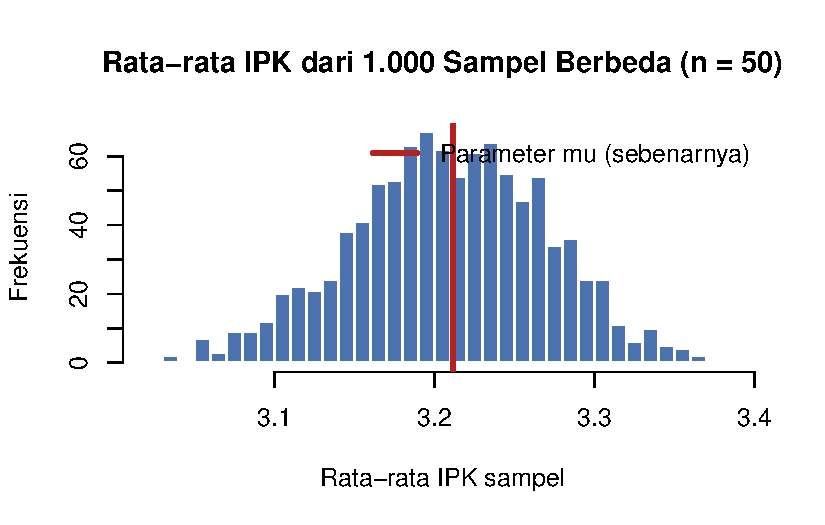
\includegraphics[keepaspectratio]{chapters/P01_files/figure-pdf/unnamed-chunk-16-1.pdf}}

\begin{Shaded}
\begin{Highlighting}[]
\FunctionTok{range}\NormalTok{(rata\_sampel\_50)}
\end{Highlighting}
\end{Shaded}

\begin{verbatim}
[1] 3.0284 3.3844
\end{verbatim}

Setiap sampel menghasilkan ̄𝑥 yang berbeda, tetapi nilai-nilainya
\textbf{berkumpul di sekitar 𝜇}. Inilah alasan statistika inferensial
selalu menyertakan ukuran ketidakpastian. \textbf{Pengaruh ukuran
sampel}. Apa yang terjadi jika sampel diperbesar?

\begin{Shaded}
\begin{Highlighting}[]
\FunctionTok{set.seed}\NormalTok{(}\DecValTok{3}\NormalTok{)}
\NormalTok{rata\_sampel\_10 }\OtherTok{\textless{}{-}} \FunctionTok{replicate}\NormalTok{(}\DecValTok{1000}\NormalTok{, }\FunctionTok{mean}\NormalTok{(}\FunctionTok{sample}\NormalTok{(populasi}\SpecialCharTok{$}\NormalTok{ipk, }\DecValTok{10}\NormalTok{)))}
\NormalTok{rata\_sampel\_200 }\OtherTok{\textless{}{-}} \FunctionTok{replicate}\NormalTok{(}\DecValTok{1000}\NormalTok{, }\FunctionTok{mean}\NormalTok{(}\FunctionTok{sample}\NormalTok{(populasi}\SpecialCharTok{$}\NormalTok{ipk, }\DecValTok{200}\NormalTok{)))}
\FunctionTok{par}\NormalTok{(}\AttributeTok{mfrow =} \FunctionTok{c}\NormalTok{(}\DecValTok{1}\NormalTok{, }\DecValTok{3}\NormalTok{))}
\ControlFlowTok{for}\NormalTok{ (hasil }\ControlFlowTok{in} \FunctionTok{list}\NormalTok{(}\FunctionTok{list}\NormalTok{(rata\_sampel\_10, }\StringTok{"n = 10"}\NormalTok{), }\FunctionTok{list}\NormalTok{(rata\_sampel\_50, }\StringTok{"n = 50"}\NormalTok{),}
\FunctionTok{list}\NormalTok{(rata\_sampel\_200, }\StringTok{"n = 200"}\NormalTok{))) \{}
\FunctionTok{hist}\NormalTok{(hasil[[}\DecValTok{1}\NormalTok{]], }\AttributeTok{breaks =} \DecValTok{25}\NormalTok{, }\AttributeTok{xlim =} \FunctionTok{c}\NormalTok{(}\FloatTok{2.9}\NormalTok{, }\FloatTok{3.5}\NormalTok{), }\AttributeTok{col =} \StringTok{"\#9ecae1"}\NormalTok{, }\AttributeTok{border =} \StringTok{"white"}\NormalTok{,}
\AttributeTok{main =}\NormalTok{ hasil[[}\DecValTok{2}\NormalTok{]], }\AttributeTok{xlab =} \StringTok{"Rata{-}rata IPK sampel"}\NormalTok{, }\AttributeTok{ylab =} \StringTok{"Frekuensi"}\NormalTok{)}
\FunctionTok{abline}\NormalTok{(}\AttributeTok{v =}\NormalTok{ mu, }\AttributeTok{col =} \StringTok{"firebrick"}\NormalTok{, }\AttributeTok{lwd =} \DecValTok{2}\NormalTok{)}
\NormalTok{\}}
\end{Highlighting}
\end{Shaded}

\pandocbounded{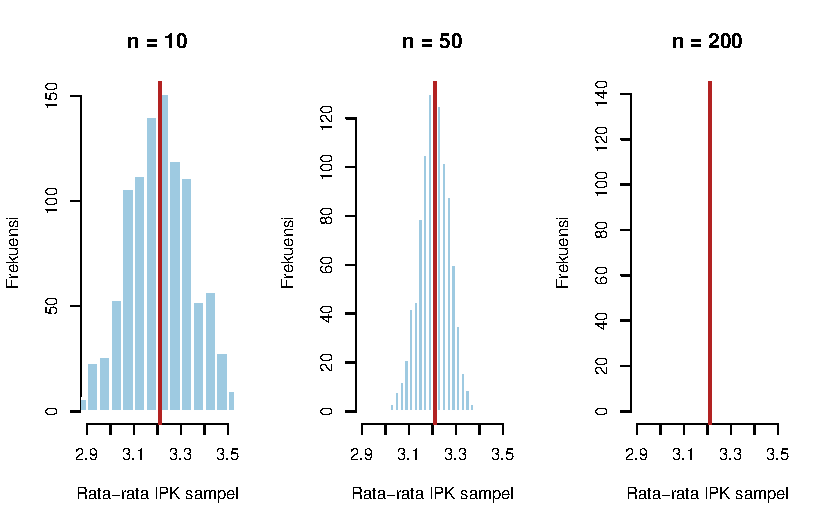
\includegraphics[keepaspectratio]{chapters/P01_files/figure-pdf/unnamed-chunk-18-1.pdf}}

\begin{Shaded}
\begin{Highlighting}[]
\FunctionTok{par}\NormalTok{(}\AttributeTok{mfrow =} \FunctionTok{c}\NormalTok{(}\DecValTok{1}\NormalTok{, }\DecValTok{1}\NormalTok{))}
\FunctionTok{round}\NormalTok{(}\FunctionTok{c}\NormalTok{(}\AttributeTok{Sebaran\_n10 =} \FunctionTok{sd}\NormalTok{(rata\_sampel\_10), }\AttributeTok{Sebaran\_n50 =} \FunctionTok{sd}\NormalTok{(rata\_sampel\_50),}
\AttributeTok{Sebaran\_n200 =} \FunctionTok{sd}\NormalTok{(rata\_sampel\_200)), }\DecValTok{4}\NormalTok{)}
\end{Highlighting}
\end{Shaded}

\begin{verbatim}
 Sebaran_n10  Sebaran_n50 Sebaran_n200 
      0.1358       0.0615       0.0292 
\end{verbatim}

Semakin besar sampel, semakin \textbf{sempit} sebaran ̄𝑥 di sekitar 𝜇 --
statistik semakin dapat dipercaya. Ide ini akan dibahas secara formal
pada Pertemuan 9 (\emph{sampling distribution} dan \emph{Central Limit
Theorem}).

\subsection{Sekilas Inferensi}\label{sekilas-inferensi}

Sebagai pratinjau, statistika inferensial memungkinkan kita menyatakan:
``berdasarkan satu sampel ini, \textbf{𝜇 kemungkinan besar} berada di
antara \ldots{} dan \ldots''.

\begin{Shaded}
\begin{Highlighting}[]
\NormalTok{se }\OtherTok{\textless{}{-}} \FunctionTok{sd}\NormalTok{(sampel}\SpecialCharTok{$}\NormalTok{ipk) }\SpecialCharTok{/} \FunctionTok{sqrt}\NormalTok{(n)}
\NormalTok{selang }\OtherTok{\textless{}{-}} \FunctionTok{c}\NormalTok{(}\AttributeTok{Bawah =}\NormalTok{ x\_bar }\SpecialCharTok{{-}} \DecValTok{2} \SpecialCharTok{*}\NormalTok{ se, }\AttributeTok{Atas =}\NormalTok{ x\_bar }\SpecialCharTok{+} \DecValTok{2} \SpecialCharTok{*}\NormalTok{ se)}
\FunctionTok{round}\NormalTok{(selang, }\DecValTok{3}\NormalTok{)}
\end{Highlighting}
\end{Shaded}

\begin{verbatim}
Bawah  Atas 
3.102 3.380 
\end{verbatim}

\begin{Shaded}
\begin{Highlighting}[]
\CommentTok{\# Apakah selang memuat parameter?}
\NormalTok{mu }\SpecialCharTok{\textgreater{}=}\NormalTok{ selang[}\StringTok{"Bawah"}\NormalTok{] }\SpecialCharTok{\&}\NormalTok{ mu }\SpecialCharTok{\textless{}=}\NormalTok{ selang[}\StringTok{"Atas"}\NormalTok{]}
\end{Highlighting}
\end{Shaded}

\begin{verbatim}
Bawah 
 TRUE 
\end{verbatim}

Rumus di atas \textbf{belum perlu dihafal}; yang penting adalah idenya:
kesimpulan tentang populasi dinyatakan sebagai \textbf{rentang} beserta
tingkat kepercayaannya, bukan satu angka pasti.

\section{Variabel}\label{variabel}

\textbf{Variabel} adalah karakteristik yang \textbf{nilainya bervariasi}
antarunit observasi. Dalam data frame, setiap kolom adalah satu
variabel.

\subsection{Variabel Numerik vs
Kategorik}\label{variabel-numerik-vs-kategorik}

{\def\LTcaptype{none} % do not increment counter
\begin{longtable}[]{@{}
  >{\raggedright\arraybackslash}p{(\linewidth - 6\tabcolsep) * \real{0.2500}}
  >{\raggedright\arraybackslash}p{(\linewidth - 6\tabcolsep) * \real{0.2500}}
  >{\raggedright\arraybackslash}p{(\linewidth - 6\tabcolsep) * \real{0.2500}}
  >{\raggedright\arraybackslash}p{(\linewidth - 6\tabcolsep) * \real{0.2500}}@{}}
\toprule\noalign{}
\begin{minipage}[b]{\linewidth}\raggedright
Jenis
\end{minipage} & \begin{minipage}[b]{\linewidth}\raggedright
Ciri
\end{minipage} & \begin{minipage}[b]{\linewidth}\raggedright
Contoh
\end{minipage} & \begin{minipage}[b]{\linewidth}\raggedright
Tipe di R
\end{minipage} \\
\midrule\noalign{}
\endhead
\bottomrule\noalign{}
\endlastfoot
\textbf{Numerik}(kuantitatif) & Nilainya angka yang \textbf{bermakna
untuk dihitung} (dijumlah, dirata-rata) & IPK, jam belajar, uang saku,
tinggi badan & \texttt{numeric}, \texttt{integer} \\
\textbf{Kategorik}(kualitatif) & Nilainya \textbf{label/kelompok} &
Fakultas, jenis kelamin, tempat tinggal & character, factor \\
\end{longtable}
}

\textbf{Jebakan penting}: tidak semua yang ditulis dengan angka adalah
variabel numerik. NIM, kode pos, nomor HP, atau kode fakultas ``1, 2,
3'' adalah \textbf{kategorik}, karena merata-ratakannya tidak bermakna.

\begin{Shaded}
\begin{Highlighting}[]
\FunctionTok{str}\NormalTok{(sampel)}
\end{Highlighting}
\end{Shaded}

\begin{verbatim}
'data.frame':   50 obs. of  7 variables:
 $ id         : int  1017 4775 2177 1533 4567 2347 270 4050 3379 4065 ...
 $ fakultas   : chr  "Ekonomi" "Ekonomi" "Sains" "Ekonomi" ...
 $ jenis_kel  : chr  "Perempuan" "Laki-laki" "Laki-laki" "Perempuan" ...
 $ tinggal    : chr  "Kos" "Kos" "Asrama" "Kos" ...
 $ jam_belajar: num  20.6 19.7 15.4 24.1 19.9 8.8 25.3 14.4 10.1 19.7 ...
 $ ipk        : num  3.53 3.39 3.77 3.66 3.25 2.59 4 2.55 2.46 3.53 ...
 $ uang_saku  : num  2.94 3.7 2.5 2.61 2.47 1.36 2.28 4.9 2.27 1.28 ...
\end{verbatim}

\begin{Shaded}
\begin{Highlighting}[]
\NormalTok{jenis\_variabel }\OtherTok{\textless{}{-}} \ControlFlowTok{function}\NormalTok{(x) }\ControlFlowTok{if}\NormalTok{ (}\FunctionTok{is.numeric}\NormalTok{(x)) }\StringTok{"Numerik"} \ControlFlowTok{else} \StringTok{"Kategorik"}
\FunctionTok{sapply}\NormalTok{(sampel, jenis\_variabel)}
\end{Highlighting}
\end{Shaded}

\begin{verbatim}
         id    fakultas   jenis_kel     tinggal jam_belajar         ipk 
  "Numerik" "Kategorik" "Kategorik" "Kategorik"   "Numerik"   "Numerik" 
  uang_saku 
  "Numerik" 
\end{verbatim}

Menurut R, kolom id bertipe numerik -- padahal secara makna id hanyalah
\textbf{label} unit observasi. R hanya melihat \textbf{tipe
penyimpanan}, sedangkan menentukan jenis variabel adalah tugas
\textbf{analis} 13 berdasarkan \textbf{makna}.

\begin{Shaded}
\begin{Highlighting}[]
\FunctionTok{mean}\NormalTok{(sampel}\SpecialCharTok{$}\NormalTok{id) }\CommentTok{\# dapat dihitung, tetapi "rata{-}rata nomor ID" tidak bermakna apapun}
\end{Highlighting}
\end{Shaded}

\begin{verbatim}
[1] 2248.94
\end{verbatim}

\begin{Shaded}
\begin{Highlighting}[]
\FunctionTok{table}\NormalTok{(sampel}\SpecialCharTok{$}\NormalTok{fakultas)}
\end{Highlighting}
\end{Shaded}

\begin{verbatim}

   Ekonomi      Hukum Kedokteran      Sains     Teknik 
        19          6          1         16          8 
\end{verbatim}

\begin{Shaded}
\begin{Highlighting}[]
\FunctionTok{summary}\NormalTok{(sampel}\SpecialCharTok{$}\NormalTok{jam\_belajar)}
\end{Highlighting}
\end{Shaded}

\begin{verbatim}
   Min. 1st Qu.  Median    Mean 3rd Qu.    Max. 
   2.10   11.32   14.45   15.19   19.98   25.80 
\end{verbatim}

Pembagian numerik menjadi \textbf{diskrit/kontinu} dan kategorik menjadi
\textbf{nominal/ordinal} akan dibahas lebih rinci pada Pertemuan 2.

\subsection{Variabel Independen vs
Dependen}\label{variabel-independen-vs-dependen}

Ketika sebuah studi menyelidiki \textbf{hubungan} antarvariabel, peran
variabel dibedakan:

{\def\LTcaptype{none} % do not increment counter
\begin{longtable}[]{@{}
  >{\raggedright\arraybackslash}p{(\linewidth - 6\tabcolsep) * \real{0.2500}}
  >{\raggedright\arraybackslash}p{(\linewidth - 6\tabcolsep) * \real{0.2500}}
  >{\raggedright\arraybackslash}p{(\linewidth - 6\tabcolsep) * \real{0.2500}}
  >{\raggedright\arraybackslash}p{(\linewidth - 6\tabcolsep) * \real{0.2500}}@{}}
\toprule\noalign{}
\begin{minipage}[b]{\linewidth}\raggedright
Peran
\end{minipage} & \begin{minipage}[b]{\linewidth}\raggedright
Nama lain
\end{minipage} & \begin{minipage}[b]{\linewidth}\raggedright
Makna
\end{minipage} & \begin{minipage}[b]{\linewidth}\raggedright
Contoh
\end{minipage} \\
\midrule\noalign{}
\endhead
\bottomrule\noalign{}
\endlastfoot
\textbf{Independen} & Variabel bebas, prediktor, \emph{feature}, \(X\) &
Variabel yang \textbf{diduga memengaruhi} & Jam belajar per minggu \\
\textbf{Dependen} & Variabel terikat, respons, \emph{target}, \(Y\) &
Variabel yang \textbf{diduga dipengaruhi} & IPK \\
\end{longtable}
}

\begin{Shaded}
\begin{Highlighting}[]
\FunctionTok{plot}\NormalTok{(sampel}\SpecialCharTok{$}\NormalTok{jam\_belajar, sampel}\SpecialCharTok{$}\NormalTok{ipk, }\AttributeTok{pch =} \DecValTok{16}\NormalTok{, }\AttributeTok{col =} \StringTok{"steelblue"}\NormalTok{,}
\AttributeTok{xlab =} \StringTok{"Jam belajar per minggu (variabel independen, X)"}\NormalTok{,}
\AttributeTok{ylab =} \StringTok{"IPK (variabel dependen, Y)"}\NormalTok{,}
\AttributeTok{main =} \StringTok{"Hubungan Jam Belajar dan IPK (n = 50)"}\NormalTok{)}
\FunctionTok{abline}\NormalTok{(}\FunctionTok{lm}\NormalTok{(ipk }\SpecialCharTok{\textasciitilde{}}\NormalTok{ jam\_belajar, }\AttributeTok{data =}\NormalTok{ sampel), }\AttributeTok{col =} \StringTok{"firebrick"}\NormalTok{, }\AttributeTok{lwd =} \DecValTok{2}\NormalTok{)}
\end{Highlighting}
\end{Shaded}

\pandocbounded{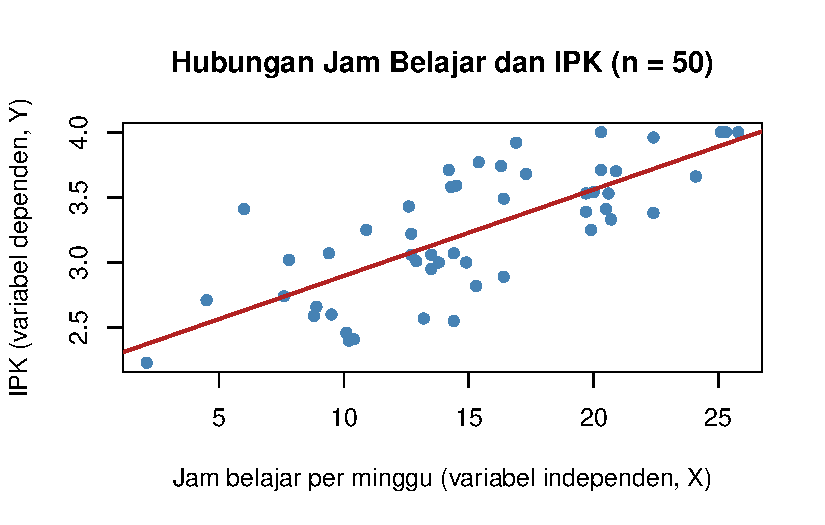
\includegraphics[keepaspectratio]{chapters/P01_files/figure-pdf/unnamed-chunk-27-1.pdf}}

Secara umum, mahasiswa yang belajar lebih lama cenderung memiliki IPK
lebih tinggi. Konvensi grafiknya: variabel independen di
\textbf{sumbu-x}, dependen di \textbf{sumbu-y}. Hubungan ini akan diukur
secara formal pada Pertemuan 15 (korelasi dan regresi).

\textbf{Peran variabel ditentukan oleh pertanyaan penelitian, bukan oleh
variabelnya}. ``IPK'' adalah variabel dependen jika pertanyaannya
``apakah jam belajar memengaruhi IPK?'', tetapi menjadi variabel
independen jika pertanyaannya ``apakah IPK memengaruhi gaji pertama
lulusan?''. \textbf{Hubungan belum tentu sebab-akibat}. Data survei
(observasional) hanya menunjukkan bahwa dua variabel bergerak bersama.
Untuk menyimpulkan sebab-akibat, dibutuhkan desain eksperimen (Pertemuan
3).

\section{Kerangka Membaca Sebuah
Studi}\label{kerangka-membaca-sebuah-studi}

Setiap kali menjumpai klaim berbasis data, biasakan menjawab enam
pertanyaan berikut:

{\def\LTcaptype{none} % do not increment counter
\begin{longtable}[]{@{}
  >{\raggedright\arraybackslash}p{(\linewidth - 4\tabcolsep) * \real{0.3333}}
  >{\raggedright\arraybackslash}p{(\linewidth - 4\tabcolsep) * \real{0.3333}}
  >{\raggedright\arraybackslash}p{(\linewidth - 4\tabcolsep) * \real{0.3333}}@{}}
\toprule\noalign{}
\begin{minipage}[b]{\linewidth}\raggedright
No
\end{minipage} & \begin{minipage}[b]{\linewidth}\raggedright
Pertanyaan
\end{minipage} & \begin{minipage}[b]{\linewidth}\raggedright
Mengidentifikasi
\end{minipage} \\
\midrule\noalign{}
\endhead
\bottomrule\noalign{}
\endlastfoot
1 & Kesimpulannya ditujukan kepada siapa? & \textbf{Populasi} \\
2 & Siapa yang benar-benar diamati, dan berapa banyak? & \textbf{Sampel}
dan \(n\) \\
3 & Satu baris data mewakili apa? & \textbf{Unit observasi} \\
4 & Karakteristik apa yang diukur, dan apa jenisnya? & \textbf{Variabel}
(numerik/kategorik) \\
5 & Angka yang dilaporkan dihitung dari sampel atau populasi? &
\textbf{Statistik} atau \textbf{parameter} \\
6 & Apakah klaimnya hanya menggambarkan data, atau menggeneralisasi? &
\textbf{Deskriptif} atau \textbf{inferensial} \\
\end{longtable}
}

\section{Studi Kasus Komprehensif: Survei Pemakaian
QRIS}\label{studi-kasus-komprehensif-survei-pemakaian-qris}

\textbf{Konteks}: Sebuah lembaga riset melaporkan: \emph{``Survei
terhadap 400 pelaku UMKM kuliner di Kota Bandung menunjukkan 72\% sudah
menerima pembayaran QRIS, dengan rata-rata 38 transaksi QRIS per minggu.
Pelaku usaha yang lebih lama memakai QRIS cenderung memiliki omzet lebih
tinggi.Dengan demikian, sekitar tujuh dari sepuluh UMKM kuliner di
Bandung telah mengadopsi QRIS.''} Kita simulasikan data survei tersebut
agar dapat dianalisis.

\begin{Shaded}
\begin{Highlighting}[]
\FunctionTok{set.seed}\NormalTok{(}\DecValTok{2024}\NormalTok{)}
\NormalTok{n\_umkm }\OtherTok{\textless{}{-}} \DecValTok{400}
\NormalTok{umkm }\OtherTok{\textless{}{-}} \FunctionTok{data.frame}\NormalTok{(}
\AttributeTok{id\_umkm =} \FunctionTok{sprintf}\NormalTok{(}\StringTok{"UMKM{-}\%03d"}\NormalTok{, }\DecValTok{1}\SpecialCharTok{:}\NormalTok{n\_umkm),}
\AttributeTok{jenis\_usaha =} \FunctionTok{sample}\NormalTok{(}\FunctionTok{c}\NormalTok{(}\StringTok{"Warung makan"}\NormalTok{, }\StringTok{"Kedai kopi"}\NormalTok{, }\StringTok{"Kue \& roti"}\NormalTok{, }\StringTok{"Streetfood"}\NormalTok{),}
\NormalTok{n\_umkm, }\AttributeTok{replace =} \ConstantTok{TRUE}\NormalTok{),}
\AttributeTok{terima\_qris =} \FunctionTok{sample}\NormalTok{(}\FunctionTok{c}\NormalTok{(}\StringTok{"Ya"}\NormalTok{, }\StringTok{"Tidak"}\NormalTok{), n\_umkm, }\AttributeTok{replace =} \ConstantTok{TRUE}\NormalTok{, }\AttributeTok{prob =} \FunctionTok{c}\NormalTok{(}\FloatTok{0.72}\NormalTok{, }\FloatTok{0.28}\NormalTok{))}
\NormalTok{)}
\NormalTok{umkm}\SpecialCharTok{$}\NormalTok{bulan\_qris }\OtherTok{\textless{}{-}} \FunctionTok{ifelse}\NormalTok{(umkm}\SpecialCharTok{$}\NormalTok{terima\_qris }\SpecialCharTok{==} \StringTok{"Ya"}\NormalTok{, }\FunctionTok{sample}\NormalTok{(}\DecValTok{1}\SpecialCharTok{:}\DecValTok{48}\NormalTok{, n\_umkm, }\AttributeTok{replace =} \ConstantTok{TRUE}\NormalTok{), }\DecValTok{0}\NormalTok{)}
\NormalTok{umkm}\SpecialCharTok{$}\NormalTok{trx\_qris }\OtherTok{\textless{}{-}} \FunctionTok{ifelse}\NormalTok{(umkm}\SpecialCharTok{$}\NormalTok{terima\_qris }\SpecialCharTok{==} \StringTok{"Ya"}\NormalTok{,}
\FunctionTok{rpois}\NormalTok{(n\_umkm, }\AttributeTok{lambda =} \DecValTok{20} \SpecialCharTok{+} \FloatTok{0.75} \SpecialCharTok{*}\NormalTok{ umkm}\SpecialCharTok{$}\NormalTok{bulan\_qris), }\DecValTok{0}\NormalTok{)}
\NormalTok{umkm}\SpecialCharTok{$}\NormalTok{omzet\_juta }\OtherTok{\textless{}{-}} \FunctionTok{round}\NormalTok{(}\FunctionTok{rlnorm}\NormalTok{(n\_umkm, }\FunctionTok{log}\NormalTok{(}\DecValTok{15} \SpecialCharTok{+} \FloatTok{0.25} \SpecialCharTok{*}\NormalTok{ umkm}\SpecialCharTok{$}\NormalTok{bulan\_qris), }\FloatTok{0.35}\NormalTok{), }\DecValTok{1}\NormalTok{)}
\FunctionTok{str}\NormalTok{(umkm)}
\end{Highlighting}
\end{Shaded}

\begin{verbatim}
'data.frame':   400 obs. of  6 variables:
 $ id_umkm    : chr  "UMKM-001" "UMKM-002" "UMKM-003" "UMKM-004" ...
 $ jenis_usaha: chr  "Kedai kopi" "Warung makan" "Warung makan" "Streetfood" ...
 $ terima_qris: chr  "Ya" "Tidak" "Ya" "Tidak" ...
 $ bulan_qris : num  47 0 39 0 8 24 21 38 0 0 ...
 $ trx_qris   : num  54 0 44 0 33 37 34 43 0 0 ...
 $ omzet_juta : num  22.1 15.8 25.6 13.8 14.3 23.9 25.5 24.4 15.5 9.7 ...
\end{verbatim}

\subsection{Langkah 1: Identifikasi Komponen
Studi}\label{langkah-1-identifikasi-komponen-studi}

{\def\LTcaptype{none} % do not increment counter
\begin{longtable}[]{@{}
  >{\raggedright\arraybackslash}p{(\linewidth - 2\tabcolsep) * \real{0.5000}}
  >{\raggedright\arraybackslash}p{(\linewidth - 2\tabcolsep) * \real{0.5000}}@{}}
\toprule\noalign{}
\begin{minipage}[b]{\linewidth}\raggedright
Komponen
\end{minipage} & \begin{minipage}[b]{\linewidth}\raggedright
Jawaban
\end{minipage} \\
\midrule\noalign{}
\endhead
\bottomrule\noalign{}
\endlastfoot
Populasi & Seluruh pelaku UMKM kuliner di Kota Bandung \\
Sampel & 400 pelaku UMKM kuliner yang disurvei \\
Unit observasi & Satu UMKM kuliner \\
Variabel kategorik & \texttt{jenis\_usaha}, \texttt{terima\_qris} (dan
\texttt{id\_umkm} sebagai label) \\
Variabel numerik & \texttt{bulan\_qris}, \texttt{trx\_qris},
\texttt{omzet\_juta} \\
Statistik & 72\% (proporsi penerima QRIS dalam sampel); 38 transaksi
(rata-rata sampel) \\
Parameter yang diduga & Proporsi dan rata-rata transaksi pada
\textbf{seluruh} UMKM kuliner Bandung \\
\end{longtable}
}

\subsection{Langkah 2: Menghitung Statistik dari
Sampel}\label{langkah-2-menghitung-statistik-dari-sampel}

\begin{Shaded}
\begin{Highlighting}[]
\NormalTok{p\_hat\_qris }\OtherTok{\textless{}{-}} \FunctionTok{mean}\NormalTok{(umkm}\SpecialCharTok{$}\NormalTok{terima\_qris }\SpecialCharTok{==} \StringTok{"Ya"}\NormalTok{)}
\NormalTok{rata\_trx }\OtherTok{\textless{}{-}} \FunctionTok{mean}\NormalTok{(umkm}\SpecialCharTok{$}\NormalTok{trx\_qris[umkm}\SpecialCharTok{$}\NormalTok{terima\_qris }\SpecialCharTok{==} \StringTok{"Ya"}\NormalTok{])}
\FunctionTok{c}\NormalTok{(}\AttributeTok{Proporsi\_QRIS =} \FunctionTok{round}\NormalTok{(p\_hat\_qris, }\DecValTok{3}\NormalTok{), }\AttributeTok{Rata\_trx\_per\_minggu =} \FunctionTok{round}\NormalTok{(rata\_trx, }\DecValTok{1}\NormalTok{))}
\end{Highlighting}
\end{Shaded}

\begin{verbatim}
      Proporsi_QRIS Rata_trx_per_minggu 
              0.715              36.100 
\end{verbatim}

\begin{Shaded}
\begin{Highlighting}[]
\FunctionTok{table}\NormalTok{(umkm}\SpecialCharTok{$}\NormalTok{jenis\_usaha, umkm}\SpecialCharTok{$}\NormalTok{terima\_qris)}
\end{Highlighting}
\end{Shaded}

\begin{verbatim}
              
               Tidak Ya
  Kedai kopi      21 70
  Kue & roti      23 73
  Streetfood      26 75
  Warung makan    44 68
\end{verbatim}

Karena datanya hasil simulasi, angkanya (71.5\% dan 36.1 transaksi)
sedikit berbeda dari laporan (72\% dan 38 transaksi) -- persis seperti
dua sampel berbeda yang menghasilkan statistik berbeda.

\subsection{Langkah 3: Variabel Independen dan
Dependen}\label{langkah-3-variabel-independen-dan-dependen}

\begin{Shaded}
\begin{Highlighting}[]
\NormalTok{pengguna }\OtherTok{\textless{}{-}} \FunctionTok{subset}\NormalTok{(umkm, terima\_qris }\SpecialCharTok{==} \StringTok{"Ya"}\NormalTok{)}
\FunctionTok{plot}\NormalTok{(pengguna}\SpecialCharTok{$}\NormalTok{bulan\_qris, pengguna}\SpecialCharTok{$}\NormalTok{omzet\_juta, }\AttributeTok{pch =} \DecValTok{16}\NormalTok{, }\AttributeTok{col =} \FunctionTok{rgb}\NormalTok{(}\FloatTok{0.3}\NormalTok{, }\FloatTok{0.45}\NormalTok{, }\FloatTok{0.7}\NormalTok{, }\FloatTok{0.6}\NormalTok{),}
\AttributeTok{xlab =} \StringTok{"Lama memakai QRIS (bulan) {-}{-} independen"}\NormalTok{,}
\AttributeTok{ylab =} \StringTok{"Omzet per bulan (juta Rp) {-}{-} dependen"}\NormalTok{,}
\AttributeTok{main =} \StringTok{"Lama Pemakaian QRIS vs Omzet UMKM"}\NormalTok{)}
\FunctionTok{abline}\NormalTok{(}\FunctionTok{lm}\NormalTok{(omzet\_juta }\SpecialCharTok{\textasciitilde{}}\NormalTok{ bulan\_qris, }\AttributeTok{data =}\NormalTok{ pengguna), }\AttributeTok{col =} \StringTok{"firebrick"}\NormalTok{, }\AttributeTok{lwd =} \DecValTok{2}\NormalTok{)}
\end{Highlighting}
\end{Shaded}

\pandocbounded{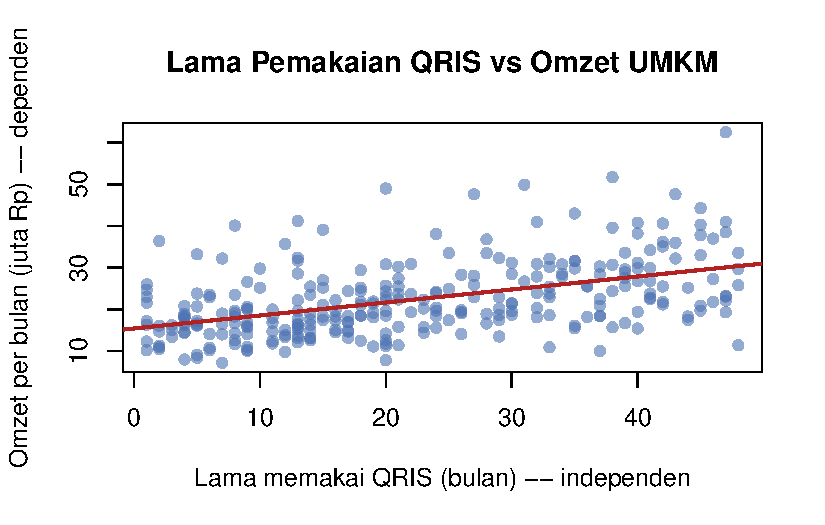
\includegraphics[keepaspectratio]{chapters/P01_files/figure-pdf/unnamed-chunk-31-1.pdf}}

\subsection{Pertanyaan Diskusi dan
Jawaban}\label{pertanyaan-diskusi-dan-jawaban}

\textbf{1. Bagian mana dari laporan itu yang deskriptif, dan mana yang
inferensial?} ``72\% sudah menerima QRIS'' dan ``rata-rata 38
transaksi'' adalah \textbf{deskriptif} (menggambarkan 400 UMKM dalam
sampel). Kalimat ``sekitar tujuh dari sepuluh UMKM kuliner \textbf{di
Bandung''} adalah \textbf{inferensial} karena menggeneralisasi ke
seluruh populasi. 2. Apakah generalisasi tersebut sah? Hanya jika sampel
400 UMKM \textbf{mewakili} populasi -- misalnya dipilih secara acak dari
daftar seluruh UMKM kuliner Bandung. Jika survei dilakukan secara online
melalui media sosial, UMKM yang sudah melek digital akan lebih banyak
terjaring, dan angka 72\% kemungkinan \textbf{terlalu tinggi}. Laporan
juga sebaiknya menyebut ketidakpastiannya (misalnya \emph{margin of
error}). \textbf{3. Bolehkah disimpulkan bahwa ``memakai QRIS
menyebabkan omzet naik''?} \textbf{Tidak.} Grafik menunjukkan
\textbf{kecenderungan bersama}, tetapi data ini observasional. Bisa jadi
UMKM yang omzetnya sudah besar lebih dahulu mengadopsi QRIS (arah
sebab-akibat terbalik), atau ada faktor lain (lokasi strategis) yang
memengaruhi keduanya. \textbf{4. Mengapa id\_umkm tidak dianalisis?}
id\_umkm hanya \textbf{pengenal} unit observasi. Ia bukan karakteristik
yang bervariasi secara bermakna, sehingga tidak dianalisis sebagai
variabel.

\section{Latihan Mandiri}\label{latihan-mandiri}

\subsection{Latihan Utama: Survei Kepuasan Aplikasi
Kampus}\label{latihan-utama-survei-kepuasan-aplikasi-kampus}

\textbf{Konteks}: Bagian TI sebuah universitas dengan 12.000 mahasiswa
ingin mengetahui kepuasan terhadap aplikasi akademik barunya. Mereka
menyebarkan kuesioner kepada 300 mahasiswa yang dipilih acak dari daftar
mahasiswa aktif. Laporan awal menyebut: skor kepuasan rata-rata sekitar
3,5 (skala 1--5), sekitar 60\% mahasiswa mengakses aplikasi setiap hari,
dan mahasiswa yang lebih sering mengalami error cenderung memberi skor
kepuasan lebih rendah.

\begin{Shaded}
\begin{Highlighting}[]
\FunctionTok{set.seed}\NormalTok{(}\DecValTok{77}\NormalTok{)}
\NormalTok{survei\_app }\OtherTok{\textless{}{-}} \FunctionTok{data.frame}\NormalTok{(}
\AttributeTok{nim =} \FunctionTok{sprintf}\NormalTok{(}\StringTok{"2024\%04d"}\NormalTok{, }\FunctionTok{sample}\NormalTok{(}\DecValTok{1}\SpecialCharTok{:}\DecValTok{9999}\NormalTok{, }\DecValTok{300}\NormalTok{)),}
\AttributeTok{angkatan =} \FunctionTok{sample}\NormalTok{(}\DecValTok{2021}\SpecialCharTok{:}\DecValTok{2024}\NormalTok{, }\DecValTok{300}\NormalTok{, }\AttributeTok{replace =} \ConstantTok{TRUE}\NormalTok{),}
\AttributeTok{akses\_harian =} \FunctionTok{sample}\NormalTok{(}\FunctionTok{c}\NormalTok{(}\StringTok{"Ya"}\NormalTok{, }\StringTok{"Tidak"}\NormalTok{), }\DecValTok{300}\NormalTok{, }\AttributeTok{replace =} \ConstantTok{TRUE}\NormalTok{, }\AttributeTok{prob =} \FunctionTok{c}\NormalTok{(}\FloatTok{0.64}\NormalTok{, }\FloatTok{0.36}\NormalTok{)),}
\AttributeTok{jumlah\_error =} \FunctionTok{rpois}\NormalTok{(}\DecValTok{300}\NormalTok{, }\AttributeTok{lambda =} \DecValTok{3}\NormalTok{)}
\NormalTok{)}
\NormalTok{survei\_app}\SpecialCharTok{$}\NormalTok{kepuasan }\OtherTok{\textless{}{-}} \FunctionTok{pmin}\NormalTok{(}\DecValTok{5}\NormalTok{, }\FunctionTok{pmax}\NormalTok{(}\DecValTok{1}\NormalTok{, }\FunctionTok{round}\NormalTok{(}\FloatTok{4.4} \SpecialCharTok{{-}} \FloatTok{0.25} \SpecialCharTok{*}\NormalTok{ survei\_app}\SpecialCharTok{$}\NormalTok{jumlah\_error }\SpecialCharTok{+}
\FunctionTok{rnorm}\NormalTok{(}\DecValTok{300}\NormalTok{, }\DecValTok{0}\NormalTok{, }\FloatTok{0.6}\NormalTok{))))}
\FunctionTok{head}\NormalTok{(survei\_app)}
\end{Highlighting}
\end{Shaded}

\begin{verbatim}
       nim angkatan akses_harian jumlah_error kepuasan
1 20242706     2021           Ya            6        4
2 20247365     2024        Tidak            1        3
3 20246648     2022           Ya            1        5
4 20246326     2022           Ya            3        3
5 20244416     2024           Ya            4        3
6 20248022     2024        Tidak            1        4
\end{verbatim}

\subsubsection{Tugas 1: Identifikasi komponen
studi}\label{tugas-1-identifikasi-komponen-studi}

Tentukan populasi, sampel, 𝑛, unit observasi, serta satu contoh
parameter dan statistik. \textbf{Jawaban}: Populasi = seluruh 12.000
mahasiswa aktif; sampel = 300 mahasiswa yang mengisi kuesioner (𝑛 =
300); unit observasi = satu mahasiswa. Parameter = proporsi
\textbf{seluruh} mahasiswa yang mengakses aplikasi setiap hari (tidak
diketahui); statistik = proporsi mahasiswa dalam sampel yang mengakses
aplikasi setiap hari (dihitung pada Tugas 3, sekitar 62.3\%).

\subsubsection{Tugas 2: Klasifikasikan setiap
variabel}\label{tugas-2-klasifikasikan-setiap-variabel}

\begin{Shaded}
\begin{Highlighting}[]
\FunctionTok{sapply}\NormalTok{(survei\_app, class)}
\end{Highlighting}
\end{Shaded}

\begin{verbatim}
         nim     angkatan akses_harian jumlah_error     kepuasan 
 "character"    "integer"  "character"    "integer"    "numeric" 
\end{verbatim}

\textbf{Jawaban}: akses\_harian kategorik; jumlah\_error numerik;
kepuasan pada skala 1--5 adalah \textbf{kategorik berurutan} (ordinal)
meskipun ditulis sebagai angka -- dibahas lebih lanjut di Pertemuan 2.
nim adalah label (kategorik, disimpan sebagai teks). angkatan tersimpan
sebagai numerik, tetapi dalam survei ini berfungsi sebagai
\textbf{kelompok} (kategorik).

\subsubsection{Tugas 3: Hitung statistik
sampel}\label{tugas-3-hitung-statistik-sampel}

\begin{Shaded}
\begin{Highlighting}[]
\FunctionTok{c}\NormalTok{(}\AttributeTok{Proporsi\_akses\_harian =} \FunctionTok{mean}\NormalTok{(survei\_app}\SpecialCharTok{$}\NormalTok{akses\_harian }\SpecialCharTok{==} \StringTok{"Ya"}\NormalTok{),}
\AttributeTok{Rata\_kepuasan =} \FunctionTok{mean}\NormalTok{(survei\_app}\SpecialCharTok{$}\NormalTok{kepuasan),}
\AttributeTok{Rata\_error =} \FunctionTok{mean}\NormalTok{(survei\_app}\SpecialCharTok{$}\NormalTok{jumlah\_error))}
\end{Highlighting}
\end{Shaded}

\begin{verbatim}
Proporsi_akses_harian         Rata_kepuasan            Rata_error 
            0.6233333             3.5266667             3.1033333 
\end{verbatim}

\subsubsection{Tugas 4: Tentukan variabel independen dan
dependen}\label{tugas-4-tentukan-variabel-independen-dan-dependen}

\begin{Shaded}
\begin{Highlighting}[]
\FunctionTok{boxplot}\NormalTok{(kepuasan }\SpecialCharTok{\textasciitilde{}}\NormalTok{ jumlah\_error, }\AttributeTok{data =}\NormalTok{ survei\_app, }\AttributeTok{col =} \StringTok{"\#c6dbef"}\NormalTok{,}
\AttributeTok{xlab =} \StringTok{"Jumlah error yang dialami (independen)"}\NormalTok{,}
\AttributeTok{ylab =} \StringTok{"Skor kepuasan (dependen)"}\NormalTok{, }\AttributeTok{main =} \StringTok{"Error vs Kepuasan"}\NormalTok{)}
\end{Highlighting}
\end{Shaded}

\pandocbounded{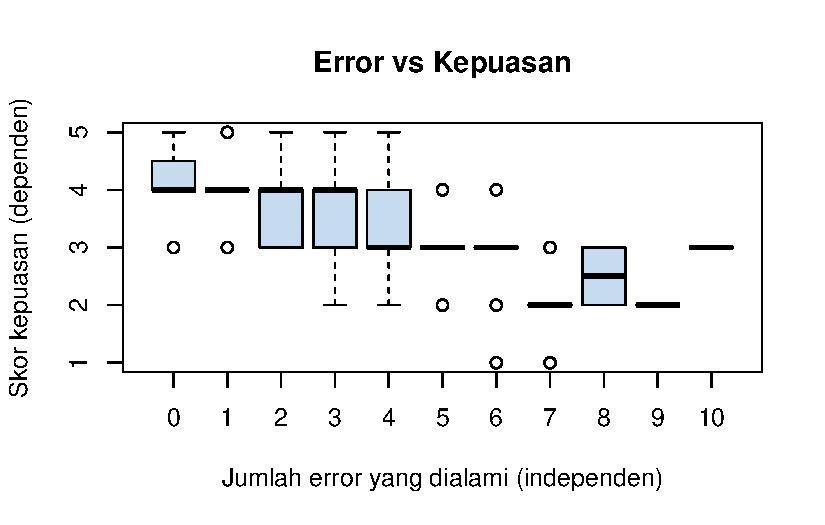
\includegraphics[keepaspectratio]{chapters/P01_files/figure-pdf/unnamed-chunk-35-1.pdf}}

\textbf{Jawaban}: Pertanyaannya adalah ``apakah error memengaruhi
kepuasan?'', sehingga jumlah\_error = \textbf{independen} dan kepuasan =
\textbf{dependen}. Grafik menunjukkan skor kepuasan cenderung turun
seiring bertambahnya error.

\subsubsection{Tugas 5: Deskriptif atau
inferensial?}\label{tugas-5-deskriptif-atau-inferensial}

Klasifikasikan dua kalimat berikut: (a) ``Rata-rata kepuasan 300
responden adalah 3,5.'' (b) ``Mayoritas mahasiswa universitas ini puas
terhadap aplikasi akademik.'' \textbf{Jawaban}: (a) \textbf{deskriptif}
-- hanya melaporkan sampel. (b) \textbf{inferensial} -- menggeneralisasi
ke seluruh mahasiswa; sah karena sampel diambil \textbf{acak} dari
daftar mahasiswa aktif, tetapi sebaiknya disertai ukuran ketidakpastian.

\subsubsection{Tugas 6 (Tantangan): Variabilitas
Sampling}\label{tugas-6-tantangan-variabilitas-sampling}

Anggap survei\_app sebagai populasi mini. Ambil 500 sampel acak
berukuran 30, hitung proporsi akses\_harian == ``Ya'' pada tiap sampel,
dan gambarkan histogramnya.

\begin{Shaded}
\begin{Highlighting}[]
\FunctionTok{set.seed}\NormalTok{(}\DecValTok{8}\NormalTok{)}
\NormalTok{prop\_30 }\OtherTok{\textless{}{-}} \FunctionTok{replicate}\NormalTok{(}\DecValTok{500}\NormalTok{, }\FunctionTok{mean}\NormalTok{(}\FunctionTok{sample}\NormalTok{(survei\_app}\SpecialCharTok{$}\NormalTok{akses\_harian, }\DecValTok{30}\NormalTok{) }\SpecialCharTok{==} \StringTok{"Ya"}\NormalTok{))}
\FunctionTok{hist}\NormalTok{(prop\_30, }\AttributeTok{breaks =} \DecValTok{15}\NormalTok{, }\AttributeTok{col =} \StringTok{"\#fdae6b"}\NormalTok{, }\AttributeTok{border =} \StringTok{"white"}\NormalTok{,}
\AttributeTok{main =} \StringTok{"Proporsi Akses Harian dari 500 Sampel (n = 30)"}\NormalTok{,}
\AttributeTok{xlab =} \StringTok{"Proporsi sampel"}\NormalTok{, }\AttributeTok{ylab =} \StringTok{"Frekuensi"}\NormalTok{)}
\FunctionTok{abline}\NormalTok{(}\AttributeTok{v =} \FunctionTok{mean}\NormalTok{(survei\_app}\SpecialCharTok{$}\NormalTok{akses\_harian }\SpecialCharTok{==} \StringTok{"Ya"}\NormalTok{), }\AttributeTok{col =} \StringTok{"firebrick"}\NormalTok{, }\AttributeTok{lwd =} \DecValTok{2}\NormalTok{)}
\end{Highlighting}
\end{Shaded}

\pandocbounded{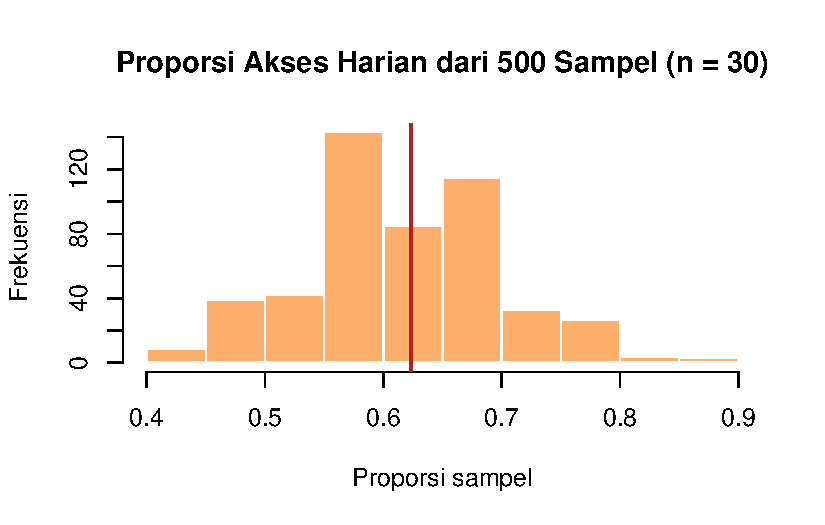
\includegraphics[keepaspectratio]{chapters/P01_files/figure-pdf/unnamed-chunk-36-1.pdf}}

\begin{Shaded}
\begin{Highlighting}[]
\FunctionTok{range}\NormalTok{(prop\_30)}
\end{Highlighting}
\end{Shaded}

\begin{verbatim}
[1] 0.4000000 0.8666667
\end{verbatim}

\textbf{Jawaban}: Proporsi sampel berkisar cukup lebar di sekitar
proporsi ``populasi'' (garis merah). Dengan 𝑛 = 30 saja, satu sampel
bisa menghasilkan angka yang cukup jauh dari nilai sebenarnya -- itulah
mengapa ukuran sampel dan ketidakpastian penting.

\subsection{Latihan Tambahan
(Self-Check)}\label{latihan-tambahan-self-check}

Kerjakan soal-soal berikut secara mandiri sebelum melihat kunci jawaban
pada komentar kode. \textbf{Soal A}. Sebuah pabrik baterai memproduksi
50.000 baterai per hari. Petugas QC menguji umur 100 baterai dan
mendapatkan rata-rata 18,2 jam. Tentukan populasi, sampel, parameter,
statistik, dan jelaskan mengapa sensus tidak mungkin dilakukan.

\begin{Shaded}
\begin{Highlighting}[]
\CommentTok{\# Kunci jawaban:}
\CommentTok{\# Populasi : seluruh 50.000 baterai produksi hari itu}
\CommentTok{\# Sampel : 100 baterai yang diuji (n = 100)}
\CommentTok{\# Parameter : rata{-}rata umur SELURUH 50.000 baterai (mu, tidak diketahui)}
\CommentTok{\# Statistik : x{-}bar = 18,2 jam}
\CommentTok{\# Sensus tidak mungkin karena pengujian umur bersifat MERUSAK (baterai habis dipakai).}
\end{Highlighting}
\end{Shaded}

\textbf{Soal B}. Klasifikasikan variabel berikut sebagai numerik atau
kategorik: (1) nomor kursi pesawat, (2) berat bagasi, (3) kelas
penerbangan (Ekonomi/Bisnis), (4) jumlah transit, (5) kode bandara (CGK,
DPS), (6) lama penerbangan.

\begin{Shaded}
\begin{Highlighting}[]
\CommentTok{\# Kunci jawaban:}
\CommentTok{\# (1) Kategorik (label, meskipun memuat angka) (2) Numerik}
\CommentTok{\# (3) Kategorik (4) Numerik}
\CommentTok{\# (5) Kategorik (6) Numerik}
\end{Highlighting}
\end{Shaded}

\textbf{Soal C}. Buat data frame berisi 6 teman sekelas dengan variabel:
nama, asal\_daerah, tinggi\_cm, jumlah\_saudara. Tampilkan strukturnya
dengan str() dan hitung rata-rata tinggi badan. Apakah angka ini
parameter atau statistik jika tujuannya menggambarkan seluruh angkatan?

\begin{Shaded}
\begin{Highlighting}[]
\NormalTok{teman }\OtherTok{\textless{}{-}} \FunctionTok{data.frame}\NormalTok{(}
\AttributeTok{nama =} \FunctionTok{c}\NormalTok{(}\StringTok{"A"}\NormalTok{, }\StringTok{"B"}\NormalTok{, }\StringTok{"C"}\NormalTok{, }\StringTok{"D"}\NormalTok{, }\StringTok{"E"}\NormalTok{, }\StringTok{"F"}\NormalTok{),}
\AttributeTok{asal\_daerah =} \FunctionTok{c}\NormalTok{(}\StringTok{"Bekasi"}\NormalTok{, }\StringTok{"Medan"}\NormalTok{, }\StringTok{"Bogor"}\NormalTok{, }\StringTok{"Makassar"}\NormalTok{, }\StringTok{"Bekasi"}\NormalTok{, }\StringTok{"Solo"}\NormalTok{),}
\AttributeTok{tinggi\_cm =} \FunctionTok{c}\NormalTok{(}\DecValTok{158}\NormalTok{, }\DecValTok{170}\NormalTok{, }\DecValTok{165}\NormalTok{, }\DecValTok{175}\NormalTok{, }\DecValTok{162}\NormalTok{, }\DecValTok{168}\NormalTok{),}
\AttributeTok{jumlah\_saudara =} \FunctionTok{c}\NormalTok{(}\DecValTok{2}\NormalTok{, }\DecValTok{1}\NormalTok{, }\DecValTok{3}\NormalTok{, }\DecValTok{0}\NormalTok{, }\DecValTok{2}\NormalTok{, }\DecValTok{4}\NormalTok{)}
\NormalTok{)}
\FunctionTok{str}\NormalTok{(teman)}
\end{Highlighting}
\end{Shaded}

\begin{verbatim}
'data.frame':   6 obs. of  4 variables:
 $ nama          : chr  "A" "B" "C" "D" ...
 $ asal_daerah   : chr  "Bekasi" "Medan" "Bogor" "Makassar" ...
 $ tinggi_cm     : num  158 170 165 175 162 168
 $ jumlah_saudara: num  2 1 3 0 2 4
\end{verbatim}

\begin{Shaded}
\begin{Highlighting}[]
\FunctionTok{mean}\NormalTok{(teman}\SpecialCharTok{$}\NormalTok{tinggi\_cm)}
\end{Highlighting}
\end{Shaded}

\begin{verbatim}
[1] 166.3333
\end{verbatim}

\begin{Shaded}
\begin{Highlighting}[]
\CommentTok{\# Kunci: rata{-}rata 6 orang adalah STATISTIK, karena 6 teman hanyalah sampel dari angkatan.}
\CommentTok{\# Namun jika tujuannya hanya menggambarkan 6 orang itu saja, keenamnya adalah populasi}
\CommentTok{\# dan angka tersebut menjadi parameter. Populasi ditentukan oleh TUJUAN kesimpulan.}
\end{Highlighting}
\end{Shaded}

\textbf{Soal D}. Seorang peneliti ingin mengetahui apakah durasi tidur
memengaruhi konsentrasi belajar. Tentukan variabel independen dan
dependen. Jika ia hanya mengamati (tanpa mengatur durasi tidur
responden), bolehkah ia menyimpulkan sebab-akibat?

\begin{Shaded}
\begin{Highlighting}[]
\CommentTok{\# Kunci jawaban:}
\CommentTok{\# Independen: durasi tidur; Dependen: skor konsentrasi belajar.}
\CommentTok{\# Karena hanya mengamati (studi observasional), ia hanya boleh menyimpulkan ADANYA HUBUNGAN,}
\CommentTok{\# bukan sebab{-}akibat. Faktor lain (stres, konsumsi kafein) bisa memengaruhi keduanya.}
\end{Highlighting}
\end{Shaded}

\section{Kesalahan Umum pada Konsep
Dasar}\label{kesalahan-umum-pada-konsep-dasar}

\begin{enumerate}
\def\labelenumi{\arabic{enumi}.}
\tightlist
\item
  Menyamakan ``statistika'' dan ``statistik'' -- yang pertama ilmunya,
  yang kedua nilai ringkasan dari sampel.
\item
  Menganggap statistik sampel sama persis dengan parameter -- selalu ada
  kesalahan sampling.
\item
  Menggeneralisasi dari sampel yang tidak mewakili -- misalnya survei
  online untuk menggambarkan seluruh penduduk.
\item
  Menyebut parameter sebagai sesuatu yang ``dihitung dari sampel'' --
  parameter adalah milik populasi dan biasanya tidak diketahui.
\item
  Menganggap variabel berkode angka sebagai numerik -- NIM, kode pos,
  dan kode kategori adalah kategorik.
\item
  Mengandalkan class() di R untuk menentukan jenis variabel -- R hanya
  tahu tipe penyimpanan, bukan makna.
\item
  Salah menentukan unit observasi -- sehingga kesimpulan tingkat
  kelompok dianggap berlaku untuk individu (ecological fallacy).
\item
  Menganggap peran independen/dependen melekat pada variabel -- perannya
  ditentukan pertanyaan penelitian.
\item
  Menyimpulkan sebab-akibat dari data observasional -- hubungan bukan
  berarti penyebab.
\item
  Melaporkan kesimpulan inferensial tanpa ketidakpastian -- generalisasi
  harus disertai margin of error atau selang kepercayaan.
\end{enumerate}

\section{Cheat Sheet: Fungsi R yang
Digunakan}\label{cheat-sheet-fungsi-r-yang-digunakan}

{\def\LTcaptype{none} % do not increment counter
\begin{longtable}[]{@{}
  >{\raggedright\arraybackslash}p{(\linewidth - 2\tabcolsep) * \real{0.5000}}
  >{\raggedright\arraybackslash}p{(\linewidth - 2\tabcolsep) * \real{0.5000}}@{}}
\toprule\noalign{}
\begin{minipage}[b]{\linewidth}\raggedright
Fungsi
\end{minipage} & \begin{minipage}[b]{\linewidth}\raggedright
Kegunaan
\end{minipage} \\
\midrule\noalign{}
\endhead
\bottomrule\noalign{}
\endlastfoot
\texttt{c(...)} & Membuat vektor \\
\texttt{data.frame(...)} & Membuat tabel data \\
\texttt{head(df)} & Menampilkan 6 baris pertama \\
\texttt{str(df)} & Menampilkan struktur data (variabel, tipe, contoh
isi) \\
\texttt{nrow(df)}, \texttt{ncol(df)} & Banyaknya baris (observasi) dan
kolom (variabel) \\
\texttt{df\$kolom} & Mengambil satu variabel \\
\texttt{class(x)} & Tipe penyimpanan objek di R \\
\texttt{is.numeric(x)} & Memeriksa apakah objek bertipe numerik \\
\texttt{sapply(df,\ fungsi)} & Menerapkan fungsi ke setiap kolom \\
\texttt{length(x)} & Banyaknya elemen vektor \\
\texttt{mean(x)} & Rata-rata; \texttt{mean(x\ ==\ "A")} menghitung
proporsi kategori ``A'' \\
\texttt{table(x)} & Frekuensi setiap kategori \\
\texttt{summary(x)} & Ringkasan angka variabel numerik \\
\texttt{sample(x,\ n)} & Mengambil sampel acak berukuran n \\
\end{longtable}
}

{\def\LTcaptype{none} % do not increment counter
\begin{longtable}[]{@{}
  >{\raggedright\arraybackslash}p{(\linewidth - 2\tabcolsep) * \real{0.5000}}
  >{\raggedright\arraybackslash}p{(\linewidth - 2\tabcolsep) * \real{0.5000}}@{}}
\toprule\noalign{}
\begin{minipage}[b]{\linewidth}\raggedright
Fungsi
\end{minipage} & \begin{minipage}[b]{\linewidth}\raggedright
Kegunaan
\end{minipage} \\
\midrule\noalign{}
\endhead
\bottomrule\noalign{}
\endlastfoot
\texttt{set.seed(k)} & Mengunci bilangan acak agar hasil dapat
direproduksi \\
\texttt{replicate(B,\ ekspresi)} & Mengulang sebuah ekspresi sebanyak B
kali (simulasi) \\
\texttt{subset(df,\ kondisi)} & Memilih baris yang memenuhi kondisi \\
\texttt{aggregate(y\ \textasciitilde{}\ g,\ data,\ FUN)} & Meringkas
variabel per kelompok \\
\texttt{rnorm()}, \texttt{rlnorm()}, \texttt{rpois()} & Membangkitkan
data acak (untuk simulasi) \\
\texttt{plot(x,\ y)}, \texttt{hist(x)}, \texttt{boxplot()} & Grafik
dasar \\
\texttt{abline(lm(y\ \textasciitilde{}\ x))} & Menambahkan garis tren
pada diagram pencar \\
\texttt{kable(df)} & Menampilkan tabel rapi (paket \texttt{knitr}) \\
\end{longtable}
}

\section{Glosarium Istilah}\label{glosarium-istilah}

{\def\LTcaptype{none} % do not increment counter
\begin{longtable}[]{@{}
  >{\raggedright\arraybackslash}p{(\linewidth - 2\tabcolsep) * \real{0.5000}}
  >{\raggedright\arraybackslash}p{(\linewidth - 2\tabcolsep) * \real{0.5000}}@{}}
\toprule\noalign{}
\begin{minipage}[b]{\linewidth}\raggedright
Istilah
\end{minipage} & \begin{minipage}[b]{\linewidth}\raggedright
Definisi Singkat
\end{minipage} \\
\midrule\noalign{}
\endhead
\bottomrule\noalign{}
\endlastfoot
\textbf{Statistika} & Ilmu mengumpulkan, mengolah, menyajikan,
menganalisis, dan menginterpretasikan data \\
\textbf{Statistik} & Nilai ringkasan yang dihitung dari sampel \\
\textbf{Statistika Deskriptif} & Cabang statistika untuk meringkas dan
menggambarkan data yang diamati \\
\textbf{Statistika Inferensial} & Cabang statistika untuk menarik
kesimpulan tentang populasi dari sampel \\
\textbf{Populasi} & Keseluruhan objek yang menjadi sasaran kesimpulan \\
\textbf{Sampel} & Bagian populasi yang benar-benar diamati \\
\textbf{Sensus} & Pengamatan terhadap seluruh anggota populasi \\
\textbf{Unit Observasi} & Entitas tempat data dicatat; satu baris dalam
dataset \\
\textbf{Parameter} & Nilai ringkasan populasi (\(\mu, \sigma, p\)) \\
\textbf{Kesalahan Sampling} & Selisih antara statistik dan parameter
akibat hanya mengamati sebagian populasi \\
\textbf{Variabilitas Sampling} & Perubahan nilai statistik dari satu
sampel ke sampel lain \\
\textbf{Variabel} & Karakteristik yang nilainya bervariasi antarunit
observasi \\
\textbf{Variabel Numerik} & Variabel bernilai angka yang bermakna untuk
dihitung \\
\textbf{Variabel Kategorik} & Variabel bernilai label atau kelompok \\
\textbf{Variabel Independen} & Variabel yang diduga memengaruhi (\(X\),
prediktor, \emph{feature}) \\
\textbf{Variabel Dependen} & Variabel yang diduga dipengaruhi (\(Y\),
respons, \emph{target}) \\
\textbf{Studi Observasional} & Studi yang hanya mengamati tanpa memberi
perlakuan \\
\textbf{Ecological Fallacy} & Kesalahan menerapkan kesimpulan tingkat
kelompok ke tingkat individu \\
\end{longtable}
}

\section{Rangkuman dan Kesimpulan}\label{rangkuman-dan-kesimpulan}

Statistika adalah ilmu tentang data dan ketidakpastian; statistik adalah
nilai ringkasan dari sampel.

Statistika deskriptif menggambarkan data yang ada; statistika
inferensial menggeneralisasi ke populasi dan selalu menyertakan
ketidakpastian.

Populasi adalah sasaran kesimpulan, sampel adalah yang diamati.
Parameter milik populasi (biasanya tak diketahui), statistik milik
sampel (dapat dihitung).

Statistik berubah-ubah dari sampel ke sampel (variabilitas sampling) dan
semakin stabil ketika ukuran sampel membesar.

Unit observasi menentukan tingkat kesimpulan; jangan menerapkan
kesimpulan kelompok ke individu.

Variabel dibedakan menurut jenisnya (numerik vs kategorik) dan menurut
perannya (independen vs dependen). Jenis ditentukan makna, peran
ditentukan pertanyaan penelitian.

Hubungan antarvariabel dari data observasional bukan bukti sebab-akibat.

Jembatan ke sesi berikutnya: Pertemuan 2 memperdalam klasifikasi data --
kualitatif vs kuantitatif, diskrit vs kontinu, sumber data primer vs
sekunder, dan skala pengukuran (nominal, ordinal, interval, rasio) yang
menentukan analisis apa yang sah dilakukan.

\section{Referensi Pendukung}\label{referensi-pendukung}

Materi ini merangkum konsep dasar statistika (introduction to statistics
and data) yang umum dibahas pada bab pertama buku teks pengantar
statistika bisnis/data science. Mahasiswa disarankan melengkapi
pemahaman dengan merujuk pada:

Modul/slide perkuliahan ``Introduction to Statistics (SDT-1102)'' --
Pertemuan 1: Konsep Dasar Statistika dan Data.

Dokumentasi resmi R: ?data.frame, ?str, ?sample, ?set.seed, ?replicate,
?aggregate (dapat diakses langsung di R/RStudio).

Buku teks pengantar statistika pada bab Pendahuluan: Data, Populasi, dan
Sampel.

\bookmarksetup{startatroot}

\chapter{Jenis Data, Skala Pengukuran, dan Struktur
Dataset}\label{jenis-data-skala-pengukuran-dan-struktur-dataset}

\section{Jenis Data}\label{jenis-data}

\subsection{Kualitatif vs Kuantitatif}\label{kualitatif-vs-kuantitatif}

{\def\LTcaptype{none} % do not increment counter
\begin{longtable}[]{@{}
  >{\raggedright\arraybackslash}p{(\linewidth - 6\tabcolsep) * \real{0.2500}}
  >{\raggedright\arraybackslash}p{(\linewidth - 6\tabcolsep) * \real{0.2500}}
  >{\raggedright\arraybackslash}p{(\linewidth - 6\tabcolsep) * \real{0.2500}}
  >{\raggedright\arraybackslash}p{(\linewidth - 6\tabcolsep) * \real{0.2500}}@{}}
\toprule\noalign{}
\begin{minipage}[b]{\linewidth}\raggedright
Jenis
\end{minipage} & \begin{minipage}[b]{\linewidth}\raggedright
Definisi
\end{minipage} & \begin{minipage}[b]{\linewidth}\raggedright
Contoh
\end{minipage} & \begin{minipage}[b]{\linewidth}\raggedright
Ringkasan yang tepat
\end{minipage} \\
\midrule\noalign{}
\endhead
\bottomrule\noalign{}
\endlastfoot
\textbf{Kualitatif}(kategorik) & Data berupa \textbf{label, kategori,
atau atribut} & Metode pembayaran, golongan darah, tingkat pendidikan &
Frekuensi, persentase, modus \\
\textbf{Kuantitatif}(numerik) & Data berupa \textbf{angka hasil
menghitung atau mengukur} yang bermakna secara aritmetika & Jumlah
transaksi, berat badan, lama menonton & Mean, median, simpangan baku,
dsb. \\
\end{longtable}
}

\begin{Shaded}
\begin{Highlighting}[]
\NormalTok{metode\_bayar }\OtherTok{\textless{}{-}} \FunctionTok{c}\NormalTok{(}\StringTok{"QRIS"}\NormalTok{, }\StringTok{"Tunai"}\NormalTok{, }\StringTok{"QRIS"}\NormalTok{, }\StringTok{"Debit"}\NormalTok{, }\StringTok{"QRIS"}\NormalTok{, }\StringTok{"E{-}Wallet"}\NormalTok{, }\StringTok{"Tunai"}\NormalTok{)}
\NormalTok{nominal\_trx }\OtherTok{\textless{}{-}} \FunctionTok{c}\NormalTok{(}\DecValTok{25000}\NormalTok{, }\DecValTok{18000}\NormalTok{, }\DecValTok{42500}\NormalTok{, }\DecValTok{150000}\NormalTok{, }\DecValTok{12000}\NormalTok{, }\DecValTok{67000}\NormalTok{, }\DecValTok{30000}\NormalTok{)}
\FunctionTok{table}\NormalTok{(metode\_bayar)}
\end{Highlighting}
\end{Shaded}

\begin{verbatim}
metode_bayar
   Debit E-Wallet     QRIS    Tunai 
       1        1        3        2 
\end{verbatim}

\begin{Shaded}
\begin{Highlighting}[]
\FunctionTok{prop.table}\NormalTok{(}\FunctionTok{table}\NormalTok{(metode\_bayar))}
\end{Highlighting}
\end{Shaded}

\begin{verbatim}
metode_bayar
    Debit  E-Wallet      QRIS     Tunai 
0.1428571 0.1428571 0.4285714 0.2857143 
\end{verbatim}

\begin{Shaded}
\begin{Highlighting}[]
\FunctionTok{mean}\NormalTok{(nominal\_trx) }\CommentTok{\# kuantitatif {-}\textgreater{} dapat dirata{-}ratakan}
\end{Highlighting}
\end{Shaded}

\begin{verbatim}
[1] 49214.29
\end{verbatim}

{\def\LTcaptype{none} % do not increment counter
\begin{longtable}[]{@{}
  >{\raggedright\arraybackslash}p{(\linewidth - 6\tabcolsep) * \real{0.2500}}
  >{\raggedright\arraybackslash}p{(\linewidth - 6\tabcolsep) * \real{0.2500}}
  >{\raggedright\arraybackslash}p{(\linewidth - 6\tabcolsep) * \real{0.2500}}
  >{\raggedright\arraybackslash}p{(\linewidth - 6\tabcolsep) * \real{0.2500}}@{}}
\toprule\noalign{}
\begin{minipage}[b]{\linewidth}\raggedright
Jenis
\end{minipage} & \begin{minipage}[b]{\linewidth}\raggedright
Ciri
\end{minipage} & \begin{minipage}[b]{\linewidth}\raggedright
Contoh
\end{minipage} & \begin{minipage}[b]{\linewidth}\raggedright
Cara memperoleh
\end{minipage} \\
\midrule\noalign{}
\endhead
\bottomrule\noalign{}
\endlastfoot
\textbf{Diskrit} & Nilai \textbf{terhitung} (biasanya bilangan bulat);
ada ``celah'' di antara nilai yang mungkin & Jumlah anak, jumlah
transaksi, jumlah mahasiswa yang hadir & \textbf{Menghitung}
(\emph{counting}) \\
\textbf{Kontinu} & Nilai dapat berada \textbf{di mana saja} dalam suatu
rentang, dibatasi hanya oleh ketelitian alat & Tinggi badan, waktu
tempuh, suhu, kadar TSS air & \textbf{Mengukur} (\emph{measuring}) \\
\end{longtable}
}

Pertanyaan praktis untuk membedakan: \textbf{``Apakah nilai 2,5 masuk
akal?''} Jumlah anak 2,5 tidak mungkin (diskrit), tetapi waktu tempuh
2,5 jam masuk akal (kontinu).

\begin{Shaded}
\begin{Highlighting}[]
\NormalTok{jumlah\_anak }\OtherTok{\textless{}{-}} \FunctionTok{c}\NormalTok{(}\DecValTok{0}\NormalTok{L, }\DecValTok{2}\NormalTok{L, }\DecValTok{1}\NormalTok{L, }\DecValTok{3}\NormalTok{L, }\DecValTok{2}\NormalTok{L) }\CommentTok{\# L {-}\textgreater{} integer (bilangan bulat)}
\NormalTok{waktu\_jam }\OtherTok{\textless{}{-}} \FunctionTok{c}\NormalTok{(}\FloatTok{1.25}\NormalTok{, }\FloatTok{2.5}\NormalTok{, }\FloatTok{0.75}\NormalTok{, }\FloatTok{3.1}\NormalTok{, }\FloatTok{1.8}\NormalTok{) }\CommentTok{\# numeric (bilangan desimal)}

\FunctionTok{class}\NormalTok{(jumlah\_anak); }\FunctionTok{class}\NormalTok{(waktu\_jam)}
\end{Highlighting}
\end{Shaded}

\begin{verbatim}
[1] "integer"
\end{verbatim}

\begin{verbatim}
[1] "numeric"
\end{verbatim}

\begin{Shaded}
\begin{Highlighting}[]
\CommentTok{\# Memeriksa apakah semua nilai bilangan bulat}
\NormalTok{semua\_bulat }\OtherTok{\textless{}{-}} \ControlFlowTok{function}\NormalTok{(x) }\FunctionTok{all}\NormalTok{(x }\SpecialCharTok{==} \FunctionTok{round}\NormalTok{(x))}
\FunctionTok{c}\NormalTok{(}\AttributeTok{jumlah\_anak =} \FunctionTok{semua\_bulat}\NormalTok{(jumlah\_anak), }\AttributeTok{waktu\_jam =} \FunctionTok{semua\_bulat}\NormalTok{(waktu\_jam))}
\end{Highlighting}
\end{Shaded}

\begin{verbatim}
jumlah_anak   waktu_jam 
       TRUE       FALSE 
\end{verbatim}

\textbf{Pembulatan tidak mengubah jenis data}. Usia yang dicatat ``21
tahun'' tetap \textbf{kontinu}, karena usia sebenarnya terus bertambah;
bilangan bulat hanya akibat cara pen- catatan. Sebaliknya, uang (Rp)
secara teknis diskrit (satuan terkecil rupiah), tetapi karena rentangnya
sangat besar, dalam praktik \textbf{diperlakukan sebagai kontinu}.
Perbedaan diskrit-kontinu memengaruhi grafik yang tepat (Pertemuan 4):
data diskrit dengan sedikit nilai cocok dengan diagram batang per nilai,
data kontinu dengan histogram.

\begin{Shaded}
\begin{Highlighting}[]
\FunctionTok{set.seed}\NormalTok{(}\DecValTok{21}\NormalTok{)}
\NormalTok{anak }\OtherTok{\textless{}{-}} \FunctionTok{rpois}\NormalTok{(}\DecValTok{200}\NormalTok{, }\AttributeTok{lambda =} \DecValTok{2}\NormalTok{) }\CommentTok{\# diskrit}
\NormalTok{tempuh }\OtherTok{\textless{}{-}} \FunctionTok{rgamma}\NormalTok{(}\DecValTok{200}\NormalTok{, }\AttributeTok{shape =} \DecValTok{4}\NormalTok{, }\AttributeTok{rate =} \DecValTok{2}\NormalTok{) }\CommentTok{\# kontinu (jam)}
\FunctionTok{par}\NormalTok{(}\AttributeTok{mfrow =} \FunctionTok{c}\NormalTok{(}\DecValTok{1}\NormalTok{, }\DecValTok{2}\NormalTok{))}
\FunctionTok{barplot}\NormalTok{(}\FunctionTok{table}\NormalTok{(anak), }\AttributeTok{col =} \StringTok{"\#4C72B0"}\NormalTok{, }\AttributeTok{border =} \StringTok{"white"}\NormalTok{,}
\AttributeTok{main =} \StringTok{"Diskrit: Jumlah Anak"}\NormalTok{, }\AttributeTok{xlab =} \StringTok{"Jumlah anak"}\NormalTok{, }\AttributeTok{ylab =} \StringTok{"Frekuensi"}\NormalTok{)}
\FunctionTok{hist}\NormalTok{(tempuh, }\AttributeTok{breaks =} \DecValTok{15}\NormalTok{, }\AttributeTok{col =} \StringTok{"\#DD8452"}\NormalTok{, }\AttributeTok{border =} \StringTok{"white"}\NormalTok{,}
\AttributeTok{main =} \StringTok{"Kontinu: Waktu Tempuh"}\NormalTok{, }\AttributeTok{xlab =} \StringTok{"Jam"}\NormalTok{, }\AttributeTok{ylab =} \StringTok{"Frekuensi"}\NormalTok{)}
\end{Highlighting}
\end{Shaded}

\pandocbounded{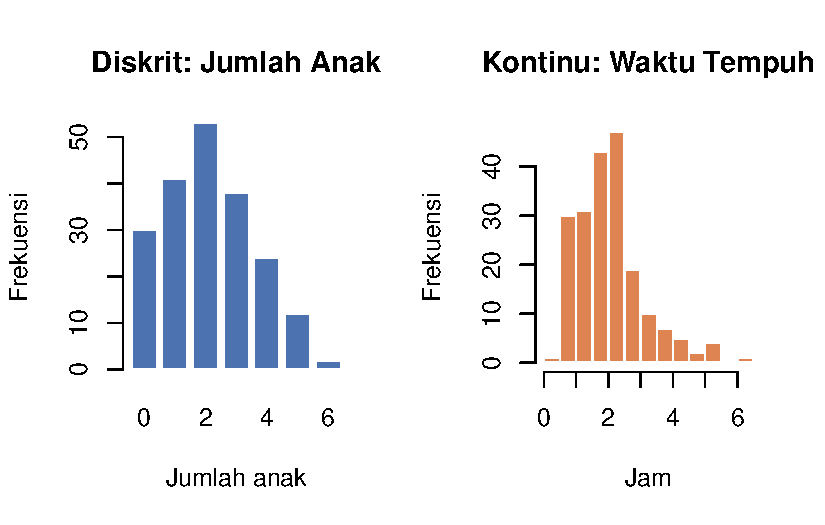
\includegraphics[keepaspectratio]{chapters/P02_files/figure-pdf/unnamed-chunk-6-1.pdf}}

\begin{Shaded}
\begin{Highlighting}[]
\FunctionTok{par}\NormalTok{(}\AttributeTok{mfrow =} \FunctionTok{c}\NormalTok{(}\DecValTok{1}\NormalTok{, }\DecValTok{1}\NormalTok{))}
\end{Highlighting}
\end{Shaded}

\subsection{Pohon Klasifikasi Data}\label{pohon-klasifikasi-data}

{\def\LTcaptype{none} % do not increment counter
\begin{longtable}[]{@{}
  >{\raggedright\arraybackslash}p{(\linewidth - 6\tabcolsep) * \real{0.2500}}
  >{\raggedright\arraybackslash}p{(\linewidth - 6\tabcolsep) * \real{0.2500}}
  >{\raggedright\arraybackslash}p{(\linewidth - 6\tabcolsep) * \real{0.2500}}
  >{\raggedright\arraybackslash}p{(\linewidth - 6\tabcolsep) * \real{0.2500}}@{}}
\toprule\noalign{}
\begin{minipage}[b]{\linewidth}\raggedright
Tingkat 1
\end{minipage} & \begin{minipage}[b]{\linewidth}\raggedright
Tingkat 2
\end{minipage} & \begin{minipage}[b]{\linewidth}\raggedright
Skala yang mungkin
\end{minipage} & \begin{minipage}[b]{\linewidth}\raggedright
Contoh
\end{minipage} \\
\midrule\noalign{}
\endhead
\bottomrule\noalign{}
\endlastfoot
Kualitatif & Tanpa urutan & Nominal & Provinsi, merek ponsel \\
Kualitatif & Berurutan & Ordinal & Tingkat pendidikan, peringkat
hotel \\
Kuantitatif & Diskrit & Rasio (umumnya) & Jumlah kunjungan \\
Kuantitatif & Kontinu & Interval atau rasio & Suhu °C (interval), berat
(rasio) \\
\end{longtable}
}

\section{Sumber Data}\label{sumber-data}

\subsection{Data Primer vs Sekunder}\label{data-primer-vs-sekunder}

{\def\LTcaptype{none} % do not increment counter
\begin{longtable}[]{@{}
  >{\raggedright\arraybackslash}p{(\linewidth - 4\tabcolsep) * \real{0.3333}}
  >{\raggedright\arraybackslash}p{(\linewidth - 4\tabcolsep) * \real{0.3333}}
  >{\raggedright\arraybackslash}p{(\linewidth - 4\tabcolsep) * \real{0.3333}}@{}}
\toprule\noalign{}
\begin{minipage}[b]{\linewidth}\raggedright
Aspek
\end{minipage} & \begin{minipage}[b]{\linewidth}\raggedright
Data Primer
\end{minipage} & \begin{minipage}[b]{\linewidth}\raggedright
Data Sekunder
\end{minipage} \\
\midrule\noalign{}
\endhead
\bottomrule\noalign{}
\endlastfoot
\textbf{Definisi} & Dikumpulkan \textbf{sendiri} oleh peneliti untuk
tujuan penelitiannya & Dikumpulkan \textbf{pihak lain} untuk tujuan
lain, lalu dipakai ulang \\
\textbf{Contoh} & Kuesioner kepuasan yang Anda sebar; pengukuran sampel
air di lapangan & Data BPS, laporan keuangan emiten, \emph{dataset}
Kaggle, log transaksi perusahaan \\
\textbf{Kelebihan} & Sesuai kebutuhan; definisi variabel dan metode
diketahui persis & Murah, cepat, sering berukuran besar dan mencakup
periode panjang \\
\textbf{Kelemahan} & Mahal, lama, butuh desain yang cermat & Definisi
variabel mungkin tidak sesuai; kualitas dan cara pengumpulan harus
diverifikasi \\
\end{longtable}
}

Dalam data science, sebagian besar pekerjaan memakai data
\textbf{sekunder} (misalnya data transaksi yang tercatat otomatis).
Karena kita tidak mengumpulkannya sendiri, \textbf{metadata} --
keterangan tentang arti tiap variabel, satuan, kode, periode, dan cara
pengumpulan -- menjadi sangat penting.

\subsection{Menjelajahi Data Sekunder di
R}\label{menjelajahi-data-sekunder-di-r}

R menyediakan banyak dataset sekunder bawaan beserta dokumentasinya.
Contohnya airquality: pengukuran kualitas udara harian di New York
(Mei--September 1973).

\begin{Shaded}
\begin{Highlighting}[]
\FunctionTok{str}\NormalTok{(airquality)}
\end{Highlighting}
\end{Shaded}

\begin{verbatim}
'data.frame':   153 obs. of  6 variables:
 $ Ozone  : int  41 36 12 18 NA 28 23 19 8 NA ...
 $ Solar.R: int  190 118 149 313 NA NA 299 99 19 194 ...
 $ Wind   : num  7.4 8 12.6 11.5 14.3 14.9 8.6 13.8 20.1 8.6 ...
 $ Temp   : int  67 72 74 62 56 66 65 59 61 69 ...
 $ Month  : int  5 5 5 5 5 5 5 5 5 5 ...
 $ Day    : int  1 2 3 4 5 6 7 8 9 10 ...
\end{verbatim}

\begin{Shaded}
\begin{Highlighting}[]
\FunctionTok{head}\NormalTok{(airquality)}
\end{Highlighting}
\end{Shaded}

\begin{verbatim}
  Ozone Solar.R Wind Temp Month Day
1    41     190  7.4   67     5   1
2    36     118  8.0   72     5   2
3    12     149 12.6   74     5   3
4    18     313 11.5   62     5   4
5    NA      NA 14.3   56     5   5
6    28      NA 14.9   66     5   6
\end{verbatim}

Tanpa membaca dokumentasi (?airquality), kita tidak tahu bahwa Ozone
diukur dalam ppb, Temp dalam \textbf{°F} (bukan °C), dan Month dikodekan
5--9 untuk Mei--September. Inilah pentingnya metadata.

\begin{Shaded}
\begin{Highlighting}[]
\NormalTok{metadata\_airquality }\OtherTok{\textless{}{-}} \FunctionTok{data.frame}\NormalTok{(}
\AttributeTok{Variabel =} \FunctionTok{names}\NormalTok{(airquality),}
\AttributeTok{Keterangan =} \FunctionTok{c}\NormalTok{(}\StringTok{"Rata{-}rata ozon 13.00{-}15.00"}\NormalTok{, }\StringTok{"Radiasi matahari 08.00{-}12.00"}\NormalTok{,}
\StringTok{"Rata{-}rata kecepatan angin 07.00{-}10.00"}\NormalTok{, }\StringTok{"Suhu maksimum harian"}\NormalTok{,}
\StringTok{"Bulan pengamatan"}\NormalTok{, }\StringTok{"Tanggal pengamatan"}\NormalTok{), }\AttributeTok{Satuan =} \FunctionTok{c}\NormalTok{(}\StringTok{"ppb"}\NormalTok{, }\StringTok{"Langley"}\NormalTok{, }\StringTok{"mil/jam"}\NormalTok{, }\StringTok{"°F"}\NormalTok{, }\StringTok{"Kode 5{-}9 (Mei{-}Sep)"}\NormalTok{, }\StringTok{"1{-}31"}\NormalTok{)}
\NormalTok{)}
\NormalTok{knitr}\SpecialCharTok{::}\FunctionTok{kable}\NormalTok{(metadata\_airquality, }\AttributeTok{caption =} \StringTok{"Kamus Data (Data Dictionary) airquality"}\NormalTok{)}
\end{Highlighting}
\end{Shaded}

\begin{longtable}[]{@{}lll@{}}
\caption{Kamus Data (Data Dictionary) airquality}\tabularnewline
\toprule\noalign{}
Variabel & Keterangan & Satuan \\
\midrule\noalign{}
\endfirsthead
\toprule\noalign{}
Variabel & Keterangan & Satuan \\
\midrule\noalign{}
\endhead
\bottomrule\noalign{}
\endlastfoot
Ozone & Rata-rata ozon 13.00-15.00 & ppb \\
Solar.R & Radiasi matahari 08.00-12.00 & Langley \\
Wind & Rata-rata kecepatan angin 07.00-10.00 & mil/jam \\
Temp & Suhu maksimum harian & °F \\
Month & Bulan pengamatan & Kode 5-9 (Mei-Sep) \\
Day & Tanggal pengamatan & 1-31 \\
\end{longtable}

\begin{Shaded}
\begin{Highlighting}[]
\FunctionTok{colSums}\NormalTok{(}\FunctionTok{is.na}\NormalTok{(airquality)) }\CommentTok{\# data sekunder sering memiliki nilai hilang (NA)}
\end{Highlighting}
\end{Shaded}

\begin{verbatim}
  Ozone Solar.R    Wind    Temp   Month     Day 
     37       7       0       0       0       0 
\end{verbatim}

\subsection{Mensimulasikan Data
Primer}\label{mensimulasikan-data-primer}

Data primer biasanya berasal dari formulir atau kuesioner yang Anda
rancang. Contoh: hasil formulir online yang diekspor ke CSV. Di sini isi
CSV kita tulis langsung sebagai teks.

\begin{Shaded}
\begin{Highlighting}[]
\NormalTok{csv\_survei }\OtherTok{\textless{}{-}} \StringTok{"responden,usia,jenis\_kelamin,pendidikan,kepuasan,pengeluaran\_bulanan}
\StringTok{R01,23,P,S1,Puas,1250000}
\StringTok{R02,31,L,SMA,Sangat Puas,980000}
\StringTok{R03,27,P,S2,Netral,2100000}
\StringTok{R04,45,L,S1,Tidak Puas,1750000}
\StringTok{R05,19,P,SMA,Puas,650000}
\StringTok{R06,38,L,D3,Sangat Tidak Puas,1400000"}
\NormalTok{survei }\OtherTok{\textless{}{-}} \FunctionTok{read.csv}\NormalTok{(}\AttributeTok{text =}\NormalTok{ csv\_survei, }\AttributeTok{stringsAsFactors =} \ConstantTok{FALSE}\NormalTok{)}
\FunctionTok{str}\NormalTok{(survei)}
\end{Highlighting}
\end{Shaded}

\begin{verbatim}
'data.frame':   6 obs. of  6 variables:
 $ responden          : chr  "R01" "R02" "R03" "R04" ...
 $ usia               : int  23 31 27 45 19 38
 $ jenis_kelamin      : chr  "P" "L" "P" "L" ...
 $ pendidikan         : chr  "S1" "SMA" "S2" "S1" ...
 $ kepuasan           : chr  "Puas" "Sangat Puas" "Netral" "Tidak Puas" ...
 $ pengeluaran_bulanan: int  1250000 980000 2100000 1750000 650000 1400000
\end{verbatim}

Perhatikan: read.csv() membaca pendidikan dan kepuasan sebagai teks
biasa (chr). R \textbf{tidak tahu} bahwa ``SMA \textless{} D3
\textless{} S1 \textless{} S2'' atau bahwa ``Puas'' lebih baik dari
``Netral''. Informasi urutan itu harus kita tambahkan -- inilah topik
bagian berikutnya.

\section{Skala Pengukuran}\label{skala-pengukuran}

{\def\LTcaptype{none} % do not increment counter
\begin{longtable}[]{@{}
  >{\raggedright\arraybackslash}p{(\linewidth - 6\tabcolsep) * \real{0.2500}}
  >{\raggedright\arraybackslash}p{(\linewidth - 6\tabcolsep) * \real{0.2500}}
  >{\raggedright\arraybackslash}p{(\linewidth - 6\tabcolsep) * \real{0.2500}}
  >{\raggedright\arraybackslash}p{(\linewidth - 6\tabcolsep) * \real{0.2500}}@{}}
\toprule\noalign{}
\begin{minipage}[b]{\linewidth}\raggedright
Skala
\end{minipage} & \begin{minipage}[b]{\linewidth}\raggedright
Sifat baru
\end{minipage} & \begin{minipage}[b]{\linewidth}\raggedright
Arti
\end{minipage} & \begin{minipage}[b]{\linewidth}\raggedright
Contoh
\end{minipage} \\
\midrule\noalign{}
\endhead
\bottomrule\noalign{}
\endlastfoot
\textbf{Nominal} & Identitas & Nilai hanya \textbf{membedakan} kategori
& Golongan darah, metode pembayaran, jenis kelamin \\
\textbf{Ordinal} & + Urutan & Kategori dapat \textbf{diurutkan}, tetapi
jarak antarkategori tidak pasti sama & Tingkat kepuasan, pendidikan
terakhir, peringkat lomba \\
\textbf{Interval} & + Jarak sama & Selisih antarnilai \textbf{bermakna
dan setara}, tetapi \textbf{nol tidak mutlak} & Suhu °C/°F, tahun
kalender, skor IQ \\
\textbf{Rasio} & + Nol mutlak & Nol berarti \textbf{``tidak ada sama
sekali''}, sehingga \textbf{perbandingan (rasio)} bermakna & Berat,
pendapatan, jumlah transaksi, suhu Kelvin \\
\end{longtable}
}

\subsection{Operasi yang Sah untuk Tiap
Skala}\label{operasi-yang-sah-untuk-tiap-skala}

{\def\LTcaptype{none} % do not increment counter
\begin{longtable}[]{@{}
  >{\raggedright\arraybackslash}p{(\linewidth - 8\tabcolsep) * \real{0.1667}}
  >{\centering\arraybackslash}p{(\linewidth - 8\tabcolsep) * \real{0.2083}}
  >{\centering\arraybackslash}p{(\linewidth - 8\tabcolsep) * \real{0.2083}}
  >{\centering\arraybackslash}p{(\linewidth - 8\tabcolsep) * \real{0.2083}}
  >{\centering\arraybackslash}p{(\linewidth - 8\tabcolsep) * \real{0.2083}}@{}}
\toprule\noalign{}
\begin{minipage}[b]{\linewidth}\raggedright
Operasi / Statistik
\end{minipage} & \begin{minipage}[b]{\linewidth}\centering
Nominal
\end{minipage} & \begin{minipage}[b]{\linewidth}\centering
Ordinal
\end{minipage} & \begin{minipage}[b]{\linewidth}\centering
Interval
\end{minipage} & \begin{minipage}[b]{\linewidth}\centering
Rasio
\end{minipage} \\
\midrule\noalign{}
\endhead
\bottomrule\noalign{}
\endlastfoot
Frekuensi, modus & Ya & Ya & Ya & Ya \\
Mengurutkan, median, persentil & Tidak & Ya & Ya & Ya \\
Penjumlahan/selisih, mean, simpangan baku & Tidak & Diperdebatkan & Ya &
Ya \\
Perbandingan ``dua kali lipat'', koefisien variasi & Tidak & Tidak &
Tidak & Ya \\
\end{longtable}
}

Tabel ini akan terus kita pakai: pada Pertemuan 5 untuk memilih ukuran
pemusatan, dan pada paruh kedua semester untuk memilih uji statistik.

\subsection{Nominal: Angka Hanya Sebagai
Label}\label{nominal-angka-hanya-sebagai-label}

Jika kategori nominal dikodekan dengan angka, R akan dengan senang hati
menghitung rata- ratanya -- dan hasilnya tidak bermakna.

\begin{Shaded}
\begin{Highlighting}[]
\CommentTok{\# Kode provinsi: 31 = DKI Jakarta, 32 = Jawa Barat, 33 = Jawa Tengah, 73 = Sulawesi Selatan}
\NormalTok{kode\_prov }\OtherTok{\textless{}{-}} \FunctionTok{c}\NormalTok{(}\DecValTok{32}\NormalTok{, }\DecValTok{32}\NormalTok{, }\DecValTok{31}\NormalTok{, }\DecValTok{73}\NormalTok{, }\DecValTok{33}\NormalTok{, }\DecValTok{32}\NormalTok{, }\DecValTok{31}\NormalTok{)}
\FunctionTok{mean}\NormalTok{(kode\_prov) }\CommentTok{\# "rata{-}rata provinsi" = 36,3 {-}\textgreater{} tidak bermakna!}
\end{Highlighting}
\end{Shaded}

\begin{verbatim}
[1] 37.71429
\end{verbatim}

\begin{Shaded}
\begin{Highlighting}[]
\CommentTok{\# Perlakukan sebagai kategori}
\NormalTok{prov }\OtherTok{\textless{}{-}} \FunctionTok{factor}\NormalTok{(kode\_prov, }\AttributeTok{levels =} \FunctionTok{c}\NormalTok{(}\DecValTok{31}\NormalTok{, }\DecValTok{32}\NormalTok{, }\DecValTok{33}\NormalTok{, }\DecValTok{73}\NormalTok{),}

\AttributeTok{labels =} \FunctionTok{c}\NormalTok{(}\StringTok{"DKI Jakarta"}\NormalTok{, }\StringTok{"Jawa Barat"}\NormalTok{, }\StringTok{"Jawa Tengah"}\NormalTok{, }\StringTok{"Sulawesi Selatan"}\NormalTok{))}

\FunctionTok{table}\NormalTok{(prov)}
\end{Highlighting}
\end{Shaded}

\begin{verbatim}
prov
     DKI Jakarta       Jawa Barat      Jawa Tengah Sulawesi Selatan 
               2                3                1                1 
\end{verbatim}

\begin{Shaded}
\begin{Highlighting}[]
\FunctionTok{names}\NormalTok{(}\FunctionTok{which.max}\NormalTok{(}\FunctionTok{table}\NormalTok{(prov))) }\CommentTok{\# modus: satu{-}satunya ukuran pusat yang sah}
\end{Highlighting}
\end{Shaded}

\begin{verbatim}
[1] "Jawa Barat"
\end{verbatim}

\subsection{Ordinal: Berurutan, Jarak Tidak
Pasti}\label{ordinal-berurutan-jarak-tidak-pasti}

Pada skala kepuasan ``Sangat Tidak Puas -- Tidak Puas -- Netral -- Puas
-- Sangat Puas'', kita tahu urutannya, tetapi \textbf{tidak} tahu apakah
jarak ``Netral ke Puas'' sama dengan jarak ``Puas ke Sangat Puas''.

\begin{Shaded}
\begin{Highlighting}[]
\NormalTok{tingkat\_puas }\OtherTok{\textless{}{-}} \FunctionTok{c}\NormalTok{(}\StringTok{"Sangat Tidak Puas"}\NormalTok{, }\StringTok{"Tidak Puas"}\NormalTok{, }\StringTok{"Netral"}\NormalTok{, }\StringTok{"Puas"}\NormalTok{, }\StringTok{"Sangat Puas"}\NormalTok{)}
\NormalTok{survei}\SpecialCharTok{$}\NormalTok{kepuasan }\OtherTok{\textless{}{-}} \FunctionTok{factor}\NormalTok{(survei}\SpecialCharTok{$}\NormalTok{kepuasan, }\AttributeTok{levels =}\NormalTok{ tingkat\_puas, }\AttributeTok{ordered =} \ConstantTok{TRUE}\NormalTok{)}
\NormalTok{survei}\SpecialCharTok{$}\NormalTok{pendidikan }\OtherTok{\textless{}{-}} \FunctionTok{factor}\NormalTok{(survei}\SpecialCharTok{$}\NormalTok{pendidikan, }\AttributeTok{levels =} \FunctionTok{c}\NormalTok{(}\StringTok{"SMA"}\NormalTok{, }\StringTok{"D3"}\NormalTok{, }\StringTok{"S1"}\NormalTok{, }\StringTok{"S2"}\NormalTok{),}

\AttributeTok{ordered =} \ConstantTok{TRUE}\NormalTok{)}

\NormalTok{survei}\SpecialCharTok{$}\NormalTok{kepuasan}
\end{Highlighting}
\end{Shaded}

\begin{verbatim}
[1] Puas              Sangat Puas       Netral            Tidak Puas       
[5] Puas              Sangat Tidak Puas
Levels: Sangat Tidak Puas < Tidak Puas < Netral < Puas < Sangat Puas
\end{verbatim}

\begin{Shaded}
\begin{Highlighting}[]
\NormalTok{survei}\SpecialCharTok{$}\NormalTok{kepuasan }\SpecialCharTok{\textgreater{}} \StringTok{"Netral"} \CommentTok{\# perbandingan urutan kini sah}
\end{Highlighting}
\end{Shaded}

\begin{verbatim}
[1]  TRUE  TRUE FALSE FALSE  TRUE FALSE
\end{verbatim}

\begin{Shaded}
\begin{Highlighting}[]
\FunctionTok{table}\NormalTok{(survei}\SpecialCharTok{$}\NormalTok{kepuasan)}
\end{Highlighting}
\end{Shaded}

\begin{verbatim}

Sangat Tidak Puas        Tidak Puas            Netral              Puas 
                1                 1                 1                 2 
      Sangat Puas 
                1 
\end{verbatim}

\begin{Shaded}
\begin{Highlighting}[]
\CommentTok{\# Median untuk data ordinal: kategori tengah setelah diurutkan.}
\CommentTok{\# Jika n genap dan dua data tengah berbeda kategori, median berada "di antara" keduanya.}
\NormalTok{median\_ordinal }\OtherTok{\textless{}{-}} \ControlFlowTok{function}\NormalTok{(x) \{}
\NormalTok{m }\OtherTok{\textless{}{-}} \FunctionTok{median}\NormalTok{(}\FunctionTok{as.integer}\NormalTok{(x), }\AttributeTok{na.rm =} \ConstantTok{TRUE}\NormalTok{)}
\ControlFlowTok{if}\NormalTok{ (m }\SpecialCharTok{==} \FunctionTok{floor}\NormalTok{(m)) }\FunctionTok{return}\NormalTok{(}\FunctionTok{levels}\NormalTok{(x)[m])}
\FunctionTok{paste}\NormalTok{(}\StringTok{"antara"}\NormalTok{, }\FunctionTok{levels}\NormalTok{(x)[}\FunctionTok{floor}\NormalTok{(m)], }\StringTok{"dan"}\NormalTok{, }\FunctionTok{levels}\NormalTok{(x)[}\FunctionTok{ceiling}\NormalTok{(m)])}
\NormalTok{\}}
\FunctionTok{sort}\NormalTok{(}\FunctionTok{as.integer}\NormalTok{(survei}\SpecialCharTok{$}\NormalTok{kepuasan)) }\CommentTok{\# posisi urutan tiap responden}
\end{Highlighting}
\end{Shaded}

\begin{verbatim}
[1] 1 2 3 4 4 5
\end{verbatim}

\begin{Shaded}
\begin{Highlighting}[]
\DocumentationTok{\#\# [1] 1 2 3 4 4 5}
\FunctionTok{median\_ordinal}\NormalTok{(survei}\SpecialCharTok{$}\NormalTok{kepuasan)}
\end{Highlighting}
\end{Shaded}

\begin{verbatim}
[1] "antara Netral dan Puas"
\end{verbatim}

\textbf{Likert: mean atau median?} Skor Likert (1--5) dari \textbf{satu
butir pertanyaan} secara ketat bersifat ordinal, sehingga median dan
modus lebih tepat. Dalam praktik, \textbf{jumlah atau rata-rata dari
banyak butir} (misalnya indeks kepuasan dari 10 pertanyaan) sering
diperlakukan sebagai data interval. Apa pun pilihannya, \textbf{nyatakan
asumsi Anda.}

\subsection{Interval: Selisih Bermakna, Rasio
Tidak}\label{interval-selisih-bermakna-rasio-tidak}

Suhu dalam °C memiliki jarak yang setara (naik dari 10 ke 20 °C sama
besarnya dengan dari 20 ke 30 °C), tetapi titik 0 °C \textbf{bukan}
``tidak ada panas'' -- hanya titik beku air yang dipilih secara
konvensi. Akibatnya, ``20 °C dua kali lebih panas dari 10 °C'' adalah
pernyataan \textbf{keliru}.

\begin{Shaded}
\begin{Highlighting}[]
\NormalTok{suhu\_c }\OtherTok{\textless{}{-}} \FunctionTok{c}\NormalTok{(}\AttributeTok{pagi =} \DecValTok{10}\NormalTok{, }\AttributeTok{siang =} \DecValTok{20}\NormalTok{)}
\NormalTok{suhu\_f }\OtherTok{\textless{}{-}}\NormalTok{ suhu\_c }\SpecialCharTok{*} \DecValTok{9} \SpecialCharTok{/} \DecValTok{5} \SpecialCharTok{+} \DecValTok{32}
\NormalTok{suhu\_k }\OtherTok{\textless{}{-}}\NormalTok{ suhu\_c }\SpecialCharTok{+} \FloatTok{273.15}
\NormalTok{knitr}\SpecialCharTok{::}\FunctionTok{kable}\NormalTok{(}\FunctionTok{data.frame}\NormalTok{(}
\AttributeTok{Satuan =} \FunctionTok{c}\NormalTok{(}\StringTok{"Celsius"}\NormalTok{, }\StringTok{"Fahrenheit"}\NormalTok{, }\StringTok{"Kelvin"}\NormalTok{),}
\AttributeTok{Pagi =} \FunctionTok{c}\NormalTok{(suhu\_c[}\StringTok{"pagi"}\NormalTok{], suhu\_f[}\StringTok{"pagi"}\NormalTok{], suhu\_k[}\StringTok{"pagi"}\NormalTok{]),}
\AttributeTok{Siang =} \FunctionTok{c}\NormalTok{(suhu\_c[}\StringTok{"siang"}\NormalTok{], suhu\_f[}\StringTok{"siang"}\NormalTok{], suhu\_k[}\StringTok{"siang"}\NormalTok{]),}
\AttributeTok{Rasio\_Siang\_per\_Pagi =} \FunctionTok{round}\NormalTok{(}\FunctionTok{c}\NormalTok{(suhu\_c[}\StringTok{"siang"}\NormalTok{] }\SpecialCharTok{/}\NormalTok{ suhu\_c[}\StringTok{"pagi"}\NormalTok{],}
\NormalTok{suhu\_f[}\StringTok{"siang"}\NormalTok{] }\SpecialCharTok{/}\NormalTok{ suhu\_f[}\StringTok{"pagi"}\NormalTok{],}
\NormalTok{suhu\_k[}\StringTok{"siang"}\NormalTok{] }\SpecialCharTok{/}\NormalTok{ suhu\_k[}\StringTok{"pagi"}\NormalTok{]), }\DecValTok{3}\NormalTok{),}

\AttributeTok{Selisih =} \FunctionTok{c}\NormalTok{(}\FunctionTok{diff}\NormalTok{(suhu\_c), }\FunctionTok{diff}\NormalTok{(suhu\_f), }\FunctionTok{diff}\NormalTok{(suhu\_k))}
\NormalTok{), }\AttributeTok{caption =} \StringTok{"Suhu yang sama dalam tiga satuan"}\NormalTok{)}
\end{Highlighting}
\end{Shaded}

\begin{longtable}[]{@{}lrrrr@{}}
\caption{Suhu yang sama dalam tiga satuan}\tabularnewline
\toprule\noalign{}
Satuan & Pagi & Siang & Rasio\_Siang\_per\_Pagi & Selisih \\
\midrule\noalign{}
\endfirsthead
\toprule\noalign{}
Satuan & Pagi & Siang & Rasio\_Siang\_per\_Pagi & Selisih \\
\midrule\noalign{}
\endhead
\bottomrule\noalign{}
\endlastfoot
Celsius & 10.00 & 20.00 & 2.000 & 10 \\
Fahrenheit & 50.00 & 68.00 & 1.360 & 18 \\
Kelvin & 283.15 & 293.15 & 1.035 & 10 \\
\end{longtable}

``Rasio'' suhu berubah-ubah tergantung satuan (2 kali dalam °C, 1,36
kali dalam °F, 1,035 kali dalam Kelvin) -- tanda bahwa rasio pada skala
interval \textbf{tidak bermakna}. Hanya Kelvin, yang nolnya mutlak, yang
merupakan skala rasio.

\subsection{Rasio: Semua Operasi Sah}\label{rasio-semua-operasi-sah}

Pada skala rasio, perbandingan \textbf{tetap sama} berapa pun satuannya.

\begin{Shaded}
\begin{Highlighting}[]
\NormalTok{berat\_kg }\OtherTok{\textless{}{-}} \FunctionTok{c}\NormalTok{(}\AttributeTok{koper\_A =} \DecValTok{10}\NormalTok{, }\AttributeTok{koper\_B =} \DecValTok{20}\NormalTok{)}
\NormalTok{berat\_lb }\OtherTok{\textless{}{-}}\NormalTok{ berat\_kg }\SpecialCharTok{*} \FloatTok{2.20462}
\FunctionTok{c}\NormalTok{(}\AttributeTok{Rasio\_kg =} \FunctionTok{unname}\NormalTok{(berat\_kg[}\StringTok{"koper\_B"}\NormalTok{] }\SpecialCharTok{/}\NormalTok{ berat\_kg[}\StringTok{"koper\_A"}\NormalTok{]),}
\AttributeTok{Rasio\_lb =} \FunctionTok{unname}\NormalTok{(berat\_lb[}\StringTok{"koper\_B"}\NormalTok{] }\SpecialCharTok{/}\NormalTok{ berat\_lb[}\StringTok{"koper\_A"}\NormalTok{]))}
\end{Highlighting}
\end{Shaded}

\begin{verbatim}
Rasio_kg Rasio_lb 
       2        2 
\end{verbatim}

Koper B \textbf{benar-benar} dua kali lebih berat dari koper A, dalam
satuan apa pun. Karena itu koefisien variasi (Pertemuan 5) hanya sah
untuk skala rasio.

\subsection{Menentukan Skala: Empat Pertanyaan
Berurutan}\label{menentukan-skala-empat-pertanyaan-berurutan}

{\def\LTcaptype{none} % do not increment counter
\begin{longtable}[]{@{}
  >{\centering\arraybackslash}p{(\linewidth - 6\tabcolsep) * \real{0.2941}}
  >{\raggedright\arraybackslash}p{(\linewidth - 6\tabcolsep) * \real{0.2353}}
  >{\raggedright\arraybackslash}p{(\linewidth - 6\tabcolsep) * \real{0.2353}}
  >{\raggedright\arraybackslash}p{(\linewidth - 6\tabcolsep) * \real{0.2353}}@{}}
\toprule\noalign{}
\begin{minipage}[b]{\linewidth}\centering
Langkah
\end{minipage} & \begin{minipage}[b]{\linewidth}\raggedright
Pertanyaan
\end{minipage} & \begin{minipage}[b]{\linewidth}\raggedright
Jika ``Tidak''
\end{minipage} & \begin{minipage}[b]{\linewidth}\raggedright
Jika ``Ya''
\end{minipage} \\
\midrule\noalign{}
\endhead
\bottomrule\noalign{}
\endlastfoot
1 & Apakah nilainya dapat diurutkan secara bermakna? & \textbf{Nominal}
& Lanjut ke 2 \\
2 & Apakah jarak antarnilai setara dan bermakna? & \textbf{Ordinal} &
Lanjut ke 3 \\
3 & Apakah nol berarti ``tidak ada sama sekali''? & \textbf{Interval} &
\textbf{Rasio} \\
\end{longtable}
}

\begin{Shaded}
\begin{Highlighting}[]
\NormalTok{tentukan\_skala }\OtherTok{\textless{}{-}} \ControlFlowTok{function}\NormalTok{(bisa\_diurutkan, jarak\_setara, nol\_mutlak) \{}
\ControlFlowTok{if}\NormalTok{ (}\SpecialCharTok{!}\NormalTok{bisa\_diurutkan) }\FunctionTok{return}\NormalTok{(}\StringTok{"Nominal"}\NormalTok{)}
\ControlFlowTok{if}\NormalTok{ (}\SpecialCharTok{!}\NormalTok{jarak\_setara) }\FunctionTok{return}\NormalTok{(}\StringTok{"Ordinal"}\NormalTok{)}
\ControlFlowTok{if}\NormalTok{ (}\SpecialCharTok{!}\NormalTok{nol\_mutlak) }\FunctionTok{return}\NormalTok{(}\StringTok{"Interval"}\NormalTok{)}
\StringTok{"Rasio"}
\NormalTok{\}}
\NormalTok{contoh }\OtherTok{\textless{}{-}} \FunctionTok{data.frame}\NormalTok{(}
\AttributeTok{Variabel =} \FunctionTok{c}\NormalTok{(}\StringTok{"Golongan darah"}\NormalTok{, }\StringTok{"Peringkat lomba"}\NormalTok{, }\StringTok{"Tahun lahir"}\NormalTok{, }\StringTok{"Jumlah Transaksi QRIS"}\NormalTok{, }\StringTok{"Kadar TSS air (mg/L)"}\NormalTok{, }\StringTok{"Ukuran baju (S/M/L/XL)"}\NormalTok{),}

\AttributeTok{urut =} \FunctionTok{c}\NormalTok{(}\ConstantTok{FALSE}\NormalTok{, }\ConstantTok{TRUE}\NormalTok{, }\ConstantTok{TRUE}\NormalTok{, }\ConstantTok{TRUE}\NormalTok{, }\ConstantTok{TRUE}\NormalTok{, }\ConstantTok{TRUE}\NormalTok{),}
\AttributeTok{jarak =} \FunctionTok{c}\NormalTok{(}\ConstantTok{FALSE}\NormalTok{, }\ConstantTok{FALSE}\NormalTok{, }\ConstantTok{TRUE}\NormalTok{, }\ConstantTok{TRUE}\NormalTok{, }\ConstantTok{TRUE}\NormalTok{, }\ConstantTok{FALSE}\NormalTok{),}
\AttributeTok{nol =} \FunctionTok{c}\NormalTok{(}\ConstantTok{FALSE}\NormalTok{, }\ConstantTok{FALSE}\NormalTok{, }\ConstantTok{FALSE}\NormalTok{, }\ConstantTok{TRUE}\NormalTok{, }\ConstantTok{TRUE}\NormalTok{, }\ConstantTok{FALSE}\NormalTok{)}
\NormalTok{)}
\NormalTok{contoh}\SpecialCharTok{$}\NormalTok{Skala }\OtherTok{\textless{}{-}} \FunctionTok{mapply}\NormalTok{(tentukan\_skala, contoh}\SpecialCharTok{$}\NormalTok{urut, contoh}\SpecialCharTok{$}\NormalTok{jarak, contoh}\SpecialCharTok{$}\NormalTok{nol)}
\NormalTok{knitr}\SpecialCharTok{::}\FunctionTok{kable}\NormalTok{(contoh, }\AttributeTok{caption =} \StringTok{"Contoh Penentuan Skala Pengukuran"}\NormalTok{)}
\end{Highlighting}
\end{Shaded}

\begin{longtable}[]{@{}lllll@{}}
\caption{Contoh Penentuan Skala Pengukuran}\tabularnewline
\toprule\noalign{}
Variabel & urut & jarak & nol & Skala \\
\midrule\noalign{}
\endfirsthead
\toprule\noalign{}
Variabel & urut & jarak & nol & Skala \\
\midrule\noalign{}
\endhead
\bottomrule\noalign{}
\endlastfoot
Golongan darah & FALSE & FALSE & FALSE & Nominal \\
Peringkat lomba & TRUE & FALSE & FALSE & Ordinal \\
Tahun lahir & TRUE & TRUE & FALSE & Interval \\
Jumlah Transaksi QRIS & TRUE & TRUE & TRUE & Rasio \\
Kadar TSS air (mg/L) & TRUE & TRUE & TRUE & Rasio \\
Ukuran baju (S/M/L/XL) & TRUE & FALSE & FALSE & Ordinal \\
\end{longtable}

\section{Skala dan Tipe Data di R}\label{skala-dan-tipe-data-di-r}

\subsection{Memetakan Skala ke Tipe
Data}\label{memetakan-skala-ke-tipe-data}

{\def\LTcaptype{none} % do not increment counter
\begin{longtable}[]{@{}
  >{\centering\arraybackslash}p{(\linewidth - 6\tabcolsep) * \real{0.2941}}
  >{\raggedright\arraybackslash}p{(\linewidth - 6\tabcolsep) * \real{0.2353}}
  >{\raggedright\arraybackslash}p{(\linewidth - 6\tabcolsep) * \real{0.2353}}
  >{\raggedright\arraybackslash}p{(\linewidth - 6\tabcolsep) * \real{0.2353}}@{}}
\toprule\noalign{}
\begin{minipage}[b]{\linewidth}\centering
Langkah
\end{minipage} & \begin{minipage}[b]{\linewidth}\raggedright
Pertanyaan
\end{minipage} & \begin{minipage}[b]{\linewidth}\raggedright
Jika ``Tidak''
\end{minipage} & \begin{minipage}[b]{\linewidth}\raggedright
Jika ``Ya''
\end{minipage} \\
\midrule\noalign{}
\endhead
\bottomrule\noalign{}
\endlastfoot
1 & Apakah nilainya dapat diurutkan secara bermakna? & \textbf{Nominal}
& Lanjut ke 2 \\
2 & Apakah jarak antarnilai setara dan bermakna? & \textbf{Ordinal} &
Lanjut ke 3 \\
3 & Apakah nol berarti ``tidak ada sama sekali''? & \textbf{Interval} &
\textbf{Rasio} \\
\end{longtable}
}

Tipe yang tepat membuat R \textbf{membantu} kita: grafik mengikuti
urutan kategori, fungsi ringkasan memilih cara yang benar, dan model
statistik memperlakukan variabel dengan semestinya.

\begin{Shaded}
\begin{Highlighting}[]
\FunctionTok{summary}\NormalTok{(survei}\SpecialCharTok{$}\NormalTok{kepuasan) }\CommentTok{\# ordered factor {-}\textgreater{} frekuensi per kategori, sesuai urutan}
\end{Highlighting}
\end{Shaded}

\begin{verbatim}
Sangat Tidak Puas        Tidak Puas            Netral              Puas 
                1                 1                 1                 2 
      Sangat Puas 
                1 
\end{verbatim}

\begin{Shaded}
\begin{Highlighting}[]
\FunctionTok{summary}\NormalTok{(survei}\SpecialCharTok{$}\NormalTok{pengeluaran\_bulanan) }\CommentTok{\# numeric {-}\textgreater{} ringkasan angka}
\end{Highlighting}
\end{Shaded}

\begin{verbatim}
   Min. 1st Qu.  Median    Mean 3rd Qu.    Max. 
 650000 1047500 1325000 1355000 1662500 2100000 
\end{verbatim}

\subsection{Urutan Level yang Keliru}\label{urutan-level-yang-keliru}

Tanpa urutan yang ditentukan, R mengurutkan kategori \textbf{menurut
abjad}, yang sering tidak logis:

\begin{Shaded}
\begin{Highlighting}[]
\NormalTok{ukuran\_baju }\OtherTok{\textless{}{-}} \FunctionTok{c}\NormalTok{(}\StringTok{"M"}\NormalTok{, }\StringTok{"L"}\NormalTok{, }\StringTok{"S"}\NormalTok{, }\StringTok{"XL"}\NormalTok{, }\StringTok{"M"}\NormalTok{, }\StringTok{"L"}\NormalTok{, }\StringTok{"M"}\NormalTok{, }\StringTok{"S"}\NormalTok{, }\StringTok{"XL"}\NormalTok{, }\StringTok{"L"}\NormalTok{, }\StringTok{"M"}\NormalTok{)}
\FunctionTok{par}\NormalTok{(}\AttributeTok{mfrow =} \FunctionTok{c}\NormalTok{(}\DecValTok{1}\NormalTok{, }\DecValTok{2}\NormalTok{))}
\FunctionTok{barplot}\NormalTok{(}\FunctionTok{table}\NormalTok{(}\FunctionTok{factor}\NormalTok{(ukuran\_baju)), }\AttributeTok{col =} \StringTok{"grey70"}\NormalTok{, }\AttributeTok{main =} \StringTok{"Urutan abjad (keliru)"}\NormalTok{)}
\FunctionTok{barplot}\NormalTok{(}\FunctionTok{table}\NormalTok{(}\FunctionTok{factor}\NormalTok{(ukuran\_baju, }\AttributeTok{levels =} \FunctionTok{c}\NormalTok{(}\StringTok{"S"}\NormalTok{, }\StringTok{"M"}\NormalTok{, }\StringTok{"L"}\NormalTok{, }\StringTok{"XL"}\NormalTok{))), }\AttributeTok{col =} \StringTok{"\#4C72B0"}\NormalTok{,}
\AttributeTok{main =} \StringTok{"Urutan logis (benar)"}\NormalTok{)}
\end{Highlighting}
\end{Shaded}

\pandocbounded{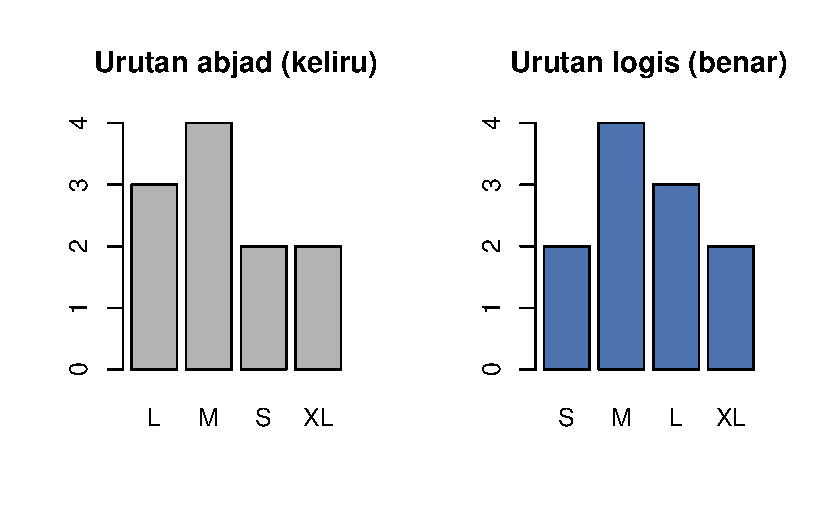
\includegraphics[keepaspectratio]{chapters/P02_files/figure-pdf/unnamed-chunk-25-1.pdf}}

\begin{Shaded}
\begin{Highlighting}[]
\FunctionTok{par}\NormalTok{(}\AttributeTok{mfrow =} \FunctionTok{c}\NormalTok{(}\DecValTok{1}\NormalTok{, }\DecValTok{1}\NormalTok{))}
\end{Highlighting}
\end{Shaded}

\subsection{Jebakan: Mengonversi Factor Berisi
Angka}\label{jebakan-mengonversi-factor-berisi-angka}

Jika sebuah factor berisi angka, as.numeric() mengembalikan
\textbf{nomor urut level}, bukan angkanya.

\begin{Shaded}
\begin{Highlighting}[]
\NormalTok{tahun }\OtherTok{\textless{}{-}} \FunctionTok{factor}\NormalTok{(}\FunctionTok{c}\NormalTok{(}\StringTok{"2021"}\NormalTok{, }\StringTok{"2023"}\NormalTok{, }\StringTok{"2021"}\NormalTok{, }\StringTok{"2024"}\NormalTok{))}
\FunctionTok{as.numeric}\NormalTok{(tahun) }\CommentTok{\# SALAH: 1 2 1 3 (nomor level)}
\end{Highlighting}
\end{Shaded}

\begin{verbatim}
[1] 1 2 1 3
\end{verbatim}

\begin{Shaded}
\begin{Highlighting}[]
\FunctionTok{as.numeric}\NormalTok{(}\FunctionTok{as.character}\NormalTok{(tahun)) }\CommentTok{\# BENAR: 2021 2023 2021 2024}
\end{Highlighting}
\end{Shaded}

\begin{verbatim}
[1] 2021 2023 2021 2024
\end{verbatim}

\subsection{Jebakan: Angka Tersimpan sebagai
Teks}\label{jebakan-angka-tersimpan-sebagai-teks}

Data dari formulir atau spreadsheet sering memuat simbol (Rp, titik
ribuan, koma desimal) sehingga terbaca sebagai teks.

\begin{Shaded}
\begin{Highlighting}[]
\NormalTok{harga\_teks }\OtherTok{\textless{}{-}} \FunctionTok{c}\NormalTok{(}\StringTok{"Rp 12.500"}\NormalTok{, }\StringTok{"Rp 8.000"}\NormalTok{, }\StringTok{"Rp 150.000"}\NormalTok{, }\StringTok{"Rp 27.250"}\NormalTok{)}
\CommentTok{\# mean(harga\_teks) akan menghasilkan NA disertai peringatan}
\NormalTok{harga }\OtherTok{\textless{}{-}} \FunctionTok{as.numeric}\NormalTok{(}\FunctionTok{gsub}\NormalTok{(}\StringTok{"[\^{}0{-}9]"}\NormalTok{, }\StringTok{""}\NormalTok{, harga\_teks)) }\CommentTok{\# buang semua karakter non{-}angka }
\NormalTok{harga}
\end{Highlighting}
\end{Shaded}

\begin{verbatim}
[1]  12500   8000 150000  27250
\end{verbatim}

\begin{Shaded}
\begin{Highlighting}[]
\FunctionTok{mean}\NormalTok{(harga)}
\end{Highlighting}
\end{Shaded}

\begin{verbatim}
[1] 49437.5
\end{verbatim}

\section{Struktur Dataset}\label{struktur-dataset}

\subsection{Observasi, Variabel, Feature, dan
Target}\label{observasi-variabel-feature-dan-target}

{\def\LTcaptype{none} % do not increment counter
\begin{longtable}[]{@{}
  >{\raggedright\arraybackslash}p{(\linewidth - 6\tabcolsep) * \real{0.2500}}
  >{\raggedright\arraybackslash}p{(\linewidth - 6\tabcolsep) * \real{0.2500}}
  >{\raggedright\arraybackslash}p{(\linewidth - 6\tabcolsep) * \real{0.2500}}
  >{\raggedright\arraybackslash}p{(\linewidth - 6\tabcolsep) * \real{0.2500}}@{}}
\toprule\noalign{}
\begin{minipage}[b]{\linewidth}\raggedright
Istilah statistika
\end{minipage} & \begin{minipage}[b]{\linewidth}\raggedright
Istilah \emph{machine learning}
\end{minipage} & \begin{minipage}[b]{\linewidth}\raggedright
Posisi dalam tabel
\end{minipage} & \begin{minipage}[b]{\linewidth}\raggedright
Contoh
\end{minipage} \\
\midrule\noalign{}
\endhead
\bottomrule\noalign{}
\endlastfoot
\textbf{Observasi} (unit observasi, kasus) & \emph{Instance},
\emph{sample}, \emph{record} & Baris & Satu bunga iris \\
\textbf{Variabel} & \emph{Attribute}, \emph{column} & Kolom & Panjang
kelopak \\
\textbf{Variabel independen} & \textbf{\emph{Feature}} (prediktor,
\(X\)) & Kolom yang dipakai untuk memprediksi & Panjang dan lebar
kelopak/mahkota \\
\textbf{Variabel dependen} & \textbf{\emph{Target}} (label, respons,
\(y\)) & Kolom yang ingin diprediksi & Spesies \\
\end{longtable}
}

\begin{Shaded}
\begin{Highlighting}[]
\FunctionTok{str}\NormalTok{(iris)}
\end{Highlighting}
\end{Shaded}

\begin{verbatim}
'data.frame':   150 obs. of  5 variables:
 $ Sepal.Length: num  5.1 4.9 4.7 4.6 5 5.4 4.6 5 4.4 4.9 ...
 $ Sepal.Width : num  3.5 3 3.2 3.1 3.6 3.9 3.4 3.4 2.9 3.1 ...
 $ Petal.Length: num  1.4 1.4 1.3 1.5 1.4 1.7 1.4 1.5 1.4 1.5 ...
 $ Petal.Width : num  0.2 0.2 0.2 0.2 0.2 0.4 0.3 0.2 0.2 0.1 ...
 $ Species     : Factor w/ 3 levels "setosa","versicolor",..: 1 1 1 1 1 1 1 1 1 1 ...
\end{verbatim}

\begin{Shaded}
\begin{Highlighting}[]
\NormalTok{X }\OtherTok{\textless{}{-}}\NormalTok{ iris[, }\FunctionTok{c}\NormalTok{(}\StringTok{"Sepal.Length"}\NormalTok{, }\StringTok{"Sepal.Width"}\NormalTok{, }\StringTok{"Petal.Length"}\NormalTok{, }\StringTok{"Petal.Width"}\NormalTok{)] }\CommentTok{\#feature}
\NormalTok{y }\OtherTok{\textless{}{-}}\NormalTok{ iris}\SpecialCharTok{$}\NormalTok{Species }\CommentTok{\#target}
\FunctionTok{dim}\NormalTok{(X) }\CommentTok{\# 150 observasi x 4 feature}
\end{Highlighting}
\end{Shaded}

\begin{verbatim}
[1] 150   4
\end{verbatim}

\begin{Shaded}
\begin{Highlighting}[]
\FunctionTok{table}\NormalTok{(y) }\CommentTok{\# target kategorik (3 kelas)}
\end{Highlighting}
\end{Shaded}

\begin{verbatim}
y
    setosa versicolor  virginica 
        50         50         50 
\end{verbatim}

\textbf{Jenis target menentukan jenis tugas:} \textbar{} Skala target
\textbar{} Tugas \textbar{} Contoh \textbar{}
\textbar:---\textbar:---\textbar:---\textbar{} \textbar{} Nominal (2
kategori) \textbar{} Klasifikasi biner \textbar{} Pelanggan \emph{churn}
atau tidak \textbar{} \textbar{} Nominal (\textgreater{} 2 kategori)
\textbar{} Klasifikasi multikelas \textbar{} Spesies iris \textbar{}
\textbar{} Ordinal \textbar{} Klasifikasi ordinal \textbar{} Tingkat
risiko kredit rendah/sedang/tinggi \textbar{} \textbar{} Interval/rasio
\textbar{} Regresi \textbar{} Harga rumah, kadar TSS \textbar{}

\subsection{Tidy Data}\label{tidy-data}

Sebuah dataset disebut tidy jika memenuhi tiga prinsip:

Setiap variabel menempati satu kolom.

Setiap observasi menempati satu baris.

Setiap nilai menempati satu sel.

Hampir semua fungsi statistika di R mengasumsikan data \emph{tidy.}

\subsection{Format Wide vs Long}\label{format-wide-vs-long}

Data yang sama dapat disusun dalam dua format. Contoh: kadar TSS (mg/L)
di tiga titik peman- tauan selama tiga bulan.

\begin{Shaded}
\begin{Highlighting}[]
\NormalTok{tss\_wide }\OtherTok{\textless{}{-}} \FunctionTok{data.frame}\NormalTok{(}
\AttributeTok{titik =} \FunctionTok{c}\NormalTok{(}\StringTok{"Hulu"}\NormalTok{, }\StringTok{"Tengah"}\NormalTok{, }\StringTok{"Hilir"}\NormalTok{),}
\AttributeTok{Jan =} \FunctionTok{c}\NormalTok{(}\DecValTok{45}\NormalTok{, }\DecValTok{120}\NormalTok{, }\DecValTok{210}\NormalTok{),}
\AttributeTok{Feb =} \FunctionTok{c}\NormalTok{(}\DecValTok{38}\NormalTok{, }\DecValTok{95}\NormalTok{, }\DecValTok{185}\NormalTok{),}
\AttributeTok{Mar =} \FunctionTok{c}\NormalTok{(}\DecValTok{52}\NormalTok{, }\DecValTok{140}\NormalTok{, }\DecValTok{260}\NormalTok{)}
\NormalTok{)}
\NormalTok{knitr}\SpecialCharTok{::}\FunctionTok{kable}\NormalTok{(tss\_wide, }\AttributeTok{caption =} \StringTok{"Format WIDE: bulan tersebar sebagai kolom"}\NormalTok{)}
\end{Highlighting}
\end{Shaded}

\begin{longtable}[]{@{}lrrr@{}}
\caption{Format WIDE: bulan tersebar sebagai kolom}\tabularnewline
\toprule\noalign{}
titik & Jan & Feb & Mar \\
\midrule\noalign{}
\endfirsthead
\toprule\noalign{}
titik & Jan & Feb & Mar \\
\midrule\noalign{}
\endhead
\bottomrule\noalign{}
\endlastfoot
Hulu & 45 & 38 & 52 \\
Tengah & 120 & 95 & 140 \\
Hilir & 210 & 185 & 260 \\
\end{longtable}

\begin{Shaded}
\begin{Highlighting}[]
\NormalTok{tss\_long }\OtherTok{\textless{}{-}} \FunctionTok{reshape}\NormalTok{(tss\_wide, }\AttributeTok{direction =} \StringTok{"long"}\NormalTok{,}

\AttributeTok{varying =} \FunctionTok{c}\NormalTok{(}\StringTok{"Jan"}\NormalTok{, }\StringTok{"Feb"}\NormalTok{, }\StringTok{"Mar"}\NormalTok{), }\AttributeTok{v.names =} \StringTok{"tss"}\NormalTok{,}
\AttributeTok{timevar =} \StringTok{"bulan"}\NormalTok{, }\AttributeTok{times =} \FunctionTok{c}\NormalTok{(}\StringTok{"Jan"}\NormalTok{, }\StringTok{"Feb"}\NormalTok{, }\StringTok{"Mar"}\NormalTok{), }\AttributeTok{idvar =} \StringTok{"titik"}\NormalTok{)}
\FunctionTok{rownames}\NormalTok{(tss\_long) }\OtherTok{\textless{}{-}} \ConstantTok{NULL}
\NormalTok{tss\_long}\SpecialCharTok{$}\NormalTok{bulan }\OtherTok{\textless{}{-}} \FunctionTok{factor}\NormalTok{(tss\_long}\SpecialCharTok{$}\NormalTok{bulan, }\AttributeTok{levels =} \FunctionTok{c}\NormalTok{(}\StringTok{"Jan"}\NormalTok{, }\StringTok{"Feb"}\NormalTok{, }\StringTok{"Mar"}\NormalTok{))}
\NormalTok{knitr}\SpecialCharTok{::}\FunctionTok{kable}\NormalTok{(tss\_long, }\AttributeTok{caption =} \StringTok{"Format LONG (tidy): satu baris = satu pengukuran"}\NormalTok{)}
\end{Highlighting}
\end{Shaded}

\begin{longtable}[]{@{}llr@{}}
\caption{Format LONG (tidy): satu baris = satu
pengukuran}\tabularnewline
\toprule\noalign{}
titik & bulan & tss \\
\midrule\noalign{}
\endfirsthead
\toprule\noalign{}
titik & bulan & tss \\
\midrule\noalign{}
\endhead
\bottomrule\noalign{}
\endlastfoot
Hulu & Jan & 45 \\
Tengah & Jan & 120 \\
Hilir & Jan & 210 \\
Hulu & Feb & 38 \\
Tengah & Feb & 95 \\
Hilir & Feb & 185 \\
Hulu & Mar & 52 \\
Tengah & Mar & 140 \\
Hilir & Mar & 260 \\
\end{longtable}

Pada format wide, satu variabel (bulan) tersembunyi di nama-nama kolom.
Format long bersifat tidy: setiap baris adalah \textbf{satu pengukuran}
(titik x bulan), sehingga mudah diringkas per kelompok:

\begin{Shaded}
\begin{Highlighting}[]
\FunctionTok{aggregate}\NormalTok{(tss }\SpecialCharTok{\textasciitilde{}}\NormalTok{ titik, }\AttributeTok{data =}\NormalTok{ tss\_long, }\AttributeTok{FUN =}\NormalTok{ mean)}
\end{Highlighting}
\end{Shaded}

\begin{verbatim}
   titik      tss
1  Hilir 218.3333
2   Hulu  45.0000
3 Tengah 118.3333
\end{verbatim}

\begin{Shaded}
\begin{Highlighting}[]
\FunctionTok{aggregate}\NormalTok{(tss }\SpecialCharTok{\textasciitilde{}}\NormalTok{ bulan, }\AttributeTok{data =}\NormalTok{ tss\_long, }\AttributeTok{FUN =}\NormalTok{ mean)}
\end{Highlighting}
\end{Shaded}

\begin{verbatim}
  bulan      tss
1   Jan 125.0000
2   Feb 106.0000
3   Mar 150.6667
\end{verbatim}

Format wide tetap berguna untuk \textbf{menyajikan} tabel kepada pembaca
manusia; format long lebih cocok untuk \textbf{analisis.}

\section{Studi Kasus Komprehensif: Membersihkan Data
Pelanggan}\label{studi-kasus-komprehensif-membersihkan-data-pelanggan}

\textbf{Konteks}: Tim analytics sebuah e-commerce menerima ekspor data
pelanggan (data \textbf{sekunder} dari sistem CRM) untuk membangun model
prediksi churn (pelanggan berhenti berlangganan). Datanya masih
``mentah''.

\begin{Shaded}
\begin{Highlighting}[]
\NormalTok{csv\_pelanggan }\OtherTok{\textless{}{-}} \StringTok{"id,gender,kota,segmen,rating\_layanan,lama\_langganan\_bln,total\_belanja,suhu\_gudang\_c,churn}
\StringTok{C001,1,Bekasi,Gold,4,26,Rp 4.250.000,24.5,Tidak}
\StringTok{C002,2,Bandung,Silver,2,5,Rp 850.000,25.1,Ya}
\StringTok{C003,2,Bekasi,Platinum,5,48,Rp 12.900.000,23.8,Tidak}
\StringTok{C004,1,Surabaya,Silver,3,12,Rp 1.320.000,26.0,Tidak}
\StringTok{C005,1,Bandung,Bronze,1,3,Rp 210.000,24.9,Ya}
\StringTok{C006,2,Medan,Gold,4,30,Rp 5.100.000,25.4,Tidak}
\StringTok{C007,1,Bekasi,Bronze,2,7,Rp 480.000,24.2,Ya}
\StringTok{C008,2,Surabaya,Platinum,5,60,Rp 15.750.000,25.7,Tidak"}
\NormalTok{pelanggan }\OtherTok{\textless{}{-}} \FunctionTok{read.csv}\NormalTok{(}\AttributeTok{text =}\NormalTok{ csv\_pelanggan, }\AttributeTok{stringsAsFactors =} \ConstantTok{FALSE}\NormalTok{)}
\FunctionTok{str}\NormalTok{(pelanggan)}
\end{Highlighting}
\end{Shaded}

\begin{verbatim}
'data.frame':   8 obs. of  9 variables:
 $ id                : chr  "C001" "C002" "C003" "C004" ...
 $ gender            : int  1 2 2 1 1 2 1 2
 $ kota              : chr  "Bekasi" "Bandung" "Bekasi" "Surabaya" ...
 $ segmen            : chr  "Gold" "Silver" "Platinum" "Silver" ...
 $ rating_layanan    : int  4 2 5 3 1 4 2 5
 $ lama_langganan_bln: int  26 5 48 12 3 30 7 60
 $ total_belanja     : chr  "Rp 4.250.000" "Rp 850.000" "Rp 12.900.000" "Rp 1.320.000" ...
 $ suhu_gudang_c     : num  24.5 25.1 23.8 26 24.9 25.4 24.2 25.7
 $ churn             : chr  "Tidak" "Ya" "Tidak" "Tidak" ...
\end{verbatim}

\textbf{Metadata dari tim CRM}: gender 1 = Laki-laki, 2 = Perempuan;
segmen berurutan Bronze \textless{} Silver \textless{} Gold \textless{}
Platinum; rating\_layanan skala 1--5 (1 = sangat buruk); suhu\_gudang\_c
= suhu rata-rata gudang pengirim (°C).

\subsection{Langkah 1: Klasifikasi Setiap
Variabel}\label{langkah-1-klasifikasi-setiap-variabel}

{\def\LTcaptype{none} % do not increment counter
\begin{longtable}[]{@{}
  >{\raggedright\arraybackslash}p{(\linewidth - 10\tabcolsep) * \real{0.1538}}
  >{\raggedright\arraybackslash}p{(\linewidth - 10\tabcolsep) * \real{0.1538}}
  >{\raggedright\arraybackslash}p{(\linewidth - 10\tabcolsep) * \real{0.1538}}
  >{\centering\arraybackslash}p{(\linewidth - 10\tabcolsep) * \real{0.1923}}
  >{\centering\arraybackslash}p{(\linewidth - 10\tabcolsep) * \real{0.1923}}
  >{\raggedright\arraybackslash}p{(\linewidth - 10\tabcolsep) * \real{0.1538}}@{}}
\toprule\noalign{}
\begin{minipage}[b]{\linewidth}\raggedright
Variabel
\end{minipage} & \begin{minipage}[b]{\linewidth}\raggedright
Jenis data
\end{minipage} & \begin{minipage}[b]{\linewidth}\raggedright
Skala
\end{minipage} & \begin{minipage}[b]{\linewidth}\centering
Tipe R saat ini
\end{minipage} & \begin{minipage}[b]{\linewidth}\centering
Tipe R seharusnya
\end{minipage} & \begin{minipage}[b]{\linewidth}\raggedright
Peran
\end{minipage} \\
\midrule\noalign{}
\endhead
\bottomrule\noalign{}
\endlastfoot
\texttt{id} & Label & \(-\) & \texttt{chr} & \texttt{character} &
Pengenal (bukan \emph{feature}) \\
\texttt{gender} & Kualitatif & Nominal & \texttt{int} & \texttt{factor}
& \emph{Feature} \\
\texttt{kota} & Kualitatif & Nominal & \texttt{chr} & \texttt{factor} &
\emph{Feature} \\
\texttt{segmen} & Kualitatif & Ordinal & \texttt{chr} & \texttt{ordered}
& \emph{Feature} \\
\texttt{rating\_layanan} & Kualitatif (berkode angka) & Ordinal &
\texttt{int} & \texttt{ordered} & \emph{Feature} \\
\texttt{lama\_langganan\_bln} & Kuantitatif kontinu (dicatat bulat) &
Rasio & \texttt{int} & \texttt{numeric} & \emph{Feature} \\
\texttt{total\_belanja} & Kuantitatif (diperlakukan kontinu) & Rasio &
\texttt{chr} & \texttt{numeric} & \emph{Feature} \\
\texttt{suhu\_gudang\_c} & Kuantitatif kontinu & Interval & \texttt{num}
& \texttt{numeric} & \emph{Feature} \\
\texttt{churn} & Kualitatif & Nominal (biner) & \texttt{chr} &
\texttt{factor} & \textbf{\emph{Target}} \\
\end{longtable}
}

\subsection{Langkah 2: Mengonversi ke Tipe yang
Tepat}\label{langkah-2-mengonversi-ke-tipe-yang-tepat}

\begin{Shaded}
\begin{Highlighting}[]
\NormalTok{bersih }\OtherTok{\textless{}{-}} \FunctionTok{within}\NormalTok{(pelanggan, \{}
\NormalTok{gender }\OtherTok{\textless{}{-}} \FunctionTok{factor}\NormalTok{(gender, }\AttributeTok{levels =} \FunctionTok{c}\NormalTok{(}\DecValTok{1}\NormalTok{, }\DecValTok{2}\NormalTok{), }\AttributeTok{labels =} \FunctionTok{c}\NormalTok{(}\StringTok{"Laki{-}laki"}\NormalTok{, }\StringTok{"Perempuan"}\NormalTok{))}
\NormalTok{kota }\OtherTok{\textless{}{-}} \FunctionTok{factor}\NormalTok{(kota)}
\NormalTok{segmen }\OtherTok{\textless{}{-}} \FunctionTok{factor}\NormalTok{(segmen, }\AttributeTok{levels =} \FunctionTok{c}\NormalTok{(}\StringTok{"Bronze"}\NormalTok{, }\StringTok{"Silver"}\NormalTok{, }\StringTok{"Gold"}\NormalTok{, }\StringTok{"Platinum"}\NormalTok{),}

\AttributeTok{ordered =} \ConstantTok{TRUE}\NormalTok{)}

\NormalTok{rating\_layanan }\OtherTok{\textless{}{-}} \FunctionTok{factor}\NormalTok{(rating\_layanan, }\AttributeTok{levels =} \DecValTok{1}\SpecialCharTok{:}\DecValTok{5}\NormalTok{, }\AttributeTok{ordered =} \ConstantTok{TRUE}\NormalTok{)}
\NormalTok{total\_belanja }\OtherTok{\textless{}{-}} \FunctionTok{as.numeric}\NormalTok{(}\FunctionTok{gsub}\NormalTok{(}\StringTok{"[\^{}0{-}9]"}\NormalTok{, }\StringTok{""}\NormalTok{, total\_belanja))}
\NormalTok{churn }\OtherTok{\textless{}{-}} \FunctionTok{factor}\NormalTok{(churn, }\AttributeTok{levels =} \FunctionTok{c}\NormalTok{(}\StringTok{"Tidak"}\NormalTok{, }\StringTok{"Ya"}\NormalTok{))}
\NormalTok{\})}
\FunctionTok{str}\NormalTok{(bersih)}
\end{Highlighting}
\end{Shaded}

\begin{verbatim}
'data.frame':   8 obs. of  9 variables:
 $ id                : chr  "C001" "C002" "C003" "C004" ...
 $ gender            : Factor w/ 2 levels "Laki-laki","Perempuan": 1 2 2 1 1 2 1 2
 $ kota              : Factor w/ 4 levels "Bandung","Bekasi",..: 2 1 2 4 1 3 2 4
 $ segmen            : Ord.factor w/ 4 levels "Bronze"<"Silver"<..: 3 2 4 2 1 3 1 4
 $ rating_layanan    : Ord.factor w/ 5 levels "1"<"2"<"3"<"4"<..: 4 2 5 3 1 4 2 5
 $ lama_langganan_bln: int  26 5 48 12 3 30 7 60
 $ total_belanja     : num  4250000 850000 12900000 1320000 210000 ...
 $ suhu_gudang_c     : num  24.5 25.1 23.8 26 24.9 25.4 24.2 25.7
 $ churn             : Factor w/ 2 levels "Tidak","Ya": 1 2 1 1 2 1 2 1
\end{verbatim}

\subsection{Langkah 3: Ringkasan yang Sesuai
Skala}\label{langkah-3-ringkasan-yang-sesuai-skala}

\begin{Shaded}
\begin{Highlighting}[]
\FunctionTok{table}\NormalTok{(bersih}\SpecialCharTok{$}\NormalTok{gender) }\CommentTok{\# nominal {-}\textgreater{} frekuensi}
\end{Highlighting}
\end{Shaded}

\begin{verbatim}

Laki-laki Perempuan 
        4         4 
\end{verbatim}

\begin{Shaded}
\begin{Highlighting}[]
\FunctionTok{table}\NormalTok{(bersih}\SpecialCharTok{$}\NormalTok{segmen) }\CommentTok{\# ordinal {-}\textgreater{} frekuensi berurutan}
\end{Highlighting}
\end{Shaded}

\begin{verbatim}

  Bronze   Silver     Gold Platinum 
       2        2        2        2 
\end{verbatim}

\begin{Shaded}
\begin{Highlighting}[]
\FunctionTok{median\_ordinal}\NormalTok{(bersih}\SpecialCharTok{$}\NormalTok{rating\_layanan) }\CommentTok{\# ordinal {-}\textgreater{} median kategori}
\end{Highlighting}
\end{Shaded}

\begin{verbatim}
[1] "antara 3 dan 4"
\end{verbatim}

\begin{Shaded}
\begin{Highlighting}[]
\FunctionTok{mean}\NormalTok{(bersih}\SpecialCharTok{$}\NormalTok{total\_belanja) }\CommentTok{\# rasio {-}\textgreater{} mean sah}
\end{Highlighting}
\end{Shaded}

\begin{verbatim}
[1] 5107500
\end{verbatim}

\begin{Shaded}
\begin{Highlighting}[]
\FunctionTok{max}\NormalTok{(bersih}\SpecialCharTok{$}\NormalTok{total\_belanja) }\SpecialCharTok{/} \FunctionTok{min}\NormalTok{(bersih}\SpecialCharTok{$}\NormalTok{total\_belanja) }\CommentTok{\# rasio {-}\textgreater{} perbandingan sah}
\end{Highlighting}
\end{Shaded}

\begin{verbatim}
[1] 75
\end{verbatim}

\begin{Shaded}
\begin{Highlighting}[]
\FunctionTok{table}\NormalTok{(bersih}\SpecialCharTok{$}\NormalTok{segmen, bersih}\SpecialCharTok{$}\NormalTok{churn) }\CommentTok{\# hubungan feature ordinal dan target}
\end{Highlighting}
\end{Shaded}

\begin{verbatim}
          
           Tidak Ya
  Bronze       0  2
  Silver       1  1
  Gold         2  0
  Platinum     2  0
\end{verbatim}

\subsection{Langkah 4: Memisahkan Feature dan
Target}\label{langkah-4-memisahkan-feature-dan-target}

\begin{Shaded}
\begin{Highlighting}[]
\NormalTok{X\_pel }\OtherTok{\textless{}{-}}\NormalTok{ bersih[, }\FunctionTok{setdiff}\NormalTok{(}\FunctionTok{names}\NormalTok{(bersih), }\FunctionTok{c}\NormalTok{(}\StringTok{"id"}\NormalTok{, }\StringTok{"churn"}\NormalTok{))]}
\NormalTok{y\_pel }\OtherTok{\textless{}{-}}\NormalTok{ bersih}\SpecialCharTok{$}\NormalTok{churn}
\FunctionTok{names}\NormalTok{(X\_pel)}
\end{Highlighting}
\end{Shaded}

\begin{verbatim}
[1] "gender"             "kota"               "segmen"            
[4] "rating_layanan"     "lama_langganan_bln" "total_belanja"     
[7] "suhu_gudang_c"     
\end{verbatim}

\begin{Shaded}
\begin{Highlighting}[]
\FunctionTok{table}\NormalTok{(y\_pel)}
\end{Highlighting}
\end{Shaded}

\begin{verbatim}
y_pel
Tidak    Ya 
    5     3 
\end{verbatim}

\subsection{Pertanyaan Diskusi dan
Jawaban}\label{pertanyaan-diskusi-dan-jawaban-1}

\textbf{1. Mengapa gender tidak boleh dibiarkan sebagai int?} Karena
angka 1 dan 2 hanya kode. Jika dibiarkan numerik, model akan menganggap
``Perempuan = 2 kali Laki-laki'' atau menghitung rata-rata gender
(misalnya 1,5) yang tidak bermakna. \textbf{2. Bolehkah kita menyatakan
``rata-rata rating layanan = 3,25''?} Secara ketat tidak, karena
rating\_layanan adalah satu butir skala ordinal -- jarak antara rating 1
ke 2 belum tentu sama dengan 4 ke 5. Laporan yang aman: median (antara 3
dan 4) dan distribusi frekuensinya. Jika mean tetap dilaporkan, nyatakan
bahwa rating diasumsikan berskala interval. \textbf{3. Mengapa rasio
``suhu gudang C003 dibanding C001'' tidak bermakna, sementara rasio
total belanja bermakna?} Suhu °C berskala interval (nol tidak mutlak),
sedangkan total belanja berskala rasio (Rp 0 be- rarti tidak berbelanja
sama sekali). Pelanggan C008 benar-benar berbelanja sekitar 75 kali
lipat pelanggan C005. \textbf{4. Mengapa id dikeluarkan dari feature?}
id unik untuk setiap pelanggan dan tidak memuat informasi perilaku.
Memasukkannya dapat membuat model ``menghafal'' pelanggan, bukan
mempelajari pola.

\section{Latihan Mandiri}\label{latihan-mandiri-1}

\subsection{Latihan Utama: Dataset
airquality}\label{latihan-utama-dataset-airquality}

Gunakan dataset bawaan airquality (data sekunder).

\subsubsection{Tugas 1: Klasifikasikan setiap
variabel}\label{tugas-1-klasifikasikan-setiap-variabel}

\textbf{Jawaban:}

{\def\LTcaptype{none} % do not increment counter
\begin{longtable}[]{@{}
  >{\raggedright\arraybackslash}p{(\linewidth - 6\tabcolsep) * \real{0.2500}}
  >{\raggedright\arraybackslash}p{(\linewidth - 6\tabcolsep) * \real{0.2500}}
  >{\raggedright\arraybackslash}p{(\linewidth - 6\tabcolsep) * \real{0.2500}}
  >{\raggedright\arraybackslash}p{(\linewidth - 6\tabcolsep) * \real{0.2500}}@{}}
\toprule\noalign{}
\begin{minipage}[b]{\linewidth}\raggedright
Variabel
\end{minipage} & \begin{minipage}[b]{\linewidth}\raggedright
Jenis
\end{minipage} & \begin{minipage}[b]{\linewidth}\raggedright
Skala
\end{minipage} & \begin{minipage}[b]{\linewidth}\raggedright
Alasan
\end{minipage} \\
\midrule\noalign{}
\endhead
\bottomrule\noalign{}
\endlastfoot
\texttt{Ozone} & Kuantitatif kontinu & Rasio & 0 ppb berarti tidak ada
ozon \\
\texttt{Solar.R} & Kuantitatif kontinu & Rasio & 0 berarti tidak ada
radiasi \\
\texttt{Wind} & Kuantitatif kontinu & Rasio & 0 mil/jam berarti tidak
ada angin \\
\texttt{Temp} & Kuantitatif kontinu & \textbf{Interval} & Suhu °F tidak
memiliki nol mutlak \\
\texttt{Month} & Kualitatif (berkode angka) & Ordinal & Bulan berurutan;
kodenya label \\
\texttt{Day} & Kualitatif (berkode angka) & Ordinal & Menunjukkan urutan
tanggal, bukan kuantitas \\
\end{longtable}
}

\subsubsection{Tugas 2: Ubah Month menjadi factor berurutan dengan label
nama
bulan}\label{tugas-2-ubah-month-menjadi-factor-berurutan-dengan-label-nama-bulan}

\begin{Shaded}
\begin{Highlighting}[]
\NormalTok{aq }\OtherTok{\textless{}{-}}\NormalTok{ airquality}
\NormalTok{aq}\SpecialCharTok{$}\NormalTok{Month }\OtherTok{\textless{}{-}} \FunctionTok{factor}\NormalTok{(aq}\SpecialCharTok{$}\NormalTok{Month, }\AttributeTok{levels =} \DecValTok{5}\SpecialCharTok{:}\DecValTok{9}\NormalTok{,}

\AttributeTok{labels =} \FunctionTok{c}\NormalTok{(}\StringTok{"Mei"}\NormalTok{, }\StringTok{"Jun"}\NormalTok{, }\StringTok{"Jul"}\NormalTok{, }\StringTok{"Agu"}\NormalTok{, }\StringTok{"Sep"}\NormalTok{), }\AttributeTok{ordered =} \ConstantTok{TRUE}\NormalTok{)}

\FunctionTok{table}\NormalTok{(aq}\SpecialCharTok{$}\NormalTok{Month)}
\end{Highlighting}
\end{Shaded}

\begin{verbatim}

Mei Jun Jul Agu Sep 
 31  30  31  31  30 
\end{verbatim}

\begin{Shaded}
\begin{Highlighting}[]
\FunctionTok{aggregate}\NormalTok{(Ozone }\SpecialCharTok{\textasciitilde{}}\NormalTok{ Month, }\AttributeTok{data =}\NormalTok{ aq, }\AttributeTok{FUN =}\NormalTok{ mean) }\CommentTok{\# baris dengan NA otomatis diabaikan}
\end{Highlighting}
\end{Shaded}

\begin{verbatim}
  Month    Ozone
1   Mei 23.61538
2   Jun 29.44444
3   Jul 59.11538
4   Agu 59.96154
5   Sep 31.44828
\end{verbatim}

\subsubsection{Tugas 4: Konversi Temp ke °C dan Kelvin, lalu jelaskan
mengapa rasio
suhu}\label{tugas-4-konversi-temp-ke-c-dan-kelvin-lalu-jelaskan-mengapa-rasio-suhu}

hanya sah pada Kelvin

\begin{Shaded}
\begin{Highlighting}[]
\NormalTok{aq}\SpecialCharTok{$}\NormalTok{Temp\_C }\OtherTok{\textless{}{-}}\NormalTok{ (aq}\SpecialCharTok{$}\NormalTok{Temp }\SpecialCharTok{{-}} \DecValTok{32}\NormalTok{) }\SpecialCharTok{*} \DecValTok{5} \SpecialCharTok{/} \DecValTok{9}
\NormalTok{aq}\SpecialCharTok{$}\NormalTok{Temp\_K }\OtherTok{\textless{}{-}}\NormalTok{ aq}\SpecialCharTok{$}\NormalTok{Temp\_C }\SpecialCharTok{+} \FloatTok{273.15}
\NormalTok{suhu\_ekstrem }\OtherTok{\textless{}{-}}\NormalTok{ aq[}\FunctionTok{c}\NormalTok{(}\FunctionTok{which.min}\NormalTok{(aq}\SpecialCharTok{$}\NormalTok{Temp), }\FunctionTok{which.max}\NormalTok{(aq}\SpecialCharTok{$}\NormalTok{Temp)), }\FunctionTok{c}\NormalTok{(}\StringTok{"Temp"}\NormalTok{, }\StringTok{"Temp\_C"}\NormalTok{, }\StringTok{"Temp\_K"}\NormalTok{)]}
\NormalTok{suhu\_ekstrem}
\end{Highlighting}
\end{Shaded}

\begin{verbatim}
    Temp   Temp_C   Temp_K
5     56 13.33333 286.4833
120   97 36.11111 309.2611
\end{verbatim}

\begin{Shaded}
\begin{Highlighting}[]
\FunctionTok{round}\NormalTok{(suhu\_ekstrem[}\DecValTok{2}\NormalTok{, ] }\SpecialCharTok{/}\NormalTok{ suhu\_ekstrem[}\DecValTok{1}\NormalTok{, ], }\DecValTok{3}\NormalTok{)}
\end{Highlighting}
\end{Shaded}

\begin{verbatim}
     Temp Temp_C Temp_K
120 1.732  2.708   1.08
\end{verbatim}

\textbf{Jawaban}: Hari terpanas ``tampak'' 1.73 kali lebih panas dalam
°F dan 2.71 kali dalam °C, tetapi hanya 1.08 kali dalam Kelvin. Hanya
Kelvin yang nolnya mutlak, sehingga hanya rasio Kelvin yang

\subsubsection{\texorpdfstring{Tugas 5: Tentukan \emph{feature} dan
\emph{target}}{Tugas 5: Tentukan feature dan target}}\label{tugas-5-tentukan-feature-dan-target}

bermakna secara fisik.

Jika tujuannya memprediksi kadar ozon dari kondisi cuaca, tentukan
feature, target, dan jenis tugasnya.

Jawaban: Target = Ozone (rasio) sehingga tugasnya regresi; feature =
Solar.R, Wind, Temp, dan Month. Day sebaiknya tidak dipakai langsung
karena hanya urutan tanggal.

\subsubsection{\texorpdfstring{Tugas 6 (Tantangan): Ubah ke format
\emph{long}}{Tugas 6 (Tantangan): Ubah ke format long}}\label{tugas-6-tantangan-ubah-ke-format-long}

Ubah kolom Ozone, Wind, dan Temp untuk 3 hari pertama menjadi format
long dengan kolom variabel dan nilai.

\begin{Shaded}
\begin{Highlighting}[]
\NormalTok{aq3 }\OtherTok{\textless{}{-}}\NormalTok{ airquality[}\DecValTok{1}\SpecialCharTok{:}\DecValTok{3}\NormalTok{, }\FunctionTok{c}\NormalTok{(}\StringTok{"Month"}\NormalTok{, }\StringTok{"Day"}\NormalTok{, }\StringTok{"Ozone"}\NormalTok{, }\StringTok{"Wind"}\NormalTok{, }\StringTok{"Temp"}\NormalTok{)]}
\NormalTok{aq3\_long }\OtherTok{\textless{}{-}} \FunctionTok{reshape}\NormalTok{(aq3, }\AttributeTok{direction =} \StringTok{"long"}\NormalTok{, }\AttributeTok{varying =} \FunctionTok{c}\NormalTok{(}\StringTok{"Ozone"}\NormalTok{, }\StringTok{"Wind"}\NormalTok{, }\StringTok{"Temp"}\NormalTok{),}

\AttributeTok{v.names =} \StringTok{"nilai"}\NormalTok{, }\AttributeTok{timevar =} \StringTok{"variabel"}\NormalTok{,}
\AttributeTok{times =} \FunctionTok{c}\NormalTok{(}\StringTok{"Ozone"}\NormalTok{, }\StringTok{"Wind"}\NormalTok{, }\StringTok{"Temp"}\NormalTok{), }\AttributeTok{idvar =} \FunctionTok{c}\NormalTok{(}\StringTok{"Month"}\NormalTok{, }\StringTok{"Day"}\NormalTok{))}

\FunctionTok{rownames}\NormalTok{(aq3\_long) }\OtherTok{\textless{}{-}} \ConstantTok{NULL}
\NormalTok{aq3\_long}
\end{Highlighting}
\end{Shaded}

\begin{verbatim}
  Month Day variabel nilai
1     5   1    Ozone  41.0
2     5   2    Ozone  36.0
3     5   3    Ozone  12.0
4     5   1     Wind   7.4
5     5   2     Wind   8.0
6     5   3     Wind  12.6
7     5   1     Temp  67.0
8     5   2     Temp  72.0
9     5   3     Temp  74.0
\end{verbatim}

\textbf{Catatan}: format long seperti ini praktis untuk visualisasi
banyak variabel sekaligus, tetapi perhatikan bahwa kolom nilai kini
mencampur satuan berbeda (ppb, mil/jam, °F) -- jangan meringkasnya
bersama-sama.

\subsection{Latihan Tambahan
(Self-Check)}\label{latihan-tambahan-self-check-1}

Kerjakan soal-soal berikut secara mandiri sebelum melihat kunci jawaban
pada komentar kode. \textbf{Soal A}. Tentukan skala pengukuran: (1)
nomor punggung pemain, (2) peringkat klasemen liga, (3) skor TOEFL, (4)
waktu lari 100 m, (5) tahun berdirinya perusahaan, (6) jumlah karyawan,
(7) tingkat keparahan gempa pada skala MMI (I--XII).

\begin{Shaded}
\begin{Highlighting}[]
\CommentTok{\# Kunci jawaban:}
\CommentTok{\# (1) Nominal (2) Ordinal (3) Interval (skor tanpa nol mutlak)}
\CommentTok{\# (4) Rasio (5) Interval (tahun 0 bukan "tidak ada waktu")}
\CommentTok{\# (6) Rasio (7) Ordinal (tingkatan intensitas, jarak tidak setara)}
\end{Highlighting}
\end{Shaded}

\textbf{Soal B}. Tentukan apakah data berikut diskrit atau kontinu: (1)
jumlah SKS yang diambil, (2) IPK, (3) volume air hujan harian, (4)
jumlah kendaraan yang melintas per jam, (5) usia dalam tahun.

\begin{Shaded}
\begin{Highlighting}[]
\CommentTok{\# Kunci jawaban:}
\CommentTok{\# (1) Diskrit (2) Kontinu (dalam rentang 0{-}4, dibulatkan 2 desimal)}
\CommentTok{\# (3) Kontinu (4) Diskrit}
\CommentTok{\# (5) Kontinu (usia terus bertambah; bilangan bulat hanya akibat pencatatan)}
\end{Highlighting}
\end{Shaded}

\textbf{Soal C}. Diberikan vektor kelas\_hotel \textless- c(``Bintang
3'', ``Bintang 5'', ``Bintang 4'', ``Bintang 3'', ``Bintang 5'',
``Bintang 3''). Ubah menjadi ordered factor, tampilkan frekuensinya
sesuai urutan, lalu tentukan medianya.

\begin{Shaded}
\begin{Highlighting}[]
\NormalTok{kelas\_hotel }\OtherTok{\textless{}{-}} \FunctionTok{c}\NormalTok{(}\StringTok{"Bintang 3"}\NormalTok{, }\StringTok{"Bintang 5"}\NormalTok{, }\StringTok{"Bintang 4"}\NormalTok{, }\StringTok{"Bintang 3"}\NormalTok{, }\StringTok{"Bintang 5"}\NormalTok{, }\StringTok{"Bintang 3"}\NormalTok{)}
\CommentTok{\# Kunci jawaban:}
\NormalTok{kelas\_hotel }\OtherTok{\textless{}{-}} \FunctionTok{factor}\NormalTok{(kelas\_hotel, }\AttributeTok{levels =} \FunctionTok{c}\NormalTok{(}\StringTok{"Bintang 3"}\NormalTok{, }\StringTok{"Bintang 4"}\NormalTok{, }\StringTok{"Bintang 5"}\NormalTok{),}

\AttributeTok{ordered =} \ConstantTok{TRUE}\NormalTok{)}

\FunctionTok{table}\NormalTok{(kelas\_hotel) }\CommentTok{\# 3, 1, 2}
\end{Highlighting}
\end{Shaded}

\begin{verbatim}
kelas_hotel
Bintang 3 Bintang 4 Bintang 5 
        3         1         2 
\end{verbatim}

\begin{Shaded}
\begin{Highlighting}[]
\FunctionTok{median\_ordinal}\NormalTok{(kelas\_hotel) }\CommentTok{\# "antara Bintang 3 dan Bintang 4"}
\end{Highlighting}
\end{Shaded}

\begin{verbatim}
[1] "antara Bintang 3 dan Bintang 4"
\end{verbatim}

\begin{Shaded}
\begin{Highlighting}[]
\CommentTok{\# Urutan kode: 1, 1, 1, 2, 3, 3 {-}\textgreater{} median = (1 + 2) / 2 = 1,5}
\CommentTok{\# Pada data ordinal berukuran genap, median bisa jatuh di antara dua kategori.}
\end{Highlighting}
\end{Shaded}

\textbf{Soal D}. Seorang analis menyatakan: ``Kota A (suhu rata-rata 30
°C) dua kali lebih panas daripada Kota B (15 °C).'' Apakah pernyataan
ini benar? Buktikan dengan R.

\begin{Shaded}
\begin{Highlighting}[]
\CommentTok{\# Kunci jawaban:}
\FunctionTok{c}\NormalTok{(}\AttributeTok{A =} \DecValTok{30}\NormalTok{, }\AttributeTok{B =} \DecValTok{15}\NormalTok{) }\SpecialCharTok{+} \FloatTok{273.15} \CommentTok{\# 303.15 K dan 288.15 K}
\end{Highlighting}
\end{Shaded}

\begin{verbatim}
     A      B 
303.15 288.15 
\end{verbatim}

\begin{Shaded}
\begin{Highlighting}[]
\NormalTok{(}\DecValTok{30} \SpecialCharTok{+} \FloatTok{273.15}\NormalTok{) }\SpecialCharTok{/}\NormalTok{ (}\DecValTok{15} \SpecialCharTok{+} \FloatTok{273.15}\NormalTok{) }\CommentTok{\# rasio sebenarnya \textasciitilde{} 1.052}
\end{Highlighting}
\end{Shaded}

\begin{verbatim}
[1] 1.052056
\end{verbatim}

\begin{Shaded}
\begin{Highlighting}[]
\CommentTok{\# Pernyataan KELIRU: °C berskala interval. Yang benar: Kota A lebih panas 15 °C daripada Kota B.}
\end{Highlighting}
\end{Shaded}

\section{Kesalahan Umum dalam Jenis Data dan Skala
Pengukuran}\label{kesalahan-umum-dalam-jenis-data-dan-skala-pengukuran}

\textbf{Menghitung mean dari kode kategori} -- misalnya ``rata-rata
gender = 1,46'' atau ``ratarata kode provinsi''

\textbf{Menganggap semua angka sebagai kuantitatif} -- nomor punggung,
kode pos, dan NIM adalah label

\textbf{Membuat pernyataan rasio pada skala interval} -- ``20 °C dua
kali lebih panas dari 10 °C''.

\textbf{Mengira pembulatan membuat data menjadi diskrit} -- usia ``21
tahun'' tetap kontinu.

\textbf{Membiarkan data ordinal sebagai teks} -- R mengurutkannya
menurut abjad sehingga grafik dan tabel menjadi tidak logis.

\textbf{Memakai as.numeric() langsung pada factor berisi angka} --
hasilnya nomor level; gunakan as.numeric(as.character(x)).

\textbf{Membiarkan angka tersimpan sebagai teks (``Rp 12.500'')} --
perhitungan menghasilkan NA.

\textbf{Memakai data sekunder tanpa membaca metadata} -- satuan (°F vs
°C) atau kode (5 = Mei) disalahartikan.

\textbf{Memasukkan kolom ID sebagai feature -- model menghafal, bukan
belajar.}

\textbf{Menganalisis data dalam format wide ketika sebuah variabel
tersembunyi di nama kolom} -- ubah ke format \emph{long} terlebih
dahulu.

\textbf{Merata-ratakan satu butir Likert tanpa menyatakan asumsi} --
laporkan median/frekuensi, atau nyatakan asumsi interval secara
eksplisit.

\section{Cheat Sheet: Fungsi R yang
Digunakan}\label{cheat-sheet-fungsi-r-yang-digunakan-1}

{\def\LTcaptype{none} % do not increment counter
\begin{longtable}[]{@{}
  >{\raggedright\arraybackslash}p{(\linewidth - 2\tabcolsep) * \real{0.5000}}
  >{\raggedright\arraybackslash}p{(\linewidth - 2\tabcolsep) * \real{0.5000}}@{}}
\toprule\noalign{}
\begin{minipage}[b]{\linewidth}\raggedright
Fungsi
\end{minipage} & \begin{minipage}[b]{\linewidth}\raggedright
Kegunaan
\end{minipage} \\
\midrule\noalign{}
\endhead
\bottomrule\noalign{}
\endlastfoot
\texttt{class(x)}, \texttt{str(df)} & Memeriksa tipe data \\
\texttt{integer\ (2L)}, \texttt{numeric} & Tipe bilangan bulat dan
desimal \\
\texttt{factor(x,\ levels,\ labels)} & Data nominal; memberi label pada
kode \\
\texttt{factor(x,\ levels,\ ordered\ =\ TRUE)} & Data ordinal \\
\texttt{levels(x)} & Melihat kategori dan urutannya \\
\texttt{as.integer(f)} & Nomor urut level sebuah factor \\
\texttt{as.numeric(as.character(f))} & Mengkonversi factor berisi angka
menjadi angka sebenarnya \\
\texttt{as.character(x)} & Mengubah menjadi teks \\
\texttt{gsub("{[}\^{}0-9{]}",\ "",\ x)} & Membuang karakter selain
angka \\
\texttt{read.csv(text\ =\ ...)} / \texttt{read.csv("file.csv")} &
Membaca data CSV \\
\texttt{is.na(x)}, \texttt{colSums(is.na(df))} & Mendeteksi dan
menghitung nilai hilang \\
\texttt{table(x)}, \texttt{prop.table(table(x))} & Frekuensi dan
proporsi \\
\texttt{within(df,\ \{...\})} & Mengubah beberapa kolom sekaligus \\
\texttt{reshape(df,\ direction\ =\ "long")} & Mengubah format
\emph{wide} menjadi \emph{long} \\
\texttt{aggregate(y\ \textasciitilde{}\ g,\ data,\ FUN)} & Ringkasan per
kelompok \\
\texttt{setdiff(a,\ b)} & Elemen \texttt{a} yang tidak ada di \texttt{b}
(memilih kolom \emph{feature}) \\
\texttt{mapply(f,\ ...)} & Menerapkan fungsi ke beberapa vektor secara
berpasangan \\
\texttt{data(nama)}, \texttt{?nama} & Memuat dataset bawaan dan membaca
dokumentasinya \\
\end{longtable}
}

\section{Glosarium Istilah}\label{glosarium-istilah-1}

{\def\LTcaptype{none} % do not increment counter
\begin{longtable}[]{@{}
  >{\raggedright\arraybackslash}p{(\linewidth - 2\tabcolsep) * \real{0.5000}}
  >{\raggedright\arraybackslash}p{(\linewidth - 2\tabcolsep) * \real{0.5000}}@{}}
\toprule\noalign{}
\begin{minipage}[b]{\linewidth}\raggedright
Istilah
\end{minipage} & \begin{minipage}[b]{\linewidth}\raggedright
Definisi Singkat
\end{minipage} \\
\midrule\noalign{}
\endhead
\bottomrule\noalign{}
\endlastfoot
\textbf{Data Kualitatif} & Data berupa label atau kategori \\
\textbf{Data Kuantitatif} & Data berupa angka hasil menghitung atau
mengukur \\
\textbf{Data Diskrit} & Data kuantitatif yang nilainya terhitung (hasil
menghitung) \\
\textbf{Data Kontinu} & Data kuantitatif yang dapat bernilai berapa pun
dalam suatu rentang (hasil mengukur) \\
\textbf{Data Primer} & Data yang dikumpulkan sendiri untuk tujuan
penelitian \\
\textbf{Data Sekunder} & Data yang dikumpulkan pihak lain dan dipakai
ulang \\
\textbf{Metadata / Kamus Data} & Keterangan arti, satuan, kode, dan
asal-usul setiap variabel \\
\textbf{Skala Nominal} & Skala yang hanya membedakan kategori \\
\textbf{Skala Ordinal} & Skala kategori yang dapat diurutkan, jarak
tidak pasti setara \\
\textbf{Skala Interval} & Skala dengan jarak setara tetapi tanpa nol
mutlak \\
\textbf{Skala Rasio} & Skala dengan jarak setara dan nol mutlak;
perbandingan bermakna \\
\textbf{Nol Mutlak} & Titik nol yang berarti ``tidak ada sama
sekali'' \\
\textbf{Factor} & Tipe data R untuk variabel kategorik \\
\textbf{Ordered Factor} & Factor yang kategorinya memiliki urutan \\
\textbf{Observasi} & Satu baris data (satu unit yang diamati) \\
\textbf{Feature} & Variabel masukan untuk memprediksi (variabel
independen) \\
\textbf{Target} & Variabel yang ingin diprediksi (variabel dependen) \\
\textbf{Tidy Data} & Data dengan satu variabel per kolom, satu observasi
per baris, satu nilai per sel \\
\textbf{Format Wide / Long} & Susunan data dengan pengukuran berulang
sebagai kolom / sebagai baris \\
\end{longtable}
}

\section{Rangkuman dan Kesimpulan}\label{rangkuman-dan-kesimpulan-1}

Data kualitatif berupa kategori; data kuantitatif berupa angka yang
bermakna secara aritmetika. Data kuantitatif dibagi menjadi diskrit
(menghitung) dan kontinu (mengukur).

Data primer dikumpulkan sendiri, data sekunder dipakai ulang. Data
sekunder wajib disertai metadata.

Skala pengukuran -- nominal, ordinal, interval, rasio -- bersifat
bertingkat. Makin tinggi skalanya, makin banyak operasi yang sah. Rasio
"dua kali lipat" hanya sah pada skala rasio.

Tipe data di R harus mencerminkan skala: factor untuk nominal, ordered
untuk ordinal, numeric untuk interval/rasio. R hanya tahu tipe
penyimpanan; maknanya ditentukan analis.

Dataset tidy menempatkan observasi di baris dan variabel di kolom. Dalam
machine learning, variabel dibagi menjadi feature dan target, dan skala
target menentukan jenis tugas (klasifikasi atau regresi).

\textbf{Jembatan ke sesi berikutnya:} setelah memahami jenis data,
Pertemuan 3 membahas \textbf{bagaimana data diperoleh} -- metode
pengumpulan data, teknik sampling probabilitas dan non-probabilitas,
serta berbagai bentuk \textbf{bias} yang dapat merusak kesimpulan.

\section{Referensi Pendukung}\label{referensi-pendukung-1}

Materi ini merangkum topik jenis data dan skala pengukuran (\emph{types
of data and levels of measurement}) yang umum dibahas pada bab awal buku
teks pengantar statistika bisnis/data science. Mahasiswa disarankan
melengkapi pemahaman dengan merujuk pada:

Modul/slide perkuliahan "Introduction to Statistics (SDT-1102)" --
Pertemuan 2: Jenis Data dan Skala Pengukuran.

Stevens, S. S. (1946). On the Theory of Scales of Measurement. Science,
103(2684), 677--680.

Wickham, H. (2014). Tidy Data. Journal of Statistical Software, 59(10).

Dokumentasi resmi R: ?factor, ?read.csv, ?reshape, ?airquality, ?iris
(dapat diakses langsung di R/RStudio).

\bookmarksetup{startatroot}

\chapter{Metode Pengumpulan Data, Sampling, dan
Bias}\label{metode-pengumpulan-data-sampling-dan-bias}

\section{Metode Pengumpulan Data}\label{metode-pengumpulan-data}

\subsection{Empat Metode Utama}\label{empat-metode-utama}

{\def\LTcaptype{none} % do not increment counter
\begin{longtable}[]{@{}
  >{\raggedright\arraybackslash}p{(\linewidth - 8\tabcolsep) * \real{0.2000}}
  >{\raggedright\arraybackslash}p{(\linewidth - 8\tabcolsep) * \real{0.2000}}
  >{\raggedright\arraybackslash}p{(\linewidth - 8\tabcolsep) * \real{0.2000}}
  >{\raggedright\arraybackslash}p{(\linewidth - 8\tabcolsep) * \real{0.2000}}
  >{\raggedright\arraybackslash}p{(\linewidth - 8\tabcolsep) * \real{0.2000}}@{}}
\toprule\noalign{}
\begin{minipage}[b]{\linewidth}\raggedright
Metode
\end{minipage} & \begin{minipage}[b]{\linewidth}\raggedright
Cara kerja
\end{minipage} & \begin{minipage}[b]{\linewidth}\raggedright
Kelebihan
\end{minipage} & \begin{minipage}[b]{\linewidth}\raggedright
Kelemahan
\end{minipage} & \begin{minipage}[b]{\linewidth}\raggedright
Contoh
\end{minipage} \\
\midrule\noalign{}
\endhead
\bottomrule\noalign{}
\endlastfoot
\textbf{Observasi} & Mencatat perilaku/kejadian secara langsung tanpa
bertanya & Data perilaku nyata, bukan pengakuan & Tidak dapat mengungkap
alasan/opini; bisa mengubah perilaku yang diamati & Menghitung kendaraan
di persimpangan; mencatat kadar TSS di titik pantau \\
\textbf{Survei} (kuesioner) & Mengajukan pertanyaan terstruktur kepada
banyak responden & Murah, cepat, menjangkau banyak orang & Rentan bias
respons dan nonrespons; kedalaman terbatas & Survei kepuasan pelanggan
\emph{online} \\
\textbf{Wawancara} & Tanya jawab langsung, terstruktur atau mendalam &
Informasi mendalam; bisa menggali alasan & Mahal, lama, sampel kecil;
rentan bias pewawancara & Wawancara tokoh masyarakat tentang dampak
proyek \\
\textbf{Eksperimen} & Peneliti \textbf{memberi perlakuan} secara acak
lalu mengukur dampaknya & Satu-satunya cara yang kuat untuk menyimpulkan
\textbf{sebab-akibat} & Tidak selalu etis atau praktis; kondisi bisa
artifisial & Uji A/B dua desain halaman \emph{checkout} \\
\end{longtable}
}

\subsection{Studi Observasional vs
Eksperimen}\label{studi-observasional-vs-eksperimen}

Perbedaan kuncinya:\textbf{siapa yang menentukan perlakuan?}

Pada \textbf{studi observasional}, subjek ``memilih sendiri''
kondisinya; peneliti hanya mencatat.

Pada \textbf{eksperimen}, peneliti \textbf{menetapkan} perlakuan secara
\textbf{acak} (\emph{random assignment}).

Mengapa pengacakan penting? Karena ia menyeimbangkan faktor-faktor lain
-- termasuk yang tidak kita ketahui -- di antara kelompok. Tanpa
pengacakan, perbedaan hasil bisa disebabkan oleh \textbf{variabel
pengganggu} (\emph{confounder}).

\textbf{Ilustrasi}: apakah mengikuti kelas tambahan (bootcamp)
meningkatkan nilai ujian? Kita simulasikan 200 mahasiswa. ``Motivasi''
memengaruhi keduanya: mahasiswa bermotivasi tinggi lebih mungkin ikut
bootcamp dan memang cenderung bernilai tinggi. Efek sebenarnya dari
bootcamp adalah +3 poin.

\begin{Shaded}
\begin{Highlighting}[]
\FunctionTok{set.seed}\NormalTok{(}\DecValTok{303}\NormalTok{)}
\NormalTok{n\_mhs }\OtherTok{\textless{}{-}} \DecValTok{200}
\NormalTok{motivasi }\OtherTok{\textless{}{-}} \FunctionTok{rnorm}\NormalTok{(n\_mhs, }\AttributeTok{mean =} \DecValTok{0}\NormalTok{, }\AttributeTok{sd =} \DecValTok{1}\NormalTok{)}
\NormalTok{efek\_bootcamp }\OtherTok{\textless{}{-}} \DecValTok{3}
\CommentTok{\# (a) Studi observasional: mahasiswa memilih sendiri ikut atau tidak}
\NormalTok{ikut\_obs }\OtherTok{\textless{}{-}} \FunctionTok{rbinom}\NormalTok{(n\_mhs, }\DecValTok{1}\NormalTok{, }\AttributeTok{prob =} \FunctionTok{plogis}\NormalTok{(}\FloatTok{1.5} \SpecialCharTok{*}\NormalTok{ motivasi))}
\NormalTok{nilai\_obs }\OtherTok{\textless{}{-}} \DecValTok{70} \SpecialCharTok{+} \DecValTok{6} \SpecialCharTok{*}\NormalTok{ motivasi }\SpecialCharTok{+}\NormalTok{ efek\_bootcamp }\SpecialCharTok{*}\NormalTok{ ikut\_obs }\SpecialCharTok{+} \FunctionTok{rnorm}\NormalTok{(n\_mhs, }\DecValTok{0}\NormalTok{, }\DecValTok{4}\NormalTok{)}
\NormalTok{beda\_obs }\OtherTok{\textless{}{-}} \FunctionTok{mean}\NormalTok{(nilai\_obs[ikut\_obs }\SpecialCharTok{==} \DecValTok{1}\NormalTok{]) }\SpecialCharTok{{-}} \FunctionTok{mean}\NormalTok{(nilai\_obs[ikut\_obs }\SpecialCharTok{==} \DecValTok{0}\NormalTok{])}

\CommentTok{\# (b) Eksperimen: peneliti mengacak siapa yang ikut}
\NormalTok{ikut\_eks }\OtherTok{\textless{}{-}} \FunctionTok{sample}\NormalTok{(}\FunctionTok{rep}\NormalTok{(}\FunctionTok{c}\NormalTok{(}\DecValTok{0}\NormalTok{, }\DecValTok{1}\NormalTok{), }\AttributeTok{each =}\NormalTok{ n\_mhs }\SpecialCharTok{/} \DecValTok{2}\NormalTok{))}
\NormalTok{nilai\_eks }\OtherTok{\textless{}{-}} \DecValTok{70} \SpecialCharTok{+} \DecValTok{6} \SpecialCharTok{*}\NormalTok{ motivasi }\SpecialCharTok{+}\NormalTok{ efek\_bootcamp }\SpecialCharTok{*}\NormalTok{ ikut\_eks }\SpecialCharTok{+} \FunctionTok{rnorm}\NormalTok{(n\_mhs, }\DecValTok{0}\NormalTok{, }\DecValTok{4}\NormalTok{)}
\NormalTok{beda\_eks }\OtherTok{\textless{}{-}} \FunctionTok{mean}\NormalTok{(nilai\_eks[ikut\_eks }\SpecialCharTok{==} \DecValTok{1}\NormalTok{]) }\SpecialCharTok{{-}} \FunctionTok{mean}\NormalTok{(nilai\_eks[ikut\_eks }\SpecialCharTok{==} \DecValTok{0}\NormalTok{])}

\NormalTok{knitr}\SpecialCharTok{::}\FunctionTok{kable}\NormalTok{(}\FunctionTok{data.frame}\NormalTok{(}
\AttributeTok{Desain =} \FunctionTok{c}\NormalTok{(}\StringTok{"Observasional (memilih sendiri)"}\NormalTok{, }\StringTok{"Eksperimen (diacak)"}\NormalTok{, }\StringTok{"Efek sebenarnya"}\NormalTok{),}
\AttributeTok{Selisih\_rata\_nilai =} \FunctionTok{round}\NormalTok{(}\FunctionTok{c}\NormalTok{(beda\_obs, beda\_eks, efek\_bootcamp), }\DecValTok{2}\NormalTok{),}
\AttributeTok{Rata\_motivasi\_ikut =} \FunctionTok{round}\NormalTok{(}\FunctionTok{c}\NormalTok{(}\FunctionTok{mean}\NormalTok{(motivasi[ikut\_obs }\SpecialCharTok{==} \DecValTok{1}\NormalTok{]), }\FunctionTok{mean}\NormalTok{(motivasi[ikut\_eks }\SpecialCharTok{==} \DecValTok{1}\NormalTok{]), }\ConstantTok{NA}\NormalTok{), }\DecValTok{2}\NormalTok{),}
\AttributeTok{Rata\_motivasi\_tidak =} \FunctionTok{round}\NormalTok{(}\FunctionTok{c}\NormalTok{(}\FunctionTok{mean}\NormalTok{(motivasi[ikut\_obs }\SpecialCharTok{==} \DecValTok{0}\NormalTok{]), }\FunctionTok{mean}\NormalTok{(motivasi[ikut\_eks }\SpecialCharTok{==} \DecValTok{0}\NormalTok{]), }\ConstantTok{NA}\NormalTok{), }\DecValTok{2}\NormalTok{)}
\NormalTok{), }\AttributeTok{caption =} \StringTok{"Studi observasional melebih{-}lebihkan efek bootcamp"}\NormalTok{)}
\end{Highlighting}
\end{Shaded}

\begin{longtable}[]{@{}
  >{\raggedright\arraybackslash}p{(\linewidth - 6\tabcolsep) * \real{0.3556}}
  >{\raggedleft\arraybackslash}p{(\linewidth - 6\tabcolsep) * \real{0.2111}}
  >{\raggedleft\arraybackslash}p{(\linewidth - 6\tabcolsep) * \real{0.2111}}
  >{\raggedleft\arraybackslash}p{(\linewidth - 6\tabcolsep) * \real{0.2222}}@{}}
\caption{Studi observasional melebih-lebihkan efek
bootcamp}\tabularnewline
\toprule\noalign{}
\begin{minipage}[b]{\linewidth}\raggedright
Desain
\end{minipage} & \begin{minipage}[b]{\linewidth}\raggedleft
Selisih\_rata\_nilai
\end{minipage} & \begin{minipage}[b]{\linewidth}\raggedleft
Rata\_motivasi\_ikut
\end{minipage} & \begin{minipage}[b]{\linewidth}\raggedleft
Rata\_motivasi\_tidak
\end{minipage} \\
\midrule\noalign{}
\endfirsthead
\toprule\noalign{}
\begin{minipage}[b]{\linewidth}\raggedright
Desain
\end{minipage} & \begin{minipage}[b]{\linewidth}\raggedleft
Selisih\_rata\_nilai
\end{minipage} & \begin{minipage}[b]{\linewidth}\raggedleft
Rata\_motivasi\_ikut
\end{minipage} & \begin{minipage}[b]{\linewidth}\raggedleft
Rata\_motivasi\_tidak
\end{minipage} \\
\midrule\noalign{}
\endhead
\bottomrule\noalign{}
\endlastfoot
Observasional (memilih sendiri) & 8.82 & 0.46 & -0.54 \\
Eksperimen (diacak) & 3.84 & 0.05 & -0.10 \\
Efek sebenarnya & 3.00 & NA & NA \\
\end{longtable}

Pada studi observasional, kelompok yang ikut bootcamp memang lebih
termotivasi sejak awal, sehingga selisih nilainya \textbf{jauh melebihi}
efek sebenarnya. Pada eksperimen, pengacakan membuat rata-rata motivasi
kedua kelompok hampir sama, sehingga selisih nilainya mendekati efek
sebenarnya (+3).

\section{Kerangka Sampel (Sampling
Frame)}\label{kerangka-sampel-sampling-frame}

\textbf{Kerangka} \textbf{sampel} adalah \textbf{daftar nyata} unit
populasi tempat sampel diambil -- misalnya daftar mahasiswa aktif,
daftar pelanggan di CRM, atau daftar desa dalam satu kabupaten.

{\def\LTcaptype{none} % do not increment counter
\begin{longtable}[]{@{}
  >{\raggedright\arraybackslash}p{(\linewidth - 4\tabcolsep) * \real{0.3333}}
  >{\raggedright\arraybackslash}p{(\linewidth - 4\tabcolsep) * \real{0.3333}}
  >{\raggedright\arraybackslash}p{(\linewidth - 4\tabcolsep) * \real{0.3333}}@{}}
\toprule\noalign{}
\begin{minipage}[b]{\linewidth}\raggedright
Kondisi
\end{minipage} & \begin{minipage}[b]{\linewidth}\raggedright
Akibat
\end{minipage} & \begin{minipage}[b]{\linewidth}\raggedright
Contoh
\end{minipage} \\
\midrule\noalign{}
\endhead
\bottomrule\noalign{}
\endlastfoot
Kerangka = populasi & Ideal & Daftar lengkap seluruh karyawan untuk
survei internal \\
Kerangka \textbf{kurang} dari populasi (\emph{undercoverage}) & Sebagian
populasi tidak mungkin terpilih & Survei telepon rumah tidak menjangkau
warga tanpa telepon rumah (\emph{Literary Digest}) \\
Kerangka memuat unit di luar populasi & Unit tak relevan terpilih &
Daftar pelanggan memuat akun yang sudah tidak aktif \\
\end{longtable}
}

Semua teknik \textbf{probability sampling} di bawah ini hanya seakurat
kerangka sampelnya.

\subsection{Populasi Simulasi}\label{populasi-simulasi}

Untuk seluruh bagian sampling, kita memakai populasi simulasi
\textbf{2.000 mahasiswa} yang tersebar di 5 fakultas dan 40 kelas
(masing-masing 50 mahasiswa). Variabel utama yang ingin kita duga adalah
\textbf{pengeluaran bulanan} (juta rupiah).

\begin{Shaded}
\begin{Highlighting}[]
\FunctionTok{set.seed}\NormalTok{(}\DecValTok{2026}\NormalTok{)}
\NormalTok{jumlah\_fak }\OtherTok{\textless{}{-}} \FunctionTok{c}\NormalTok{(}\AttributeTok{Teknik =} \DecValTok{600}\NormalTok{, }\AttributeTok{Ekonomi =} \DecValTok{500}\NormalTok{, }\AttributeTok{Sains =} \DecValTok{400}\NormalTok{, }\AttributeTok{Hukum =} \DecValTok{300}\NormalTok{, }\AttributeTok{Kedokteran =} \DecValTok{200}\NormalTok{)}
\NormalTok{rata\_fak }\OtherTok{\textless{}{-}} \FunctionTok{c}\NormalTok{(}\AttributeTok{Teknik =} \FloatTok{2.2}\NormalTok{, }\AttributeTok{Ekonomi =} \FloatTok{2.6}\NormalTok{, }\AttributeTok{Sains =} \FloatTok{2.0}\NormalTok{, }\AttributeTok{Hukum =} \FloatTok{2.8}\NormalTok{, }\AttributeTok{Kedokteran =} \FloatTok{4.0}\NormalTok{)}
\NormalTok{pop }\OtherTok{\textless{}{-}} \FunctionTok{data.frame}\NormalTok{(}\AttributeTok{id =} \DecValTok{1}\SpecialCharTok{:}\DecValTok{2000}\NormalTok{, }\AttributeTok{fakultas =} \FunctionTok{rep}\NormalTok{(}\FunctionTok{names}\NormalTok{(jumlah\_fak), jumlah\_fak))}
\NormalTok{pop}\SpecialCharTok{$}\NormalTok{kelas }\OtherTok{\textless{}{-}} \FunctionTok{paste0}\NormalTok{(}\FunctionTok{substr}\NormalTok{(pop}\SpecialCharTok{$}\NormalTok{fakultas, }\DecValTok{1}\NormalTok{, }\DecValTok{3}\NormalTok{), }\StringTok{"{-}"}\NormalTok{,}
\FunctionTok{ave}\NormalTok{(pop}\SpecialCharTok{$}\NormalTok{id, pop}\SpecialCharTok{$}\NormalTok{fakultas, }\AttributeTok{FUN =} \ControlFlowTok{function}\NormalTok{(i) }\FunctionTok{ceiling}\NormalTok{(}\FunctionTok{seq\_along}\NormalTok{(i) }\SpecialCharTok{/} \DecValTok{50}\NormalTok{)))}
\NormalTok{efek\_kelas }\OtherTok{\textless{}{-}} \FunctionTok{setNames}\NormalTok{(}\FunctionTok{rnorm}\NormalTok{(}\FunctionTok{length}\NormalTok{(}\FunctionTok{unique}\NormalTok{(pop}\SpecialCharTok{$}\NormalTok{kelas)), }\DecValTok{0}\NormalTok{, }\FloatTok{0.35}\NormalTok{), }\FunctionTok{unique}\NormalTok{(pop}\SpecialCharTok{$}\NormalTok{kelas))}
\NormalTok{pop}\SpecialCharTok{$}\NormalTok{pengeluaran }\OtherTok{\textless{}{-}} \FunctionTok{round}\NormalTok{(}\FunctionTok{pmax}\NormalTok{(}\FloatTok{0.5}\NormalTok{, rata\_fak[pop}\SpecialCharTok{$}\NormalTok{fakultas] }\SpecialCharTok{+}\NormalTok{ efek\_kelas[pop}\SpecialCharTok{$}\NormalTok{kelas] }\SpecialCharTok{+}
\FunctionTok{rnorm}\NormalTok{(}\DecValTok{2000}\NormalTok{, }\DecValTok{0}\NormalTok{, }\FloatTok{0.5}\NormalTok{)), }\DecValTok{2}\NormalTok{)}
\NormalTok{pop}\SpecialCharTok{$}\NormalTok{jam\_kerja }\OtherTok{\textless{}{-}} \FunctionTok{round}\NormalTok{(}\FunctionTok{pmax}\NormalTok{(}\DecValTok{0}\NormalTok{, }\FunctionTok{rnorm}\NormalTok{(}\DecValTok{2000}\NormalTok{, }\DecValTok{8}\NormalTok{, }\DecValTok{6}\NormalTok{))) }\CommentTok{\# jam kerja paruh waktu per minggu}
\NormalTok{N }\OtherTok{\textless{}{-}} \FunctionTok{nrow}\NormalTok{(pop)}
\NormalTok{mu\_pengeluaran }\OtherTok{\textless{}{-}} \FunctionTok{mean}\NormalTok{(pop}\SpecialCharTok{$}\NormalTok{pengeluaran) }\CommentTok{\# parameter yang ingin diduga}
\FunctionTok{head}\NormalTok{(pop)}
\end{Highlighting}
\end{Shaded}

\begin{verbatim}
  id fakultas kelas pengeluaran jam_kerja
1  1   Teknik Tek-1        1.80         0
2  2   Teknik Tek-1        2.77         5
3  3   Teknik Tek-1        1.78         5
4  4   Teknik Tek-1        2.54         6
5  5   Teknik Tek-1        1.97        14
6  6   Teknik Tek-1        3.09         5
\end{verbatim}

\begin{Shaded}
\begin{Highlighting}[]
\FunctionTok{table}\NormalTok{(pop}\SpecialCharTok{$}\NormalTok{fakultas)}
\end{Highlighting}
\end{Shaded}

\begin{verbatim}

   Ekonomi      Hukum Kedokteran      Sains     Teknik 
       500        300        200        400        600 
\end{verbatim}

\begin{Shaded}
\begin{Highlighting}[]
\FunctionTok{length}\NormalTok{(}\FunctionTok{unique}\NormalTok{(pop}\SpecialCharTok{$}\NormalTok{kelas))}
\end{Highlighting}
\end{Shaded}

\begin{verbatim}
[1] 40
\end{verbatim}

\begin{Shaded}
\begin{Highlighting}[]
\NormalTok{mu\_pengeluaran}
\end{Highlighting}
\end{Shaded}

\begin{verbatim}
[1] 2.517125
\end{verbatim}

\begin{Shaded}
\begin{Highlighting}[]
\FunctionTok{boxplot}\NormalTok{(pengeluaran }\SpecialCharTok{\textasciitilde{}} \FunctionTok{factor}\NormalTok{(fakultas, }\AttributeTok{levels =} \FunctionTok{names}\NormalTok{(jumlah\_fak)), }\AttributeTok{data =}\NormalTok{ pop,}
\AttributeTok{col =} \StringTok{"\#c6dbef"}\NormalTok{, }\AttributeTok{xlab =} \StringTok{"Fakultas"}\NormalTok{, }\AttributeTok{ylab =} \StringTok{"Pengeluaran (juta Rp/bulan)"}\NormalTok{,}
\AttributeTok{main =} \StringTok{"Pengeluaran Bulanan Berbeda Antarfakultas"}\NormalTok{)}
\FunctionTok{abline}\NormalTok{(}\AttributeTok{h =}\NormalTok{ mu\_pengeluaran, }\AttributeTok{col =} \StringTok{"firebrick"}\NormalTok{, }\AttributeTok{lwd =} \DecValTok{2}\NormalTok{, }\AttributeTok{lty =} \DecValTok{2}\NormalTok{)}
\end{Highlighting}
\end{Shaded}

\pandocbounded{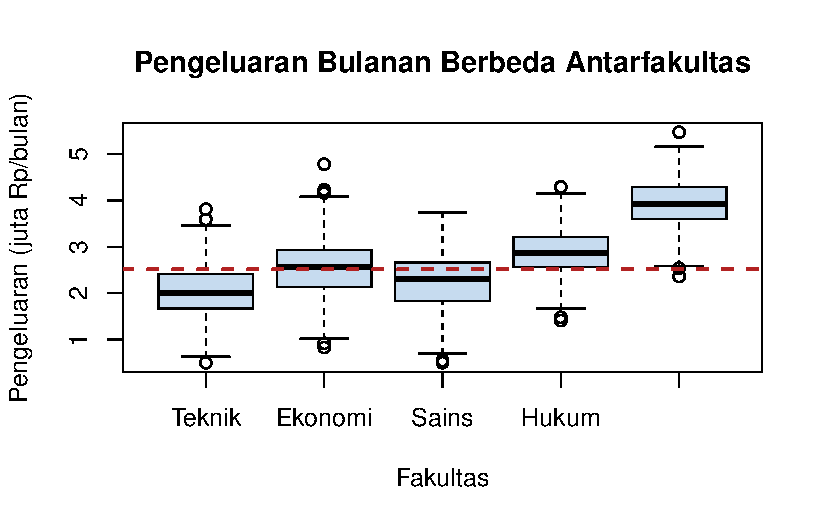
\includegraphics[keepaspectratio]{chapters/P03_files/figure-pdf/unnamed-chunk-6-1.pdf}}

Perhatikan bahwa pengeluaran \textbf{berbeda jelas antarfakultas}
(Kedokteran tertinggi). Fakta ini penting untuk memahami mengapa
sebagian teknik sampling lebih unggul dari yang lain.

\section{Probability Sampling}\label{probability-sampling}

Pada \textbf{\emph{probability sampling}}, setiap unit dalam kerangka
sampel memiliki peluang terpilih yang diketahui dan lebih dari nol, dan
pemilihannya dilakukan secara \textbf{acak.} Hanya dengan cara inilah
kita dapat mengukur ketidakpastian estimasi secara sah (dasar statistika
inferensial). Kita akan mengambil sampel berukuran \textbf{n = 100}
dengan empat teknik.

\begin{Shaded}
\begin{Highlighting}[]
\NormalTok{n }\OtherTok{\textless{}{-}} \DecValTok{100}
\end{Highlighting}
\end{Shaded}

\subsection{Simple Random Sampling
(SRS)}\label{simple-random-sampling-srs}

Setiap unit -- dan setiap kombinasi 𝑛 unit -- memiliki peluang terpilih
yang sama. Analoginya: mengundi nama dari sebuah kotak.

\begin{Shaded}
\begin{Highlighting}[]
\FunctionTok{set.seed}\NormalTok{(}\DecValTok{11}\NormalTok{)}
\NormalTok{idx\_srs }\OtherTok{\textless{}{-}} \FunctionTok{sample}\NormalTok{(}\DecValTok{1}\SpecialCharTok{:}\NormalTok{N, }\AttributeTok{size =}\NormalTok{ n) }\CommentTok{\# tanpa pengembalian}
\NormalTok{sampel\_srs }\OtherTok{\textless{}{-}}\NormalTok{ pop[idx\_srs, ]}
\FunctionTok{mean}\NormalTok{(sampel\_srs}\SpecialCharTok{$}\NormalTok{pengeluaran)}
\end{Highlighting}
\end{Shaded}

\begin{verbatim}
[1] 2.4553
\end{verbatim}

\begin{Shaded}
\begin{Highlighting}[]
\FunctionTok{table}\NormalTok{(sampel\_srs}\SpecialCharTok{$}\NormalTok{fakultas) }\CommentTok{\# komposisi fakultas terjadi secara kebetulan}
\end{Highlighting}
\end{Shaded}

\begin{verbatim}

   Ekonomi      Hukum Kedokteran      Sains     Teknik 
        19         13          8         22         38 
\end{verbatim}

\textbf{Kelebihan}: paling sederhana, dasar teori statistika. Kelemahan:
butuh kerangka lengkap; komposisi sampel bisa ``kebetulan'' tidak
seimbang (misalnya fakultas kecil kurang terwakili).

\subsection{Systematic Sampling}\label{systematic-sampling}

Pilih setiap unit ke-𝑘 dari kerangka, dengan titik awal acak:
\[k = \frac{N}{n} \quad \text{titik awal } r \sim \text{acak di antara } 1, \dots, k \quad \text{unit terpilih: } r, r+k, r+2k, \dots\]

\begin{Shaded}
\begin{Highlighting}[]
\FunctionTok{set.seed}\NormalTok{(}\DecValTok{12}\NormalTok{)}
\NormalTok{k }\OtherTok{\textless{}{-}}\NormalTok{ N }\SpecialCharTok{/}\NormalTok{ n }\CommentTok{\# interval = 20}
\NormalTok{r }\OtherTok{\textless{}{-}} \FunctionTok{sample}\NormalTok{(}\DecValTok{1}\SpecialCharTok{:}\NormalTok{k, }\DecValTok{1}\NormalTok{) }\CommentTok{\# titik awal acak}
\NormalTok{idx\_sis }\OtherTok{\textless{}{-}} \FunctionTok{seq}\NormalTok{(}\AttributeTok{from =}\NormalTok{ r, }\AttributeTok{by =}\NormalTok{ k, }\AttributeTok{length.out =}\NormalTok{ n)}
\FunctionTok{head}\NormalTok{(idx\_sis, }\DecValTok{10}\NormalTok{)}
\end{Highlighting}
\end{Shaded}

\begin{verbatim}
 [1]   2  22  42  62  82 102 122 142 162 182
\end{verbatim}

\begin{Shaded}
\begin{Highlighting}[]
\NormalTok{sampel\_sis }\OtherTok{\textless{}{-}}\NormalTok{ pop[idx\_sis, ]}
\FunctionTok{mean}\NormalTok{(sampel\_sis}\SpecialCharTok{$}\NormalTok{pengeluaran)}
\end{Highlighting}
\end{Shaded}

\begin{verbatim}
[1] 2.4928
\end{verbatim}

\begin{Shaded}
\begin{Highlighting}[]
\FunctionTok{table}\NormalTok{(sampel\_sis}\SpecialCharTok{$}\NormalTok{fakultas)}
\end{Highlighting}
\end{Shaded}

\begin{verbatim}

   Ekonomi      Hukum Kedokteran      Sains     Teknik 
        25         15         10         20         30 
\end{verbatim}

Karena kerangka kita \textbf{terurut menurut fakultas}, \emph{systematic
sampling} otomatis menyebar ke semua fakultas secara proporsional --
mirip \emph{stratified sampling}

\textbf{Bahaya periodisitas}. Jika kerangka memiliki pola berulang yang
kebetulan sama dengan interval 𝑘 (misalnya daftar transaksi harian yang
dipilih setiap 7 hari -- selalu jatuh di hari yang sama), sampel
sistematik akan \emph{bias.} Periksa urutan kerangka sebelum memakai
teknik ini.

\subsection{Stratified Sampling}\label{stratified-sampling}

Populasi dibagi menjadi kelompok \textbf{homogen} yang disebut
\textbf{strata} (di sini: fakultas), lalu diambil SRS \textbf{dari
setiap strata}. Dengan \textbf{alokasi proporsional}, ukuran sampel tiap
strata sebanding dengan ukurannya di populasi:

\[n_h = n \times \frac{N_h}{N}\]

\begin{Shaded}
\begin{Highlighting}[]
\NormalTok{alokasi }\OtherTok{\textless{}{-}} \FunctionTok{round}\NormalTok{(n }\SpecialCharTok{*}\NormalTok{ jumlah\_fak }\SpecialCharTok{/}\NormalTok{ N)}
\NormalTok{alokasi}
\end{Highlighting}
\end{Shaded}

\begin{verbatim}
    Teknik    Ekonomi      Sains      Hukum Kedokteran 
        30         25         20         15         10 
\end{verbatim}

\begin{Shaded}
\begin{Highlighting}[]
\FunctionTok{set.seed}\NormalTok{(}\DecValTok{13}\NormalTok{)}
\NormalTok{idx\_str }\OtherTok{\textless{}{-}} \FunctionTok{unlist}\NormalTok{(}\FunctionTok{lapply}\NormalTok{(}\FunctionTok{names}\NormalTok{(alokasi), }\ControlFlowTok{function}\NormalTok{(f)}
\FunctionTok{sample}\NormalTok{(}\FunctionTok{which}\NormalTok{(pop}\SpecialCharTok{$}\NormalTok{fakultas }\SpecialCharTok{==}\NormalTok{ f), alokasi[[f]])))}
\NormalTok{sampel\_str }\OtherTok{\textless{}{-}}\NormalTok{ pop[idx\_str, ]}
\FunctionTok{table}\NormalTok{(sampel\_str}\SpecialCharTok{$}\NormalTok{fakultas) }\CommentTok{\# komposisi DIJAMIN sesuai populasi}
\end{Highlighting}
\end{Shaded}

\begin{verbatim}

   Ekonomi      Hukum Kedokteran      Sains     Teknik 
        25         15         10         20         30 
\end{verbatim}

\begin{Shaded}
\begin{Highlighting}[]
\FunctionTok{mean}\NormalTok{(sampel\_str}\SpecialCharTok{$}\NormalTok{pengeluaran)}
\end{Highlighting}
\end{Shaded}

\begin{verbatim}
[1] 2.4458
\end{verbatim}

\textbf{Kelebihan}: menjamin setiap strata terwakili dan -- jika strata
berbeda satu sama lain -- lebih presisi daripada SRS.
\textbf{Kelemahan}: butuh informasi strata untuk seluruh kerangka.

\subsection{Cluster Sampling}\label{cluster-sampling}

Populasi dibagi menjadi kelompok alami yang disebut klaster (di sini:
kelas). Beberapa klaster dipilih secara acak, lalu semua anggota klaster
terpilih diamati.

\begin{Shaded}
\begin{Highlighting}[]
\FunctionTok{set.seed}\NormalTok{(}\DecValTok{14}\NormalTok{)}
\NormalTok{kelas\_terpilih }\OtherTok{\textless{}{-}} \FunctionTok{sample}\NormalTok{(}\FunctionTok{unique}\NormalTok{(pop}\SpecialCharTok{$}\NormalTok{kelas), }\AttributeTok{size =} \DecValTok{2}\NormalTok{) }\CommentTok{\# 2 kelas x 50 = 100 mahasiswa}
\NormalTok{kelas\_terpilih}
\end{Highlighting}
\end{Shaded}

\begin{verbatim}
[1] "Tek-9" "Ked-4"
\end{verbatim}

\begin{Shaded}
\begin{Highlighting}[]
\NormalTok{sampel\_klas }\OtherTok{\textless{}{-}}\NormalTok{ pop[pop}\SpecialCharTok{$}\NormalTok{kelas }\SpecialCharTok{\%in\%}\NormalTok{ kelas\_terpilih, ]}
\FunctionTok{nrow}\NormalTok{(sampel\_klas)}
\end{Highlighting}
\end{Shaded}

\begin{verbatim}
[1] 100
\end{verbatim}

\begin{Shaded}
\begin{Highlighting}[]
\FunctionTok{mean}\NormalTok{(sampel\_klas}\SpecialCharTok{$}\NormalTok{pengeluaran)}
\end{Highlighting}
\end{Shaded}

\begin{verbatim}
[1] 3.051
\end{verbatim}

\begin{Shaded}
\begin{Highlighting}[]
\FunctionTok{table}\NormalTok{(sampel\_klas}\SpecialCharTok{$}\NormalTok{fakultas)}
\end{Highlighting}
\end{Shaded}

\begin{verbatim}

Kedokteran     Teknik 
        50         50 
\end{verbatim}

\textbf{Kelebihan}: murah dan praktis -- cukup mendatangi 2 kelas, tanpa
perlu daftar seluruh mahasiswa. \textbf{Kelemahan}: anggota satu klaster
cenderung mirip satu sama lain, sehingga 100 mahasiswa dari 2 kelas
membawa informasi lebih sedikit daripada 100 mahasiswa yang dipilih acak
dari seluruh kampus (presisi lebih rendah).

\subsection{Stratified vs Cluster: Jangan
Tertukar}\label{stratified-vs-cluster-jangan-tertukar}

{\def\LTcaptype{none} % do not increment counter
\begin{longtable}[]{@{}
  >{\raggedright\arraybackslash}p{(\linewidth - 4\tabcolsep) * \real{0.3333}}
  >{\raggedright\arraybackslash}p{(\linewidth - 4\tabcolsep) * \real{0.3333}}
  >{\raggedright\arraybackslash}p{(\linewidth - 4\tabcolsep) * \real{0.3333}}@{}}
\toprule\noalign{}
\begin{minipage}[b]{\linewidth}\raggedright
Aspek
\end{minipage} & \begin{minipage}[b]{\linewidth}\raggedright
\emph{Stratified}
\end{minipage} & \begin{minipage}[b]{\linewidth}\raggedright
\emph{Cluster}
\end{minipage} \\
\midrule\noalign{}
\endhead
\bottomrule\noalign{}
\endlastfoot
Kelompok yang dibentuk & Strata: \textbf{homogen di dalam}, berbeda
antarstrata & Klaster: idealnya \textbf{heterogen di dalam} (miniatur
populasi) \\
Yang diacak & \textbf{Unit} di dalam \textbf{setiap} strata &
\textbf{Klaster-nya}; semua unit klaster terpilih diamati \\
Semua kelompok terwakili? & \textbf{Ya} & Tidak, hanya klaster
terpilih \\
Tujuan utama & Meningkatkan presisi dan keterwakilan & Menghemat biaya
dan waktu \\
\end{longtable}
}

\section{Non-probability Sampling}\label{non-probability-sampling}

Pada \textbf{\emph{non-probability}} sampling, unit dipilih
\textbf{tidak secara acak} -- berdasarkan kemudahan, pertimbangan
peneliti, atau kuota. Peluang terpilih setiap unit tidak diketahui,
sehingga ketidakpastian estimasi \textbf{tidak dapat diukur secara sah}
dan hasilnya berisiko bias.

{\def\LTcaptype{none} % do not increment counter
\begin{longtable}[]{@{}
  >{\raggedright\arraybackslash}p{(\linewidth - 6\tabcolsep) * \real{0.2500}}
  >{\raggedright\arraybackslash}p{(\linewidth - 6\tabcolsep) * \real{0.2500}}
  >{\raggedright\arraybackslash}p{(\linewidth - 6\tabcolsep) * \real{0.2500}}
  >{\raggedright\arraybackslash}p{(\linewidth - 6\tabcolsep) * \real{0.2500}}@{}}
\toprule\noalign{}
\begin{minipage}[b]{\linewidth}\raggedright
Teknik
\end{minipage} & \begin{minipage}[b]{\linewidth}\raggedright
Cara memilih
\end{minipage} & \begin{minipage}[b]{\linewidth}\raggedright
Kapan wajar dipakai
\end{minipage} & \begin{minipage}[b]{\linewidth}\raggedright
Risiko
\end{minipage} \\
\midrule\noalign{}
\endhead
\bottomrule\noalign{}
\endlastfoot
\textbf{\emph{Convenience}} & Siapa saja yang \textbf{mudah
dijangkau}{[}cite: 30{]} & Uji coba kuesioner (\emph{pilot}), eksplorasi
awal{[}cite: 30{]} & Hanya mewakili kelompok yang mudah
dijangkau{[}cite: 30{]} \\
\textbf{\emph{Purposive}} (\emph{judgmental}){[}cite: 30{]} & Dipilih
berdasarkan \textbf{pertimbangan/kriteria} peneliti{[}cite: 30{]} &
Mewawancarai ahli atau informan kunci{[}cite: 30{]} & Bergantung
penilaian subjektif peneliti{[}cite: 30{]} \\
\textbf{\emph{Quota}} & Memenuhi \textbf{kuota} per kelompok, tetapi
pemilihan di dalam kelompok tidak acak{[}cite: 30{]} & Survei cepat
dengan anggaran terbatas{[}cite: 30{]} & Komposisi tampak mewakili,
tetapi bias di dalam kelompok tetap ada{[}cite: 30{]} \\
\end{longtable}
}

Kita simulasikan bahwa convenience sampling dilakukan di \textbf{kantin
kampus}. Mahasiswa berpengeluaran tinggi lebih sering jajan di kantin,
sehingga \textbf{lebih mudah dijangkau}.

\begin{Shaded}
\begin{Highlighting}[]
\NormalTok{pop}\SpecialCharTok{$}\NormalTok{peluang\_kantin }\OtherTok{\textless{}{-}} \FunctionTok{plogis}\NormalTok{(}\SpecialCharTok{{-}}\DecValTok{3} \SpecialCharTok{+} \FloatTok{1.1} \SpecialCharTok{*}\NormalTok{ pop}\SpecialCharTok{$}\NormalTok{pengeluaran) }\CommentTok{\# makin besar pengeluaran, makin sering ke kantin}
\FunctionTok{round}\NormalTok{(}\FunctionTok{tapply}\NormalTok{(pop}\SpecialCharTok{$}\NormalTok{peluang\_kantin, pop}\SpecialCharTok{$}\NormalTok{fakultas, mean)[}\FunctionTok{names}\NormalTok{(jumlah\_fak)], }\DecValTok{2}\NormalTok{)}
\end{Highlighting}
\end{Shaded}

\begin{verbatim}
    Teknik    Ekonomi      Sains      Hukum Kedokteran 
      0.33       0.45       0.38       0.54       0.78 
\end{verbatim}

\begin{Shaded}
\begin{Highlighting}[]
\FunctionTok{set.seed}\NormalTok{(}\DecValTok{15}\NormalTok{)}
\CommentTok{\# Convenience: yang kebetulan ada di kantin}
\NormalTok{idx\_conv }\OtherTok{\textless{}{-}} \FunctionTok{sample}\NormalTok{(}\DecValTok{1}\SpecialCharTok{:}\NormalTok{N, n, }\AttributeTok{prob =}\NormalTok{ pop}\SpecialCharTok{$}\NormalTok{peluang\_kantin)}
\CommentTok{\# Purposive: peneliti memilih hanya mahasiswa Teknik ("karena paling aktif berorganisasi")}
\NormalTok{idx\_purp }\OtherTok{\textless{}{-}} \FunctionTok{sample}\NormalTok{(}\FunctionTok{which}\NormalTok{(pop}\SpecialCharTok{$}\NormalTok{fakultas }\SpecialCharTok{==} \StringTok{"Teknik"}\NormalTok{), n)}
\CommentTok{\# Quota: kuota per fakultas proporsional, tetapi diisi dengan siapa yang ada di kantin}
\NormalTok{idx\_quota }\OtherTok{\textless{}{-}} \FunctionTok{unlist}\NormalTok{(}\FunctionTok{lapply}\NormalTok{(}\FunctionTok{names}\NormalTok{(alokasi), }\ControlFlowTok{function}\NormalTok{(f) \{}
\NormalTok{kandidat }\OtherTok{\textless{}{-}} \FunctionTok{which}\NormalTok{(pop}\SpecialCharTok{$}\NormalTok{fakultas }\SpecialCharTok{==}\NormalTok{ f)}
\FunctionTok{sample}\NormalTok{(kandidat, alokasi[[f]], }\AttributeTok{prob =}\NormalTok{ pop}\SpecialCharTok{$}\NormalTok{peluang\_kantin[kandidat])}
\NormalTok{\}))}
\NormalTok{knitr}\SpecialCharTok{::}\FunctionTok{kable}\NormalTok{(}\FunctionTok{data.frame}\NormalTok{(}
\AttributeTok{Teknik =} \FunctionTok{c}\NormalTok{(}\StringTok{"Parameter (populasi)"}\NormalTok{, }\StringTok{"Convenience"}\NormalTok{, }\StringTok{"Purposive"}\NormalTok{, }\StringTok{"Quota"}\NormalTok{),}
\AttributeTok{Rata\_pengeluaran =} \FunctionTok{round}\NormalTok{(}\FunctionTok{c}\NormalTok{(mu\_pengeluaran, }\FunctionTok{mean}\NormalTok{(pop}\SpecialCharTok{$}\NormalTok{pengeluaran[idx\_conv]),}
\FunctionTok{mean}\NormalTok{(pop}\SpecialCharTok{$}\NormalTok{pengeluaran[idx\_purp]),}
\FunctionTok{mean}\NormalTok{(pop}\SpecialCharTok{$}\NormalTok{pengeluaran[idx\_quota])), }\DecValTok{3}\NormalTok{)}
\NormalTok{), }\AttributeTok{caption =} \StringTok{"Estimasi rata{-}rata pengeluaran dari sampel non{-}probabilitas (n = 100)"}\NormalTok{)}
\end{Highlighting}
\end{Shaded}

\begin{longtable}[]{@{}lr@{}}
\caption{Estimasi rata-rata pengeluaran dari sampel non-probabilitas (n
= 100)}\tabularnewline
\toprule\noalign{}
Teknik & Rata\_pengeluaran \\
\midrule\noalign{}
\endfirsthead
\toprule\noalign{}
Teknik & Rata\_pengeluaran \\
\midrule\noalign{}
\endhead
\bottomrule\noalign{}
\endlastfoot
Parameter (populasi) & 2.517 \\
Convenience & 2.657 \\
Purposive & 1.989 \\
Quota & 2.703 \\
\end{longtable}

\emph{Convenience} dan \emph{quota sampling} \textbf{melebih-lebihkan}
pengeluaran (mahasiswa kantin lebih boros), sedangkan \emph{purposive}
sampling hanya menggambarkan mahasiswa Teknik. Perhatikan bahwa
\emph{quota sampling} sudah memiliki komposisi fakultas yang ``benar'',
tetapi tetap bias karena \textbf{di dalam} setiap fakultas yang terpilih
adalah pengunjung kantin.

\section{Simulasi: Membandingkan Akurasi dan
Presisi}\label{simulasi-membandingkan-akurasi-dan-presisi}

Satu sampel bisa saja ``beruntung'' atau ``sial''. Untuk menilai sebuah
teknik secara adil, kita ulangi setiap teknik \textbf{1.000} kali dan
melihat sebaran estimasinya.

\begin{itemize}
\tightlist
\item
  \textbf{Akurasi (bias kecil)}: rata-rata estimasi mendekati
  parameter{[}cite: 31{]}.
\item
  \textbf{Presisi (sebaran kecil)}: estimasi dari sampel ke sampel tidak
  banyak berubah{[}cite: 31{]}.
\end{itemize}

\begin{Shaded}
\begin{Highlighting}[]
\NormalTok{est\_srs }\OtherTok{\textless{}{-}} \ControlFlowTok{function}\NormalTok{() }\FunctionTok{mean}\NormalTok{(pop}\SpecialCharTok{$}\NormalTok{pengeluaran[}\FunctionTok{sample}\NormalTok{(}\DecValTok{1}\SpecialCharTok{:}\NormalTok{N, n)])}
\NormalTok{est\_sistematik }\OtherTok{\textless{}{-}} \ControlFlowTok{function}\NormalTok{() \{}
\NormalTok{r }\OtherTok{\textless{}{-}} \FunctionTok{sample}\NormalTok{(}\DecValTok{1}\SpecialCharTok{:}\NormalTok{k, }\DecValTok{1}\NormalTok{)}
\FunctionTok{mean}\NormalTok{(pop}\SpecialCharTok{$}\NormalTok{pengeluaran[}\FunctionTok{seq}\NormalTok{(r, }\AttributeTok{by =}\NormalTok{ k, }\AttributeTok{length.out =}\NormalTok{ n)])}
\NormalTok{\}}
\NormalTok{est\_strata }\OtherTok{\textless{}{-}} \ControlFlowTok{function}\NormalTok{() \{}
\NormalTok{idx }\OtherTok{\textless{}{-}} \FunctionTok{unlist}\NormalTok{(}\FunctionTok{lapply}\NormalTok{(}\FunctionTok{names}\NormalTok{(alokasi), }\ControlFlowTok{function}\NormalTok{(f)}
\FunctionTok{sample}\NormalTok{(}\FunctionTok{which}\NormalTok{(pop}\SpecialCharTok{$}\NormalTok{fakultas }\SpecialCharTok{==}\NormalTok{ f), alokasi[[f]])))}
\FunctionTok{mean}\NormalTok{(pop}\SpecialCharTok{$}\NormalTok{pengeluaran[idx])}
\NormalTok{\}}
\NormalTok{est\_klaster }\OtherTok{\textless{}{-}} \ControlFlowTok{function}\NormalTok{() \{}
\FunctionTok{mean}\NormalTok{(pop}\SpecialCharTok{$}\NormalTok{pengeluaran[pop}\SpecialCharTok{$}\NormalTok{kelas }\SpecialCharTok{\%in\%} \FunctionTok{sample}\NormalTok{(}\FunctionTok{unique}\NormalTok{(pop}\SpecialCharTok{$}\NormalTok{kelas), }\DecValTok{2}\NormalTok{)])}
\NormalTok{\}}
\NormalTok{est\_convenience }\OtherTok{\textless{}{-}} \ControlFlowTok{function}\NormalTok{() }\FunctionTok{mean}\NormalTok{(pop}\SpecialCharTok{$}\NormalTok{pengeluaran[}\FunctionTok{sample}\NormalTok{(}\DecValTok{1}\SpecialCharTok{:}\NormalTok{N, n, }\AttributeTok{prob =}\NormalTok{ pop}\SpecialCharTok{$}\NormalTok{peluang\_kantin)])}
\NormalTok{est\_quota }\OtherTok{\textless{}{-}} \ControlFlowTok{function}\NormalTok{() \{}
\NormalTok{idx }\OtherTok{\textless{}{-}} \FunctionTok{unlist}\NormalTok{(}\FunctionTok{lapply}\NormalTok{(}\FunctionTok{names}\NormalTok{(alokasi), }\ControlFlowTok{function}\NormalTok{(f) \{}
\NormalTok{kandidat }\OtherTok{\textless{}{-}} \FunctionTok{which}\NormalTok{(pop}\SpecialCharTok{$}\NormalTok{fakultas }\SpecialCharTok{==}\NormalTok{ f)}
\FunctionTok{sample}\NormalTok{(kandidat, alokasi[[f]], }\AttributeTok{prob =}\NormalTok{ pop}\SpecialCharTok{$}\NormalTok{peluang\_kantin[kandidat])}
\NormalTok{\}))}
\FunctionTok{mean}\NormalTok{(pop}\SpecialCharTok{$}\NormalTok{pengeluaran[idx])}
\NormalTok{\}}
\FunctionTok{set.seed}\NormalTok{(}\DecValTok{2027}\NormalTok{)}
\NormalTok{B }\OtherTok{\textless{}{-}} \DecValTok{1000}
\NormalTok{hasil\_sim }\OtherTok{\textless{}{-}} \FunctionTok{data.frame}\NormalTok{(}
\AttributeTok{SRS =} \FunctionTok{replicate}\NormalTok{(B, }\FunctionTok{est\_srs}\NormalTok{()),}
\AttributeTok{Sistematik =} \FunctionTok{replicate}\NormalTok{(B, }\FunctionTok{est\_sistematik}\NormalTok{()),}
\AttributeTok{Stratified =} \FunctionTok{replicate}\NormalTok{(B, }\FunctionTok{est\_strata}\NormalTok{()),}
\AttributeTok{Cluster =} \FunctionTok{replicate}\NormalTok{(B, }\FunctionTok{est\_klaster}\NormalTok{()),}
\AttributeTok{Convenience =} \FunctionTok{replicate}\NormalTok{(B, }\FunctionTok{est\_convenience}\NormalTok{()),}
\AttributeTok{Quota =} \FunctionTok{replicate}\NormalTok{(B, }\FunctionTok{est\_quota}\NormalTok{())}
\NormalTok{)}
\end{Highlighting}
\end{Shaded}

\begin{Shaded}
\begin{Highlighting}[]
\NormalTok{ringkasan\_sim }\OtherTok{\textless{}{-}} \FunctionTok{data.frame}\NormalTok{(}
\AttributeTok{Teknik =} \FunctionTok{names}\NormalTok{(hasil\_sim),}
\AttributeTok{Rata\_estimasi =} \FunctionTok{colMeans}\NormalTok{(hasil\_sim),}
\AttributeTok{Bias =} \FunctionTok{colMeans}\NormalTok{(hasil\_sim) }\SpecialCharTok{{-}}\NormalTok{ mu\_pengeluaran,}
\AttributeTok{SD\_estimasi =} \FunctionTok{apply}\NormalTok{(hasil\_sim, }\DecValTok{2}\NormalTok{, sd)}
\NormalTok{)}
\FunctionTok{rownames}\NormalTok{(ringkasan\_sim) }\OtherTok{\textless{}{-}} \ConstantTok{NULL}
\NormalTok{knitr}\SpecialCharTok{::}\FunctionTok{kable}\NormalTok{(ringkasan\_sim, }\AttributeTok{digits =} \DecValTok{3}\NormalTok{,}
\AttributeTok{caption =} \FunctionTok{paste0}\NormalTok{(}\StringTok{"Hasil 1.000 ulangan (parameter mu = "}\NormalTok{, }\FunctionTok{round}\NormalTok{(mu\_pengeluaran, }\DecValTok{3}\NormalTok{), }\StringTok{")"}\NormalTok{))}
\end{Highlighting}
\end{Shaded}

\begin{longtable}[]{@{}lrrr@{}}
\caption{Hasil 1.000 ulangan (parameter mu = 2.517)}\tabularnewline
\toprule\noalign{}
Teknik & Rata\_estimasi & Bias & SD\_estimasi \\
\midrule\noalign{}
\endfirsthead
\toprule\noalign{}
Teknik & Rata\_estimasi & Bias & SD\_estimasi \\
\midrule\noalign{}
\endhead
\bottomrule\noalign{}
\endlastfoot
SRS & 2.518 & 0.000 & 0.080 \\
Sistematik & 2.517 & 0.000 & 0.052 \\
Stratified & 2.515 & -0.002 & 0.054 \\
Cluster & 2.534 & 0.017 & 0.446 \\
Convenience & 2.842 & 0.324 & 0.074 \\
Quota & 2.698 & 0.181 & 0.051 \\
\end{longtable}

\begin{Shaded}
\begin{Highlighting}[]
\FunctionTok{par}\NormalTok{(}\AttributeTok{mar =} \FunctionTok{c}\NormalTok{(}\DecValTok{5}\NormalTok{, }\DecValTok{8}\NormalTok{, }\DecValTok{3}\NormalTok{, }\DecValTok{1}\NormalTok{))}
\FunctionTok{boxplot}\NormalTok{(hasil\_sim, }\AttributeTok{horizontal =} \ConstantTok{TRUE}\NormalTok{, }\AttributeTok{las =} \DecValTok{1}\NormalTok{,}
\AttributeTok{col =} \FunctionTok{c}\NormalTok{(}\FunctionTok{rep}\NormalTok{(}\StringTok{"\#9ecae1"}\NormalTok{, }\DecValTok{4}\NormalTok{), }\FunctionTok{rep}\NormalTok{(}\StringTok{"\#fdae6b"}\NormalTok{, }\DecValTok{2}\NormalTok{)),}
\AttributeTok{xlab =} \StringTok{"Estimasi rata{-}rata pengeluaran (juta Rp)"}\NormalTok{,}
\AttributeTok{main =} \StringTok{"Sebaran Estimasi dari 1.000 Sampel (n = 100)"}\NormalTok{)}
\FunctionTok{abline}\NormalTok{(}\AttributeTok{v =}\NormalTok{ mu\_pengeluaran, }\AttributeTok{col =} \StringTok{"firebrick"}\NormalTok{, }\AttributeTok{lwd =} \DecValTok{2}\NormalTok{, }\AttributeTok{lty =} \DecValTok{2}\NormalTok{)}
\FunctionTok{legend}\NormalTok{(}\StringTok{"bottomright"}\NormalTok{, }\AttributeTok{bty =} \StringTok{"n"}\NormalTok{, }\AttributeTok{fill =} \FunctionTok{c}\NormalTok{(}\StringTok{"\#9ecae1"}\NormalTok{, }\StringTok{"\#fdae6b"}\NormalTok{),}
\AttributeTok{legend =} \FunctionTok{c}\NormalTok{(}\StringTok{"Probability sampling"}\NormalTok{, }\StringTok{"Non{-}probability sampling"}\NormalTok{))}
\end{Highlighting}
\end{Shaded}

\pandocbounded{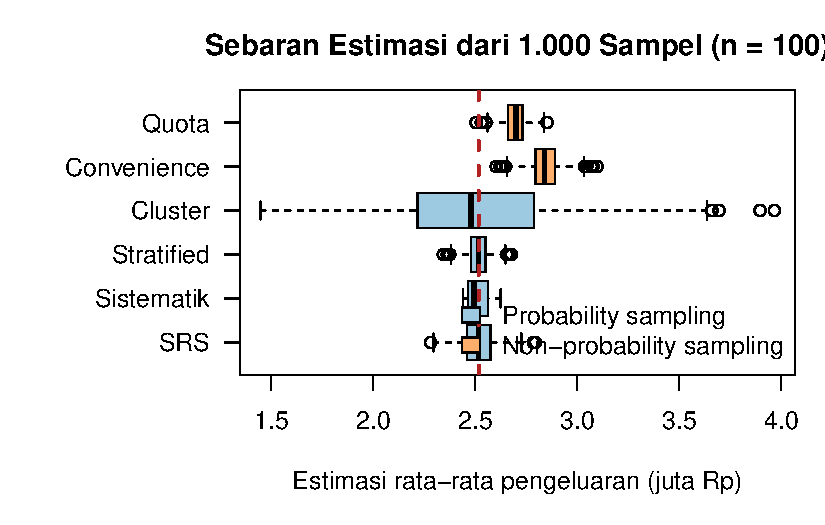
\includegraphics[keepaspectratio]{chapters/P03_files/figure-pdf/unnamed-chunk-24-1.pdf}}

\begin{Shaded}
\begin{Highlighting}[]
\FunctionTok{par}\NormalTok{(}\AttributeTok{mar =} \FunctionTok{c}\NormalTok{(}\DecValTok{5}\NormalTok{, }\DecValTok{4}\NormalTok{, }\DecValTok{4}\NormalTok{, }\DecValTok{2}\NormalTok{) }\SpecialCharTok{+} \FloatTok{0.1}\NormalTok{)}
\end{Highlighting}
\end{Shaded}

\textbf{Interpretasi:}

Keempat teknik probability sampling tidak bias -- kotaknya berpusat di
sekitar garis merah (parameter).

Stratified (dan sistematik pada kerangka yang terurut per fakultas)
paling presisi, karena variasi antarfakultas ``dikunci'' oleh desain.

Cluster paling tidak presisi: sampel dari 2 kelas bisa saja kebetulan
dua kelas Kedokteran (sangat boros) atau dua kelas Sains (hemat).

Convenience dan quota bias -- kotaknya bergeser ke kanan. Bias ini tidak
hilang meskipun diulang ribuan kali.

\subsection{Memperbesar Sampel Tidak Menyembuhkan
Bias}\label{memperbesar-sampel-tidak-menyembuhkan-bias}

\begin{Shaded}
\begin{Highlighting}[]
\FunctionTok{set.seed}\NormalTok{(}\DecValTok{2028}\NormalTok{)}
\NormalTok{srs\_kecil }\OtherTok{\textless{}{-}} \FunctionTok{replicate}\NormalTok{(}\DecValTok{500}\NormalTok{, }\FunctionTok{mean}\NormalTok{(pop}\SpecialCharTok{$}\NormalTok{pengeluaran[}\FunctionTok{sample}\NormalTok{(}\DecValTok{1}\SpecialCharTok{:}\NormalTok{N, }\DecValTok{50}\NormalTok{)]))}
\NormalTok{conv\_besar }\OtherTok{\textless{}{-}} \FunctionTok{replicate}\NormalTok{(}\DecValTok{500}\NormalTok{, }\FunctionTok{mean}\NormalTok{(pop}\SpecialCharTok{$}\NormalTok{pengeluaran[}\FunctionTok{sample}\NormalTok{(}\DecValTok{1}\SpecialCharTok{:}\NormalTok{N, }\DecValTok{800}\NormalTok{, }\AttributeTok{prob =}\NormalTok{ pop}\SpecialCharTok{$}\NormalTok{peluang\_kantin)]))}
\FunctionTok{par}\NormalTok{(}\AttributeTok{mar =} \FunctionTok{c}\NormalTok{(}\DecValTok{5}\NormalTok{, }\DecValTok{11}\NormalTok{, }\DecValTok{3}\NormalTok{, }\DecValTok{1}\NormalTok{))}
\FunctionTok{boxplot}\NormalTok{(}\FunctionTok{list}\NormalTok{(}\StringTok{"SRS, n = 50"} \OtherTok{=}\NormalTok{ srs\_kecil, }\StringTok{"Convenience, n = 800"} \OtherTok{=}\NormalTok{ conv\_besar), }\AttributeTok{horizontal =} \ConstantTok{TRUE}\NormalTok{, }\AttributeTok{las =} \DecValTok{1}\NormalTok{, }\AttributeTok{col =} \FunctionTok{c}\NormalTok{(}\StringTok{"\#9ecae1"}\NormalTok{, }\StringTok{"\#fdae6b"}\NormalTok{), }\AttributeTok{xlab =} \StringTok{"Estimasi rata{-}rata pengeluaran (juta Rp)"}\NormalTok{,}
\AttributeTok{main =} \StringTok{"Sampel Kecil yang Acak vs Sampel Besar yang Bias"}\NormalTok{)}
\FunctionTok{abline}\NormalTok{(}\AttributeTok{v =}\NormalTok{ mu\_pengeluaran, }\AttributeTok{col =} \StringTok{"firebrick"}\NormalTok{, }\AttributeTok{lwd =} \DecValTok{2}\NormalTok{, }\AttributeTok{lty =} \DecValTok{2}\NormalTok{)}
\end{Highlighting}
\end{Shaded}

\pandocbounded{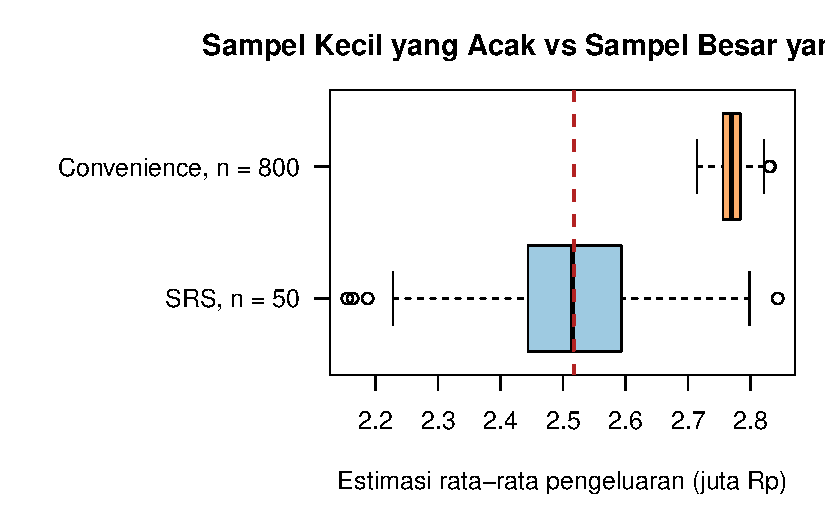
\includegraphics[keepaspectratio]{chapters/P03_files/figure-pdf/unnamed-chunk-26-1.pdf}}

\begin{Shaded}
\begin{Highlighting}[]
\FunctionTok{par}\NormalTok{(}\AttributeTok{mar =} \FunctionTok{c}\NormalTok{(}\DecValTok{5}\NormalTok{, }\DecValTok{4}\NormalTok{, }\DecValTok{4}\NormalTok{, }\DecValTok{2}\NormalTok{) }\SpecialCharTok{+} \FloatTok{0.1}\NormalTok{)}
\end{Highlighting}
\end{Shaded}

\emph{Convenience sample} berukuran 800 sangat \emph{presisi} (kotaknya
sempit) tetapi \textbf{presisi di tempat yang salah}. SRS berukuran 50
kurang presisi, tetapi berpusat di nilai yang benar. Memperbesar sampel
hanya mengecilkan \textbf{galat acak}, bukan \textbf{galat sistematik
(bias)}.

\section{Bias dalam Pengumpulan Data}\label{bias-dalam-pengumpulan-data}

\subsection{Akurasi vs Presisi}\label{akurasi-vs-presisi}

\textbf{Bias} adalah kesalahan \textbf{sistematik}: estimasi secara
konsisten melenceng ke satu arah. Berbeda dengan galat acak yang
``saling meniadakan'' bila diulang.

\begin{Shaded}
\begin{Highlighting}[]
\FunctionTok{set.seed}\NormalTok{(}\DecValTok{5}\NormalTok{)}
\NormalTok{papan\_target }\OtherTok{\textless{}{-}} \ControlFlowTok{function}\NormalTok{(pusat\_x, pusat\_y, sebaran, judul) \{}
\FunctionTok{plot}\NormalTok{(}\ConstantTok{NULL}\NormalTok{, }\AttributeTok{xlim =} \FunctionTok{c}\NormalTok{(}\SpecialCharTok{{-}}\DecValTok{3}\NormalTok{, }\DecValTok{3}\NormalTok{), }\AttributeTok{ylim =} \FunctionTok{c}\NormalTok{(}\SpecialCharTok{{-}}\DecValTok{3}\NormalTok{, }\DecValTok{3}\NormalTok{), }\AttributeTok{asp =} \DecValTok{1}\NormalTok{, }\AttributeTok{axes =} \ConstantTok{FALSE}\NormalTok{,}
\AttributeTok{xlab =} \StringTok{""}\NormalTok{, }\AttributeTok{ylab =} \StringTok{""}\NormalTok{, }\AttributeTok{main =}\NormalTok{ judul)}
\FunctionTok{symbols}\NormalTok{(}\FunctionTok{rep}\NormalTok{(}\DecValTok{0}\NormalTok{, }\DecValTok{3}\NormalTok{), }\FunctionTok{rep}\NormalTok{(}\DecValTok{0}\NormalTok{, }\DecValTok{3}\NormalTok{), }\AttributeTok{circles =} \FunctionTok{c}\NormalTok{(}\FloatTok{2.7}\NormalTok{, }\FloatTok{1.8}\NormalTok{, }\FloatTok{0.9}\NormalTok{), }\AttributeTok{inches =} \ConstantTok{FALSE}\NormalTok{,}
\AttributeTok{add =} \ConstantTok{TRUE}\NormalTok{, }\AttributeTok{fg =} \StringTok{"grey60"}\NormalTok{)}
\FunctionTok{points}\NormalTok{(}\DecValTok{0}\NormalTok{, }\DecValTok{0}\NormalTok{, }\AttributeTok{pch =} \DecValTok{3}\NormalTok{, }\AttributeTok{col =} \StringTok{"firebrick"}\NormalTok{, }\AttributeTok{cex =} \DecValTok{2}\NormalTok{, }\AttributeTok{lwd =} \DecValTok{2}\NormalTok{)}
\FunctionTok{points}\NormalTok{(}\FunctionTok{rnorm}\NormalTok{(}\DecValTok{25}\NormalTok{, pusat\_x, sebaran), }\FunctionTok{rnorm}\NormalTok{(}\DecValTok{25}\NormalTok{, pusat\_y, sebaran),}
\AttributeTok{pch =} \DecValTok{16}\NormalTok{, }\AttributeTok{col =} \FunctionTok{rgb}\NormalTok{(}\FloatTok{0.2}\NormalTok{, }\FloatTok{0.4}\NormalTok{, }\FloatTok{0.7}\NormalTok{, }\FloatTok{0.7}\NormalTok{))}
\NormalTok{\}}
\FunctionTok{par}\NormalTok{(}\AttributeTok{mfrow =} \FunctionTok{c}\NormalTok{(}\DecValTok{2}\NormalTok{, }\DecValTok{2}\NormalTok{), }\AttributeTok{mar =} \FunctionTok{c}\NormalTok{(}\DecValTok{1}\NormalTok{, }\DecValTok{1}\NormalTok{, }\DecValTok{3}\NormalTok{, }\DecValTok{1}\NormalTok{))}
\FunctionTok{papan\_target}\NormalTok{(}\DecValTok{0}\NormalTok{, }\DecValTok{0}\NormalTok{, }\FloatTok{0.3}\NormalTok{, }\StringTok{"Akurat \& Presisi}\SpecialCharTok{\textbackslash{}n}\StringTok{(tidak bias, sebaran kecil)"}\NormalTok{)}
\FunctionTok{papan\_target}\NormalTok{(}\DecValTok{0}\NormalTok{, }\DecValTok{0}\NormalTok{, }\FloatTok{1.0}\NormalTok{, }\StringTok{"Akurat, Tidak Presisi}\SpecialCharTok{\textbackslash{}n}\StringTok{(tidak bias, sebaran besar)"}\NormalTok{)}
\FunctionTok{papan\_target}\NormalTok{(}\FloatTok{1.4}\NormalTok{, }\FloatTok{1.2}\NormalTok{, }\FloatTok{0.3}\NormalTok{, }\StringTok{"Tidak Akurat, Presisi}\SpecialCharTok{\textbackslash{}n}\StringTok{(bias, sebaran kecil)"}\NormalTok{)}
\FunctionTok{papan\_target}\NormalTok{(}\FloatTok{1.2}\NormalTok{, }\FloatTok{1.0}\NormalTok{, }\FloatTok{1.0}\NormalTok{, }\StringTok{"Tidak Akurat \& Tidak Presisi"}\NormalTok{)}
\end{Highlighting}
\end{Shaded}

\pandocbounded{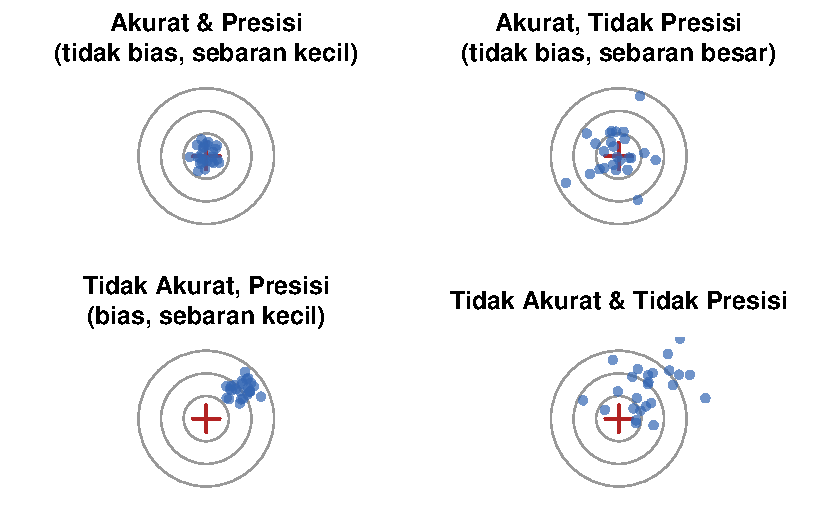
\includegraphics[keepaspectratio]{chapters/P03_files/figure-pdf/unnamed-chunk-28-1.pdf}}

\begin{Shaded}
\begin{Highlighting}[]
\FunctionTok{par}\NormalTok{(}\AttributeTok{mfrow =} \FunctionTok{c}\NormalTok{(}\DecValTok{1}\NormalTok{, }\DecValTok{1}\NormalTok{), }\AttributeTok{mar =} \FunctionTok{c}\NormalTok{(}\DecValTok{5}\NormalTok{, }\DecValTok{4}\NormalTok{, }\DecValTok{4}\NormalTok{, }\DecValTok{2}\NormalTok{) }\SpecialCharTok{+} \FloatTok{0.1}\NormalTok{)}
\end{Highlighting}
\end{Shaded}

Tanda silang merah adalah \textbf{parameter} yang ingin diduga;
titik-titik biru adalah estimasi dari sampel berulang.

\subsection{Jenis-jenis Bias}\label{jenis-jenis-bias}

{\def\LTcaptype{none} % do not increment counter
\begin{longtable}[]{@{}
  >{\raggedright\arraybackslash}p{(\linewidth - 6\tabcolsep) * \real{0.2500}}
  >{\raggedright\arraybackslash}p{(\linewidth - 6\tabcolsep) * \real{0.2500}}
  >{\raggedright\arraybackslash}p{(\linewidth - 6\tabcolsep) * \real{0.2500}}
  >{\raggedright\arraybackslash}p{(\linewidth - 6\tabcolsep) * \real{0.2500}}@{}}
\toprule\noalign{}
\begin{minipage}[b]{\linewidth}\raggedright
Jenis Bias
\end{minipage} & \begin{minipage}[b]{\linewidth}\raggedright
Terjadi pada tahap
\end{minipage} & \begin{minipage}[b]{\linewidth}\raggedright
Penyebab
\end{minipage} & \begin{minipage}[b]{\linewidth}\raggedright
Contoh
\end{minipage} \\
\midrule\noalign{}
\endhead
\bottomrule\noalign{}
\endlastfoot
\textbf{Sampling / selection bias} & Pemilihan sampel & Sebagian
populasi lebih (atau tidak) mungkin terpilih & \emph{Literary Digest};
survei di kantin \\
\textbf{\emph{Nonresponse bias}} & Pengumpulan & Yang \textbf{tidak
menjawab} berbeda secara sistematik dari yang menjawab & Mahasiswa yang
sibuk bekerja tidak sempat mengisi survei \\
\textbf{\emph{Response bias}} & Menjawab & Responden menjawab
\textbf{tidak jujur/tidak akurat} & Melebih-lebihkan jam belajar;
pertanyaan yang menggiring \\
\textbf{\emph{Measurement bias}} & Pengukuran & \textbf{Alat ukur} atau
prosedur keliru secara sistematik & Timbangan yang tidak dikalibrasi;
sensor TSS yang \emph{drift} \\
\end{longtable}
}

\subsubsection{Nonresponse Bias}\label{nonresponse-bias}

Survei dikirim ke 300 mahasiswa yang dipilih \textbf{acak} (desain sudah
benar). Namun mahasiswa yang banyak bekerja paruh waktu lebih jarang
membalas.

\begin{Shaded}
\begin{Highlighting}[]
\FunctionTok{set.seed}\NormalTok{(}\DecValTok{21}\NormalTok{)}
\NormalTok{diundang }\OtherTok{\textless{}{-}} \FunctionTok{sample}\NormalTok{(}\DecValTok{1}\SpecialCharTok{:}\NormalTok{N, }\DecValTok{300}\NormalTok{)}
\NormalTok{p\_membalas }\OtherTok{\textless{}{-}} \FunctionTok{plogis}\NormalTok{(}\FloatTok{1.2} \SpecialCharTok{{-}} \FloatTok{0.15} \SpecialCharTok{*}\NormalTok{ pop}\SpecialCharTok{$}\NormalTok{jam\_kerja[diundang]) }\CommentTok{\# makin sibuk, makin jarang membalas}
\NormalTok{membalas }\OtherTok{\textless{}{-}} \FunctionTok{rbinom}\NormalTok{(}\DecValTok{300}\NormalTok{, }\DecValTok{1}\NormalTok{, p\_membalas) }\SpecialCharTok{==} \DecValTok{1}
\FunctionTok{c}\NormalTok{(}\AttributeTok{Tingkat\_respons\_persen =} \FunctionTok{round}\NormalTok{(}\FunctionTok{mean}\NormalTok{(membalas) }\SpecialCharTok{*} \DecValTok{100}\NormalTok{, }\DecValTok{1}\NormalTok{),}
\AttributeTok{Rata\_jam\_kerja\_populasi =} \FunctionTok{round}\NormalTok{(}\FunctionTok{mean}\NormalTok{(pop}\SpecialCharTok{$}\NormalTok{jam\_kerja), }\DecValTok{2}\NormalTok{),}
\AttributeTok{Rata\_jam\_kerja\_diundang =} \FunctionTok{round}\NormalTok{(}\FunctionTok{mean}\NormalTok{(pop}\SpecialCharTok{$}\NormalTok{jam\_kerja[diundang]), }\DecValTok{2}\NormalTok{),}
\AttributeTok{Rata\_jam\_kerja\_responden =} \FunctionTok{round}\NormalTok{(}\FunctionTok{mean}\NormalTok{(pop}\SpecialCharTok{$}\NormalTok{jam\_kerja[diundang][membalas]), }\DecValTok{2}\NormalTok{))}
\end{Highlighting}
\end{Shaded}

\begin{verbatim}
  Tingkat_respons_persen  Rata_jam_kerja_populasi  Rata_jam_kerja_diundang 
                   52.30                     8.15                     7.76 
Rata_jam_kerja_responden 
                    5.46 
\end{verbatim}

Sampel yang \textbf{diundang} mewakili populasi, tetapi
\textbf{responden} yang membalas tidak -- rata-rata jam kerja paruh
waktu menjadi \textbf{terlalu rendah.} Pengacakan di awal tidak menolong
jika tingkat respons rendah dan terkait dengan variabel yang diukur.
Cara mengurangi: pengingat (follow-up), insentif, dan membandingkan
karakteristik responden dengan populasi.

\subsubsection{Response Bias}\label{response-bias}

Mahasiswa diminta \textbf{melaporkan sendiri} jam belajarnya. Karena
ingin terlihat rajin (social desirability), rata-rata mereka
melebih-lebihkan sekitar 3 jam.

\begin{Shaded}
\begin{Highlighting}[]
\FunctionTok{set.seed}\NormalTok{(}\DecValTok{22}\NormalTok{)}
\NormalTok{jam\_sebenarnya }\OtherTok{\textless{}{-}} \FunctionTok{round}\NormalTok{(}\FunctionTok{pmax}\NormalTok{(}\DecValTok{0}\NormalTok{, }\FunctionTok{rnorm}\NormalTok{(}\DecValTok{150}\NormalTok{, }\DecValTok{12}\NormalTok{, }\DecValTok{4}\NormalTok{)), }\DecValTok{1}\NormalTok{)}
\NormalTok{jam\_dilaporkan }\OtherTok{\textless{}{-}} \FunctionTok{round}\NormalTok{(jam\_sebenarnya }\SpecialCharTok{+} \FunctionTok{rnorm}\NormalTok{(}\DecValTok{150}\NormalTok{, }\AttributeTok{mean =} \DecValTok{3}\NormalTok{, }\AttributeTok{sd =} \FloatTok{1.5}\NormalTok{), }\DecValTok{1}\NormalTok{)}
\FunctionTok{c}\NormalTok{(}\AttributeTok{Rata\_sebenarnya =} \FunctionTok{mean}\NormalTok{(jam\_sebenarnya), }\AttributeTok{Rata\_dilaporkan =} \FunctionTok{mean}\NormalTok{(jam\_dilaporkan))}
\end{Highlighting}
\end{Shaded}

\begin{verbatim}
Rata_sebenarnya Rata_dilaporkan 
       11.79667        14.57733 
\end{verbatim}

\begin{Shaded}
\begin{Highlighting}[]
\FunctionTok{plot}\NormalTok{(jam\_sebenarnya, jam\_dilaporkan, }\AttributeTok{pch =} \DecValTok{16}\NormalTok{, }\AttributeTok{col =} \FunctionTok{rgb}\NormalTok{(}\FloatTok{0.2}\NormalTok{, }\FloatTok{0.4}\NormalTok{, }\FloatTok{0.7}\NormalTok{, }\FloatTok{0.6}\NormalTok{),}
\AttributeTok{xlab =} \StringTok{"Jam belajar sebenarnya (log aplikasi)"}\NormalTok{, }\AttributeTok{ylab =} \StringTok{"Jam belajar yang dilaporkan"}\NormalTok{,}
\AttributeTok{main =} \StringTok{"Response Bias: Hampir Semua Titik di Atas Garis y = x"}\NormalTok{)}
\FunctionTok{abline}\NormalTok{(}\DecValTok{0}\NormalTok{, }\DecValTok{1}\NormalTok{, }\AttributeTok{col =} \StringTok{"firebrick"}\NormalTok{, }\AttributeTok{lwd =} \DecValTok{2}\NormalTok{)}
\end{Highlighting}
\end{Shaded}

\pandocbounded{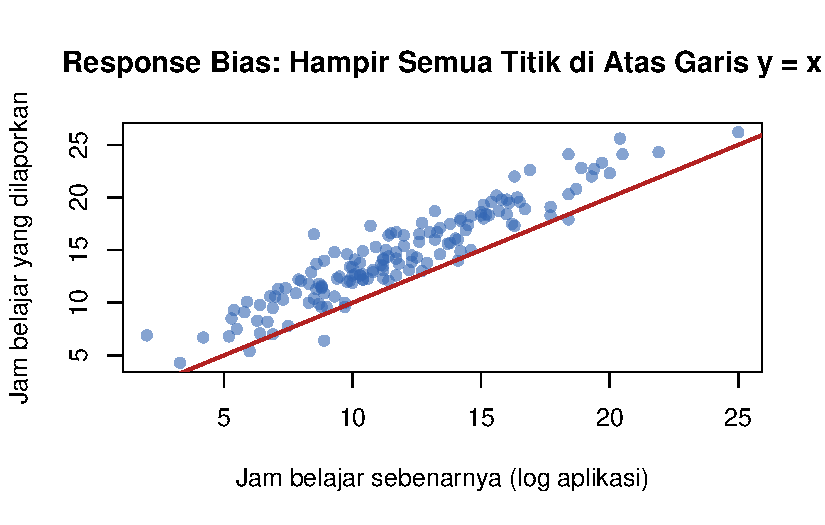
\includegraphics[keepaspectratio]{chapters/P03_files/figure-pdf/unnamed-chunk-32-1.pdf}}

\textbf{Bias susunan kalimat pertanyaan} juga termasuk \emph{response
bias:} \textbar{} Pertanyaan menggiring (hindari) \textbar{} Pertanyaan
netral (gunakan) \textbar{} \textbar{} :--- \textbar{} :--- \textbar{}
\textbar{} ``Setujukah Anda bahwa aplikasi baru yang \textbf{lebih
cepat} ini memudahkan Anda?'' \textbar{} ``Bagaimana penilaian Anda
terhadap kecepatan aplikasi baru?'' \textbar{} \textbar{} ``Berapa jam
Anda \textbf{membuang waktu} di media sosial setiap hari?'' \textbar{}
``Berapa jam rata-rata Anda menggunakan media sosial setiap hari?''
\textbar{} \textbar{} ``Apakah Anda puas dengan harga \textbf{dan}
pelayanan kami?'' (dua hal sekaligus) \textbar{} Pisahkan menjadi dua
pertanyaan: harga, lalu pelayanan \textbar{}

\subsubsection{Measurement Bias}\label{measurement-bias}

Dua sensor mengukur kadar TSS (mg/L) sampel air yang sama. Sensor B
belum dikalibrasi dan selalu membaca 8 mg/L lebih tinggi.

\begin{Shaded}
\begin{Highlighting}[]
\FunctionTok{set.seed}\NormalTok{(}\DecValTok{23}\NormalTok{)}
\NormalTok{tss\_sebenarnya }\OtherTok{\textless{}{-}} \DecValTok{48}
\NormalTok{sensor\_A }\OtherTok{\textless{}{-}} \FunctionTok{round}\NormalTok{(tss\_sebenarnya }\SpecialCharTok{+} \FunctionTok{rnorm}\NormalTok{(}\DecValTok{20}\NormalTok{, }\DecValTok{0}\NormalTok{, }\DecValTok{3}\NormalTok{), }\DecValTok{1}\NormalTok{) }\CommentTok{\# galat acak saja}
\NormalTok{sensor\_B }\OtherTok{\textless{}{-}} \FunctionTok{round}\NormalTok{(tss\_sebenarnya }\SpecialCharTok{+} \DecValTok{8} \SpecialCharTok{+} \FunctionTok{rnorm}\NormalTok{(}\DecValTok{20}\NormalTok{, }\DecValTok{0}\NormalTok{, }\DecValTok{1}\NormalTok{), }\DecValTok{1}\NormalTok{) }\CommentTok{\# bias +8, tetapi sangat konsisten}
\NormalTok{knitr}\SpecialCharTok{::}\FunctionTok{kable}\NormalTok{(}\FunctionTok{data.frame}\NormalTok{(}
\AttributeTok{Sensor =} \FunctionTok{c}\NormalTok{(}\StringTok{"A (terkalibrasi)"}\NormalTok{, }\StringTok{"B (tidak terkalibrasi)"}\NormalTok{),}
\AttributeTok{Rata\_pembacaan =} \FunctionTok{c}\NormalTok{(}\FunctionTok{mean}\NormalTok{(sensor\_A), }\FunctionTok{mean}\NormalTok{(sensor\_B)),}
\AttributeTok{SD\_pembacaan =} \FunctionTok{round}\NormalTok{(}\FunctionTok{c}\NormalTok{(}\FunctionTok{sd}\NormalTok{(sensor\_A), }\FunctionTok{sd}\NormalTok{(sensor\_B)), }\DecValTok{2}\NormalTok{),}
\AttributeTok{Bias =} \FunctionTok{round}\NormalTok{(}\FunctionTok{c}\NormalTok{(}\FunctionTok{mean}\NormalTok{(sensor\_A), }\FunctionTok{mean}\NormalTok{(sensor\_B)) }\SpecialCharTok{{-}}\NormalTok{ tss\_sebenarnya, }\DecValTok{2}\NormalTok{)}
\NormalTok{), }\AttributeTok{caption =} \StringTok{"Sensor B presisi tetapi tidak akurat"}\NormalTok{)}
\end{Highlighting}
\end{Shaded}

\begin{longtable}[]{@{}lrrr@{}}
\caption{Sensor B presisi tetapi tidak akurat}\tabularnewline
\toprule\noalign{}
Sensor & Rata\_pembacaan & SD\_pembacaan & Bias \\
\midrule\noalign{}
\endfirsthead
\toprule\noalign{}
Sensor & Rata\_pembacaan & SD\_pembacaan & Bias \\
\midrule\noalign{}
\endhead
\bottomrule\noalign{}
\endlastfoot
A (terkalibrasi) & 48.77 & 2.60 & 0.77 \\
B (tidak terkalibrasi) & 55.89 & 0.82 & 7.89 \\
\end{longtable}

Sensor B tampak ``lebih baik'' karena pembacaannya konsisten, padahal
selalu melenceng. Jika baku mutu TSS adalah 50 mg/L, sensor B akan
melaporkan \textbf{pelanggaran palsu} secara terus-menerus. Solusinya
adalah kalibrasi rutin terhadap standar.

\section{Studi Kasus Komprehensif: Merancang Survei Adopsi QRIS Pedagang
Pasar}\label{studi-kasus-komprehensif-merancang-survei-adopsi-qris-pedagang-pasar}

\textbf{Konteks}: Dinas Koperasi dan UMKM sebuah kabupaten ingin
mengetahui proporsi pedagang pasar tradisional yang sudah menerima
pembayaran QRIS. Terdapat daftar resmi \textbf{1.200 pedagang} di
\textbf{4 pasar}. Anggaran hanya cukup untuk mewawancarai \textbf{120
pedagang.} Diketahui pasar di pusat kota jauh lebih ``digital'' daripada
pasar di pinggiran.

\begin{Shaded}
\begin{Highlighting}[]
\FunctionTok{set.seed}\NormalTok{(}\DecValTok{404}\NormalTok{)}
\NormalTok{jml\_pasar }\OtherTok{\textless{}{-}} \FunctionTok{c}\NormalTok{(}\StringTok{"Pasar Sentral"} \OtherTok{=} \DecValTok{500}\NormalTok{, }\StringTok{"Pasar Baru"} \OtherTok{=} \DecValTok{350}\NormalTok{, }\StringTok{"Pasar Tani"} \OtherTok{=} \DecValTok{200}\NormalTok{,  }\StringTok{"Pasar Desa"} \OtherTok{=} \DecValTok{150}\NormalTok{)}
\NormalTok{adopsi\_psr }\OtherTok{\textless{}{-}} \FunctionTok{c}\NormalTok{(}\StringTok{"Pasar Sentral"} \OtherTok{=} \FloatTok{0.70}\NormalTok{, }\StringTok{"Pasar Baru"} \OtherTok{=} \FloatTok{0.55}\NormalTok{, }\StringTok{"Pasar Tani"} \OtherTok{=} \FloatTok{0.30}\NormalTok{, }\StringTok{"Pasar Desa"} \OtherTok{=} \FloatTok{0.15}\NormalTok{)}
\NormalTok{pedagang }\OtherTok{\textless{}{-}} \FunctionTok{data.frame}\NormalTok{(}\AttributeTok{id =} \FunctionTok{sprintf}\NormalTok{(}\StringTok{"PDG{-}\%04d"}\NormalTok{, }\DecValTok{1}\SpecialCharTok{:}\DecValTok{1200}\NormalTok{),}
\AttributeTok{pasar =} \FunctionTok{rep}\NormalTok{(}\FunctionTok{names}\NormalTok{(jml\_pasar), jml\_pasar))}
\NormalTok{pedagang}\SpecialCharTok{$}\NormalTok{qris }\OtherTok{\textless{}{-}} \FunctionTok{rbinom}\NormalTok{(}\DecValTok{1200}\NormalTok{, }\DecValTok{1}\NormalTok{, adopsi\_psr[pedagang}\SpecialCharTok{$}\NormalTok{pasar])}
\NormalTok{pedagang}\SpecialCharTok{$}\NormalTok{blok }\OtherTok{\textless{}{-}} \FunctionTok{paste}\NormalTok{(pedagang}\SpecialCharTok{$}\NormalTok{pasar, }\FunctionTok{ave}\NormalTok{(}\FunctionTok{seq\_len}\NormalTok{(}\DecValTok{1200}\NormalTok{), pedagang}\SpecialCharTok{$}\NormalTok{pasar,}
\AttributeTok{FUN =} \ControlFlowTok{function}\NormalTok{(i) }\FunctionTok{ceiling}\NormalTok{(}\FunctionTok{seq\_along}\NormalTok{(i) }\SpecialCharTok{/} \DecValTok{25}\NormalTok{)))}
\NormalTok{p\_populasi }\OtherTok{\textless{}{-}} \FunctionTok{mean}\NormalTok{(pedagang}\SpecialCharTok{$}\NormalTok{qris) }\CommentTok{\# dalam kenyataan tidak diketahui}
\FunctionTok{round}\NormalTok{(}\FunctionTok{tapply}\NormalTok{(pedagang}\SpecialCharTok{$}\NormalTok{qris, pedagang}\SpecialCharTok{$}\NormalTok{pasar, mean)[}\FunctionTok{names}\NormalTok{(jml\_pasar)], }\DecValTok{3}\NormalTok{)}
\end{Highlighting}
\end{Shaded}

\begin{verbatim}
Pasar Sentral    Pasar Baru    Pasar Tani    Pasar Desa 
        0.700         0.546         0.325         0.127 
\end{verbatim}

\subsection{Langkah 1: Menentukan Komponen
Survei}\label{langkah-1-menentukan-komponen-survei}

{\def\LTcaptype{none} % do not increment counter
\begin{longtable}[]{@{}
  >{\raggedright\arraybackslash}p{(\linewidth - 2\tabcolsep) * \real{0.5000}}
  >{\raggedright\arraybackslash}p{(\linewidth - 2\tabcolsep) * \real{0.5000}}@{}}
\toprule\noalign{}
\begin{minipage}[b]{\linewidth}\raggedright
Komponen
\end{minipage} & \begin{minipage}[b]{\linewidth}\raggedright
Keputusan
\end{minipage} \\
\midrule\noalign{}
\endhead
\bottomrule\noalign{}
\endlastfoot
Populasi & Seluruh pedagang pasar tradisional di kabupaten \\
Kerangka sampel & Daftar resmi 1.200 pedagang di 4 pasar (periksa:
apakah pedagang kaki lima tercatat?) \\
Unit observasi & Satu pedagang \\
Variabel utama & Menerima QRIS (Ya/Tidak) -- nominal biner \\
Metode pengumpulan & Wawancara terstruktur + \textbf{observasi}
keberadaan stiker/\emph{standee} QRIS di lapak \\
Teknik sampling & \textbf{\emph{Stratified}} menurut pasar, alokasi
proporsional (karena adopsi sangat berbeda antarpasar) \\
\end{longtable}
}

\subsection{Langkah 2: Alokasi dan Pengambilan
Sampel}\label{langkah-2-alokasi-dan-pengambilan-sampel}

\begin{Shaded}
\begin{Highlighting}[]
\NormalTok{n\_survei }\OtherTok{\textless{}{-}} \DecValTok{120}
\NormalTok{alok\_pasar }\OtherTok{\textless{}{-}} \FunctionTok{round}\NormalTok{(n\_survei }\SpecialCharTok{*}\NormalTok{ jml\_pasar }\SpecialCharTok{/} \FunctionTok{sum}\NormalTok{(jml\_pasar))}
\NormalTok{alok\_pasar}
\end{Highlighting}
\end{Shaded}

\begin{verbatim}
Pasar Sentral    Pasar Baru    Pasar Tani    Pasar Desa 
           50            35            20            15 
\end{verbatim}

\begin{Shaded}
\begin{Highlighting}[]
\FunctionTok{set.seed}\NormalTok{(}\DecValTok{405}\NormalTok{)}
\NormalTok{idx\_pasar }\OtherTok{\textless{}{-}} \FunctionTok{unlist}\NormalTok{(}\FunctionTok{lapply}\NormalTok{(}\FunctionTok{names}\NormalTok{(alok\_pasar), }\ControlFlowTok{function}\NormalTok{(p)}
\FunctionTok{sample}\NormalTok{(}\FunctionTok{which}\NormalTok{(pedagang}\SpecialCharTok{$}\NormalTok{pasar }\SpecialCharTok{==}\NormalTok{ p), alok\_pasar[[p]])))}
\NormalTok{sampel\_pasar }\OtherTok{\textless{}{-}}\NormalTok{ pedagang[idx\_pasar, ]}
\FunctionTok{head}\NormalTok{(sampel\_pasar[, }\FunctionTok{c}\NormalTok{(}\StringTok{"id"}\NormalTok{, }\StringTok{"pasar"}\NormalTok{)], }\DecValTok{8}\NormalTok{) }\CommentTok{\# daftar kerja untuk enumerator}
\end{Highlighting}
\end{Shaded}

\begin{verbatim}
          id         pasar
313 PDG-0313 Pasar Sentral
468 PDG-0468 Pasar Sentral
433 PDG-0433 Pasar Sentral
30  PDG-0030 Pasar Sentral
193 PDG-0193 Pasar Sentral
67  PDG-0067 Pasar Sentral
20  PDG-0020 Pasar Sentral
157 PDG-0157 Pasar Sentral
\end{verbatim}

\begin{Shaded}
\begin{Highlighting}[]
\NormalTok{p\_hat\_strata }\OtherTok{\textless{}{-}} \FunctionTok{mean}\NormalTok{(sampel\_pasar}\SpecialCharTok{$}\NormalTok{qris)}
\end{Highlighting}
\end{Shaded}

\subsection{Langkah 3: Membandingkan dengan Desain
Lain}\label{langkah-3-membandingkan-dengan-desain-lain}

\begin{Shaded}
\begin{Highlighting}[]
\FunctionTok{set.seed}\NormalTok{(}\DecValTok{406}\NormalTok{)}
\NormalTok{B }\OtherTok{\textless{}{-}} \DecValTok{1000}
\NormalTok{sim\_pasar }\OtherTok{\textless{}{-}} \FunctionTok{data.frame}\NormalTok{(}
\AttributeTok{Stratified =} \FunctionTok{replicate}\NormalTok{(B, \{}
\NormalTok{idx }\OtherTok{\textless{}{-}} \FunctionTok{unlist}\NormalTok{(}\FunctionTok{lapply}\NormalTok{(}\FunctionTok{names}\NormalTok{(alok\_pasar), }\ControlFlowTok{function}\NormalTok{(p)}
\FunctionTok{sample}\NormalTok{(}\FunctionTok{which}\NormalTok{(pedagang}\SpecialCharTok{$}\NormalTok{pasar }\SpecialCharTok{==}\NormalTok{ p), alok\_pasar[[p]])))}
\FunctionTok{mean}\NormalTok{(pedagang}\SpecialCharTok{$}\NormalTok{qris[idx])}
\NormalTok{\}),}
\AttributeTok{SRS =} \FunctionTok{replicate}\NormalTok{(B, }\FunctionTok{mean}\NormalTok{(pedagang}\SpecialCharTok{$}\NormalTok{qris[}\FunctionTok{sample}\NormalTok{(}\DecValTok{1}\SpecialCharTok{:}\DecValTok{1200}\NormalTok{, n\_survei)])), }\AttributeTok{Cluster\_blok =} \FunctionTok{replicate}\NormalTok{(B, \{}
\NormalTok{blok\_pilih }\OtherTok{\textless{}{-}} \FunctionTok{sample}\NormalTok{(}\FunctionTok{unique}\NormalTok{(pedagang}\SpecialCharTok{$}\NormalTok{blok), }\DecValTok{5}\NormalTok{) }\CommentTok{\# 5 blok x 25 lapak = 125 (mendekati 120)}
\FunctionTok{mean}\NormalTok{(pedagang}\SpecialCharTok{$}\NormalTok{qris[pedagang}\SpecialCharTok{$}\NormalTok{blok }\SpecialCharTok{\%in\%}\NormalTok{ blok\_pilih])}
\NormalTok{\}),}
\AttributeTok{Hanya\_Pasar\_Sentral =} \FunctionTok{replicate}\NormalTok{(B,  }\FunctionTok{mean}\NormalTok{(pedagang}\SpecialCharTok{$}\NormalTok{qris[}\FunctionTok{sample}\NormalTok{(}\FunctionTok{which}\NormalTok{(pedagang}\SpecialCharTok{$}\NormalTok{pasar }\SpecialCharTok{==}
\StringTok{"Pasar Sentral"}\NormalTok{), n\_survei)]))}
\NormalTok{)}
\NormalTok{knitr}\SpecialCharTok{::}\FunctionTok{kable}\NormalTok{(}\FunctionTok{data.frame}\NormalTok{(}
\AttributeTok{Desain =} \FunctionTok{names}\NormalTok{(sim\_pasar),}
\AttributeTok{Rata\_estimasi =} \FunctionTok{round}\NormalTok{(}\FunctionTok{colMeans}\NormalTok{(sim\_pasar), }\DecValTok{3}\NormalTok{),}
\AttributeTok{Bias =} \FunctionTok{round}\NormalTok{(}\FunctionTok{colMeans}\NormalTok{(sim\_pasar) }\SpecialCharTok{{-}}\NormalTok{ p\_populasi, }\DecValTok{3}\NormalTok{),}
\AttributeTok{SD\_estimasi =} \FunctionTok{round}\NormalTok{(}\FunctionTok{apply}\NormalTok{(sim\_pasar, }\DecValTok{2}\NormalTok{, sd), }\DecValTok{3}\NormalTok{),}
\AttributeTok{row.names =} \ConstantTok{NULL}
\NormalTok{), }\AttributeTok{caption =} \FunctionTok{paste0}\NormalTok{(}\StringTok{"Perbandingan desain survei (proporsi sebenarnya = "}\NormalTok{, }\FunctionTok{round}\NormalTok{(p\_populasi, }\DecValTok{3}\NormalTok{), }\StringTok{")"}\NormalTok{))}
\end{Highlighting}
\end{Shaded}

\begin{longtable}[]{@{}lrrr@{}}
\caption{Perbandingan desain survei (proporsi sebenarnya =
0.521)}\tabularnewline
\toprule\noalign{}
Desain & Rata\_estimasi & Bias & SD\_estimasi \\
\midrule\noalign{}
\endfirsthead
\toprule\noalign{}
Desain & Rata\_estimasi & Bias & SD\_estimasi \\
\midrule\noalign{}
\endhead
\bottomrule\noalign{}
\endlastfoot
Stratified & 0.519 & -0.002 & 0.040 \\
SRS & 0.522 & 0.001 & 0.044 \\
Cluster\_blok & 0.521 & 0.000 & 0.093 \\
Hanya\_Pasar\_Sentral & 0.699 & 0.178 & 0.036 \\
\end{longtable}

\subsection{Pertanyaan Diskusi dan
Jawaban}\label{pertanyaan-diskusi-dan-jawaban-2}

\textbf{1. Mengapa \emph{stratified sampling} menurut pasar adalah
pilihan terbaik?}

Karena tingkat adopsi QRIS \textbf{sangat berbeda antarpasar} (strata
homogen di dalam, berbeda antarstrata). Stratifikasi menjamin setiap
pasar terwakili sesuai proporsinya sehingga SD estimasinya paling kecil
di antara desain yang tidak bias. (Desain ``hanya Pasar Sentral'' memang
ber-SD kecil, tetapi presisi di nilai yang salah.) Hasil sampel kita: ̂𝑝
= 0.558 dibanding proporsi sebenarnya 0.521.

\textbf{2. Mengapa survei yang hanya dilakukan di Pasar Sentral
menyesatkan?}

Ini contoh \emph{purposive/convenience} sampling (pasar terbesar dan
termudah dijangkau). Estimasinya sekitar 0.7, jauh di atas proporsi
sebenarnya, karena Pasar Sentral adalah pasar paling digital. Kesimpulan
``mayoritas pedagang sudah memakai QRIS'' akan membuat pemerintah
\textbf{mengabaikan} pasar pinggiran yang paling membutuhkan
pendampingan.

\textbf{3. Kapan \emph{cluster} \emph{sampling} per blok layak dipilih?}

Jika biaya perjalanan antarlapak mahal atau kerangka per pedagang tidak
tersedia. Harganya adalah presisi lebih rendah (SD terbesar di antara
desain acak). Kompromi yang sering dipakai adalah \textbf{gabungan}:
stratifikasi per pasar, lalu memilih blok secara acak di dalam setiap
pasar (\emph{multistage sampling}).

\textbf{4. Bias apa yang masih mungkin muncul meskipun desainnya acak?}

\begin{enumerate}
\def\labelenumi{(\alph{enumi})}
\tightlist
\item
  \emph{Undercoverage}: pedagang tidak resmi tidak ada dalam daftar. (b)
  \emph{Nonresponse}: pedagang yang sibuk menolak diwawancarai. (c)
  \emph{Response bias}: pedagang mengaku ``menerima QRIS'' karena merasa
  diawasi dinas -- sebab itu wawancara dilengkapi \textbf{observasi}
  stiker QRIS di lapak
\end{enumerate}

\section{Latihan Mandiri}\label{latihan-mandiri-2}

\subsection{Latihan Utama: Survei Pengguna Transportasi
Umum}\label{latihan-utama-survei-pengguna-transportasi-umum}

\textbf{Konteks}: Pemerintah kota ingin memperkirakan rata-rata waktu
tempuh harian (menit) penglaju. Tersedia daftar 3.000 rumah tangga di 6
kecamatan (masing-masing dibagi menjadi RW berisi 50 rumah tangga).
Anggaran: 150 rumah tangga.

\begin{Shaded}
\begin{Highlighting}[]
\FunctionTok{set.seed}\NormalTok{(}\DecValTok{505}\NormalTok{)}
\NormalTok{kec }\OtherTok{\textless{}{-}} \FunctionTok{c}\NormalTok{(}\AttributeTok{Pusat =} \DecValTok{700}\NormalTok{, }\AttributeTok{Utara =} \DecValTok{600}\NormalTok{, }\AttributeTok{Selatan =} \DecValTok{550}\NormalTok{, }\AttributeTok{Timur =} \DecValTok{450}\NormalTok{, }\AttributeTok{Barat =} \DecValTok{400}\NormalTok{, }\AttributeTok{Pinggiran =} \DecValTok{300}\NormalTok{)}
\NormalTok{rata\_tempuh }\OtherTok{\textless{}{-}} \FunctionTok{c}\NormalTok{(}\AttributeTok{Pusat =} \DecValTok{35}\NormalTok{, }\AttributeTok{Utara =} \DecValTok{50}\NormalTok{, }\AttributeTok{Selatan =} \DecValTok{55}\NormalTok{, }\AttributeTok{Timur =} \DecValTok{60}\NormalTok{, }\AttributeTok{Barat =} \DecValTok{65}\NormalTok{, }\AttributeTok{Pinggiran =} \DecValTok{95}\NormalTok{)}
\NormalTok{rt }\OtherTok{\textless{}{-}} \FunctionTok{data.frame}\NormalTok{(}\AttributeTok{id =} \DecValTok{1}\SpecialCharTok{:}\DecValTok{3000}\NormalTok{, }\AttributeTok{kecamatan =} \FunctionTok{rep}\NormalTok{(}\FunctionTok{names}\NormalTok{(kec), kec))}
\NormalTok{rt}\SpecialCharTok{$}\NormalTok{rw }\OtherTok{\textless{}{-}} \FunctionTok{paste}\NormalTok{(rt}\SpecialCharTok{$}\NormalTok{kecamatan, }\FunctionTok{ave}\NormalTok{(rt}\SpecialCharTok{$}\NormalTok{id, rt}\SpecialCharTok{$}\NormalTok{kecamatan, }\AttributeTok{FUN =} \ControlFlowTok{function}\NormalTok{(i) }\FunctionTok{ceiling}\NormalTok{(}\FunctionTok{seq\_along}\NormalTok{(i) }\SpecialCharTok{/} \DecValTok{50}\NormalTok{)))}
\NormalTok{rt}\SpecialCharTok{$}\NormalTok{waktu\_tempuh }\OtherTok{\textless{}{-}} \FunctionTok{round}\NormalTok{(}\FunctionTok{pmax}\NormalTok{(}\DecValTok{5}\NormalTok{, }\FunctionTok{rnorm}\NormalTok{(}\DecValTok{3000}\NormalTok{, rata\_tempuh[rt}\SpecialCharTok{$}\NormalTok{kecamatan], }\DecValTok{12}\NormalTok{)))}
\NormalTok{mu\_tempuh }\OtherTok{\textless{}{-}} \FunctionTok{mean}\NormalTok{(rt}\SpecialCharTok{$}\NormalTok{waktu\_tempuh)}
\end{Highlighting}
\end{Shaded}

\subsubsection{Tugas 1: Ambil SRS berukuran 150 dan hitung rata-rata
waktu
tempuhnya}\label{tugas-1-ambil-srs-berukuran-150-dan-hitung-rata-rata-waktu-tempuhnya}

\begin{Shaded}
\begin{Highlighting}[]
\FunctionTok{set.seed}\NormalTok{(}\DecValTok{1}\NormalTok{)}
\FunctionTok{mean}\NormalTok{(rt}\SpecialCharTok{$}\NormalTok{waktu\_tempuh[}\FunctionTok{sample}\NormalTok{(}\DecValTok{1}\SpecialCharTok{:}\DecValTok{3000}\NormalTok{, }\DecValTok{150}\NormalTok{)])}
\end{Highlighting}
\end{Shaded}

\begin{verbatim}
[1] 54.4
\end{verbatim}

\subsubsection{\texorpdfstring{Tugas 2: Ambil \emph{systematic sample}
berukuran
150}{Tugas 2: Ambil systematic sample berukuran 150}}\label{tugas-2-ambil-systematic-sample-berukuran-150}

\begin{Shaded}
\begin{Highlighting}[]
\FunctionTok{set.seed}\NormalTok{(}\DecValTok{2}\NormalTok{)}
\NormalTok{k\_rt }\OtherTok{\textless{}{-}} \DecValTok{3000} \SpecialCharTok{/} \DecValTok{150}
\NormalTok{awal }\OtherTok{\textless{}{-}} \FunctionTok{sample}\NormalTok{(}\DecValTok{1}\SpecialCharTok{:}\NormalTok{k\_rt, }\DecValTok{1}\NormalTok{)}
\FunctionTok{mean}\NormalTok{(rt}\SpecialCharTok{$}\NormalTok{waktu\_tempuh[}\FunctionTok{seq}\NormalTok{(awal, }\AttributeTok{by =}\NormalTok{ k\_rt, }\AttributeTok{length.out =} \DecValTok{150}\NormalTok{)])}
\end{Highlighting}
\end{Shaded}

\begin{verbatim}
[1] 54.6
\end{verbatim}

\subsubsection{\texorpdfstring{Tugas 3: Ambil \emph{stratified sample}
proporsional menurut
kecamatan}{Tugas 3: Ambil stratified sample proporsional menurut kecamatan}}\label{tugas-3-ambil-stratified-sample-proporsional-menurut-kecamatan}

\begin{Shaded}
\begin{Highlighting}[]
\NormalTok{alok\_rt }\OtherTok{\textless{}{-}} \FunctionTok{round}\NormalTok{(}\DecValTok{150} \SpecialCharTok{*}\NormalTok{ kec }\SpecialCharTok{/} \FunctionTok{sum}\NormalTok{(kec))}
\NormalTok{alok\_rt}
\end{Highlighting}
\end{Shaded}

\begin{verbatim}
    Pusat     Utara   Selatan     Timur     Barat Pinggiran 
       35        30        28        22        20        15 
\end{verbatim}

\begin{Shaded}
\begin{Highlighting}[]
\FunctionTok{set.seed}\NormalTok{(}\DecValTok{3}\NormalTok{)}
\NormalTok{idx\_rt }\OtherTok{\textless{}{-}} \FunctionTok{unlist}\NormalTok{(}\FunctionTok{lapply}\NormalTok{(}\FunctionTok{names}\NormalTok{(alok\_rt), }\ControlFlowTok{function}\NormalTok{(kc)}
\FunctionTok{sample}\NormalTok{(}\FunctionTok{which}\NormalTok{(rt}\SpecialCharTok{$}\NormalTok{kecamatan }\SpecialCharTok{==}\NormalTok{ kc), alok\_rt[[kc]])))}
\FunctionTok{mean}\NormalTok{(rt}\SpecialCharTok{$}\NormalTok{waktu\_tempuh[idx\_rt])}
\end{Highlighting}
\end{Shaded}

\begin{verbatim}
[1] 55.78667
\end{verbatim}

\subsubsection{Tugas 4: Ambil cluster sample dengan memilih 3 RW secara
acak}\label{tugas-4-ambil-cluster-sample-dengan-memilih-3-rw-secara-acak}

\begin{Shaded}
\begin{Highlighting}[]
\FunctionTok{set.seed}\NormalTok{(}\DecValTok{4}\NormalTok{)}
\NormalTok{rw\_pilih }\OtherTok{\textless{}{-}} \FunctionTok{sample}\NormalTok{(}\FunctionTok{unique}\NormalTok{(rt}\SpecialCharTok{$}\NormalTok{rw), }\DecValTok{3}\NormalTok{)}
\NormalTok{rw\_pilih}
\end{Highlighting}
\end{Shaded}

\begin{verbatim}
[1] "Pinggiran 2" "Pusat 11"    "Barat 5"    
\end{verbatim}

\begin{Shaded}
\begin{Highlighting}[]
\FunctionTok{mean}\NormalTok{(rt}\SpecialCharTok{$}\NormalTok{waktu\_tempuh[rt}\SpecialCharTok{$}\NormalTok{rw }\SpecialCharTok{\%in\%}\NormalTok{ rw\_pilih])}
\end{Highlighting}
\end{Shaded}

\begin{verbatim}
[1] 65.53333
\end{verbatim}

\subsubsection{Tugas 5: Bandingkan keempat teknik dengan simulasi 500
ulangan}\label{tugas-5-bandingkan-keempat-teknik-dengan-simulasi-500-ulangan}

\begin{Shaded}
\begin{Highlighting}[]
\FunctionTok{set.seed}\NormalTok{(}\DecValTok{5}\NormalTok{)}
\NormalTok{sim\_rt }\OtherTok{\textless{}{-}} \FunctionTok{data.frame}\NormalTok{(}
\AttributeTok{SRS =} \FunctionTok{replicate}\NormalTok{(}\DecValTok{500}\NormalTok{, }\FunctionTok{mean}\NormalTok{(rt}\SpecialCharTok{$}\NormalTok{waktu\_tempuh[}\FunctionTok{sample}\NormalTok{(}\DecValTok{1}\SpecialCharTok{:}\DecValTok{3000}\NormalTok{, }\DecValTok{150}\NormalTok{)])),}
\AttributeTok{Sistematik =} \FunctionTok{replicate}\NormalTok{(}\DecValTok{500}\NormalTok{, \{}
\NormalTok{a }\OtherTok{\textless{}{-}} \FunctionTok{sample}\NormalTok{(}\DecValTok{1}\SpecialCharTok{:}\NormalTok{k\_rt, }\DecValTok{1}\NormalTok{); }\FunctionTok{mean}\NormalTok{(rt}\SpecialCharTok{$}\NormalTok{waktu\_tempuh[}\FunctionTok{seq}\NormalTok{(a, }\AttributeTok{by =}\NormalTok{ k\_rt, }\AttributeTok{length.out =} \DecValTok{150}\NormalTok{)])}
\NormalTok{\}),}
\AttributeTok{Stratified =} \FunctionTok{replicate}\NormalTok{(}\DecValTok{500}\NormalTok{, \{}
\NormalTok{idx }\OtherTok{\textless{}{-}} \FunctionTok{unlist}\NormalTok{(}\FunctionTok{lapply}\NormalTok{(}\FunctionTok{names}\NormalTok{(alok\_rt), }\ControlFlowTok{function}\NormalTok{(kc)}
\FunctionTok{sample}\NormalTok{(}\FunctionTok{which}\NormalTok{(rt}\SpecialCharTok{$}\NormalTok{kecamatan }\SpecialCharTok{==}\NormalTok{ kc), alok\_rt[[kc]])))}
\FunctionTok{mean}\NormalTok{(rt}\SpecialCharTok{$}\NormalTok{waktu\_tempuh[idx])}
\NormalTok{\}),}
\AttributeTok{Cluster =} \FunctionTok{replicate}\NormalTok{(}\DecValTok{500}\NormalTok{, }\FunctionTok{mean}\NormalTok{(rt}\SpecialCharTok{$}\NormalTok{waktu\_tempuh[rt}\SpecialCharTok{$}\NormalTok{rw }\SpecialCharTok{\%in\%} \FunctionTok{sample}\NormalTok{(}\FunctionTok{unique}\NormalTok{(rt}\SpecialCharTok{$}\NormalTok{rw), }\DecValTok{3}\NormalTok{)]))}
\NormalTok{)}
\FunctionTok{round}\NormalTok{(}\FunctionTok{rbind}\NormalTok{(}\AttributeTok{Bias =} \FunctionTok{colMeans}\NormalTok{(sim\_rt) }\SpecialCharTok{{-}}\NormalTok{ mu\_tempuh, }\AttributeTok{SD =} \FunctionTok{apply}\NormalTok{(sim\_rt, }\DecValTok{2}\NormalTok{, sd)), }\DecValTok{2}\NormalTok{)}
\end{Highlighting}
\end{Shaded}

\begin{verbatim}
      SRS Sistematik Stratified Cluster
Bias 0.03      -0.03       0.06    0.53
SD   1.59       1.23       0.96    9.93
\end{verbatim}

\begin{Shaded}
\begin{Highlighting}[]
\FunctionTok{boxplot}\NormalTok{(sim\_rt, }\AttributeTok{col =} \StringTok{"\#c7e9c0"}\NormalTok{, }\AttributeTok{ylab =} \StringTok{"Estimasi rata{-}rata waktu tempuh (menit)"}\NormalTok{,}
\AttributeTok{main =} \StringTok{"Perbandingan Teknik Sampling (500 ulangan)"}\NormalTok{)}
\FunctionTok{abline}\NormalTok{(}\AttributeTok{h =}\NormalTok{ mu\_tempuh, }\AttributeTok{col =} \StringTok{"firebrick"}\NormalTok{, }\AttributeTok{lwd =} \DecValTok{2}\NormalTok{, }\AttributeTok{lty =} \DecValTok{2}\NormalTok{)}
\end{Highlighting}
\end{Shaded}

\pandocbounded{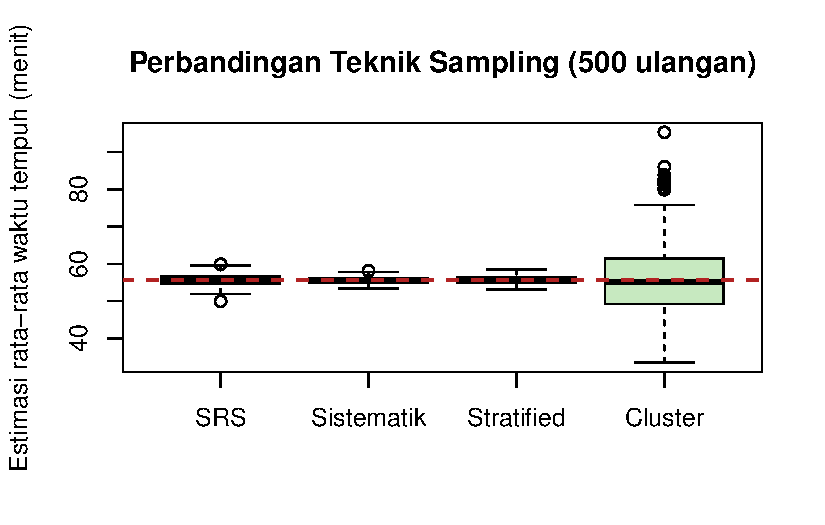
\includegraphics[keepaspectratio]{chapters/P03_files/figure-pdf/unnamed-chunk-47-1.pdf}}

\textbf{Jawaban}: Keempat teknik tidak bias (bias mendekati 0).
\emph{Stratified} dan sistematik (kerangka terurut per kecamatan)
memiliki SD terkecil karena waktu tempuh sangat berbeda antarkecamatan.
\emph{Cluster} 3 RW memiliki SD terbesar -- jika kebetulan terpilih RW
di Pinggiran, estimasinya melonjak.

\subsubsection{Tugas 6 (Tantangan): Bias survei di halte pusat
kota}\label{tugas-6-tantangan-bias-survei-di-halte-pusat-kota}

Petugas hanya mewawancarai penglaju di halte kecamatan Pusat.
Simulasikan estimasinya dan jelaskan arah biasnya.

\begin{Shaded}
\begin{Highlighting}[]
\FunctionTok{set.seed}\NormalTok{(}\DecValTok{6}\NormalTok{)}
\NormalTok{est\_halte }\OtherTok{\textless{}{-}} \FunctionTok{replicate}\NormalTok{(}\DecValTok{500}\NormalTok{, }\FunctionTok{mean}\NormalTok{(rt}\SpecialCharTok{$}\NormalTok{waktu\_tempuh[}\FunctionTok{sample}\NormalTok{(}\FunctionTok{which}\NormalTok{(rt}\SpecialCharTok{$}\NormalTok{kecamatan }\SpecialCharTok{==} \StringTok{"Pusat"}\NormalTok{), }\DecValTok{150}\NormalTok{)]))}
\FunctionTok{c}\NormalTok{(}\AttributeTok{Rata\_estimasi =} \FunctionTok{mean}\NormalTok{(est\_halte), }\AttributeTok{Parameter =}\NormalTok{ mu\_tempuh, }\AttributeTok{Bias =} \FunctionTok{mean}\NormalTok{(est\_halte) }\SpecialCharTok{{-}}\NormalTok{ mu\_tempuh)}
\end{Highlighting}
\end{Shaded}

\begin{verbatim}
Rata_estimasi     Parameter          Bias 
     35.22573      55.64200     -20.41627 
\end{verbatim}

\textbf{Jawaban}: Estimasi jauh \textbf{di bawah} parameter (bias
negatif) karena warga pusat kota tinggal dekat dengan tempat
aktivitasnya. Kebijakan yang didasarkan pada angka ini akan
\textbf{meremehkan} beban perjalanan warga pinggiran -- persis kelompok
yang paling membutuhkan layanan transportasi.

\subsection{Latihan Tambahan
(Self-Check)}\label{latihan-tambahan-self-check-2}

Kerjakan soal-soal berikut secara mandiri sebelum melihat kunci jawaban
pada komentar kode.

\textbf{Soal A.} Tentukan teknik sampling: (1) Memilih setiap pelanggan
ke-50 dari daftar CRM mulai dari nomor acak 17. (2) Membagi karyawan per
departemen lalu mengambil 10\% secara acak dari tiap departemen. (3)
Mengundi 5 sekolah dari 80 sekolah, lalu mensurvei semua guru di 5
sekolah itu. (4) Menyebar kuesioner melalui grup WhatsApp angkatan. (5)
Mewawancarai 8 kepala desa yang dianggap paling memahami konflik lahan.
(6) Mengisi 50 responden laki-laki dan 50 perempuan dari siapa pun yang
lewat di mal.

\begin{Shaded}
\begin{Highlighting}[]
\CommentTok{\# Kunci jawaban:}
\CommentTok{\# (1) Systematic (2) Stratified (proporsional) (3) Cluster}
\CommentTok{\# (4) Convenience (5) Purposive (6) Quota}
\end{Highlighting}
\end{Shaded}

\textbf{Soal B}. Sebuah aplikasi meminta pengguna memberi rating setelah
transaksi. Hanya 4\% pengguna yang memberi rating, dan rata-ratanya 4,8
dari 5. Bias apa yang paling mungkin? Mengapa?

\begin{Shaded}
\begin{Highlighting}[]
\CommentTok{\# Kunci jawaban:}
\CommentTok{\# Nonresponse bias (juga disebut voluntary response bias): pengguna yang memberi rating}
\CommentTok{\# sukarela cenderung yang sangat puas (atau sangat kecewa), tidak mewakili 96\% lainnya.}
\CommentTok{\# Rating 4,8 kemungkinan besar terlalu tinggi dibanding kepuasan seluruh pengguna.}
\end{Highlighting}
\end{Shaded}

\textbf{Soal C}. Dari populasi pop pada praktikum ini, ambil
\emph{stratified sample} berukuran 200 dengan alokasi proporsional
menurut fakultas, lalu bandingkan rata-rata pengeluarannya dengan
parameter.

\begin{Shaded}
\begin{Highlighting}[]
\CommentTok{\# Kunci jawaban:}
\NormalTok{alok200 }\OtherTok{\textless{}{-}} \FunctionTok{round}\NormalTok{(}\DecValTok{200} \SpecialCharTok{*}\NormalTok{ jumlah\_fak }\SpecialCharTok{/}\NormalTok{ N) }\CommentTok{\# 60, 50, 40, 30, 20}
\NormalTok{idx200 }\OtherTok{\textless{}{-}} \FunctionTok{unlist}\NormalTok{(}\FunctionTok{lapply}\NormalTok{(}\FunctionTok{names}\NormalTok{(alok200), }\ControlFlowTok{function}\NormalTok{(f)}
\FunctionTok{sample}\NormalTok{(}\FunctionTok{which}\NormalTok{(pop}\SpecialCharTok{$}\NormalTok{fakultas }\SpecialCharTok{==}\NormalTok{ f), alok200[[f]])))}
\FunctionTok{c}\NormalTok{(}\AttributeTok{Estimasi =} \FunctionTok{mean}\NormalTok{(pop}\SpecialCharTok{$}\NormalTok{pengeluaran[idx200]), }\AttributeTok{Parameter =}\NormalTok{ mu\_pengeluaran)}
\end{Highlighting}
\end{Shaded}

\begin{verbatim}
 Estimasi Parameter 
 2.573400  2.517125 
\end{verbatim}

\begin{Shaded}
\begin{Highlighting}[]
\CommentTok{\# Estimasi akan sangat dekat dengan parameter (selisih umumnya \textless{} 0,05 juta).}
\end{Highlighting}
\end{Shaded}

\textbf{Soal D}. Sebuah studi menemukan bahwa pengguna yang berlangganan
fitur premium berbelanja 40\% lebih banyak. Manajer menyimpulkan:
``Fitur premium membuat pengguna berbelanja lebih banyak.'' Kritik
kesimpulan ini dan usulkan desain yang lebih baik.

\begin{Shaded}
\begin{Highlighting}[]
\CommentTok{\# Kunci jawaban:}
\CommentTok{\# Studi ini observasional: pengguna MEMILIH SENDIRI berlangganan premium. Pengguna yang}
\CommentTok{\# memang sudah gemar berbelanja lebih mungkin berlangganan (confounding / self{-}selection).}
\CommentTok{\# Desain lebih baik: eksperimen (uji A/B) {-}{-} acak sebagian pengguna untuk menerima uji coba}
\CommentTok{\# premium gratis, lalu bandingkan belanja kelompok perlakuan dan kontrol.}
\end{Highlighting}
\end{Shaded}

\section{Kesalahan Umum dalam Pengumpulan dan Sampling
Data}\label{kesalahan-umum-dalam-pengumpulan-dan-sampling-data}

Mengira sampel besar pasti akurat -- sampel besar yang bias tetap bias
(Literary Digest).

Menyamakan ``acak'' dengan ``sembarangan'' -- memilih ``siapa saja yang
lewat'' adalah convenience sampling, bukan random sampling.

Tertukar antara stratified dan cluster -- stratified mengambil sebagian
unit dari setiap kelompok; cluster mengambil semua unit dari sebagian
kelompok.

Mengabaikan kualitas kerangka sampel -- unit yang tidak ada dalam daftar
tidak akan pernah terpilih.

Memakai systematic sampling pada daftar yang berpola periodik -- sampel
dapat selalu jatuh pada pola yang sama.

Menganggap quota sampling setara dengan stratified sampling --
komposisinya sama, tetapi pemilihan di dalam kuota tidak acak.

Mengabaikan tingkat respons -- sampel acak dengan tingkat respons rendah
dapat mengalami nonresponse bias.

Menyimpulkan sebab-akibat dari studi observasional -- gunakan eksperimen
dengan pengacakan bila memungkinkan.

Menulis pertanyaan yang menggiring atau bermakna ganda -- merusak data
sebelum dianalisis.

Menganggap alat ukur yang konsisten pasti benar -- presisi tidak sama
dengan akurasi; kalibrasi alat secara rutin.

Tidak mendokumentasikan metode sampling -- pembaca tidak dapat menilai
sejauh mana hasil dapat digeneralisasi.

\section{Cheat Sheet: Fungsi R yang
Digunakan}\label{cheat-sheet-fungsi-r-yang-digunakan-2}

{\def\LTcaptype{none} % do not increment counter
\begin{longtable}[]{@{}
  >{\raggedright\arraybackslash}p{(\linewidth - 2\tabcolsep) * \real{0.5000}}
  >{\raggedright\arraybackslash}p{(\linewidth - 2\tabcolsep) * \real{0.5000}}@{}}
\toprule\noalign{}
\begin{minipage}[b]{\linewidth}\raggedright
Fungsi
\end{minipage} & \begin{minipage}[b]{\linewidth}\raggedright
Kegunaan
\end{minipage} \\
\midrule\noalign{}
\endhead
\bottomrule\noalign{}
\endlastfoot
\texttt{sample(x,\ size)} & Simple random sampling tanpa pengembalian \\
\texttt{sample(x,\ size,\ prob\ =\ p)} & Pemilihan dengan peluang tidak
sama (simulasi bias/\emph{convenience}) \\
\texttt{sample(rep(c(0,\ 1),\ each\ =\ m))} & Pengacakan perlakuan dalam
eksperimen \\
\texttt{seq(from\ =\ r,\ by\ =\ k,\ length.out\ =\ n)} & Indeks
\emph{systematic sampling} \\
\texttt{which(kondisi)} & Indeks unit yang memenuhi kondisi (memilih
strata) \\
\texttt{lapply(daftar,\ fungsi)\ +\ unlist()} & Mengambil sampel dari
setiap strata lalu menggabungkannya \\
\texttt{x\ \%in\%\ daftar} & Memilih semua unit anggota klaster
terpilih \\
\texttt{unique(x)} & Daftar klaster/kategori unik \\
\texttt{round(n\ *\ N\_h\ /\ N)} & Alokasi proporsional \emph{stratified
sampling} \\
\texttt{replicate(B,\ ekspresi)} & Mengulang pengambilan sampel untuk
simulasi \\
\texttt{colMeans(df),\ apply(df,\ 2,\ sd)} & Rata-rata dan SD setiap
kolom hasil simulasi \\
\texttt{tapply(x,\ g,\ mean)} & Rata-rata per kelompok \\
\texttt{ave(x,\ g,\ FUN)} & Menghitung nilai per kelompok dengan panjang
tetap (membuat nomor klaster) \\
\texttt{rbinom(n,\ 1,\ p)} & Membangkitkan data biner Ya/Tidak \\
\texttt{plogis(z)} & Mengubah skor menjadi peluang 0--1 (untuk
simulasi) \\
\texttt{set.seed(k)} & Membuat hasil acak dapat direproduksi \\
\texttt{boxplot(list/df,\ horizontal\ =\ TRUE)} & Membandingkan sebaran
estimasi antarmetode \\
\texttt{symbols(...,\ circles\ =\ ...)} & Menggambar lingkaran (papan
target) \\
\end{longtable}
}

\section{Glosarium Istilah}\label{glosarium-istilah-2}

{\def\LTcaptype{none} % do not increment counter
\begin{longtable}[]{@{}
  >{\raggedright\arraybackslash}p{(\linewidth - 2\tabcolsep) * \real{0.5000}}
  >{\raggedright\arraybackslash}p{(\linewidth - 2\tabcolsep) * \real{0.5000}}@{}}
\toprule\noalign{}
\begin{minipage}[b]{\linewidth}\raggedright
Istilah
\end{minipage} & \begin{minipage}[b]{\linewidth}\raggedright
Definisi Singkat
\end{minipage} \\
\midrule\noalign{}
\endhead
\bottomrule\noalign{}
\endlastfoot
\textbf{Observasi} & Pengumpulan data dengan mencatat langsung tanpa
bertanya \\
\textbf{Survei} & Pengumpulan data dengan pertanyaan terstruktur kepada
banyak responden \\
\textbf{Wawancara} & Tanya jawab langsung antara peneliti dan
responden \\
\textbf{Eksperimen} & Studi di mana peneliti memberi perlakuan secara
acak lalu mengukur dampaknya \\
\textbf{Studi Observasional} & Studi tanpa pemberian perlakuan oleh
peneliti \\
\textbf{Random Assignment} & Pengacakan subjek ke kelompok
perlakuan/kontrol \\
\textbf{Variabel Pengganggu (Confounder)} & Variabel yang memengaruhi
perlakuan sekaligus hasil \\
\textbf{Kerangka Sampel} & Daftar unit populasi tempat sampel diambil \\
\textbf{Undercoverage} & Sebagian populasi tidak tercakup dalam kerangka
sampel \\
\textbf{Probability Sampling} & Pemilihan acak dengan peluang terpilih
yang diketahui \\
\textbf{Simple Random Sampling} & Setiap unit memiliki peluang terpilih
yang sama \\
\textbf{Systematic Sampling} & Memilih setiap unit ke-\emph{k} dari
titik awal acak \\
\textbf{Stratified Sampling} & SRS di dalam setiap strata (kelompok
homogen) \\
\textbf{Cluster Sampling} & Memilih klaster secara acak lalu mengamati
seluruh anggotanya \\
\textbf{Alokasi Proporsional} & Ukuran sampel tiap strata sebanding
ukuran strata di populasi \\
\textbf{Non-probability Sampling} & Pemilihan tidak acak; peluang
terpilih tidak diketahui \\
\textbf{Convenience / Purposive / Quota Sampling} & Memilih yang mudah
dijangkau / berdasarkan pertimbangan / memenuhi kuota \\
\textbf{Bias} & Kesalahan sistematik yang membuat estimasi melenceng ke
satu arah \\
\textbf{Akurasi / Presisi} & Kedekatan rata-rata estimasi dengan
parameter / kecilnya sebaran estimasi \\
\textbf{Sampling Bias} & Bias akibat cara pemilihan sampel \\
\textbf{Nonresponse Bias} & Bias karena yang tidak menjawab berbeda dari
yang menjawab \\
\textbf{Response Bias} & Bias karena jawaban responden tidak akurat atau
tidak jujur \\
\textbf{Measurement Bias} & Bias akibat alat atau prosedur pengukuran
yang keliru \\
\end{longtable}
}

\section{Rangkuman dan Kesimpulan}\label{rangkuman-dan-kesimpulan-2}

Cara data dikumpulkan menentukan kesimpulan yang boleh ditarik. Hanya
eksperimen dengan pengacakan yang kuat untuk menyimpulkan sebab-akibat;
studi observasional rentan confounding.{[}cite: 39{]}

Kerangka sampel harus mencakup populasi; undercoverage tidak dapat
diperbaiki oleh teknik sampling apa pun.{[}cite: 39{]}

Probability sampling (simple random, systematic, stratified, cluster)
menghasilkan estimasi tidak bias dan memungkinkan pengukuran
ketidakpastian. Stratified unggul dalam presisi; cluster unggul dalam
efisiensi biaya.{[}cite: 39{]}

Non-probability sampling berguna untuk eksplorasi, tetapi hasilnya tidak
dapat digeneralisasi secara sah.{[}cite: 39{]}

Bias adalah galat sistematik yang tidak hilang dengan memperbesar
sampel. Waspadai sampling bias, nonresponse bias, response bias, dan
measurement bias di setiap tahap.{[}cite: 39{]}

Akurasi dan presisi berbeda: alat atau sampel yang konsisten belum tentu
benar.{[}cite: 39{]}

\textbf{Jembatan ke sesi berikutnya}: setelah data terkumpul deng an
benar, Pertemuan 4 membahas cara \textbf{menyajikannya} -- tabel
frekuensi, frekuensi relatif dan kumulatif, serta visualisasi (diagram
batang, diagram lingkaran, histogram, \emph{stem-and-leaf}) beserta
prinsip visualisasi yang jujur.

\section{Referensi Pendukung}\label{referensi-pendukung-2}

Materi ini merangkum topik pengumpulan data dan teknik sampling
(\emph{data collection and sampling methods}) yang umum dibahas pada
buku teks pengantar statistika bisnis/data science. Mahasiswa disarankan
melengkapi pemahaman dengan merujuk pada:

Modul/slide perkuliahan ``Introduction to Statistics (SDT-1102)'' --
Pertemuan 3: Pengumpulan dan Sampling Data.

Squire, P. (1988). Why the 1936 Literary Digest Poll Failed. Public
Opinion Quarterly, 52(1), 125--133.

Lohr, S. L. Sampling: Design and Analysis. CRC Press (bab pendahuluan,
stratified, dan cluster sampling).

Dokumentasi resmi R: ?sample, ?seq, ?replicate, ?tapply, ?ave (dapat
diakses langsung di R/RStudio).

\bookmarksetup{startatroot}

\chapter{Penyajian dan Visualisasi
Data}\label{penyajian-dan-visualisasi-data}

\section{Data yang Dipakai}\label{data-yang-dipakai}

Tiga dataset dipakai sepanjang praktikum. Dataset nilai ujian dan
pendapatan mingguan akan \textbf{dipakai lagi} pada Pertemuan 5 (ukuran
pemusatan dan penyebaran), jadi pastikan Anda memahaminya.

\begin{Shaded}
\begin{Highlighting}[]
\CommentTok{\# 1. Kategorik: metode pembayaran 60 transaksi sebuah kedai kopi}
\FunctionTok{set.seed}\NormalTok{(}\DecValTok{404}\NormalTok{)}
\NormalTok{metode }\OtherTok{\textless{}{-}} \FunctionTok{sample}\NormalTok{(}\FunctionTok{c}\NormalTok{(}\StringTok{"QRIS"}\NormalTok{, }\StringTok{"Tunai"}\NormalTok{, }\StringTok{"Debit"}\NormalTok{, }\StringTok{"E{-}Wallet"}\NormalTok{, }\StringTok{"Kartu Kredit"}\NormalTok{), }\DecValTok{60}\NormalTok{, }\AttributeTok{replace =} \ConstantTok{TRUE}\NormalTok{,}
\AttributeTok{prob =} \FunctionTok{c}\NormalTok{(}\FloatTok{0.38}\NormalTok{, }\FloatTok{0.22}\NormalTok{, }\FloatTok{0.18}\NormalTok{, }\FloatTok{0.15}\NormalTok{, }\FloatTok{0.07}\NormalTok{))}
\NormalTok{waktu }\OtherTok{\textless{}{-}} \FunctionTok{sample}\NormalTok{(}\FunctionTok{c}\NormalTok{(}\StringTok{"Pagi"}\NormalTok{, }\StringTok{"Siang"}\NormalTok{, }\StringTok{"Malam"}\NormalTok{), }\DecValTok{60}\NormalTok{, }\AttributeTok{replace =} \ConstantTok{TRUE}\NormalTok{)}
\CommentTok{\# 2. Numerik: nilai ujian Statistika 30 mahasiswa}
\NormalTok{nilai\_ujian }\OtherTok{\textless{}{-}} \FunctionTok{c}\NormalTok{(}\DecValTok{78}\NormalTok{, }\DecValTok{65}\NormalTok{, }\DecValTok{82}\NormalTok{, }\DecValTok{90}\NormalTok{, }\DecValTok{74}\NormalTok{, }\DecValTok{68}\NormalTok{, }\DecValTok{95}\NormalTok{, }\DecValTok{88}\NormalTok{, }\DecValTok{72}\NormalTok{, }\DecValTok{80}\NormalTok{,}
\DecValTok{91}\NormalTok{, }\DecValTok{77}\NormalTok{, }\DecValTok{63}\NormalTok{, }\DecValTok{85}\NormalTok{, }\DecValTok{79}\NormalTok{, }\DecValTok{92}\NormalTok{, }\DecValTok{70}\NormalTok{, }\DecValTok{84}\NormalTok{, }\DecValTok{76}\NormalTok{, }\DecValTok{89}\NormalTok{,}
\DecValTok{81}\NormalTok{, }\DecValTok{67}\NormalTok{, }\DecValTok{93}\NormalTok{, }\DecValTok{75}\NormalTok{, }\DecValTok{86}\NormalTok{, }\DecValTok{71}\NormalTok{, }\DecValTok{94}\NormalTok{, }\DecValTok{83}\NormalTok{, }\DecValTok{69}\NormalTok{, }\DecValTok{87}\NormalTok{)}
\CommentTok{\# 3. Numerik terkelompok: pendapatan mingguan (USD) 100 karyawan}
\NormalTok{kelas\_p }\OtherTok{\textless{}{-}} \FunctionTok{c}\NormalTok{(}\StringTok{"801{-}1000"}\NormalTok{, }\StringTok{"1001{-}1200"}\NormalTok{, }\StringTok{"1201{-}1400"}\NormalTok{, }\StringTok{"1401{-}1600"}\NormalTok{, }\StringTok{"1601{-}1800"}\NormalTok{, }\StringTok{"1801{-}2000"}\NormalTok{)}
\NormalTok{f\_p }\OtherTok{\textless{}{-}} \FunctionTok{c}\NormalTok{(}\DecValTok{9}\NormalTok{, }\DecValTok{22}\NormalTok{, }\DecValTok{39}\NormalTok{, }\DecValTok{15}\NormalTok{, }\DecValTok{9}\NormalTok{, }\DecValTok{6}\NormalTok{)}
\end{Highlighting}
\end{Shaded}

\section{Tabel Frekuensi Data
Kategorik}\label{tabel-frekuensi-data-kategorik}

\subsection{Frekuensi, Frekuensi Relatif, dan
Persentase}\label{frekuensi-frekuensi-relatif-dan-persentase}

{\def\LTcaptype{none} % do not increment counter
\begin{longtable}[]{@{}lll@{}}
\toprule\noalign{}
Kolom & Rumus & Arti \\
\midrule\noalign{}
\endhead
\bottomrule\noalign{}
\endlastfoot
Frekuensi (\(f\)) & hitung & Banyaknya data pada kategori \\
Frekuensi relatif & \(\frac{f}{n}\) & Proporsi (0 sampai 1) \\
Persentase & \(\frac{f}{n} \times 100\%\) & Proporsi dalam persen \\
\end{longtable}
}

\begin{Shaded}
\begin{Highlighting}[]
\NormalTok{f\_metode }\OtherTok{\textless{}{-}} \FunctionTok{table}\NormalTok{(metode)}
\NormalTok{f\_metode }\OtherTok{\textless{}{-}} \FunctionTok{sort}\NormalTok{(f\_metode, }\AttributeTok{decreasing =} \ConstantTok{TRUE}\NormalTok{) }\CommentTok{\# urutkan dari yang terbanyak}
\NormalTok{tabel\_metode }\OtherTok{\textless{}{-}} \FunctionTok{data.frame}\NormalTok{(}
\AttributeTok{Metode =} \FunctionTok{names}\NormalTok{(f\_metode),}
\AttributeTok{f =} \FunctionTok{as.numeric}\NormalTok{(f\_metode),}
\AttributeTok{f\_relatif =} \FunctionTok{round}\NormalTok{(}\FunctionTok{as.numeric}\NormalTok{(}\FunctionTok{prop.table}\NormalTok{(f\_metode)), }\DecValTok{3}\NormalTok{),}
\AttributeTok{Persen =} \FunctionTok{round}\NormalTok{(}\FunctionTok{as.numeric}\NormalTok{(}\FunctionTok{prop.table}\NormalTok{(f\_metode)) }\SpecialCharTok{*} \DecValTok{100}\NormalTok{, }\DecValTok{1}\NormalTok{)}
\NormalTok{)}
\NormalTok{tabel\_metode }\OtherTok{\textless{}{-}} \FunctionTok{rbind}\NormalTok{(tabel\_metode,}
\FunctionTok{data.frame}\NormalTok{(}\AttributeTok{Metode =} \StringTok{"Total"}\NormalTok{, }\AttributeTok{f =} \FunctionTok{sum}\NormalTok{(tabel\_metode}\SpecialCharTok{$}\NormalTok{f),}
\AttributeTok{f\_relatif =} \DecValTok{1}\NormalTok{, }\AttributeTok{Persen =} \DecValTok{100}\NormalTok{))}
\NormalTok{knitr}\SpecialCharTok{::}\FunctionTok{kable}\NormalTok{(tabel\_metode, }\AttributeTok{caption =} \StringTok{"Distribusi Frekuensi Metode Pembayaran (n = 60)"}\NormalTok{)}
\end{Highlighting}
\end{Shaded}

\begin{longtable}[]{@{}lrrr@{}}
\caption{Distribusi Frekuensi Metode Pembayaran (n = 60)}\tabularnewline
\toprule\noalign{}
Metode & f & f\_relatif & Persen \\
\midrule\noalign{}
\endfirsthead
\toprule\noalign{}
Metode & f & f\_relatif & Persen \\
\midrule\noalign{}
\endhead
\bottomrule\noalign{}
\endlastfoot
QRIS & 21 & 0.35 & 35 \\
Tunai & 15 & 0.25 & 25 \\
Debit & 9 & 0.15 & 15 \\
E-Wallet & 9 & 0.15 & 15 \\
Kartu Kredit & 6 & 0.10 & 10 \\
Total & 60 & 1.00 & 100 \\
\end{longtable}

\textbf{Frekuensi kumulatif untuk data nominal?} Kumulatif hanya
bermakna jika kategori memiliki \textbf{urutan} (ordinal atau numerik).
Pada data nominal seperti metode pembayaran, kumulatif baru bermakna
setelah diurutkan dari terbanyak -- dan itu pun hanya untuk analisis
Pareto (lihat bagian visualisasi).

\subsection{Tabel Silang (Tabel
Kontingensi)}\label{tabel-silang-tabel-kontingensi}

Untuk melihat hubungan \textbf{dua} variabel kategorik, gunakan tabel
silang.

\begin{Shaded}
\begin{Highlighting}[]
\NormalTok{silang }\OtherTok{\textless{}{-}} \FunctionTok{table}\NormalTok{(}\AttributeTok{Waktu =} \FunctionTok{factor}\NormalTok{(waktu, }\AttributeTok{levels =} \FunctionTok{c}\NormalTok{(}\StringTok{"Pagi"}\NormalTok{, }\StringTok{"Siang"}\NormalTok{, }\StringTok{"Malam"}\NormalTok{)),}
\AttributeTok{Metode =} \FunctionTok{factor}\NormalTok{(metode, }\AttributeTok{levels =} \FunctionTok{names}\NormalTok{(f\_metode)))}
\FunctionTok{addmargins}\NormalTok{(silang)}
\end{Highlighting}
\end{Shaded}

\begin{verbatim}
       Metode
Waktu   QRIS Tunai Debit E-Wallet Kartu Kredit Sum
  Pagi     5     3     3        4            3  18
  Siang    8     6     3        4            2  23
  Malam    8     6     3        1            1  19
  Sum     21    15     9        9            6  60
\end{verbatim}

\begin{Shaded}
\begin{Highlighting}[]
\CommentTok{\# Persentase per baris: komposisi metode pembayaran di setiap waktu}
\FunctionTok{round}\NormalTok{(}\FunctionTok{prop.table}\NormalTok{(silang, }\AttributeTok{margin =} \DecValTok{1}\NormalTok{) }\SpecialCharTok{*} \DecValTok{100}\NormalTok{, }\DecValTok{1}\NormalTok{)}
\end{Highlighting}
\end{Shaded}

\begin{verbatim}
       Metode
Waktu   QRIS Tunai Debit E-Wallet Kartu Kredit
  Pagi  27.8  16.7  16.7     22.2         16.7
  Siang 34.8  26.1  13.0     17.4          8.7
  Malam 42.1  31.6  15.8      5.3          5.3
\end{verbatim}

Persentase \textbf{per baris} menjawab ``di waktu tertentu, metode apa
yang dominan?''; persentase \textbf{per kolom} (margin = 2) menjawab
``transaksi QRIS paling banyak terjadi pada waktu apa?''. Pilih arah
persentase sesuai pertanyaan.

\section{Tabel Frekuensi Data
Numerik}\label{tabel-frekuensi-data-numerik}

Data numerik dengan banyak nilai berbeda perlu dikelompokkan ke dalam
kelas (interval). Langkah-langkahnya:

{\def\LTcaptype{none} % do not increment counter
\begin{longtable}[]{@{}
  >{\raggedright\arraybackslash}p{(\linewidth - 4\tabcolsep) * \real{0.3333}}
  >{\raggedright\arraybackslash}p{(\linewidth - 4\tabcolsep) * \real{0.3333}}
  >{\raggedright\arraybackslash}p{(\linewidth - 4\tabcolsep) * \real{0.3333}}@{}}
\toprule\noalign{}
\begin{minipage}[b]{\linewidth}\raggedright
Langkah
\end{minipage} & \begin{minipage}[b]{\linewidth}\raggedright
Keterangan
\end{minipage} & \begin{minipage}[b]{\linewidth}\raggedright
Rumus
\end{minipage} \\
\midrule\noalign{}
\endhead
\bottomrule\noalign{}
\endlastfoot
1 & Hitung rentang & \(R = x_{\text{max}} - x_{\text{min}}\) \\
2 & Tentukan banyak kelas(Aturan Sturges) &
\(k = 1 + 3,322 \log_{10} n\)(dibulatkan) \\
3 & Tentukan lebar kelas & \(w = \frac{R}{k}\) (dibulatkan \textbf{ke
atas}) \\
4 & Tentukan batas kelas & Mulai dari \(x_{\text{min}}\) (atau sedikitdi
bawahnya) \\
5 & Tentukan batas nyata & Batas bawah \(-0,5\) satuan;batas atas
\(+0,5\) satuan \\
6 & Hitung titik tengah &
\(m = \frac{\text{batas bawah} + \text{batas atas}}{2}\) \\
7 & Hitung frekuensi tiap kelas & Turus / \texttt{cut()} +
\texttt{table()} \\
\end{longtable}
}

\subsection{Langkah demi Langkah: Nilai
Ujian}\label{langkah-demi-langkah-nilai-ujian}

\begin{Shaded}
\begin{Highlighting}[]
\NormalTok{n }\OtherTok{\textless{}{-}} \FunctionTok{length}\NormalTok{(nilai\_ujian)}
\NormalTok{R }\OtherTok{\textless{}{-}} \FunctionTok{max}\NormalTok{(nilai\_ujian) }\SpecialCharTok{{-}} \FunctionTok{min}\NormalTok{(nilai\_ujian)}
\NormalTok{k\_sturges }\OtherTok{\textless{}{-}} \DecValTok{1} \SpecialCharTok{+} \FloatTok{3.322} \SpecialCharTok{*} \FunctionTok{log10}\NormalTok{(n)}
\NormalTok{k }\OtherTok{\textless{}{-}} \FunctionTok{round}\NormalTok{(k\_sturges)}
\NormalTok{w }\OtherTok{\textless{}{-}} \FunctionTok{ceiling}\NormalTok{(R }\SpecialCharTok{/}\NormalTok{ k)}
\FunctionTok{c}\NormalTok{(}\AttributeTok{n =}\NormalTok{ n, }\AttributeTok{Min =} \FunctionTok{min}\NormalTok{(nilai\_ujian), }\AttributeTok{Maks =} \FunctionTok{max}\NormalTok{(nilai\_ujian), }\AttributeTok{Rentang =}\NormalTok{ R,}
\AttributeTok{k\_Sturges =} \FunctionTok{round}\NormalTok{(k\_sturges, }\DecValTok{3}\NormalTok{), }\AttributeTok{k =}\NormalTok{ k, }\AttributeTok{R\_per\_k =} \FunctionTok{round}\NormalTok{(R }\SpecialCharTok{/}\NormalTok{ k, }\DecValTok{3}\NormalTok{), }\AttributeTok{Lebar\_w =}\NormalTok{ w)}
\end{Highlighting}
\end{Shaded}

\begin{verbatim}
        n       Min      Maks   Rentang k_Sturges         k   R_per_k   Lebar_w 
   30.000    63.000    95.000    32.000     5.907     6.000     5.333     6.000 
\end{verbatim}

Diperoleh 𝑘 = 1+3,322 log10 30 ≈ 5.91 → 6 kelas, dan lebar kelas 𝑤 =
32/6 ≈ 5,33 → 6 (dibulatkan ke atas agar seluruh data tertampung).

\begin{Shaded}
\begin{Highlighting}[]
\NormalTok{batas\_bawah }\OtherTok{\textless{}{-}} \FunctionTok{seq}\NormalTok{(}\FunctionTok{min}\NormalTok{(nilai\_ujian), }\AttributeTok{by =}\NormalTok{ w, }\AttributeTok{length.out =}\NormalTok{ k) }\CommentTok{\# 63, 69, ..., 93}
\NormalTok{batas\_atas }\OtherTok{\textless{}{-}}\NormalTok{ batas\_bawah }\SpecialCharTok{+}\NormalTok{ w }\SpecialCharTok{{-}} \DecValTok{1} \CommentTok{\# 68, 74, ..., 98}
\NormalTok{batas\_nyata\_u }\OtherTok{\textless{}{-}} \FunctionTok{c}\NormalTok{(batas\_bawah }\SpecialCharTok{{-}} \FloatTok{0.5}\NormalTok{, }\FunctionTok{max}\NormalTok{(batas\_atas) }\SpecialCharTok{+} \FloatTok{0.5}\NormalTok{) }\CommentTok{\# 62.5, 68.5, ..., 98.5}
\NormalTok{f\_ujian }\OtherTok{\textless{}{-}} \FunctionTok{as.numeric}\NormalTok{(}\FunctionTok{table}\NormalTok{(}\FunctionTok{cut}\NormalTok{(nilai\_ujian, }\AttributeTok{breaks =}\NormalTok{ batas\_nyata\_u)))}
\NormalTok{tabel\_ujian }\OtherTok{\textless{}{-}} \FunctionTok{data.frame}\NormalTok{(}
\AttributeTok{Kelas =} \FunctionTok{paste0}\NormalTok{(batas\_bawah, }\StringTok{"{-}"}\NormalTok{, batas\_atas),}
\AttributeTok{Batas\_Nyata =} \FunctionTok{paste0}\NormalTok{(batas\_bawah }\SpecialCharTok{{-}} \FloatTok{0.5}\NormalTok{, }\StringTok{"{-}"}\NormalTok{, batas\_atas }\SpecialCharTok{+} \FloatTok{0.5}\NormalTok{),}
\AttributeTok{Titik\_Tengah =}\NormalTok{ (batas\_bawah }\SpecialCharTok{+}\NormalTok{ batas\_atas) }\SpecialCharTok{/} \DecValTok{2}\NormalTok{,}
\AttributeTok{f =}\NormalTok{ f\_ujian,}
\AttributeTok{f\_Relatif =} \FunctionTok{round}\NormalTok{(f\_ujian }\SpecialCharTok{/}\NormalTok{ n, }\DecValTok{3}\NormalTok{),}
\AttributeTok{Persen =} \FunctionTok{round}\NormalTok{(f\_ujian }\SpecialCharTok{/}\NormalTok{ n }\SpecialCharTok{*} \DecValTok{100}\NormalTok{, }\DecValTok{1}\NormalTok{),}
\AttributeTok{F\_Kumulatif =} \FunctionTok{cumsum}\NormalTok{(f\_ujian),}
\AttributeTok{Persen\_Kum =} \FunctionTok{round}\NormalTok{(}\FunctionTok{cumsum}\NormalTok{(f\_ujian) }\SpecialCharTok{/}\NormalTok{ n }\SpecialCharTok{*} \DecValTok{100}\NormalTok{, }\DecValTok{1}\NormalTok{)}
\NormalTok{)}
\NormalTok{knitr}\SpecialCharTok{::}\FunctionTok{kable}\NormalTok{(tabel\_ujian, }\AttributeTok{caption =} \StringTok{"Distribusi Frekuensi Nilai Ujian Statistika (n = 30)"}\NormalTok{)}
\end{Highlighting}
\end{Shaded}

\begin{longtable}[]{@{}
  >{\raggedright\arraybackslash}p{(\linewidth - 14\tabcolsep) * \real{0.0811}}
  >{\raggedright\arraybackslash}p{(\linewidth - 14\tabcolsep) * \real{0.1622}}
  >{\raggedleft\arraybackslash}p{(\linewidth - 14\tabcolsep) * \real{0.1757}}
  >{\raggedleft\arraybackslash}p{(\linewidth - 14\tabcolsep) * \real{0.0405}}
  >{\raggedleft\arraybackslash}p{(\linewidth - 14\tabcolsep) * \real{0.1351}}
  >{\raggedleft\arraybackslash}p{(\linewidth - 14\tabcolsep) * \real{0.0946}}
  >{\raggedleft\arraybackslash}p{(\linewidth - 14\tabcolsep) * \real{0.1622}}
  >{\raggedleft\arraybackslash}p{(\linewidth - 14\tabcolsep) * \real{0.1486}}@{}}
\caption{Distribusi Frekuensi Nilai Ujian Statistika (n =
30)}\tabularnewline
\toprule\noalign{}
\begin{minipage}[b]{\linewidth}\raggedright
Kelas
\end{minipage} & \begin{minipage}[b]{\linewidth}\raggedright
Batas\_Nyata
\end{minipage} & \begin{minipage}[b]{\linewidth}\raggedleft
Titik\_Tengah
\end{minipage} & \begin{minipage}[b]{\linewidth}\raggedleft
f
\end{minipage} & \begin{minipage}[b]{\linewidth}\raggedleft
f\_Relatif
\end{minipage} & \begin{minipage}[b]{\linewidth}\raggedleft
Persen
\end{minipage} & \begin{minipage}[b]{\linewidth}\raggedleft
F\_Kumulatif
\end{minipage} & \begin{minipage}[b]{\linewidth}\raggedleft
Persen\_Kum
\end{minipage} \\
\midrule\noalign{}
\endfirsthead
\toprule\noalign{}
\begin{minipage}[b]{\linewidth}\raggedright
Kelas
\end{minipage} & \begin{minipage}[b]{\linewidth}\raggedright
Batas\_Nyata
\end{minipage} & \begin{minipage}[b]{\linewidth}\raggedleft
Titik\_Tengah
\end{minipage} & \begin{minipage}[b]{\linewidth}\raggedleft
f
\end{minipage} & \begin{minipage}[b]{\linewidth}\raggedleft
f\_Relatif
\end{minipage} & \begin{minipage}[b]{\linewidth}\raggedleft
Persen
\end{minipage} & \begin{minipage}[b]{\linewidth}\raggedleft
F\_Kumulatif
\end{minipage} & \begin{minipage}[b]{\linewidth}\raggedleft
Persen\_Kum
\end{minipage} \\
\midrule\noalign{}
\endhead
\bottomrule\noalign{}
\endlastfoot
63-68 & 62.5-68.5 & 65.5 & 4 & 0.133 & 13.3 & 4 & 13.3 \\
69-74 & 68.5-74.5 & 71.5 & 5 & 0.167 & 16.7 & 9 & 30.0 \\
75-80 & 74.5-80.5 & 77.5 & 6 & 0.200 & 20.0 & 15 & 50.0 \\
81-86 & 80.5-86.5 & 83.5 & 6 & 0.200 & 20.0 & 21 & 70.0 \\
87-92 & 86.5-92.5 & 89.5 & 6 & 0.200 & 20.0 & 27 & 90.0 \\
93-98 & 92.5-98.5 & 95.5 & 3 & 0.100 & 10.0 & 30 & 100.0 \\
\end{longtable}

\textbf{Mengapa batas nyata?} Nilai ujian dicatat sebagai bilangan
bulat. Batas nyata (±0,5) menutup ``celah'' antara kelas 63--68 dan
69--74 sehingga setiap kemungkinan nilai (misalnya 68,7 bila dibulatkan)
punya tempat yang jelas, dan batang histogram saling menempel tanpa
celah.

\textbf{Cara membaca:}

\begin{itemize}
\tightlist
\item
  Kelas dengan frekuensi terbanyak adalah kelas 75-80, 81-86, 87-92
  (masing-masing 6 mahasiswa).
\item
  50\% mahasiswa bernilai 80 atau kurang (frekuensi kumulatif relatif
  kelas ketiga).
\item
  Hanya 3 mahasiswa (10\%) berada di kelas tertinggi 93--98.
\end{itemize}

\textbf{Konvensi interval di R.} \texttt{cut()} secara bawaan memakai
interval tertutup kanan \texttt{(a,\ b{]}}. Karena batas nyata berakhir
di ,5 dan data berupa bilangan bulat, tidak ada data yang jatuh tepat di
batas, sehingga konvensi ini tidak menjadi masalah.

\subsection{\texorpdfstring{Kelas Lebar Sama dengan
\texttt{hist()}}{Kelas Lebar Sama dengan hist()}}\label{kelas-lebar-sama-dengan-hist}

Fungsi \texttt{hist()} juga menghitung frekuensi kelas jika diberi
argumen \texttt{plot\ =\ FALSE}:

\begin{Shaded}
\begin{Highlighting}[]
\NormalTok{h }\OtherTok{\textless{}{-}} \FunctionTok{hist}\NormalTok{(nilai\_ujian, }\AttributeTok{breaks =}\NormalTok{ batas\_nyata\_u, }\AttributeTok{plot =} \ConstantTok{FALSE}\NormalTok{)}
\FunctionTok{data.frame}\NormalTok{(}\AttributeTok{dari =} \FunctionTok{head}\NormalTok{(h}\SpecialCharTok{$}\NormalTok{breaks, }\SpecialCharTok{{-}}\DecValTok{1}\NormalTok{), }\AttributeTok{sampai =} \FunctionTok{tail}\NormalTok{(h}\SpecialCharTok{$}\NormalTok{breaks, }\SpecialCharTok{{-}}\DecValTok{1}\NormalTok{),}
\AttributeTok{titik\_tengah =}\NormalTok{ h}\SpecialCharTok{$}\NormalTok{mids, }\AttributeTok{f =}\NormalTok{ h}\SpecialCharTok{$}\NormalTok{counts)}
\end{Highlighting}
\end{Shaded}

\begin{verbatim}
  dari sampai titik_tengah f
1 62.5   68.5         65.5 4
2 68.5   74.5         71.5 5
3 74.5   80.5         77.5 6
4 80.5   86.5         83.5 6
5 86.5   92.5         89.5 6
6 92.5   98.5         95.5 3
\end{verbatim}

\subsection{Data yang Sudah Terkelompok: Pendapatan
Mingguan}\label{data-yang-sudah-terkelompok-pendapatan-mingguan}

Sering kali kita hanya menerima tabel jadi tanpa data mentah. Kita tetap
dapat melengkapinya dengan kolom relatif dan kumulatif.

\begin{Shaded}
\begin{Highlighting}[]
\NormalTok{batas\_nyata\_p }\OtherTok{\textless{}{-}} \FunctionTok{seq}\NormalTok{(}\FloatTok{800.5}\NormalTok{, }\AttributeTok{by =} \DecValTok{200}\NormalTok{, }\AttributeTok{length.out =} \DecValTok{7}\NormalTok{)}
\NormalTok{L\_p }\OtherTok{\textless{}{-}} \FunctionTok{head}\NormalTok{(batas\_nyata\_p, }\SpecialCharTok{{-}}\DecValTok{1}\NormalTok{); U\_p }\OtherTok{\textless{}{-}} \FunctionTok{tail}\NormalTok{(batas\_nyata\_p, }\SpecialCharTok{{-}}\DecValTok{1}\NormalTok{)}
\NormalTok{n\_p }\OtherTok{\textless{}{-}} \FunctionTok{sum}\NormalTok{(f\_p)}
\NormalTok{tabel\_p }\OtherTok{\textless{}{-}} \FunctionTok{data.frame}\NormalTok{(}
\AttributeTok{Kelas =}\NormalTok{ kelas\_p,}
\AttributeTok{Batas\_Nyata =} \FunctionTok{paste0}\NormalTok{(L\_p, }\StringTok{"{-}"}\NormalTok{, U\_p),}
\AttributeTok{Titik\_Tengah =}\NormalTok{ (L\_p }\SpecialCharTok{+}\NormalTok{ U\_p) }\SpecialCharTok{/} \DecValTok{2}\NormalTok{,}
\AttributeTok{f =}\NormalTok{ f\_p,}
\AttributeTok{Persen =}\NormalTok{ f\_p }\SpecialCharTok{/}\NormalTok{ n\_p }\SpecialCharTok{*} \DecValTok{100}\NormalTok{,}
\AttributeTok{F\_Kum\_Kurang =} \FunctionTok{cumsum}\NormalTok{(f\_p), }\CommentTok{\# "kurang dari" batas nyata atas}
\AttributeTok{F\_Kum\_Lebih =} \FunctionTok{rev}\NormalTok{(}\FunctionTok{cumsum}\NormalTok{(}\FunctionTok{rev}\NormalTok{(f\_p))) }\CommentTok{\# "lebih dari" batas nyata bawah}
\NormalTok{)}
\NormalTok{knitr}\SpecialCharTok{::}\FunctionTok{kable}\NormalTok{(tabel\_p, }\AttributeTok{caption =} \StringTok{"Pendapatan Mingguan 100 Karyawan (USD)"}\NormalTok{)}
\end{Highlighting}
\end{Shaded}

\begin{longtable}[]{@{}
  >{\raggedright\arraybackslash}p{(\linewidth - 12\tabcolsep) * \real{0.1389}}
  >{\raggedright\arraybackslash}p{(\linewidth - 12\tabcolsep) * \real{0.1944}}
  >{\raggedleft\arraybackslash}p{(\linewidth - 12\tabcolsep) * \real{0.1806}}
  >{\raggedleft\arraybackslash}p{(\linewidth - 12\tabcolsep) * \real{0.0417}}
  >{\raggedleft\arraybackslash}p{(\linewidth - 12\tabcolsep) * \real{0.0972}}
  >{\raggedleft\arraybackslash}p{(\linewidth - 12\tabcolsep) * \real{0.1806}}
  >{\raggedleft\arraybackslash}p{(\linewidth - 12\tabcolsep) * \real{0.1667}}@{}}
\caption{Pendapatan Mingguan 100 Karyawan (USD)}\tabularnewline
\toprule\noalign{}
\begin{minipage}[b]{\linewidth}\raggedright
Kelas
\end{minipage} & \begin{minipage}[b]{\linewidth}\raggedright
Batas\_Nyata
\end{minipage} & \begin{minipage}[b]{\linewidth}\raggedleft
Titik\_Tengah
\end{minipage} & \begin{minipage}[b]{\linewidth}\raggedleft
f
\end{minipage} & \begin{minipage}[b]{\linewidth}\raggedleft
Persen
\end{minipage} & \begin{minipage}[b]{\linewidth}\raggedleft
F\_Kum\_Kurang
\end{minipage} & \begin{minipage}[b]{\linewidth}\raggedleft
F\_Kum\_Lebih
\end{minipage} \\
\midrule\noalign{}
\endfirsthead
\toprule\noalign{}
\begin{minipage}[b]{\linewidth}\raggedright
Kelas
\end{minipage} & \begin{minipage}[b]{\linewidth}\raggedright
Batas\_Nyata
\end{minipage} & \begin{minipage}[b]{\linewidth}\raggedleft
Titik\_Tengah
\end{minipage} & \begin{minipage}[b]{\linewidth}\raggedleft
f
\end{minipage} & \begin{minipage}[b]{\linewidth}\raggedleft
Persen
\end{minipage} & \begin{minipage}[b]{\linewidth}\raggedleft
F\_Kum\_Kurang
\end{minipage} & \begin{minipage}[b]{\linewidth}\raggedleft
F\_Kum\_Lebih
\end{minipage} \\
\midrule\noalign{}
\endhead
\bottomrule\noalign{}
\endlastfoot
801-1000 & 800.5-1000.5 & 900.5 & 9 & 9 & 9 & 100 \\
1001-1200 & 1000.5-1200.5 & 1100.5 & 22 & 22 & 31 & 91 \\
1201-1400 & 1200.5-1400.5 & 1300.5 & 39 & 39 & 70 & 69 \\
1401-1600 & 1400.5-1600.5 & 1500.5 & 15 & 15 & 85 & 30 \\
1601-1800 & 1600.5-1800.5 & 1700.5 & 9 & 9 & 94 & 15 \\
1801-2000 & 1800.5-2000.5 & 1900.5 & 6 & 6 & 100 & 6 \\
\end{longtable}

Kumulatif ``kurang dari'' menjawab: ``berapa karyawan berpendapatan di
bawah 1.400,5 USD?'' (70 orang). Kumulatif ``lebih dari'' menjawab:
``berapa karyawan berpendapatan di atas 1.400,5 USD?'' (30 orang).

\section{Visualisasi Data Kategorik}\label{visualisasi-data-kategorik}

\subsection{Diagram Batang (Bar Chart)}\label{diagram-batang-bar-chart}

Diagram batang menampilkan frekuensi tiap kategori sebagai batang
\textbf{terpisah} (ada celah antarbatang, karena kategori tidak
bersambung).

\begin{Shaded}
\begin{Highlighting}[]
\NormalTok{bp }\OtherTok{\textless{}{-}} \FunctionTok{barplot}\NormalTok{(f\_metode, }\AttributeTok{col =} \StringTok{"\#4C72B0"}\NormalTok{, }\AttributeTok{border =} \ConstantTok{NA}\NormalTok{, }\AttributeTok{ylim =} \FunctionTok{c}\NormalTok{(}\DecValTok{0}\NormalTok{, }\FunctionTok{max}\NormalTok{(f\_metode) }\SpecialCharTok{*} \FloatTok{1.2}\NormalTok{),}
\AttributeTok{main =} \StringTok{"Metode Pembayaran di Kedai Kopi (n = 60 transaksi)"}\NormalTok{,}
\AttributeTok{xlab =} \StringTok{"Metode Pembayaran"}\NormalTok{, }\AttributeTok{ylab =} \StringTok{"Jumlah Transaksi"}\NormalTok{)}
\FunctionTok{text}\NormalTok{(bp, f\_metode, }\AttributeTok{labels =}\NormalTok{ f\_metode, }\AttributeTok{pos =} \DecValTok{3}\NormalTok{)}
\end{Highlighting}
\end{Shaded}

\pandocbounded{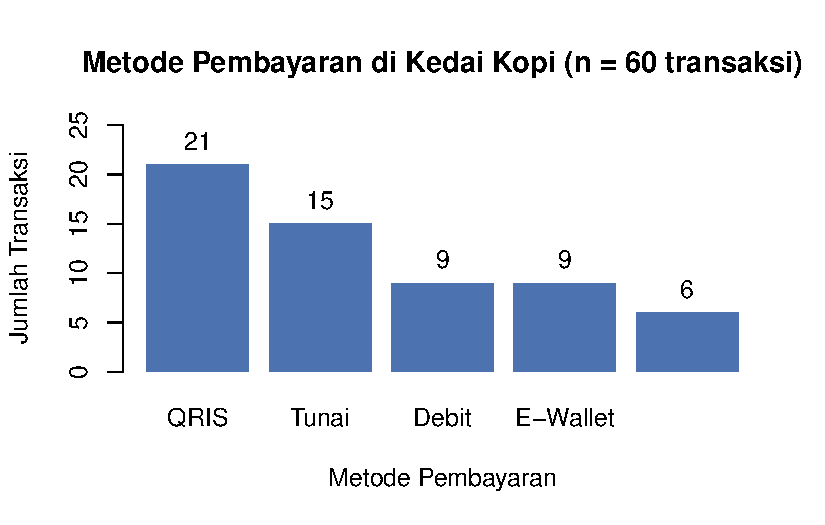
\includegraphics[keepaspectratio]{chapters/P04_files/figure-pdf/unnamed-chunk-9-1.pdf}}

Untuk nama kategori yang panjang atau banyak kategori, diagram batang
\textbf{horizontal} lebih mudah dibaca:

\begin{Shaded}
\begin{Highlighting}[]
\FunctionTok{par}\NormalTok{(}\AttributeTok{mar =} \FunctionTok{c}\NormalTok{(}\DecValTok{5}\NormalTok{, }\DecValTok{8}\NormalTok{, }\DecValTok{3}\NormalTok{, }\DecValTok{2}\NormalTok{))}
\FunctionTok{barplot}\NormalTok{(}\FunctionTok{rev}\NormalTok{(}\FunctionTok{prop.table}\NormalTok{(f\_metode) }\SpecialCharTok{*} \DecValTok{100}\NormalTok{), }\AttributeTok{horiz =} \ConstantTok{TRUE}\NormalTok{, }\AttributeTok{las =} \DecValTok{1}\NormalTok{, }\AttributeTok{col =} \StringTok{"\#4C72B0"}\NormalTok{, }\AttributeTok{border =} \ConstantTok{NA}\NormalTok{,}
\AttributeTok{xlab =} \StringTok{"Persentase Transaksi (\%)"}\NormalTok{, }\AttributeTok{main =} \StringTok{"Komposisi Metode Pembayaran"}\NormalTok{)}
\end{Highlighting}
\end{Shaded}

\pandocbounded{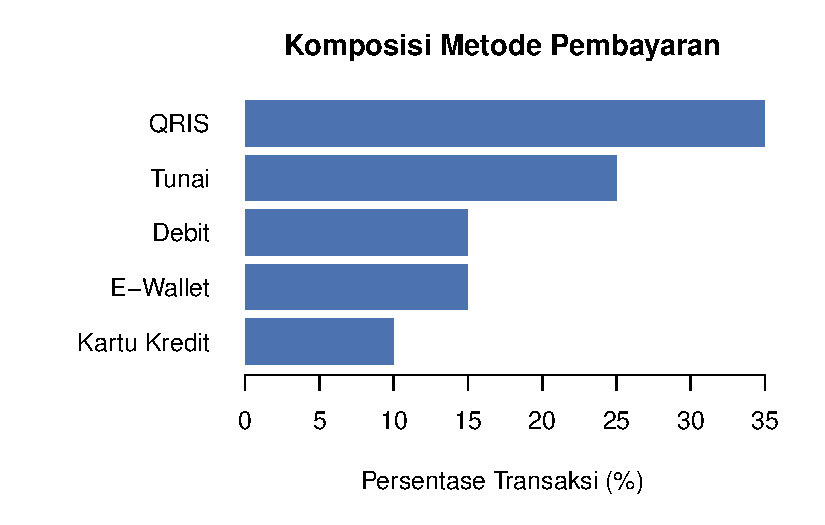
\includegraphics[keepaspectratio]{chapters/P04_files/figure-pdf/unnamed-chunk-10-1.pdf}}

\begin{Shaded}
\begin{Highlighting}[]
\FunctionTok{par}\NormalTok{(}\AttributeTok{mar =} \FunctionTok{c}\NormalTok{(}\DecValTok{5}\NormalTok{, }\DecValTok{4}\NormalTok{, }\DecValTok{4}\NormalTok{, }\DecValTok{2}\NormalTok{) }\SpecialCharTok{+} \FloatTok{0.1}\NormalTok{)}
\end{Highlighting}
\end{Shaded}

\subsection{Diagram Batang Berkelompok dan
Bertumpuk}\label{diagram-batang-berkelompok-dan-bertumpuk}

\begin{Shaded}
\begin{Highlighting}[]
\NormalTok{warna\_waktu }\OtherTok{\textless{}{-}} \FunctionTok{c}\NormalTok{(}\StringTok{"\#fdd49e"}\NormalTok{, }\StringTok{"\#fc8d59"}\NormalTok{, }\StringTok{"\#b30000"}\NormalTok{)}
\FunctionTok{par}\NormalTok{(}\AttributeTok{mfrow =} \FunctionTok{c}\NormalTok{(}\DecValTok{1}\NormalTok{, }\DecValTok{2}\NormalTok{))}
\FunctionTok{barplot}\NormalTok{(silang, }\AttributeTok{beside =} \ConstantTok{TRUE}\NormalTok{, }\AttributeTok{col =}\NormalTok{ warna\_waktu, }\AttributeTok{border =} \ConstantTok{NA}\NormalTok{, }\AttributeTok{las =} \DecValTok{2}\NormalTok{, }\AttributeTok{cex.names =} \FloatTok{0.75}\NormalTok{,}
\AttributeTok{main =} \StringTok{"Berkelompok (beside = TRUE)"}\NormalTok{, }\AttributeTok{ylab =} \StringTok{"Jumlah Transaksi"}\NormalTok{)}
\FunctionTok{legend}\NormalTok{(}\StringTok{"topright"}\NormalTok{, }\AttributeTok{legend =} \FunctionTok{rownames}\NormalTok{(silang), }\AttributeTok{fill =}\NormalTok{ warna\_waktu, }\AttributeTok{bty =} \StringTok{"n"}\NormalTok{, }\AttributeTok{cex =} \FloatTok{0.8}\NormalTok{)}
\FunctionTok{barplot}\NormalTok{(}\FunctionTok{prop.table}\NormalTok{(silang, }\AttributeTok{margin =} \DecValTok{2}\NormalTok{) }\SpecialCharTok{*} \DecValTok{100}\NormalTok{, }\AttributeTok{col =}\NormalTok{ warna\_waktu, }\AttributeTok{border =} \ConstantTok{NA}\NormalTok{, }\AttributeTok{las =} \DecValTok{2}\NormalTok{,}
\AttributeTok{cex.names =} \FloatTok{0.75}\NormalTok{, }\AttributeTok{main =} \StringTok{"Bertumpuk 100\%"}\NormalTok{, }\AttributeTok{ylab =} \StringTok{"Persentase (\%)"}\NormalTok{)}
\end{Highlighting}
\end{Shaded}

\pandocbounded{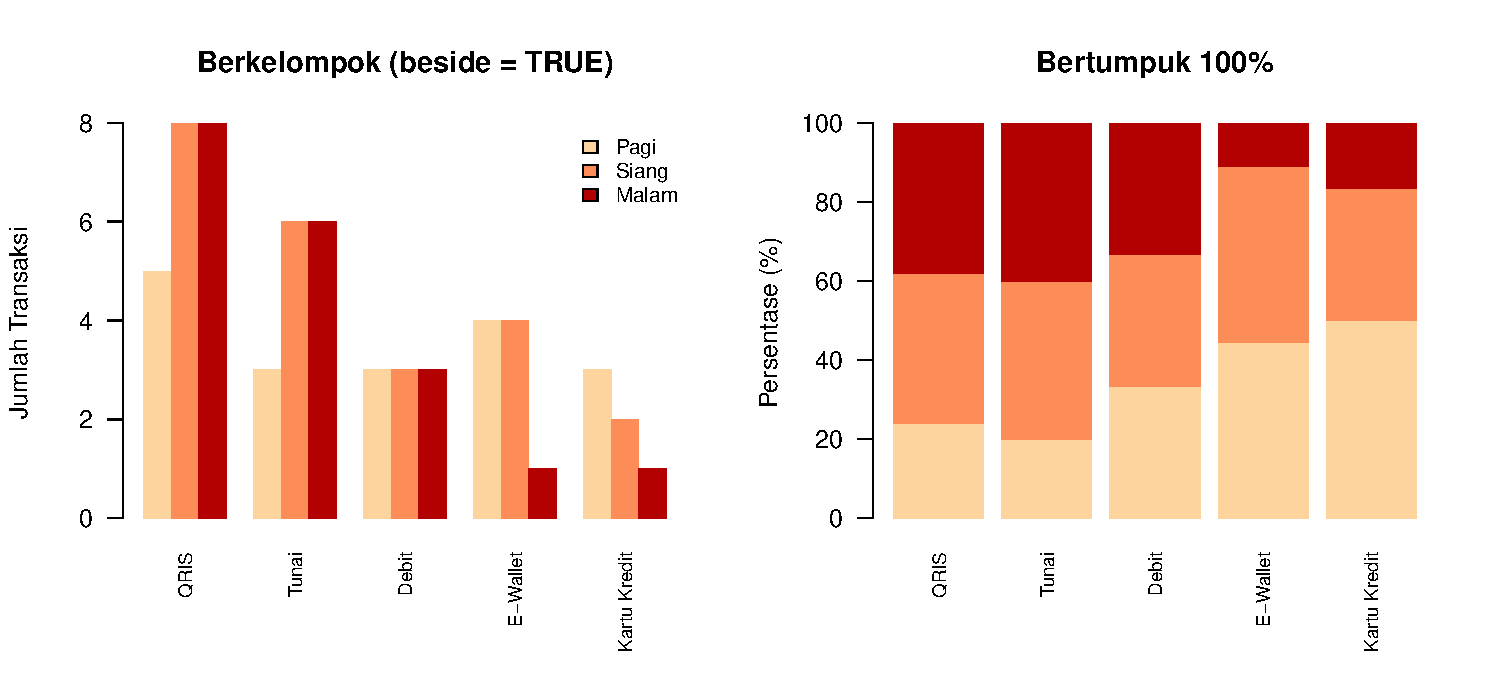
\includegraphics[keepaspectratio]{chapters/P04_files/figure-pdf/unnamed-chunk-11-1.pdf}}

\begin{Shaded}
\begin{Highlighting}[]
\FunctionTok{par}\NormalTok{(}\AttributeTok{mfrow =} \FunctionTok{c}\NormalTok{(}\DecValTok{1}\NormalTok{, }\DecValTok{1}\NormalTok{))}
\end{Highlighting}
\end{Shaded}

Diagram \textbf{berkelompok} baik untuk membandingkan frekuensi absolut;
diagram \textbf{bertumpuk 100\%} baik untuk membandingkan
\textbf{komposisi} antarkategori.

\subsection{Diagram Pareto}\label{diagram-pareto}

Diagram Pareto adalah diagram batang yang diurutkan dari frekuensi
terbesar, ditambah garis \textbf{persentase kumulatif}. Ia dipakai untuk
menemukan ``sedikit penyebab yang menyumbang sebagian besar masalah''
(prinsip 80/20), misalnya jenis keluhan pelanggan.

\begin{Shaded}
\begin{Highlighting}[]
\NormalTok{keluhan }\OtherTok{\textless{}{-}} \FunctionTok{c}\NormalTok{(}\StringTok{"Pengiriman terlambat"} \OtherTok{=} \DecValTok{48}\NormalTok{, }\StringTok{"Barang rusak"} \OtherTok{=} \DecValTok{27}\NormalTok{, }\StringTok{"Salah kirim"} \OtherTok{=} \DecValTok{14}\NormalTok{,}
\StringTok{"Refund lama"} \OtherTok{=} \DecValTok{7}\NormalTok{, }\StringTok{"CS tidak responsif"} \OtherTok{=} \DecValTok{5}\NormalTok{, }\StringTok{"Lainnya"} \OtherTok{=} \DecValTok{4}\NormalTok{)}
\NormalTok{kum\_persen }\OtherTok{\textless{}{-}} \FunctionTok{cumsum}\NormalTok{(keluhan) }\SpecialCharTok{/} \FunctionTok{sum}\NormalTok{(keluhan) }\SpecialCharTok{*} \DecValTok{100}

\FunctionTok{par}\NormalTok{(}\AttributeTok{mar =} \FunctionTok{c}\NormalTok{(}\DecValTok{8}\NormalTok{, }\DecValTok{4}\NormalTok{, }\DecValTok{3}\NormalTok{, }\DecValTok{4}\NormalTok{))}
\NormalTok{bp }\OtherTok{\textless{}{-}} \FunctionTok{barplot}\NormalTok{(keluhan, }\AttributeTok{col =} \StringTok{"\#DD8452"}\NormalTok{, }\AttributeTok{border =} \ConstantTok{NA}\NormalTok{, }\AttributeTok{las =} \DecValTok{2}\NormalTok{, }\AttributeTok{ylim =} \FunctionTok{c}\NormalTok{(}\DecValTok{0}\NormalTok{, }\FunctionTok{sum}\NormalTok{(keluhan)),}
\AttributeTok{ylab =} \StringTok{"Jumlah Keluhan"}\NormalTok{, }\AttributeTok{main =} \StringTok{"Diagram Pareto Keluhan Pelanggan"}\NormalTok{)}
\FunctionTok{lines}\NormalTok{(bp, kum\_persen }\SpecialCharTok{/} \DecValTok{100} \SpecialCharTok{*} \FunctionTok{sum}\NormalTok{(keluhan), }\AttributeTok{type =} \StringTok{"b"}\NormalTok{, }\AttributeTok{pch =} \DecValTok{16}\NormalTok{, }\AttributeTok{lwd =} \DecValTok{2}\NormalTok{)}
\FunctionTok{axis}\NormalTok{(}\DecValTok{4}\NormalTok{, }\AttributeTok{at =} \FunctionTok{seq}\NormalTok{(}\DecValTok{0}\NormalTok{, }\FunctionTok{sum}\NormalTok{(keluhan), }\AttributeTok{length.out =} \DecValTok{5}\NormalTok{), }\AttributeTok{labels =} \FunctionTok{paste0}\NormalTok{(}\FunctionTok{seq}\NormalTok{(}\DecValTok{0}\NormalTok{, }\DecValTok{100}\NormalTok{, }\DecValTok{25}\NormalTok{), }\StringTok{"\%"}\NormalTok{))}
\FunctionTok{abline}\NormalTok{(}\AttributeTok{h =} \FloatTok{0.8} \SpecialCharTok{*} \FunctionTok{sum}\NormalTok{(keluhan), }\AttributeTok{lty =} \DecValTok{2}\NormalTok{, }\AttributeTok{col =} \StringTok{"grey40"}\NormalTok{)}
\end{Highlighting}
\end{Shaded}

\pandocbounded{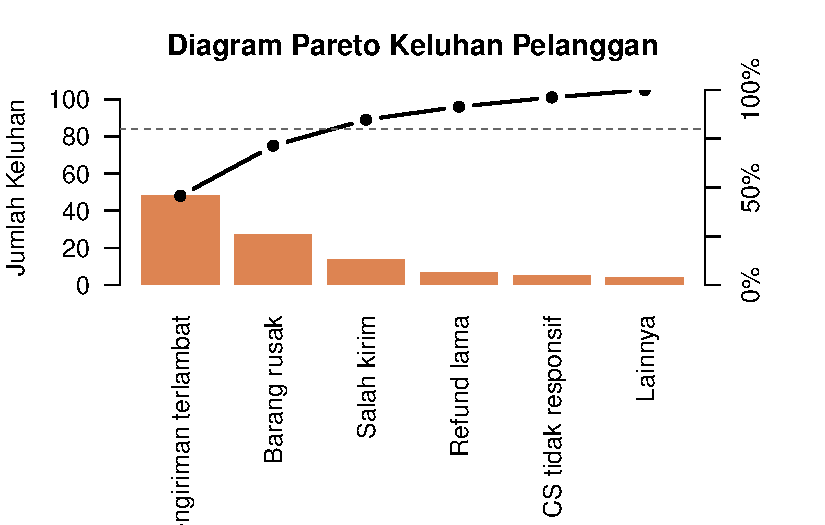
\includegraphics[keepaspectratio]{chapters/P04_files/figure-pdf/unnamed-chunk-12-1.pdf}}

\begin{Shaded}
\begin{Highlighting}[]
\FunctionTok{par}\NormalTok{(}\AttributeTok{mar =} \FunctionTok{c}\NormalTok{(}\DecValTok{5}\NormalTok{, }\DecValTok{4}\NormalTok{, }\DecValTok{4}\NormalTok{, }\DecValTok{2}\NormalTok{) }\SpecialCharTok{+} \FloatTok{0.1}\NormalTok{)}
\FunctionTok{round}\NormalTok{(kum\_persen, }\DecValTok{1}\NormalTok{)}
\end{Highlighting}
\end{Shaded}

\begin{verbatim}
Pengiriman terlambat         Barang rusak          Salah kirim 
                45.7                 71.4                 84.8 
         Refund lama   CS tidak responsif              Lainnya 
                91.4                 96.2                100.0 
\end{verbatim}

Dua jenis keluhan teratas sudah menyumbang 71.4\% dari seluruh keluhan
-- prioritas perbaikan yang jelas.

\subsection{Diagram Lingkaran (Pie
Chart)}\label{diagram-lingkaran-pie-chart}

Diagram lingkaran menunjukkan \textbf{bagian dari keseluruhan} (total
harus 100\%).

\begin{Shaded}
\begin{Highlighting}[]
\NormalTok{label\_pie }\OtherTok{\textless{}{-}} \FunctionTok{paste0}\NormalTok{(}\FunctionTok{names}\NormalTok{(f\_metode), }\StringTok{"}\SpecialCharTok{\textbackslash{}n}\StringTok{"}\NormalTok{, }\FunctionTok{round}\NormalTok{(}\FunctionTok{prop.table}\NormalTok{(f\_metode) }\SpecialCharTok{*} \DecValTok{100}\NormalTok{, }\DecValTok{1}\NormalTok{), }\StringTok{"\%"}\NormalTok{)}
\FunctionTok{pie}\NormalTok{(f\_metode, }\AttributeTok{labels =}\NormalTok{ label\_pie, }\AttributeTok{col =} \FunctionTok{c}\NormalTok{(}\StringTok{"\#4C72B0"}\NormalTok{, }\StringTok{"\#DD8452"}\NormalTok{, }\StringTok{"\#55A868"}\NormalTok{, }\StringTok{"\#C44E52"}\NormalTok{, }\StringTok{"\#8172B3"}\NormalTok{),}
\AttributeTok{border =} \StringTok{"white"}\NormalTok{, }\AttributeTok{main =} \StringTok{"Komposisi Metode Pembayaran"}\NormalTok{)}
\end{Highlighting}
\end{Shaded}

\pandocbounded{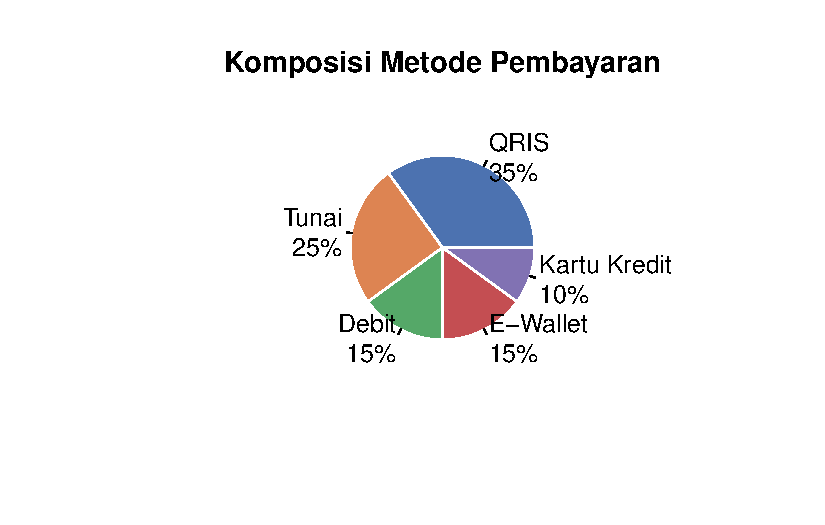
\includegraphics[keepaspectratio]{chapters/P04_files/figure-pdf/unnamed-chunk-13-1.pdf}}

\textbf{Kapan diagram lingkaran boleh dipakai?} Hanya jika (1)
kategorinya sedikit (sekitar 2--5), (2) proporsinya berbeda cukup jelas,
dan (3) pesannya adalah ``bagian dari keseluruhan''. Mata manusia lebih
pandai membandingkan \textbf{panjang} daripada \textbf{sudut}, sehingga
untuk perbandingan yang teliti, diagram batang hampir selalu lebih baik.

\begin{Shaded}
\begin{Highlighting}[]
\NormalTok{mirip }\OtherTok{\textless{}{-}} \FunctionTok{c}\NormalTok{(}\AttributeTok{A =} \DecValTok{21}\NormalTok{, }\AttributeTok{B =} \DecValTok{19}\NormalTok{, }\AttributeTok{C =} \DecValTok{20}\NormalTok{, }\AttributeTok{D =} \DecValTok{22}\NormalTok{, }\AttributeTok{E =} \DecValTok{18}\NormalTok{)}
\FunctionTok{par}\NormalTok{(}\AttributeTok{mfrow =} \FunctionTok{c}\NormalTok{(}\DecValTok{1}\NormalTok{, }\DecValTok{2}\NormalTok{))}
\FunctionTok{pie}\NormalTok{(mirip, }\AttributeTok{col =} \FunctionTok{hcl.colors}\NormalTok{(}\DecValTok{5}\NormalTok{, }\StringTok{"Set 2"}\NormalTok{), }\AttributeTok{main =} \StringTok{"Mana yang terbesar?"}\NormalTok{)}
\FunctionTok{barplot}\NormalTok{(mirip, }\AttributeTok{col =} \FunctionTok{hcl.colors}\NormalTok{(}\DecValTok{5}\NormalTok{, }\StringTok{"Set 2"}\NormalTok{), }\AttributeTok{border =} \ConstantTok{NA}\NormalTok{, }\AttributeTok{main =} \StringTok{"Sekarang jelas: D"}\NormalTok{)}
\end{Highlighting}
\end{Shaded}

\pandocbounded{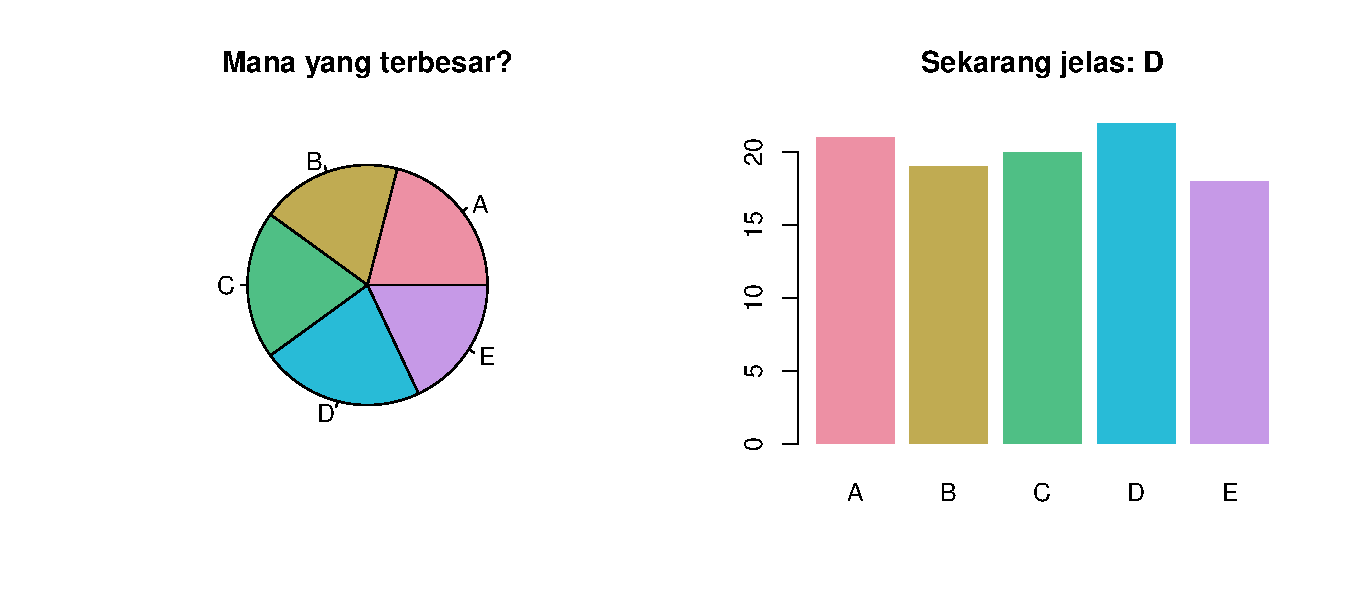
\includegraphics[keepaspectratio]{chapters/P04_files/figure-pdf/unnamed-chunk-14-1.pdf}}

\begin{Shaded}
\begin{Highlighting}[]
\FunctionTok{par}\NormalTok{(}\AttributeTok{mfrow =} \FunctionTok{c}\NormalTok{(}\DecValTok{1}\NormalTok{, }\DecValTok{1}\NormalTok{))}
\end{Highlighting}
\end{Shaded}

\section{Visualisasi Data Numerik}\label{visualisasi-data-numerik}

\subsection{Histogram}\label{histogram}

Histogram menampilkan distribusi data numerik yang
\textbf{dikelompokkan}. Berbeda dengan diagram batang, batang histogram
\textbf{saling menempel} karena kelasnya bersambung (sumbu-x adalah
skala numerik).

\begin{Shaded}
\begin{Highlighting}[]
\FunctionTok{hist}\NormalTok{(nilai\_ujian, }\AttributeTok{breaks =}\NormalTok{ batas\_nyata\_u, }\AttributeTok{col =} \StringTok{"\#4C72B0"}\NormalTok{, }\AttributeTok{border =} \StringTok{"white"}\NormalTok{,}
\AttributeTok{xaxt =} \StringTok{"n"}\NormalTok{, }\AttributeTok{ylim =} \FunctionTok{c}\NormalTok{(}\DecValTok{0}\NormalTok{, }\DecValTok{7}\NormalTok{),}
\AttributeTok{main =} \StringTok{"Histogram Nilai Ujian Statistika (n = 30)"}\NormalTok{, }\AttributeTok{xlab =} \StringTok{"Nilai Ujian"}\NormalTok{, }\AttributeTok{ylab =} \StringTok{"Frekuensi"}\NormalTok{)}
\FunctionTok{axis}\NormalTok{(}\DecValTok{1}\NormalTok{, }\AttributeTok{at =}\NormalTok{ batas\_nyata\_u)}
\end{Highlighting}
\end{Shaded}

\pandocbounded{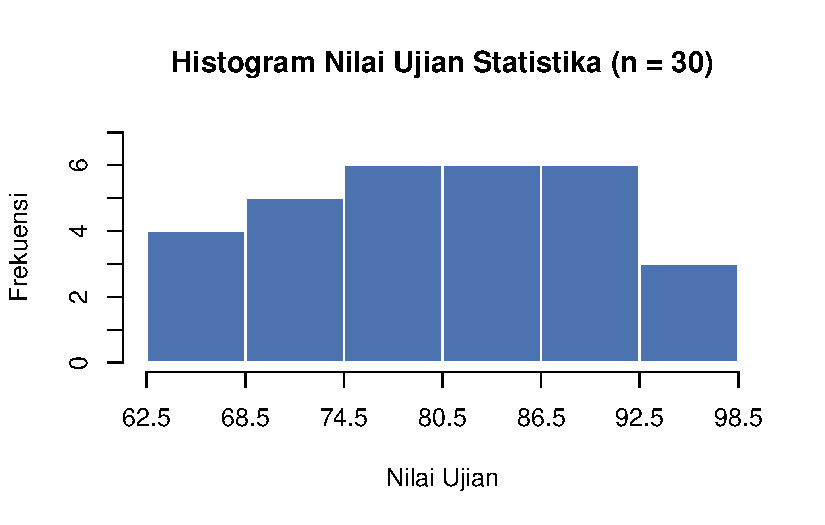
\includegraphics[keepaspectratio]{chapters/P04_files/figure-pdf/unnamed-chunk-15-1.pdf}}

{\def\LTcaptype{none} % do not increment counter
\begin{longtable}[]{@{}
  >{\raggedright\arraybackslash}p{(\linewidth - 4\tabcolsep) * \real{0.3333}}
  >{\raggedright\arraybackslash}p{(\linewidth - 4\tabcolsep) * \real{0.3333}}
  >{\raggedright\arraybackslash}p{(\linewidth - 4\tabcolsep) * \real{0.3333}}@{}}
\toprule\noalign{}
\begin{minipage}[b]{\linewidth}\raggedright
Aspek
\end{minipage} & \begin{minipage}[b]{\linewidth}\raggedright
Diagram Batang
\end{minipage} & \begin{minipage}[b]{\linewidth}\raggedright
Histogram
\end{minipage} \\
\midrule\noalign{}
\endhead
\bottomrule\noalign{}
\endlastfoot
Jenis data & Kategorik (atau diskrit dengan sedikit nilai) & Numerik
kontinu (atau diskrit dengan banyak nilai) \\
Sumbu-x & Kategori (urutan boleh diubah) & Skala numerik (urutan
tetap) \\
Celah antarbatang & Ada & Tidak ada \\
Lebar batang & Tidak bermakna & Mewakili lebar kelas \\
\end{longtable}
}

\subsection{Histogram dari Data
Terkelompok}\label{histogram-dari-data-terkelompok}

Jika hanya tabel yang tersedia, histogram digambar dari batas nyata dan
frekuensinya:

\begin{Shaded}
\begin{Highlighting}[]
\FunctionTok{plot}\NormalTok{(}\ConstantTok{NULL}\NormalTok{, }\AttributeTok{xlim =} \FunctionTok{range}\NormalTok{(batas\_nyata\_p), }\AttributeTok{ylim =} \FunctionTok{c}\NormalTok{(}\DecValTok{0}\NormalTok{, }\DecValTok{45}\NormalTok{), }\AttributeTok{xaxt =} \StringTok{"n"}\NormalTok{,}
\AttributeTok{xlab =} \StringTok{"Pendapatan Mingguan (USD)"}\NormalTok{, }\AttributeTok{ylab =} \StringTok{"Frekuensi"}\NormalTok{,}
\AttributeTok{main =} \StringTok{"Histogram Pendapatan Mingguan 100 Karyawan"}\NormalTok{)}
\FunctionTok{rect}\NormalTok{(L\_p, }\DecValTok{0}\NormalTok{, U\_p, f\_p, }\AttributeTok{col =} \StringTok{"\#9ecae1"}\NormalTok{, }\AttributeTok{border =} \StringTok{"white"}\NormalTok{)}
\FunctionTok{axis}\NormalTok{(}\DecValTok{1}\NormalTok{, }\AttributeTok{at =}\NormalTok{ batas\_nyata\_p, }\AttributeTok{labels =}\NormalTok{ batas\_nyata\_p)}
\FunctionTok{text}\NormalTok{((L\_p }\SpecialCharTok{+}\NormalTok{ U\_p) }\SpecialCharTok{/} \DecValTok{2}\NormalTok{, f\_p, }\AttributeTok{labels =}\NormalTok{ f\_p, }\AttributeTok{pos =} \DecValTok{3}\NormalTok{)}
\end{Highlighting}
\end{Shaded}

\pandocbounded{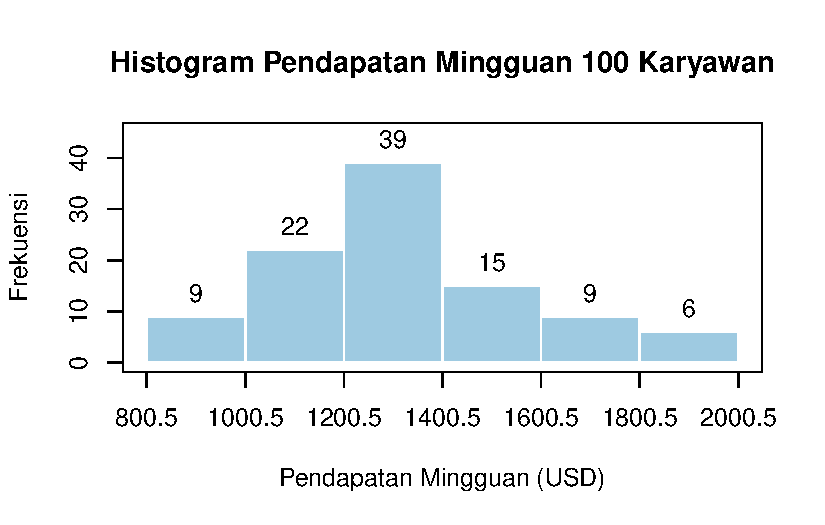
\includegraphics[keepaspectratio]{chapters/P04_files/figure-pdf/unnamed-chunk-16-1.pdf}}

Distribusi pendapatan \textbf{menjulur ke kanan}: puncak di kelas
1201--1400, dengan ekor panjang ke arah pendapatan tinggi.

\subsection{Poligon Frekuensi}\label{poligon-frekuensi}

Poligon frekuensi menghubungkan \textbf{titik tengah} puncak tiap kelas
dengan garis. Ditambahkan satu kelas kosong di kedua ujung agar poligon
``menapak'' di sumbu-x. Poligon berguna untuk \textbf{membandingkan}
beberapa distribusi dalam satu grafik.

\begin{Shaded}
\begin{Highlighting}[]
\NormalTok{m\_u }\OtherTok{\textless{}{-}}\NormalTok{ (}\FunctionTok{head}\NormalTok{(batas\_nyata\_u, }\SpecialCharTok{{-}}\DecValTok{1}\NormalTok{) }\SpecialCharTok{+} \FunctionTok{tail}\NormalTok{(batas\_nyata\_u, }\SpecialCharTok{{-}}\DecValTok{1}\NormalTok{)) }\SpecialCharTok{/} \DecValTok{2}
\NormalTok{x\_pol }\OtherTok{\textless{}{-}} \FunctionTok{c}\NormalTok{(}\FunctionTok{min}\NormalTok{(m\_u) }\SpecialCharTok{{-}}\NormalTok{ w, m\_u, }\FunctionTok{max}\NormalTok{(m\_u) }\SpecialCharTok{+}\NormalTok{ w)}
\NormalTok{y\_pol }\OtherTok{\textless{}{-}} \FunctionTok{c}\NormalTok{(}\DecValTok{0}\NormalTok{, f\_ujian, }\DecValTok{0}\NormalTok{)}

\FunctionTok{hist}\NormalTok{(nilai\_ujian, }\AttributeTok{breaks =}\NormalTok{ batas\_nyata\_u, }\AttributeTok{col =} \StringTok{"grey90"}\NormalTok{, }\AttributeTok{border =} \StringTok{"white"}\NormalTok{, }\AttributeTok{ylim =} \FunctionTok{c}\NormalTok{(}\DecValTok{0}\NormalTok{, }\DecValTok{7}\NormalTok{),}
\AttributeTok{xlim =} \FunctionTok{range}\NormalTok{(x\_pol), }\AttributeTok{main =} \StringTok{"Poligon Frekuensi Nilai Ujian"}\NormalTok{, }\AttributeTok{xlab =} \StringTok{"Nilai Ujian"}\NormalTok{,}
\AttributeTok{ylab =} \StringTok{"Frekuensi"}\NormalTok{)}
\FunctionTok{lines}\NormalTok{(x\_pol, y\_pol, }\AttributeTok{type =} \StringTok{"b"}\NormalTok{, }\AttributeTok{pch =} \DecValTok{16}\NormalTok{, }\AttributeTok{col =} \StringTok{"firebrick"}\NormalTok{, }\AttributeTok{lwd =} \DecValTok{2}\NormalTok{)}
\end{Highlighting}
\end{Shaded}

\pandocbounded{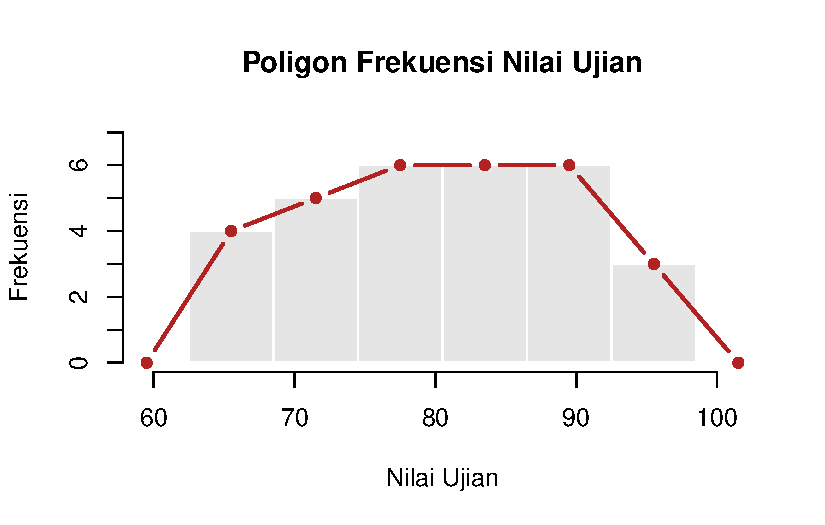
\includegraphics[keepaspectratio]{chapters/P04_files/figure-pdf/unnamed-chunk-17-1.pdf}}

\subsection{Ogive (Kurva Frekuensi
Kumulatif)}\label{ogive-kurva-frekuensi-kumulatif}

Ogive memplot \textbf{frekuensi kumulatif} terhadap \textbf{batas nyata
atas} tiap kelas (dimulai dari batas nyata bawah kelas pertama dengan
kumulatif 0). Ogive memudahkan menjawab ``berapa persen data di bawah
nilai tertentu?'' dan menaksir median secara grafis.

\begin{Shaded}
\begin{Highlighting}[]
\NormalTok{x\_ogive }\OtherTok{\textless{}{-}}\NormalTok{ batas\_nyata\_p}
\NormalTok{y\_ogive }\OtherTok{\textless{}{-}} \FunctionTok{c}\NormalTok{(}\DecValTok{0}\NormalTok{, }\FunctionTok{cumsum}\NormalTok{(f\_p)) }\SpecialCharTok{/}\NormalTok{ n\_p }\SpecialCharTok{*} \DecValTok{100}

\FunctionTok{plot}\NormalTok{(x\_ogive, y\_ogive, }\AttributeTok{type =} \StringTok{"b"}\NormalTok{, }\AttributeTok{pch =} \DecValTok{16}\NormalTok{, }\AttributeTok{lwd =} \DecValTok{2}\NormalTok{, }\AttributeTok{col =} \StringTok{"\#4C72B0"}\NormalTok{, }\AttributeTok{ylim =} \FunctionTok{c}\NormalTok{(}\DecValTok{0}\NormalTok{, }\DecValTok{100}\NormalTok{),}
\AttributeTok{xaxt =} \StringTok{"n"}\NormalTok{, }\AttributeTok{xlab =} \StringTok{"Pendapatan Mingguan (USD)"}\NormalTok{, }\AttributeTok{ylab =} \StringTok{"Persentase Kumulatif (\%)"}\NormalTok{,}
\AttributeTok{main =} \StringTok{"Ogive \textquotesingle{}Kurang Dari\textquotesingle{} Pendapatan Mingguan"}\NormalTok{)}
\FunctionTok{axis}\NormalTok{(}\DecValTok{1}\NormalTok{, }\AttributeTok{at =}\NormalTok{ batas\_nyata\_p)}
\FunctionTok{abline}\NormalTok{(}\AttributeTok{h =} \DecValTok{50}\NormalTok{, }\AttributeTok{lty =} \DecValTok{2}\NormalTok{, }\AttributeTok{col =} \StringTok{"grey40"}\NormalTok{)}
\NormalTok{median\_grafis }\OtherTok{\textless{}{-}} \FunctionTok{approx}\NormalTok{(y\_ogive, x\_ogive, }\AttributeTok{xout =} \DecValTok{50}\NormalTok{)}\SpecialCharTok{$}\NormalTok{y}
\FunctionTok{abline}\NormalTok{(}\AttributeTok{v =}\NormalTok{ median\_grafis, }\AttributeTok{lty =} \DecValTok{2}\NormalTok{, }\AttributeTok{col =} \StringTok{"firebrick"}\NormalTok{)}
\FunctionTok{text}\NormalTok{(median\_grafis, }\DecValTok{8}\NormalTok{, }\AttributeTok{labels =} \FunctionTok{paste0}\NormalTok{(}\StringTok{"\textasciitilde{}"}\NormalTok{, }\FunctionTok{round}\NormalTok{(median\_grafis)), }\AttributeTok{pos =} \DecValTok{4}\NormalTok{, }\AttributeTok{col =} \StringTok{"firebrick"}\NormalTok{)}
\end{Highlighting}
\end{Shaded}

\pandocbounded{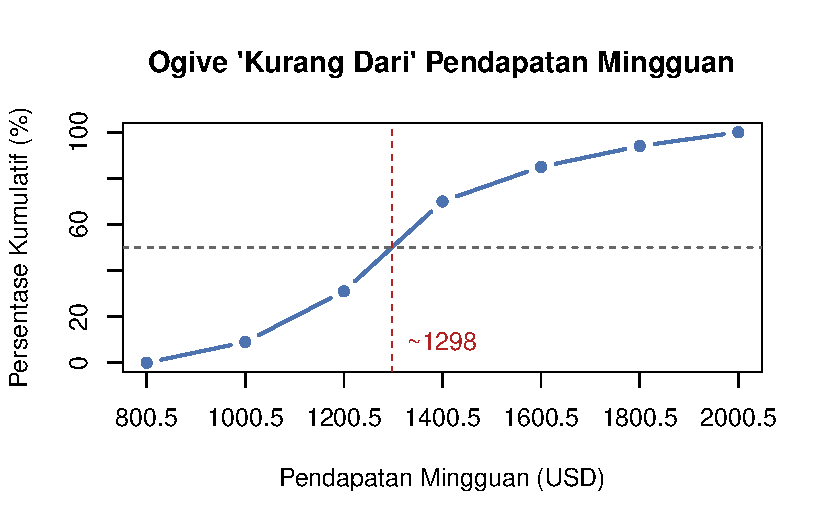
\includegraphics[keepaspectratio]{chapters/P04_files/figure-pdf/unnamed-chunk-18-1.pdf}}

Garis 50\% memotong ogive di sekitar \textbf{1298 USD} -- inilah
taksiran median secara grafis. Pada Pertemuan 5 kita akan menghitung
median data terkelompok secara aljabar dan mendapatkan angka yang sama.

\subsection{Diagram Batang-Daun
(Stem-and-Leaf)}\label{diagram-batang-daun-stem-and-leaf}

Diagram batang-daun memecah setiap nilai menjadi \textbf{batang} (digit
depan) dan \textbf{daun} (digit terakhir). Kelebihannya: bentuk
distribusi terlihat seperti histogram, tetapi \textbf{nilai asli tetap
terbaca}. Cocok untuk data berukuran kecil--sedang.

\begin{Shaded}
\begin{Highlighting}[]
\FunctionTok{stem}\NormalTok{(nilai\_ujian)}
\end{Highlighting}
\end{Shaded}

\begin{verbatim}

  The decimal point is 1 digit(s) to the right of the |

  6 | 3
  6 | 5789
  7 | 0124
  7 | 56789
  8 | 01234
  8 | 56789
  9 | 01234
  9 | 5
\end{verbatim}

Baca baris \texttt{7\ \textbar{}\ 0124} sebagai nilai 70, 71, 72, 74.
Perhatikan bahwa R otomatis memecah setiap batang menjadi dua baris
(daun 0--4 dan daun 5--9) agar bentuk distribusi lebih terlihat. Argumen
\texttt{scale} mengatur tingkat pemecahan tersebut;
\texttt{scale\ =\ 0.5} menghasilkan satu baris per puluhan:

\begin{Shaded}
\begin{Highlighting}[]
\FunctionTok{stem}\NormalTok{(nilai\_ujian, }\AttributeTok{scale =} \FloatTok{0.5}\NormalTok{)}
\end{Highlighting}
\end{Shaded}

\begin{verbatim}

  The decimal point is 1 digit(s) to the right of the |

  6 | 35789
  7 | 012456789
  8 | 0123456789
  9 | 012345
\end{verbatim}

Versi satu baris per puluhan lebih ringkas, tetapi bentuk distribusinya
menjadi kurang terlihat -- mirip histogram dengan kelas yang terlalu
lebar.

\subsection{Memilih Grafik yang Tepat}\label{memilih-grafik-yang-tepat}

{\def\LTcaptype{none} % do not increment counter
\begin{longtable}[]{@{}
  >{\raggedright\arraybackslash}p{(\linewidth - 2\tabcolsep) * \real{0.5000}}
  >{\raggedright\arraybackslash}p{(\linewidth - 2\tabcolsep) * \real{0.5000}}@{}}
\toprule\noalign{}
\begin{minipage}[b]{\linewidth}\raggedright
Tujuan / Jenis Data
\end{minipage} & \begin{minipage}[b]{\linewidth}\raggedright
Grafik yang disarankan
\end{minipage} \\
\midrule\noalign{}
\endhead
\bottomrule\noalign{}
\endlastfoot
Frekuensi kategori (nominal/ordinal) & Diagram batang (horizontal bila
label panjang) \\
Bagian dari keseluruhan, sedikit kategori & Diagram lingkaran atau
batang bertumpuk 100\% \\
Prioritas masalah & Diagram Pareto \\
Hubungan dua variabel kategorik & Batang berkelompok / bertumpuk; tabel
silang \\
Distribusi numerik (n besar) & Histogram \\
Distribusi numerik (n kecil) & Stem-and-leaf, diagram titik
(\texttt{stripchart}) \\
Membandingkan beberapa distribusi & Poligon frekuensi, boxplot
(Pertemuan 6) \\
Persentase di bawah suatu nilai & Ogive \\
\end{longtable}
}

\section{Prinsip Visualisasi yang
Jujur}\label{prinsip-visualisasi-yang-jujur}

\subsection{Prinsip 1 -- Skala: Jangan Memotong Sumbu Diagram
Batang}\label{prinsip-1-skala-jangan-memotong-sumbu-diagram-batang}

Panjang batang harus sebanding dengan nilainya. Jika sumbu-y tidak
dimulai dari nol, perbedaan kecil tampak raksasa.

\begin{Shaded}
\begin{Highlighting}[]
\NormalTok{pangsa }\OtherTok{\textless{}{-}} \FunctionTok{c}\NormalTok{(}\StringTok{"Aplikasi A"} \OtherTok{=} \DecValTok{41}\NormalTok{, }\StringTok{"Aplikasi B"} \OtherTok{=} \DecValTok{43}\NormalTok{)}
\FunctionTok{par}\NormalTok{(}\AttributeTok{mfrow =} \FunctionTok{c}\NormalTok{(}\DecValTok{1}\NormalTok{, }\DecValTok{2}\NormalTok{))}
\FunctionTok{barplot}\NormalTok{(pangsa, }\AttributeTok{ylim =} \FunctionTok{c}\NormalTok{(}\DecValTok{40}\NormalTok{, }\FloatTok{43.5}\NormalTok{), }\AttributeTok{xpd =} \ConstantTok{FALSE}\NormalTok{, }\AttributeTok{col =} \FunctionTok{c}\NormalTok{(}\StringTok{"grey60"}\NormalTok{, }\StringTok{"\#C44E52"}\NormalTok{),}
\AttributeTok{main =} \StringTok{"MENYESATKAN: sumbu mulai dari 40"}\NormalTok{, }\AttributeTok{ylab =} \StringTok{"Pangsa pasar (\%)"}\NormalTok{)}
\FunctionTok{box}\NormalTok{()}
\FunctionTok{barplot}\NormalTok{(pangsa, }\AttributeTok{ylim =} \FunctionTok{c}\NormalTok{(}\DecValTok{0}\NormalTok{, }\DecValTok{50}\NormalTok{), }\AttributeTok{col =} \FunctionTok{c}\NormalTok{(}\StringTok{"grey60"}\NormalTok{, }\StringTok{"\#C44E52"}\NormalTok{),}
\AttributeTok{main =} \StringTok{"JUJUR: sumbu mulai dari 0"}\NormalTok{, }\AttributeTok{ylab =} \StringTok{"Pangsa pasar (\%)"}\NormalTok{)}
\end{Highlighting}
\end{Shaded}

\pandocbounded{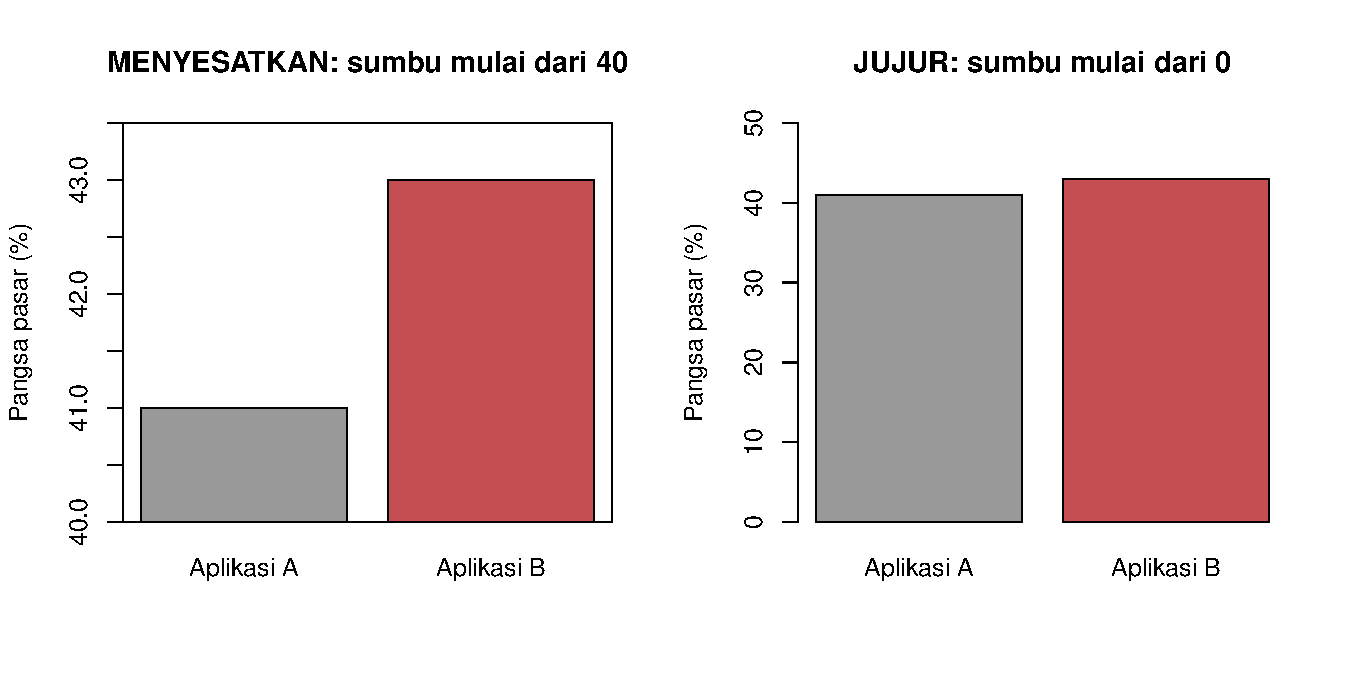
\includegraphics[keepaspectratio]{chapters/P04_files/figure-pdf/unnamed-chunk-21-1.pdf}}

\begin{Shaded}
\begin{Highlighting}[]
\FunctionTok{par}\NormalTok{(}\AttributeTok{mfrow =} \FunctionTok{c}\NormalTok{(}\DecValTok{1}\NormalTok{, }\DecValTok{1}\NormalTok{))}
\end{Highlighting}
\end{Shaded}

Grafik kiri membuat Aplikasi B tampak ``tiga kali'' lebih besar, padahal
selisihnya hanya 2 poin persentase. \textbf{Diagram garis} untuk tren
boleh tidak dimulai dari nol (yang dibaca adalah perubahan), tetapi
\textbf{diagram batang wajib dimulai dari nol}.

\subsection{Prinsip 2 -- Label: Grafik Harus Dapat Berdiri
Sendiri}\label{prinsip-2-label-grafik-harus-dapat-berdiri-sendiri}

Setiap grafik minimal memuat: \textbf{judul} yang informatif,
\textbf{label sumbu beserta satuan}, \textbf{legenda} bila ada lebih
dari satu kelompok, serta \textbf{sumber data dan} \(n\).

\begin{Shaded}
\begin{Highlighting}[]
\FunctionTok{par}\NormalTok{(}\AttributeTok{mfrow =} \FunctionTok{c}\NormalTok{(}\DecValTok{1}\NormalTok{, }\DecValTok{2}\NormalTok{))}
\FunctionTok{hist}\NormalTok{(nilai\_ujian, }\AttributeTok{breaks =}\NormalTok{ batas\_nyata\_u, }\AttributeTok{main =} \StringTok{""}\NormalTok{, }\AttributeTok{xlab =} \StringTok{""}\NormalTok{, }\AttributeTok{ylab =} \StringTok{""}\NormalTok{)}
\FunctionTok{hist}\NormalTok{(nilai\_ujian, }\AttributeTok{breaks =}\NormalTok{ batas\_nyata\_u, }\AttributeTok{col =} \StringTok{"\#4C72B0"}\NormalTok{, }\AttributeTok{border =} \StringTok{"white"}\NormalTok{,}
\AttributeTok{main =} \StringTok{"Nilai Ujian Statistika Kelas A}\SpecialCharTok{\textbackslash{}n}\StringTok{(n = 30, Semester Ganjil)"}\NormalTok{,}
\AttributeTok{xlab =} \StringTok{"Nilai Ujian (skala 0{-}100)"}\NormalTok{, }\AttributeTok{ylab =} \StringTok{"Jumlah Mahasiswa"}\NormalTok{)}
\end{Highlighting}
\end{Shaded}

\pandocbounded{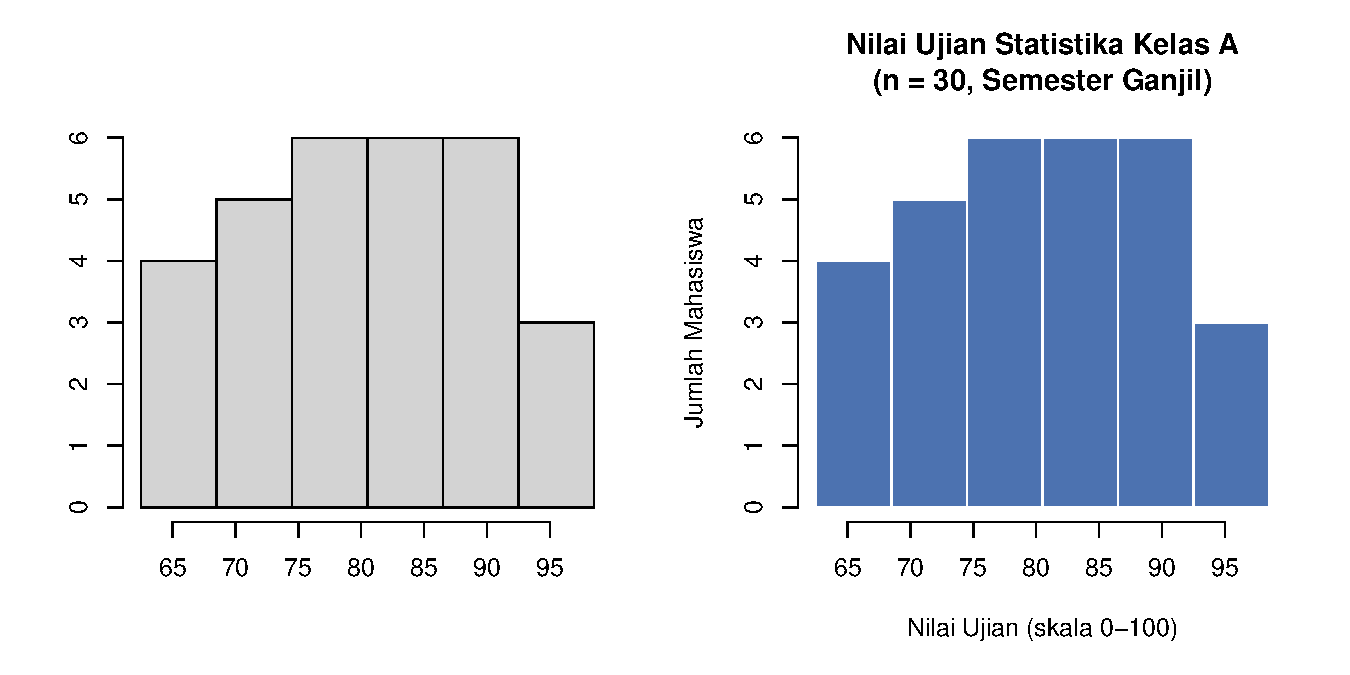
\includegraphics[keepaspectratio]{chapters/P04_files/figure-pdf/unnamed-chunk-22-1.pdf}}

\begin{Shaded}
\begin{Highlighting}[]
\FunctionTok{par}\NormalTok{(}\AttributeTok{mfrow =} \FunctionTok{c}\NormalTok{(}\DecValTok{1}\NormalTok{, }\DecValTok{1}\NormalTok{))}
\end{Highlighting}
\end{Shaded}

\subsection{Prinsip 3 -- Bin: Lebar Kelas Mengubah
Cerita}\label{prinsip-3-bin-lebar-kelas-mengubah-cerita}

Bentuk histogram sangat bergantung pada banyak kelas (\emph{bin}).
Terlalu sedikit kelas menyembunyikan pola; terlalu banyak kelas membuat
grafik ``bergerigi'' oleh kebetulan.

\begin{Shaded}
\begin{Highlighting}[]
\FunctionTok{set.seed}\NormalTok{(}\DecValTok{7}\NormalTok{)}
\NormalTok{waktu\_layanan }\OtherTok{\textless{}{-}} \FunctionTok{c}\NormalTok{(}\FunctionTok{rnorm}\NormalTok{(}\DecValTok{120}\NormalTok{, }\DecValTok{8}\NormalTok{, }\FloatTok{1.5}\NormalTok{), }\FunctionTok{rnorm}\NormalTok{(}\DecValTok{80}\NormalTok{, }\DecValTok{15}\NormalTok{, }\DecValTok{2}\NormalTok{)) }\CommentTok{\# dua jenis layanan tercampur}

\FunctionTok{par}\NormalTok{(}\AttributeTok{mfrow =} \FunctionTok{c}\NormalTok{(}\DecValTok{1}\NormalTok{, }\DecValTok{3}\NormalTok{))}
\FunctionTok{hist}\NormalTok{(waktu\_layanan, }\AttributeTok{breaks =} \DecValTok{3}\NormalTok{, }\AttributeTok{col =} \StringTok{"\#9ecae1"}\NormalTok{, }\AttributeTok{border =} \StringTok{"white"}\NormalTok{, }\AttributeTok{main =} \StringTok{"Terlalu sedikit (\textasciitilde{}3 kelas)"}\NormalTok{,}
\AttributeTok{xlab =} \StringTok{"Waktu layanan (menit)"}\NormalTok{)}
\FunctionTok{hist}\NormalTok{(waktu\_layanan, }\AttributeTok{breaks =} \FunctionTok{nclass.Sturges}\NormalTok{(waktu\_layanan), }\AttributeTok{col =} \StringTok{"\#4C72B0"}\NormalTok{, }\AttributeTok{border =} \StringTok{"white"}\NormalTok{,}
\AttributeTok{main =} \FunctionTok{paste0}\NormalTok{(}\StringTok{"Sturges ("}\NormalTok{, }\FunctionTok{nclass.Sturges}\NormalTok{(waktu\_layanan), }\StringTok{" kelas)"}\NormalTok{), }\AttributeTok{xlab =} \StringTok{"Waktu layanan (menit)"}\NormalTok{)}
\FunctionTok{hist}\NormalTok{(waktu\_layanan, }\AttributeTok{breaks =} \DecValTok{60}\NormalTok{, }\AttributeTok{col =} \StringTok{"\#9ecae1"}\NormalTok{, }\AttributeTok{border =} \StringTok{"white"}\NormalTok{, }\AttributeTok{main =} \StringTok{"Terlalu banyak (\textasciitilde{}60 kelas)"}\NormalTok{,}
\AttributeTok{xlab =} \StringTok{"Waktu layanan (menit)"}\NormalTok{)}
\end{Highlighting}
\end{Shaded}

\pandocbounded{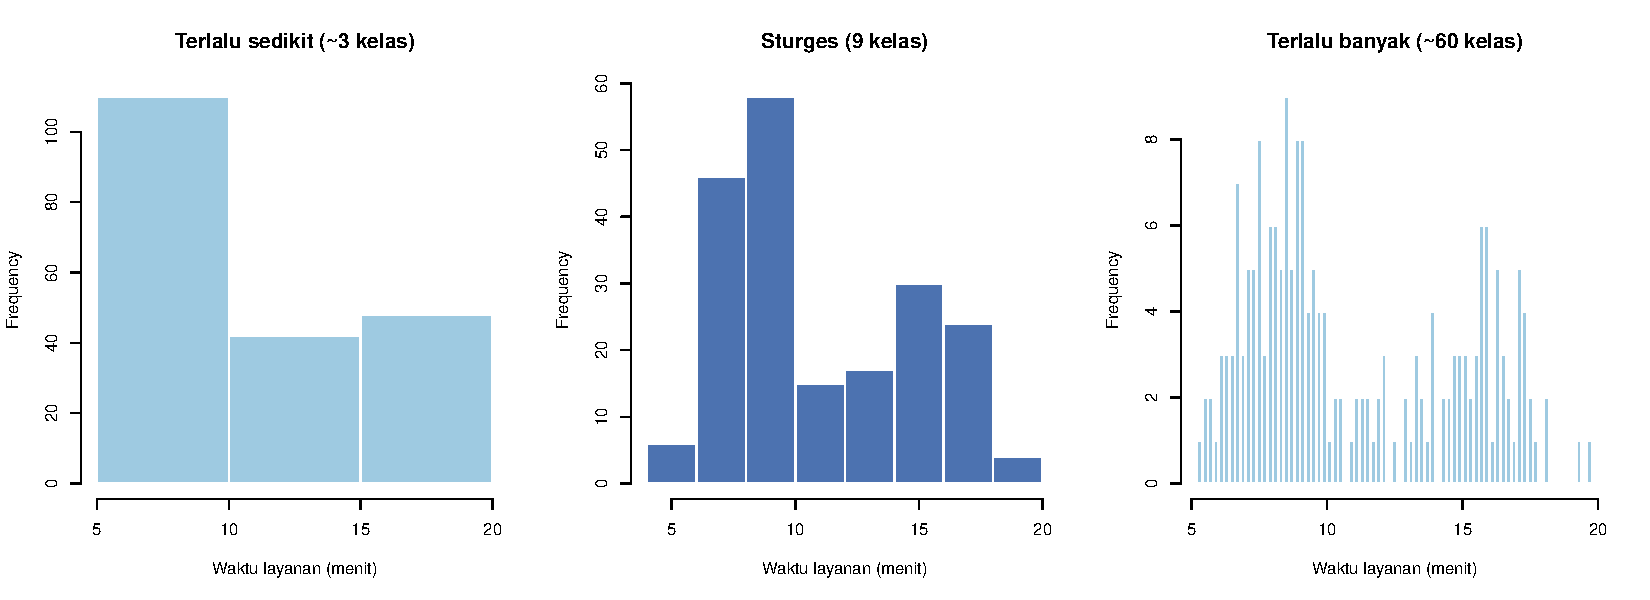
\includegraphics[keepaspectratio]{chapters/P04_files/figure-pdf/unnamed-chunk-23-1.pdf}}

\begin{Shaded}
\begin{Highlighting}[]
\FunctionTok{par}\NormalTok{(}\AttributeTok{mfrow =} \FunctionTok{c}\NormalTok{(}\DecValTok{1}\NormalTok{, }\DecValTok{1}\NormalTok{))}
\end{Highlighting}
\end{Shaded}

Dengan 3 kelas, dua puncak (dua jenis layanan) \textbf{tidak terlihat}.
Dengan 60 kelas, grafik penuh ``gigi'' acak. Aturan Sturges adalah titik
awal yang baik untuk \(n\) kecil--sedang, tetapi \textbf{selalu coba
beberapa pilihan} dan laporkan yang paling jujur menggambarkan data.
Untuk \(n\) besar, aturan lain seperti Freedman--Diaconis
(\texttt{nclass.FD()}) sering lebih baik.

\begin{Shaded}
\begin{Highlighting}[]
\FunctionTok{c}\NormalTok{(}\AttributeTok{Sturges =} \FunctionTok{nclass.Sturges}\NormalTok{(waktu\_layanan), }\AttributeTok{Scott =} \FunctionTok{nclass.scott}\NormalTok{(waktu\_layanan),}
\AttributeTok{Freedman\_Diaconis =} \FunctionTok{nclass.FD}\NormalTok{(waktu\_layanan))}
\end{Highlighting}
\end{Shaded}

\begin{verbatim}
          Sturges             Scott Freedman_Diaconis 
                9                 7                 7 
\end{verbatim}

\subsection{Prinsip 4 -- Interpretasi: Ceritakan Bentuk, Pusat, Sebaran,
dan
Keanehan}\label{prinsip-4-interpretasi-ceritakan-bentuk-pusat-sebaran-dan-keanehan}

Saat membaca histogram, biasakan menjawab empat hal:

{\def\LTcaptype{none} % do not increment counter
\begin{longtable}[]{@{}
  >{\raggedright\arraybackslash}p{(\linewidth - 4\tabcolsep) * \real{0.3333}}
  >{\raggedright\arraybackslash}p{(\linewidth - 4\tabcolsep) * \real{0.3333}}
  >{\raggedright\arraybackslash}p{(\linewidth - 4\tabcolsep) * \real{0.3333}}@{}}
\toprule\noalign{}
\begin{minipage}[b]{\linewidth}\raggedright
Aspek
\end{minipage} & \begin{minipage}[b]{\linewidth}\raggedright
Pertanyaan
\end{minipage} & \begin{minipage}[b]{\linewidth}\raggedright
Contoh untuk nilai ujian
\end{minipage} \\
\midrule\noalign{}
\endhead
\bottomrule\noalign{}
\endlastfoot
\textbf{Bentuk} & Simetris, menjulur kanan/kiri, satu atau dua puncak? &
Relatif simetris, satu puncak lebar \\
\textbf{Pusat} & Di sekitar nilai berapa data berkumpul? & Sekitar 80 \\
\textbf{Sebaran} & Dari berapa sampai berapa? Rapat atau menyebar? & 63
sampai 95, cukup merata \\
\textbf{Keanehan} & Ada celah, nilai ekstrem (outlier)? & Tidak tampak
outlier \\
\end{longtable}
}

Ukuran pusat dan sebaran secara numerik dibahas pada Pertemuan 5; bentuk
distribusi dan outlier secara formal pada Pertemuan 6.

\subsection{Grafik Menyesatkan
Lainnya}\label{grafik-menyesatkan-lainnya}

{\def\LTcaptype{none} % do not increment counter
\begin{longtable}[]{@{}
  >{\raggedright\arraybackslash}p{(\linewidth - 4\tabcolsep) * \real{0.3333}}
  >{\raggedright\arraybackslash}p{(\linewidth - 4\tabcolsep) * \real{0.3333}}
  >{\raggedright\arraybackslash}p{(\linewidth - 4\tabcolsep) * \real{0.3333}}@{}}
\toprule\noalign{}
\begin{minipage}[b]{\linewidth}\raggedright
Praktik menyesatkan
\end{minipage} & \begin{minipage}[b]{\linewidth}\raggedright
Mengapa menyesatkan
\end{minipage} & \begin{minipage}[b]{\linewidth}\raggedright
Perbaikan
\end{minipage} \\
\midrule\noalign{}
\endhead
\bottomrule\noalign{}
\endlastfoot
Diagram lingkaran dengan total ≠ 100\% & Irisan tidak mewakili bagian
dari keseluruhan & Gunakan diagram batang \\
Efek 3D, bayangan, gambar ikon yang diperbesar dua dimensi & Luas/volume
melebih-lebihkan perbedaan & Gunakan grafik 2D sederhana \\
Lebar kelas histogram tidak sama tanpa penyesuaian & Kelas lebar tampak
lebih ``penting'' & Gunakan lebar sama, atau plot kepadatan
(\texttt{freq\ =\ FALSE}) \\
Memilih rentang waktu yang menguntungkan (\emph{cherry picking}) & Tren
sesaat disajikan sebagai tren umum & Tampilkan periode yang utuh \\
Dua sumbu-y dengan skala berbeda & Korelasi palsu tampak meyakinkan &
Pisahkan menjadi dua grafik \\
\end{longtable}
}

\section{Studi Kasus Komprehensif: Waktu Pengiriman
Paket}\label{studi-kasus-komprehensif-waktu-pengiriman-paket}

\textbf{Konteks:} Sebuah layanan logistik mencatat waktu pengiriman
(jam, dari pemesanan hingga diterima) untuk 80 paket di wilayah Bekasi.
Manajer meminta laporan distribusi waktu pengiriman beserta komposisi
layanan yang dipakai.

\begin{Shaded}
\begin{Highlighting}[]
\FunctionTok{set.seed}\NormalTok{(}\DecValTok{2026}\NormalTok{)}
\NormalTok{layanan }\OtherTok{\textless{}{-}} \FunctionTok{sample}\NormalTok{(}\FunctionTok{c}\NormalTok{(}\StringTok{"Reguler"}\NormalTok{, }\StringTok{"Ekspres"}\NormalTok{, }\StringTok{"Same Day"}\NormalTok{), }\DecValTok{80}\NormalTok{, }\AttributeTok{replace =} \ConstantTok{TRUE}\NormalTok{, }\AttributeTok{prob =} \FunctionTok{c}\NormalTok{(}\FloatTok{0.55}\NormalTok{, }\FloatTok{0.30}\NormalTok{, }\FloatTok{0.15}\NormalTok{))}
\NormalTok{jam\_kirim }\OtherTok{\textless{}{-}} \FunctionTok{round}\NormalTok{(}\FunctionTok{ifelse}\NormalTok{(layanan }\SpecialCharTok{==} \StringTok{"Same Day"}\NormalTok{, }\FunctionTok{rnorm}\NormalTok{(}\DecValTok{80}\NormalTok{, }\DecValTok{6}\NormalTok{, }\FloatTok{1.5}\NormalTok{),}
\FunctionTok{ifelse}\NormalTok{(layanan }\SpecialCharTok{==} \StringTok{"Ekspres"}\NormalTok{, }\FunctionTok{rnorm}\NormalTok{(}\DecValTok{80}\NormalTok{, }\DecValTok{22}\NormalTok{, }\DecValTok{4}\NormalTok{), }\FunctionTok{rnorm}\NormalTok{(}\DecValTok{80}\NormalTok{, }\DecValTok{46}\NormalTok{, }\DecValTok{9}\NormalTok{))), }\DecValTok{1}\NormalTok{)}
\NormalTok{jam\_kirim }\OtherTok{\textless{}{-}} \FunctionTok{pmax}\NormalTok{(jam\_kirim, }\DecValTok{2}\NormalTok{)}
\FunctionTok{summary}\NormalTok{(jam\_kirim)}
\end{Highlighting}
\end{Shaded}

\begin{verbatim}
   Min. 1st Qu.  Median    Mean 3rd Qu.    Max. 
   3.10   22.38   38.90   34.92   48.62   65.50 
\end{verbatim}

\subsection{Langkah 1: Komposisi
Layanan}\label{langkah-1-komposisi-layanan}

\begin{Shaded}
\begin{Highlighting}[]
\NormalTok{f\_layanan }\OtherTok{\textless{}{-}} \FunctionTok{table}\NormalTok{(}\FunctionTok{factor}\NormalTok{(layanan, }\AttributeTok{levels =} \FunctionTok{c}\NormalTok{(}\StringTok{"Same Day"}\NormalTok{, }\StringTok{"Ekspres"}\NormalTok{, }\StringTok{"Reguler"}\NormalTok{)))}
\NormalTok{knitr}\SpecialCharTok{::}\FunctionTok{kable}\NormalTok{(}\FunctionTok{data.frame}\NormalTok{(}\AttributeTok{Layanan =} \FunctionTok{names}\NormalTok{(f\_layanan), }\AttributeTok{f =} \FunctionTok{as.numeric}\NormalTok{(f\_layanan),}
\AttributeTok{Persen =} \FunctionTok{round}\NormalTok{(}\FunctionTok{as.numeric}\NormalTok{(}\FunctionTok{prop.table}\NormalTok{(f\_layanan)) }\SpecialCharTok{*} \DecValTok{100}\NormalTok{, }\DecValTok{1}\NormalTok{)),}
\AttributeTok{caption =} \StringTok{"Komposisi Layanan Pengiriman (n = 80)"}\NormalTok{)}
\end{Highlighting}
\end{Shaded}

\begin{longtable}[]{@{}lrr@{}}
\caption{Komposisi Layanan Pengiriman (n = 80)}\tabularnewline
\toprule\noalign{}
Layanan & f & Persen \\
\midrule\noalign{}
\endfirsthead
\toprule\noalign{}
Layanan & f & Persen \\
\midrule\noalign{}
\endhead
\bottomrule\noalign{}
\endlastfoot
Same Day & 12 & 15 \\
Ekspres & 20 & 25 \\
Reguler & 48 & 60 \\
\end{longtable}

\begin{Shaded}
\begin{Highlighting}[]
\FunctionTok{barplot}\NormalTok{(f\_layanan, }\AttributeTok{col =} \FunctionTok{c}\NormalTok{(}\StringTok{"\#55A868"}\NormalTok{, }\StringTok{"\#DD8452"}\NormalTok{, }\StringTok{"\#4C72B0"}\NormalTok{), }\AttributeTok{border =} \ConstantTok{NA}\NormalTok{,}
\AttributeTok{ylab =} \StringTok{"Jumlah Paket"}\NormalTok{, }\AttributeTok{main =} \StringTok{"Jumlah Paket per Jenis Layanan"}\NormalTok{)}
\end{Highlighting}
\end{Shaded}

\pandocbounded{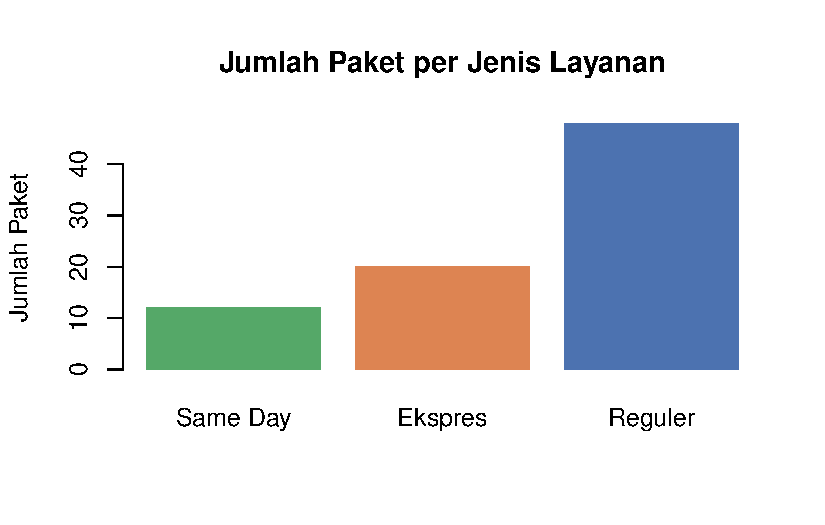
\includegraphics[keepaspectratio]{chapters/P04_files/figure-pdf/unnamed-chunk-27-1.pdf}}

\subsection{Langkah 2: Tabel Distribusi Frekuensi Waktu
Pengiriman}\label{langkah-2-tabel-distribusi-frekuensi-waktu-pengiriman}

\begin{Shaded}
\begin{Highlighting}[]
\NormalTok{n\_kirim }\OtherTok{\textless{}{-}} \FunctionTok{length}\NormalTok{(jam\_kirim)}
\NormalTok{k\_kirim }\OtherTok{\textless{}{-}} \FunctionTok{round}\NormalTok{(}\DecValTok{1} \SpecialCharTok{+} \FloatTok{3.322} \SpecialCharTok{*} \FunctionTok{log10}\NormalTok{(n\_kirim))}
\NormalTok{w\_kirim }\OtherTok{\textless{}{-}} \FunctionTok{ceiling}\NormalTok{((}\FunctionTok{max}\NormalTok{(jam\_kirim) }\SpecialCharTok{{-}} \FunctionTok{min}\NormalTok{(jam\_kirim)) }\SpecialCharTok{/}\NormalTok{ k\_kirim)}
\NormalTok{batas\_kirim }\OtherTok{\textless{}{-}} \FunctionTok{seq}\NormalTok{(}\FunctionTok{floor}\NormalTok{(}\FunctionTok{min}\NormalTok{(jam\_kirim)), }\AttributeTok{by =}\NormalTok{ w\_kirim, }\AttributeTok{length.out =}\NormalTok{ k\_kirim }\SpecialCharTok{+} \DecValTok{1}\NormalTok{)}
\FunctionTok{c}\NormalTok{(}\AttributeTok{k =}\NormalTok{ k\_kirim, }\AttributeTok{lebar =}\NormalTok{ w\_kirim)}
\end{Highlighting}
\end{Shaded}

\begin{verbatim}
    k lebar 
    7     9 
\end{verbatim}

\begin{Shaded}
\begin{Highlighting}[]
\NormalTok{f\_kirim }\OtherTok{\textless{}{-}} \FunctionTok{as.numeric}\NormalTok{(}\FunctionTok{table}\NormalTok{(}\FunctionTok{cut}\NormalTok{(jam\_kirim, }\AttributeTok{breaks =}\NormalTok{ batas\_kirim, }\AttributeTok{right =} \ConstantTok{FALSE}\NormalTok{)))}
\NormalTok{tabel\_kirim }\OtherTok{\textless{}{-}} \FunctionTok{data.frame}\NormalTok{(}
\AttributeTok{Interval\_jam =} \FunctionTok{paste0}\NormalTok{(}\StringTok{"["}\NormalTok{, }\FunctionTok{head}\NormalTok{(batas\_kirim, }\SpecialCharTok{{-}}\DecValTok{1}\NormalTok{), }\StringTok{", "}\NormalTok{, }\FunctionTok{tail}\NormalTok{(batas\_kirim, }\SpecialCharTok{{-}}\DecValTok{1}\NormalTok{), }\StringTok{")"}\NormalTok{),}
\AttributeTok{Titik\_Tengah =}\NormalTok{ (}\FunctionTok{head}\NormalTok{(batas\_kirim, }\SpecialCharTok{{-}}\DecValTok{1}\NormalTok{) }\SpecialCharTok{+} \FunctionTok{tail}\NormalTok{(batas\_kirim, }\SpecialCharTok{{-}}\DecValTok{1}\NormalTok{)) }\SpecialCharTok{/} \DecValTok{2}\NormalTok{,}
\AttributeTok{f =}\NormalTok{ f\_kirim,}
\AttributeTok{Persen =} \FunctionTok{round}\NormalTok{(f\_kirim }\SpecialCharTok{/}\NormalTok{ n\_kirim }\SpecialCharTok{*} \DecValTok{100}\NormalTok{, }\DecValTok{1}\NormalTok{),}
\AttributeTok{Persen\_Kum =} \FunctionTok{round}\NormalTok{(}\FunctionTok{cumsum}\NormalTok{(f\_kirim) }\SpecialCharTok{/}\NormalTok{ n\_kirim }\SpecialCharTok{*} \DecValTok{100}\NormalTok{, }\DecValTok{1}\NormalTok{)}
\NormalTok{)}
\NormalTok{knitr}\SpecialCharTok{::}\FunctionTok{kable}\NormalTok{(tabel\_kirim, }\AttributeTok{caption =} \StringTok{"Distribusi Frekuensi Waktu Pengiriman (jam)"}\NormalTok{)}
\end{Highlighting}
\end{Shaded}

\begin{longtable}[]{@{}lrrrr@{}}
\caption{Distribusi Frekuensi Waktu Pengiriman (jam)}\tabularnewline
\toprule\noalign{}
Interval\_jam & Titik\_Tengah & f & Persen & Persen\_Kum \\
\midrule\noalign{}
\endfirsthead
\toprule\noalign{}
Interval\_jam & Titik\_Tengah & f & Persen & Persen\_Kum \\
\midrule\noalign{}
\endhead
\bottomrule\noalign{}
\endlastfoot
{[}3, 12) & 7.5 & 12 & 15.0 & 15.0 \\
{[}12, 21) & 16.5 & 6 & 7.5 & 22.5 \\
{[}21, 30) & 25.5 & 14 & 17.5 & 40.0 \\
{[}30, 39) & 34.5 & 8 & 10.0 & 50.0 \\
{[}39, 48) & 43.5 & 18 & 22.5 & 72.5 \\
{[}48, 57) & 52.5 & 15 & 18.8 & 91.2 \\
{[}57, 66) & 61.5 & 7 & 8.8 & 100.0 \\
\end{longtable}

\begin{Shaded}
\begin{Highlighting}[]
\FunctionTok{sum}\NormalTok{(f\_kirim) }\SpecialCharTok{==}\NormalTok{ n\_kirim }\CommentTok{\# pastikan semua data tertampung}
\end{Highlighting}
\end{Shaded}

\begin{verbatim}
[1] TRUE
\end{verbatim}

Karena data kontinu dengan satu desimal, kita memakai interval setengah
terbuka \texttt{{[}a,\ b)} (\texttt{right\ =\ FALSE}), sehingga nilai
yang tepat berada di batas masuk ke kelas di atasnya.

\subsection{Langkah 3: Histogram dan
Ogive}\label{langkah-3-histogram-dan-ogive}

\begin{Shaded}
\begin{Highlighting}[]
\FunctionTok{par}\NormalTok{(}\AttributeTok{mfrow =} \FunctionTok{c}\NormalTok{(}\DecValTok{1}\NormalTok{, }\DecValTok{2}\NormalTok{))}
\FunctionTok{hist}\NormalTok{(jam\_kirim, }\AttributeTok{breaks =}\NormalTok{ batas\_kirim, }\AttributeTok{right =} \ConstantTok{FALSE}\NormalTok{, }\AttributeTok{col =} \StringTok{"\#4C72B0"}\NormalTok{, }\AttributeTok{border =} \StringTok{"white"}\NormalTok{,}
\AttributeTok{main =} \StringTok{"Histogram Waktu Pengiriman"}\NormalTok{, }\AttributeTok{xlab =} \StringTok{"Waktu pengiriman (jam)"}\NormalTok{, }\AttributeTok{ylab =} \StringTok{"Jumlah Paket"}\NormalTok{)}
\FunctionTok{plot}\NormalTok{(batas\_kirim, }\FunctionTok{c}\NormalTok{(}\DecValTok{0}\NormalTok{, }\FunctionTok{cumsum}\NormalTok{(f\_kirim)) }\SpecialCharTok{/}\NormalTok{ n\_kirim }\SpecialCharTok{*} \DecValTok{100}\NormalTok{, }\AttributeTok{type =} \StringTok{"b"}\NormalTok{, }\AttributeTok{pch =} \DecValTok{16}\NormalTok{, }\AttributeTok{lwd =} \DecValTok{2}\NormalTok{,}
\AttributeTok{col =} \StringTok{"\#DD8452"}\NormalTok{, }\AttributeTok{xlab =} \StringTok{"Waktu pengiriman (jam)"}\NormalTok{, }\AttributeTok{ylab =} \StringTok{"Persentase kumulatif (\%)"}\NormalTok{,}
\AttributeTok{main =} \StringTok{"Ogive Waktu Pengiriman"}\NormalTok{, }\AttributeTok{ylim =} \FunctionTok{c}\NormalTok{(}\DecValTok{0}\NormalTok{, }\DecValTok{100}\NormalTok{))}
\FunctionTok{abline}\NormalTok{(}\AttributeTok{h =} \FunctionTok{c}\NormalTok{(}\DecValTok{50}\NormalTok{, }\DecValTok{90}\NormalTok{), }\AttributeTok{lty =} \DecValTok{2}\NormalTok{, }\AttributeTok{col =} \StringTok{"grey50"}\NormalTok{)}
\end{Highlighting}
\end{Shaded}

\pandocbounded{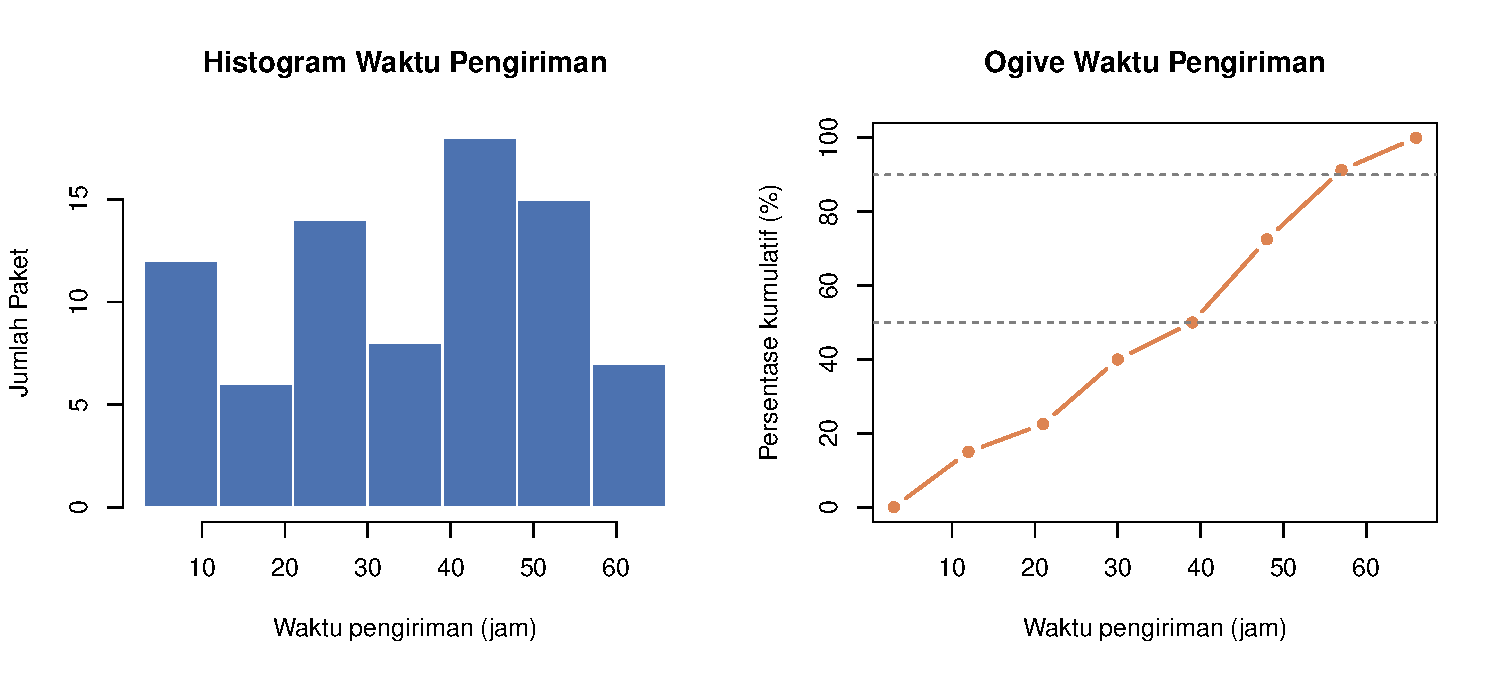
\includegraphics[keepaspectratio]{chapters/P04_files/figure-pdf/unnamed-chunk-31-1.pdf}}

\begin{Shaded}
\begin{Highlighting}[]
\FunctionTok{par}\NormalTok{(}\AttributeTok{mfrow =} \FunctionTok{c}\NormalTok{(}\DecValTok{1}\NormalTok{, }\DecValTok{1}\NormalTok{))}
\end{Highlighting}
\end{Shaded}

\subsection{Langkah 4: Histogram per
Layanan}\label{langkah-4-histogram-per-layanan}

\begin{Shaded}
\begin{Highlighting}[]
\FunctionTok{par}\NormalTok{(}\AttributeTok{mfrow =} \FunctionTok{c}\NormalTok{(}\DecValTok{1}\NormalTok{, }\DecValTok{3}\NormalTok{))}
\ControlFlowTok{for}\NormalTok{ (lay }\ControlFlowTok{in} \FunctionTok{c}\NormalTok{(}\StringTok{"Same Day"}\NormalTok{, }\StringTok{"Ekspres"}\NormalTok{, }\StringTok{"Reguler"}\NormalTok{)) \{}
\FunctionTok{hist}\NormalTok{(jam\_kirim[layanan }\SpecialCharTok{==}\NormalTok{ lay], }\AttributeTok{breaks =}\NormalTok{ batas\_kirim, }\AttributeTok{right =} \ConstantTok{FALSE}\NormalTok{,}
\AttributeTok{col =} \StringTok{"\#9ecae1"}\NormalTok{, }\AttributeTok{border =} \StringTok{"white"}\NormalTok{, }\AttributeTok{ylim =} \FunctionTok{c}\NormalTok{(}\DecValTok{0}\NormalTok{, }\DecValTok{25}\NormalTok{),}
\AttributeTok{main =}\NormalTok{ lay, }\AttributeTok{xlab =} \StringTok{"Waktu pengiriman (jam)"}\NormalTok{, }\AttributeTok{ylab =} \StringTok{"Jumlah Paket"}\NormalTok{)}
\NormalTok{\}}
\end{Highlighting}
\end{Shaded}

\pandocbounded{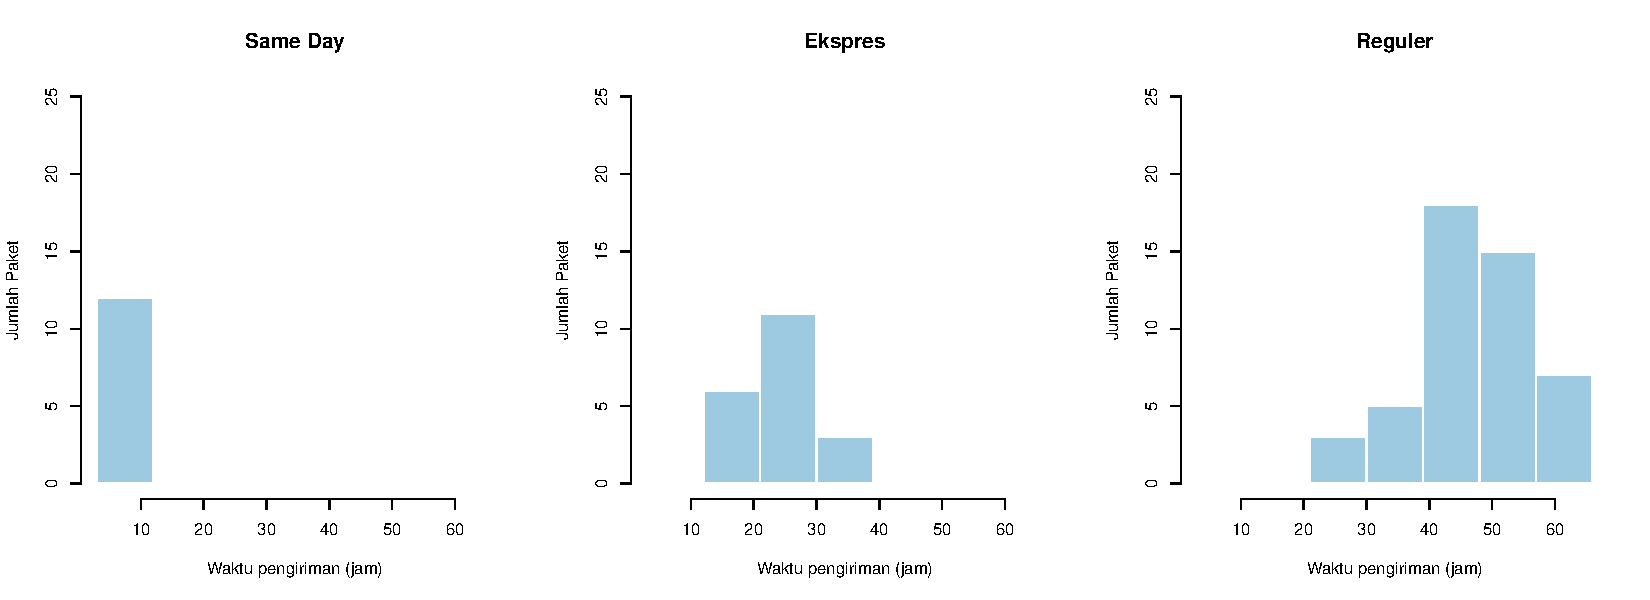
\includegraphics[keepaspectratio]{chapters/P04_files/figure-pdf/unnamed-chunk-32-1.pdf}}

\begin{Shaded}
\begin{Highlighting}[]
\FunctionTok{par}\NormalTok{(}\AttributeTok{mfrow =} \FunctionTok{c}\NormalTok{(}\DecValTok{1}\NormalTok{, }\DecValTok{1}\NormalTok{))}
\end{Highlighting}
\end{Shaded}

\subsection{Pertanyaan Diskusi dan
Jawaban}\label{pertanyaan-diskusi-dan-jawaban-3}

\textbf{1. Bagaimana bentuk distribusi waktu pengiriman secara
keseluruhan?}

Distribusinya \textbf{tidak satu puncak}: ada kelompok paket yang tiba
dalam hitungan jam, kelompok sekitar satu hari, dan kelompok terbesar
sekitar dua hari. Histogram per layanan menjelaskan penyebabnya -- data
sebenarnya campuran tiga layanan dengan waktu yang sangat berbeda.

\textbf{2. Mengapa melaporkan ``rata-rata waktu pengiriman'' saja tidak
tepat?}

Karena distribusinya campuran. Satu angka rata-rata (34.9 jam) tidak
mewakili pelanggan Same Day maupun Reguler. Laporan yang tepat
memisahkan distribusi per layanan.

\textbf{3. Informasi apa yang dapat dibaca dari ogive?}

Persentase paket yang tiba kurang dari 24 jam dapat dibaca dari ogive
dengan interpolasi linear: sekitar 28.3\% paket. Garis 90\% menunjukkan
batas waktu yang dipenuhi oleh 90\% pengiriman -- berguna untuk
menetapkan janji layanan (SLA).

\textbf{4. Grafik apa yang paling tepat untuk rapat manajemen?}

Diagram batang komposisi layanan (kategorik) dan histogram per layanan
(numerik), masing-masing dengan judul, satuan, dan \(n\). Diagram
lingkaran boleh dipakai untuk komposisi karena hanya ada tiga kategori.

\section{Latihan Mandiri}\label{latihan-mandiri-3}

\subsection{Latihan Utama (Exercise 2.14): Kepemilikan Kartu
Kredit}\label{latihan-utama-exercise-2.14-kepemilikan-kartu-kredit}

\textbf{Konteks:} Sebuah sampel acak dari 80 orang dewasa ditanya
mengenai jumlah kartu kredit yang mereka miliki. Hasilnya disajikan
dalam tabel berikut (data ini dilanjutkan pada Pertemuan 5).

\begin{Shaded}
\begin{Highlighting}[]
\NormalTok{kelas\_kk }\OtherTok{\textless{}{-}} \FunctionTok{c}\NormalTok{(}\StringTok{"0 to 3"}\NormalTok{, }\StringTok{"4 to 7"}\NormalTok{, }\StringTok{"8 to 11"}\NormalTok{, }\StringTok{"12 or more"}\NormalTok{)}
\NormalTok{frekuensi\_kk }\OtherTok{\textless{}{-}} \FunctionTok{c}\NormalTok{(}\DecValTok{18}\NormalTok{, }\DecValTok{26}\NormalTok{, }\DecValTok{22}\NormalTok{, }\DecValTok{14}\NormalTok{)}
\NormalTok{n\_kk }\OtherTok{\textless{}{-}} \FunctionTok{sum}\NormalTok{(frekuensi\_kk)}
\end{Highlighting}
\end{Shaded}

\subsubsection{Tugas 1: Lengkapi tabel dengan frekuensi relatif,
persentase, dan frekuensi
kumulatif}\label{tugas-1-lengkapi-tabel-dengan-frekuensi-relatif-persentase-dan-frekuensi-kumulatif}

\begin{Shaded}
\begin{Highlighting}[]
\NormalTok{tabel\_kk }\OtherTok{\textless{}{-}} \FunctionTok{data.frame}\NormalTok{(}
\AttributeTok{Kelas =}\NormalTok{ kelas\_kk,}
\AttributeTok{f =}\NormalTok{ frekuensi\_kk,}
\AttributeTok{f\_Relatif =}\NormalTok{ frekuensi\_kk }\SpecialCharTok{/}\NormalTok{ n\_kk,}
\AttributeTok{Persen =}\NormalTok{ frekuensi\_kk }\SpecialCharTok{/}\NormalTok{ n\_kk }\SpecialCharTok{*} \DecValTok{100}\NormalTok{,}
\AttributeTok{F\_Kumulatif =} \FunctionTok{cumsum}\NormalTok{(frekuensi\_kk),}
\AttributeTok{Persen\_Kum =} \FunctionTok{cumsum}\NormalTok{(frekuensi\_kk) }\SpecialCharTok{/}\NormalTok{ n\_kk }\SpecialCharTok{*} \DecValTok{100}
\NormalTok{)}
\NormalTok{knitr}\SpecialCharTok{::}\FunctionTok{kable}\NormalTok{(tabel\_kk, }\AttributeTok{digits =} \DecValTok{3}\NormalTok{, }\AttributeTok{caption =} \StringTok{"Distribusi Kepemilikan Kartu Kredit (n = 80)"}\NormalTok{)}
\end{Highlighting}
\end{Shaded}

\begin{longtable}[]{@{}lrrrrr@{}}
\caption{Distribusi Kepemilikan Kartu Kredit (n = 80)}\tabularnewline
\toprule\noalign{}
Kelas & f & f\_Relatif & Persen & F\_Kumulatif & Persen\_Kum \\
\midrule\noalign{}
\endfirsthead
\toprule\noalign{}
Kelas & f & f\_Relatif & Persen & F\_Kumulatif & Persen\_Kum \\
\midrule\noalign{}
\endhead
\bottomrule\noalign{}
\endlastfoot
0 to 3 & 18 & 0.225 & 22.5 & 18 & 22.5 \\
4 to 7 & 26 & 0.325 & 32.5 & 44 & 55.0 \\
8 to 11 & 22 & 0.275 & 27.5 & 66 & 82.5 \\
12 or more & 14 & 0.175 & 17.5 & 80 & 100.0 \\
\end{longtable}

\subsubsection{Tugas 2: Berapa persen responden yang memiliki 8 kartu
atau
lebih?}\label{tugas-2-berapa-persen-responden-yang-memiliki-8-kartu-atau-lebih}

\begin{Shaded}
\begin{Highlighting}[]
\FunctionTok{sum}\NormalTok{(frekuensi\_kk[}\DecValTok{3}\SpecialCharTok{:}\DecValTok{4}\NormalTok{]) }\SpecialCharTok{/}\NormalTok{ n\_kk }\SpecialCharTok{*} \DecValTok{100}
\end{Highlighting}
\end{Shaded}

\begin{verbatim}
[1] 45
\end{verbatim}

\textbf{Jawaban:} 45\% responden (22 + 14 = 36 orang) memiliki 8 kartu
kredit atau lebih.

\subsubsection{Tugas 3: Tentukan batas nyata dan titik tengah
kelas}\label{tugas-3-tentukan-batas-nyata-dan-titik-tengah-kelas}

\begin{Shaded}
\begin{Highlighting}[]
\NormalTok{batas\_nyata\_kk }\OtherTok{\textless{}{-}} \FunctionTok{c}\NormalTok{(}\SpecialCharTok{{-}}\FloatTok{0.5}\NormalTok{, }\FloatTok{3.5}\NormalTok{, }\FloatTok{7.5}\NormalTok{, }\FloatTok{11.5}\NormalTok{, }\FloatTok{15.5}\NormalTok{) }\CommentTok{\# kelas terbuka diasumsikan lebar 4}
\FunctionTok{data.frame}\NormalTok{(}\AttributeTok{Kelas =}\NormalTok{ kelas\_kk,}
\AttributeTok{Batas\_Nyata =} \FunctionTok{paste0}\NormalTok{(}\FunctionTok{head}\NormalTok{(batas\_nyata\_kk, }\SpecialCharTok{{-}}\DecValTok{1}\NormalTok{), }\StringTok{" {-} "}\NormalTok{, }\FunctionTok{tail}\NormalTok{(batas\_nyata\_kk, }\SpecialCharTok{{-}}\DecValTok{1}\NormalTok{)),}
\AttributeTok{Titik\_Tengah =}\NormalTok{ (}\FunctionTok{head}\NormalTok{(batas\_nyata\_kk, }\SpecialCharTok{{-}}\DecValTok{1}\NormalTok{) }\SpecialCharTok{+} \FunctionTok{tail}\NormalTok{(batas\_nyata\_kk, }\SpecialCharTok{{-}}\DecValTok{1}\NormalTok{)) }\SpecialCharTok{/} \DecValTok{2}\NormalTok{)}
\end{Highlighting}
\end{Shaded}

\begin{verbatim}
       Kelas Batas_Nyata Titik_Tengah
1     0 to 3  -0.5 - 3.5          1.5
2     4 to 7   3.5 - 7.5          5.5
3    8 to 11  7.5 - 11.5          9.5
4 12 or more 11.5 - 15.5         13.5
\end{verbatim}

\textbf{Catatan:} kelas ``12 or more'' adalah \textbf{kelas terbuka}
(tidak punya batas atas). Untuk menggambar histogram atau menghitung
titik tengah, kita harus berasumsi -- di sini lebarnya disamakan dengan
kelas lain (12--15). Asumsi ini \textbf{wajib dinyatakan}.

\subsubsection{Tugas 4: Gambar histogram dan poligon
frekuensinya}\label{tugas-4-gambar-histogram-dan-poligon-frekuensinya}

\begin{Shaded}
\begin{Highlighting}[]
\NormalTok{m\_kk }\OtherTok{\textless{}{-}}\NormalTok{ (}\FunctionTok{head}\NormalTok{(batas\_nyata\_kk, }\SpecialCharTok{{-}}\DecValTok{1}\NormalTok{) }\SpecialCharTok{+} \FunctionTok{tail}\NormalTok{(batas\_nyata\_kk, }\SpecialCharTok{{-}}\DecValTok{1}\NormalTok{)) }\SpecialCharTok{/} \DecValTok{2}
\FunctionTok{plot}\NormalTok{(}\ConstantTok{NULL}\NormalTok{, }\AttributeTok{xlim =} \FunctionTok{c}\NormalTok{(}\SpecialCharTok{{-}}\FloatTok{4.5}\NormalTok{, }\FloatTok{19.5}\NormalTok{), }\AttributeTok{ylim =} \FunctionTok{c}\NormalTok{(}\DecValTok{0}\NormalTok{, }\DecValTok{30}\NormalTok{), }\AttributeTok{xaxt =} \StringTok{"n"}\NormalTok{,}
\AttributeTok{xlab =} \StringTok{"Jumlah Kartu Kredit"}\NormalTok{, }\AttributeTok{ylab =} \StringTok{"Frekuensi (f)"}\NormalTok{,}
\AttributeTok{main =} \StringTok{"Distribusi Kepemilikan Kartu Kredit (n = 80)"}\NormalTok{)}
\FunctionTok{rect}\NormalTok{(}\FunctionTok{head}\NormalTok{(batas\_nyata\_kk, }\SpecialCharTok{{-}}\DecValTok{1}\NormalTok{), }\DecValTok{0}\NormalTok{, }\FunctionTok{tail}\NormalTok{(batas\_nyata\_kk, }\SpecialCharTok{{-}}\DecValTok{1}\NormalTok{), frekuensi\_kk,}
\AttributeTok{col =} \StringTok{"\#6C5B7B"}\NormalTok{, }\AttributeTok{border =} \StringTok{"white"}\NormalTok{)}
\FunctionTok{lines}\NormalTok{(}\FunctionTok{c}\NormalTok{(}\SpecialCharTok{{-}}\FloatTok{2.5}\NormalTok{, m\_kk, }\FloatTok{17.5}\NormalTok{), }\FunctionTok{c}\NormalTok{(}\DecValTok{0}\NormalTok{, frekuensi\_kk, }\DecValTok{0}\NormalTok{), }\AttributeTok{type =} \StringTok{"b"}\NormalTok{, }\AttributeTok{pch =} \DecValTok{16}\NormalTok{, }\AttributeTok{col =} \StringTok{"\#F8B195"}\NormalTok{, }\AttributeTok{lwd =} \DecValTok{2}\NormalTok{)}
\FunctionTok{axis}\NormalTok{(}\DecValTok{1}\NormalTok{, }\AttributeTok{at =}\NormalTok{ batas\_nyata\_kk)}
\FunctionTok{text}\NormalTok{(m\_kk, frekuensi\_kk, frekuensi\_kk, }\AttributeTok{pos =} \DecValTok{3}\NormalTok{)}
\end{Highlighting}
\end{Shaded}

\pandocbounded{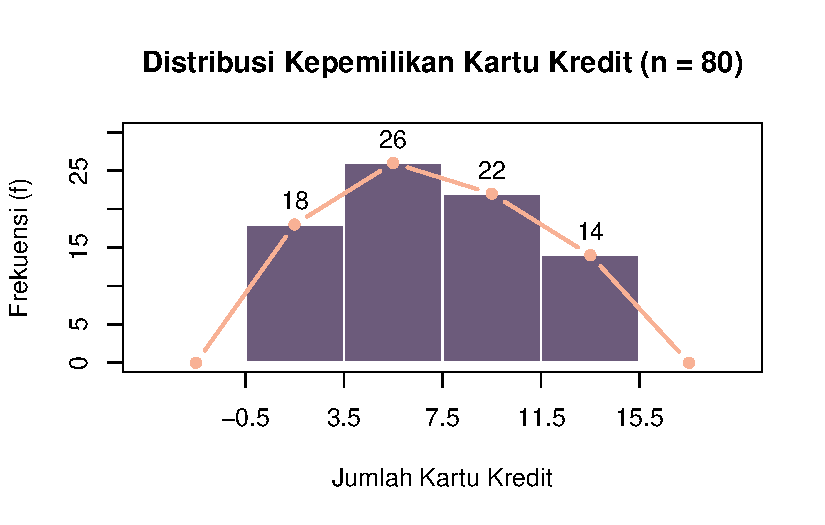
\includegraphics[keepaspectratio]{chapters/P04_files/figure-pdf/unnamed-chunk-37-1.pdf}}

\subsubsection{Tugas 5: Interpretasikan
distribusinya}\label{tugas-5-interpretasikan-distribusinya}

\textbf{Jawaban:} Kelas dengan frekuensi terbanyak adalah \textbf{4 to
7} (26 orang, 32,5\%). Frekuensi naik dari kelas pertama ke kelas kedua
lalu turun perlahan, sehingga distribusinya \textbf{sedikit menjulur ke
kanan}. Sebanyak 44 responden (55\%, dari frekuensi kumulatif kelas
kedua) memiliki 7 kartu atau kurang. Ukuran pusat dan sebarannya
dihitung pada Pertemuan 5.

\subsubsection{Tugas 6 (Tantangan): Diagram batang atau
histogram?}\label{tugas-6-tantangan-diagram-batang-atau-histogram}

Jumlah kartu kredit adalah data \textbf{diskrit}. Apakah lebih tepat
digambarkan dengan diagram batang atau histogram? Jelaskan.

\textbf{Jawaban:} Jika data mentah tersedia dengan sedikit nilai berbeda
(misalnya 0--15), diagram batang per nilai paling informatif. Namun
karena data sudah dikelompokkan menjadi interval bersambung (0--3, 4--7,
\ldots), histogram dengan batas nyata tepat dipakai -- batasnya menempel
karena setiap bilangan bulat pasti masuk satu kelas. Yang penting: kelas
terbuka ``12 or more'' diberi catatan asumsi.

\subsection{Latihan Tambahan
(Self-Check)}\label{latihan-tambahan-self-check-3}

Kerjakan soal-soal berikut secara mandiri sebelum melihat kunci jawaban
pada komentar kode.

\textbf{Soal A.} Data usia (tahun) 25 peserta pelatihan: 23, 31, 27, 45,
38, 29, 34, 41, 26, 36, 52, 30, 28, 33, 47, 39, 24, 35, 43, 32, 37, 29,
48, 31, 40. Susun tabel distribusi frekuensi dengan Aturan Sturges,
lengkap dengan batas nyata, titik tengah, frekuensi relatif, dan
kumulatif.

\begin{Shaded}
\begin{Highlighting}[]
\NormalTok{usia }\OtherTok{\textless{}{-}} \FunctionTok{c}\NormalTok{(}\DecValTok{23}\NormalTok{, }\DecValTok{31}\NormalTok{, }\DecValTok{27}\NormalTok{, }\DecValTok{45}\NormalTok{, }\DecValTok{38}\NormalTok{, }\DecValTok{29}\NormalTok{, }\DecValTok{34}\NormalTok{, }\DecValTok{41}\NormalTok{, }\DecValTok{26}\NormalTok{, }\DecValTok{36}\NormalTok{, }\DecValTok{52}\NormalTok{, }\DecValTok{30}\NormalTok{, }\DecValTok{28}\NormalTok{, }\DecValTok{33}\NormalTok{, }\DecValTok{47}\NormalTok{, }\DecValTok{39}\NormalTok{, }\DecValTok{24}\NormalTok{, }\DecValTok{35}\NormalTok{, }\DecValTok{43}\NormalTok{,}
\DecValTok{32}\NormalTok{, }\DecValTok{37}\NormalTok{, }\DecValTok{29}\NormalTok{, }\DecValTok{48}\NormalTok{, }\DecValTok{31}\NormalTok{, }\DecValTok{40}\NormalTok{)}
\CommentTok{\# Kunci jawaban:}
\CommentTok{\# k = 1 + 3.322 log10(25) = 5.64 {-}\textgreater{} 6 kelas; R = 52 {-} 23 = 29; w = 29/6 = 4.83 {-}\textgreater{} 5}
\CommentTok{\# Kelas: 23{-}27, 28{-}32, 33{-}37, 38{-}42, 43{-}47, 48{-}52}
\CommentTok{\# Batas nyata: 22.5, 27.5, 32.5, 37.5, 42.5, 47.5, 52.5}
\FunctionTok{table}\NormalTok{(}\FunctionTok{cut}\NormalTok{(usia, }\AttributeTok{breaks =} \FunctionTok{seq}\NormalTok{(}\FloatTok{22.5}\NormalTok{, }\FloatTok{52.5}\NormalTok{, }\AttributeTok{by =} \DecValTok{5}\NormalTok{)))}
\end{Highlighting}
\end{Shaded}

\begin{verbatim}

(22.5,27.5] (27.5,32.5] (32.5,37.5] (37.5,42.5] (42.5,47.5] (47.5,52.5] 
          4           7           5           4           3           2 
\end{verbatim}

\begin{Shaded}
\begin{Highlighting}[]
\CommentTok{\# f = 4, 7, 5, 4, 3, 2 (total 25); titik tengah = 25, 30, 35, 40, 45, 50}
\end{Highlighting}
\end{Shaded}

\textbf{Soal B.} Buat diagram batang-daun untuk data usia pada Soal A,
lalu tentukan usia yang paling sering muncul.

\begin{Shaded}
\begin{Highlighting}[]
\FunctionTok{stem}\NormalTok{(usia)}
\end{Highlighting}
\end{Shaded}

\begin{verbatim}

  The decimal point is 1 digit(s) to the right of the |

  2 | 3467899
  3 | 01123456789
  4 | 013578
  5 | 2
\end{verbatim}

\begin{Shaded}
\begin{Highlighting}[]
\CommentTok{\# Kunci jawaban: batang 2, 3, 4, 5. Usia 29 dan 31 masing{-}masing muncul dua kali}
\CommentTok{\# (terlihat sebagai daun "99" pada batang 2 dan "11" pada batang 3).}
\end{Highlighting}
\end{Shaded}

\textbf{Soal C.} Sebuah media menampilkan diagram batang penjualan dua
merek dengan sumbu-y dari 950 sampai 1.000 unit (Merek A = 960, Merek B
= 990). Jelaskan mengapa grafik itu menyesatkan dan hitung perbandingan
panjang batang yang tampak vs yang seharusnya.

\begin{Shaded}
\begin{Highlighting}[]
\CommentTok{\# Kunci jawaban:}
\NormalTok{(}\DecValTok{990} \SpecialCharTok{{-}} \DecValTok{950}\NormalTok{) }\SpecialCharTok{/}\NormalTok{ (}\DecValTok{960} \SpecialCharTok{{-}} \DecValTok{950}\NormalTok{) }\CommentTok{\# tampak: batang B = 4 kali batang A}
\end{Highlighting}
\end{Shaded}

\begin{verbatim}
[1] 4
\end{verbatim}

\begin{Shaded}
\begin{Highlighting}[]
\DecValTok{990} \SpecialCharTok{/} \DecValTok{960} \CommentTok{\# seharusnya: B hanya \textasciitilde{}1.03 kali A (lebih besar 3\%)}
\end{Highlighting}
\end{Shaded}

\begin{verbatim}
[1] 1.03125
\end{verbatim}

\begin{Shaded}
\begin{Highlighting}[]
\CommentTok{\# Diagram batang harus dimulai dari 0 agar panjang batang sebanding dengan nilainya.}
\end{Highlighting}
\end{Shaded}

\textbf{Soal D.} Dari tabel pendapatan mingguan pada praktikum ini,
berapa persen karyawan yang berpendapatan lebih dari 1.600,5 USD? Kelas
mana yang memuat median?

\begin{Shaded}
\begin{Highlighting}[]
\CommentTok{\# Kunci jawaban:}
\FunctionTok{sum}\NormalTok{(f\_p[}\DecValTok{5}\SpecialCharTok{:}\DecValTok{6}\NormalTok{]) }\SpecialCharTok{/} \FunctionTok{sum}\NormalTok{(f\_p) }\SpecialCharTok{*} \DecValTok{100} \CommentTok{\# (9 + 6) / 100 = 15\%}
\end{Highlighting}
\end{Shaded}

\begin{verbatim}
[1] 15
\end{verbatim}

\begin{Shaded}
\begin{Highlighting}[]
\FunctionTok{cumsum}\NormalTok{(f\_p) }\CommentTok{\# 9, 31, 70, ... {-}\textgreater{} posisi median ke{-}50 berada di kelas 1201{-}1400}
\end{Highlighting}
\end{Shaded}

\begin{verbatim}
[1]   9  31  70  85  94 100
\end{verbatim}

\section{Kesalahan Umum dalam Penyajian dan Visualisasi
Data}\label{kesalahan-umum-dalam-penyajian-dan-visualisasi-data}

\begin{enumerate}
\def\labelenumi{\arabic{enumi}.}
\tightlist
\item
  Memakai \textbf{histogram untuk data kategorik} (atau diagram batang
  dengan batang menempel untuk kategori) -- pilih grafik sesuai jenis
  data.
\item
  \textbf{Memotong sumbu-y} diagram batang -- perbedaan kecil tampak
  sangat besar.
\item
  Diagram lingkaran dengan \textbf{terlalu banyak irisan} atau total
  yang bukan 100\%.
\item
  Grafik \textbf{tanpa judul, label sumbu, satuan, atau} \(n\) --
  pembaca tidak dapat menafsirkan.
\item
  Memilih \textbf{banyak kelas asal-asalan} -- terlalu sedikit
  menyembunyikan pola, terlalu banyak menimbulkan pola palsu.
\item
  \textbf{Lebar kelas dibulatkan ke bawah} sehingga data terbesar tidak
  tertampung -- lebar kelas dibulatkan \textbf{ke atas}.
\item
  \textbf{Kelas yang tumpang tindih atau berlubang} (misalnya 60--70 dan
  70--80) -- satu nilai tidak boleh masuk dua kelas; gunakan batas nyata
  atau interval setengah terbuka yang konsisten.
\item
  Menghitung \textbf{frekuensi kumulatif untuk data nominal} tanpa
  urutan yang bermakna.
\item
  \textbf{Tidak menyatakan asumsi kelas terbuka} (``12 or more'') saat
  menggambar histogram atau menghitung titik tengah.
\item
  \textbf{Mengurutkan kategori ordinal menurut abjad} -- urutan harus
  mengikuti tingkatannya.
\item
  \textbf{Membandingkan persentase tabel silang ke arah yang salah} --
  pilih persentase baris atau kolom sesuai pertanyaan.
\item
  \textbf{Efek 3D dan dekorasi berlebihan} yang mendistorsi proporsi.
\end{enumerate}

\section{Cheat Sheet: Fungsi R yang
Digunakan}\label{cheat-sheet-fungsi-r-yang-digunakan-3}

{\def\LTcaptype{none} % do not increment counter
\begin{longtable}[]{@{}
  >{\raggedright\arraybackslash}p{(\linewidth - 2\tabcolsep) * \real{0.5000}}
  >{\raggedright\arraybackslash}p{(\linewidth - 2\tabcolsep) * \real{0.5000}}@{}}
\toprule\noalign{}
\begin{minipage}[b]{\linewidth}\raggedright
Fungsi
\end{minipage} & \begin{minipage}[b]{\linewidth}\raggedright
Kegunaan
\end{minipage} \\
\midrule\noalign{}
\endhead
\bottomrule\noalign{}
\endlastfoot
\texttt{table(x)} & Frekuensi tiap kategori/nilai \\
\texttt{prop.table(tabel,\ margin)} & Frekuensi relatif;
\texttt{margin\ =\ 1} per baris, \texttt{2} per kolom \\
\texttt{addmargins(tabel)} & Menambahkan total baris dan kolom \\
\texttt{sort(tabel,\ decreasing\ =\ TRUE)} & Mengurutkan frekuensi
(untuk Pareto) \\
\texttt{cumsum(f)} & Frekuensi kumulatif \\
\texttt{rev(cumsum(rev(f)))} & Frekuensi kumulatif ``lebih dari'' \\
\texttt{log10(n)}, \texttt{ceiling(x)}, \texttt{round(x)} & Perhitungan
Aturan Sturges dan lebar kelas \\
\texttt{nclass.Sturges(x)}, \texttt{nclass.FD(x)},
\texttt{nclass.scott(x)} & Banyak kelas menurut berbagai aturan \\
\texttt{seq(from,\ by,\ length.out)} & Membuat batas kelas \\
\texttt{cut(x,\ breaks,\ right\ =\ TRUE/FALSE)} & Mengelompokkan data ke
kelas \\
\texttt{hist(x,\ breaks,\ plot\ =\ FALSE)} & Menghitung frekuensi kelas
tanpa menggambar \\
\texttt{barplot(f,\ horiz,\ beside)} & Diagram batang (horizontal,
berkelompok, bertumpuk) \\
\texttt{pie(f,\ labels)} & Diagram lingkaran \\
\texttt{hist(x,\ breaks)} & Histogram \\
\texttt{rect(x1,\ y1,\ x2,\ y2)} & Menggambar histogram dari data
terkelompok \\
\texttt{lines(x,\ y,\ type\ =\ "b")} & Poligon frekuensi / ogive / garis
kumulatif Pareto \\
\texttt{approx(x,\ y,\ xout)} & Interpolasi linear (menaksir median dari
ogive) \\
\texttt{stem(x,\ scale)} & Diagram batang-daun \\
\texttt{axis()}, \texttt{text()}, \texttt{legend()}, \texttt{abline()} &
Melengkapi grafik dengan sumbu, label, legenda, garis bantu \\
\texttt{par(mfrow\ =\ c(r,\ c))}, \texttt{par(mar\ =\ ...)} & Mengatur
tata letak dan margin grafik \\
\end{longtable}
}

\section{Glosarium Istilah}\label{glosarium-istilah-3}

{\def\LTcaptype{none} % do not increment counter
\begin{longtable}[]{@{}
  >{\raggedright\arraybackslash}p{(\linewidth - 2\tabcolsep) * \real{0.5000}}
  >{\raggedright\arraybackslash}p{(\linewidth - 2\tabcolsep) * \real{0.5000}}@{}}
\toprule\noalign{}
\begin{minipage}[b]{\linewidth}\raggedright
Istilah
\end{minipage} & \begin{minipage}[b]{\linewidth}\raggedright
Definisi Singkat
\end{minipage} \\
\midrule\noalign{}
\endhead
\bottomrule\noalign{}
\endlastfoot
Distribusi Frekuensi & Tabel yang menunjukkan banyaknya data pada setiap
kategori atau kelas \\
Frekuensi Relatif & Frekuensi dibagi banyaknya data (\(f/n\)) \\
Frekuensi Kumulatif & Jumlah frekuensi hingga kelas tertentu \\
Tabel Silang & Tabel frekuensi dua variabel kategorik sekaligus \\
Aturan Sturges & Aturan menentukan banyak kelas:
\(k = 1 + 3,322 \log_{10} n\) \\
Lebar Kelas & Selisih batas nyata atas dan bawah sebuah kelas \\
Batas Kelas & Nilai terkecil dan terbesar yang tercantum pada sebuah
kelas \\
Batas Nyata & Batas kelas yang diperluas setengah satuan agar kelas
bersambung \\
Titik Tengah Kelas & Rata-rata batas bawah dan atas kelas; wakil nilai
kelas \\
Kelas Terbuka & Kelas tanpa batas bawah atau batas atas (misalnya ``12
or more'') \\
Diagram Batang & Grafik batang terpisah untuk frekuensi data
kategorik \\
Diagram Pareto & Diagram batang terurut dengan garis persentase
kumulatif \\
Diagram Lingkaran & Grafik irisan lingkaran yang menunjukkan bagian dari
keseluruhan \\
Histogram & Grafik batang bersambung untuk distribusi data numerik \\
Poligon Frekuensi & Garis yang menghubungkan titik tengah puncak kelas
histogram \\
Ogive & Kurva frekuensi kumulatif terhadap batas nyata atas \\
Stem-and-Leaf & Diagram yang memecah nilai menjadi batang dan daun
sambil mempertahankan nilai asli \\
Bin & Istilah lain untuk kelas/interval pada histogram \\
\end{longtable}
}

\section{Rangkuman dan Kesimpulan}\label{rangkuman-dan-kesimpulan-3}

\begin{enumerate}
\def\labelenumi{\arabic{enumi}.}
\tightlist
\item
  \textbf{Tabel distribusi frekuensi} meringkas data menjadi frekuensi,
  frekuensi relatif, dan frekuensi kumulatif. \textbf{Tabel silang}
  meringkas hubungan dua variabel kategorik.
\item
  Data numerik dikelompokkan dengan \textbf{Aturan Sturges}, lebar kelas
  yang \textbf{dibulatkan ke atas}, \textbf{batas nyata} agar kelas
  bersambung, dan \textbf{titik tengah} sebagai wakil kelas.
\item
  \textbf{Jenis data menentukan grafik}: diagram batang/lingkaran/Pareto
  untuk kategorik; histogram, poligon, ogive, dan stem-and-leaf untuk
  numerik.
\item
  \textbf{Visualisasi yang jujur} memulai sumbu diagram batang dari nol,
  memberi label lengkap, memilih bin dengan cermat, dan menghindari
  dekorasi yang mendistorsi.
\item
  Membaca grafik berarti menceritakan \textbf{bentuk, pusat, sebaran,
  dan keanehan} data.
\end{enumerate}

\textbf{Jembatan ke sesi berikutnya:} Pertemuan 5 mengubah kesan visual
``pusat di sekitar 80'' dan ``sebaran dari 63 sampai 95'' menjadi angka
yang tepat -- mean, median, modus, rentang, varians, simpangan baku, dan
koefisien variasi -- termasuk perhitungannya dari tabel data terkelompok
yang telah kita susun hari ini.

\section{Referensi Pendukung}\label{referensi-pendukung-3}

Materi ini merangkum topik penyajian data dan visualisasi
(\emph{organizing and visualizing data}) yang umum dibahas pada bab awal
buku teks pengantar statistika bisnis/data science. Mahasiswa disarankan
melengkapi pemahaman dengan merujuk pada:

\begin{itemize}
\tightlist
\item
  Modul/slide perkuliahan ``Introduction to Statistics (SDT-1102)'' --
  Pertemuan 4: Penyajian dan Visualisasi Data.
\item
  Tufte, E. R. \emph{The Visual Display of Quantitative Information}.
  Graphics Press.
\item
  Huff, D. \emph{How to Lie with Statistics}. W. W. Norton (bab tentang
  grafik yang menyesatkan).
\item
  Dokumentasi resmi R: \texttt{?table}, \texttt{?cut}, \texttt{?hist},
  \texttt{?barplot}, \texttt{?pie}, \texttt{?stem},
  \texttt{?nclass.Sturges} (dapat diakses langsung di R/RStudio).
\end{itemize}

\bookmarksetup{startatroot}

\chapter{Ukuran Pemusatan dan Penyebaran
Data}\label{ukuran-pemusatan-dan-penyebaran-data}

\section{Prasyarat dan Notasi}\label{prasyarat-dan-notasi}

\subsection{Skala Pengukuran Menentukan Ukuran yang
Valid}\label{skala-pengukuran-menentukan-ukuran-yang-valid}

Ingat kembali skala pengukuran dari Pertemuan 2. Skala data menentukan
ukuran mana yang bermakna untuk dihitung:

{\def\LTcaptype{none} % do not increment counter
\begin{longtable}[]{@{}lllll@{}}
\toprule\noalign{}
Skala & Modus & Median & Mean & Ukuran Penyebaran \\
\midrule\noalign{}
\endhead
\bottomrule\noalign{}
\endlastfoot
Nominal & Ya & Tidak & Tidak & Tidak berlaku \\
Ordinal & Ya & Ya & Kurang tepat & Kuartil / IQR \\
Interval & Ya & Ya & Ya & Rentang, IQR, varians, simpangan baku \\
Rasio & Ya & Ya & Ya & Semua ukuran, termasuk koefisien variasi \\
\end{longtable}
}

Contoh: ``rata-rata golongan darah'' tidak bermakna (nominal), sedangkan
``rata-rata tinggi badan'' bermakna (rasio).

\subsection{Populasi vs Sampel: Notasi}\label{populasi-vs-sampel-notasi}

Karena statistik dari \textbf{sampel} dipakai untuk menduga parameter
\textbf{populasi}, notasinya dibedakan:

{\def\LTcaptype{none} % do not increment counter
\begin{longtable}[]{@{}lll@{}}
\toprule\noalign{}
Ukuran & Populasi (Parameter) & Sampel (Statistik) \\
\midrule\noalign{}
\endhead
\bottomrule\noalign{}
\endlastfoot
Banyaknya data & \(N\) & \(n\) \\
Rata-rata & \(\mu\) & \(\bar{x}\) \\
Varians & \(\sigma^2\) & \(s^2\) \\
Simpangan baku & \(\sigma\) & \(s\) \\
\end{longtable}
}

Simbol \(\sum\) (sigma besar) berarti ``jumlahkan'':
\(\sum_{i=1}^{n} x_i = x_1 + x_2 + \cdots + x_n\).

\subsection{Data Utama yang Dipakai}\label{data-utama-yang-dipakai}

Sepanjang praktikum, kita memakai nilai ujian Statistika 30 mahasiswa
dari Pertemuan 4. Pengelompokan kelasnya (Aturan Sturges: 6 kelas, lebar
6, batas nyata dimulai dari 62,5) sudah kita peroleh dan dipakai ulang
pada bagian data terkelompok.

\begin{Shaded}
\begin{Highlighting}[]
\NormalTok{nilai\_ujian }\OtherTok{\textless{}{-}} \FunctionTok{c}\NormalTok{(}\DecValTok{78}\NormalTok{, }\DecValTok{65}\NormalTok{, }\DecValTok{82}\NormalTok{, }\DecValTok{90}\NormalTok{, }\DecValTok{74}\NormalTok{, }\DecValTok{68}\NormalTok{, }\DecValTok{95}\NormalTok{, }\DecValTok{88}\NormalTok{, }\DecValTok{72}\NormalTok{, }\DecValTok{80}\NormalTok{,}
\DecValTok{91}\NormalTok{, }\DecValTok{77}\NormalTok{, }\DecValTok{63}\NormalTok{, }\DecValTok{85}\NormalTok{, }\DecValTok{79}\NormalTok{, }\DecValTok{92}\NormalTok{, }\DecValTok{70}\NormalTok{, }\DecValTok{84}\NormalTok{, }\DecValTok{76}\NormalTok{, }\DecValTok{89}\NormalTok{,}
\DecValTok{81}\NormalTok{, }\DecValTok{67}\NormalTok{, }\DecValTok{93}\NormalTok{, }\DecValTok{75}\NormalTok{, }\DecValTok{86}\NormalTok{, }\DecValTok{71}\NormalTok{, }\DecValTok{94}\NormalTok{, }\DecValTok{83}\NormalTok{, }\DecValTok{69}\NormalTok{, }\DecValTok{87}\NormalTok{)}
\NormalTok{n }\OtherTok{\textless{}{-}} \FunctionTok{length}\NormalTok{(nilai\_ujian)}
\CommentTok{\# Batas nyata kelas hasil pengelompokan pada Pertemuan 4}
\NormalTok{batas\_nyata\_u }\OtherTok{\textless{}{-}} \FunctionTok{seq}\NormalTok{(}\FloatTok{62.5}\NormalTok{, }\AttributeTok{by =} \DecValTok{6}\NormalTok{, }\AttributeTok{length.out =} \DecValTok{7}\NormalTok{)}
\end{Highlighting}
\end{Shaded}

\begin{Shaded}
\begin{Highlighting}[]
\NormalTok{f\_ujian }\OtherTok{\textless{}{-}} \FunctionTok{as.numeric}\NormalTok{(}\FunctionTok{table}\NormalTok{(}\FunctionTok{cut}\NormalTok{(nilai\_ujian, }\AttributeTok{breaks =}\NormalTok{ batas\_nyata\_u)))}
\NormalTok{n}
\end{Highlighting}
\end{Shaded}

\begin{verbatim}
[1] 30
\end{verbatim}

\begin{Shaded}
\begin{Highlighting}[]
\FunctionTok{sort}\NormalTok{(nilai\_ujian)}
\end{Highlighting}
\end{Shaded}

\begin{verbatim}
 [1] 63 65 67 68 69 70 71 72 74 75 76 77 78 79 80 81 82 83 84 85 86 87 88 89 90
[26] 91 92 93 94 95
\end{verbatim}

\begin{Shaded}
\begin{Highlighting}[]
\FunctionTok{hist}\NormalTok{(nilai\_ujian, }\AttributeTok{breaks =}\NormalTok{ batas\_nyata\_u, }\AttributeTok{col =} \StringTok{"\#4C72B0"}\NormalTok{, }\AttributeTok{border =} \StringTok{"white"}\NormalTok{,}
\AttributeTok{main =} \StringTok{"Nilai Ujian Statistika (n = 30)"}\NormalTok{, }\AttributeTok{xlab =} \StringTok{"Nilai Ujian"}\NormalTok{, }\AttributeTok{ylab =} \StringTok{"Frekuensi"}\NormalTok{)}
\end{Highlighting}
\end{Shaded}

\pandocbounded{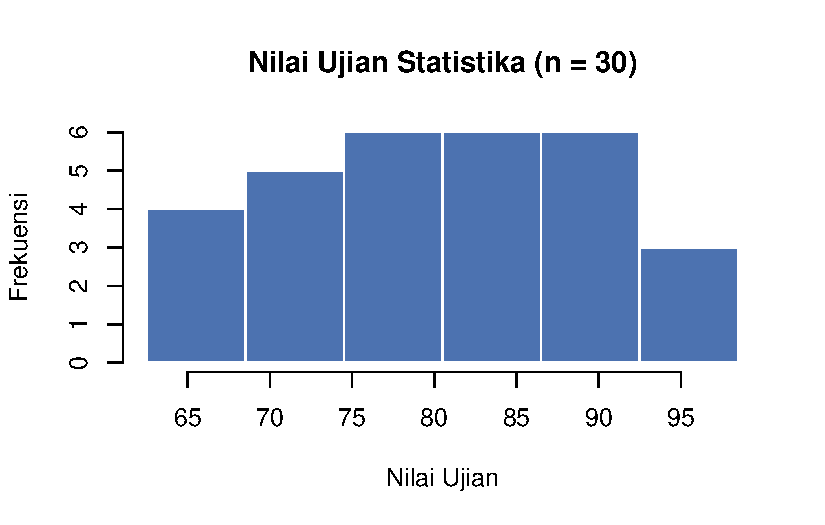
\includegraphics[keepaspectratio]{chapters/P05_files/figure-pdf/unnamed-chunk-3-1.pdf}}

Dari histogram, kita bisa memperkirakan ``pusat'' data ada di sekitar 80
dan sebarannya kira-kira dari 63 sampai 95. Praktikum ini mengubah
\textbf{perkiraan visual} tersebut menjadi \textbf{angka yang tepat}.

\section{Ukuran Pemusatan Data}\label{ukuran-pemusatan-data}

\subsection{Rata-rata Hitung (Mean)}\label{rata-rata-hitung-mean}

Mean adalah jumlah seluruh nilai dibagi banyaknya data:

\[\mu = \frac{\sum_{i=1}^{N} x_i}{N} \qquad\qquad \bar{x} = \frac{\sum_{i=1}^{n} x_i}{n}\]

\begin{Shaded}
\begin{Highlighting}[]
\CommentTok{\# Manual: jumlahkan lalu bagi n}
\FunctionTok{sum}\NormalTok{(nilai\_ujian) }\SpecialCharTok{/}\NormalTok{ n}
\end{Highlighting}
\end{Shaded}

\begin{verbatim}
[1] 80.13333
\end{verbatim}

\begin{Shaded}
\begin{Highlighting}[]
\CommentTok{\# Fungsi bawaan R}
\FunctionTok{mean}\NormalTok{(nilai\_ujian)}
\end{Highlighting}
\end{Shaded}

\begin{verbatim}
[1] 80.13333
\end{verbatim}

\textbf{Sifat penting mean:}

\begin{enumerate}
\def\labelenumi{\arabic{enumi}.}
\tightlist
\item
  Memakai \textbf{seluruh} nilai data.
\item
  Jumlah selisih (deviasi) semua data terhadap mean selalu \textbf{nol}:
  \(\sum (x_i - \bar{x}) = 0\). Karena itu mean disebut \textbf{titik
  keseimbangan} data.
\item
  \textbf{Sensitif terhadap outlier} -- satu nilai ekstrem dapat
  menggeser mean secara drastis.
\end{enumerate}

\begin{Shaded}
\begin{Highlighting}[]
\FunctionTok{round}\NormalTok{(}\FunctionTok{sum}\NormalTok{(nilai\_ujian }\SpecialCharTok{{-}} \FunctionTok{mean}\NormalTok{(nilai\_ujian)), }\DecValTok{10}\NormalTok{)   }\CommentTok{\# selalu 0}
\end{Highlighting}
\end{Shaded}

\begin{verbatim}
[1] 0
\end{verbatim}

\begin{Shaded}
\begin{Highlighting}[]
\FunctionTok{stripchart}\NormalTok{(nilai\_ujian, }\AttributeTok{method =} \StringTok{"jitter"}\NormalTok{, }\AttributeTok{pch =} \DecValTok{16}\NormalTok{, }\AttributeTok{col =} \StringTok{"steelblue"}\NormalTok{,}
\AttributeTok{xlab =} \StringTok{"Nilai Ujian"}\NormalTok{, }\AttributeTok{main =} \StringTok{"Mean sebagai Titik Keseimbangan"}\NormalTok{)}
\FunctionTok{abline}\NormalTok{(}\AttributeTok{v =} \FunctionTok{mean}\NormalTok{(nilai\_ujian), }\AttributeTok{col =} \StringTok{"firebrick"}\NormalTok{, }\AttributeTok{lwd =} \DecValTok{2}\NormalTok{)}
\FunctionTok{legend}\NormalTok{(}\StringTok{"topleft"}\NormalTok{, }\AttributeTok{legend =} \StringTok{"Mean"}\NormalTok{, }\AttributeTok{col =} \StringTok{"firebrick"}\NormalTok{, }\AttributeTok{lwd =} \DecValTok{2}\NormalTok{, }\AttributeTok{bty =} \StringTok{"n"}\NormalTok{)}
\end{Highlighting}
\end{Shaded}

\pandocbounded{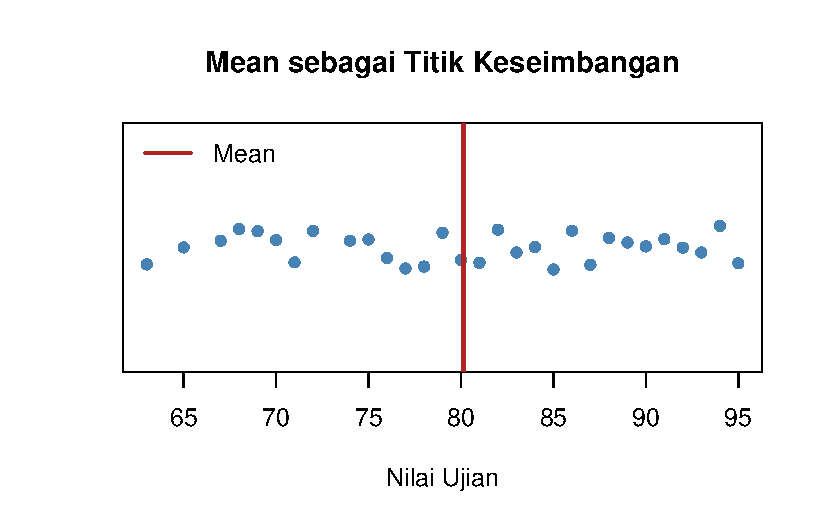
\includegraphics[keepaspectratio]{chapters/P05_files/figure-pdf/unnamed-chunk-6-1.pdf}}

\subsubsection{Rata-rata Tertimbang (Weighted
Mean)}\label{rata-rata-tertimbang-weighted-mean}

Jika setiap nilai memiliki bobot yang berbeda, gunakan rata-rata
tertimbang:

\[\bar{x}_w = \frac{\sum_{i=1}^{n} w_i x_i}{\sum_{i=1}^{n} w_i}\]

Contoh: IPK semester dihitung dari nilai mutu yang dibobot dengan jumlah
SKS.

\begin{Shaded}
\begin{Highlighting}[]
\NormalTok{mata\_kuliah }\OtherTok{\textless{}{-}} \FunctionTok{c}\NormalTok{(}\StringTok{"Statistika"}\NormalTok{, }\StringTok{"Kalkulus"}\NormalTok{, }\StringTok{"Basis Data"}\NormalTok{, }\StringTok{"Algoritma"}\NormalTok{)}
\NormalTok{nilai\_mutu }\OtherTok{\textless{}{-}} \FunctionTok{c}\NormalTok{(}\FloatTok{4.0}\NormalTok{, }\FloatTok{3.0}\NormalTok{, }\FloatTok{3.5}\NormalTok{, }\FloatTok{2.0}\NormalTok{)}
\NormalTok{sks }\OtherTok{\textless{}{-}} \FunctionTok{c}\NormalTok{(}\DecValTok{3}\NormalTok{, }\DecValTok{4}\NormalTok{, }\DecValTok{3}\NormalTok{, }\DecValTok{2}\NormalTok{)}
\NormalTok{knitr}\SpecialCharTok{::}\FunctionTok{kable}\NormalTok{(}\FunctionTok{data.frame}\NormalTok{(}\AttributeTok{Mata\_Kuliah =}\NormalTok{ mata\_kuliah, }\AttributeTok{Nilai\_Mutu =}\NormalTok{ nilai\_mutu, }\AttributeTok{SKS =}\NormalTok{ sks),}
\AttributeTok{caption =} \StringTok{"Data IPK Semester"}\NormalTok{)}
\end{Highlighting}
\end{Shaded}

\begin{longtable}[]{@{}lrr@{}}
\caption{Data IPK Semester}\tabularnewline
\toprule\noalign{}
Mata\_Kuliah & Nilai\_Mutu & SKS \\
\midrule\noalign{}
\endfirsthead
\toprule\noalign{}
Mata\_Kuliah & Nilai\_Mutu & SKS \\
\midrule\noalign{}
\endhead
\bottomrule\noalign{}
\endlastfoot
Statistika & 4.0 & 3 \\
Kalkulus & 3.0 & 4 \\
Basis Data & 3.5 & 3 \\
Algoritma & 2.0 & 2 \\
\end{longtable}

\begin{Shaded}
\begin{Highlighting}[]
\FunctionTok{mean}\NormalTok{(nilai\_mutu)                    }\CommentTok{\# rata{-}rata biasa (mengabaikan bobot SKS)}
\end{Highlighting}
\end{Shaded}

\begin{verbatim}
[1] 3.125
\end{verbatim}

\begin{Shaded}
\begin{Highlighting}[]
\FunctionTok{weighted.mean}\NormalTok{(nilai\_mutu, }\AttributeTok{w =}\NormalTok{ sks)  }\CommentTok{\# IPK sebenarnya}
\end{Highlighting}
\end{Shaded}

\begin{verbatim}
[1] 3.208333
\end{verbatim}

Rata-rata biasa (3,125) mengabaikan fakta bahwa Kalkulus (4 SKS) lebih
``berat'' daripada Algoritma (2 SKS). IPK yang benar adalah rata-rata
tertimbang, yaitu \textbf{3.208}.

\subsection{Median}\label{median}

Median adalah nilai tengah setelah data diurutkan. Median membagi data
menjadi dua bagian sama banyak: 50\% data berada di bawahnya dan 50\% di
atasnya.

\begin{itemize}
\tightlist
\item
  Jika \(n\) \textbf{ganjil}: median = data ke-\(\frac{n+1}{2}\).
\item
  Jika \(n\) \textbf{genap}: median = rata-rata data ke-\(\frac{n}{2}\)
  dan ke-\((\frac{n}{2}+1)\).
\end{itemize}

\begin{Shaded}
\begin{Highlighting}[]
\CommentTok{\# n = 30 (genap): rata{-}rata data ke{-}15 dan ke{-}16}
\NormalTok{urut }\OtherTok{\textless{}{-}} \FunctionTok{sort}\NormalTok{(nilai\_ujian)}
\NormalTok{urut[}\FunctionTok{c}\NormalTok{(}\DecValTok{15}\NormalTok{, }\DecValTok{16}\NormalTok{)]}
\end{Highlighting}
\end{Shaded}

\begin{verbatim}
[1] 80 81
\end{verbatim}

\begin{Shaded}
\begin{Highlighting}[]
\FunctionTok{mean}\NormalTok{(urut[}\FunctionTok{c}\NormalTok{(}\DecValTok{15}\NormalTok{, }\DecValTok{16}\NormalTok{)])}
\end{Highlighting}
\end{Shaded}

\begin{verbatim}
[1] 80.5
\end{verbatim}

\begin{Shaded}
\begin{Highlighting}[]
\FunctionTok{median}\NormalTok{(nilai\_ujian)}
\end{Highlighting}
\end{Shaded}

\begin{verbatim}
[1] 80.5
\end{verbatim}

Sekarang perhatikan data yang berbeda: gaji bulanan 7 karyawan sebuah
perusahaan rintisan (juta rupiah), di mana salah satunya adalah pendiri
perusahaan.

\begin{Shaded}
\begin{Highlighting}[]
\NormalTok{gaji }\OtherTok{\textless{}{-}} \FunctionTok{c}\NormalTok{(}\FloatTok{4.5}\NormalTok{, }\FloatTok{4.8}\NormalTok{, }\FloatTok{5.0}\NormalTok{, }\FloatTok{5.2}\NormalTok{, }\FloatTok{5.5}\NormalTok{, }\FloatTok{5.8}\NormalTok{, }\DecValTok{45}\NormalTok{)}
\CommentTok{\# n = 7 (ganjil): median = data ke{-}4}
\FunctionTok{sort}\NormalTok{(gaji)[}\DecValTok{4}\NormalTok{]}
\end{Highlighting}
\end{Shaded}

\begin{verbatim}
[1] 5.2
\end{verbatim}

\begin{Shaded}
\begin{Highlighting}[]
\FunctionTok{median}\NormalTok{(gaji)}
\end{Highlighting}
\end{Shaded}

\begin{verbatim}
[1] 5.2
\end{verbatim}

\begin{Shaded}
\begin{Highlighting}[]
\FunctionTok{mean}\NormalTok{(gaji)}
\end{Highlighting}
\end{Shaded}

\begin{verbatim}
[1] 10.82857
\end{verbatim}

Mean (10,83 juta) jauh lebih besar dari gaji enam dari tujuh karyawan,
karena tertarik oleh satu nilai ekstrem (45 juta). Median (5,2 juta)
\textbf{tidak terpengaruh besarnya} nilai ekstrem tersebut -- median
hanya peduli pada urutan, bukan besar nilainya. Inilah sebabnya median
disebut ukuran yang \textbf{tahan (robust)} terhadap outlier.

\subsubsection{Trimmed Mean: Jalan
Tengah}\label{trimmed-mean-jalan-tengah}

Trimmed mean membuang sebagian persentase data terkecil dan terbesar
sebelum menghitung rata-rata, sehingga tetap memakai banyak data tetapi
lebih tahan terhadap outlier.

\begin{Shaded}
\begin{Highlighting}[]
\FunctionTok{mean}\NormalTok{(gaji)                }\CommentTok{\# mean biasa}
\end{Highlighting}
\end{Shaded}

\begin{verbatim}
[1] 10.82857
\end{verbatim}

\begin{Shaded}
\begin{Highlighting}[]
\FunctionTok{mean}\NormalTok{(gaji, }\AttributeTok{trim =} \FloatTok{0.2}\NormalTok{)    }\CommentTok{\# buang 20\% terkecil \& 20\% terbesar (1 data tiap ujung)}
\end{Highlighting}
\end{Shaded}

\begin{verbatim}
[1] 5.26
\end{verbatim}

\begin{Shaded}
\begin{Highlighting}[]
\FunctionTok{median}\NormalTok{(gaji)              }\CommentTok{\# trimmed mean ekstrem (trim = 0.5)}
\end{Highlighting}
\end{Shaded}

\begin{verbatim}
[1] 5.2
\end{verbatim}

\subsection{Modus}\label{modus}

Modus adalah nilai yang \textbf{paling sering muncul}. Berbeda dengan
mean dan median, modus juga valid untuk data \textbf{nominal}. R tidak
menyediakan fungsi bawaan untuk modus statistik (fungsi \texttt{mode()}
di R menunjukkan tipe data, bukan modus), sehingga kita membuatnya
sendiri:

\begin{Shaded}
\begin{Highlighting}[]
\NormalTok{hitung\_modus }\OtherTok{\textless{}{-}} \ControlFlowTok{function}\NormalTok{(x) \{}
\NormalTok{tabel }\OtherTok{\textless{}{-}} \FunctionTok{table}\NormalTok{(x)}
\NormalTok{maks }\OtherTok{\textless{}{-}} \FunctionTok{max}\NormalTok{(tabel)}
\ControlFlowTok{if}\NormalTok{ (maks }\SpecialCharTok{==} \DecValTok{1}\NormalTok{) }\FunctionTok{return}\NormalTok{(}\ConstantTok{NA}\NormalTok{)                     }\CommentTok{\# semua nilai unik {-}\textgreater{} tidak ada modus}
\NormalTok{hasil }\OtherTok{\textless{}{-}} \FunctionTok{names}\NormalTok{(tabel)[tabel }\SpecialCharTok{==}\NormalTok{ maks]          }\CommentTok{\# bisa lebih dari satu modus}
\ControlFlowTok{if}\NormalTok{ (}\FunctionTok{is.numeric}\NormalTok{(x)) }\FunctionTok{as.numeric}\NormalTok{(hasil) }\ControlFlowTok{else}\NormalTok{ hasil}
\NormalTok{\}}

\FunctionTok{hitung\_modus}\NormalTok{(}\FunctionTok{c}\NormalTok{(}\DecValTok{2}\NormalTok{, }\DecValTok{3}\NormalTok{, }\DecValTok{3}\NormalTok{, }\DecValTok{4}\NormalTok{, }\DecValTok{4}\NormalTok{, }\DecValTok{4}\NormalTok{, }\DecValTok{5}\NormalTok{))   }\CommentTok{\# satu modus (unimodal)}
\end{Highlighting}
\end{Shaded}

\begin{verbatim}
[1] 4
\end{verbatim}

\begin{Shaded}
\begin{Highlighting}[]
\FunctionTok{hitung\_modus}\NormalTok{(}\FunctionTok{c}\NormalTok{(}\DecValTok{1}\NormalTok{, }\DecValTok{2}\NormalTok{, }\DecValTok{2}\NormalTok{, }\DecValTok{3}\NormalTok{, }\DecValTok{3}\NormalTok{, }\DecValTok{4}\NormalTok{))      }\CommentTok{\# dua modus (bimodal)}
\end{Highlighting}
\end{Shaded}

\begin{verbatim}
[1] 2 3
\end{verbatim}

\begin{Shaded}
\begin{Highlighting}[]
\FunctionTok{hitung\_modus}\NormalTok{(nilai\_ujian)              }\CommentTok{\# tidak ada modus (semua nilai unik)}
\end{Highlighting}
\end{Shaded}

\begin{verbatim}
[1] NA
\end{verbatim}

\begin{Shaded}
\begin{Highlighting}[]
\CommentTok{\# Modus pada data nominal}
\NormalTok{metode\_bayar }\OtherTok{\textless{}{-}} \FunctionTok{c}\NormalTok{(}\StringTok{"Tunai"}\NormalTok{, }\StringTok{"Debit"}\NormalTok{, }\StringTok{"Debit"}\NormalTok{, }\StringTok{"E{-}Wallet"}\NormalTok{, }\StringTok{"Debit"}\NormalTok{, }\StringTok{"Kredit"}\NormalTok{, }\StringTok{"Tunai"}\NormalTok{)}
\FunctionTok{hitung\_modus}\NormalTok{(metode\_bayar)}
\end{Highlighting}
\end{Shaded}

\begin{verbatim}
[1] "Debit"
\end{verbatim}

\textbf{Catatan:} untuk data kontinu (seperti nilai ujian di atas) yang
hampir tidak pernah berulang persis, modus dari data mentah tidak
informatif. Solusinya adalah mencari \textbf{kelas modus} dari data yang
sudah dikelompokkan (dibahas pada bagian Data Terkelompok).

\subsection{Membandingkan dan Memilih Ukuran
Pemusatan}\label{membandingkan-dan-memilih-ukuran-pemusatan}

{\def\LTcaptype{none} % do not increment counter
\begin{longtable}[]{@{}
  >{\raggedright\arraybackslash}p{(\linewidth - 6\tabcolsep) * \real{0.2500}}
  >{\raggedright\arraybackslash}p{(\linewidth - 6\tabcolsep) * \real{0.2500}}
  >{\raggedright\arraybackslash}p{(\linewidth - 6\tabcolsep) * \real{0.2500}}
  >{\raggedright\arraybackslash}p{(\linewidth - 6\tabcolsep) * \real{0.2500}}@{}}
\toprule\noalign{}
\begin{minipage}[b]{\linewidth}\raggedright
Ukuran
\end{minipage} & \begin{minipage}[b]{\linewidth}\raggedright
Kelebihan
\end{minipage} & \begin{minipage}[b]{\linewidth}\raggedright
Kelemahan
\end{minipage} & \begin{minipage}[b]{\linewidth}\raggedright
Paling cocok untuk
\end{minipage} \\
\midrule\noalign{}
\endhead
\bottomrule\noalign{}
\endlastfoot
\textbf{Mean} & Memakai semua data; dasar bagi banyak metode statistik
lanjutan & Sensitif terhadap outlier dan data menceng & Data numerik
simetris tanpa outlier \\
\textbf{Median} & Tahan terhadap outlier; selalu ada & Tidak memakai
besar nilai semua data & Data numerik menceng (misalnya pendapatan,
harga rumah), atau data ordinal \\
\textbf{Modus} & Bisa untuk data nominal; mudah dipahami & Bisa tidak
ada atau lebih dari satu & Data nominal/kategorik; mencari nilai
terpopuler \\
\end{longtable}
}

\begin{Shaded}
\begin{Highlighting}[]
\FunctionTok{stripchart}\NormalTok{(gaji, }\AttributeTok{method =} \StringTok{"stack"}\NormalTok{, }\AttributeTok{pch =} \DecValTok{16}\NormalTok{, }\AttributeTok{cex =} \FloatTok{1.6}\NormalTok{, }\AttributeTok{col =} \StringTok{"steelblue"}\NormalTok{,}
\AttributeTok{xlim =} \FunctionTok{c}\NormalTok{(}\DecValTok{0}\NormalTok{, }\DecValTok{50}\NormalTok{), }\AttributeTok{xlab =} \StringTok{"Gaji Bulanan (Juta Rupiah)"}\NormalTok{,}
\AttributeTok{main =} \StringTok{"Mean Tertarik ke Arah Outlier, Median Tidak"}\NormalTok{)}
\FunctionTok{abline}\NormalTok{(}\AttributeTok{v =} \FunctionTok{mean}\NormalTok{(gaji),              }\AttributeTok{col =} \StringTok{"firebrick"}\NormalTok{,  }\AttributeTok{lwd =} \DecValTok{2}\NormalTok{)}
\FunctionTok{abline}\NormalTok{(}\AttributeTok{v =} \FunctionTok{median}\NormalTok{(gaji),            }\AttributeTok{col =} \StringTok{"darkgreen"}\NormalTok{,  }\AttributeTok{lwd =} \DecValTok{2}\NormalTok{, }\AttributeTok{lty =} \DecValTok{2}\NormalTok{)}
\FunctionTok{abline}\NormalTok{(}\AttributeTok{v =} \FunctionTok{mean}\NormalTok{(gaji, }\AttributeTok{trim =} \FloatTok{0.2}\NormalTok{),  }\AttributeTok{col =} \StringTok{"darkorange"}\NormalTok{, }\AttributeTok{lwd =} \DecValTok{2}\NormalTok{, }\AttributeTok{lty =} \DecValTok{3}\NormalTok{)}
\FunctionTok{legend}\NormalTok{(}\StringTok{"topright"}\NormalTok{, }\AttributeTok{bty =} \StringTok{"n"}\NormalTok{, }\AttributeTok{lwd =} \DecValTok{2}\NormalTok{, }\AttributeTok{lty =} \FunctionTok{c}\NormalTok{(}\DecValTok{1}\NormalTok{, }\DecValTok{2}\NormalTok{, }\DecValTok{3}\NormalTok{),}
\AttributeTok{col =} \FunctionTok{c}\NormalTok{(}\StringTok{"firebrick"}\NormalTok{, }\StringTok{"darkgreen"}\NormalTok{, }\StringTok{"darkorange"}\NormalTok{),}
\AttributeTok{legend =} \FunctionTok{c}\NormalTok{(}\StringTok{"Mean"}\NormalTok{, }\StringTok{"Median"}\NormalTok{, }\StringTok{"Trimmed mean (20\%)"}\NormalTok{))}
\end{Highlighting}
\end{Shaded}

\pandocbounded{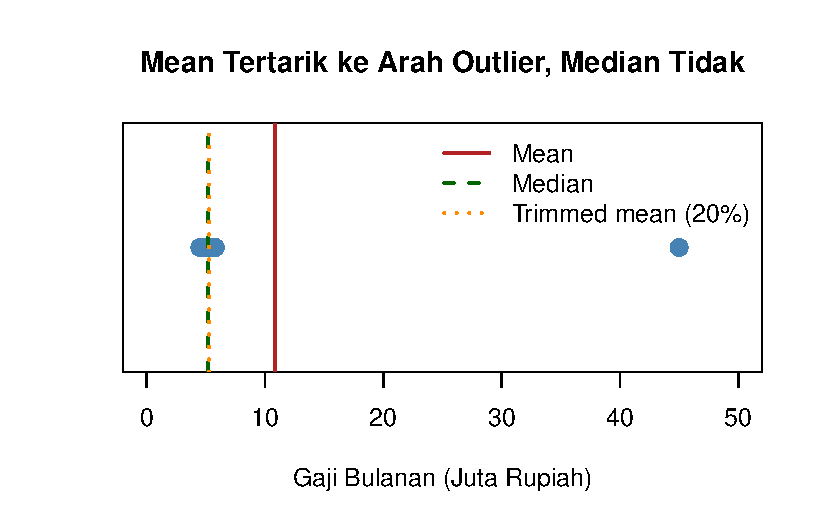
\includegraphics[keepaspectratio]{chapters/P05_files/figure-pdf/unnamed-chunk-14-1.pdf}}

\textbf{Panduan memilih:}

\begin{itemize}
\tightlist
\item
  Data \textbf{nominal} → gunakan \textbf{modus}.
\item
  Data \textbf{ordinal} → gunakan \textbf{median} (dan modus).
\item
  Data numerik \textbf{simetris, tanpa outlier} → \textbf{mean}.
\item
  Data numerik \textbf{menceng atau mengandung outlier} →
  \textbf{median} (laporkan mean sebagai pelengkap jika perlu).
\end{itemize}

\section{Catatan: Median sebagai Ukuran
Letak}\label{catatan-median-sebagai-ukuran-letak}

Median membagi data terurut menjadi dua bagian sama banyak. Gagasan yang
sama dapat diperluas menjadi \textbf{kuartil} (empat bagian),
\textbf{desil} (sepuluh bagian), dan \textbf{persentil} (seratus
bagian), beserta \textbf{rentang antarkuartil (IQR)} sebagai ukuran
sebaran yang tahan nilai ekstrem. Semua ukuran letak tersebut dibahas
lengkap pada \textbf{Pertemuan 6}. Untuk saat ini, cukup diingat bahwa
median adalah \textbf{persentil ke-50}.

\section{Ukuran Penyebaran Data}\label{ukuran-penyebaran-data}

\subsection{Mengapa Ukuran Pusat Saja Tidak
Cukup?}\label{mengapa-ukuran-pusat-saja-tidak-cukup}

Dua loket pelayanan mencatat waktu tunggu (menit) enam pelanggan.
Keduanya memiliki mean dan median yang persis sama:

\begin{Shaded}
\begin{Highlighting}[]
\NormalTok{loket\_1 }\OtherTok{\textless{}{-}} \FunctionTok{c}\NormalTok{(}\DecValTok{9}\NormalTok{, }\DecValTok{10}\NormalTok{, }\DecValTok{10}\NormalTok{, }\DecValTok{10}\NormalTok{, }\DecValTok{10}\NormalTok{, }\DecValTok{11}\NormalTok{)}
\NormalTok{loket\_2 }\OtherTok{\textless{}{-}} \FunctionTok{c}\NormalTok{(}\DecValTok{1}\NormalTok{, }\DecValTok{4}\NormalTok{, }\DecValTok{10}\NormalTok{, }\DecValTok{10}\NormalTok{, }\DecValTok{16}\NormalTok{, }\DecValTok{19}\NormalTok{)}

\FunctionTok{rbind}\NormalTok{(}\AttributeTok{Loket\_1 =} \FunctionTok{c}\NormalTok{(}\AttributeTok{Mean =} \FunctionTok{mean}\NormalTok{(loket\_1), }\AttributeTok{Median =} \FunctionTok{median}\NormalTok{(loket\_1)),}
\AttributeTok{Loket\_2 =} \FunctionTok{c}\NormalTok{(}\AttributeTok{Mean =} \FunctionTok{mean}\NormalTok{(loket\_2), }\AttributeTok{Median =} \FunctionTok{median}\NormalTok{(loket\_2)))}
\end{Highlighting}
\end{Shaded}

\begin{verbatim}
        Mean Median
Loket_1   10     10
Loket_2   10     10
\end{verbatim}

\begin{Shaded}
\begin{Highlighting}[]
\FunctionTok{par}\NormalTok{(}\AttributeTok{mfrow =} \FunctionTok{c}\NormalTok{(}\DecValTok{1}\NormalTok{, }\DecValTok{2}\NormalTok{))}
\FunctionTok{stripchart}\NormalTok{(loket\_1, }\AttributeTok{method =} \StringTok{"stack"}\NormalTok{, }\AttributeTok{pch =} \DecValTok{16}\NormalTok{, }\AttributeTok{cex =} \FloatTok{1.6}\NormalTok{, }\AttributeTok{col =} \StringTok{"steelblue"}\NormalTok{,}
\AttributeTok{xlim =} \FunctionTok{c}\NormalTok{(}\DecValTok{0}\NormalTok{, }\DecValTok{20}\NormalTok{), }\AttributeTok{xlab =} \StringTok{"Waktu Tunggu (menit)"}\NormalTok{, }\AttributeTok{main =} \StringTok{"Loket 1"}\NormalTok{)}
\FunctionTok{abline}\NormalTok{(}\AttributeTok{v =} \DecValTok{10}\NormalTok{, }\AttributeTok{col =} \StringTok{"firebrick"}\NormalTok{, }\AttributeTok{lwd =} \DecValTok{2}\NormalTok{)}
\FunctionTok{stripchart}\NormalTok{(loket\_2, }\AttributeTok{method =} \StringTok{"stack"}\NormalTok{, }\AttributeTok{pch =} \DecValTok{16}\NormalTok{, }\AttributeTok{cex =} \FloatTok{1.6}\NormalTok{, }\AttributeTok{col =} \StringTok{"darkorange"}\NormalTok{,}
\AttributeTok{xlim =} \FunctionTok{c}\NormalTok{(}\DecValTok{0}\NormalTok{, }\DecValTok{20}\NormalTok{), }\AttributeTok{xlab =} \StringTok{"Waktu Tunggu (menit)"}\NormalTok{, }\AttributeTok{main =} \StringTok{"Loket 2"}\NormalTok{)}
\FunctionTok{abline}\NormalTok{(}\AttributeTok{v =} \DecValTok{10}\NormalTok{, }\AttributeTok{col =} \StringTok{"firebrick"}\NormalTok{, }\AttributeTok{lwd =} \DecValTok{2}\NormalTok{)}
\end{Highlighting}
\end{Shaded}

\pandocbounded{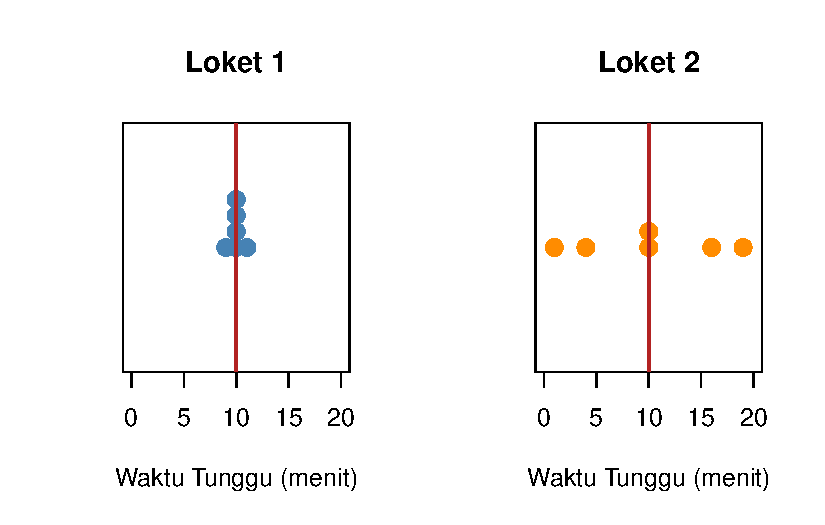
\includegraphics[keepaspectratio]{chapters/P05_files/figure-pdf/unnamed-chunk-16-1.pdf}}

\begin{Shaded}
\begin{Highlighting}[]
\FunctionTok{par}\NormalTok{(}\AttributeTok{mfrow =} \FunctionTok{c}\NormalTok{(}\DecValTok{1}\NormalTok{, }\DecValTok{1}\NormalTok{))}
\end{Highlighting}
\end{Shaded}

Kedua loket ``rata-rata 10 menit'', tetapi pengalaman pelanggannya
sangat berbeda: Loket 1 \textbf{konsisten}, Loket 2 \textbf{tidak dapat
diprediksi} (ada yang hanya menunggu 1 menit, ada yang 19 menit).
Perbedaan inilah yang ditangkap oleh ukuran penyebaran.

\subsection{Rentang (Range)}\label{rentang-range}

\[\text{Rentang} = x_{\text{max}} - x_{\text{min}}\]

\begin{Shaded}
\begin{Highlighting}[]
\FunctionTok{range}\NormalTok{(nilai\_ujian)              }\CommentTok{\# R mengembalikan nilai min dan max, BUKAN selisihnya}
\end{Highlighting}
\end{Shaded}

\begin{verbatim}
[1] 63 95
\end{verbatim}

\begin{Shaded}
\begin{Highlighting}[]
\FunctionTok{diff}\NormalTok{(}\FunctionTok{range}\NormalTok{(nilai\_ujian))        }\CommentTok{\# rentang sebenarnya}
\end{Highlighting}
\end{Shaded}

\begin{verbatim}
[1] 32
\end{verbatim}

\begin{Shaded}
\begin{Highlighting}[]
\FunctionTok{diff}\NormalTok{(}\FunctionTok{range}\NormalTok{(loket\_1))}
\end{Highlighting}
\end{Shaded}

\begin{verbatim}
[1] 2
\end{verbatim}

\begin{Shaded}
\begin{Highlighting}[]
\FunctionTok{diff}\NormalTok{(}\FunctionTok{range}\NormalTok{(loket\_2))}
\end{Highlighting}
\end{Shaded}

\begin{verbatim}
[1] 18
\end{verbatim}

Rentang mudah dihitung, tetapi hanya memakai \textbf{dua nilai}
(terkecil dan terbesar) sehingga sangat dipengaruhi nilai ekstrem dan
mengabaikan sebaran data di antaranya. Ukuran sebaran yang memakai
\textbf{seluruh} data adalah varians dan simpangan baku.

\subsection{Deviasi, Varians, dan Simpangan
Baku}\label{deviasi-varians-dan-simpangan-baku}

Untuk mengukur ``rata-rata jarak data dari meannya'', langkah pertama
yang terpikir adalah merata-ratakan deviasi \((x_i - \bar{x})\). Namun
sudah kita lihat bahwa jumlah deviasi selalu nol (yang positif dan
negatif saling meniadakan), sehingga tidak informatif. Ada dua jalan
keluar: memakai nilai mutlak (menghasilkan \emph{mean absolute
deviation}) atau \textbf{mengkuadratkan} deviasi (menghasilkan
\textbf{varians}). Cara kedua lebih umum karena sifat matematisnya yang
baik.

\textbf{Rumus varians:}

\[\sigma^2 = \frac{\sum_{i=1}^{N}(x_i - \mu)^2}{N} \qquad\qquad s^2 = \frac{\sum_{i=1}^{n}(x_i - \bar{x})^2}{n-1}\]

\textbf{Simpangan baku} (standar deviasi): akar dari varians, sehingga
satuannya kembali sama dengan data asli.

\[\sigma = \sqrt{\sigma^2} \qquad\qquad s = \sqrt{s^2}\]

\subsubsection{Langkah Perhitungan
Manual}\label{langkah-perhitungan-manual}

Contoh: skor kuis 8 mahasiswa (sampel).

\begin{Shaded}
\begin{Highlighting}[]
\NormalTok{kuis }\OtherTok{\textless{}{-}} \FunctionTok{c}\NormalTok{(}\DecValTok{6}\NormalTok{, }\DecValTok{8}\NormalTok{, }\DecValTok{7}\NormalTok{, }\DecValTok{9}\NormalTok{, }\DecValTok{5}\NormalTok{, }\DecValTok{10}\NormalTok{, }\DecValTok{7}\NormalTok{, }\DecValTok{8}\NormalTok{)}
\NormalTok{rata\_kuis }\OtherTok{\textless{}{-}} \FunctionTok{mean}\NormalTok{(kuis)}

\NormalTok{tabel\_deviasi }\OtherTok{\textless{}{-}} \FunctionTok{data.frame}\NormalTok{(}
\AttributeTok{x =}\NormalTok{ kuis,}
\AttributeTok{Deviasi =}\NormalTok{ kuis }\SpecialCharTok{{-}}\NormalTok{ rata\_kuis,}
\AttributeTok{Deviasi\_Kuadrat =}\NormalTok{ (kuis }\SpecialCharTok{{-}}\NormalTok{ rata\_kuis)}\SpecialCharTok{\^{}}\DecValTok{2}
\NormalTok{)}
\NormalTok{knitr}\SpecialCharTok{::}\FunctionTok{kable}\NormalTok{(tabel\_deviasi, }\AttributeTok{caption =} \FunctionTok{paste0}\NormalTok{(}\StringTok{"Tabel Deviasi (mean = "}\NormalTok{, rata\_kuis, }\StringTok{")"}\NormalTok{))}
\end{Highlighting}
\end{Shaded}

\begin{longtable}[]{@{}rrr@{}}
\caption{Tabel Deviasi (mean = 7.5)}\tabularnewline
\toprule\noalign{}
x & Deviasi & Deviasi\_Kuadrat \\
\midrule\noalign{}
\endfirsthead
\toprule\noalign{}
x & Deviasi & Deviasi\_Kuadrat \\
\midrule\noalign{}
\endhead
\bottomrule\noalign{}
\endlastfoot
6 & -1.5 & 2.25 \\
8 & 0.5 & 0.25 \\
7 & -0.5 & 0.25 \\
9 & 1.5 & 2.25 \\
5 & -2.5 & 6.25 \\
10 & 2.5 & 6.25 \\
7 & -0.5 & 0.25 \\
8 & 0.5 & 0.25 \\
\end{longtable}

\begin{Shaded}
\begin{Highlighting}[]
\FunctionTok{colSums}\NormalTok{(tabel\_deviasi)   }\CommentTok{\# jumlah deviasi = 0; jumlah kuadrat deviasi = 18}
\end{Highlighting}
\end{Shaded}

\begin{verbatim}
              x         Deviasi Deviasi_Kuadrat 
             60               0              18 
\end{verbatim}

\begin{Shaded}
\begin{Highlighting}[]
\NormalTok{n\_k }\OtherTok{\textless{}{-}} \FunctionTok{length}\NormalTok{(kuis)}
\NormalTok{JKD }\OtherTok{\textless{}{-}} \FunctionTok{sum}\NormalTok{((kuis }\SpecialCharTok{{-}} \FunctionTok{mean}\NormalTok{(kuis))}\SpecialCharTok{\^{}}\DecValTok{2}\NormalTok{)             }\CommentTok{\# jumlah kuadrat deviasi}
\FunctionTok{c}\NormalTok{(}\AttributeTok{Varians\_Sampel =}\NormalTok{ JKD }\SpecialCharTok{/}\NormalTok{ (n\_k }\SpecialCharTok{{-}} \DecValTok{1}\NormalTok{),           }\CommentTok{\# s\^{}2 (dibagi n {-} 1)}
\AttributeTok{Varians\_Populasi =}\NormalTok{ JKD }\SpecialCharTok{/}\NormalTok{ n\_k,               }\CommentTok{\# sigma\^{}2 (dibagi N)}
\AttributeTok{SD\_Sampel =} \FunctionTok{sqrt}\NormalTok{(JKD }\SpecialCharTok{/}\NormalTok{ (n\_k }\SpecialCharTok{{-}} \DecValTok{1}\NormalTok{)))}
\end{Highlighting}
\end{Shaded}

\begin{verbatim}
  Varians_Sampel Varians_Populasi        SD_Sampel 
        2.571429         2.250000         1.603567 
\end{verbatim}

\begin{Shaded}
\begin{Highlighting}[]
\FunctionTok{var}\NormalTok{(kuis)   }\CommentTok{\# fungsi bawaan R}
\end{Highlighting}
\end{Shaded}

\begin{verbatim}
[1] 2.571429
\end{verbatim}

\begin{Shaded}
\begin{Highlighting}[]
\FunctionTok{sd}\NormalTok{(kuis)    }\CommentTok{\# fungsi bawaan R}
\end{Highlighting}
\end{Shaded}

\begin{verbatim}
[1] 1.603567
\end{verbatim}

\begin{Shaded}
\begin{Highlighting}[]
\CommentTok{\# Rumus komputasi (setara): [sum(x\^{}2) {-} (sum(x))\^{}2 / n] / (n {-} 1)}
\NormalTok{(}\FunctionTok{sum}\NormalTok{(kuis}\SpecialCharTok{\^{}}\DecValTok{2}\NormalTok{) }\SpecialCharTok{{-}} \FunctionTok{sum}\NormalTok{(kuis)}\SpecialCharTok{\^{}}\DecValTok{2} \SpecialCharTok{/}\NormalTok{ n\_k) }\SpecialCharTok{/}\NormalTok{ (n\_k }\SpecialCharTok{{-}} \DecValTok{1}\NormalTok{)}
\end{Highlighting}
\end{Shaded}

\begin{verbatim}
[1] 2.571429
\end{verbatim}

Jadi \(s^2 = \frac{18}{7} \approx 2{,}571\) dan
\(s = \sqrt{2{,}571} \approx 1{,}604\). Secara sederhana, skor kuis
rata-rata menyimpang sekitar 1,6 poin dari meannya.

\begin{quote}
\textbf{Awas:} fungsi \texttt{var()} dan \texttt{sd()} di R
\textbf{selalu} membagi dengan \(n-1\) (versi sampel). Jika data Anda
adalah seluruh populasi, gunakan \texttt{mean((x\ -\ mean(x))\^{}2)}
untuk varians populasi.
\end{quote}

\subsubsection{\texorpdfstring{Mengapa Dibagi
\(n-1\)?}{Mengapa Dibagi n-1?}}\label{mengapa-dibagi-n-1}

Deviasi dihitung terhadap \(\bar{x}\) (bukan \(\mu\) yang sebenarnya),
dan \(\bar{x}\) selalu ``menyesuaikan diri'' dengan sampel sehingga
jumlah kuadrat deviasinya cenderung \textbf{terlalu kecil}. Pembagian
dengan \(n-1\) (disebut \textbf{koreksi Bessel}, terkait \emph{derajat
bebas}) mengoreksi bias tersebut. Simulasi berikut membuktikannya:

\begin{Shaded}
\begin{Highlighting}[]
\FunctionTok{set.seed}\NormalTok{(}\DecValTok{2026}\NormalTok{)}
\NormalTok{populasi }\OtherTok{\textless{}{-}} \FunctionTok{rnorm}\NormalTok{(}\DecValTok{10000}\NormalTok{, }\AttributeTok{mean =} \DecValTok{50}\NormalTok{, }\AttributeTok{sd =} \DecValTok{10}\NormalTok{)}
\NormalTok{sigma2 }\OtherTok{\textless{}{-}} \FunctionTok{mean}\NormalTok{((populasi }\SpecialCharTok{{-}} \FunctionTok{mean}\NormalTok{(populasi))}\SpecialCharTok{\^{}}\DecValTok{2}\NormalTok{)   }\CommentTok{\# varians populasi sebenarnya}

\CommentTok{\# Ambil 5000 sampel berukuran n = 5, hitung varians dengan dua cara}
\NormalTok{hasil }\OtherTok{\textless{}{-}} \FunctionTok{replicate}\NormalTok{(}\DecValTok{5000}\NormalTok{, \{}
\NormalTok{s }\OtherTok{\textless{}{-}} \FunctionTok{sample}\NormalTok{(populasi, }\DecValTok{5}\NormalTok{)}
\FunctionTok{c}\NormalTok{(}\AttributeTok{bagi\_n =} \FunctionTok{sum}\NormalTok{((s }\SpecialCharTok{{-}} \FunctionTok{mean}\NormalTok{(s))}\SpecialCharTok{\^{}}\DecValTok{2}\NormalTok{) }\SpecialCharTok{/} \DecValTok{5}\NormalTok{, }\AttributeTok{bagi\_n\_min\_1 =} \FunctionTok{var}\NormalTok{(s))}
\NormalTok{\})}

\NormalTok{knitr}\SpecialCharTok{::}\FunctionTok{kable}\NormalTok{(}\FunctionTok{data.frame}\NormalTok{(}
\AttributeTok{Metode =} \FunctionTok{c}\NormalTok{(}\StringTok{"Varians populasi sebenarnya"}\NormalTok{, }\StringTok{"Rata{-}rata s\^{}2 dibagi n"}\NormalTok{, }\StringTok{"Rata{-}rata s\^{}2 dibagi n {-} 1"}\NormalTok{),}
\AttributeTok{Nilai =} \FunctionTok{round}\NormalTok{(}\FunctionTok{unname}\NormalTok{(}\FunctionTok{c}\NormalTok{(sigma2, }\FunctionTok{rowMeans}\NormalTok{(hasil))), }\DecValTok{2}\NormalTok{)}
\NormalTok{), }\AttributeTok{caption =} \StringTok{"Rata{-}rata dari 5000 varians sampel (n = 5)"}\NormalTok{)}
\end{Highlighting}
\end{Shaded}

\begin{longtable}[]{@{}lr@{}}
\caption{Rata-rata dari 5000 varians sampel (n = 5)}\tabularnewline
\toprule\noalign{}
Metode & Nilai \\
\midrule\noalign{}
\endfirsthead
\toprule\noalign{}
Metode & Nilai \\
\midrule\noalign{}
\endhead
\bottomrule\noalign{}
\endlastfoot
Varians populasi sebenarnya & 100.28 \\
Rata-rata s\^{}2 dibagi n & 79.45 \\
Rata-rata s\^{}2 dibagi n - 1 & 99.31 \\
\end{longtable}

Pembagian dengan \(n\) rata-rata menduga \textbf{terlalu rendah}
(sekitar 80\% dari nilai sebenarnya untuk \(n = 5\)), sedangkan
pembagian dengan \(n-1\) rata-rata tepat mendekati varians populasi
sebenarnya. Inilah sebab \(n-1\) dipakai untuk sampel.

\subsubsection{Menerapkan pada Data Nilai
Ujian}\label{menerapkan-pada-data-nilai-ujian}

\begin{Shaded}
\begin{Highlighting}[]
\FunctionTok{c}\NormalTok{(}\AttributeTok{Varians =} \FunctionTok{var}\NormalTok{(nilai\_ujian), }\AttributeTok{SD =} \FunctionTok{sd}\NormalTok{(nilai\_ujian))}
\end{Highlighting}
\end{Shaded}

\begin{verbatim}
  Varians        SD 
87.016092  9.328242 
\end{verbatim}

Simpangan baku nilai ujian sekitar \textbf{9.33} poin: secara umum,
nilai seorang mahasiswa menyimpang sekitar 9.3 poin dari rata-rata kelas
(80.1).

\subsection{Koefisien Variasi (CV)}\label{koefisien-variasi-cv}

Simpangan baku bergantung pada satuan dan besar data, sehingga tidak
adil untuk membandingkan variabilitas dua variabel yang skalanya
berbeda. \textbf{Koefisien variasi} menyatakan simpangan baku
\emph{relatif} terhadap meannya:

\[CV = \frac{s}{\bar{x}} \times 100\%\]

Contoh: manakah yang lebih bervariasi, tinggi badan atau berat badan
mahasiswa?

\begin{Shaded}
\begin{Highlighting}[]
\NormalTok{tinggi }\OtherTok{\textless{}{-}} \FunctionTok{c}\NormalTok{(}\AttributeTok{mean =} \DecValTok{165}\NormalTok{, }\AttributeTok{sd =} \DecValTok{8}\NormalTok{)   }\CommentTok{\# cm}
\NormalTok{berat  }\OtherTok{\textless{}{-}} \FunctionTok{c}\NormalTok{(}\AttributeTok{mean =} \DecValTok{60}\NormalTok{,  }\AttributeTok{sd =} \DecValTok{9}\NormalTok{)   }\CommentTok{\# kg}

\NormalTok{cv }\OtherTok{\textless{}{-}} \ControlFlowTok{function}\NormalTok{(rata, simpangan) simpangan }\SpecialCharTok{/}\NormalTok{ rata }\SpecialCharTok{*} \DecValTok{100}
\FunctionTok{c}\NormalTok{(}\AttributeTok{CV\_Tinggi\_persen =} \FunctionTok{cv}\NormalTok{(tinggi[[}\StringTok{"mean"}\NormalTok{]], tinggi[[}\StringTok{"sd"}\NormalTok{]]),}
\AttributeTok{CV\_Berat\_persen  =} \FunctionTok{cv}\NormalTok{(berat[[}\StringTok{"mean"}\NormalTok{]],  berat[[}\StringTok{"sd"}\NormalTok{]]))}
\end{Highlighting}
\end{Shaded}

\begin{verbatim}
CV_Tinggi_persen  CV_Berat_persen 
        4.848485        15.000000 
\end{verbatim}

Simpangan baku berat badan (9 kg) memang hanya sedikit lebih besar
daripada tinggi badan (8 cm), tetapi dalam kaitannya dengan meannya,
berat badan jauh lebih bervariatif (CV sekitar 15\% vs 4,8\%).
Perbandingan SD langsung antara ``cm'' dan ``kg'' tidak bermakna; CV
tidak memiliki satuan sehingga dapat dibandingkan.

\begin{quote}
\textbf{Syarat CV:} hanya valid untuk data \textbf{skala rasio} (nol
mutlak) dengan mean positif dan tidak mendekati nol. Jangan gunakan CV
untuk suhu dalam °C (skala interval).
\end{quote}

\subsection{Ringkasan Ukuran
Penyebaran}\label{ringkasan-ukuran-penyebaran}

{\def\LTcaptype{none} % do not increment counter
\begin{longtable}[]{@{}
  >{\raggedright\arraybackslash}p{(\linewidth - 8\tabcolsep) * \real{0.2000}}
  >{\raggedright\arraybackslash}p{(\linewidth - 8\tabcolsep) * \real{0.2000}}
  >{\raggedright\arraybackslash}p{(\linewidth - 8\tabcolsep) * \real{0.2000}}
  >{\raggedright\arraybackslash}p{(\linewidth - 8\tabcolsep) * \real{0.2000}}
  >{\raggedright\arraybackslash}p{(\linewidth - 8\tabcolsep) * \real{0.2000}}@{}}
\toprule\noalign{}
\begin{minipage}[b]{\linewidth}\raggedright
Ukuran
\end{minipage} & \begin{minipage}[b]{\linewidth}\raggedright
Rumus
\end{minipage} & \begin{minipage}[b]{\linewidth}\raggedright
Satuan
\end{minipage} & \begin{minipage}[b]{\linewidth}\raggedright
Tahan Outlier?
\end{minipage} & \begin{minipage}[b]{\linewidth}\raggedright
Berpasangan dengan
\end{minipage} \\
\midrule\noalign{}
\endhead
\bottomrule\noalign{}
\endlastfoot
Rentang & \(x_{\text{max}} - x_{\text{min}}\) & Sama dengan data & Tidak
& (Min, Maks) \\
Varians & \(\frac{\sum (x_i - \bar{x})^2}{n-1}\) & Kuadrat satuan data &
Tidak & Mean \\
Simpangan baku & \(\sqrt{s^2}\) & Sama dengan data & Tidak & Mean \\
Koefisien variasi & \(\frac{s}{\bar{x}} \times 100\%\) & Tanpa satuan
(\%) & Tidak & Membandingkan variabilitas relatif \\
\end{longtable}
}

\textbf{Kaidah pasangan:} mean dilaporkan bersama simpangan baku; median
dilaporkan bersama rentang atau -- setelah Pertemuan 6 -- bersama IQR
(kuartil).

\section{Interpretasi: Bentuk Distribusi dari Pusat dan
Sebaran}\label{interpretasi-bentuk-distribusi-dari-pusat-dan-sebaran}

Posisi relatif mean, median, dan modus mengungkap \textbf{bentuk
distribusi}:

{\def\LTcaptype{none} % do not increment counter
\begin{longtable}[]{@{}
  >{\raggedright\arraybackslash}p{(\linewidth - 4\tabcolsep) * \real{0.3333}}
  >{\raggedright\arraybackslash}p{(\linewidth - 4\tabcolsep) * \real{0.3333}}
  >{\raggedright\arraybackslash}p{(\linewidth - 4\tabcolsep) * \real{0.3333}}@{}}
\toprule\noalign{}
\begin{minipage}[b]{\linewidth}\raggedright
Bentuk
\end{minipage} & \begin{minipage}[b]{\linewidth}\raggedright
Ciri
\end{minipage} & \begin{minipage}[b]{\linewidth}\raggedright
Hubungan Mean--Median--Modus
\end{minipage} \\
\midrule\noalign{}
\endhead
\bottomrule\noalign{}
\endlastfoot
Simetris & Sisi kiri dan kanan saling mencerminkan & Mean ≈ Median ≈
Modus \\
Menjulur kanan (\emph{skewed right}) & Ekor panjang ke arah nilai besar
& Mean \textgreater{} Median \textgreater{} Modus \\
Menjulur kiri (\emph{skewed left}) & Ekor panjang ke arah nilai kecil &
Mean \textless{} Median \textless{} Modus \\
Bimodal & Dua puncak berbeda (kemungkinan dua sub-populasi) & Satu
ukuran pusat tidak cukup mewakili data \\
\end{longtable}
}

Mean paling ``tertarik'' ke arah ekor, sedangkan median lebih bertahan.
Karena itu selisih mean dan median dapat dijadikan petunjuk kemencengan.
Salah satu ukuran yang membakukannya adalah \textbf{koefisien
kemencengan Pearson}:

\[Sk = \frac{3(\bar{x} - \text{Median})}{s}\]

Aturan praktis: \(Sk > 0\) menjulur kanan, \(Sk < 0\) menjulur kiri, dan
\(|Sk|\) yang kecil (kurang dari sekitar 0,5) dianggap hampir simetris.

\begin{Shaded}
\begin{Highlighting}[]
\FunctionTok{set.seed}\NormalTok{(}\DecValTok{123}\NormalTok{)}
\NormalTok{data\_simetris     }\OtherTok{\textless{}{-}} \FunctionTok{rnorm}\NormalTok{(}\DecValTok{1000}\NormalTok{, }\AttributeTok{mean =} \DecValTok{50}\NormalTok{, }\AttributeTok{sd =} \DecValTok{10}\NormalTok{)}
\NormalTok{data\_skewed\_kanan }\OtherTok{\textless{}{-}} \FunctionTok{rbeta}\NormalTok{(}\DecValTok{1000}\NormalTok{, }\DecValTok{2}\NormalTok{, }\DecValTok{8}\NormalTok{) }\SpecialCharTok{*} \DecValTok{100}
\NormalTok{data\_bimodal      }\OtherTok{\textless{}{-}} \FunctionTok{c}\NormalTok{(}\FunctionTok{rnorm}\NormalTok{(}\DecValTok{500}\NormalTok{, }\AttributeTok{mean =} \DecValTok{30}\NormalTok{, }\AttributeTok{sd =} \DecValTok{5}\NormalTok{), }\FunctionTok{rnorm}\NormalTok{(}\DecValTok{500}\NormalTok{, }\AttributeTok{mean =} \DecValTok{70}\NormalTok{, }\AttributeTok{sd =} \DecValTok{5}\NormalTok{))}
\NormalTok{data\_skewed\_kiri  }\OtherTok{\textless{}{-}} \DecValTok{100} \SpecialCharTok{{-}} \FunctionTok{rbeta}\NormalTok{(}\DecValTok{1000}\NormalTok{, }\DecValTok{2}\NormalTok{, }\DecValTok{8}\NormalTok{) }\SpecialCharTok{*} \DecValTok{100}

\NormalTok{tampil\_hist }\OtherTok{\textless{}{-}} \ControlFlowTok{function}\NormalTok{(x, judul, warna, }\AttributeTok{dengan\_legenda =} \ConstantTok{FALSE}\NormalTok{) \{}
\FunctionTok{hist}\NormalTok{(x, }\AttributeTok{breaks =} \DecValTok{20}\NormalTok{, }\AttributeTok{col =}\NormalTok{ warna, }\AttributeTok{border =} \StringTok{"white"}\NormalTok{, }\AttributeTok{main =}\NormalTok{ judul,}
\AttributeTok{xlab =} \StringTok{"Nilai"}\NormalTok{, }\AttributeTok{ylab =} \StringTok{"Frekuensi"}\NormalTok{)}
\FunctionTok{abline}\NormalTok{(}\AttributeTok{v =} \FunctionTok{mean}\NormalTok{(x),   }\AttributeTok{col =} \StringTok{"red"}\NormalTok{,  }\AttributeTok{lwd =} \DecValTok{2}\NormalTok{)}
\FunctionTok{abline}\NormalTok{(}\AttributeTok{v =} \FunctionTok{median}\NormalTok{(x), }\AttributeTok{col =} \StringTok{"blue"}\NormalTok{, }\AttributeTok{lwd =} \DecValTok{2}\NormalTok{, }\AttributeTok{lty =} \DecValTok{2}\NormalTok{)}
\ControlFlowTok{if}\NormalTok{ (dengan\_legenda) \{}
\FunctionTok{legend}\NormalTok{(}\StringTok{"topright"}\NormalTok{, }\AttributeTok{legend =} \FunctionTok{c}\NormalTok{(}\StringTok{"Mean"}\NormalTok{, }\StringTok{"Median"}\NormalTok{), }\AttributeTok{col =} \FunctionTok{c}\NormalTok{(}\StringTok{"red"}\NormalTok{, }\StringTok{"blue"}\NormalTok{),}
\AttributeTok{lwd =} \DecValTok{2}\NormalTok{, }\AttributeTok{lty =} \FunctionTok{c}\NormalTok{(}\DecValTok{1}\NormalTok{, }\DecValTok{2}\NormalTok{), }\AttributeTok{bty =} \StringTok{"n"}\NormalTok{, }\AttributeTok{cex =} \FloatTok{0.8}\NormalTok{)}
\NormalTok{\}}
\NormalTok{\}}

\FunctionTok{par}\NormalTok{(}\AttributeTok{mfrow =} \FunctionTok{c}\NormalTok{(}\DecValTok{2}\NormalTok{, }\DecValTok{2}\NormalTok{))}
\FunctionTok{tampil\_hist}\NormalTok{(data\_simetris,     }\StringTok{"Simetris"}\NormalTok{,       }\StringTok{"steelblue"}\NormalTok{)}
\FunctionTok{tampil\_hist}\NormalTok{(data\_skewed\_kanan, }\StringTok{"Menjulur Kanan"}\NormalTok{, }\StringTok{"darkorange"}\NormalTok{, }\AttributeTok{dengan\_legenda =} \ConstantTok{TRUE}\NormalTok{)}
\FunctionTok{tampil\_hist}\NormalTok{(data\_skewed\_kiri,  }\StringTok{"Menjulur Kiri"}\NormalTok{,  }\StringTok{"purple3"}\NormalTok{)}
\FunctionTok{tampil\_hist}\NormalTok{(data\_bimodal,      }\StringTok{"Bimodal"}\NormalTok{,        }\StringTok{"seagreen"}\NormalTok{)}
\end{Highlighting}
\end{Shaded}

\pandocbounded{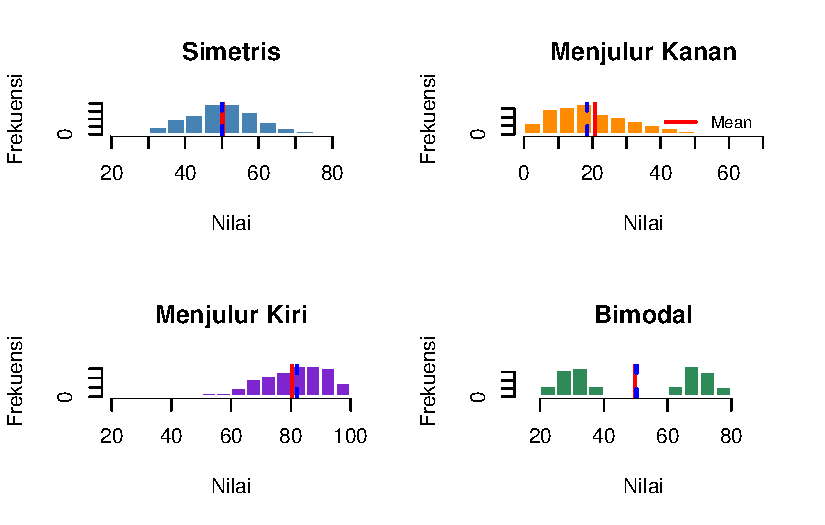
\includegraphics[keepaspectratio]{chapters/P05_files/figure-pdf/unnamed-chunk-24-1.pdf}}

\begin{Shaded}
\begin{Highlighting}[]
\FunctionTok{par}\NormalTok{(}\AttributeTok{mfrow =} \FunctionTok{c}\NormalTok{(}\DecValTok{1}\NormalTok{, }\DecValTok{1}\NormalTok{))}
\end{Highlighting}
\end{Shaded}

\begin{Shaded}
\begin{Highlighting}[]
\NormalTok{ringkas\_bentuk }\OtherTok{\textless{}{-}} \ControlFlowTok{function}\NormalTok{(x) \{}
\FunctionTok{c}\NormalTok{(}\AttributeTok{Mean =} \FunctionTok{mean}\NormalTok{(x), }\AttributeTok{Median =} \FunctionTok{median}\NormalTok{(x), }\AttributeTok{SD =} \FunctionTok{sd}\NormalTok{(x),}
\AttributeTok{Kemencengan\_Pearson =} \DecValTok{3} \SpecialCharTok{*}\NormalTok{ (}\FunctionTok{mean}\NormalTok{(x) }\SpecialCharTok{{-}} \FunctionTok{median}\NormalTok{(x)) }\SpecialCharTok{/} \FunctionTok{sd}\NormalTok{(x))}
\NormalTok{\}}

\NormalTok{knitr}\SpecialCharTok{::}\FunctionTok{kable}\NormalTok{(}\FunctionTok{round}\NormalTok{(}\FunctionTok{t}\NormalTok{(}\FunctionTok{sapply}\NormalTok{(}\FunctionTok{list}\NormalTok{(}\AttributeTok{Simetris =}\NormalTok{ data\_simetris, }\AttributeTok{Menjulur\_Kanan =}\NormalTok{ data\_skewed\_kanan,}
\AttributeTok{Menjulur\_Kiri =}\NormalTok{ data\_skewed\_kiri, }\AttributeTok{Bimodal =}\NormalTok{ data\_bimodal),}
\NormalTok{ringkas\_bentuk)), }\DecValTok{2}\NormalTok{),}
\AttributeTok{caption =} \StringTok{"Ukuran Pusat dan Kemencengan pada Empat Bentuk Distribusi"}\NormalTok{)}
\end{Highlighting}
\end{Shaded}

\begin{longtable}[]{@{}lrrrr@{}}
\caption{Ukuran Pusat dan Kemencengan pada Empat Bentuk
Distribusi}\tabularnewline
\toprule\noalign{}
& Mean & Median & SD & Kemencengan\_Pearson \\
\midrule\noalign{}
\endfirsthead
\toprule\noalign{}
& Mean & Median & SD & Kemencengan\_Pearson \\
\midrule\noalign{}
\endhead
\bottomrule\noalign{}
\endlastfoot
Simetris & 50.16 & 50.09 & 9.92 & 0.02 \\
Menjulur\_Kanan & 20.63 & 18.50 & 12.32 & 0.52 \\
Menjulur\_Kiri & 80.24 & 82.07 & 11.59 & -0.47 \\
Bimodal & 49.91 & 50.26 & 20.53 & -0.05 \\
\end{longtable}

\textbf{Interpretasi:}

\begin{itemize}
\tightlist
\item
  \textbf{Simetris:} mean dan median hampir sama; \(Sk \approx 0\).
\item
  \textbf{Menjulur kanan:} mean lebih besar dari median (ekor panjang di
  sisi nilai besar menarik mean); \(Sk > 0\).
\item
  \textbf{Menjulur kiri:} mean lebih kecil dari median; \(Sk < 0\).
\item
  \textbf{Bimodal:} mean dan median jatuh \textbf{di antara} dua puncak
  -- di wilayah yang hampir tidak ada datanya. Pada kasus ini,
  melaporkan ``rata-rata'' saja menyesatkan; sebaiknya pisahkan data
  menjadi dua kelompok atau laporkan kedua puncaknya.
\end{itemize}

\textbf{Latihan reflektif:} Bagaimana bentuk distribusi nilai ujian
Statistika (\texttt{nilai\_ujian})? Jawab dengan membandingkan mean dan
median-nya:

\begin{Shaded}
\begin{Highlighting}[]
\FunctionTok{c}\NormalTok{(}\AttributeTok{Mean =} \FunctionTok{mean}\NormalTok{(nilai\_ujian), }\AttributeTok{Median =} \FunctionTok{median}\NormalTok{(nilai\_ujian),}
\AttributeTok{Kemencengan\_Pearson =} \DecValTok{3} \SpecialCharTok{*}\NormalTok{ (}\FunctionTok{mean}\NormalTok{(nilai\_ujian) }\SpecialCharTok{{-}} \FunctionTok{median}\NormalTok{(nilai\_ujian)) }\SpecialCharTok{/} \FunctionTok{sd}\NormalTok{(nilai\_ujian))}
\end{Highlighting}
\end{Shaded}

\begin{verbatim}
               Mean              Median Kemencengan_Pearson 
         80.1333333          80.5000000          -0.1179215 
\end{verbatim}

\textbf{Jawaban:} mean (80.13) dan median (80.5) hampir sama dan \(Sk\)
mendekati nol, sehingga distribusinya \textbf{relatif simetris} --
konsisten dengan bentuk histogram pada awal praktikum.

\section{Interpretasi: Pengaruh Nilai
Ekstrem}\label{interpretasi-pengaruh-nilai-ekstrem}

Kita sudah melihat pada data gaji bahwa satu nilai ekstrem dapat menarik
mean jauh dari ``kebanyakan'' data. Bagaimana dengan ukuran penyebaran?

\subsection{Ukuran Mana yang Tahan Nilai
Ekstrem?}\label{ukuran-mana-yang-tahan-nilai-ekstrem}

Bandingkan seluruh ukuran pada data gaji \textbf{dengan} dan
\textbf{tanpa} outlier:

\begin{Shaded}
\begin{Highlighting}[]
\NormalTok{ukuran }\OtherTok{\textless{}{-}} \ControlFlowTok{function}\NormalTok{(x) \{}
\FunctionTok{c}\NormalTok{(}\AttributeTok{Mean =} \FunctionTok{mean}\NormalTok{(x), }\AttributeTok{Median =} \FunctionTok{median}\NormalTok{(x), }\AttributeTok{SD =} \FunctionTok{sd}\NormalTok{(x),}
\AttributeTok{Rentang =} \FunctionTok{diff}\NormalTok{(}\FunctionTok{range}\NormalTok{(x)), }\AttributeTok{CV\_persen =} \FunctionTok{sd}\NormalTok{(x) }\SpecialCharTok{/} \FunctionTok{mean}\NormalTok{(x) }\SpecialCharTok{*} \DecValTok{100}\NormalTok{)}
\NormalTok{\}}

\NormalTok{gaji\_tanpa\_outlier }\OtherTok{\textless{}{-}}\NormalTok{ gaji[gaji }\SpecialCharTok{!=} \FunctionTok{max}\NormalTok{(gaji)]}

\NormalTok{knitr}\SpecialCharTok{::}\FunctionTok{kable}\NormalTok{(}\FunctionTok{round}\NormalTok{(}\FunctionTok{rbind}\NormalTok{(}\StringTok{"Dengan outlier"} \OtherTok{=} \FunctionTok{ukuran}\NormalTok{(gaji),}
\StringTok{"Tanpa outlier"}  \OtherTok{=} \FunctionTok{ukuran}\NormalTok{(gaji\_tanpa\_outlier)), }\DecValTok{2}\NormalTok{),}
\AttributeTok{caption =} \StringTok{"Pengaruh Satu Nilai Ekstrem terhadap Ukuran Pusat dan Sebaran"}\NormalTok{)}
\end{Highlighting}
\end{Shaded}

\begin{longtable}[]{@{}lrrrrr@{}}
\caption{Pengaruh Satu Nilai Ekstrem terhadap Ukuran Pusat dan
Sebaran}\tabularnewline
\toprule\noalign{}
& Mean & Median & SD & Rentang & CV\_persen \\
\midrule\noalign{}
\endfirsthead
\toprule\noalign{}
& Mean & Median & SD & Rentang & CV\_persen \\
\midrule\noalign{}
\endhead
\bottomrule\noalign{}
\endlastfoot
Dengan outlier & 10.83 & 5.2 & 15.07 & 40.5 & 139.21 \\
Tanpa outlier & 5.13 & 5.1 & 0.47 & 1.3 & 9.19 \\
\end{longtable}

Satu data ekstrem mengubah \textbf{mean, SD, rentang, dan CV} secara
dramatis, sedangkan \textbf{median} hampir tidak berubah. Ringkasnya:

{\def\LTcaptype{none} % do not increment counter
\begin{longtable}[]{@{}
  >{\raggedright\arraybackslash}p{(\linewidth - 4\tabcolsep) * \real{0.3333}}
  >{\raggedright\arraybackslash}p{(\linewidth - 4\tabcolsep) * \real{0.3333}}
  >{\raggedright\arraybackslash}p{(\linewidth - 4\tabcolsep) * \real{0.3333}}@{}}
\toprule\noalign{}
\begin{minipage}[b]{\linewidth}\raggedright
\end{minipage} & \begin{minipage}[b]{\linewidth}\raggedright
Tidak tahan outlier
\end{minipage} & \begin{minipage}[b]{\linewidth}\raggedright
Tahan outlier (robust)
\end{minipage} \\
\midrule\noalign{}
\endhead
\bottomrule\noalign{}
\endlastfoot
Ukuran pusat & Mean & Median, trimmed mean \\
Ukuran sebaran & Rentang, varians, simpangan baku, CV & IQR (Pertemuan
6) \\
\end{longtable}
}

\begin{quote}
Cara mendeteksi outlier secara formal (pagar IQR, boxplot,
\emph{modified z-score}) dibahas pada Pertemuan 6. Satu prinsip yang
perlu dipegang sejak sekarang -- \textbf{jangan menghapus nilai ekstrem
secara otomatis}. Selidiki dahulu penyebabnya: (1) kesalahan
input/pengukuran → perbaiki atau hapus; (2) nilai ekstrem yang sah
(seperti gaji pendiri perusahaan) → pertahankan, dan gunakan ukuran yang
robust; (3) berasal dari populasi yang berbeda → analisis terpisah.
Selalu laporkan keputusan Anda.
\end{quote}

\section{Interpretasi: Menafsirkan Simpangan
Baku}\label{interpretasi-menafsirkan-simpangan-baku}

\subsection{Z-Score}\label{z-score}

Z-score menyatakan berapa simpangan baku sebuah nilai berada di atas (+)
atau di bawah (−) mean:

\[z = \frac{x - \bar{x}}{s}\]

Karena tanpa satuan, z-score memungkinkan membandingkan nilai dari skala
yang berbeda.

\begin{Shaded}
\begin{Highlighting}[]
\NormalTok{z\_ujian }\OtherTok{\textless{}{-}}\NormalTok{ (nilai\_ujian }\SpecialCharTok{{-}} \FunctionTok{mean}\NormalTok{(nilai\_ujian)) }\SpecialCharTok{/} \FunctionTok{sd}\NormalTok{(nilai\_ujian)   }\CommentTok{\# setara scale(nilai\_ujian)}

\FunctionTok{round}\NormalTok{(}\FunctionTok{c}\NormalTok{(}\AttributeTok{Nilai\_63 =}\NormalTok{ z\_ujian[nilai\_ujian }\SpecialCharTok{==} \DecValTok{63}\NormalTok{],}
\AttributeTok{Nilai\_80 =}\NormalTok{ z\_ujian[nilai\_ujian }\SpecialCharTok{==} \DecValTok{80}\NormalTok{],}
\AttributeTok{Nilai\_95 =}\NormalTok{ z\_ujian[nilai\_ujian }\SpecialCharTok{==} \DecValTok{95}\NormalTok{]), }\DecValTok{2}\NormalTok{)}
\end{Highlighting}
\end{Shaded}

\begin{verbatim}
Nilai_63 Nilai_80 Nilai_95 
   -1.84    -0.01     1.59 
\end{verbatim}

\begin{Shaded}
\begin{Highlighting}[]
\FunctionTok{round}\NormalTok{(}\FunctionTok{c}\NormalTok{(}\AttributeTok{Mean\_z =} \FunctionTok{mean}\NormalTok{(z\_ujian), }\AttributeTok{SD\_z =} \FunctionTok{sd}\NormalTok{(z\_ujian)), }\DecValTok{10}\NormalTok{)   }\CommentTok{\# z{-}score selalu bermean 0 dan SD 1}
\end{Highlighting}
\end{Shaded}

\begin{verbatim}
Mean_z   SD_z 
     0      1 
\end{verbatim}

\textbf{Contoh perbandingan:} Andi mendapat 85 pada Statistika (mean
kelas 80, SD 5) dan 78 pada Kalkulus (mean kelas 65, SD 10). Di mata
kuliah mana prestasi relatifnya lebih baik?

\begin{Shaded}
\begin{Highlighting}[]
\NormalTok{z\_stat }\OtherTok{\textless{}{-}}\NormalTok{ (}\DecValTok{85} \SpecialCharTok{{-}} \DecValTok{80}\NormalTok{) }\SpecialCharTok{/} \DecValTok{5}
\NormalTok{z\_kalk }\OtherTok{\textless{}{-}}\NormalTok{ (}\DecValTok{78} \SpecialCharTok{{-}} \DecValTok{65}\NormalTok{) }\SpecialCharTok{/} \DecValTok{10}
\FunctionTok{c}\NormalTok{(}\AttributeTok{z\_Statistika =}\NormalTok{ z\_stat, }\AttributeTok{z\_Kalkulus =}\NormalTok{ z\_kalk)}
\end{Highlighting}
\end{Shaded}

\begin{verbatim}
z_Statistika   z_Kalkulus 
         1.0          1.3 
\end{verbatim}

Meskipun nilai mentah Statistika lebih tinggi, prestasi relatif Andi
\textbf{lebih baik di Kalkulus} (1,3 SD di atas rata-rata kelas,
dibanding 1,0 SD pada Statistika).

Nilai dengan \(|z|\) yang sangat besar berada jauh dari pusat data.
Kapan nilai seperti itu layak disebut outlier -- dan mengapa aturan
``\(|z| > 3\)'' punya kelemahan -- dibahas pada Pertemuan 6.

\subsection{Aturan Empiris (68-95-99,7)}\label{aturan-empiris-68-95-997}

Untuk data yang berbentuk lonceng dan simetris (mendekati distribusi
normal):

{\def\LTcaptype{none} % do not increment counter
\begin{longtable}[]{@{}ll@{}}
\toprule\noalign{}
Rentang & Proporsi data \\
\midrule\noalign{}
\endhead
\bottomrule\noalign{}
\endlastfoot
\(\bar{x} \pm 1s\) & sekitar 68\% \\
\(\bar{x} \pm 2s\) & sekitar 95\% \\
\(\bar{x} \pm 3s\) & sekitar 99,7\% \\
\end{longtable}
}

\subsection{Teorema Chebyshev}\label{teorema-chebyshev}

Untuk \textbf{sembarang} bentuk distribusi (termasuk yang menceng atau
bimodal), minimal proporsi data dalam \(k\) simpangan baku dari mean
(\(k > 1\)) adalah:

\[\text{Proporsi} \geq 1 - \frac{1}{k^2}\]

Chebyshev berlaku umum, tetapi batasnya lebih longgar dibanding aturan
empiris.

\begin{Shaded}
\begin{Highlighting}[]
\NormalTok{proporsi\_dalam }\OtherTok{\textless{}{-}} \ControlFlowTok{function}\NormalTok{(x, k) }\FunctionTok{mean}\NormalTok{(}\FunctionTok{abs}\NormalTok{(x }\SpecialCharTok{{-}} \FunctionTok{mean}\NormalTok{(x)) }\SpecialCharTok{\textless{}=}\NormalTok{ k }\SpecialCharTok{*} \FunctionTok{sd}\NormalTok{(x))}

\NormalTok{k }\OtherTok{\textless{}{-}} \FunctionTok{c}\NormalTok{(}\DecValTok{1}\NormalTok{, }\DecValTok{2}\NormalTok{, }\DecValTok{3}\NormalTok{)}
\NormalTok{knitr}\SpecialCharTok{::}\FunctionTok{kable}\NormalTok{(}\FunctionTok{data.frame}\NormalTok{(}
\AttributeTok{k =}\NormalTok{ k,}
\AttributeTok{Data\_Nilai\_Ujian\_pct  =} \FunctionTok{round}\NormalTok{(}\FunctionTok{sapply}\NormalTok{(k, }\ControlFlowTok{function}\NormalTok{(kk) }\FunctionTok{proporsi\_dalam}\NormalTok{(nilai\_ujian, kk)) }\SpecialCharTok{*} \DecValTok{100}\NormalTok{, }\DecValTok{1}\NormalTok{),}
\AttributeTok{Aturan\_Empiris\_pct    =} \FunctionTok{c}\NormalTok{(}\DecValTok{68}\NormalTok{, }\DecValTok{95}\NormalTok{, }\FloatTok{99.7}\NormalTok{),}
\AttributeTok{Chebyshev\_Minimal\_pct =} \FunctionTok{round}\NormalTok{((}\DecValTok{1} \SpecialCharTok{{-}} \DecValTok{1} \SpecialCharTok{/}\NormalTok{ k}\SpecialCharTok{\^{}}\DecValTok{2}\NormalTok{) }\SpecialCharTok{*} \DecValTok{100}\NormalTok{, }\DecValTok{1}\NormalTok{)}
\NormalTok{), }\AttributeTok{caption =} \StringTok{"Persentase Data dalam k Simpangan Baku dari Mean"}\NormalTok{)}
\end{Highlighting}
\end{Shaded}

\begin{longtable}[]{@{}rrrr@{}}
\caption{Persentase Data dalam k Simpangan Baku dari
Mean}\tabularnewline
\toprule\noalign{}
k & Data\_Nilai\_Ujian\_pct & Aturan\_Empiris\_pct &
Chebyshev\_Minimal\_pct \\
\midrule\noalign{}
\endfirsthead
\toprule\noalign{}
k & Data\_Nilai\_Ujian\_pct & Aturan\_Empiris\_pct &
Chebyshev\_Minimal\_pct \\
\midrule\noalign{}
\endhead
\bottomrule\noalign{}
\endlastfoot
1 & 60 & 68.0 & 0.0 \\
2 & 100 & 95.0 & 75.0 \\
3 & 100 & 99.7 & 88.9 \\
\end{longtable}

Data nilai ujian (bentuk relatif simetris, tetapi \(n\) hanya 30) cukup
mendekati aturan empiris dan selalu memenuhi batas minimal Chebyshev.
Untuk \(k = 1\), Chebyshev tidak memberikan informasi
(\(1 - 1/1^2 = 0\%\)). Aturan empiris \textbf{tidak boleh} dipakai pada
data yang sangat menceng atau bimodal; gunakan Chebyshev.

\section{Statistik dari Data
Terkelompok}\label{statistik-dari-data-terkelompok}

Pada laporan atau publikasi, data sering hanya tersedia dalam bentuk
\textbf{tabel distribusi frekuensi}, sehingga nilai aslinya tidak
diketahui. Ukuran pemusatan dan penyebaran tetap dapat
\textbf{diaproksimasi} dengan menganggap setiap data dalam suatu kelas
bernilai sama dengan \textbf{titik tengah kelas} (\(m\)).

\subsection{Rumus Data Terkelompok}\label{rumus-data-terkelompok}

Dengan \(f\) = frekuensi kelas, \(m\) = titik tengah, \(n = \sum f\),
\(w\) = lebar kelas:

{\def\LTcaptype{none} % do not increment counter
\begin{longtable}[]{@{}
  >{\raggedright\arraybackslash}p{(\linewidth - 2\tabcolsep) * \real{0.5000}}
  >{\raggedright\arraybackslash}p{(\linewidth - 2\tabcolsep) * \real{0.5000}}@{}}
\toprule\noalign{}
\begin{minipage}[b]{\linewidth}\raggedright
Ukuran
\end{minipage} & \begin{minipage}[b]{\linewidth}\raggedright
Rumus
\end{minipage} \\
\midrule\noalign{}
\endhead
\bottomrule\noalign{}
\endlastfoot
Mean & \(\bar{x} = \dfrac{\sum f \cdot m}{n}\) \\
Median &
\(\text{Median} = L + \left(\dfrac{\frac{n}{2} - F}{f_{med}}\right) w\) \\
Modus & \(\text{Modus} = L + \left(\dfrac{d_1}{d_1 + d_2}\right) w\) \\
Varians & \(s^2 = \dfrac{\sum f \cdot (m - \bar{x})^2}{n-1}\) \\
Simpangan baku & \(s = \sqrt{s^2}\) \\
\end{longtable}
}

\textbf{Keterangan:}

\begin{itemize}
\tightlist
\item
  \textbf{Median:} \(L\) = batas nyata bawah kelas median (kelas pertama
  yang frekuensi kumulatifnya mencapai \(\frac{n}{2}\)); \(F\) =
  frekuensi kumulatif \emph{sebelum} kelas median; \(f_{med}\) =
  frekuensi kelas median.
\item
  \textbf{Modus:} \(L\) = batas nyata bawah kelas modus (kelas dengan
  frekuensi terbesar); \(d_1\) = selisih frekuensi kelas modus dengan
  kelas sebelumnya; \(d_2\) = selisih dengan kelas sesudahnya.
\end{itemize}

\subsection{Studi Kasus: Pendapatan Mingguan 100
Karyawan}\label{studi-kasus-pendapatan-mingguan-100-karyawan}

Data: pendapatan mingguan (USD) dari 100 karyawan, dikelompokkan ke
dalam 6 kelas (data yang sama dengan Pertemuan 4).

\begin{Shaded}
\begin{Highlighting}[]
\NormalTok{kelas\_p }\OtherTok{\textless{}{-}} \FunctionTok{c}\NormalTok{(}\StringTok{"801{-}1000"}\NormalTok{, }\StringTok{"1001{-}1200"}\NormalTok{, }\StringTok{"1201{-}1400"}\NormalTok{, }\StringTok{"1401{-}1600"}\NormalTok{, }\StringTok{"1601{-}1800"}\NormalTok{, }\StringTok{"1801{-}2000"}\NormalTok{)}
\NormalTok{batas\_nyata\_p }\OtherTok{\textless{}{-}} \FunctionTok{seq}\NormalTok{(}\FloatTok{800.5}\NormalTok{, }\AttributeTok{by =} \DecValTok{200}\NormalTok{, }\AttributeTok{length.out =} \DecValTok{7}\NormalTok{)   }\CommentTok{\# 800.5, 1000.5, ..., 2000.5}
\NormalTok{f\_p }\OtherTok{\textless{}{-}} \FunctionTok{c}\NormalTok{(}\DecValTok{9}\NormalTok{, }\DecValTok{22}\NormalTok{, }\DecValTok{39}\NormalTok{, }\DecValTok{15}\NormalTok{, }\DecValTok{9}\NormalTok{, }\DecValTok{6}\NormalTok{)}

\NormalTok{L\_p }\OtherTok{\textless{}{-}} \FunctionTok{head}\NormalTok{(batas\_nyata\_p, }\SpecialCharTok{{-}}\DecValTok{1}\NormalTok{)   }\CommentTok{\# batas nyata bawah}
\NormalTok{U\_p }\OtherTok{\textless{}{-}} \FunctionTok{tail}\NormalTok{(batas\_nyata\_p, }\SpecialCharTok{{-}}\DecValTok{1}\NormalTok{)   }\CommentTok{\# batas nyata atas}
\NormalTok{m\_p }\OtherTok{\textless{}{-}}\NormalTok{ (L\_p }\SpecialCharTok{+}\NormalTok{ U\_p) }\SpecialCharTok{/} \DecValTok{2}           \CommentTok{\# titik tengah}
\NormalTok{n\_p }\OtherTok{\textless{}{-}} \FunctionTok{sum}\NormalTok{(f\_p)}
\end{Highlighting}
\end{Shaded}

\subsubsection{Langkah 1: Mean}\label{langkah-1-mean}

\begin{Shaded}
\begin{Highlighting}[]
\NormalTok{tabel\_p }\OtherTok{\textless{}{-}} \FunctionTok{data.frame}\NormalTok{(}
\AttributeTok{Kelas =}\NormalTok{ kelas\_p,}
\AttributeTok{f =}\NormalTok{ f\_p,}
\AttributeTok{m =}\NormalTok{ m\_p,}
\AttributeTok{f\_kali\_m =}\NormalTok{ f\_p }\SpecialCharTok{*}\NormalTok{ m\_p,}
\AttributeTok{Kumulatif\_F =} \FunctionTok{cumsum}\NormalTok{(f\_p)}
\NormalTok{)}
\NormalTok{knitr}\SpecialCharTok{::}\FunctionTok{kable}\NormalTok{(tabel\_p, }\AttributeTok{caption =} \StringTok{"Tabel Bantu: Mean dan Median"}\NormalTok{)}
\end{Highlighting}
\end{Shaded}

\begin{longtable}[]{@{}lrrrr@{}}
\caption{Tabel Bantu: Mean dan Median}\tabularnewline
\toprule\noalign{}
Kelas & f & m & f\_kali\_m & Kumulatif\_F \\
\midrule\noalign{}
\endfirsthead
\toprule\noalign{}
Kelas & f & m & f\_kali\_m & Kumulatif\_F \\
\midrule\noalign{}
\endhead
\bottomrule\noalign{}
\endlastfoot
801-1000 & 9 & 900.5 & 8104.5 & 9 \\
1001-1200 & 22 & 1100.5 & 24211.0 & 31 \\
1201-1400 & 39 & 1300.5 & 50719.5 & 70 \\
1401-1600 & 15 & 1500.5 & 22507.5 & 85 \\
1601-1800 & 9 & 1700.5 & 15304.5 & 94 \\
1801-2000 & 6 & 1900.5 & 11403.0 & 100 \\
\end{longtable}

\begin{Shaded}
\begin{Highlighting}[]
\NormalTok{mean\_p }\OtherTok{\textless{}{-}} \FunctionTok{sum}\NormalTok{(f\_p }\SpecialCharTok{*}\NormalTok{ m\_p) }\SpecialCharTok{/}\NormalTok{ n\_p}
\NormalTok{mean\_p}
\end{Highlighting}
\end{Shaded}

\begin{verbatim}
[1] 1322.5
\end{verbatim}

Jadi \(\bar{x} = \frac{132250}{100} = 1322{,}5\) USD.

\subsubsection{Langkah 2: Median}\label{langkah-2-median}

\begin{Shaded}
\begin{Highlighting}[]
\NormalTok{n\_p }\SpecialCharTok{/} \DecValTok{2}                                        \CommentTok{\# posisi median = 50}
\end{Highlighting}
\end{Shaded}

\begin{verbatim}
[1] 50
\end{verbatim}

\begin{Shaded}
\begin{Highlighting}[]
\NormalTok{i\_med }\OtherTok{\textless{}{-}} \FunctionTok{which}\NormalTok{(}\FunctionTok{cumsum}\NormalTok{(f\_p) }\SpecialCharTok{\textgreater{}=}\NormalTok{ n\_p }\SpecialCharTok{/} \DecValTok{2}\NormalTok{)[}\DecValTok{1}\NormalTok{]      }\CommentTok{\# indeks kelas median}
\NormalTok{kelas\_p[i\_med]                                 }\CommentTok{\# kelas median}
\end{Highlighting}
\end{Shaded}

\begin{verbatim}
[1] "1201-1400"
\end{verbatim}

\begin{Shaded}
\begin{Highlighting}[]
\NormalTok{F\_sblm }\OtherTok{\textless{}{-}} \ControlFlowTok{if}\NormalTok{ (i\_med }\SpecialCharTok{==} \DecValTok{1}\NormalTok{) }\DecValTok{0} \ControlFlowTok{else} \FunctionTok{cumsum}\NormalTok{(f\_p)[i\_med }\SpecialCharTok{{-}} \DecValTok{1}\NormalTok{]}
\NormalTok{median\_p }\OtherTok{\textless{}{-}}\NormalTok{ L\_p[i\_med] }\SpecialCharTok{+}\NormalTok{ ((n\_p }\SpecialCharTok{/} \DecValTok{2} \SpecialCharTok{{-}}\NormalTok{ F\_sblm) }\SpecialCharTok{/}\NormalTok{ f\_p[i\_med]) }\SpecialCharTok{*} \DecValTok{200}
\NormalTok{median\_p}
\end{Highlighting}
\end{Shaded}

\begin{verbatim}
[1] 1297.936
\end{verbatim}

Kelas median adalah \textbf{1201--1400} karena frekuensi kumulatifnya
(70) pertama kali melampaui 50. Dengan \(L = 1200{,}5\), \(F = 31\),
\(f_{med} = 39\), dan \(w = 200\):

\[\text{Median} = 1200{,}5 + \left(\frac{50 - 31}{39}\right) 200 \approx 1297{,}94\]

\subsubsection{Langkah 3: Modus}\label{langkah-3-modus}

\begin{Shaded}
\begin{Highlighting}[]
\NormalTok{i\_mod }\OtherTok{\textless{}{-}} \FunctionTok{which.max}\NormalTok{(f\_p)    }\CommentTok{\# kelas modus}
\NormalTok{d1 }\OtherTok{\textless{}{-}}\NormalTok{ f\_p[i\_mod] }\SpecialCharTok{{-}}\NormalTok{ (}\ControlFlowTok{if}\NormalTok{ (i\_mod }\SpecialCharTok{==} \DecValTok{1}\NormalTok{) }\DecValTok{0} \ControlFlowTok{else}\NormalTok{ f\_p[i\_mod }\SpecialCharTok{{-}} \DecValTok{1}\NormalTok{])}
\NormalTok{d2 }\OtherTok{\textless{}{-}}\NormalTok{ f\_p[i\_mod] }\SpecialCharTok{{-}}\NormalTok{ (}\ControlFlowTok{if}\NormalTok{ (i\_mod }\SpecialCharTok{==} \FunctionTok{length}\NormalTok{(f\_p)) }\DecValTok{0} \ControlFlowTok{else}\NormalTok{ f\_p[i\_mod }\SpecialCharTok{+} \DecValTok{1}\NormalTok{])}
\FunctionTok{c}\NormalTok{(}\AttributeTok{d1 =}\NormalTok{ d1, }\AttributeTok{d2 =}\NormalTok{ d2)}
\end{Highlighting}
\end{Shaded}

\begin{verbatim}
d1 d2 
17 24 
\end{verbatim}

\begin{Shaded}
\begin{Highlighting}[]
\NormalTok{modus\_p }\OtherTok{\textless{}{-}}\NormalTok{ L\_p[i\_mod] }\SpecialCharTok{+}\NormalTok{ (d1 }\SpecialCharTok{/}\NormalTok{ (d1 }\SpecialCharTok{+}\NormalTok{ d2)) }\SpecialCharTok{*} \DecValTok{200}
\NormalTok{modus\_p}
\end{Highlighting}
\end{Shaded}

\begin{verbatim}
[1] 1283.427
\end{verbatim}

\[\text{Modus} = 1200{,}5 + \left(\frac{17}{17 + 24}\right) 200 \approx 1283{,}43\]

\subsubsection{Langkah 4: Varians dan Simpangan
Baku}\label{langkah-4-varians-dan-simpangan-baku}

\begin{Shaded}
\begin{Highlighting}[]
\NormalTok{tabel\_var }\OtherTok{\textless{}{-}} \FunctionTok{data.frame}\NormalTok{(}
\AttributeTok{m =}\NormalTok{ m\_p,}
\AttributeTok{f =}\NormalTok{ f\_p,}
\AttributeTok{Deviasi =}\NormalTok{ m\_p }\SpecialCharTok{{-}}\NormalTok{ mean\_p,}
\AttributeTok{f\_Deviasi\_Kuadrat =}\NormalTok{ f\_p }\SpecialCharTok{*}\NormalTok{ (m\_p }\SpecialCharTok{{-}}\NormalTok{ mean\_p)}\SpecialCharTok{\^{}}\DecValTok{2}
\NormalTok{)}
\NormalTok{knitr}\SpecialCharTok{::}\FunctionTok{kable}\NormalTok{(}\FunctionTok{round}\NormalTok{(tabel\_var, }\DecValTok{1}\NormalTok{), }\AttributeTok{caption =} \StringTok{"Tabel Bantu: Varians"}\NormalTok{)}
\end{Highlighting}
\end{Shaded}

\begin{longtable}[]{@{}rrrr@{}}
\caption{Tabel Bantu: Varians}\tabularnewline
\toprule\noalign{}
m & f & Deviasi & f\_Deviasi\_Kuadrat \\
\midrule\noalign{}
\endfirsthead
\toprule\noalign{}
m & f & Deviasi & f\_Deviasi\_Kuadrat \\
\midrule\noalign{}
\endhead
\bottomrule\noalign{}
\endlastfoot
900.5 & 9 & -422 & 1602756 \\
1100.5 & 22 & -222 & 1084248 \\
1300.5 & 39 & -22 & 18876 \\
1500.5 & 15 & 178 & 475260 \\
1700.5 & 9 & 378 & 1285956 \\
1900.5 & 6 & 578 & 2004504 \\
\end{longtable}

\begin{Shaded}
\begin{Highlighting}[]
\NormalTok{var\_p }\OtherTok{\textless{}{-}} \FunctionTok{sum}\NormalTok{(f\_p }\SpecialCharTok{*}\NormalTok{ (m\_p }\SpecialCharTok{{-}}\NormalTok{ mean\_p)}\SpecialCharTok{\^{}}\DecValTok{2}\NormalTok{) }\SpecialCharTok{/}\NormalTok{ (n\_p }\SpecialCharTok{{-}} \DecValTok{1}\NormalTok{)}
\FunctionTok{c}\NormalTok{(}\AttributeTok{Varians =}\NormalTok{ var\_p, }\AttributeTok{SD =} \FunctionTok{sqrt}\NormalTok{(var\_p), }\AttributeTok{CV\_persen =} \FunctionTok{sqrt}\NormalTok{(var\_p) }\SpecialCharTok{/}\NormalTok{ mean\_p }\SpecialCharTok{*} \DecValTok{100}\NormalTok{)}
\end{Highlighting}
\end{Shaded}

\begin{verbatim}
   Varians         SD  CV_persen 
65369.6970   255.6750    19.3327 
\end{verbatim}

Data ini diperlakukan sebagai sampel sehingga pembaginya \(n - 1 = 99\).

\subsubsection{Fungsi Bantu Gabungan}\label{fungsi-bantu-gabungan}

Karena langkah-langkah di atas akan dipakai berulang, kita bungkus dalam
satu fungsi yang menerima batas nyata dan frekuensi:

\begin{Shaded}
\begin{Highlighting}[]
\NormalTok{statistik\_terkelompok }\OtherTok{\textless{}{-}} \ControlFlowTok{function}\NormalTok{(batas\_nyata, f) \{}
\NormalTok{k }\OtherTok{\textless{}{-}} \FunctionTok{length}\NormalTok{(f); n }\OtherTok{\textless{}{-}} \FunctionTok{sum}\NormalTok{(f)}
\NormalTok{L }\OtherTok{\textless{}{-}} \FunctionTok{head}\NormalTok{(batas\_nyata, }\SpecialCharTok{{-}}\DecValTok{1}\NormalTok{); U }\OtherTok{\textless{}{-}} \FunctionTok{tail}\NormalTok{(batas\_nyata, }\SpecialCharTok{{-}}\DecValTok{1}\NormalTok{)}
\NormalTok{w }\OtherTok{\textless{}{-}}\NormalTok{ U }\SpecialCharTok{{-}}\NormalTok{ L; m }\OtherTok{\textless{}{-}}\NormalTok{ (L }\SpecialCharTok{+}\NormalTok{ U) }\SpecialCharTok{/} \DecValTok{2}

\NormalTok{rata }\OtherTok{\textless{}{-}} \FunctionTok{sum}\NormalTok{(f }\SpecialCharTok{*}\NormalTok{ m) }\SpecialCharTok{/}\NormalTok{ n}

\NormalTok{Fk }\OtherTok{\textless{}{-}} \FunctionTok{cumsum}\NormalTok{(f)}
\NormalTok{i\_med }\OtherTok{\textless{}{-}} \FunctionTok{which}\NormalTok{(Fk }\SpecialCharTok{\textgreater{}=}\NormalTok{ n }\SpecialCharTok{/} \DecValTok{2}\NormalTok{)[}\DecValTok{1}\NormalTok{]}
\NormalTok{F\_sb  }\OtherTok{\textless{}{-}} \ControlFlowTok{if}\NormalTok{ (i\_med }\SpecialCharTok{==} \DecValTok{1}\NormalTok{) }\DecValTok{0} \ControlFlowTok{else}\NormalTok{ Fk[i\_med }\SpecialCharTok{{-}} \DecValTok{1}\NormalTok{]}
\NormalTok{med   }\OtherTok{\textless{}{-}}\NormalTok{ L[i\_med] }\SpecialCharTok{+}\NormalTok{ ((n }\SpecialCharTok{/} \DecValTok{2} \SpecialCharTok{{-}}\NormalTok{ F\_sb) }\SpecialCharTok{/}\NormalTok{ f[i\_med]) }\SpecialCharTok{*}\NormalTok{ w[i\_med]}

\NormalTok{i\_mod }\OtherTok{\textless{}{-}} \FunctionTok{which.max}\NormalTok{(f)}
\NormalTok{d1 }\OtherTok{\textless{}{-}}\NormalTok{ f[i\_mod] }\SpecialCharTok{{-}}\NormalTok{ (}\ControlFlowTok{if}\NormalTok{ (i\_mod }\SpecialCharTok{==} \DecValTok{1}\NormalTok{) }\DecValTok{0} \ControlFlowTok{else}\NormalTok{ f[i\_mod }\SpecialCharTok{{-}} \DecValTok{1}\NormalTok{])}
\NormalTok{d2 }\OtherTok{\textless{}{-}}\NormalTok{ f[i\_mod] }\SpecialCharTok{{-}}\NormalTok{ (}\ControlFlowTok{if}\NormalTok{ (i\_mod }\SpecialCharTok{==}\NormalTok{ k) }\DecValTok{0} \ControlFlowTok{else}\NormalTok{ f[i\_mod }\SpecialCharTok{+} \DecValTok{1}\NormalTok{])}
\NormalTok{mod }\OtherTok{\textless{}{-}}\NormalTok{ L[i\_mod] }\SpecialCharTok{+}\NormalTok{ (d1 }\SpecialCharTok{/}\NormalTok{ (d1 }\SpecialCharTok{+}\NormalTok{ d2)) }\SpecialCharTok{*}\NormalTok{ w[i\_mod]}

\NormalTok{v }\OtherTok{\textless{}{-}} \FunctionTok{sum}\NormalTok{(f }\SpecialCharTok{*}\NormalTok{ (m }\SpecialCharTok{{-}}\NormalTok{ rata)}\SpecialCharTok{\^{}}\DecValTok{2}\NormalTok{) }\SpecialCharTok{/}\NormalTok{ (n }\SpecialCharTok{{-}} \DecValTok{1}\NormalTok{)}
\FunctionTok{c}\NormalTok{(}\AttributeTok{n =}\NormalTok{ n, }\AttributeTok{Mean =}\NormalTok{ rata, }\AttributeTok{Median =}\NormalTok{ med, }\AttributeTok{Modus =}\NormalTok{ mod,}
\AttributeTok{Varians =}\NormalTok{ v, }\AttributeTok{SD =} \FunctionTok{sqrt}\NormalTok{(v), }\AttributeTok{CV\_persen =} \FunctionTok{sqrt}\NormalTok{(v) }\SpecialCharTok{/}\NormalTok{ rata }\SpecialCharTok{*} \DecValTok{100}\NormalTok{)}
\NormalTok{\}}

\FunctionTok{round}\NormalTok{(}\FunctionTok{statistik\_terkelompok}\NormalTok{(batas\_nyata\_p, f\_p), }\DecValTok{2}\NormalTok{)}
\end{Highlighting}
\end{Shaded}

\begin{verbatim}
        n      Mean    Median     Modus   Varians        SD CV_persen 
   100.00   1322.50   1297.94   1283.43  65369.70    255.67     19.33 
\end{verbatim}

\subsubsection{Visualisasi dan
Interpretasi}\label{visualisasi-dan-interpretasi}

\begin{Shaded}
\begin{Highlighting}[]
\NormalTok{hasil\_p }\OtherTok{\textless{}{-}} \FunctionTok{statistik\_terkelompok}\NormalTok{(batas\_nyata\_p, f\_p)}

\FunctionTok{plot}\NormalTok{(}\ConstantTok{NULL}\NormalTok{, }\AttributeTok{xlim =} \FunctionTok{range}\NormalTok{(batas\_nyata\_p), }\AttributeTok{ylim =} \FunctionTok{c}\NormalTok{(}\DecValTok{0}\NormalTok{, }\DecValTok{45}\NormalTok{),}
\AttributeTok{xlab =} \StringTok{"Pendapatan Mingguan (USD)"}\NormalTok{, }\AttributeTok{ylab =} \StringTok{"Frekuensi"}\NormalTok{,}
\AttributeTok{main =} \StringTok{"Histogram Pendapatan Mingguan dengan Ukuran Pusat"}\NormalTok{)}
\FunctionTok{rect}\NormalTok{(L\_p, }\DecValTok{0}\NormalTok{, U\_p, f\_p, }\AttributeTok{col =} \StringTok{"\#9ecae1"}\NormalTok{, }\AttributeTok{border =} \StringTok{"white"}\NormalTok{)}
\FunctionTok{abline}\NormalTok{(}\AttributeTok{v =}\NormalTok{ hasil\_p[}\StringTok{"Mean"}\NormalTok{],   }\AttributeTok{col =} \StringTok{"firebrick"}\NormalTok{,  }\AttributeTok{lwd =} \DecValTok{2}\NormalTok{)}
\FunctionTok{abline}\NormalTok{(}\AttributeTok{v =}\NormalTok{ hasil\_p[}\StringTok{"Median"}\NormalTok{], }\AttributeTok{col =} \StringTok{"darkgreen"}\NormalTok{,  }\AttributeTok{lwd =} \DecValTok{2}\NormalTok{, }\AttributeTok{lty =} \DecValTok{2}\NormalTok{)}
\FunctionTok{abline}\NormalTok{(}\AttributeTok{v =}\NormalTok{ hasil\_p[}\StringTok{"Modus"}\NormalTok{],  }\AttributeTok{col =} \StringTok{"darkorange"}\NormalTok{, }\AttributeTok{lwd =} \DecValTok{2}\NormalTok{, }\AttributeTok{lty =} \DecValTok{3}\NormalTok{)}
\FunctionTok{legend}\NormalTok{(}\StringTok{"topright"}\NormalTok{, }\AttributeTok{bty =} \StringTok{"n"}\NormalTok{, }\AttributeTok{lwd =} \DecValTok{2}\NormalTok{, }\AttributeTok{lty =} \DecValTok{1}\SpecialCharTok{:}\DecValTok{3}\NormalTok{,}
\AttributeTok{col =} \FunctionTok{c}\NormalTok{(}\StringTok{"firebrick"}\NormalTok{, }\StringTok{"darkgreen"}\NormalTok{, }\StringTok{"darkorange"}\NormalTok{),}
\AttributeTok{legend =} \FunctionTok{c}\NormalTok{(}\StringTok{"Mean"}\NormalTok{, }\StringTok{"Median"}\NormalTok{, }\StringTok{"Modus"}\NormalTok{))}
\end{Highlighting}
\end{Shaded}

\pandocbounded{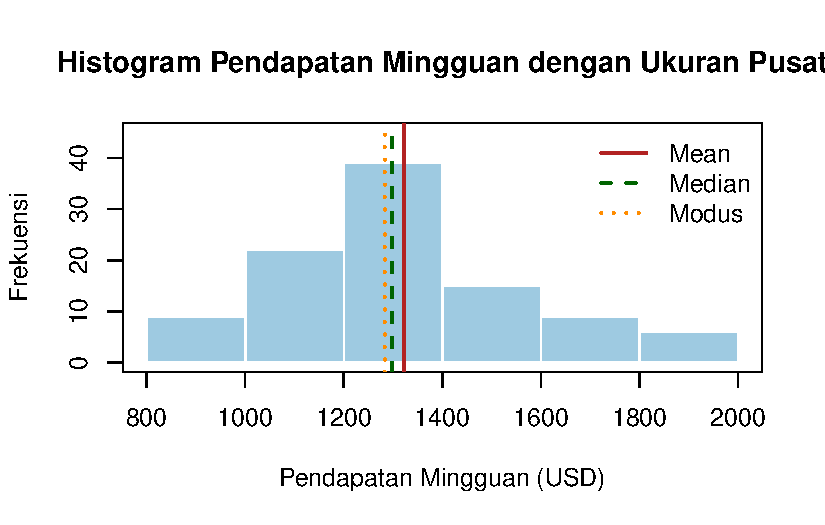
\includegraphics[keepaspectratio]{chapters/P05_files/figure-pdf/unnamed-chunk-39-1.pdf}}

\textbf{Interpretasi:} Mean (1322.5) \textgreater{} Median (1297.9)
\textgreater{} Modus (1283.4), pola khas distribusi yang
\textbf{menjulur ke kanan} (sedikit karyawan berpendapatan tinggi
menarik mean ke atas). Koefisien kemencengan Pearson-nya 0.29 (positif,
agak menceng kanan). Simpangan baku sekitar 256 USD dengan CV 19.3\%.
Pendapatan ``tipikal'' sebaiknya dilaporkan dengan median (sekitar 1298
USD).

\subsection{Seberapa Akurat Aproksimasi Data
Terkelompok?}\label{seberapa-akurat-aproksimasi-data-terkelompok}

Kita punya data mentah nilai ujian sekaligus tabel kelompoknya, sehingga
dapat membandingkan hasil \textbf{eksak} dan \textbf{aproksimasi}:

\begin{Shaded}
\begin{Highlighting}[]
\NormalTok{eksak }\OtherTok{\textless{}{-}} \FunctionTok{c}\NormalTok{(}\AttributeTok{Mean =} \FunctionTok{mean}\NormalTok{(nilai\_ujian), }\AttributeTok{Median =} \FunctionTok{median}\NormalTok{(nilai\_ujian), }\AttributeTok{SD =} \FunctionTok{sd}\NormalTok{(nilai\_ujian))}
\NormalTok{aprox }\OtherTok{\textless{}{-}} \FunctionTok{statistik\_terkelompok}\NormalTok{(batas\_nyata\_u, f\_ujian)[}\FunctionTok{c}\NormalTok{(}\StringTok{"Mean"}\NormalTok{, }\StringTok{"Median"}\NormalTok{, }\StringTok{"SD"}\NormalTok{)]}

\NormalTok{knitr}\SpecialCharTok{::}\FunctionTok{kable}\NormalTok{(}\FunctionTok{round}\NormalTok{(}\FunctionTok{rbind}\NormalTok{(}\StringTok{"Data mentah (eksak)"} \OtherTok{=}\NormalTok{ eksak, }\StringTok{"Data terkelompok (aproksimasi)"} \OtherTok{=}\NormalTok{ aprox), }\DecValTok{2}\NormalTok{),}
\AttributeTok{caption =} \StringTok{"Perbandingan Statistik Eksak vs Aproksimasi Data Terkelompok"}\NormalTok{)}
\end{Highlighting}
\end{Shaded}

\begin{longtable}[]{@{}lrrr@{}}
\caption{Perbandingan Statistik Eksak vs Aproksimasi Data
Terkelompok}\tabularnewline
\toprule\noalign{}
& Mean & Median & SD \\
\midrule\noalign{}
\endfirsthead
\toprule\noalign{}
& Mean & Median & SD \\
\midrule\noalign{}
\endhead
\bottomrule\noalign{}
\endlastfoot
Data mentah (eksak) & 80.13 & 80.5 & 9.33 \\
Data terkelompok (aproksimasi) & 80.30 & 80.5 & 9.42 \\
\end{longtable}

Selisihnya kecil, tetapi tidak nol, karena pengelompokan membuang
informasi nilai asli tiap data. \textbf{Selalu gunakan data mentah jika
tersedia}; gunakan rumus data terkelompok hanya jika data mentah tidak
ada.

\section{Etika Pelaporan: Ketika Rata-rata
Menyesatkan}\label{etika-pelaporan-ketika-rata-rata-menyesatkan}

Sama seperti grafik, ukuran statistik dapat menyesatkan -- disengaja
atau tidak -- bila dipilih atau dilaporkan secara keliru.

\subsection{Contoh 1: Rata-rata pada Data
Menceng}\label{contoh-1-rata-rata-pada-data-menceng}

\emph{``Rata-rata gaji di perusahaan kami mencapai 10,8 juta rupiah per
bulan!''} Kalimat ini benar secara perhitungan untuk data gaji, tetapi
menyesatkan: enam dari tujuh karyawan bergaji di bawah 6 juta. Untuk
data menceng atau beroutlier, laporkan \textbf{median}.

\begin{Shaded}
\begin{Highlighting}[]
\FunctionTok{c}\NormalTok{(}\AttributeTok{Mean =} \FunctionTok{mean}\NormalTok{(gaji), }\AttributeTok{Median =} \FunctionTok{median}\NormalTok{(gaji))}
\end{Highlighting}
\end{Shaded}

\begin{verbatim}
    Mean   Median 
10.82857  5.20000 
\end{verbatim}

\begin{Shaded}
\begin{Highlighting}[]
\FunctionTok{sum}\NormalTok{(gaji }\SpecialCharTok{\textless{}} \FunctionTok{mean}\NormalTok{(gaji))   }\CommentTok{\# banyaknya karyawan bergaji di bawah "rata{-}rata"}
\end{Highlighting}
\end{Shaded}

\begin{verbatim}
[1] 6
\end{verbatim}

\subsection{Contoh 2: Rata-rata dari
Rata-rata}\label{contoh-2-rata-rata-dari-rata-rata}

Kelas A (30 mahasiswa) memiliki rata-rata 80, dan Kelas B (10 mahasiswa)
memiliki rata-rata 70. Berapa rata-rata gabungan?

\begin{Shaded}
\begin{Highlighting}[]
\NormalTok{rata }\OtherTok{\textless{}{-}} \FunctionTok{c}\NormalTok{(}\AttributeTok{A =} \DecValTok{80}\NormalTok{, }\AttributeTok{B =} \DecValTok{70}\NormalTok{)}
\NormalTok{ukuran\_kelas }\OtherTok{\textless{}{-}} \FunctionTok{c}\NormalTok{(}\AttributeTok{A =} \DecValTok{30}\NormalTok{, }\AttributeTok{B =} \DecValTok{10}\NormalTok{)}

\FunctionTok{mean}\NormalTok{(rata)                              }\CommentTok{\# SALAH: mengabaikan ukuran kelas}
\end{Highlighting}
\end{Shaded}

\begin{verbatim}
[1] 75
\end{verbatim}

\begin{Shaded}
\begin{Highlighting}[]
\FunctionTok{weighted.mean}\NormalTok{(rata, }\AttributeTok{w =}\NormalTok{ ukuran\_kelas)   }\CommentTok{\# BENAR: rata{-}rata tertimbang}
\end{Highlighting}
\end{Shaded}

\begin{verbatim}
[1] 77.5
\end{verbatim}

Rata-rata sederhana (75) salah karena memperlakukan kedua kelas sama
penting; rata-rata gabungan yang benar adalah \textbf{77,5} karena Kelas
A memiliki lebih banyak mahasiswa.

\subsection{Contoh 3: Rata-rata pada Data
Bimodal}\label{contoh-3-rata-rata-pada-data-bimodal}

Pada data \texttt{data\_bimodal} (bagian Bentuk Distribusi), mean
sekitar 50, padahal hampir tidak ada data di sekitar nilai tersebut.
Mean di sini ``merata-ratakan'' dua kelompok berbeda dan tidak mewakili
siapa pun.

\subsection{Contoh 4: Pusat Tanpa
Sebaran}\label{contoh-4-pusat-tanpa-sebaran}

{\def\LTcaptype{none} % do not increment counter
\begin{longtable}[]{@{}
  >{\raggedright\arraybackslash}p{(\linewidth - 2\tabcolsep) * \real{0.5000}}
  >{\raggedright\arraybackslash}p{(\linewidth - 2\tabcolsep) * \real{0.5000}}@{}}
\toprule\noalign{}
\begin{minipage}[b]{\linewidth}\raggedright
Pelaporan sederhana
\end{minipage} & \begin{minipage}[b]{\linewidth}\raggedright
Pelaporan lebih baik
\end{minipage} \\
\midrule\noalign{}
\endhead
\bottomrule\noalign{}
\endlastfoot
``Rata-rata nilai ujian adalah 80.'' & ``Rata-rata nilai ujian 80.1 (SD
9.3; median 80.5; rentang 63--95; n = 30).'' \\
\end{longtable}
}

Pelaporan yang lebih baik memungkinkan pembaca menilai apakah
``rata-rata 80'' mewakili kelas secara wajar atau tidak.

\subsection{Daftar Periksa (Checklist) Pelaporan Statistik yang
Jujur}\label{daftar-periksa-checklist-pelaporan-statistik-yang-jujur}

\begin{itemize}
\tightlist
\item[$\square$]
  Ukuran pusat selalu disertai ukuran sebaran (mean dengan SD; median
  dengan rentang atau IQR)
\item[$\square$]
  Ukuran sesuai dengan skala pengukuran (tidak ada ``rata-rata'' untuk
  data nominal)
\item[$\square$]
  Data menceng atau beroutlier dilaporkan dengan median
\item[$\square$]
  Ukuran sampel (\(n\)) dicantumkan
\item[$\square$]
  Rata-rata gabungan memakai bobot yang tepat
\item[$\square$]
  Keputusan menghapus/mempertahankan outlier dijelaskan
\item[$\square$]
  Perbandingan variabilitas antarvariabel berbeda skala memakai
  koefisien variasi
\end{itemize}

\section{Studi Kasus Komprehensif: Membandingkan Dua
Kelas}\label{studi-kasus-komprehensif-membandingkan-dua-kelas}

\textbf{Konteks:} Dosen Statistika membandingkan nilai ujian dua kelas
paralel, masing-masing 30 mahasiswa. Kelas A adalah data
\texttt{nilai\_ujian} yang sudah kita pakai. Kelas B dicatat berikut
ini.

\begin{Shaded}
\begin{Highlighting}[]
\NormalTok{kelas\_A }\OtherTok{\textless{}{-}}\NormalTok{ nilai\_ujian}
\NormalTok{kelas\_B }\OtherTok{\textless{}{-}} \FunctionTok{c}\NormalTok{(}\DecValTok{72}\NormalTok{, }\DecValTok{96}\NormalTok{, }\DecValTok{56}\NormalTok{, }\DecValTok{85}\NormalTok{, }\DecValTok{100}\NormalTok{, }\DecValTok{64}\NormalTok{, }\DecValTok{91}\NormalTok{, }\DecValTok{54}\NormalTok{, }\DecValTok{78}\NormalTok{, }\DecValTok{93}\NormalTok{,}
\DecValTok{61}\NormalTok{, }\DecValTok{87}\NormalTok{, }\DecValTok{99}\NormalTok{, }\DecValTok{68}\NormalTok{, }\DecValTok{81}\NormalTok{, }\DecValTok{56}\NormalTok{, }\DecValTok{94}\NormalTok{, }\DecValTok{70}\NormalTok{, }\DecValTok{89}\NormalTok{, }\DecValTok{62}\NormalTok{,}
\DecValTok{97}\NormalTok{, }\DecValTok{74}\NormalTok{, }\DecValTok{83}\NormalTok{, }\DecValTok{65}\NormalTok{, }\DecValTok{92}\NormalTok{, }\DecValTok{76}\NormalTok{, }\DecValTok{98}\NormalTok{, }\DecValTok{80}\NormalTok{, }\DecValTok{84}\NormalTok{, }\DecValTok{95}\NormalTok{)}
\end{Highlighting}
\end{Shaded}

\subsection{Langkah 1: Ringkasan Statistik
Lengkap}\label{langkah-1-ringkasan-statistik-lengkap}

\begin{Shaded}
\begin{Highlighting}[]
\NormalTok{ringkasan }\OtherTok{\textless{}{-}} \ControlFlowTok{function}\NormalTok{(x) \{}
\FunctionTok{c}\NormalTok{(}\AttributeTok{n =} \FunctionTok{length}\NormalTok{(x), }\AttributeTok{Mean =} \FunctionTok{mean}\NormalTok{(x), }\AttributeTok{Median =} \FunctionTok{median}\NormalTok{(x),}
\AttributeTok{Modus =} \FunctionTok{hitung\_modus}\NormalTok{(x)[}\DecValTok{1}\NormalTok{],}
\AttributeTok{Min =} \FunctionTok{min}\NormalTok{(x), }\AttributeTok{Maks =} \FunctionTok{max}\NormalTok{(x), }\AttributeTok{Rentang =} \FunctionTok{diff}\NormalTok{(}\FunctionTok{range}\NormalTok{(x)),}
\AttributeTok{Varians =} \FunctionTok{var}\NormalTok{(x), }\AttributeTok{SD =} \FunctionTok{sd}\NormalTok{(x), }\AttributeTok{CV\_persen =} \FunctionTok{sd}\NormalTok{(x) }\SpecialCharTok{/} \FunctionTok{mean}\NormalTok{(x) }\SpecialCharTok{*} \DecValTok{100}\NormalTok{)}
\NormalTok{\}}

\NormalTok{knitr}\SpecialCharTok{::}\FunctionTok{kable}\NormalTok{(}\FunctionTok{round}\NormalTok{(}\FunctionTok{sapply}\NormalTok{(}\FunctionTok{list}\NormalTok{(}\AttributeTok{Kelas\_A =}\NormalTok{ kelas\_A, }\AttributeTok{Kelas\_B =}\NormalTok{ kelas\_B), ringkasan), }\DecValTok{2}\NormalTok{),}
\AttributeTok{caption =} \StringTok{"Ringkasan Statistik Deskriptif Kelas A dan Kelas B"}\NormalTok{)}
\end{Highlighting}
\end{Shaded}

\begin{longtable}[]{@{}lrr@{}}
\caption{Ringkasan Statistik Deskriptif Kelas A dan Kelas
B}\tabularnewline
\toprule\noalign{}
& Kelas\_A & Kelas\_B \\
\midrule\noalign{}
\endfirsthead
\toprule\noalign{}
& Kelas\_A & Kelas\_B \\
\midrule\noalign{}
\endhead
\bottomrule\noalign{}
\endlastfoot
n & 30.00 & 30.00 \\
Mean & 80.13 & 80.00 \\
Median & 80.50 & 82.00 \\
Modus & NA & 56.00 \\
Min & 63.00 & 54.00 \\
Maks & 95.00 & 100.00 \\
Rentang & 32.00 & 46.00 \\
Varians & 87.02 & 207.72 \\
SD & 9.33 & 14.41 \\
CV\_persen & 11.64 & 18.02 \\
\end{longtable}

\subsection{Langkah 2: Visualisasi
Berdampingan}\label{langkah-2-visualisasi-berdampingan}

\begin{Shaded}
\begin{Highlighting}[]
\FunctionTok{layout}\NormalTok{(}\FunctionTok{matrix}\NormalTok{(}\FunctionTok{c}\NormalTok{(}\DecValTok{1}\NormalTok{, }\DecValTok{2}\NormalTok{, }\DecValTok{3}\NormalTok{, }\DecValTok{3}\NormalTok{), }\AttributeTok{nrow =} \DecValTok{2}\NormalTok{, }\AttributeTok{byrow =} \ConstantTok{TRUE}\NormalTok{), }\AttributeTok{heights =} \FunctionTok{c}\NormalTok{(}\DecValTok{3}\NormalTok{, }\FloatTok{2.6}\NormalTok{))}

\FunctionTok{hist}\NormalTok{(kelas\_A, }\AttributeTok{breaks =} \FunctionTok{seq}\NormalTok{(}\DecValTok{50}\NormalTok{, }\DecValTok{100}\NormalTok{, }\AttributeTok{by =} \DecValTok{10}\NormalTok{), }\AttributeTok{col =} \StringTok{"steelblue"}\NormalTok{, }\AttributeTok{border =} \StringTok{"white"}\NormalTok{,}
\AttributeTok{ylim =} \FunctionTok{c}\NormalTok{(}\DecValTok{0}\NormalTok{, }\DecValTok{12}\NormalTok{), }\AttributeTok{main =} \StringTok{"Kelas A"}\NormalTok{, }\AttributeTok{xlab =} \StringTok{"Nilai"}\NormalTok{, }\AttributeTok{ylab =} \StringTok{"Frekuensi"}\NormalTok{)}
\FunctionTok{abline}\NormalTok{(}\AttributeTok{v =} \FunctionTok{mean}\NormalTok{(kelas\_A),   }\AttributeTok{col =} \StringTok{"red"}\NormalTok{,  }\AttributeTok{lwd =} \DecValTok{2}\NormalTok{)}
\FunctionTok{abline}\NormalTok{(}\AttributeTok{v =} \FunctionTok{median}\NormalTok{(kelas\_A), }\AttributeTok{col =} \StringTok{"blue"}\NormalTok{, }\AttributeTok{lwd =} \DecValTok{2}\NormalTok{, }\AttributeTok{lty =} \DecValTok{2}\NormalTok{)}

\FunctionTok{hist}\NormalTok{(kelas\_B, }\AttributeTok{breaks =} \FunctionTok{seq}\NormalTok{(}\DecValTok{50}\NormalTok{, }\DecValTok{100}\NormalTok{, }\AttributeTok{by =} \DecValTok{10}\NormalTok{), }\AttributeTok{col =} \StringTok{"darkorange"}\NormalTok{, }\AttributeTok{border =} \StringTok{"white"}\NormalTok{,}
\AttributeTok{ylim =} \FunctionTok{c}\NormalTok{(}\DecValTok{0}\NormalTok{, }\DecValTok{12}\NormalTok{), }\AttributeTok{main =} \StringTok{"Kelas B"}\NormalTok{, }\AttributeTok{xlab =} \StringTok{"Nilai"}\NormalTok{, }\AttributeTok{ylab =} \StringTok{"Frekuensi"}\NormalTok{)}
\FunctionTok{abline}\NormalTok{(}\AttributeTok{v =} \FunctionTok{mean}\NormalTok{(kelas\_B),   }\AttributeTok{col =} \StringTok{"red"}\NormalTok{,  }\AttributeTok{lwd =} \DecValTok{2}\NormalTok{)}
\FunctionTok{abline}\NormalTok{(}\AttributeTok{v =} \FunctionTok{median}\NormalTok{(kelas\_B), }\AttributeTok{col =} \StringTok{"blue"}\NormalTok{, }\AttributeTok{lwd =} \DecValTok{2}\NormalTok{, }\AttributeTok{lty =} \DecValTok{2}\NormalTok{)}
\FunctionTok{legend}\NormalTok{(}\StringTok{"topleft"}\NormalTok{, }\AttributeTok{legend =} \FunctionTok{c}\NormalTok{(}\StringTok{"Mean"}\NormalTok{, }\StringTok{"Median"}\NormalTok{), }\AttributeTok{col =} \FunctionTok{c}\NormalTok{(}\StringTok{"red"}\NormalTok{, }\StringTok{"blue"}\NormalTok{),}
\AttributeTok{lwd =} \DecValTok{2}\NormalTok{, }\AttributeTok{lty =} \FunctionTok{c}\NormalTok{(}\DecValTok{1}\NormalTok{, }\DecValTok{2}\NormalTok{), }\AttributeTok{bty =} \StringTok{"n"}\NormalTok{, }\AttributeTok{cex =} \FloatTok{0.8}\NormalTok{)}

\FunctionTok{stripchart}\NormalTok{(}\FunctionTok{list}\NormalTok{(}\StringTok{"Kelas A"} \OtherTok{=}\NormalTok{ kelas\_A, }\StringTok{"Kelas B"} \OtherTok{=}\NormalTok{ kelas\_B), }\AttributeTok{method =} \StringTok{"jitter"}\NormalTok{, }\AttributeTok{pch =} \DecValTok{16}\NormalTok{,}
\AttributeTok{col =} \FunctionTok{c}\NormalTok{(}\StringTok{"steelblue"}\NormalTok{, }\StringTok{"darkorange"}\NormalTok{), }\AttributeTok{las =} \DecValTok{1}\NormalTok{, }\AttributeTok{xlim =} \FunctionTok{c}\NormalTok{(}\DecValTok{50}\NormalTok{, }\DecValTok{100}\NormalTok{), }\AttributeTok{ylim =} \FunctionTok{c}\NormalTok{(}\FloatTok{0.6}\NormalTok{, }\FloatTok{2.6}\NormalTok{),}
\AttributeTok{xlab =} \StringTok{"Nilai"}\NormalTok{, }\AttributeTok{main =} \StringTok{"Diagram Titik Perbandingan (garis = mean +{-} 1 SD)"}\NormalTok{)}
\ControlFlowTok{for}\NormalTok{ (i }\ControlFlowTok{in} \DecValTok{1}\SpecialCharTok{:}\DecValTok{2}\NormalTok{) \{}
\NormalTok{kls }\OtherTok{\textless{}{-}} \FunctionTok{list}\NormalTok{(kelas\_A, kelas\_B)[[i]]}
\FunctionTok{segments}\NormalTok{(}\FunctionTok{mean}\NormalTok{(kls) }\SpecialCharTok{{-}} \FunctionTok{sd}\NormalTok{(kls), i }\SpecialCharTok{+} \FloatTok{0.3}\NormalTok{, }\FunctionTok{mean}\NormalTok{(kls) }\SpecialCharTok{+} \FunctionTok{sd}\NormalTok{(kls), i }\SpecialCharTok{+} \FloatTok{0.3}\NormalTok{, }\AttributeTok{lwd =} \DecValTok{3}\NormalTok{)}
\FunctionTok{points}\NormalTok{(}\FunctionTok{mean}\NormalTok{(kls), i }\SpecialCharTok{+} \FloatTok{0.3}\NormalTok{, }\AttributeTok{pch =} \DecValTok{18}\NormalTok{, }\AttributeTok{cex =} \DecValTok{2}\NormalTok{, }\AttributeTok{col =} \StringTok{"firebrick"}\NormalTok{)}
\NormalTok{\}}
\end{Highlighting}
\end{Shaded}

\pandocbounded{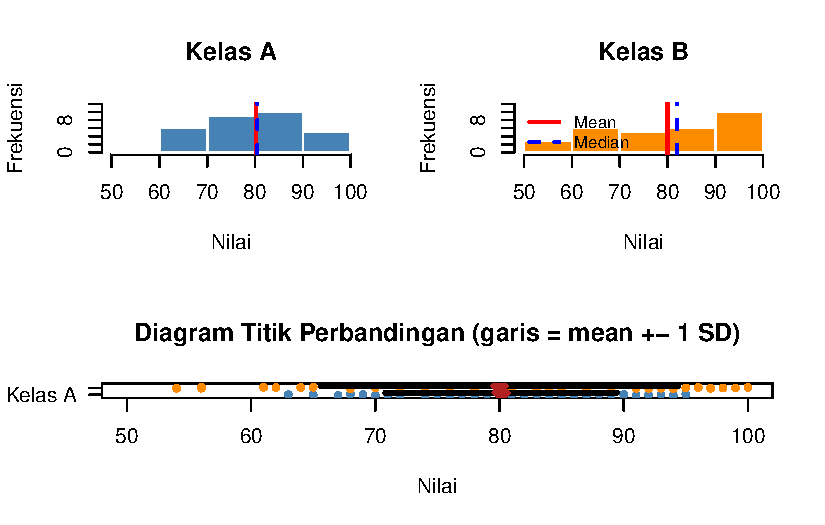
\includegraphics[keepaspectratio]{chapters/P05_files/figure-pdf/unnamed-chunk-45-1.pdf}}

\begin{Shaded}
\begin{Highlighting}[]
\FunctionTok{layout}\NormalTok{(}\DecValTok{1}\NormalTok{)}
\end{Highlighting}
\end{Shaded}

\subsection{Langkah 3: Posisi Relatif Seorang
Mahasiswa}\label{langkah-3-posisi-relatif-seorang-mahasiswa}

Seorang mahasiswa mendapat nilai \textbf{90}. Seberapa baik posisinya
jika ia berada di Kelas A dibandingkan Kelas B?

\begin{Shaded}
\begin{Highlighting}[]
\NormalTok{z\_A }\OtherTok{\textless{}{-}}\NormalTok{ (}\DecValTok{90} \SpecialCharTok{{-}} \FunctionTok{mean}\NormalTok{(kelas\_A)) }\SpecialCharTok{/} \FunctionTok{sd}\NormalTok{(kelas\_A)}
\NormalTok{z\_B }\OtherTok{\textless{}{-}}\NormalTok{ (}\DecValTok{90} \SpecialCharTok{{-}} \FunctionTok{mean}\NormalTok{(kelas\_B)) }\SpecialCharTok{/} \FunctionTok{sd}\NormalTok{(kelas\_B)}
\NormalTok{knitr}\SpecialCharTok{::}\FunctionTok{kable}\NormalTok{(}\FunctionTok{data.frame}\NormalTok{(}\AttributeTok{Kelas =} \FunctionTok{c}\NormalTok{(}\StringTok{"A"}\NormalTok{, }\StringTok{"B"}\NormalTok{),}
\AttributeTok{Mean =} \FunctionTok{round}\NormalTok{(}\FunctionTok{c}\NormalTok{(}\FunctionTok{mean}\NormalTok{(kelas\_A), }\FunctionTok{mean}\NormalTok{(kelas\_B)), }\DecValTok{2}\NormalTok{),}
\AttributeTok{SD =} \FunctionTok{round}\NormalTok{(}\FunctionTok{c}\NormalTok{(}\FunctionTok{sd}\NormalTok{(kelas\_A), }\FunctionTok{sd}\NormalTok{(kelas\_B)), }\DecValTok{2}\NormalTok{),}
\AttributeTok{z\_score =} \FunctionTok{round}\NormalTok{(}\FunctionTok{c}\NormalTok{(z\_A, z\_B), }\DecValTok{2}\NormalTok{)),}
\AttributeTok{caption =} \StringTok{"Posisi Relatif Nilai 90"}\NormalTok{)}
\end{Highlighting}
\end{Shaded}

\begin{longtable}[]{@{}lrrr@{}}
\caption{Posisi Relatif Nilai 90}\tabularnewline
\toprule\noalign{}
Kelas & Mean & SD & z\_score \\
\midrule\noalign{}
\endfirsthead
\toprule\noalign{}
Kelas & Mean & SD & z\_score \\
\midrule\noalign{}
\endhead
\bottomrule\noalign{}
\endlastfoot
A & 80.13 & 9.33 & 1.06 \\
B & 80.00 & 14.41 & 0.69 \\
\end{longtable}

\subsection{Pertanyaan Diskusi dan
Jawaban}\label{pertanyaan-diskusi-dan-jawaban-4}

\textbf{1. Kelas mana yang berprestasi lebih baik berdasarkan ukuran
pusat?}

Mean kedua kelas hampir identik (80.1 vs 80), sehingga berdasarkan mean
saja keduanya ``sama''. Namun median Kelas B (82) lebih tinggi daripada
mean-nya (80), yang mengindikasikan distribusi \textbf{menjulur kiri}:
mayoritas mahasiswa Kelas B bernilai relatif tinggi, tetapi ditarik
turun oleh segelintir nilai rendah (54--61). Kelas A hampir simetris
(mean ≈ median).

\textbf{2. Kelas mana yang lebih homogen?}

\textbf{Kelas A.} Rentangnya lebih sempit (32 vs 46), simpangan bakunya
lebih kecil (9.3 vs 14.4), dan CV-nya lebih rendah (11.6\% vs 18\%).
Kelas B jauh lebih beragam: ada mahasiswa yang sangat unggul sekaligus
yang tertinggal.

\textbf{3. Mengapa nilai 90 tampak ``lebih istimewa'' di Kelas A?}

Karena sebaran Kelas A lebih kecil, nilai 90 berada 1.06 SD di atas mean
Kelas A, tetapi hanya 0.69 SD di atas mean Kelas B. Nilai yang sama
menempati posisi relatif berbeda tergantung sebaran kelasnya.

\textbf{4. Apa rekomendasi bagi dosen?}

Kelas A cukup ditangani dengan pengajaran standar. Kelas B membutuhkan
pendekatan berlapis: pendampingan tambahan bagi kelompok bernilai
rendah, dan materi pengayaan bagi kelompok bernilai tinggi. Kesimpulan
ini tidak akan terlihat bila hanya membandingkan mean.

\section{Latihan Mandiri}\label{latihan-mandiri-4}

\subsection{Latihan Utama (Exercise 2.14 Lanjutan): Kepemilikan Kartu
Kredit}\label{latihan-utama-exercise-2.14-lanjutan-kepemilikan-kartu-kredit}

\textbf{Konteks:} Sebuah sampel acak dari 80 orang dewasa ditanya
mengenai jumlah kartu kredit yang mereka miliki. Data sudah disajikan
dalam kelas (data terkelompok):

\begin{Shaded}
\begin{Highlighting}[]
\NormalTok{kelas\_kk }\OtherTok{\textless{}{-}} \FunctionTok{c}\NormalTok{(}\StringTok{"0 to 3"}\NormalTok{, }\StringTok{"4 to 7"}\NormalTok{, }\StringTok{"8 to 11"}\NormalTok{, }\StringTok{"12 or more"}\NormalTok{)}
\NormalTok{frekuensi\_kk }\OtherTok{\textless{}{-}} \FunctionTok{c}\NormalTok{(}\DecValTok{18}\NormalTok{, }\DecValTok{26}\NormalTok{, }\DecValTok{22}\NormalTok{, }\DecValTok{14}\NormalTok{)}

\CommentTok{\# Kelas terbuka "12 or more" diasumsikan mengikuti lebar kelas yang sama}
\CommentTok{\# dengan kelas sebelumnya (w = 4), sehingga batas atasnya = 15.}
\NormalTok{batas\_bawah\_kk }\OtherTok{\textless{}{-}} \FunctionTok{c}\NormalTok{(}\DecValTok{0}\NormalTok{, }\DecValTok{4}\NormalTok{, }\DecValTok{8}\NormalTok{, }\DecValTok{12}\NormalTok{)}
\NormalTok{batas\_atas\_kk  }\OtherTok{\textless{}{-}} \FunctionTok{c}\NormalTok{(}\DecValTok{3}\NormalTok{, }\DecValTok{7}\NormalTok{, }\DecValTok{11}\NormalTok{, }\DecValTok{15}\NormalTok{)}
\NormalTok{batas\_nyata\_kk }\OtherTok{\textless{}{-}} \FunctionTok{c}\NormalTok{(}\SpecialCharTok{{-}}\FloatTok{0.5}\NormalTok{, }\FloatTok{3.5}\NormalTok{, }\FloatTok{7.5}\NormalTok{, }\FloatTok{11.5}\NormalTok{, }\FloatTok{15.5}\NormalTok{)}
\end{Highlighting}
\end{Shaded}

\subsubsection{Tugas 1: Klasifikasi variabel dan pemilihan
ukuran}\label{tugas-1-klasifikasi-variabel-dan-pemilihan-ukuran}

Variabel yang diamati adalah jumlah kartu kredit yang dimiliki. Karena
berupa hasil hitungan (bilangan bulat non-negatif) dengan nol mutlak,
variabelnya \textbf{kuantitatif diskrit berskala rasio}. Dengan skala
rasio, semua ukuran pemusatan dan penyebaran (termasuk koefisien
variasi) valid untuk dihitung.

\subsubsection{\texorpdfstring{Tugas 2: Hitung titik tengah kelas
(\(m\)) untuk interval ``4 to
7''}{Tugas 2: Hitung titik tengah kelas (m) untuk interval ``4 to 7''}}\label{tugas-2-hitung-titik-tengah-kelas-m-untuk-interval-4-to-7}

\begin{Shaded}
\begin{Highlighting}[]
\NormalTok{m\_4\_7 }\OtherTok{\textless{}{-}}\NormalTok{ (}\DecValTok{4} \SpecialCharTok{+} \DecValTok{7}\NormalTok{) }\SpecialCharTok{/} \DecValTok{2}
\NormalTok{m\_4\_7}
\end{Highlighting}
\end{Shaded}

\begin{verbatim}
[1] 5.5
\end{verbatim}

Titik tengah kelas ``4 to 7'' adalah \textbf{5.5}, diperoleh dari
\(\frac{4+7}{2}\) (sama dengan menggunakan batas nyata:
\(\frac{3{,}5 + 7{,}5}{2}\)).

\subsubsection{Tugas 3: Hitung mean, median, dan
modus}\label{tugas-3-hitung-mean-median-dan-modus}

\begin{Shaded}
\begin{Highlighting}[]
\NormalTok{hasil\_kk }\OtherTok{\textless{}{-}} \FunctionTok{statistik\_terkelompok}\NormalTok{(batas\_nyata\_kk, frekuensi\_kk)}
\FunctionTok{round}\NormalTok{(hasil\_kk[}\FunctionTok{c}\NormalTok{(}\StringTok{"n"}\NormalTok{, }\StringTok{"Mean"}\NormalTok{, }\StringTok{"Median"}\NormalTok{, }\StringTok{"Modus"}\NormalTok{)], }\DecValTok{2}\NormalTok{)}
\end{Highlighting}
\end{Shaded}

\begin{verbatim}
     n   Mean Median  Modus 
 80.00   7.10   6.88   6.17 
\end{verbatim}

Kelas median dan kelas modus keduanya adalah \textbf{``4 to 7''}
(frekuensi terbesar = 26; frekuensi kumulatif melampaui 40 di kelas
ini).

\subsubsection{Tugas 4: Hitung varians, simpangan baku, dan koefisien
variasi}\label{tugas-4-hitung-varians-simpangan-baku-dan-koefisien-variasi}

\begin{Shaded}
\begin{Highlighting}[]
\FunctionTok{round}\NormalTok{(hasil\_kk[}\FunctionTok{c}\NormalTok{(}\StringTok{"Varians"}\NormalTok{, }\StringTok{"SD"}\NormalTok{, }\StringTok{"CV\_persen"}\NormalTok{)], }\DecValTok{2}\NormalTok{)}
\end{Highlighting}
\end{Shaded}

\begin{verbatim}
  Varians        SD CV_persen 
    16.85      4.10     57.82 
\end{verbatim}

\subsubsection{Tugas 5: Interpretasikan bentuk distribusi dan
variabilitasnya}\label{tugas-5-interpretasikan-bentuk-distribusi-dan-variabilitasnya}

\begin{Shaded}
\begin{Highlighting}[]
\NormalTok{sk\_kk }\OtherTok{\textless{}{-}} \DecValTok{3} \SpecialCharTok{*}\NormalTok{ (hasil\_kk[}\StringTok{"Mean"}\NormalTok{] }\SpecialCharTok{{-}}\NormalTok{ hasil\_kk[}\StringTok{"Median"}\NormalTok{]) }\SpecialCharTok{/}\NormalTok{ hasil\_kk[}\StringTok{"SD"}\NormalTok{]}
\FunctionTok{round}\NormalTok{(sk\_kk, }\DecValTok{2}\NormalTok{)}
\end{Highlighting}
\end{Shaded}

\begin{verbatim}
Mean 
0.16 
\end{verbatim}

\begin{Shaded}
\begin{Highlighting}[]
\FunctionTok{plot}\NormalTok{(}\ConstantTok{NULL}\NormalTok{, }\AttributeTok{xlim =} \FunctionTok{c}\NormalTok{(}\SpecialCharTok{{-}}\FloatTok{0.5}\NormalTok{, }\FloatTok{15.5}\NormalTok{), }\AttributeTok{ylim =} \FunctionTok{c}\NormalTok{(}\DecValTok{0}\NormalTok{, }\DecValTok{30}\NormalTok{),}
\AttributeTok{xlab =} \StringTok{"Jumlah Kartu Kredit"}\NormalTok{, }\AttributeTok{ylab =} \StringTok{"Frekuensi (f)"}\NormalTok{,}
\AttributeTok{main =} \StringTok{"Distribusi Kepemilikan Kartu Kredit (n = 80)"}\NormalTok{)}
\FunctionTok{rect}\NormalTok{(}\FunctionTok{head}\NormalTok{(batas\_nyata\_kk, }\SpecialCharTok{{-}}\DecValTok{1}\NormalTok{), }\DecValTok{0}\NormalTok{, }\FunctionTok{tail}\NormalTok{(batas\_nyata\_kk, }\SpecialCharTok{{-}}\DecValTok{1}\NormalTok{), frekuensi\_kk,}
\AttributeTok{col =} \StringTok{"\#6C5B7B"}\NormalTok{, }\AttributeTok{border =} \StringTok{"white"}\NormalTok{)}
\FunctionTok{abline}\NormalTok{(}\AttributeTok{v =}\NormalTok{ hasil\_kk[}\StringTok{"Mean"}\NormalTok{],   }\AttributeTok{col =} \StringTok{"firebrick"}\NormalTok{, }\AttributeTok{lwd =} \DecValTok{2}\NormalTok{)}
\FunctionTok{abline}\NormalTok{(}\AttributeTok{v =}\NormalTok{ hasil\_kk[}\StringTok{"Median"}\NormalTok{], }\AttributeTok{col =} \StringTok{"darkgreen"}\NormalTok{, }\AttributeTok{lwd =} \DecValTok{2}\NormalTok{, }\AttributeTok{lty =} \DecValTok{2}\NormalTok{)}
\FunctionTok{legend}\NormalTok{(}\StringTok{"topright"}\NormalTok{, }\AttributeTok{legend =} \FunctionTok{c}\NormalTok{(}\StringTok{"Mean"}\NormalTok{, }\StringTok{"Median"}\NormalTok{), }\AttributeTok{col =} \FunctionTok{c}\NormalTok{(}\StringTok{"firebrick"}\NormalTok{, }\StringTok{"darkgreen"}\NormalTok{),}
\AttributeTok{lwd =} \DecValTok{2}\NormalTok{, }\AttributeTok{lty =} \FunctionTok{c}\NormalTok{(}\DecValTok{1}\NormalTok{, }\DecValTok{2}\NormalTok{), }\AttributeTok{bty =} \StringTok{"n"}\NormalTok{)}
\end{Highlighting}
\end{Shaded}

\pandocbounded{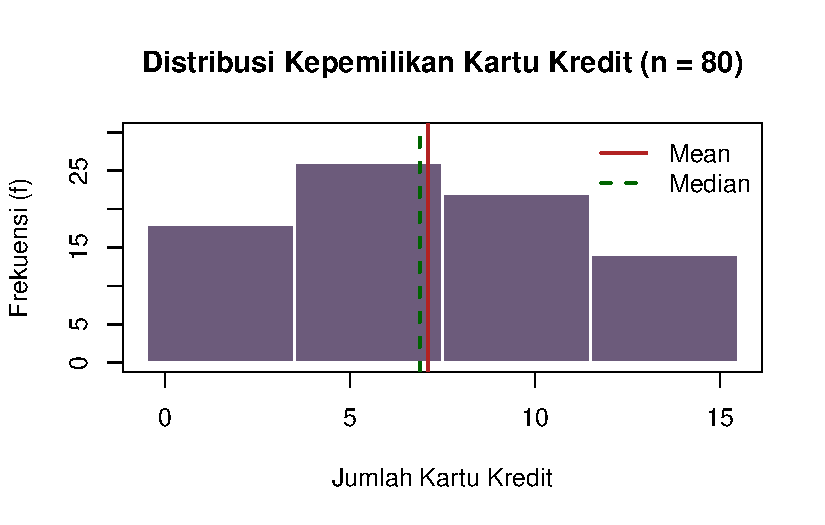
\includegraphics[keepaspectratio]{chapters/P05_files/figure-pdf/unnamed-chunk-52-1.pdf}}

\textbf{Jawaban:} Mean (7.1) sedikit di atas median (6.88) dan modus
(6.17), dengan \(Sk = 0.16\), sehingga distribusinya \textbf{hampir
simetris dengan sedikit kemencengan ke kanan}. Rata-rata orang dalam
sampel memiliki sekitar 7 kartu kredit. CV sebesar 57.8\% menunjukkan
variabilitas yang \textbf{tinggi} (simpangan baku mencapai lebih dari
separuh mean-nya) -- kepemilikan kartu kredit sangat beragam
antarindividu.

\subsubsection{Tugas 6 (Tantangan): Sensitivitas terhadap Kelas
Terbuka}\label{tugas-6-tantangan-sensitivitas-terhadap-kelas-terbuka}

Bagaimana jika kelas ``12 or more'' ternyata mencakup orang dengan
hingga 19 kartu (batas atas 19, bukan 15)?

\begin{Shaded}
\begin{Highlighting}[]
\NormalTok{batas\_nyata\_kk\_alt }\OtherTok{\textless{}{-}} \FunctionTok{c}\NormalTok{(}\SpecialCharTok{{-}}\FloatTok{0.5}\NormalTok{, }\FloatTok{3.5}\NormalTok{, }\FloatTok{7.5}\NormalTok{, }\FloatTok{11.5}\NormalTok{, }\FloatTok{19.5}\NormalTok{)   }\CommentTok{\# batas atas kelas terakhir diperlebar}

\NormalTok{sensitivitas }\OtherTok{\textless{}{-}} \FunctionTok{rbind}\NormalTok{(}
\StringTok{"Asumsi batas atas 15"} \OtherTok{=} \FunctionTok{statistik\_terkelompok}\NormalTok{(batas\_nyata\_kk, frekuensi\_kk),}
\StringTok{"Asumsi batas atas 19"} \OtherTok{=} \FunctionTok{statistik\_terkelompok}\NormalTok{(batas\_nyata\_kk\_alt, frekuensi\_kk)}
\NormalTok{)}
\NormalTok{knitr}\SpecialCharTok{::}\FunctionTok{kable}\NormalTok{(}\FunctionTok{round}\NormalTok{(sensitivitas[, }\FunctionTok{c}\NormalTok{(}\StringTok{"Mean"}\NormalTok{, }\StringTok{"Median"}\NormalTok{, }\StringTok{"Modus"}\NormalTok{, }\StringTok{"SD"}\NormalTok{)], }\DecValTok{2}\NormalTok{),}
\AttributeTok{caption =} \StringTok{"Dampak Asumsi Kelas Terbuka"}\NormalTok{)}
\end{Highlighting}
\end{Shaded}

\begin{longtable}[]{@{}lrrrr@{}}
\caption{Dampak Asumsi Kelas Terbuka}\tabularnewline
\toprule\noalign{}
& Mean & Median & Modus & SD \\
\midrule\noalign{}
\endfirsthead
\toprule\noalign{}
& Mean & Median & Modus & SD \\
\midrule\noalign{}
\endhead
\bottomrule\noalign{}
\endlastfoot
Asumsi batas atas 15 & 7.10 & 6.88 & 6.17 & 4.10 \\
Asumsi batas atas 19 & 7.45 & 6.88 & 6.17 & 4.69 \\
\end{longtable}

\textbf{Jawaban:} Median dan modus \textbf{tidak berubah} (keduanya
berada di kelas ``4 to 7''), tetapi mean dan simpangan baku
\textbf{meningkat} karena titik tengah kelas terakhir bergeser. Ini
contoh nyata bahwa median dan modus lebih tahan terhadap ketidakjelasan
kelas terbuka dibanding mean. Karena itu, asumsi batas kelas terbuka
harus selalu dinyatakan secara eksplisit.

\subsection{Latihan Tambahan
(Self-Check)}\label{latihan-tambahan-self-check-4}

Kerjakan soal-soal berikut secara mandiri sebelum melihat kunci jawaban
pada komentar kode.

\textbf{Soal A.} Data waktu tempuh (menit) 12 karyawan menuju kantor:
15, 22, 18, 30, 25, 20, 35, 28, 19, 24, 27, 33. Hitung mean, median,
modus, rentang, varians, simpangan baku, dan koefisien variasi. Waktu
tempuh berapa yang memiliki z-score terbesar?

\begin{Shaded}
\begin{Highlighting}[]
\CommentTok{\# Kerjakan di sini:}
\NormalTok{waktu }\OtherTok{\textless{}{-}} \FunctionTok{c}\NormalTok{(}\DecValTok{15}\NormalTok{, }\DecValTok{22}\NormalTok{, }\DecValTok{18}\NormalTok{, }\DecValTok{30}\NormalTok{, }\DecValTok{25}\NormalTok{, }\DecValTok{20}\NormalTok{, }\DecValTok{35}\NormalTok{, }\DecValTok{28}\NormalTok{, }\DecValTok{19}\NormalTok{, }\DecValTok{24}\NormalTok{, }\DecValTok{27}\NormalTok{, }\DecValTok{33}\NormalTok{)}
\CommentTok{\# ...}

\CommentTok{\# Kunci jawaban (jalankan setelah mencoba sendiri):}
\CommentTok{\# Mean = 24.67; Median = 24.5; Modus = tidak ada (semua nilai unik)}
\CommentTok{\# Rentang = 35 {-} 15 = 20}
\CommentTok{\# Varians = 38.24; SD = 6.18; CV = 6.18 / 24.67 x 100\% = 25.07\%}
\CommentTok{\# z{-}score terbesar (mutlak): 35 menit {-}\textgreater{} (35 {-} 24.67) / 6.18 = 1.67}
\CommentTok{\# (15 menit: z = {-}1.56). Semua data berada dalam 2 SD dari mean.}
\end{Highlighting}
\end{Shaded}

\textbf{Soal B.} Dua reksa dana memiliki statistik imbal hasil tahunan
berikut: Reksa Dana X (mean 12\%, SD 3\%) dan Reksa Dana Y (mean 25\%,
SD 5\%). Manakah yang risikonya (variabilitas) \textbf{relatif} lebih
kecil?

\begin{Shaded}
\begin{Highlighting}[]
\CommentTok{\# Kerjakan di sini:}
\CommentTok{\# cv\_x \textless{}{-} ...}
\CommentTok{\# cv\_y \textless{}{-} ...}

\CommentTok{\# Kunci jawaban:}
\CommentTok{\# CV\_X = 3 / 12 x 100\% = 25\%}
\CommentTok{\# CV\_Y = 5 / 25 x 100\% = 20\%}
\CommentTok{\# Reksa Dana Y lebih stabil secara relatif (CV lebih kecil), meskipun SD{-}nya (5\%) lebih besar.}
\end{Highlighting}
\end{Shaded}

\textbf{Soal C.} Harga (miliar rupiah) 8 rumah di suatu perumahan: 0,85;
0,90; 0,95; 0,90; 1,05; 1,10; 0,98; 9,5. (a) Hitung mean, median, dan
simpangan baku. (b) Hitung ulang ketiganya tanpa rumah termahal. (c)
Ukuran pusat mana yang sebaiknya dilaporkan? Mengapa?

\begin{Shaded}
\begin{Highlighting}[]
\CommentTok{\# Kerjakan di sini:}
\NormalTok{harga }\OtherTok{\textless{}{-}} \FunctionTok{c}\NormalTok{(}\FloatTok{0.85}\NormalTok{, }\FloatTok{0.90}\NormalTok{, }\FloatTok{0.95}\NormalTok{, }\FloatTok{0.90}\NormalTok{, }\FloatTok{1.05}\NormalTok{, }\FloatTok{1.10}\NormalTok{, }\FloatTok{0.98}\NormalTok{, }\FloatTok{9.5}\NormalTok{)}
\CommentTok{\# ...}

\CommentTok{\# Kunci jawaban:}
\CommentTok{\# (a) Mean = 2.03; Median = 0.965; SD = 3.02}
\CommentTok{\# (b) Tanpa 9.5: Mean = 0.961; Median = 0.95; SD = 0.089}
\CommentTok{\#     {-}\textgreater{} mean turun lebih dari separuh dan SD menyusut drastis; median nyaris tidak berubah.}
\CommentTok{\# (c) Laporkan MEDIAN (0.965 miliar), karena satu rumah mewah (9.5 miliar)}
\CommentTok{\#     menggeser mean ke 2.03 miliar {-}{-} dua kali lipat harga hampir semua rumah lainnya.}
\CommentTok{\# Modus = 0.90 (muncul dua kali).}
\end{Highlighting}
\end{Shaded}

\textbf{Soal D.} Rina mendapat nilai 72 pada ujian yang mean-nya 65
dengan SD 5. Dewi mendapat nilai 80 pada ujian lain yang mean-nya 70
dengan SD 10. Siapa yang prestasi relatifnya lebih baik?

\begin{Shaded}
\begin{Highlighting}[]
\CommentTok{\# Kerjakan di sini:}
\CommentTok{\# z\_rina \textless{}{-} ...}
\CommentTok{\# z\_dewi \textless{}{-} ...}

\CommentTok{\# Kunci jawaban:}
\CommentTok{\# z\_Rina = (72 {-} 65) / 5 = 1.4}
\CommentTok{\# z\_Dewi = (80 {-} 70) / 10 = 1.0}
\CommentTok{\# Rina lebih unggul secara relatif (1.4 SD di atas mean vs 1.0 SD), walaupun nilai mentah Dewi lebih tinggi.}
\end{Highlighting}
\end{Shaded}

\section{Kesalahan Umum dalam Ukuran Pemusatan dan
Penyebaran}\label{kesalahan-umum-dalam-ukuran-pemusatan-dan-penyebaran}

Ringkasan kesalahan yang paling sering dijumpai, berdasarkan
contoh-contoh pada praktikum ini:

\begin{enumerate}
\def\labelenumi{\arabic{enumi}.}
\tightlist
\item
  \textbf{Memakai mean untuk data menceng atau beroutlier} tanpa
  memeriksa median -- hasilnya tidak mewakili ``kebanyakan'' data
  (contoh: gaji, harga rumah).
\item
  \textbf{Menghitung mean untuk data nominal atau ordinal} -- misalnya
  ``rata-rata jenis kelamin'' atau merata-ratakan peringkat kepuasan
  seolah jaraknya sama.
\item
  \textbf{Lupa bahwa \texttt{var()} dan \texttt{sd()} di R memakai
  pembagi \(n-1\)} -- untuk data populasi, hasilnya sedikit berbeda dari
  \(\sigma^2\) dan \(\sigma\).
\item
  \textbf{Menyangka \texttt{range()} di R mengembalikan selisih} --
  fungsi itu mengembalikan nilai minimum dan maksimum; gunakan
  \texttt{diff(range(x))}.
\item
  \textbf{Membandingkan simpangan baku antarvariabel berbeda skala} (cm
  vs kg) tanpa koefisien variasi.
\item
  \textbf{Menggunakan koefisien variasi pada skala interval} (misalnya
  suhu °C) atau pada data dengan mean mendekati nol.
\item
  \textbf{Merata-ratakan rata-rata tanpa bobot} -- rata-rata gabungan
  harus tertimbang menurut ukuran kelompok.
\item
  \textbf{Melaporkan ukuran pusat tanpa ukuran sebaran (dan tanpa
  \(n\))} -- pembaca tidak bisa menilai keterwakilan pusat data.
\item
  \textbf{Menghapus outlier otomatis} tanpa menyelidiki penyebabnya.
\item
  \textbf{Menerapkan aturan empiris pada distribusi yang tidak berbentuk
  lonceng} -- gunakan Chebyshev untuk bentuk sembarang.
\item
  \textbf{Menganggap hasil data terkelompok sebagai nilai eksak} -- itu
  hanya aproksimasi, dan hasilnya (terutama mean dan SD) sensitif
  terhadap asumsi kelas terbuka.
\item
  \textbf{Mencari modus pada data kontinu mentah} -- nilai hampir tidak
  pernah berulang; kelompokkan dahulu dan gunakan kelas modus.
\end{enumerate}

\section{Cheat Sheet: Fungsi R yang
Digunakan}\label{cheat-sheet-fungsi-r-yang-digunakan-4}

{\def\LTcaptype{none} % do not increment counter
\begin{longtable}[]{@{}
  >{\raggedright\arraybackslash}p{(\linewidth - 2\tabcolsep) * \real{0.5000}}
  >{\raggedright\arraybackslash}p{(\linewidth - 2\tabcolsep) * \real{0.5000}}@{}}
\toprule\noalign{}
\begin{minipage}[b]{\linewidth}\raggedright
Fungsi
\end{minipage} & \begin{minipage}[b]{\linewidth}\raggedright
Kegunaan
\end{minipage} \\
\midrule\noalign{}
\endhead
\bottomrule\noalign{}
\endlastfoot
\texttt{mean(x)} & Rata-rata hitung; \texttt{mean(x,\ trim\ =\ 0.1)}
untuk trimmed mean \\
\texttt{weighted.mean(x,\ w)} & Rata-rata tertimbang dengan bobot
\texttt{w} \\
\texttt{median(x)} & Median \\
\texttt{table(x)} & Menghitung frekuensi tiap nilai (dasar mencari
modus) \\
\texttt{which.max(f)} & Indeks nilai terbesar (mencari kelas modus) \\
\texttt{summary(x)} & Min, Q1, median, mean, Q3, maks \\
\texttt{range(x)} & Nilai minimum dan maksimum (\textbf{bukan}
selisih) \\
\texttt{diff(range(x))} & Rentang \\
\texttt{var(x)} & Varians sampel (pembagi \(n-1\)) \\
\texttt{sd(x)} & Simpangan baku sampel \\
\texttt{scale(x)} & Menghitung z-score \\
\texttt{hist(x,\ breaks\ =\ ...)} & Histogram \\
\texttt{stripchart(x,\ method\ =\ ...)} & Diagram titik untuk data
kecil \\
\texttt{abline(v\ =\ ...)} & Menambahkan garis vertikal (mean, median,
dst.) pada grafik \\
\texttt{cumsum(x)} & Frekuensi kumulatif (mencari kelas median) \\
\texttt{cut(x,\ breaks\ =\ ...)} & Mengelompokkan data numerik ke dalam
kelas \\
\texttt{sapply(list,\ fungsi)} & Menerapkan fungsi ke beberapa dataset
sekaligus \\
\texttt{layout()} / \texttt{par(mfrow\ =\ ...)} & Mengatur beberapa
grafik dalam satu tampilan \\
\texttt{kable(df)} & Menampilkan data.frame sebagai tabel rapi (paket
\texttt{knitr}) \\
\end{longtable}
}

\section{Glosarium Istilah}\label{glosarium-istilah-4}

{\def\LTcaptype{none} % do not increment counter
\begin{longtable}[]{@{}
  >{\raggedright\arraybackslash}p{(\linewidth - 2\tabcolsep) * \real{0.5000}}
  >{\raggedright\arraybackslash}p{(\linewidth - 2\tabcolsep) * \real{0.5000}}@{}}
\toprule\noalign{}
\begin{minipage}[b]{\linewidth}\raggedright
Istilah
\end{minipage} & \begin{minipage}[b]{\linewidth}\raggedright
Definisi Singkat
\end{minipage} \\
\midrule\noalign{}
\endhead
\bottomrule\noalign{}
\endlastfoot
Ukuran Pemusatan & Nilai tunggal yang menggambarkan ``pusat'' atau nilai
tipikal data \\
Mean & Jumlah semua nilai dibagi banyaknya data \\
Rata-rata Tertimbang & Mean dengan bobot berbeda untuk tiap nilai \\
Trimmed Mean & Mean setelah membuang persentase tertentu data terkecil
dan terbesar \\
Median & Nilai tengah data terurut; membagi data menjadi dua bagian sama
banyak \\
Modus & Nilai yang paling sering muncul \\
Ukuran Penyebaran & Ukuran seberapa jauh data menyebar dari pusatnya \\
Rentang (Range) & Selisih nilai terbesar dan terkecil \\
Deviasi & Selisih sebuah nilai dengan mean: \(x_i - \bar{x}\) \\
Varians & Rata-rata kuadrat deviasi (pembagi \(n-1\) untuk sampel) \\
Simpangan Baku & Akar varians; ukuran sebaran dengan satuan sama seperti
data \\
Koefisien Variasi (CV) & Simpangan baku relatif terhadap mean, dalam
persen \\
Derajat Bebas & Banyaknya nilai yang bebas bervariasi; pada varians
sampel sebesar \(n-1\) \\
Skewness (Kemencengan) & Ukuran ketidaksimetrisan suatu distribusi \\
Bimodal & Distribusi dengan dua puncak (modus) berbeda \\
Outlier & Data yang nilainya jauh menyimpang dari mayoritas data \\
Robust (Tahan) & Ukuran yang tidak banyak berubah oleh keberadaan
outlier \\
Z-Score & Jarak sebuah nilai dari mean dalam satuan simpangan baku \\
Aturan Empiris & Aturan 68-95-99,7 untuk data berbentuk lonceng \\
Teorema Chebyshev & Batas minimal proporsi data dalam \(k\) simpangan
baku, berlaku untuk sembarang distribusi \\
Titik Tengah Kelas (\(m\)) & Nilai representatif kelas pada perhitungan
data terkelompok \\
Kelas Median / Kelas Modus & Kelas yang memuat median / kelas dengan
frekuensi terbesar \\
\end{longtable}
}

\section{Rangkuman dan Kesimpulan}\label{rangkuman-dan-kesimpulan-4}

\begin{enumerate}
\def\labelenumi{\arabic{enumi}.}
\tightlist
\item
  \textbf{Pusat dan sebaran berpasangan.} Ukuran pemusatan menjawab ``di
  mana pusat data?'', ukuran penyebaran menjawab ``seberapa menyebar?''.
  Melaporkan salah satunya saja tidak lengkap.
\item
  \textbf{Skala data menentukan ukuran yang valid.} Modus untuk nominal;
  median untuk ordinal; mean untuk interval/rasio; koefisien variasi
  khusus rasio.
\item
  \textbf{Mean vs median.} Mean memakai seluruh data tetapi sensitif
  terhadap outlier; median tahan outlier. Selisih keduanya menandakan
  kemencengan: mean \textgreater{} median (menjulur kanan), mean
  \textless{} median (menjulur kiri).
\item
  \textbf{Varians dan simpangan baku} mengukur rata-rata jarak data dari
  mean. Untuk sampel, pembaginya \(n-1\). Simpangan baku berpasangan
  dengan mean.
\item
  \textbf{Koefisien variasi dan z-score} memungkinkan perbandingan yang
  adil lintas skala: CV untuk variabilitas, z-score untuk posisi relatif
  individu.
\item
  \textbf{Nilai ekstrem} menarik mean, SD, rentang, dan CV, tetapi
  hampir tidak memengaruhi median. Nilai ekstrem harus diselidiki, bukan
  dibuang otomatis.
\item
  \textbf{Data terkelompok memberi aproksimasi.} Rumus titik tengah,
  kelas median, dan kelas modus berguna ketika data mentah tidak
  tersedia, tetapi hasilnya tidak eksak.
\item
  \textbf{Pelaporan yang jujur} mencantumkan ukuran pusat, sebaran, dan
  ukuran sampel, serta memilih ukuran yang sesuai dengan bentuk data.
\end{enumerate}

\textbf{Jembatan ke sesi berikutnya:} ukuran pusat dan sebaran meringkas
data dengan dua angka, tetapi menyembunyikan detail seperti ``di mana
25\% data terbawah?'' atau ``nilai mana yang terlalu jauh?''. Pertemuan
6 membahas ukuran posisi (kuartil, desil, persentil), IQR dan boxplot,
bentuk distribusi, serta deteksi dan penanganan outlier secara formal.

\section{Referensi Pendukung}\label{referensi-pendukung-4}

Materi ini merangkum topik ukuran pemusatan dan penyebaran data
(\emph{measures of central tendency and dispersion}) yang umum dibahas
pada bab statistika deskriptif buku teks pengantar statistika
bisnis/data science. Mahasiswa disarankan melengkapi pemahaman dengan
merujuk pada:

\begin{itemize}
\tightlist
\item
  Modul/slide perkuliahan ``Introduction to Statistics (SDT-1102)'' --
  Pertemuan 5: Statistika Deskriptif (\emph{Measures of Central Tendency
  and Dispersion}).
\item
  Dokumentasi resmi R: \texttt{?mean}, \texttt{?median}, \texttt{?var},
  \texttt{?sd}, \texttt{?weighted.mean}, \texttt{?scale} (dapat diakses
  langsung di R/RStudio).
\item
  Buku teks pengantar statistika deskriptif pada bab Ukuran Pemusatan
  dan Ukuran Penyebaran.
\end{itemize}

\bookmarksetup{startatroot}

\chapter{Sampling Distribution}\label{sampling-distribution}

\section{Tiga Distribusi yang Harus
Dibedakan}\label{tiga-distribusi-yang-harus-dibedakan}

{\def\LTcaptype{none} % do not increment counter
\begin{longtable}[]{@{}
  >{\raggedright\arraybackslash}p{(\linewidth - 6\tabcolsep) * \real{0.2500}}
  >{\raggedright\arraybackslash}p{(\linewidth - 6\tabcolsep) * \real{0.2500}}
  >{\raggedright\arraybackslash}p{(\linewidth - 6\tabcolsep) * \real{0.2500}}
  >{\raggedright\arraybackslash}p{(\linewidth - 6\tabcolsep) * \real{0.2500}}@{}}
\toprule\noalign{}
\begin{minipage}[b]{\linewidth}\raggedright
Distribusi
\end{minipage} & \begin{minipage}[b]{\linewidth}\raggedright
Isinya
\end{minipage} & \begin{minipage}[b]{\linewidth}\raggedright
Jumlah nilai
\end{minipage} & \begin{minipage}[b]{\linewidth}\raggedright
Contoh
\end{minipage} \\
\midrule\noalign{}
\endhead
\bottomrule\noalign{}
\endlastfoot
\textbf{Distribusi populasi} & Nilai setiap unit populasi & \(N\) &
Pengeluaran 20.000 mahasiswa \\
\textbf{Distribusi sampel} & Nilai unit dalam satu sampel & \(n\) &
Pengeluaran 40 mahasiswa yang disurvei \\
\textbf{Distribusi sampling} & Nilai statistik (misalnya \(\bar{x}\))
dari banyak sampel & Sebanyak sampel yang (dibayangkan) diambil &
\(\bar{x}\) dari 10.000 sampel berukuran 40 \\
\end{longtable}
}

Distribusi sampling adalah konsep teoretis: dalam praktik kita hanya
memiliki satu sampel. Namun dengan simulasi kita dapat ``melihatnya''.

\subsection{Populasi Simulasi}\label{populasi-simulasi-1}

Kita memakai populasi 20.000 mahasiswa dengan variabel waktu layar
harian (jam) yang menjulur kanan --- bentuk yang sengaja dipilih jauh
dari lonceng.

\begin{Shaded}
\begin{Highlighting}[]
\FunctionTok{set.seed}\NormalTok{(}\DecValTok{909}\NormalTok{)}
\NormalTok{N }\OtherTok{\textless{}{-}} \DecValTok{20000}
\NormalTok{populasi }\OtherTok{\textless{}{-}} \FunctionTok{round}\NormalTok{(}\FunctionTok{rgamma}\NormalTok{(N, }\AttributeTok{shape =} \DecValTok{2}\NormalTok{, }\AttributeTok{rate =} \FloatTok{0.4}\NormalTok{), }\DecValTok{2}\NormalTok{) }\CommentTok{\# jam per hari}
\NormalTok{mu }\OtherTok{\textless{}{-}} \FunctionTok{mean}\NormalTok{(populasi)}
\NormalTok{sigma }\OtherTok{\textless{}{-}} \FunctionTok{sqrt}\NormalTok{(}\FunctionTok{mean}\NormalTok{((populasi }\SpecialCharTok{{-}}\NormalTok{ mu)}\SpecialCharTok{\^{}}\DecValTok{2}\NormalTok{)) }\CommentTok{\# SD populasi (pembagi N)}

\FunctionTok{c}\NormalTok{(}\AttributeTok{N =}\NormalTok{ N, }\AttributeTok{mu =} \FunctionTok{round}\NormalTok{(mu, }\DecValTok{3}\NormalTok{), }\AttributeTok{sigma =} \FunctionTok{round}\NormalTok{(sigma, }\DecValTok{3}\NormalTok{))}
\end{Highlighting}
\end{Shaded}

\begin{verbatim}
        N        mu     sigma 
20000.000     5.010     3.551 
\end{verbatim}

\begin{Shaded}
\begin{Highlighting}[]
\FunctionTok{set.seed}\NormalTok{(}\DecValTok{1}\NormalTok{)}
\NormalTok{satu\_sampel }\OtherTok{\textless{}{-}} \FunctionTok{sample}\NormalTok{(populasi, }\DecValTok{40}\NormalTok{)}
\NormalTok{banyak\_rata }\OtherTok{\textless{}{-}} \FunctionTok{replicate}\NormalTok{(}\DecValTok{10000}\NormalTok{, }\FunctionTok{mean}\NormalTok{(}\FunctionTok{sample}\NormalTok{(populasi, }\DecValTok{40}\NormalTok{)))}

\FunctionTok{par}\NormalTok{(}\AttributeTok{mfrow =} \FunctionTok{c}\NormalTok{(}\DecValTok{1}\NormalTok{, }\DecValTok{3}\NormalTok{))}
\FunctionTok{hist}\NormalTok{(populasi, }\AttributeTok{breaks =} \DecValTok{40}\NormalTok{, }\AttributeTok{col =} \StringTok{"\#9ecae1"}\NormalTok{, }\AttributeTok{border =} \StringTok{"white"}\NormalTok{,}
     \AttributeTok{main =} \StringTok{"Populasi (N = 20.000)"}\NormalTok{, }\AttributeTok{xlab =} \StringTok{"Jam per hari"}\NormalTok{, }\AttributeTok{xlim =} \FunctionTok{c}\NormalTok{(}\DecValTok{0}\NormalTok{, }\DecValTok{20}\NormalTok{))}
\FunctionTok{hist}\NormalTok{(satu\_sampel, }\AttributeTok{breaks =} \DecValTok{12}\NormalTok{, }\AttributeTok{col =} \StringTok{"\#fdae6b"}\NormalTok{, }\AttributeTok{border =} \StringTok{"white"}\NormalTok{,}
     \AttributeTok{main =} \StringTok{"Satu sampel (n = 40)"}\NormalTok{, }\AttributeTok{xlab =} \StringTok{"Jam per hari"}\NormalTok{, }\AttributeTok{xlim =} \FunctionTok{c}\NormalTok{(}\DecValTok{0}\NormalTok{, }\DecValTok{20}\NormalTok{))}
\FunctionTok{hist}\NormalTok{(banyak\_rata, }\AttributeTok{breaks =} \DecValTok{40}\NormalTok{, }\AttributeTok{col =} \StringTok{"\#a1d99b"}\NormalTok{, }\AttributeTok{border =} \StringTok{"white"}\NormalTok{,}
     \AttributeTok{main =} \StringTok{"Sampling distribution x{-}bar"}\NormalTok{, }\AttributeTok{xlab =} \StringTok{"Rata{-}rata sampel (n = 40)"}\NormalTok{)}
\end{Highlighting}
\end{Shaded}

\pandocbounded{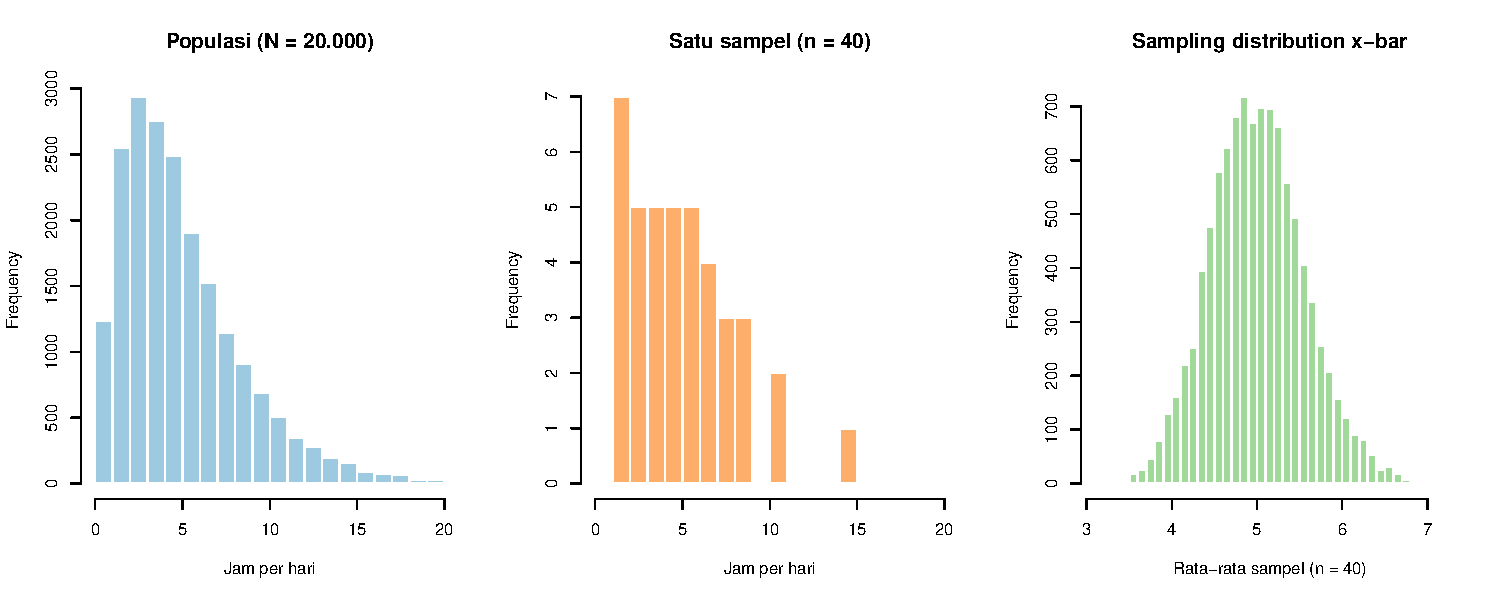
\includegraphics[keepaspectratio]{chapters/P09_files/figure-pdf/unnamed-chunk-2-1.pdf}}

\begin{Shaded}
\begin{Highlighting}[]
\FunctionTok{par}\NormalTok{(}\AttributeTok{mfrow =} \FunctionTok{c}\NormalTok{(}\DecValTok{1}\NormalTok{, }\DecValTok{1}\NormalTok{))}
\end{Highlighting}
\end{Shaded}

Populasi dan satu sampel sama-sama menjulur kanan, tetapi distribusi
rata-rata sampel jauh lebih sempit dan hampir berbentuk lonceng. Inilah
inti pertemuan ini.

\section{Distribusi Sampling Rata-rata
Sampel}\label{distribusi-sampling-rata-rata-sampel}

Untuk sampel acak berukuran \(n\) dari populasi dengan mean \(\mu\) dan
simpangan baku \(\sigma\):

{\def\LTcaptype{none} % do not increment counter
\begin{longtable}[]{@{}
  >{\raggedright\arraybackslash}p{(\linewidth - 4\tabcolsep) * \real{0.3333}}
  >{\raggedright\arraybackslash}p{(\linewidth - 4\tabcolsep) * \real{0.3333}}
  >{\raggedright\arraybackslash}p{(\linewidth - 4\tabcolsep) * \real{0.3333}}@{}}
\toprule\noalign{}
\begin{minipage}[b]{\linewidth}\raggedright
Sifat
\end{minipage} & \begin{minipage}[b]{\linewidth}\raggedright
Rumus
\end{minipage} & \begin{minipage}[b]{\linewidth}\raggedright
Arti
\end{minipage} \\
\midrule\noalign{}
\endhead
\bottomrule\noalign{}
\endlastfoot
\textbf{Mean} & \(\mu_{\bar{x}} = \mu\) & \(\bar{x}\) adalah penaksir
tak bias: rata-ratanya tepat di parameter \\
\textbf{Standard error} & \(\sigma_{\bar{x}} = \frac{\sigma}{\sqrt{n}}\)
& Sebaran \(\bar{x}\) mengecil seiring bertambahnya \(n\) \\
\textbf{Bentuk} & Normal jika populasi normal; mendekati normal untuk
\(n\) cukup besar (CLT) & Memungkinkan perhitungan peluang \\
\end{longtable}
}

\begin{Shaded}
\begin{Highlighting}[]
\NormalTok{knitr}\SpecialCharTok{::}\FunctionTok{kable}\NormalTok{(}\FunctionTok{data.frame}\NormalTok{(}
  \AttributeTok{Besaran =} \FunctionTok{c}\NormalTok{(}\StringTok{"Mean distribusi sampling"}\NormalTok{, }\StringTok{"SD distribusi sampling (SE)"}\NormalTok{),}
  \AttributeTok{Teori =} \FunctionTok{round}\NormalTok{(}\FunctionTok{c}\NormalTok{(mu, sigma }\SpecialCharTok{/} \FunctionTok{sqrt}\NormalTok{(}\DecValTok{40}\NormalTok{)), }\DecValTok{4}\NormalTok{),}
  \AttributeTok{Simulasi\_10000\_sampel =} \FunctionTok{round}\NormalTok{(}\FunctionTok{c}\NormalTok{(}\FunctionTok{mean}\NormalTok{(banyak\_rata), }\FunctionTok{sd}\NormalTok{(banyak\_rata)), }\DecValTok{4}\NormalTok{)}
\NormalTok{), }\AttributeTok{caption =} \StringTok{"Teori vs simulasi untuk n = 40"}\NormalTok{)}
\end{Highlighting}
\end{Shaded}

\begin{longtable}[]{@{}lrr@{}}
\caption{Teori vs simulasi untuk n = 40}\tabularnewline
\toprule\noalign{}
Besaran & Teori & Simulasi\_10000\_sampel \\
\midrule\noalign{}
\endfirsthead
\toprule\noalign{}
Besaran & Teori & Simulasi\_10000\_sampel \\
\midrule\noalign{}
\endhead
\bottomrule\noalign{}
\endlastfoot
Mean distribusi sampling & 5.0097 & 5.0024 \\
SD distribusi sampling (SE) & 0.5615 & 0.5556 \\
\end{longtable}

Hasil simulasi hampir persis sama dengan teori.

\textbf{Koreksi populasi terhingga:} Rumus \(\sigma / \sqrt{n}\)
mengasumsikan populasi sangat besar dibanding sampel. Jika sampel
mencapai lebih dari sekitar 5\% populasi (tanpa pengembalian), \(SE\)
dikalikan faktor \(\sqrt{\frac{N - n}{N - 1}}\). Pada contoh ini
\(n/N = 0{,}2\%\) sehingga koreksi dapat diabaikan.

\subsection{Pengaruh Ukuran Sampel}\label{pengaruh-ukuran-sampel}

\begin{Shaded}
\begin{Highlighting}[]
\FunctionTok{set.seed}\NormalTok{(}\DecValTok{2}\NormalTok{)}
\NormalTok{n\_list }\OtherTok{\textless{}{-}} \FunctionTok{c}\NormalTok{(}\DecValTok{5}\NormalTok{, }\DecValTok{20}\NormalTok{, }\DecValTok{80}\NormalTok{)}

\FunctionTok{par}\NormalTok{(}\AttributeTok{mfrow =} \FunctionTok{c}\NormalTok{(}\DecValTok{1}\NormalTok{, }\DecValTok{3}\NormalTok{))}
\ControlFlowTok{for}\NormalTok{ (nn }\ControlFlowTok{in}\NormalTok{ n\_list) \{}
\NormalTok{  rata }\OtherTok{\textless{}{-}} \FunctionTok{replicate}\NormalTok{(}\DecValTok{5000}\NormalTok{, }\FunctionTok{mean}\NormalTok{(}\FunctionTok{sample}\NormalTok{(populasi, nn)))}
  \FunctionTok{hist}\NormalTok{(rata, }\AttributeTok{breaks =} \DecValTok{40}\NormalTok{, }\AttributeTok{col =} \StringTok{"\#a1d99b"}\NormalTok{, }\AttributeTok{border =} \StringTok{"white"}\NormalTok{, }\AttributeTok{xlim =} \FunctionTok{c}\NormalTok{(}\DecValTok{1}\NormalTok{, }\DecValTok{10}\NormalTok{),}
       \AttributeTok{freq =} \ConstantTok{FALSE}\NormalTok{,}
       \AttributeTok{main =} \FunctionTok{paste0}\NormalTok{(}\StringTok{"n = "}\NormalTok{, nn, }\StringTok{" (SE = "}\NormalTok{, }\FunctionTok{round}\NormalTok{(sigma }\SpecialCharTok{/} \FunctionTok{sqrt}\NormalTok{(nn), }\DecValTok{2}\NormalTok{), }\StringTok{")"}\NormalTok{),}
       \AttributeTok{xlab =} \StringTok{"Rata{-}rata sampel"}\NormalTok{)}
  \FunctionTok{curve}\NormalTok{(}\FunctionTok{dnorm}\NormalTok{(x, mu, sigma }\SpecialCharTok{/} \FunctionTok{sqrt}\NormalTok{(nn)), }\AttributeTok{add =} \ConstantTok{TRUE}\NormalTok{, }\AttributeTok{col =} \StringTok{"firebrick"}\NormalTok{, }\AttributeTok{lwd =} \DecValTok{2}\NormalTok{)}
  \FunctionTok{abline}\NormalTok{(}\AttributeTok{v =}\NormalTok{ mu, }\AttributeTok{lty =} \DecValTok{2}\NormalTok{)}
\NormalTok{\}}
\end{Highlighting}
\end{Shaded}

\pandocbounded{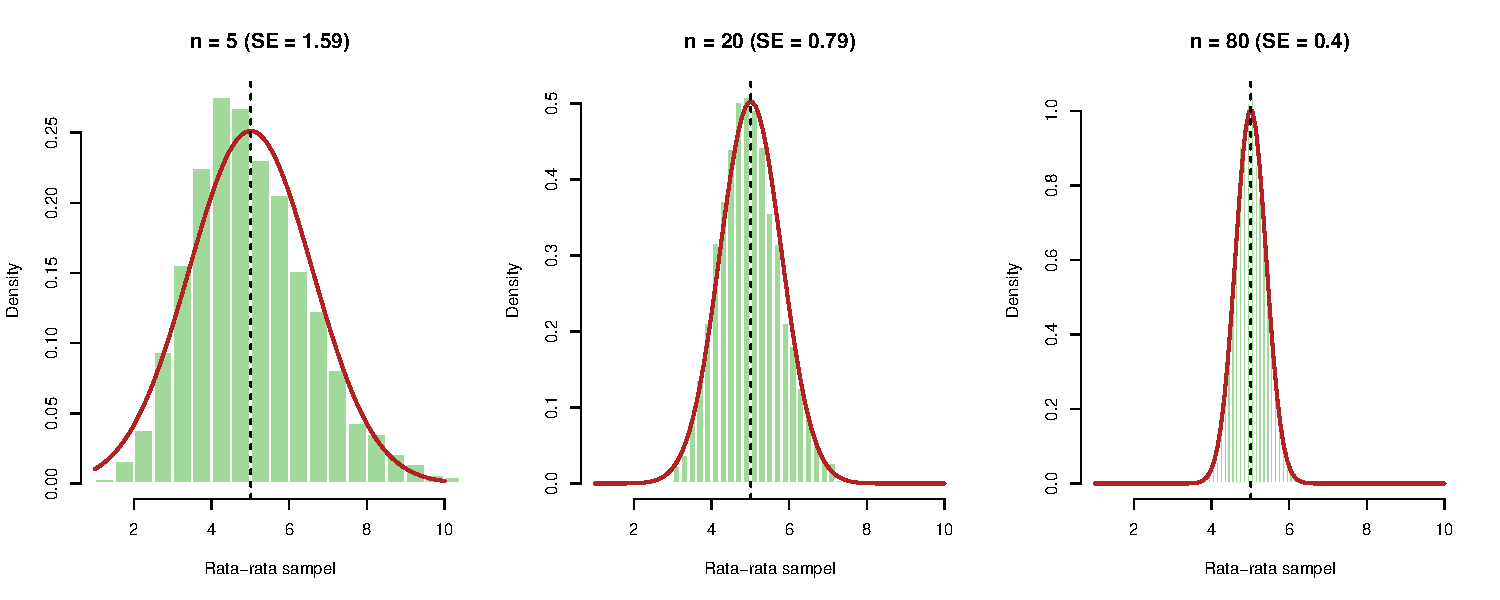
\includegraphics[keepaspectratio]{chapters/P09_files/figure-pdf/unnamed-chunk-5-1.pdf}}

\begin{Shaded}
\begin{Highlighting}[]
\FunctionTok{par}\NormalTok{(}\AttributeTok{mfrow =} \FunctionTok{c}\NormalTok{(}\DecValTok{1}\NormalTok{, }\DecValTok{1}\NormalTok{))}
\end{Highlighting}
\end{Shaded}

Kurva merah adalah distribusi normal dengan mean \(\mu\) dan SD
\(\sigma / \sqrt{n}\). Semakin besar \(n\):

\begin{enumerate}
\def\labelenumi{\arabic{enumi}.}
\tightlist
\item
  Distribusi semakin sempit.
\item
  Bentuknya semakin mendekati normal meskipun populasinya menjulur
  kanan.
\end{enumerate}

\section{Central Limit Theorem (CLT)}\label{central-limit-theorem-clt}

\textbf{Central Limit Theorem:} Jika sampel acak berukuran \(n\) diambil
dari populasi sembarang bentuk dengan mean \(\mu\) dan simpangan baku
\(\sigma\) (terhingga), maka untuk \(n\) yang cukup besar, distribusi
sampling \(\bar{x}\) mendekati normal:

\[\bar{x} \approx N\left(\mu, \frac{\sigma^2}{n}\right)\]

CLT adalah alasan mengapa distribusi normal muncul di mana-mana dalam
statistika inferensial --- bukan karena data selalu normal, tetapi
karena \textbf{rata-rata dari data cenderung normal}.

\subsection{Demonstrasi pada Tiga Bentuk
Populasi}\label{demonstrasi-pada-tiga-bentuk-populasi}

\begin{Shaded}
\begin{Highlighting}[]
\FunctionTok{set.seed}\NormalTok{(}\DecValTok{3}\NormalTok{)}
\NormalTok{pop\_bentuk }\OtherTok{\textless{}{-}} \FunctionTok{list}\NormalTok{(}
  \StringTok{"Seragam"} \OtherTok{=} \FunctionTok{runif}\NormalTok{(}\DecValTok{20000}\NormalTok{, }\DecValTok{0}\NormalTok{, }\DecValTok{10}\NormalTok{),}
  \StringTok{"Menjulur kanan"} \OtherTok{=} \FunctionTok{rexp}\NormalTok{(}\DecValTok{20000}\NormalTok{, }\AttributeTok{rate =} \FloatTok{0.5}\NormalTok{),}
  \StringTok{"Bimodal"} \OtherTok{=} \FunctionTok{c}\NormalTok{(}\FunctionTok{rnorm}\NormalTok{(}\DecValTok{10000}\NormalTok{, }\DecValTok{2}\NormalTok{, }\FloatTok{0.8}\NormalTok{), }\FunctionTok{rnorm}\NormalTok{(}\DecValTok{10000}\NormalTok{, }\DecValTok{8}\NormalTok{, }\FloatTok{0.8}\NormalTok{))}
\NormalTok{)}
\NormalTok{ukuran }\OtherTok{\textless{}{-}} \FunctionTok{c}\NormalTok{(}\DecValTok{2}\NormalTok{, }\DecValTok{5}\NormalTok{, }\DecValTok{30}\NormalTok{)}

\FunctionTok{par}\NormalTok{(}\AttributeTok{mfrow =} \FunctionTok{c}\NormalTok{(}\DecValTok{4}\NormalTok{, }\DecValTok{3}\NormalTok{), }\AttributeTok{mar =} \FunctionTok{c}\NormalTok{(}\DecValTok{3}\NormalTok{, }\DecValTok{3}\NormalTok{, }\FloatTok{2.5}\NormalTok{, }\DecValTok{1}\NormalTok{))}
\ControlFlowTok{for}\NormalTok{ (nama }\ControlFlowTok{in} \FunctionTok{names}\NormalTok{(pop\_bentuk)) \{}
  \FunctionTok{hist}\NormalTok{(pop\_bentuk[[nama]], }\AttributeTok{breaks =} \DecValTok{40}\NormalTok{, }\AttributeTok{col =} \StringTok{"\#9ecae1"}\NormalTok{, }\AttributeTok{border =} \StringTok{"white"}\NormalTok{,}
       \AttributeTok{main =} \FunctionTok{paste}\NormalTok{(}\StringTok{"Populasi:"}\NormalTok{, nama), }\AttributeTok{xlab =} \StringTok{""}\NormalTok{, }\AttributeTok{ylab =} \StringTok{""}\NormalTok{)}
\NormalTok{\}}
\ControlFlowTok{for}\NormalTok{ (nn }\ControlFlowTok{in}\NormalTok{ ukuran) \{}
  \ControlFlowTok{for}\NormalTok{ (nama }\ControlFlowTok{in} \FunctionTok{names}\NormalTok{(pop\_bentuk)) \{}
\NormalTok{    rata }\OtherTok{\textless{}{-}} \FunctionTok{replicate}\NormalTok{(}\DecValTok{3000}\NormalTok{, }\FunctionTok{mean}\NormalTok{(}\FunctionTok{sample}\NormalTok{(pop\_bentuk[[nama]], nn)))}
    \FunctionTok{hist}\NormalTok{(rata, }\AttributeTok{breaks =} \DecValTok{35}\NormalTok{, }\AttributeTok{col =} \StringTok{"\#a1d99b"}\NormalTok{, }\AttributeTok{border =} \StringTok{"white"}\NormalTok{,}
         \AttributeTok{main =} \FunctionTok{paste0}\NormalTok{(nama, }\StringTok{", n = "}\NormalTok{, nn), }\AttributeTok{xlab =} \StringTok{""}\NormalTok{, }\AttributeTok{ylab =} \StringTok{""}\NormalTok{)}
\NormalTok{  \}}
\NormalTok{\}}
\end{Highlighting}
\end{Shaded}

\pandocbounded{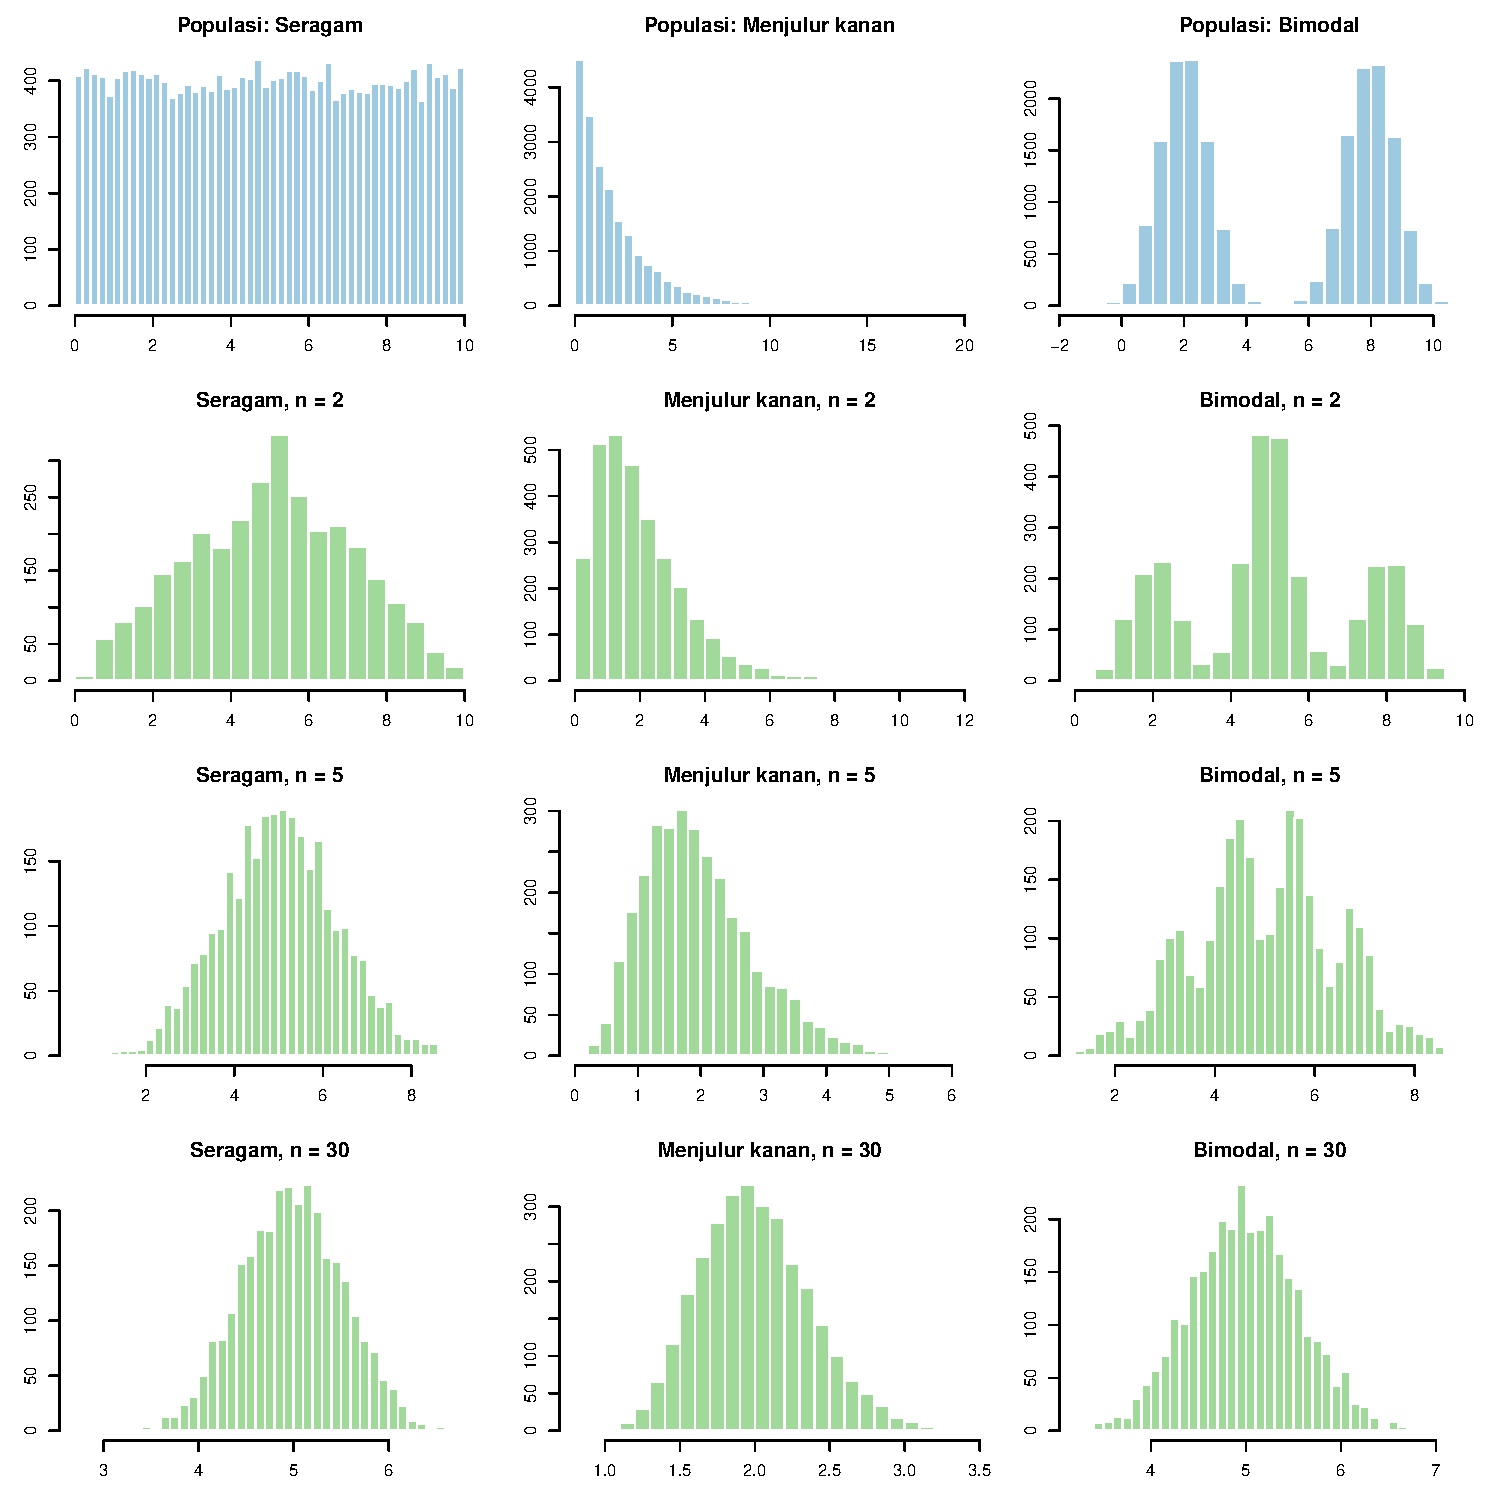
\includegraphics[keepaspectratio]{chapters/P09_files/figure-pdf/unnamed-chunk-7-1.pdf}}

\begin{Shaded}
\begin{Highlighting}[]
\FunctionTok{par}\NormalTok{(}\AttributeTok{mfrow =} \FunctionTok{c}\NormalTok{(}\DecValTok{1}\NormalTok{, }\DecValTok{1}\NormalTok{), }\AttributeTok{mar =} \FunctionTok{c}\NormalTok{(}\DecValTok{5}\NormalTok{, }\DecValTok{4}\NormalTok{, }\DecValTok{4}\NormalTok{, }\DecValTok{2}\NormalTok{) }\SpecialCharTok{+} \FloatTok{0.1}\NormalTok{)}
\end{Highlighting}
\end{Shaded}

Baris pertama adalah populasi; baris berikutnya adalah distribusi
sampling \(\bar{x}\) untuk \(n = 2\), \(5\), dan \(30\). Populasi
seragam sudah tampak lonceng pada \(n = 5\); populasi bimodal masih
bergelombang pada \(n = 2\) tetapi lonceng pada \(n = 30\); populasi
menjulur kanan membutuhkan \(n\) terbesar untuk menghilangkan
kemencengannya.

\subsection{Seberapa Besar ``Cukup
Besar''?}\label{seberapa-besar-cukup-besar}

{\def\LTcaptype{none} % do not increment counter
\begin{longtable}[]{@{}ll@{}}
\toprule\noalign{}
Bentuk populasi & Ukuran sampel yang biasanya cukup \\
\midrule\noalign{}
\endhead
\bottomrule\noalign{}
\endlastfoot
Normal & Berapa pun (distribusi \(\bar{x}\) tepat normal) \\
Simetris, tidak normal & Sekitar 10--15 \\
Menceng sedang & Sekitar 30 (aturan praktis yang populer) \\
Sangat menceng atau banyak outlier & Bisa jauh lebih dari 30 \\
\end{longtable}
}

\begin{Shaded}
\begin{Highlighting}[]
\NormalTok{skew }\OtherTok{\textless{}{-}} \ControlFlowTok{function}\NormalTok{(x) \{ d }\OtherTok{\textless{}{-}}\NormalTok{ x }\SpecialCharTok{{-}} \FunctionTok{mean}\NormalTok{(x); }\FunctionTok{mean}\NormalTok{(d}\SpecialCharTok{\^{}}\DecValTok{3}\NormalTok{) }\SpecialCharTok{/} \FunctionTok{mean}\NormalTok{(d}\SpecialCharTok{\^{}}\DecValTok{2}\NormalTok{)}\SpecialCharTok{\^{}}\FloatTok{1.5}\NormalTok{ \}}
\FunctionTok{set.seed}\NormalTok{(}\DecValTok{4}\NormalTok{)}
\FunctionTok{data.frame}\NormalTok{(}\AttributeTok{n =} \FunctionTok{c}\NormalTok{(}\DecValTok{2}\NormalTok{, }\DecValTok{5}\NormalTok{, }\DecValTok{10}\NormalTok{, }\DecValTok{30}\NormalTok{, }\DecValTok{100}\NormalTok{),}
\AttributeTok{Kemencengan\_xbar =} \FunctionTok{sapply}\NormalTok{(}\FunctionTok{c}\NormalTok{(}\DecValTok{2}\NormalTok{, }\DecValTok{5}\NormalTok{, }\DecValTok{10}\NormalTok{, }\DecValTok{30}\NormalTok{, }\DecValTok{100}\NormalTok{), }\ControlFlowTok{function}\NormalTok{(nn)}
\FunctionTok{round}\NormalTok{(}\FunctionTok{skew}\NormalTok{(}\FunctionTok{replicate}\NormalTok{(}\DecValTok{5000}\NormalTok{, }\FunctionTok{mean}\NormalTok{(}\FunctionTok{sample}\NormalTok{(populasi, nn)))), }\DecValTok{3}\NormalTok{)))}
\end{Highlighting}
\end{Shaded}

\begin{verbatim}
    n Kemencengan_xbar
1   2            1.007
2   5            0.581
3  10            0.470
4  30            0.220
5 100            0.170
\end{verbatim}

Kemencengan distribusi \(\bar{x}\) menyusut kira-kira sebanding dengan
\(1/\sqrt{n}\).

\subsection{Menghitung Peluang dengan
CLT}\label{menghitung-peluang-dengan-clt}

\textbf{Contoh:} Jika diambil sampel acak 40 mahasiswa, berapa peluang
rata-rata waktu layarnya melebihi \(5{,}5\) jam?

\[z = \frac{\bar{x} - \mu}{\sigma / \sqrt{n}}, \qquad P(\bar{x} > 5{,}5) = P(Z > z)\]

\begin{Shaded}
\begin{Highlighting}[]
\NormalTok{se40 }\OtherTok{\textless{}{-}}\NormalTok{ sigma }\SpecialCharTok{/} \FunctionTok{sqrt}\NormalTok{(}\DecValTok{40}\NormalTok{)}
\NormalTok{z\_55 }\OtherTok{\textless{}{-}}\NormalTok{ (}\FloatTok{5.5} \SpecialCharTok{{-}}\NormalTok{ mu) }\SpecialCharTok{/}\NormalTok{ se40}

\FunctionTok{c}\NormalTok{(}\AttributeTok{SE =} \FunctionTok{round}\NormalTok{(se40, }\DecValTok{4}\NormalTok{),}
  \AttributeTok{z =} \FunctionTok{round}\NormalTok{(z\_55, }\DecValTok{3}\NormalTok{),}
  \AttributeTok{Peluang\_CLT =} \FunctionTok{round}\NormalTok{(}\DecValTok{1} \SpecialCharTok{{-}} \FunctionTok{pnorm}\NormalTok{(z\_55), }\DecValTok{4}\NormalTok{),}
  \AttributeTok{Peluang\_simulasi =} \FunctionTok{round}\NormalTok{(}\FunctionTok{mean}\NormalTok{(banyak\_rata }\SpecialCharTok{\textgreater{}} \FloatTok{5.5}\NormalTok{), }\DecValTok{4}\NormalTok{))}
\end{Highlighting}
\end{Shaded}

\begin{verbatim}
              SE                z      Peluang_CLT Peluang_simulasi 
          0.5615           0.8730           0.1913           0.1803 
\end{verbatim}

Perbandingan: peluang \textbf{seorang mahasiswa} (bukan rata-rata 40
orang) memiliki waktu layar di atas \(5{,}5\) jam jauh lebih besar:

\begin{Shaded}
\begin{Highlighting}[]
\FunctionTok{mean}\NormalTok{(populasi }\SpecialCharTok{\textgreater{}} \FloatTok{5.5}\NormalTok{)}
\end{Highlighting}
\end{Shaded}

\begin{verbatim}
[1] 0.35175
\end{verbatim}

Individu sangat bervariasi, tetapi rata-rata dari banyak individu jauh
lebih stabil.

\section{Distribusi Sampling Proporsi
Sampel}\label{distribusi-sampling-proporsi-sampel}

Untuk variabel kategorik biner (Ya/Tidak), statistik yang dipakai adalah
proporsi sampel \(\hat{p} = x / n\).

{\def\LTcaptype{none} % do not increment counter
\begin{longtable}[]{@{}ll@{}}
\toprule\noalign{}
Sifat & Rumus \\
\midrule\noalign{}
\endhead
\bottomrule\noalign{}
\endlastfoot
\textbf{Mean} & \(\mu_{\hat{p}} = p\) \\
\textbf{Standard error} &
\(\sigma_{\hat{p}} = \sqrt{\frac{p(1 - p)}{n}}\) \\
\textbf{Bentuk} & Mendekati normal jika \(np \ge 10\) dan
\(n(1 - p) \ge 10\) \\
\end{longtable}
}

\begin{Shaded}
\begin{Highlighting}[]
\NormalTok{p\_benar }\OtherTok{\textless{}{-}} \FloatTok{0.08} \CommentTok{\# misalnya 8\% mahasiswa pernah terlambat membayar UKT}
\FunctionTok{set.seed}\NormalTok{(}\DecValTok{5}\NormalTok{)}

\FunctionTok{par}\NormalTok{(}\AttributeTok{mfrow =} \FunctionTok{c}\NormalTok{(}\DecValTok{1}\NormalTok{, }\DecValTok{3}\NormalTok{))}
\ControlFlowTok{for}\NormalTok{ (nn }\ControlFlowTok{in} \FunctionTok{c}\NormalTok{(}\DecValTok{20}\NormalTok{, }\DecValTok{60}\NormalTok{, }\DecValTok{300}\NormalTok{)) \{}
\NormalTok{  p\_hat }\OtherTok{\textless{}{-}} \FunctionTok{rbinom}\NormalTok{(}\DecValTok{5000}\NormalTok{, }\AttributeTok{size =}\NormalTok{ nn, }\AttributeTok{prob =}\NormalTok{ p\_benar) }\SpecialCharTok{/}\NormalTok{ nn}
  \FunctionTok{hist}\NormalTok{(p\_hat, }\AttributeTok{breaks =} \FunctionTok{seq}\NormalTok{(}\SpecialCharTok{{-}}\FloatTok{0.005}\NormalTok{, }\FloatTok{0.4}\NormalTok{, }\AttributeTok{by =} \FloatTok{0.01}\NormalTok{), }\AttributeTok{col =} \StringTok{"\#fdae6b"}\NormalTok{,}
       \AttributeTok{border =} \StringTok{"white"}\NormalTok{, }\AttributeTok{freq =} \ConstantTok{FALSE}\NormalTok{, }\AttributeTok{xlim =} \FunctionTok{c}\NormalTok{(}\DecValTok{0}\NormalTok{, }\FloatTok{0.3}\NormalTok{),}
       \AttributeTok{main =} \FunctionTok{paste0}\NormalTok{(}\StringTok{"n = "}\NormalTok{, nn, }\StringTok{": np = "}\NormalTok{, nn }\SpecialCharTok{*}\NormalTok{ p\_benar),}
       \AttributeTok{xlab =} \StringTok{"Proporsi sampel"}\NormalTok{)}
  \FunctionTok{curve}\NormalTok{(}\FunctionTok{dnorm}\NormalTok{(x, p\_benar, }\FunctionTok{sqrt}\NormalTok{(p\_benar }\SpecialCharTok{*}\NormalTok{ (}\DecValTok{1} \SpecialCharTok{{-}}\NormalTok{ p\_benar) }\SpecialCharTok{/}\NormalTok{ nn)),}
        \AttributeTok{add =} \ConstantTok{TRUE}\NormalTok{, }\AttributeTok{col =} \StringTok{"firebrick"}\NormalTok{, }\AttributeTok{lwd =} \DecValTok{2}\NormalTok{)}
\NormalTok{\}}
\end{Highlighting}
\end{Shaded}

\pandocbounded{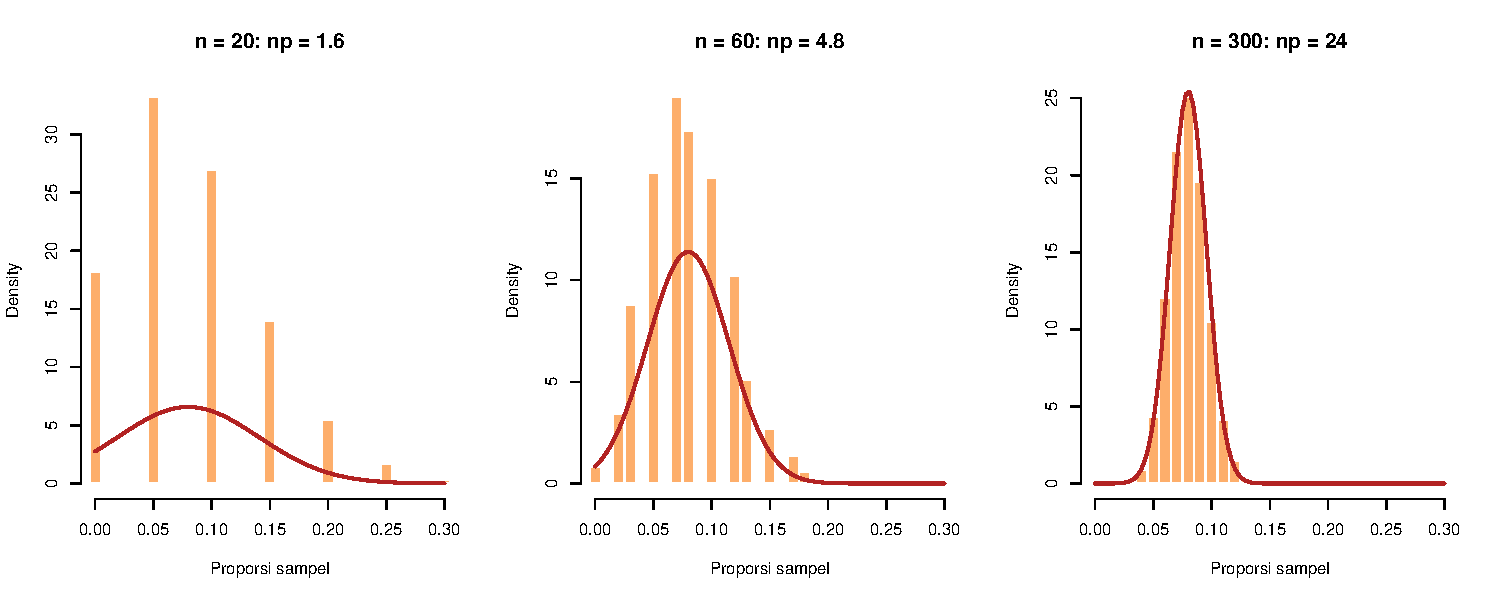
\includegraphics[keepaspectratio]{chapters/P09_files/figure-pdf/unnamed-chunk-12-1.pdf}}

\begin{Shaded}
\begin{Highlighting}[]
\FunctionTok{par}\NormalTok{(}\AttributeTok{mfrow =} \FunctionTok{c}\NormalTok{(}\DecValTok{1}\NormalTok{, }\DecValTok{1}\NormalTok{))}
\end{Highlighting}
\end{Shaded}

Dengan \(n = 20\) (\(np = 1{,}6\)), distribusi \(\hat{p}\) sangat
menceng dan ``berbatang'' --- pendekatan normal buruk. Dengan
\(n = 300\) (\(np = 24\)), pendekatan normal sangat baik.

\section{Standard Error}\label{standard-error}

\subsection{Standard Error vs Simpangan
Baku}\label{standard-error-vs-simpangan-baku}

{\def\LTcaptype{none} % do not increment counter
\begin{longtable}[]{@{}
  >{\raggedright\arraybackslash}p{(\linewidth - 4\tabcolsep) * \real{0.3333}}
  >{\raggedright\arraybackslash}p{(\linewidth - 4\tabcolsep) * \real{0.3333}}
  >{\raggedright\arraybackslash}p{(\linewidth - 4\tabcolsep) * \real{0.3333}}@{}}
\toprule\noalign{}
\begin{minipage}[b]{\linewidth}\raggedright
Aspek
\end{minipage} & \begin{minipage}[b]{\linewidth}\raggedright
Simpangan baku (\(s\) atau \(\sigma\))
\end{minipage} & \begin{minipage}[b]{\linewidth}\raggedright
Standard error (\(SE\))
\end{minipage} \\
\midrule\noalign{}
\endhead
\bottomrule\noalign{}
\endlastfoot
\textbf{Mengukur sebaran} & Data individu & Statistik (misalnya
\(\bar{x}\)) dari sampel ke sampel \\
\textbf{Menjawab} & ``Seberapa beragam individu?'' & ``Seberapa tepat
taksiran kita?'' \\
\textbf{Jika \(n\) bertambah} & Tetap (mendekati \(\sigma\)) &
Mengecil \\
\textbf{Rumus (mean)} &
\(s = \sqrt{\frac{\sum(x_i - \bar{x})^2}{n - 1}}\) &
\(SE = \frac{s}{\sqrt{n}}\) \\
\end{longtable}
}

Karena \(\sigma\) biasanya tidak diketahui, \(SE\) ditaksir dengan
\(s/\sqrt{n}\) (untuk mean) atau \(\sqrt{\hat{p}(1 - \hat{p})/n}\)
(untuk proporsi).

\begin{Shaded}
\begin{Highlighting}[]
\FunctionTok{set.seed}\NormalTok{(}\DecValTok{6}\NormalTok{)}
\NormalTok{n\_besar }\OtherTok{\textless{}{-}} \FunctionTok{c}\NormalTok{(}\DecValTok{10}\NormalTok{, }\DecValTok{40}\NormalTok{, }\DecValTok{160}\NormalTok{, }\DecValTok{640}\NormalTok{)}

\NormalTok{knitr}\SpecialCharTok{::}\FunctionTok{kable}\NormalTok{(}\FunctionTok{t}\NormalTok{(}\FunctionTok{sapply}\NormalTok{(n\_besar, }\ControlFlowTok{function}\NormalTok{(nn) \{}
\NormalTok{  hasil }\OtherTok{\textless{}{-}} \FunctionTok{replicate}\NormalTok{(}\DecValTok{2000}\NormalTok{, \{}
\NormalTok{    s }\OtherTok{\textless{}{-}} \FunctionTok{sample}\NormalTok{(populasi, nn)}
    \FunctionTok{c}\NormalTok{(}\FunctionTok{sd}\NormalTok{(s), }\FunctionTok{sd}\NormalTok{(s) }\SpecialCharTok{/} \FunctionTok{sqrt}\NormalTok{(nn))}
\NormalTok{  \})}
  \FunctionTok{c}\NormalTok{(}\AttributeTok{n =}\NormalTok{ nn,}
    \AttributeTok{Rata\_SD\_sampel =} \FunctionTok{round}\NormalTok{(}\FunctionTok{mean}\NormalTok{(hasil[}\DecValTok{1}\NormalTok{, ]), }\DecValTok{3}\NormalTok{),}
    \AttributeTok{Rata\_SE\_taksiran =} \FunctionTok{round}\NormalTok{(}\FunctionTok{mean}\NormalTok{(hasil[}\DecValTok{2}\NormalTok{, ]), }\DecValTok{3}\NormalTok{))}
\NormalTok{\})), }\AttributeTok{caption =} \FunctionTok{paste0}\NormalTok{(}\StringTok{"Rata{-}rata dari 2.000 sampel per n: SD stabil di sekitar sigma = "}\NormalTok{,}
                      \FunctionTok{round}\NormalTok{(sigma, }\DecValTok{2}\NormalTok{), }\StringTok{", SE mengecil"}\NormalTok{))}
\end{Highlighting}
\end{Shaded}

\begin{longtable}[]{@{}rrr@{}}
\caption{Rata-rata dari 2.000 sampel per n: SD stabil di sekitar sigma =
3.55, SE mengecil}\tabularnewline
\toprule\noalign{}
n & Rata\_SD\_sampel & Rata\_SE\_taksiran \\
\midrule\noalign{}
\endfirsthead
\toprule\noalign{}
n & Rata\_SD\_sampel & Rata\_SE\_taksiran \\
\midrule\noalign{}
\endhead
\bottomrule\noalign{}
\endlastfoot
10 & 3.348 & 1.059 \\
40 & 3.493 & 0.552 \\
160 & 3.537 & 0.280 \\
640 & 3.551 & 0.140 \\
\end{longtable}

\subsection{Hukum Akar Kuadrat}\label{hukum-akar-kuadrat}

Karena \(SE \propto 1/\sqrt{n}\), untuk membagi dua \(SE\) dibutuhkan
sampel \textbf{empat kali lipat}. Presisi semakin mahal: menambah \(n\)
dari 100 ke 400 memberi keuntungan yang sama dengan dari 400 ke 1.600.

\begin{Shaded}
\begin{Highlighting}[]
\NormalTok{n\_seq }\OtherTok{\textless{}{-}} \DecValTok{10}\SpecialCharTok{:}\DecValTok{1000}
\FunctionTok{plot}\NormalTok{(n\_seq, sigma }\SpecialCharTok{/} \FunctionTok{sqrt}\NormalTok{(n\_seq), }\AttributeTok{type =} \StringTok{"l"}\NormalTok{, }\AttributeTok{lwd =} \DecValTok{2}\NormalTok{, }\AttributeTok{col =} \StringTok{"\#4C72B0"}\NormalTok{,}
     \AttributeTok{xlab =} \StringTok{"Ukuran sampel (n)"}\NormalTok{, }\AttributeTok{ylab =} \StringTok{"Standard error"}\NormalTok{,}
     \AttributeTok{main =} \StringTok{"SE Menurun Cepat di Awal, Lalu Melandai"}\NormalTok{)}
\FunctionTok{points}\NormalTok{(}\FunctionTok{c}\NormalTok{(}\DecValTok{100}\NormalTok{, }\DecValTok{400}\NormalTok{), sigma }\SpecialCharTok{/} \FunctionTok{sqrt}\NormalTok{(}\FunctionTok{c}\NormalTok{(}\DecValTok{100}\NormalTok{, }\DecValTok{400}\NormalTok{)), }\AttributeTok{pch =} \DecValTok{16}\NormalTok{, }\AttributeTok{col =} \StringTok{"firebrick"}\NormalTok{, }\AttributeTok{cex =} \FloatTok{1.3}\NormalTok{)}
\FunctionTok{text}\NormalTok{(}\FunctionTok{c}\NormalTok{(}\DecValTok{100}\NormalTok{, }\DecValTok{400}\NormalTok{), sigma }\SpecialCharTok{/} \FunctionTok{sqrt}\NormalTok{(}\FunctionTok{c}\NormalTok{(}\DecValTok{100}\NormalTok{, }\DecValTok{400}\NormalTok{)), }\AttributeTok{pos =} \DecValTok{3}\NormalTok{,}
     \AttributeTok{labels =} \FunctionTok{paste0}\NormalTok{(}\StringTok{"n = "}\NormalTok{, }\FunctionTok{c}\NormalTok{(}\DecValTok{100}\NormalTok{, }\DecValTok{400}\NormalTok{), }\StringTok{"}\SpecialCharTok{\textbackslash{}n}\StringTok{SE = "}\NormalTok{, }\FunctionTok{round}\NormalTok{(sigma }\SpecialCharTok{/} \FunctionTok{sqrt}\NormalTok{(}\FunctionTok{c}\NormalTok{(}\DecValTok{100}\NormalTok{, }\DecValTok{400}\NormalTok{)), }\DecValTok{2}\NormalTok{)))}
\end{Highlighting}
\end{Shaded}

\pandocbounded{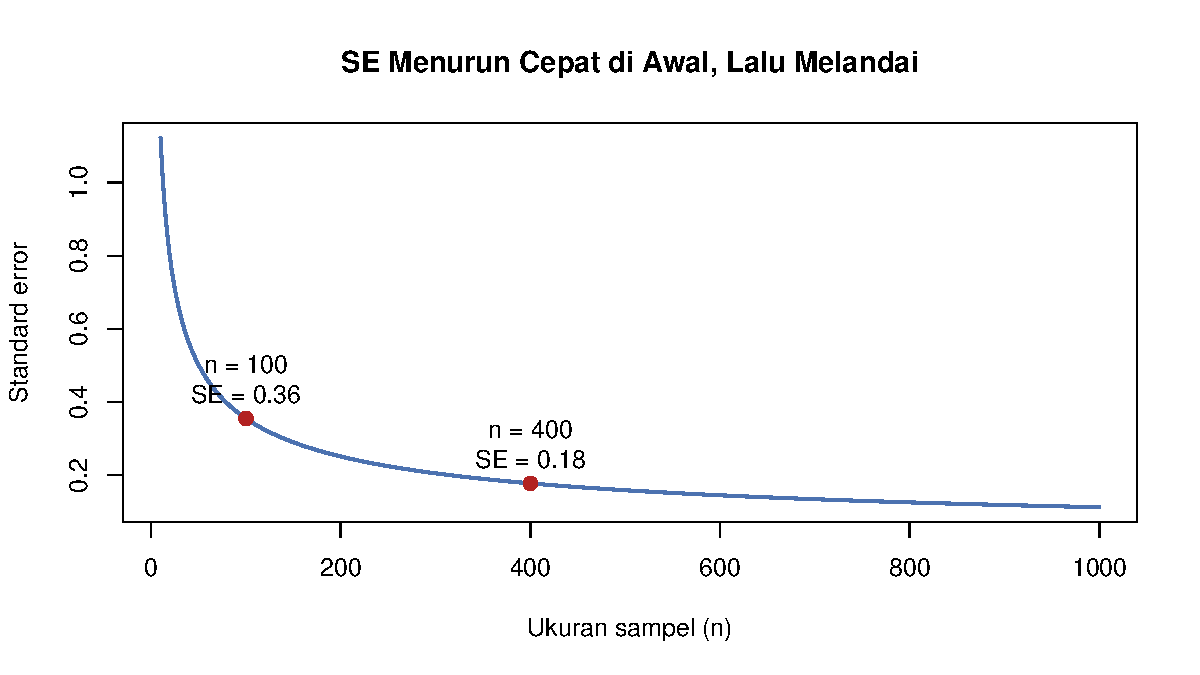
\includegraphics[keepaspectratio]{chapters/P09_files/figure-pdf/unnamed-chunk-15-1.pdf}}

\section{Estimasi}\label{estimasi}

\subsection{Point Estimate}\label{point-estimate}

\emph{Point estimate} adalah satu angka yang menaksir parameter.

{\def\LTcaptype{none} % do not increment counter
\begin{longtable}[]{@{}lll@{}}
\toprule\noalign{}
Parameter & Point estimate & Penaksir tak bias? \\
\midrule\noalign{}
\endhead
\bottomrule\noalign{}
\endlastfoot
\(\mu\) & \(\bar{x}\) & Ya \\
\(p\) & \(\hat{p}\) & Ya \\
\(\sigma^2\) & \(s^2\) (pembagi \(n - 1\)) & Ya \\
\(\sigma\) & \(s\) & Sedikit bias (diabaikan dalam praktik) \\
\end{longtable}
}

Kelemahan \emph{point estimate}: hampir pasti tidak tepat sama dengan
parameter, dan tidak memberi tahu seberapa jauh melesetnya.

\subsection{Confidence Interval (Selang
Kepercayaan)}\label{confidence-interval-selang-kepercayaan}

Selang kepercayaan memberikan rentang nilai yang masuk akal bagi
parameter:

\[\text{Point estimate} \pm \underbrace{\text{nilai kritis} \times SE}_{\text{margin of error}}\]

\subsubsection{\texorpdfstring{CI untuk Mean, \(\sigma\) Diketahui
(\(z\))}{CI untuk Mean, \textbackslash sigma Diketahui (z)}}\label{ci-untuk-mean-sigma-diketahui-z}

\[\bar{x} \pm z_{\alpha/2} \frac{\sigma}{\sqrt{n}}\]

{\def\LTcaptype{none} % do not increment counter
\begin{longtable}[]{@{}lll@{}}
\toprule\noalign{}
Tingkat kepercayaan & \(\alpha\) & \(z_{\alpha/2}\) \\
\midrule\noalign{}
\endhead
\bottomrule\noalign{}
\endlastfoot
90\% & 0,10 & 1,645 \\
95\% & 0,05 & 1,960 \\
99\% & 0,01 & 2,576 \\
\end{longtable}
}

\begin{Shaded}
\begin{Highlighting}[]
\FunctionTok{round}\NormalTok{(}\FunctionTok{qnorm}\NormalTok{(}\FunctionTok{c}\NormalTok{(}\FloatTok{0.95}\NormalTok{, }\FloatTok{0.975}\NormalTok{, }\FloatTok{0.995}\NormalTok{)), }\DecValTok{3}\NormalTok{)}
\end{Highlighting}
\end{Shaded}

\begin{verbatim}
[1] 1.645 1.960 2.576
\end{verbatim}

\subsubsection{\texorpdfstring{CI untuk Mean, \(\sigma\) Tidak Diketahui
(\(t\))}{CI untuk Mean, \textbackslash sigma Tidak Diketahui (t)}}\label{ci-untuk-mean-sigma-tidak-diketahui-t}

Dalam praktik \(\sigma\) hampir tidak pernah diketahui dan diganti
\(s\). Penggantian ini menambah ketidakpastian, sehingga nilai kritis
diambil dari distribusi \(t\) dengan derajat bebas \(df = n - 1\):

\[\bar{x} \pm t_{\alpha/2,\, n-1} \frac{s}{\sqrt{n}}\]

\begin{Shaded}
\begin{Highlighting}[]
\FunctionTok{curve}\NormalTok{(}\FunctionTok{dnorm}\NormalTok{(x), }\SpecialCharTok{{-}}\DecValTok{4}\NormalTok{, }\DecValTok{4}\NormalTok{, }\AttributeTok{lwd =} \DecValTok{2}\NormalTok{, }\AttributeTok{ylab =} \StringTok{"Kepadatan"}\NormalTok{, }\AttributeTok{xlab =} \StringTok{"Nilai"}\NormalTok{,}
\AttributeTok{main =} \StringTok{"Distribusi t Berekor Lebih Tebal dari Normal"}\NormalTok{)}
\FunctionTok{curve}\NormalTok{(}\FunctionTok{dt}\NormalTok{(x, }\AttributeTok{df =} \DecValTok{3}\NormalTok{), }\AttributeTok{add =} \ConstantTok{TRUE}\NormalTok{, }\AttributeTok{lwd =} \DecValTok{2}\NormalTok{, }\AttributeTok{lty =} \DecValTok{2}\NormalTok{, }\AttributeTok{col =} \StringTok{"firebrick"}\NormalTok{)}
\FunctionTok{curve}\NormalTok{(}\FunctionTok{dt}\NormalTok{(x, }\AttributeTok{df =} \DecValTok{10}\NormalTok{), }\AttributeTok{add =} \ConstantTok{TRUE}\NormalTok{, }\AttributeTok{lwd =} \DecValTok{2}\NormalTok{, }\AttributeTok{lty =} \DecValTok{3}\NormalTok{, }\AttributeTok{col =} \StringTok{"darkorange"}\NormalTok{)}
\FunctionTok{legend}\NormalTok{(}\StringTok{"topright"}\NormalTok{, }\AttributeTok{bty =} \StringTok{"n"}\NormalTok{, }\AttributeTok{lwd =} \DecValTok{2}\NormalTok{, }\AttributeTok{lty =} \FunctionTok{c}\NormalTok{(}\DecValTok{1}\NormalTok{, }\DecValTok{2}\NormalTok{, }\DecValTok{3}\NormalTok{), }\AttributeTok{col =} \FunctionTok{c}\NormalTok{(}\StringTok{"black"}\NormalTok{, }\StringTok{"firebrick"}\NormalTok{, }\StringTok{"darkorange"}\NormalTok{),}
\AttributeTok{legend =} \FunctionTok{c}\NormalTok{(}\StringTok{"Normal baku (z)"}\NormalTok{, }\StringTok{"t, df = 3"}\NormalTok{, }\StringTok{"t, df = 10"}\NormalTok{))}
\end{Highlighting}
\end{Shaded}

\pandocbounded{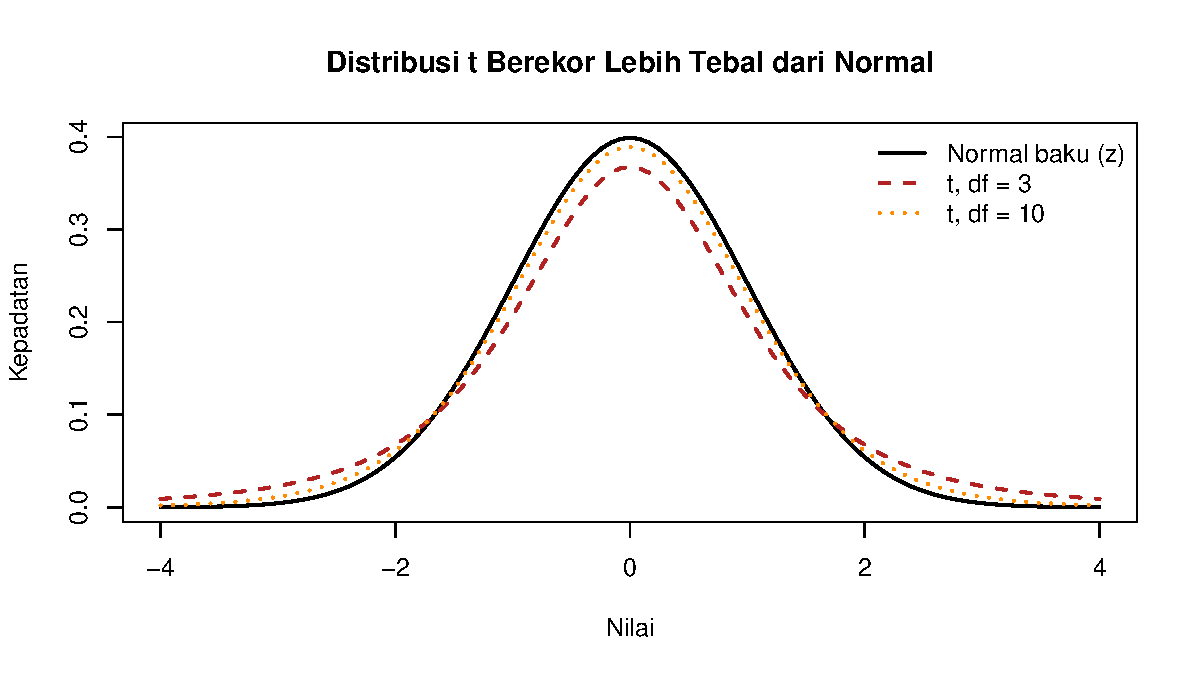
\includegraphics[keepaspectratio]{chapters/P09_files/figure-pdf/unnamed-chunk-17-1.pdf}}

\begin{Shaded}
\begin{Highlighting}[]
\FunctionTok{data.frame}\NormalTok{(}\AttributeTok{df =} \FunctionTok{c}\NormalTok{(}\DecValTok{4}\NormalTok{, }\DecValTok{9}\NormalTok{, }\DecValTok{29}\NormalTok{, }\DecValTok{99}\NormalTok{, }\ConstantTok{Inf}\NormalTok{),}
\AttributeTok{t\_kritis\_95 =} \FunctionTok{round}\NormalTok{(}\FunctionTok{qt}\NormalTok{(}\FloatTok{0.975}\NormalTok{, }\AttributeTok{df =} \FunctionTok{c}\NormalTok{(}\DecValTok{4}\NormalTok{, }\DecValTok{9}\NormalTok{, }\DecValTok{29}\NormalTok{, }\DecValTok{99}\NormalTok{, }\ConstantTok{Inf}\NormalTok{)), }\DecValTok{3}\NormalTok{))}
\end{Highlighting}
\end{Shaded}

\begin{verbatim}
   df t_kritis_95
1   4       2.776
2   9       2.262
3  29       2.045
4  99       1.984
5 Inf       1.960
\end{verbatim}

Untuk sampel kecil, nilai kritis \(t\) lebih besar daripada \(1{,}96\)
(selang lebih lebar, ``hukuman'' karena menaksir \(\sigma\)). Saat \(n\)
membesar, distribusi \(t\) mendekati normal.

\subsubsection{Contoh Perhitungan}\label{contoh-perhitungan}

Satu sampel 40 mahasiswa (\texttt{satu\_sampel}) dipakai untuk menaksir
rata-rata waktu layar seluruh mahasiswa.

\begin{Shaded}
\begin{Highlighting}[]
\NormalTok{n1 }\OtherTok{\textless{}{-}} \FunctionTok{length}\NormalTok{(satu\_sampel)}
\NormalTok{xbar }\OtherTok{\textless{}{-}} \FunctionTok{mean}\NormalTok{(satu\_sampel)}
\NormalTok{s }\OtherTok{\textless{}{-}} \FunctionTok{sd}\NormalTok{(satu\_sampel)}
\NormalTok{t\_krit }\OtherTok{\textless{}{-}} \FunctionTok{qt}\NormalTok{(}\FloatTok{0.975}\NormalTok{, }\AttributeTok{df =}\NormalTok{ n1 }\SpecialCharTok{{-}} \DecValTok{1}\NormalTok{)}
\NormalTok{se\_hat }\OtherTok{\textless{}{-}}\NormalTok{ s }\SpecialCharTok{/} \FunctionTok{sqrt}\NormalTok{(n1)}
\NormalTok{moe }\OtherTok{\textless{}{-}}\NormalTok{ t\_krit }\SpecialCharTok{*}\NormalTok{ se\_hat}

\FunctionTok{c}\NormalTok{(}\AttributeTok{n =}\NormalTok{ n1,}
  \AttributeTok{x\_bar =} \FunctionTok{round}\NormalTok{(xbar, }\DecValTok{3}\NormalTok{),}
  \AttributeTok{s =} \FunctionTok{round}\NormalTok{(s, }\DecValTok{3}\NormalTok{),}
  \AttributeTok{SE =} \FunctionTok{round}\NormalTok{(se\_hat, }\DecValTok{3}\NormalTok{),}
  \AttributeTok{t\_kritis =} \FunctionTok{round}\NormalTok{(t\_krit, }\DecValTok{3}\NormalTok{),}
  \AttributeTok{MoE =} \FunctionTok{round}\NormalTok{(moe, }\DecValTok{3}\NormalTok{),}
  \AttributeTok{Bawah =} \FunctionTok{round}\NormalTok{(xbar }\SpecialCharTok{{-}}\NormalTok{ moe, }\DecValTok{3}\NormalTok{),}
  \AttributeTok{Atas =} \FunctionTok{round}\NormalTok{(xbar }\SpecialCharTok{+}\NormalTok{ moe, }\DecValTok{3}\NormalTok{))}
\end{Highlighting}
\end{Shaded}

\begin{verbatim}
       n    x_bar        s       SE t_kritis      MoE    Bawah     Atas 
  40.000    4.915    3.019    0.477    2.023    0.966    3.950    5.881 
\end{verbatim}

\begin{Shaded}
\begin{Highlighting}[]
\FunctionTok{t.test}\NormalTok{(satu\_sampel, }\AttributeTok{conf.level =} \FloatTok{0.95}\NormalTok{)}\SpecialCharTok{$}\NormalTok{conf.int }\CommentTok{\# fungsi bawaan R, hasil sama}
\end{Highlighting}
\end{Shaded}

\begin{verbatim}
[1] 3.949947 5.881053
attr(,"conf.level")
[1] 0.95
\end{verbatim}

\textbf{Laporan:} \emph{``Rata-rata waktu layar mahasiswa diperkirakan
\(4{,}92\) jam per hari, dengan selang kepercayaan 95\% antara
\(3{,}95\) dan \(5{,}88\) jam (\(n = 40\)).''}

\subsubsection{CI untuk Proporsi}\label{ci-untuk-proporsi}

\[\hat{p} \pm z_{\alpha/2} \sqrt{\frac{\hat{p}(1 - \hat{p})}{n}}, \qquad \text{syarat: } n\hat{p} \ge 10 \text{ dan } n(1 - \hat{p}) \ge 10\]

\begin{Shaded}
\begin{Highlighting}[]
\CommentTok{\# 138 dari 400 responden memakai QRIS setiap hari}
\NormalTok{x\_ya }\OtherTok{\textless{}{-}} \DecValTok{138}
\NormalTok{n\_resp }\OtherTok{\textless{}{-}} \DecValTok{400}
\NormalTok{p\_hat }\OtherTok{\textless{}{-}}\NormalTok{ x\_ya }\SpecialCharTok{/}\NormalTok{ n\_resp}
\NormalTok{se\_p }\OtherTok{\textless{}{-}} \FunctionTok{sqrt}\NormalTok{(p\_hat }\SpecialCharTok{*}\NormalTok{ (}\DecValTok{1} \SpecialCharTok{{-}}\NormalTok{ p\_hat) }\SpecialCharTok{/}\NormalTok{ n\_resp)}
\NormalTok{moe\_p }\OtherTok{\textless{}{-}} \FunctionTok{qnorm}\NormalTok{(}\FloatTok{0.975}\NormalTok{) }\SpecialCharTok{*}\NormalTok{ se\_p}

\FunctionTok{c}\NormalTok{(}\AttributeTok{p\_hat =}\NormalTok{ p\_hat,}
  \AttributeTok{SE =} \FunctionTok{round}\NormalTok{(se\_p, }\DecValTok{4}\NormalTok{),}
  \AttributeTok{MoE =} \FunctionTok{round}\NormalTok{(moe\_p, }\DecValTok{4}\NormalTok{),}
  \AttributeTok{Bawah =} \FunctionTok{round}\NormalTok{(p\_hat }\SpecialCharTok{{-}}\NormalTok{ moe\_p, }\DecValTok{4}\NormalTok{),}
  \AttributeTok{Atas =} \FunctionTok{round}\NormalTok{(p\_hat }\SpecialCharTok{+}\NormalTok{ moe\_p, }\DecValTok{4}\NormalTok{))}
\end{Highlighting}
\end{Shaded}

\begin{verbatim}
 p_hat     SE    MoE  Bawah   Atas 
0.3450 0.0238 0.0466 0.2984 0.3916 
\end{verbatim}

\begin{Shaded}
\begin{Highlighting}[]
\FunctionTok{c}\NormalTok{(}\AttributeTok{n\_p =}\NormalTok{ n\_resp }\SpecialCharTok{*}\NormalTok{ p\_hat, }\AttributeTok{n\_1\_min\_p =}\NormalTok{ n\_resp }\SpecialCharTok{*}\NormalTok{ (}\DecValTok{1} \SpecialCharTok{{-}}\NormalTok{ p\_hat)) }\CommentTok{\# syarat terpenuhi}
\end{Highlighting}
\end{Shaded}

\begin{verbatim}
      n_p n_1_min_p 
      138       262 
\end{verbatim}

\textbf{Laporan:} \emph{``Sekitar \(34{,}5\%\) responden memakai QRIS
setiap hari, margin of error \(\pm 4{,}7\) poin persentase (kepercayaan
95\%).''}

\subsection{Menafsirkan Selang Kepercayaan dengan
Benar}\label{menafsirkan-selang-kepercayaan-dengan-benar}

Kepercayaan 95\% adalah \textbf{sifat prosedurnya}, bukan satu selang
tertentu: jika pengambilan sampel dan perhitungan selang diulang
berkali-kali, sekitar 95\% selang yang dihasilkan akan memuat \(\mu\).

\begin{Shaded}
\begin{Highlighting}[]
\FunctionTok{set.seed}\NormalTok{(}\DecValTok{7}\NormalTok{)}
\NormalTok{B }\OtherTok{\textless{}{-}} \DecValTok{100}
\NormalTok{selang }\OtherTok{\textless{}{-}} \FunctionTok{t}\NormalTok{(}\FunctionTok{replicate}\NormalTok{(B, \{}
\NormalTok{  s\_i }\OtherTok{\textless{}{-}} \FunctionTok{sample}\NormalTok{(populasi, }\DecValTok{40}\NormalTok{)}
\NormalTok{  m }\OtherTok{\textless{}{-}} \FunctionTok{mean}\NormalTok{(s\_i)}
\NormalTok{  e }\OtherTok{\textless{}{-}} \FunctionTok{qt}\NormalTok{(}\FloatTok{0.975}\NormalTok{, }\DecValTok{39}\NormalTok{) }\SpecialCharTok{*} \FunctionTok{sd}\NormalTok{(s\_i) }\SpecialCharTok{/} \FunctionTok{sqrt}\NormalTok{(}\DecValTok{40}\NormalTok{)}
  \FunctionTok{c}\NormalTok{(}\AttributeTok{bawah =}\NormalTok{ m }\SpecialCharTok{{-}}\NormalTok{ e, }\AttributeTok{atas =}\NormalTok{ m }\SpecialCharTok{+}\NormalTok{ e)}
\NormalTok{\}))}
\NormalTok{memuat }\OtherTok{\textless{}{-}}\NormalTok{ selang[, }\StringTok{"bawah"}\NormalTok{] }\SpecialCharTok{\textless{}=}\NormalTok{ mu }\SpecialCharTok{\&}\NormalTok{ selang[, }\StringTok{"atas"}\NormalTok{] }\SpecialCharTok{\textgreater{}=}\NormalTok{ mu}

\FunctionTok{plot}\NormalTok{(}\ConstantTok{NULL}\NormalTok{, }\AttributeTok{xlim =} \FunctionTok{range}\NormalTok{(selang), }\AttributeTok{ylim =} \FunctionTok{c}\NormalTok{(}\DecValTok{1}\NormalTok{, B),}
     \AttributeTok{xlab =} \StringTok{"Waktu layar (jam)"}\NormalTok{, }\AttributeTok{ylab =} \StringTok{"Sampel ke{-}"}\NormalTok{,}
     \AttributeTok{main =} \FunctionTok{paste0}\NormalTok{(}\StringTok{"100 Selang Kepercayaan 95\%: "}\NormalTok{, }\FunctionTok{sum}\NormalTok{(memuat), }\StringTok{" memuat mu"}\NormalTok{))}
\FunctionTok{segments}\NormalTok{(selang[, }\StringTok{"bawah"}\NormalTok{], }\DecValTok{1}\SpecialCharTok{:}\NormalTok{B, selang[, }\StringTok{"atas"}\NormalTok{], }\DecValTok{1}\SpecialCharTok{:}\NormalTok{B,}
         \AttributeTok{col =} \FunctionTok{ifelse}\NormalTok{(memuat, }\StringTok{"grey50"}\NormalTok{, }\StringTok{"firebrick"}\NormalTok{),}
         \AttributeTok{lwd =} \FunctionTok{ifelse}\NormalTok{(memuat, }\DecValTok{1}\NormalTok{, }\FloatTok{2.5}\NormalTok{))}
\FunctionTok{abline}\NormalTok{(}\AttributeTok{v =}\NormalTok{ mu, }\AttributeTok{col =} \StringTok{"\#4C72B0"}\NormalTok{, }\AttributeTok{lwd =} \DecValTok{2}\NormalTok{)}
\end{Highlighting}
\end{Shaded}

\pandocbounded{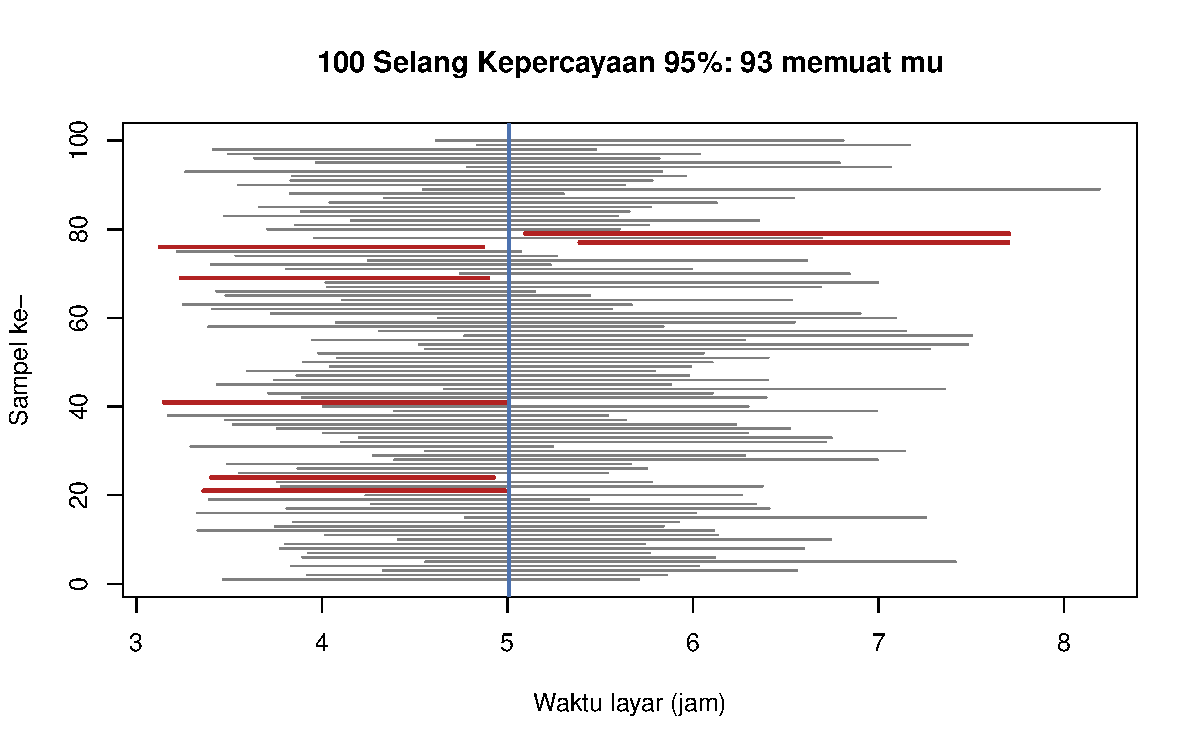
\includegraphics[keepaspectratio]{chapters/P09_files/figure-pdf/unnamed-chunk-23-1.pdf}}

Garis merah adalah selang yang gagal memuat \(\mu\). Kita tidak pernah
tahu apakah selang kita termasuk yang merah, tetapi kita tahu
prosedurnya berhasil sekitar 95\% dari waktu.

{\def\LTcaptype{none} % do not increment counter
\begin{longtable}[]{@{}
  >{\raggedright\arraybackslash}p{(\linewidth - 4\tabcolsep) * \real{0.3333}}
  >{\raggedright\arraybackslash}p{(\linewidth - 4\tabcolsep) * \real{0.3333}}
  >{\raggedright\arraybackslash}p{(\linewidth - 4\tabcolsep) * \real{0.3333}}@{}}
\toprule\noalign{}
\begin{minipage}[b]{\linewidth}\raggedright
Tafsiran
\end{minipage} & \begin{minipage}[b]{\linewidth}\raggedright
Benar/Salah
\end{minipage} & \begin{minipage}[b]{\linewidth}\raggedright
Alasan
\end{minipage} \\
\midrule\noalign{}
\endhead
\bottomrule\noalign{}
\endlastfoot
``Kami 95\% yakin bahwa selang \(4{,}2\)--\(5{,}7\) jam memuat rata-rata
populasi.'' & \textbf{Benar} & Bahasa sehari-hari yang diterima \\
``95\% selang yang dibuat dengan prosedur ini akan memuat \(\mu\).'' &
\textbf{Benar} & Tafsiran paling tepat \\
``Ada peluang 95\% bahwa \(\mu\) berada di antara \(4{,}2\) dan
\(5{,}7\).'' & \textbf{Salah} & \(\mu\) bukan variabel acak; ia di dalam
atau di luar selang \\
``95\% mahasiswa memiliki waktu layar antara \(4{,}2\) dan \(5{,}7\)
jam.'' & \textbf{Salah} & CI adalah tentang rata-rata, bukan individu \\
``95\% rata-rata sampel lain akan jatuh di selang ini.'' &
\textbf{Salah} & CI menaksir parameter \(\mu\), bukan \(\bar{x}\) sampel
berikutnya \\
\end{longtable}
}

\subsection{Faktor yang Memengaruhi Lebar
Selang}\label{faktor-yang-memengaruhi-lebar-selang}

{\def\LTcaptype{none} % do not increment counter
\begin{longtable}[]{@{}
  >{\raggedright\arraybackslash}p{(\linewidth - 4\tabcolsep) * \real{0.3333}}
  >{\raggedright\arraybackslash}p{(\linewidth - 4\tabcolsep) * \real{0.3333}}
  >{\raggedright\arraybackslash}p{(\linewidth - 4\tabcolsep) * \real{0.3333}}@{}}
\toprule\noalign{}
\begin{minipage}[b]{\linewidth}\raggedright
Faktor
\end{minipage} & \begin{minipage}[b]{\linewidth}\raggedright
Jika dinaikkan
\end{minipage} & \begin{minipage}[b]{\linewidth}\raggedright
Dampak pada lebar selang
\end{minipage} \\
\midrule\noalign{}
\endhead
\bottomrule\noalign{}
\endlastfoot
Tingkat kepercayaan (\(90\% \rightarrow 99\%\)) & Nilai kritis naik &
\textbf{Melebar} \\
Ukuran sampel (\(n\)) & \(SE\) turun & \textbf{Menyempit} \\
Variabilitas data (\(s\)) & \(SE\) naik & \textbf{Melebar} \\
\end{longtable}
}

\begin{Shaded}
\begin{Highlighting}[]
\NormalTok{lebar }\OtherTok{\textless{}{-}} \ControlFlowTok{function}\NormalTok{(n, s, conf) \{}
  \DecValTok{2} \SpecialCharTok{*} \FunctionTok{qt}\NormalTok{(}\DecValTok{1} \SpecialCharTok{{-}}\NormalTok{ (}\DecValTok{1} \SpecialCharTok{{-}}\NormalTok{ conf) }\SpecialCharTok{/} \DecValTok{2}\NormalTok{, n }\SpecialCharTok{{-}} \DecValTok{1}\NormalTok{) }\SpecialCharTok{*}\NormalTok{ s }\SpecialCharTok{/} \FunctionTok{sqrt}\NormalTok{(n)}
\NormalTok{\}}

\NormalTok{tabel\_lebar }\OtherTok{\textless{}{-}} \FunctionTok{round}\NormalTok{(}\FunctionTok{outer}\NormalTok{(}\FunctionTok{c}\NormalTok{(}\DecValTok{20}\NormalTok{, }\DecValTok{80}\NormalTok{, }\DecValTok{320}\NormalTok{), }\FunctionTok{c}\NormalTok{(}\FloatTok{0.90}\NormalTok{, }\FloatTok{0.95}\NormalTok{, }\FloatTok{0.99}\NormalTok{),}
                           \FunctionTok{Vectorize}\NormalTok{(}\ControlFlowTok{function}\NormalTok{(n, cf) }\FunctionTok{lebar}\NormalTok{(n, }\AttributeTok{s =} \DecValTok{3}\NormalTok{, }\AttributeTok{conf =}\NormalTok{ cf))), }\DecValTok{3}\NormalTok{)}
\FunctionTok{dimnames}\NormalTok{(tabel\_lebar) }\OtherTok{\textless{}{-}} \FunctionTok{list}\NormalTok{(}\FunctionTok{c}\NormalTok{(}\StringTok{"n = 20"}\NormalTok{, }\StringTok{"n = 80"}\NormalTok{, }\StringTok{"n = 320"}\NormalTok{),}
                              \FunctionTok{c}\NormalTok{(}\StringTok{"90\%"}\NormalTok{, }\StringTok{"95\%"}\NormalTok{, }\StringTok{"99\%"}\NormalTok{))}
\NormalTok{knitr}\SpecialCharTok{::}\FunctionTok{kable}\NormalTok{(tabel\_lebar, }\AttributeTok{caption =} \StringTok{"Lebar CI (s = 3) menurut ukuran sampel dan tingkat kepercayaan"}\NormalTok{)}
\end{Highlighting}
\end{Shaded}

\begin{longtable}[]{@{}lrrr@{}}
\caption{Lebar CI (s = 3) menurut ukuran sampel dan tingkat
kepercayaan}\tabularnewline
\toprule\noalign{}
& 90\% & 95\% & 99\% \\
\midrule\noalign{}
\endfirsthead
\toprule\noalign{}
& 90\% & 95\% & 99\% \\
\midrule\noalign{}
\endhead
\bottomrule\noalign{}
\endlastfoot
n = 20 & 2.320 & 2.808 & 3.838 \\
n = 80 & 1.116 & 1.335 & 1.771 \\
n = 320 & 0.553 & 0.660 & 0.869 \\
\end{longtable}

\section{Menentukan Ukuran Sampel}\label{menentukan-ukuran-sampel}

Sebelum survei, peneliti biasanya menetapkan \emph{margin of error}
(\(E\)) yang diinginkan lalu menghitung \(n\) minimum (\textbf{selalu
dibulatkan ke atas}).

{\def\LTcaptype{none} % do not increment counter
\begin{longtable}[]{@{}
  >{\raggedright\arraybackslash}p{(\linewidth - 4\tabcolsep) * \real{0.3333}}
  >{\raggedright\arraybackslash}p{(\linewidth - 4\tabcolsep) * \real{0.3333}}
  >{\raggedright\arraybackslash}p{(\linewidth - 4\tabcolsep) * \real{0.3333}}@{}}
\toprule\noalign{}
\begin{minipage}[b]{\linewidth}\raggedright
Parameter
\end{minipage} & \begin{minipage}[b]{\linewidth}\raggedright
Rumus ukuran sampel
\end{minipage} & \begin{minipage}[b]{\linewidth}\raggedright
Keterangan
\end{minipage} \\
\midrule\noalign{}
\endhead
\bottomrule\noalign{}
\endlastfoot
\textbf{Mean} & \(n = \left(\frac{z_{\alpha/2}\sigma}{E}\right)^2\) &
\(\sigma\) ditaksir dari studi sebelumnya atau survei percontohan \\
\textbf{Proporsi} & \(n = \frac{z_{\alpha/2}^2 p(1 - p)}{E^2}\) & Jika
\(p\) tidak diketahui, pakai \(p = 0{,}5\) (paling konservatif) \\
\end{longtable}
}

\begin{Shaded}
\begin{Highlighting}[]
\NormalTok{n\_mean }\OtherTok{\textless{}{-}} \ControlFlowTok{function}\NormalTok{(sigma, E, }\AttributeTok{conf =} \FloatTok{0.95}\NormalTok{) }\FunctionTok{ceiling}\NormalTok{((}\FunctionTok{qnorm}\NormalTok{(}\DecValTok{1} \SpecialCharTok{{-}}\NormalTok{ (}\DecValTok{1} \SpecialCharTok{{-}}\NormalTok{ conf) }\SpecialCharTok{/} \DecValTok{2}\NormalTok{) }\SpecialCharTok{*}\NormalTok{ sigma }\SpecialCharTok{/}\NormalTok{ E)}\SpecialCharTok{\^{}}\DecValTok{2}\NormalTok{)}
\NormalTok{n\_prop }\OtherTok{\textless{}{-}} \ControlFlowTok{function}\NormalTok{(E, }\AttributeTok{p =} \FloatTok{0.5}\NormalTok{, }\AttributeTok{conf =} \FloatTok{0.95}\NormalTok{) }\FunctionTok{ceiling}\NormalTok{(}\FunctionTok{qnorm}\NormalTok{(}\DecValTok{1} \SpecialCharTok{{-}}\NormalTok{ (}\DecValTok{1} \SpecialCharTok{{-}}\NormalTok{ conf) }\SpecialCharTok{/} \DecValTok{2}\NormalTok{)}\SpecialCharTok{\^{}}\DecValTok{2} \SpecialCharTok{*}\NormalTok{ p }\SpecialCharTok{*}\NormalTok{ (}\DecValTok{1} \SpecialCharTok{{-}}\NormalTok{ p) }\SpecialCharTok{/}\NormalTok{ E}\SpecialCharTok{\^{}}\DecValTok{2}\NormalTok{)}
\FunctionTok{n\_mean}\NormalTok{(}\AttributeTok{sigma =} \FloatTok{3.5}\NormalTok{, }\AttributeTok{E =} \FloatTok{0.5}\NormalTok{) }\CommentTok{\# menaksir rata{-}rata waktu layar +{-} 0,5 jam}
\end{Highlighting}
\end{Shaded}

\begin{verbatim}
[1] 189
\end{verbatim}

\begin{Shaded}
\begin{Highlighting}[]
\NormalTok{knitr}\SpecialCharTok{::}\FunctionTok{kable}\NormalTok{(}\FunctionTok{data.frame}\NormalTok{(}\AttributeTok{MoE =} \FunctionTok{c}\NormalTok{(}\StringTok{"5\%"}\NormalTok{, }\StringTok{"3\%"}\NormalTok{, }\StringTok{"2\%"}\NormalTok{, }\StringTok{"1\%"}\NormalTok{),}
\AttributeTok{n\_minimum =} \FunctionTok{sapply}\NormalTok{(}\FunctionTok{c}\NormalTok{(}\FloatTok{0.05}\NormalTok{, }\FloatTok{0.03}\NormalTok{, }\FloatTok{0.02}\NormalTok{, }\FloatTok{0.01}\NormalTok{), n\_prop)),}
\AttributeTok{caption =} \StringTok{"Ukuran sampel survei proporsi (p = 0,5; kepercayaan 95\%)"}\NormalTok{)}
\end{Highlighting}
\end{Shaded}

\begin{longtable}[]{@{}lr@{}}
\caption{Ukuran sampel survei proporsi (p = 0,5; kepercayaan
95\%)}\tabularnewline
\toprule\noalign{}
MoE & n\_minimum \\
\midrule\noalign{}
\endfirsthead
\toprule\noalign{}
MoE & n\_minimum \\
\midrule\noalign{}
\endhead
\bottomrule\noalign{}
\endlastfoot
5\% & 385 \\
3\% & 1068 \\
2\% & 2401 \\
1\% & 9604 \\
\end{longtable}

Survei nasional dengan \emph{margin of error} sekitar \(\pm 3\%\)
memerlukan sekitar 1.000--1.100 responden, berapa pun ukuran populasinya
(asalkan populasi jauh lebih besar dari sampel). Memperkecil
\emph{margin of error} dari 2\% ke 1\% memerlukan sampel \textbf{empat
kali lipat}.

\begin{quote}
\textbf{Ukuran sampel tidak menyembuhkan bias.} Rumus di atas hanya
mengendalikan galat acak. Jika metode sampling bias (Pertemuan 3),
sampel sebesar apa pun tetap menghasilkan selang yang presisi di tempat
yang salah.
\end{quote}

\section{Studi Kasus Komprehensif: Survei Adopsi QRIS
UMKM}\label{studi-kasus-komprehensif-survei-adopsi-qris-umkm}

\textbf{Konteks:} Dinas Koperasi ingin menaksir (1) proporsi UMKM
kuliner yang menerima QRIS dan (2) rata-rata nilai transaksi QRIS harian
per UMKM pengguna. Survei acak sederhana terhadap 250 UMKM dari daftar
resmi menghasilkan data berikut.

\begin{Shaded}
\begin{Highlighting}[]
\FunctionTok{set.seed}\NormalTok{(}\DecValTok{2026}\NormalTok{)}
\NormalTok{n\_umkm }\OtherTok{\textless{}{-}} \DecValTok{250}
\NormalTok{terima\_qris }\OtherTok{\textless{}{-}} \FunctionTok{rbinom}\NormalTok{(n\_umkm, }\DecValTok{1}\NormalTok{, }\FloatTok{0.62}\NormalTok{)}
\NormalTok{nilai\_trx }\OtherTok{\textless{}{-}} \FunctionTok{round}\NormalTok{(}\FunctionTok{rlnorm}\NormalTok{(}\FunctionTok{sum}\NormalTok{(terima\_qris), }\AttributeTok{meanlog =} \FunctionTok{log}\NormalTok{(}\DecValTok{450000}\NormalTok{), }\AttributeTok{sdlog =} \FloatTok{0.6}\NormalTok{), }\SpecialCharTok{{-}}\DecValTok{3}\NormalTok{) }\CommentTok{\# Rp/hari}

\FunctionTok{c}\NormalTok{(}\AttributeTok{Jumlah\_pengguna =} \FunctionTok{sum}\NormalTok{(terima\_qris))}
\end{Highlighting}
\end{Shaded}

\begin{verbatim}
Jumlah_pengguna 
            165 
\end{verbatim}

\begin{Shaded}
\begin{Highlighting}[]
\FunctionTok{summary}\NormalTok{(nilai\_trx)}
\end{Highlighting}
\end{Shaded}

\begin{verbatim}
   Min. 1st Qu.  Median    Mean 3rd Qu.    Max. 
  98000  334000  472000  553685  653000 2192000 
\end{verbatim}

\subsection{Langkah 1: Estimasi
Proporsi}\label{langkah-1-estimasi-proporsi}

\begin{Shaded}
\begin{Highlighting}[]
\NormalTok{p\_hat\_u }\OtherTok{\textless{}{-}} \FunctionTok{mean}\NormalTok{(terima\_qris)}
\NormalTok{se\_u }\OtherTok{\textless{}{-}} \FunctionTok{sqrt}\NormalTok{(p\_hat\_u }\SpecialCharTok{*}\NormalTok{ (}\DecValTok{1} \SpecialCharTok{{-}}\NormalTok{ p\_hat\_u) }\SpecialCharTok{/}\NormalTok{ n\_umkm)}
\NormalTok{ci\_u }\OtherTok{\textless{}{-}}\NormalTok{ p\_hat\_u }\SpecialCharTok{+} \FunctionTok{c}\NormalTok{(}\SpecialCharTok{{-}}\DecValTok{1}\NormalTok{, }\DecValTok{1}\NormalTok{) }\SpecialCharTok{*} \FunctionTok{qnorm}\NormalTok{(}\FloatTok{0.975}\NormalTok{) }\SpecialCharTok{*}\NormalTok{ se\_u}

\FunctionTok{c}\NormalTok{(}\AttributeTok{n\_p =}\NormalTok{ n\_umkm }\SpecialCharTok{*}\NormalTok{ p\_hat\_u, }\AttributeTok{n\_1mp =}\NormalTok{ n\_umkm }\SpecialCharTok{*}\NormalTok{ (}\DecValTok{1} \SpecialCharTok{{-}}\NormalTok{ p\_hat\_u)) }\CommentTok{\# cek syarat}
\end{Highlighting}
\end{Shaded}

\begin{verbatim}
  n_p n_1mp 
  165    85 
\end{verbatim}

\begin{Shaded}
\begin{Highlighting}[]
\FunctionTok{round}\NormalTok{(}\FunctionTok{c}\NormalTok{(}\AttributeTok{p\_hat =}\NormalTok{ p\_hat\_u, }\AttributeTok{SE =}\NormalTok{ se\_u, }\AttributeTok{Bawah =}\NormalTok{ ci\_u[}\DecValTok{1}\NormalTok{], }\AttributeTok{Atas =}\NormalTok{ ci\_u[}\DecValTok{2}\NormalTok{]), }\DecValTok{4}\NormalTok{)}
\end{Highlighting}
\end{Shaded}

\begin{verbatim}
 p_hat     SE  Bawah   Atas 
0.6600 0.0300 0.6013 0.7187 
\end{verbatim}

\subsection{Langkah 2: Estimasi Rata-rata Nilai
Transaksi}\label{langkah-2-estimasi-rata-rata-nilai-transaksi}

\begin{Shaded}
\begin{Highlighting}[]
\FunctionTok{hist}\NormalTok{(nilai\_trx }\SpecialCharTok{/} \DecValTok{1000}\NormalTok{, }\AttributeTok{breaks =} \DecValTok{25}\NormalTok{, }\AttributeTok{col =} \StringTok{"\#4C72B0"}\NormalTok{, }\AttributeTok{border =} \StringTok{"white"}\NormalTok{,}
     \AttributeTok{main =} \StringTok{"Nilai Transaksi QRIS Harian (UMKM pengguna)"}\NormalTok{,}
     \AttributeTok{xlab =} \StringTok{"Ribu Rp per hari"}\NormalTok{, }\AttributeTok{ylab =} \StringTok{"Jumlah UMKM"}\NormalTok{)}
\end{Highlighting}
\end{Shaded}

\pandocbounded{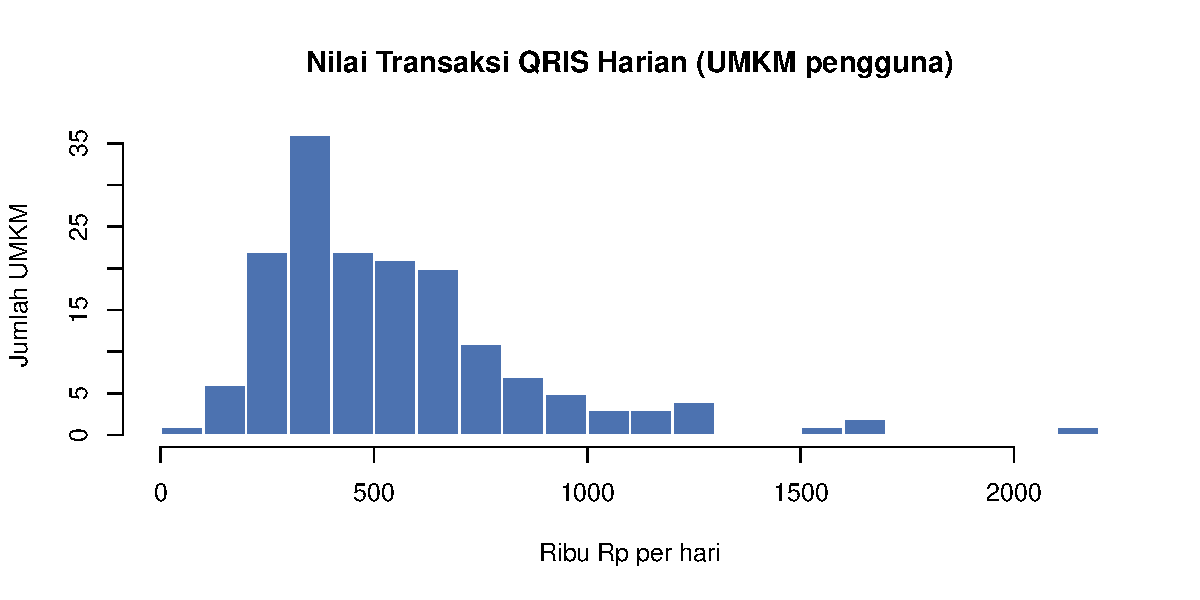
\includegraphics[keepaspectratio]{chapters/P09_files/figure-pdf/unnamed-chunk-30-1.pdf}}

\begin{Shaded}
\begin{Highlighting}[]
\NormalTok{ci\_trx }\OtherTok{\textless{}{-}} \FunctionTok{t.test}\NormalTok{(nilai\_trx)}\SpecialCharTok{$}\NormalTok{conf.int}
\FunctionTok{round}\NormalTok{(}\FunctionTok{c}\NormalTok{(}\AttributeTok{n =} \FunctionTok{length}\NormalTok{(nilai\_trx),}
        \AttributeTok{Mean =} \FunctionTok{mean}\NormalTok{(nilai\_trx),}
        \AttributeTok{Median =} \FunctionTok{median}\NormalTok{(nilai\_trx),}
        \AttributeTok{SE =} \FunctionTok{sd}\NormalTok{(nilai\_trx) }\SpecialCharTok{/} \FunctionTok{sqrt}\NormalTok{(}\FunctionTok{length}\NormalTok{(nilai\_trx)),}
        \AttributeTok{Bawah =}\NormalTok{ ci\_trx[}\DecValTok{1}\NormalTok{],}
        \AttributeTok{Atas =}\NormalTok{ ci\_trx[}\DecValTok{2}\NormalTok{]))}
\end{Highlighting}
\end{Shaded}

\begin{verbatim}
     n   Mean Median     SE  Bawah   Atas 
   165 553685 472000  24623 505065 602304 
\end{verbatim}

\subsection{Langkah 3: Apakah CLT Dapat Diandalkan di
Sini?}\label{langkah-3-apakah-clt-dapat-diandalkan-di-sini}

Datanya menjulur kanan. Kita periksa dengan \textbf{bootstrap}:
mengambil ulang sampel (dengan pengembalian) dari data kita sendiri
untuk meniru distribusi sampling \(\bar{x}\).

\begin{Shaded}
\begin{Highlighting}[]
\FunctionTok{set.seed}\NormalTok{(}\DecValTok{11}\NormalTok{)}
\NormalTok{boot\_mean }\OtherTok{\textless{}{-}} \FunctionTok{replicate}\NormalTok{(}\DecValTok{5000}\NormalTok{, }\FunctionTok{mean}\NormalTok{(}\FunctionTok{sample}\NormalTok{(nilai\_trx, }\AttributeTok{replace =} \ConstantTok{TRUE}\NormalTok{)))}

\FunctionTok{hist}\NormalTok{(boot\_mean }\SpecialCharTok{/} \DecValTok{1000}\NormalTok{, }\AttributeTok{breaks =} \DecValTok{40}\NormalTok{, }\AttributeTok{col =} \StringTok{"\#a1d99b"}\NormalTok{, }\AttributeTok{border =} \StringTok{"white"}\NormalTok{, }\AttributeTok{freq =} \ConstantTok{FALSE}\NormalTok{,}
     \AttributeTok{main =} \StringTok{"Distribusi Bootstrap Rata{-}rata Nilai Transaksi"}\NormalTok{,}
     \AttributeTok{xlab =} \StringTok{"Ribu Rp per hari"}\NormalTok{)}
\FunctionTok{curve}\NormalTok{(}\FunctionTok{dnorm}\NormalTok{(x, }\FunctionTok{mean}\NormalTok{(nilai\_trx) }\SpecialCharTok{/} \DecValTok{1000}\NormalTok{, }\FunctionTok{sd}\NormalTok{(nilai\_trx) }\SpecialCharTok{/} \FunctionTok{sqrt}\NormalTok{(}\FunctionTok{length}\NormalTok{(nilai\_trx)) }\SpecialCharTok{/} \DecValTok{1000}\NormalTok{),}
      \AttributeTok{add =} \ConstantTok{TRUE}\NormalTok{, }\AttributeTok{col =} \StringTok{"firebrick"}\NormalTok{, }\AttributeTok{lwd =} \DecValTok{2}\NormalTok{)}
\end{Highlighting}
\end{Shaded}

\pandocbounded{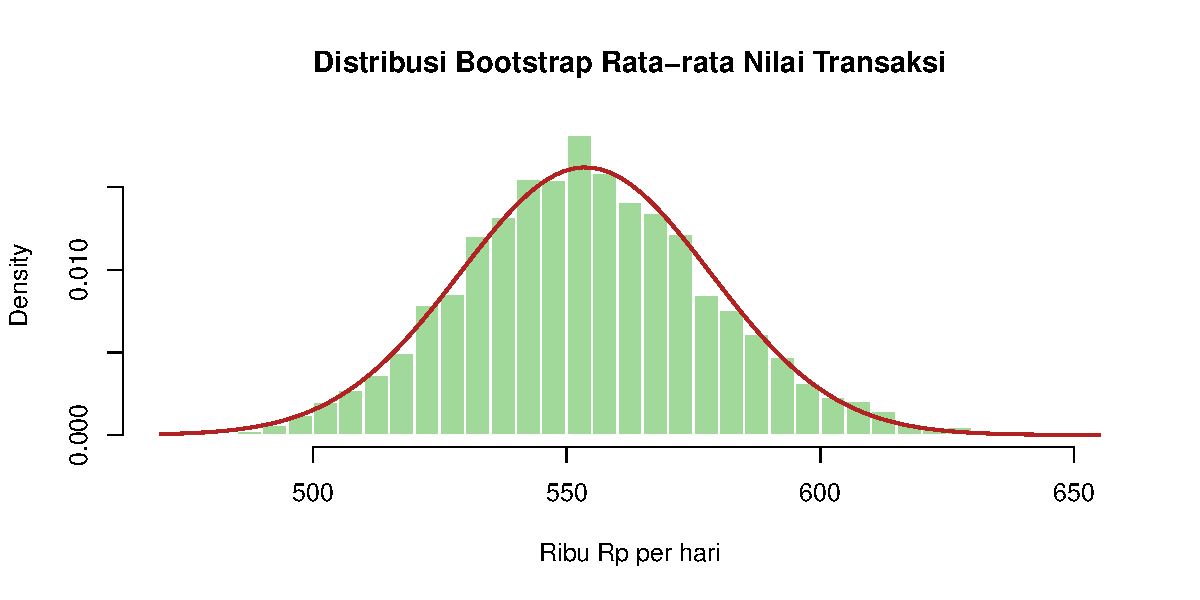
\includegraphics[keepaspectratio]{chapters/P09_files/figure-pdf/unnamed-chunk-32-1.pdf}}

\begin{Shaded}
\begin{Highlighting}[]
\FunctionTok{round}\NormalTok{(}\FunctionTok{quantile}\NormalTok{(boot\_mean, }\FunctionTok{c}\NormalTok{(}\FloatTok{0.025}\NormalTok{, }\FloatTok{0.975}\NormalTok{))) }\CommentTok{\# selang bootstrap persentil 95\%}
\end{Highlighting}
\end{Shaded}

\begin{verbatim}
  2.5%  97.5% 
506082 605874 
\end{verbatim}

Distribusi bootstrap hampir berbentuk lonceng dan selang bootstrap
hampir sama dengan selang \(t\). Dengan \(n = 165\) pengguna, CLT
bekerja baik meskipun data individunya menceng.

\subsection{Langkah 4: Merencanakan Survei
Lanjutan}\label{langkah-4-merencanakan-survei-lanjutan}

Dinas ingin survei tahun depan menghasilkan \emph{margin of error}
proporsi \(\pm 3\%\) dan rata-rata transaksi \(\pm \text{Rp } 30.000\)
(kepercayaan 95\%).

\begin{Shaded}
\begin{Highlighting}[]
\FunctionTok{c}\NormalTok{(}\AttributeTok{n\_untuk\_proporsi =} \FunctionTok{n\_prop}\NormalTok{(}\AttributeTok{E =} \FloatTok{0.03}\NormalTok{, }\AttributeTok{p =}\NormalTok{ p\_hat\_u),}
  \AttributeTok{n\_pengguna\_untuk\_mean =} \FunctionTok{n\_mean}\NormalTok{(}\AttributeTok{sigma =} \FunctionTok{sd}\NormalTok{(nilai\_trx), }\AttributeTok{E =} \DecValTok{30000}\NormalTok{))}
\end{Highlighting}
\end{Shaded}

\begin{verbatim}
     n_untuk_proporsi n_pengguna_untuk_mean 
                  958                   427 
\end{verbatim}

\subsection{Pertanyaan Diskusi dan
Jawaban}\label{pertanyaan-diskusi-dan-jawaban-5}

\begin{enumerate}
\def\labelenumi{\arabic{enumi}.}
\tightlist
\item
  \textbf{Bagaimana melaporkan hasil proporsi?} \emph{``Diperkirakan
  66\% UMKM kuliner telah menerima QRIS (CI 95\%: 60,1\%--71,9\%;
  \(n = 250\)).''} Kalimat ini memuat \emph{point estimate}, selang,
  tingkat kepercayaan, dan ukuran sampel.
\item
  \textbf{Mengapa median transaksi jauh di bawah mean, dan mana yang
  dilaporkan?} Distribusinya menjulur kanan (segelintir UMKM besar).
  Untuk menggambarkan UMKM tipikal, \textbf{median} lebih tepat. Namun
  jika dinas ingin menaksir total nilai transaksi
  (\(\text{mean} \times \text{jumlah UMKM pengguna}\)), yang dibutuhkan
  justru \textbf{mean} beserta selangnya.
\item
  \textbf{Apakah selang 95\% berarti 95\% UMKM bertransaksi di rentang
  tersebut?} \textbf{Tidak.} Selang itu menaksir rata-rata populasi.
  Rentang nilai transaksi individu jauh lebih lebar (lihat histogram).
\item
  \textbf{Mengapa ukuran sampel untuk proporsi tidak dihitung dengan
  \(p = 0{,}5\)?} Kita sudah memiliki taksiran
  \(\hat{p} \approx 0{,}66\) dari survei ini. Memakai \(p = 0{,}5\)
  lebih aman (menghasilkan \(n\) terbesar), tetapi dengan informasi
  sebelumnya kita dapat menghemat biaya. Perbedaannya kecil karena
  \(p(1 - p)\) hampir datar di sekitar \(0{,}5\).
\end{enumerate}

\section{Latihan Mandiri}\label{latihan-mandiri-5}

\subsection{Latihan Utama: Berat Kemasan Kopi
Bubuk}\label{latihan-utama-berat-kemasan-kopi-bubuk}

\textbf{Konteks:} Mesin pengisi kopi bubuk dirancang mengisi kemasan
dengan rata-rata \(250\) gram. Dari data historis, simpangan baku
pengisian \(\sigma = 6\) gram. Petugas QC mengambil sampel acak \(36\)
kemasan.

\begin{Shaded}
\begin{Highlighting}[]
\FunctionTok{set.seed}\NormalTok{(}\DecValTok{99}\NormalTok{)}
\NormalTok{berat }\OtherTok{\textless{}{-}} \FunctionTok{round}\NormalTok{(}\FunctionTok{rnorm}\NormalTok{(}\DecValTok{36}\NormalTok{, }\AttributeTok{mean =} \FloatTok{248.5}\NormalTok{, }\AttributeTok{sd =} \DecValTok{6}\NormalTok{), }\DecValTok{1}\NormalTok{)}
\FunctionTok{summary}\NormalTok{(berat)}
\end{Highlighting}
\end{Shaded}

\begin{verbatim}
   Min. 1st Qu.  Median    Mean 3rd Qu.    Max. 
  230.3   244.9   249.1   247.4   251.4   256.9 
\end{verbatim}

\subsubsection{Tugas 1: Hitung SE dan jelaskan
maknanya}\label{tugas-1-hitung-se-dan-jelaskan-maknanya}

\begin{Shaded}
\begin{Highlighting}[]
\NormalTok{sigma\_k }\OtherTok{\textless{}{-}} \DecValTok{6}
\NormalTok{n\_k }\OtherTok{\textless{}{-}} \FunctionTok{length}\NormalTok{(berat)}
\NormalTok{se\_k }\OtherTok{\textless{}{-}}\NormalTok{ sigma\_k }\SpecialCharTok{/} \FunctionTok{sqrt}\NormalTok{(n\_k)}
\NormalTok{se\_k}
\end{Highlighting}
\end{Shaded}

\begin{verbatim}
[1] 1
\end{verbatim}

\textbf{Jawaban:} \(SE = 6 / \sqrt{36} = 1\) gram. Rata-rata dari 36
kemasan biasanya meleset sekitar 1 gram dari rata-rata sebenarnya ---
jauh lebih kecil daripada variasi berat antarkemasan (6 gram).

\subsubsection{\texorpdfstring{Tugas 2: Jika mesin bekerja benar
(\(\mu = 250\)), berapa peluang rata-rata 36 kemasan kurang dari 248
gram?}{Tugas 2: Jika mesin bekerja benar (\textbackslash mu = 250), berapa peluang rata-rata 36 kemasan kurang dari 248 gram?}}\label{tugas-2-jika-mesin-bekerja-benar-mu-250-berapa-peluang-rata-rata-36-kemasan-kurang-dari-248-gram}

\begin{Shaded}
\begin{Highlighting}[]
\FunctionTok{pnorm}\NormalTok{(}\DecValTok{248}\NormalTok{, }\AttributeTok{mean =} \DecValTok{250}\NormalTok{, }\AttributeTok{sd =}\NormalTok{ sigma\_k }\SpecialCharTok{/} \FunctionTok{sqrt}\NormalTok{(n\_k))}
\end{Highlighting}
\end{Shaded}

\begin{verbatim}
[1] 0.02275013
\end{verbatim}

\textbf{Jawaban:} \(z = (248 - 250) / 1 = -2\) sehingga peluangnya
sekitar \textbf{\(0{,}0228\)} (\(2{,}28\%\)). Kejadian ini jarang jika
mesin bekerja benar --- gagasan yang menjadi dasar uji hipotesis di
Pertemuan 10.

\subsubsection{\texorpdfstring{Tugas 3: Hitung CI 95\% untuk rata-rata
berat (\(\sigma\)
diketahui)}{Tugas 3: Hitung CI 95\% untuk rata-rata berat (\textbackslash sigma diketahui)}}\label{tugas-3-hitung-ci-95-untuk-rata-rata-berat-sigma-diketahui}

\begin{Shaded}
\begin{Highlighting}[]
\NormalTok{ci\_z }\OtherTok{\textless{}{-}} \FunctionTok{mean}\NormalTok{(berat) }\SpecialCharTok{+} \FunctionTok{c}\NormalTok{(}\SpecialCharTok{{-}}\DecValTok{1}\NormalTok{, }\DecValTok{1}\NormalTok{) }\SpecialCharTok{*} \FunctionTok{qnorm}\NormalTok{(}\FloatTok{0.975}\NormalTok{) }\SpecialCharTok{*}\NormalTok{ sigma\_k }\SpecialCharTok{/} \FunctionTok{sqrt}\NormalTok{(n\_k)}
\FunctionTok{round}\NormalTok{(}\FunctionTok{c}\NormalTok{(}\AttributeTok{x\_bar =} \FunctionTok{mean}\NormalTok{(berat), }\AttributeTok{Bawah =}\NormalTok{ ci\_z[}\DecValTok{1}\NormalTok{], }\AttributeTok{Atas =}\NormalTok{ ci\_z[}\DecValTok{2}\NormalTok{]), }\DecValTok{2}\NormalTok{)}
\end{Highlighting}
\end{Shaded}

\begin{verbatim}
 x_bar  Bawah   Atas 
247.40 245.44 249.36 
\end{verbatim}

\subsubsection{\texorpdfstring{Tugas 4: Hitung CI 95\% jika \(\sigma\)
dianggap tidak diketahui
(\(t\))}{Tugas 4: Hitung CI 95\% jika \textbackslash sigma dianggap tidak diketahui (t)}}\label{tugas-4-hitung-ci-95-jika-sigma-dianggap-tidak-diketahui-t}

\begin{Shaded}
\begin{Highlighting}[]
\FunctionTok{round}\NormalTok{(}\FunctionTok{t.test}\NormalTok{(berat)}\SpecialCharTok{$}\NormalTok{conf.int, }\DecValTok{2}\NormalTok{)}
\end{Highlighting}
\end{Shaded}

\begin{verbatim}
[1] 245.25 249.56
attr(,"conf.level")
[1] 0.95
\end{verbatim}

\begin{Shaded}
\begin{Highlighting}[]
\FunctionTok{round}\NormalTok{(}\FunctionTok{c}\NormalTok{(}\AttributeTok{s =} \FunctionTok{sd}\NormalTok{(berat), }\AttributeTok{t\_kritis =} \FunctionTok{qt}\NormalTok{(}\FloatTok{0.975}\NormalTok{, }\DecValTok{35}\NormalTok{), }\AttributeTok{z\_kritis =} \FunctionTok{qnorm}\NormalTok{(}\FloatTok{0.975}\NormalTok{)), }\DecValTok{3}\NormalTok{)}
\end{Highlighting}
\end{Shaded}

\begin{verbatim}
       s t_kritis z_kritis 
   6.366    2.030    1.960 
\end{verbatim}

\subsubsection{Tugas 5: Tafsirkan
hasilnya}\label{tugas-5-tafsirkan-hasilnya}

\textbf{Jawaban:} Selang \(z\) (\([245{,}44;\ 249{,}36]\)) dan selang
\(t\) (\([245{,}25;\ 249{,}56]\)) sangat mirip karena \(n = 36\) cukup
besar (\(t\) kritis hanya sedikit di atas \(1{,}96\)) dan
\(s = 6{,}366\) dekat dengan \(\sigma = 6\). Karena nilai target \(250\)
gram berada di luar selang kepercayaan 95\%, data memberi indikasi bahwa
rata-rata pengisian mesin berbeda dari target --- yang dapat
dikonfirmasi dengan uji hipotesis.

\subsubsection{Tugas 6 (Tantangan): Ukuran
sampel}\label{tugas-6-tantangan-ukuran-sampel}

Berapa kemasan yang harus diambil agar \emph{margin of error} CI 95\%
hanya \(\pm 1\) gram? Dan \(\pm 0{,}5\) gram?

\begin{Shaded}
\begin{Highlighting}[]
\FunctionTok{c}\NormalTok{(}\AttributeTok{MoE\_1 =} \FunctionTok{n\_mean}\NormalTok{(}\AttributeTok{sigma =} \DecValTok{6}\NormalTok{, }\AttributeTok{E =} \DecValTok{1}\NormalTok{),}
  \AttributeTok{MoE\_0.5 =} \FunctionTok{n\_mean}\NormalTok{(}\AttributeTok{sigma =} \DecValTok{6}\NormalTok{, }\AttributeTok{E =} \FloatTok{0.5}\NormalTok{))}
\end{Highlighting}
\end{Shaded}

\begin{verbatim}
  MoE_1 MoE_0.5 
    139     554 
\end{verbatim}

\textbf{Jawaban:} \textbf{139 kemasan} untuk \(\pm 1\) gram dan
\textbf{554 kemasan} untuk \(\pm 0{,}5\) gram --- membagi dua
\emph{margin of error} membutuhkan sampel empat kali lipat.

\subsection{Latihan Tambahan
(Self-Check)}\label{latihan-tambahan-self-check-5}

\subsubsection{Soal A: Waktu Tunggu Layanan
Pelanggan}\label{soal-a-waktu-tunggu-layanan-pelanggan}

Waktu tunggu layanan pelanggan berdistribusi menjulur kanan dengan
\(\mu = 8\) menit dan \(\sigma = 6\) menit. Untuk sampel acak \(64\)
panggilan, tentukan mean, \(SE\), dan bentuk distribusi sampling
\(\bar{x}\), lalu hitung \(P(\bar{x} > 9)\).

\begin{Shaded}
\begin{Highlighting}[]
\CommentTok{\# Kunci jawaban:}
\CommentTok{\# Mean = 8; SE = 6 / sqrt(64) = 0.75; bentuk mendekati normal (CLT, n = 64)}
\DecValTok{1} \SpecialCharTok{{-}} \FunctionTok{pnorm}\NormalTok{(}\DecValTok{9}\NormalTok{, }\AttributeTok{mean =} \DecValTok{8}\NormalTok{, }\AttributeTok{sd =} \FloatTok{0.75}\NormalTok{) }\CommentTok{\# z = 1.33 {-}\textgreater{} sekitar 0.0912}
\end{Highlighting}
\end{Shaded}

\begin{verbatim}
[1] 0.09121122
\end{verbatim}

\subsubsection{Soal B: Survei Dukungan
Kebijakan}\label{soal-b-survei-dukungan-kebijakan}

Survei \(1.200\) pemilih menunjukkan \(54\%\) mendukung sebuah
kebijakan. Hitung CI 95\% dan \emph{margin of error}-nya.

\begin{Shaded}
\begin{Highlighting}[]
\CommentTok{\# Kunci jawaban:}
\NormalTok{p }\OtherTok{\textless{}{-}} \FloatTok{0.54}\NormalTok{; n }\OtherTok{\textless{}{-}} \DecValTok{1200}
\NormalTok{moe }\OtherTok{\textless{}{-}} \FunctionTok{qnorm}\NormalTok{(}\FloatTok{0.975}\NormalTok{) }\SpecialCharTok{*} \FunctionTok{sqrt}\NormalTok{(p }\SpecialCharTok{*}\NormalTok{ (}\DecValTok{1} \SpecialCharTok{{-}}\NormalTok{ p) }\SpecialCharTok{/}\NormalTok{ n) }\CommentTok{\# 0.0282 {-}\textgreater{} +{-} 2.8 poin persentase}
\NormalTok{p }\SpecialCharTok{+} \FunctionTok{c}\NormalTok{(}\SpecialCharTok{{-}}\DecValTok{1}\NormalTok{, }\DecValTok{1}\NormalTok{) }\SpecialCharTok{*}\NormalTok{ moe }\CommentTok{\# 0.512 sampai 0.568}
\end{Highlighting}
\end{Shaded}

\begin{verbatim}
[1] 0.511801 0.568199
\end{verbatim}

\subsubsection{Soal C: Pengukuran pH Air
Limbah}\label{soal-c-pengukuran-ph-air-limbah}

Sepuluh pengukuran pH air limbah:
\texttt{6.8,\ 7.1,\ 6.9,\ 7.4,\ 7.0,\ 6.7,\ 7.2,\ 7.3,\ 6.9,\ 7.1}.
Hitung CI 95\% untuk rata-rata pH secara manual dengan distribusi \(t\)
lalu periksa dengan \texttt{t.test()}.

\begin{Shaded}
\begin{Highlighting}[]
\NormalTok{ph }\OtherTok{\textless{}{-}} \FunctionTok{c}\NormalTok{(}\FloatTok{6.8}\NormalTok{, }\FloatTok{7.1}\NormalTok{, }\FloatTok{6.9}\NormalTok{, }\FloatTok{7.4}\NormalTok{, }\FloatTok{7.0}\NormalTok{, }\FloatTok{6.7}\NormalTok{, }\FloatTok{7.2}\NormalTok{, }\FloatTok{7.3}\NormalTok{, }\FloatTok{6.9}\NormalTok{, }\FloatTok{7.1}\NormalTok{)}
\CommentTok{\# Kunci jawaban:}
\CommentTok{\# x{-}bar = 7.04; s = 0.2171; SE = 0.0687; t(0.975, 9) = 2.262; MoE = 0.155}
\FunctionTok{mean}\NormalTok{(ph) }\SpecialCharTok{+} \FunctionTok{c}\NormalTok{(}\SpecialCharTok{{-}}\DecValTok{1}\NormalTok{, }\DecValTok{1}\NormalTok{) }\SpecialCharTok{*} \FunctionTok{qt}\NormalTok{(}\FloatTok{0.975}\NormalTok{, }\DecValTok{9}\NormalTok{) }\SpecialCharTok{*} \FunctionTok{sd}\NormalTok{(ph) }\SpecialCharTok{/} \FunctionTok{sqrt}\NormalTok{(}\DecValTok{10}\NormalTok{) }\CommentTok{\# 6.885 sampai 7.195}
\end{Highlighting}
\end{Shaded}

\begin{verbatim}
[1] 6.881111 7.198889
\end{verbatim}

\begin{Shaded}
\begin{Highlighting}[]
\FunctionTok{t.test}\NormalTok{(ph)}\SpecialCharTok{$}\NormalTok{conf.int}
\end{Highlighting}
\end{Shaded}

\begin{verbatim}
[1] 6.881111 7.198889
attr(,"conf.level")
[1] 0.95
\end{verbatim}

\subsubsection{Soal D: Evaluasi Tafsiran
Media}\label{soal-d-evaluasi-tafsiran-media}

Sebuah media menulis: \emph{``Dengan CI 95\% {[}62\%, 68\%{]}, berarti
95\% warga memiliki tingkat kepuasan antara 62\% dan 68\%.''} Perbaiki
tafsiran ini.

\begin{Shaded}
\begin{Highlighting}[]
\CommentTok{\# Kunci jawaban:}
\CommentTok{\# Tafsiran keliru. Yang benar: "Kami 95\% yakin bahwa proporsi warga yang puas di seluruh}
\CommentTok{\# populasi berada antara 62\% dan 68\%." CI menaksir PARAMETER populasi (proporsi yang puas),}
\CommentTok{\# bukan rentang nilai individu.}
\end{Highlighting}
\end{Shaded}

\section{Kesalahan Umum dalam Sampling Distribution dan
Estimasi}\label{kesalahan-umum-dalam-sampling-distribution-dan-estimasi}

\begin{enumerate}
\def\labelenumi{\arabic{enumi}.}
\tightlist
\item
  \textbf{Menyamakan distribusi sampel dengan distribusi sampling} ---
  yang pertama berisi data individu, yang kedua berisi statistik dari
  banyak sampel.
\item
  \textbf{Mengira CLT membuat data menjadi normal} --- CLT berbicara
  tentang distribusi rata-rata (\(\bar{x}\)), bukan data individu.
\item
  \textbf{Menganggap \(n \ge 30\) selalu cukup} --- data yang sangat
  menceng atau ber-outlier bisa membutuhkan \(n\) lebih besar.
\item
  \textbf{Menyamakan SD dan SE} --- SD mengukur keragaman individu; SE
  mengukur ketepatan taksiran.
\item
  \textbf{Memakai \(z\) padahal \(\sigma\) tidak diketahui dan \(n\)
  kecil} --- gunakan distribusi \(t\).
\item
  \textbf{Menafsirkan CI sebagai peluang parameter berada di dalam
  selang tertentu}, atau sebagai rentang nilai individu.
\item
  \textbf{Membulatkan ukuran sampel ke bawah} --- selalu bulatkan ke
  atas (\texttt{ceiling()}).
\item
  \textbf{Mengira ukuran populasi menentukan ukuran sampel} --- untuk
  populasi besar, yang menentukan adalah \emph{margin of error}, tingkat
  kepercayaan, dan variabilitas.
\item
  \textbf{Mengira sampel besar menghilangkan bias} --- ukuran sampel
  hanya mengecilkan galat acak.
\item
  \textbf{Memakai pendekatan normal untuk proporsi saat \(n\hat{p}\)
  atau \(n(1 - \hat{p})\) kurang dari 10}.
\item
  \textbf{Melaporkan \emph{point estimate} tanpa selang atau \(n\)} ---
  pembaca tidak dapat menilai ketepatannya.
\end{enumerate}

\section{Cheat Sheet: Fungsi R yang
Digunakan}\label{cheat-sheet-fungsi-r-yang-digunakan-5}

{\def\LTcaptype{none} % do not increment counter
\begin{longtable}[]{@{}
  >{\raggedright\arraybackslash}p{(\linewidth - 2\tabcolsep) * \real{0.5000}}
  >{\raggedright\arraybackslash}p{(\linewidth - 2\tabcolsep) * \real{0.5000}}@{}}
\toprule\noalign{}
\begin{minipage}[b]{\linewidth}\raggedright
Fungsi
\end{minipage} & \begin{minipage}[b]{\linewidth}\raggedright
Kegunaan
\end{minipage} \\
\midrule\noalign{}
\endhead
\bottomrule\noalign{}
\endlastfoot
\texttt{sample(x,\ n)} / \texttt{sample(x,\ replace\ =\ TRUE)} & Sampel
acak / sampel bootstrap \\
\texttt{replicate(B,\ ekspresi)} & Simulasi distribusi sampling \\
\texttt{rgamma()}, \texttt{rexp()}, \texttt{runif()}, \texttt{rnorm()},
\texttt{rbinom()}, \texttt{rlnorm()} & Membangkitkan populasi/data
simulasi \\
\texttt{pnorm(q,\ mean,\ sd)} & Peluang kumulatif normal
\(P(X \le q)\) \\
\texttt{qnorm(p)} & Nilai kritis \(z\) (misalnya \texttt{qnorm(0.975)} =
\(1{,}96\)) \\
\texttt{dnorm(x,\ mean,\ sd)} & Kepadatan normal (untuk menggambar
kurva) \\
\texttt{qt(p,\ df)}, \texttt{pt(q,\ df)}, \texttt{dt(x,\ df)} & Nilai
kritis, peluang, dan kepadatan distribusi \(t\) \\
\texttt{t.test(x,\ conf.level\ =\ 0.95)\$conf.int} & Selang kepercayaan
\(t\) untuk mean \\
\texttt{curve(f(x),\ add\ =\ TRUE)} & Menambahkan kurva teoretis pada
histogram \\
\texttt{segments(x0,\ y0,\ x1,\ y1)} & Menggambar selang kepercayaan
sebagai garis \\
\texttt{ceiling(x)} & Membulatkan ke atas (ukuran sampel) \\
\texttt{outer(a,\ b,\ f)} & Tabel nilai untuk kombinasi dua parameter \\
\texttt{quantile(boot,\ c(0.025,\ 0.975))} & Selang bootstrap
persentil \\
\end{longtable}
}

\section{Glosarium Istilah}\label{glosarium-istilah-5}

{\def\LTcaptype{none} % do not increment counter
\begin{longtable}[]{@{}
  >{\raggedright\arraybackslash}p{(\linewidth - 2\tabcolsep) * \real{0.5000}}
  >{\raggedright\arraybackslash}p{(\linewidth - 2\tabcolsep) * \real{0.5000}}@{}}
\toprule\noalign{}
\begin{minipage}[b]{\linewidth}\raggedright
Istilah
\end{minipage} & \begin{minipage}[b]{\linewidth}\raggedright
Definisi Singkat
\end{minipage} \\
\midrule\noalign{}
\endhead
\bottomrule\noalign{}
\endlastfoot
\textbf{Statistika Inferensial} & Menarik kesimpulan tentang populasi
dari sampel \\
\textbf{Distribusi Sampling} & Distribusi sebuah statistik dari semua
kemungkinan sampel berukuran \(n\) \\
\textbf{Penaksir Tak Bias} & Statistik yang rata-rata distribusi
samplingnya sama dengan parameter \\
\textbf{Central Limit Theorem} & Distribusi \(\bar{x}\) mendekati normal
untuk \(n\) besar, apa pun bentuk populasinya \\
\textbf{Standard Error (SE)} & Simpangan baku distribusi sampling sebuah
statistik \\
\textbf{Koreksi Populasi Terhingga} & Faktor \(\sqrt{(N - n)/(N - 1)}\)
bila sampel lebih dari sekitar 5\% populasi \\
\textbf{Point Estimate} & Satu nilai yang menaksir parameter \\
\textbf{Confidence Interval} & Rentang nilai yang masuk akal bagi
parameter dengan tingkat kepercayaan tertentu \\
\textbf{Tingkat Kepercayaan} & Persentase selang (dari pengulangan
prosedur) yang memuat parameter \\
\textbf{Margin of Error} & Nilai kritis \(\times\) SE; setengah lebar
selang \\
\textbf{Nilai Kritis} & Nilai dari distribusi \(z\) atau \(t\) yang
menentukan lebar selang \\
\textbf{Distribusi \(t\)} & Distribusi berekor tebal yang dipakai bila
\(\sigma\) ditaksir dengan \(s\) \\
\textbf{Derajat Bebas (\(df\))} & Parameter distribusi \(t\); \(n - 1\)
untuk satu mean \\
\textbf{Bootstrap} & Pengambilan sampel ulang dengan pengembalian dari
data untuk meniru distribusi sampling \\
\end{longtable}
}

\section{Rangkuman dan Kesimpulan}\label{rangkuman-dan-kesimpulan-5}

\begin{enumerate}
\def\labelenumi{\arabic{enumi}.}
\tightlist
\item
  Distribusi sampling menggambarkan bagaimana sebuah statistik
  bervariasi dari sampel ke sampel; ia adalah fondasi seluruh statistika
  inferensial.
\item
  \(\bar{x}\) dan \(\hat{p}\) adalah penaksir tak bias dengan \(SE\)
  masing-masing \(\sigma / \sqrt{n}\) dan \(\sqrt{p(1 - p) / n}\).
\item
  CLT menjamin distribusi \(\bar{x}\) mendekati normal untuk \(n\) cukup
  besar, apa pun bentuk populasinya; makin menceng populasi, makin besar
  \(n\) yang dibutuhkan.
\item
  \(SE\) bukan \(SD\): \(SE\) mengecil sebanding \(1/\sqrt{n}\) ---
  presisi dua kali lipat membutuhkan sampel empat kali lipat.
\item
  Selang kepercayaan
  \(= \text{point estimate} \pm \text{nilai kritis} \times SE\). Gunakan
  \(z\) bila \(\sigma\) diketahui, \(t\) bila \(\sigma\) ditaksir.
  Kepercayaan 95\% adalah sifat prosedur, bukan peluang untuk satu
  selang.
\item
  Ukuran sampel dapat direncanakan dari \emph{margin of error} yang
  diinginkan tetapi tidak dapat menyembuhkan bias sampling.
\end{enumerate}

\begin{quote}
\textbf{Jembatan ke sesi berikutnya:} Tugas 2 latihan tadi bertanya,
\emph{``jika mesin bekerja benar, seberapa jarang hasil seperti ini?''}
Pertanyaan itulah inti uji hipotesis di Pertemuan 10: \(H_0\), \(H_1\),
tingkat signifikansi, \emph{p-value}, dan kesalahan Tipe I dan II.
\end{quote}

\bookmarksetup{startatroot}

\chapter{Konsep dan Uji Hipotesis}\label{konsep-dan-uji-hipotesis}

\section{Logika Uji Hipotesis}\label{logika-uji-hipotesis}

Dalam sidang pengadilan berlaku asas praduga tak bersalah: terdakwa
dianggap tidak bersalah sampai jaksa menghadirkan bukti yang cukup kuat
untuk meyakinkan hakim sebaliknya. Jika bukti kurang kuat, putusannya
adalah ``tidak terbukti bersalah'' --- bukan ``terbukti tidak
bersalah''. Hakim juga bisa keliru: menghukum orang yang tidak bersalah,
atau membebaskan orang yang bersalah.

Uji hipotesis bekerja dengan logika yang persis sama. Kita memulai
dengan asumsi ``tidak ada efek/perbedaan'' (\(H_0\)), lalu bertanya:
jika asumsi itu benar, seberapa mengejutkan data yang kita peroleh? Jika
sangat mengejutkan, kita menolak asumsi tersebut.

{\def\LTcaptype{none} % do not increment counter
\begin{longtable}[]{@{}
  >{\raggedright\arraybackslash}p{(\linewidth - 2\tabcolsep) * \real{0.5000}}
  >{\raggedright\arraybackslash}p{(\linewidth - 2\tabcolsep) * \real{0.5000}}@{}}
\toprule\noalign{}
\begin{minipage}[b]{\linewidth}\raggedright
Pengadilan
\end{minipage} & \begin{minipage}[b]{\linewidth}\raggedright
Uji Hipotesis
\end{minipage} \\
\midrule\noalign{}
\endhead
\bottomrule\noalign{}
\endlastfoot
Praduga tak bersalah & \(H_0\) diasumsikan benar \\
Tuduhan jaksa & \(H_1\) (klaim yang ingin dibuktikan) \\
Bukti di persidangan & Data sampel dan statistik uji \\
Standar ``tanpa keraguan yang wajar'' & Tingkat signifikansi
\(\alpha\) \\
Putusan bersalah & Tolak \(H_0\) \\
Putusan tidak terbukti bersalah & Gagal menolak \(H_0\) (bukan
``menerima \(H_0\)'') \\
Menghukum orang tak bersalah & Kesalahan Tipe I \\
Membebaskan orang bersalah & Kesalahan Tipe II \\
\end{longtable}
}

\subsection{Ilustrasi: Apakah Mesin Pengisi Masih
Tepat?}\label{ilustrasi-apakah-mesin-pengisi-masih-tepat}

Melanjutkan latihan Pertemuan 9: mesin kopi bubuk seharusnya mengisi
rata-rata \(250\) gram dengan \(\sigma = 6\) gram. Sampel \(36\) kemasan
menghasilkan \(\bar{x} = 247{,}6\) gram. Apakah mesin perlu dikalibrasi,
atau selisih \(2{,}4\) gram itu sekadar kebetulan sampling?

Jika mesin benar (\(\mu = 250\)), maka menurut CLT
\(\bar{x} \sim N(250, 6/\sqrt{36} = 1)\). Kita lihat seberapa ``jauh''
\(247{,}6\) dari distribusi tersebut:

\begin{Shaded}
\begin{Highlighting}[]
\NormalTok{mu0 }\OtherTok{\textless{}{-}} \DecValTok{250}\NormalTok{; sigma }\OtherTok{\textless{}{-}} \DecValTok{6}\NormalTok{; n }\OtherTok{\textless{}{-}} \DecValTok{36}\NormalTok{; xbar }\OtherTok{\textless{}{-}} \FloatTok{247.6}
\NormalTok{se }\OtherTok{\textless{}{-}}\NormalTok{ sigma }\SpecialCharTok{/} \FunctionTok{sqrt}\NormalTok{(n)}

\FunctionTok{set.seed}\NormalTok{(}\DecValTok{10}\NormalTok{)}
\NormalTok{xbar\_jika\_H0 }\OtherTok{\textless{}{-}} \FunctionTok{replicate}\NormalTok{(}\DecValTok{100000}\NormalTok{, }\FunctionTok{mean}\NormalTok{(}\FunctionTok{rnorm}\NormalTok{(n, mu0, sigma)))}

\FunctionTok{hist}\NormalTok{(xbar\_jika\_H0, }\AttributeTok{breaks =} \DecValTok{60}\NormalTok{, }\AttributeTok{col =} \StringTok{"\#c6dbef"}\NormalTok{, }\AttributeTok{border =} \StringTok{"white"}\NormalTok{, }\AttributeTok{freq =} \ConstantTok{FALSE}\NormalTok{,}
     \AttributeTok{main =} \StringTok{"Distribusi x{-}bar JIKA mesin bekerja benar (mu = 250)"}\NormalTok{,}
     \AttributeTok{xlab =} \StringTok{"Rata{-}rata 36 kemasan (gram)"}\NormalTok{)}
\FunctionTok{abline}\NormalTok{(}\AttributeTok{v =} \FunctionTok{c}\NormalTok{(xbar, }\DecValTok{2} \SpecialCharTok{*}\NormalTok{ mu0 }\SpecialCharTok{{-}}\NormalTok{ xbar), }\AttributeTok{col =} \StringTok{"firebrick"}\NormalTok{, }\AttributeTok{lwd =} \DecValTok{2}\NormalTok{, }\AttributeTok{lty =} \FunctionTok{c}\NormalTok{(}\DecValTok{1}\NormalTok{, }\DecValTok{2}\NormalTok{))}
\end{Highlighting}
\end{Shaded}

\pandocbounded{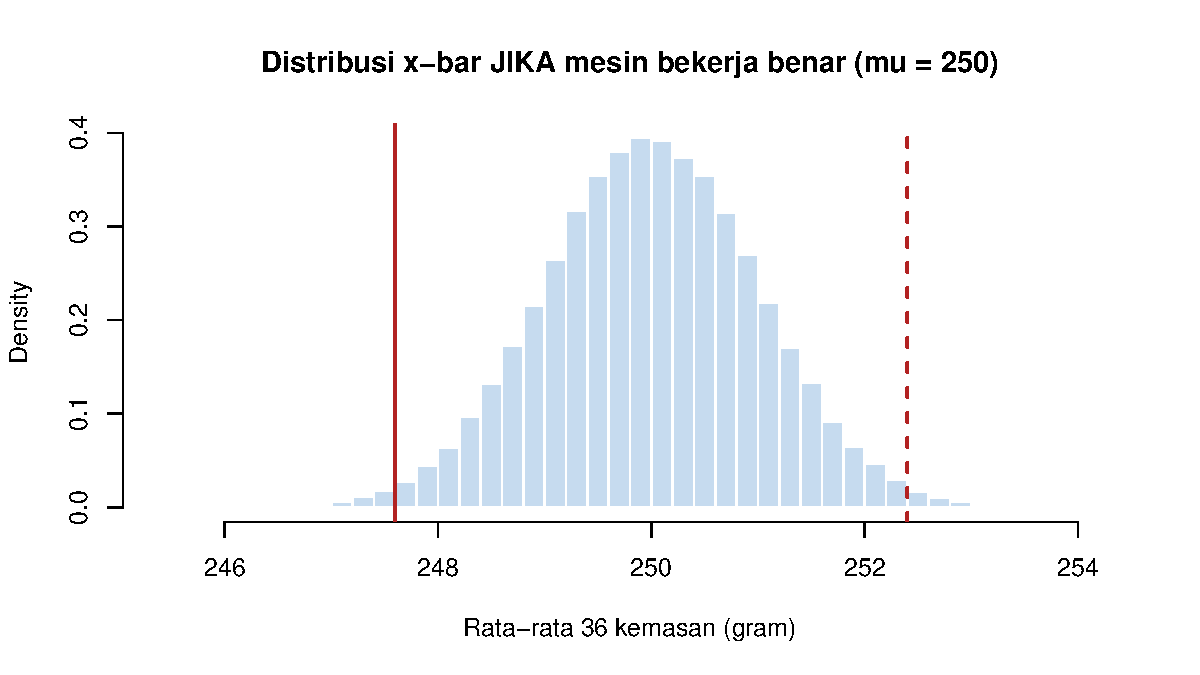
\includegraphics[keepaspectratio]{chapters/P10_files/figure-pdf/unnamed-chunk-1-1.pdf}}

\begin{Shaded}
\begin{Highlighting}[]
\FunctionTok{mean}\NormalTok{(}\FunctionTok{abs}\NormalTok{(xbar\_jika\_H0 }\SpecialCharTok{{-}}\NormalTok{ mu0) }\SpecialCharTok{\textgreater{}=} \FunctionTok{abs}\NormalTok{(xbar }\SpecialCharTok{{-}}\NormalTok{ mu0)) }\CommentTok{\# seberapa sering selisih sebesar ini terjadi}
\end{Highlighting}
\end{Shaded}

\begin{verbatim}
[1] 0.01579
\end{verbatim}

Jika mesin benar, rata-rata yang meleset \(2{,}4\) gram atau lebih (ke
arah mana pun) hanya terjadi sekitar \(1{,}6\%\) dari waktu. Angka
inilah yang disebut \emph{p-value}. Karena sangat jarang, kita punya
alasan kuat untuk meragukan bahwa mesin bekerja benar.

\section{Merumuskan Hipotesis}\label{merumuskan-hipotesis}

\subsection{Hipotesis Nol dan
Alternatif}\label{hipotesis-nol-dan-alternatif}

{\def\LTcaptype{none} % do not increment counter
\begin{longtable}[]{@{}
  >{\raggedright\arraybackslash}p{(\linewidth - 4\tabcolsep) * \real{0.3333}}
  >{\raggedright\arraybackslash}p{(\linewidth - 4\tabcolsep) * \real{0.3333}}
  >{\raggedright\arraybackslash}p{(\linewidth - 4\tabcolsep) * \real{0.3333}}@{}}
\toprule\noalign{}
\begin{minipage}[b]{\linewidth}\raggedright
Aspek
\end{minipage} & \begin{minipage}[b]{\linewidth}\raggedright
Hipotesis Nol (\(H_0\))
\end{minipage} & \begin{minipage}[b]{\linewidth}\raggedright
Hipotesis Alternatif (\(H_1\) atau \(H_a\))
\end{minipage} \\
\midrule\noalign{}
\endhead
\bottomrule\noalign{}
\endlastfoot
\textbf{Isi} & ``Tidak ada efek, perbedaan, atau perubahan''; status quo
& Klaim yang ingin dibuktikan peneliti \\
\textbf{Tanda} & Selalu memuat kesamaan: \(=\), \(\le\), atau \(\ge\) &
\(\ne\), \(>\), atau \(<\) \\
\textbf{Posisi dalam uji} & Diasumsikan benar selama perhitungan &
Diterima hanya jika bukti kuat \\
\end{longtable}
}

\begin{quote}
\textbf{Aturan penting:} Hipotesis selalu dinyatakan tentang
\textbf{parameter populasi} (\(\mu, p, \sigma\)), bukan statistik
sampel. Menulis ``\(H_0: \bar{x} = 250\)'' adalah keliru, karena
\(\bar{x}\) sudah kita ketahui.
\end{quote}

\subsection{Tiga Bentuk Hipotesis}\label{tiga-bentuk-hipotesis}

{\def\LTcaptype{none} % do not increment counter
\begin{longtable}[]{@{}
  >{\raggedright\arraybackslash}p{(\linewidth - 8\tabcolsep) * \real{0.2000}}
  >{\raggedright\arraybackslash}p{(\linewidth - 8\tabcolsep) * \real{0.2000}}
  >{\raggedright\arraybackslash}p{(\linewidth - 8\tabcolsep) * \real{0.2000}}
  >{\raggedright\arraybackslash}p{(\linewidth - 8\tabcolsep) * \real{0.2000}}
  >{\raggedright\arraybackslash}p{(\linewidth - 8\tabcolsep) * \real{0.2000}}@{}}
\toprule\noalign{}
\begin{minipage}[b]{\linewidth}\raggedright
Bentuk
\end{minipage} & \begin{minipage}[b]{\linewidth}\raggedright
\(H_0\)
\end{minipage} & \begin{minipage}[b]{\linewidth}\raggedright
\(H_1\)
\end{minipage} & \begin{minipage}[b]{\linewidth}\raggedright
Daerah penolakan
\end{minipage} & \begin{minipage}[b]{\linewidth}\raggedright
Contoh pertanyaan
\end{minipage} \\
\midrule\noalign{}
\endhead
\bottomrule\noalign{}
\endlastfoot
\textbf{Dua arah} & \(\mu = \mu_0\) & \(\mu \ne \mu_0\) & Kedua ekor &
``Apakah rata-rata pengisian berbeda dari 250 g?'' \\
\textbf{Satu arah kanan} & \(\mu \le \mu_0\) & \(\mu > \mu_0\) & Ekor
kanan & ``Apakah rata-rata TSS melebihi baku mutu?'' \\
\textbf{Satu arah kiri} & \(\mu \ge \mu_0\) & \(\mu < \mu_0\) & Ekor
kiri & ``Apakah umur baterai kurang dari klaim 20 jam?'' \\
\end{longtable}
}

\subsection{Menerjemahkan Kalimat Menjadi
Hipotesis}\label{menerjemahkan-kalimat-menjadi-hipotesis}

{\def\LTcaptype{none} % do not increment counter
\begin{longtable}[]{@{}ll@{}}
\toprule\noalign{}
Kata kunci dalam klaim & Tanda di \(H_1\) \\
\midrule\noalign{}
\endhead
\bottomrule\noalign{}
\endlastfoot
berbeda, berubah, tidak sama & \(\ne\) \\
lebih dari, meningkat, melebihi, lebih baik & \(>\) \\
kurang dari, menurun, lebih rendah, lebih cepat (waktu) & \(<\) \\
\end{longtable}
}

\begin{quote}
\textbf{Tentukan arah sebelum melihat data.} Memilih uji satu arah
setelah melihat arah selisih pada data adalah kecurangan: \emph{p-value}
menjadi separuhnya secara tidak sah. Jika ragu, gunakan uji dua arah.
\end{quote}

\section{Komponen Uji Hipotesis}\label{komponen-uji-hipotesis}

\subsection{\texorpdfstring{Tingkat Signifikansi
(\(\alpha\))}{Tingkat Signifikansi (\textbackslash alpha)}}\label{tingkat-signifikansi-alpha}

\(\alpha\) adalah batas peluang kesalahan Tipe I yang bersedia kita
tanggung --- peluang menolak \(H_0\) padahal \(H_0\) benar. Nilai yang
umum: \(0{,}05\); \(0{,}01\); atau \(0{,}10\). \(\alpha\) ditetapkan
sebelum data dianalisis, berdasarkan seberapa mahal akibat kesalahan
Tipe I.

\subsection{Statistik Uji}\label{statistik-uji}

Statistik uji mengukur seberapa jauh estimasi sampel dari nilai \(H_0\)
dalam satuan \emph{standard error}:

\[\text{statistik uji} = \frac{\text{estimasi} - \text{nilai di } H_0}{SE} \qquad \Longrightarrow \qquad z = \frac{\bar{x} - \mu_0}{\sigma / \sqrt{n}}\]

\begin{Shaded}
\begin{Highlighting}[]
\NormalTok{z\_hitung }\OtherTok{\textless{}{-}}\NormalTok{ (xbar }\SpecialCharTok{{-}}\NormalTok{ mu0) }\SpecialCharTok{/}\NormalTok{ se}
\NormalTok{z\_hitung}
\end{Highlighting}
\end{Shaded}

\begin{verbatim}
[1] -2.4
\end{verbatim}

Rata-rata sampel berada \(2{,}4\) \emph{standard error} di bawah nilai
yang diklaim.

\subsection{Nilai Kritis dan Daerah
Penolakan}\label{nilai-kritis-dan-daerah-penolakan}

Nilai kritis adalah batas yang memisahkan daerah ``tidak mengejutkan''
dan daerah penolakan, ditentukan oleh \(\alpha\) dan arah uji.

\begin{Shaded}
\begin{Highlighting}[]
\NormalTok{alpha }\OtherTok{\textless{}{-}} \FloatTok{0.05}
\FunctionTok{c}\NormalTok{(}\AttributeTok{Dua\_arah =} \FunctionTok{qnorm}\NormalTok{(}\DecValTok{1} \SpecialCharTok{{-}}\NormalTok{ alpha }\SpecialCharTok{/} \DecValTok{2}\NormalTok{), }\AttributeTok{Kanan =} \FunctionTok{qnorm}\NormalTok{(}\DecValTok{1} \SpecialCharTok{{-}}\NormalTok{ alpha), }\AttributeTok{Kiri =} \FunctionTok{qnorm}\NormalTok{(alpha))}
\end{Highlighting}
\end{Shaded}

\begin{verbatim}
 Dua_arah     Kanan      Kiri 
 1.959964  1.644854 -1.644854 
\end{verbatim}

\begin{Shaded}
\begin{Highlighting}[]
\NormalTok{gambar\_daerah }\OtherTok{\textless{}{-}} \ControlFlowTok{function}\NormalTok{(arah, judul, }\AttributeTok{alpha =} \FloatTok{0.05}\NormalTok{) \{}
\NormalTok{  x }\OtherTok{\textless{}{-}} \FunctionTok{seq}\NormalTok{(}\SpecialCharTok{{-}}\DecValTok{4}\NormalTok{, }\DecValTok{4}\NormalTok{, }\AttributeTok{length.out =} \DecValTok{400}\NormalTok{)}
  \FunctionTok{plot}\NormalTok{(x, }\FunctionTok{dnorm}\NormalTok{(x), }\AttributeTok{type =} \StringTok{"l"}\NormalTok{, }\AttributeTok{lwd =} \DecValTok{2}\NormalTok{, }\AttributeTok{main =}\NormalTok{ judul, }\AttributeTok{xlab =} \StringTok{"z"}\NormalTok{, }\AttributeTok{ylab =} \StringTok{""}\NormalTok{, }\AttributeTok{yaxt =} \StringTok{"n"}\NormalTok{)}
\NormalTok{  arsir }\OtherTok{\textless{}{-}} \ControlFlowTok{function}\NormalTok{(a, b) \{}
    \FunctionTok{polygon}\NormalTok{(}\FunctionTok{c}\NormalTok{(a, }\FunctionTok{seq}\NormalTok{(a, b, }\AttributeTok{length.out =} \DecValTok{100}\NormalTok{), b),}
            \FunctionTok{c}\NormalTok{(}\DecValTok{0}\NormalTok{, }\FunctionTok{dnorm}\NormalTok{(}\FunctionTok{seq}\NormalTok{(a, b, }\AttributeTok{length.out =} \DecValTok{100}\NormalTok{)), }\DecValTok{0}\NormalTok{),}
            \AttributeTok{col =} \FunctionTok{rgb}\NormalTok{(}\FloatTok{0.8}\NormalTok{, }\FloatTok{0.2}\NormalTok{, }\FloatTok{0.2}\NormalTok{, }\FloatTok{0.5}\NormalTok{), }\AttributeTok{border =} \ConstantTok{NA}\NormalTok{)}
\NormalTok{  \}}
  \ControlFlowTok{if}\NormalTok{ (arah }\SpecialCharTok{==} \StringTok{"dua"}\NormalTok{)   \{ k }\OtherTok{\textless{}{-}} \FunctionTok{qnorm}\NormalTok{(}\DecValTok{1} \SpecialCharTok{{-}}\NormalTok{ alpha }\SpecialCharTok{/} \DecValTok{2}\NormalTok{); }\FunctionTok{arsir}\NormalTok{(}\SpecialCharTok{{-}}\DecValTok{4}\NormalTok{, }\SpecialCharTok{{-}}\NormalTok{k); }\FunctionTok{arsir}\NormalTok{(k, }\DecValTok{4}\NormalTok{) \}}
  \ControlFlowTok{if}\NormalTok{ (arah }\SpecialCharTok{==} \StringTok{"kanan"}\NormalTok{) \{ k }\OtherTok{\textless{}{-}} \FunctionTok{qnorm}\NormalTok{(}\DecValTok{1} \SpecialCharTok{{-}}\NormalTok{ alpha);     }\FunctionTok{arsir}\NormalTok{(k, }\DecValTok{4}\NormalTok{) \}}
  \ControlFlowTok{if}\NormalTok{ (arah }\SpecialCharTok{==} \StringTok{"kiri"}\NormalTok{)  \{ k }\OtherTok{\textless{}{-}} \FunctionTok{qnorm}\NormalTok{(alpha);         }\FunctionTok{arsir}\NormalTok{(}\SpecialCharTok{{-}}\DecValTok{4}\NormalTok{, k) \}}
\NormalTok{\}}

\FunctionTok{par}\NormalTok{(}\AttributeTok{mfrow =} \FunctionTok{c}\NormalTok{(}\DecValTok{1}\NormalTok{, }\DecValTok{3}\NormalTok{))}
\FunctionTok{gambar\_daerah}\NormalTok{(}\StringTok{"dua"}\NormalTok{, }\StringTok{"Dua arah (1,96)"}\NormalTok{)}
\FunctionTok{gambar\_daerah}\NormalTok{(}\StringTok{"kanan"}\NormalTok{, }\StringTok{"Kanan (1,645)"}\NormalTok{)}
\FunctionTok{gambar\_daerah}\NormalTok{(}\StringTok{"kiri"}\NormalTok{, }\StringTok{"Kiri ({-}1,645)"}\NormalTok{)}
\end{Highlighting}
\end{Shaded}

\pandocbounded{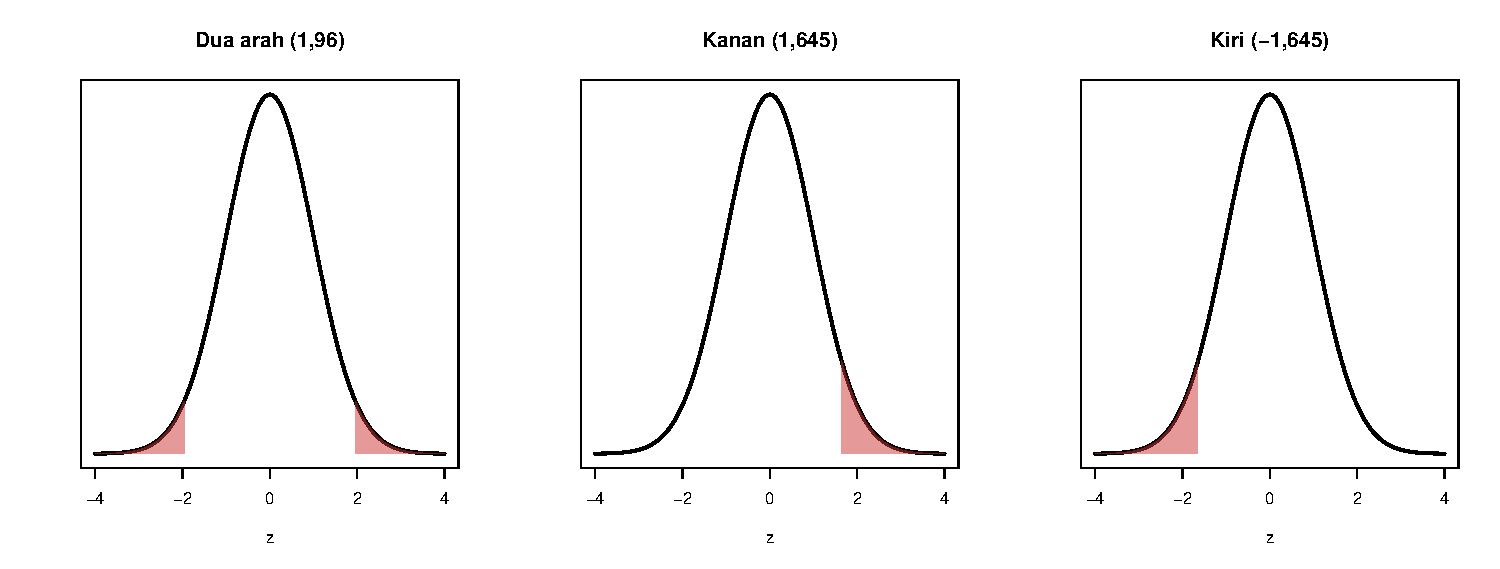
\includegraphics[keepaspectratio]{chapters/P10_files/figure-pdf/unnamed-chunk-4-1.pdf}}

\begin{Shaded}
\begin{Highlighting}[]
\FunctionTok{par}\NormalTok{(}\AttributeTok{mfrow =} \FunctionTok{c}\NormalTok{(}\DecValTok{1}\NormalTok{, }\DecValTok{1}\NormalTok{))}
\end{Highlighting}
\end{Shaded}

Daerah merah adalah daerah penolakan, luasnya \(\alpha = 0{,}05\). Pada
uji dua arah, \(\alpha\) dibagi dua ke kedua ekor.

\subsection{P-Value}\label{p-value}

\emph{P-value} adalah \textbf{peluang memperoleh statistik uji seekstrem
atau lebih ekstrem daripada yang teramati, dengan asumsi \(H_0\) benar}.

{\def\LTcaptype{none} % do not increment counter
\begin{longtable}[]{@{}ll@{}}
\toprule\noalign{}
Arah uji & P-value \\
\midrule\noalign{}
\endhead
\bottomrule\noalign{}
\endlastfoot
\textbf{Dua arah} & \(2 \times P(Z \ge |z|)\) \\
\textbf{Kanan} & \(P(Z \ge z)\) \\
\textbf{Kiri} & \(P(Z \le z)\) \\
\end{longtable}
}

\begin{Shaded}
\begin{Highlighting}[]
\NormalTok{p\_dua }\OtherTok{\textless{}{-}} \DecValTok{2} \SpecialCharTok{*}\NormalTok{ (}\DecValTok{1} \SpecialCharTok{{-}} \FunctionTok{pnorm}\NormalTok{(}\FunctionTok{abs}\NormalTok{(z\_hitung)))}
\NormalTok{p\_dua}
\end{Highlighting}
\end{Shaded}

\begin{verbatim}
[1] 0.01639507
\end{verbatim}

\begin{Shaded}
\begin{Highlighting}[]
\NormalTok{x }\OtherTok{\textless{}{-}} \FunctionTok{seq}\NormalTok{(}\SpecialCharTok{{-}}\DecValTok{4}\NormalTok{, }\DecValTok{4}\NormalTok{, }\AttributeTok{length.out =} \DecValTok{400}\NormalTok{)}
\FunctionTok{plot}\NormalTok{(x, }\FunctionTok{dnorm}\NormalTok{(x), }\AttributeTok{type =} \StringTok{"l"}\NormalTok{, }\AttributeTok{lwd =} \DecValTok{2}\NormalTok{, }\AttributeTok{xlab =} \StringTok{"z"}\NormalTok{, }\AttributeTok{ylab =} \StringTok{""}\NormalTok{, }\AttributeTok{yaxt =} \StringTok{"n"}\NormalTok{,}
     \AttributeTok{main =} \FunctionTok{paste0}\NormalTok{(}\StringTok{"P{-}value dua arah = luas kedua ekor = "}\NormalTok{, }\FunctionTok{round}\NormalTok{(p\_dua, }\DecValTok{4}\NormalTok{)))}
\ControlFlowTok{for}\NormalTok{ (bts }\ControlFlowTok{in} \FunctionTok{list}\NormalTok{(}\FunctionTok{c}\NormalTok{(}\SpecialCharTok{{-}}\DecValTok{4}\NormalTok{, }\SpecialCharTok{{-}}\FunctionTok{abs}\NormalTok{(z\_hitung)), }\FunctionTok{c}\NormalTok{(}\FunctionTok{abs}\NormalTok{(z\_hitung), }\DecValTok{4}\NormalTok{))) \{}
\NormalTok{  xs }\OtherTok{\textless{}{-}} \FunctionTok{seq}\NormalTok{(bts[}\DecValTok{1}\NormalTok{], bts[}\DecValTok{2}\NormalTok{], }\AttributeTok{length.out =} \DecValTok{100}\NormalTok{)}
  \FunctionTok{polygon}\NormalTok{(}\FunctionTok{c}\NormalTok{(bts[}\DecValTok{1}\NormalTok{], xs, bts[}\DecValTok{2}\NormalTok{]), }\FunctionTok{c}\NormalTok{(}\DecValTok{0}\NormalTok{, }\FunctionTok{dnorm}\NormalTok{(xs), }\DecValTok{0}\NormalTok{), }\AttributeTok{col =} \FunctionTok{rgb}\NormalTok{(}\FloatTok{0.2}\NormalTok{, }\FloatTok{0.4}\NormalTok{, }\FloatTok{0.8}\NormalTok{, }\FloatTok{0.5}\NormalTok{), }\AttributeTok{border =} \ConstantTok{NA}\NormalTok{)}
\NormalTok{\}}
\FunctionTok{abline}\NormalTok{(}\AttributeTok{v =} \FunctionTok{c}\NormalTok{(}\SpecialCharTok{{-}}\FloatTok{1.96}\NormalTok{, }\FloatTok{1.96}\NormalTok{), }\AttributeTok{lty =} \DecValTok{2}\NormalTok{, }\AttributeTok{col =} \StringTok{"firebrick"}\NormalTok{)}
\FunctionTok{text}\NormalTok{(z\_hitung, }\FloatTok{0.12}\NormalTok{, }\AttributeTok{labels =} \FunctionTok{paste0}\NormalTok{(}\StringTok{"z = "}\NormalTok{, }\FunctionTok{round}\NormalTok{(z\_hitung, }\DecValTok{2}\NormalTok{)), }\AttributeTok{pos =} \DecValTok{2}\NormalTok{)}
\end{Highlighting}
\end{Shaded}

\pandocbounded{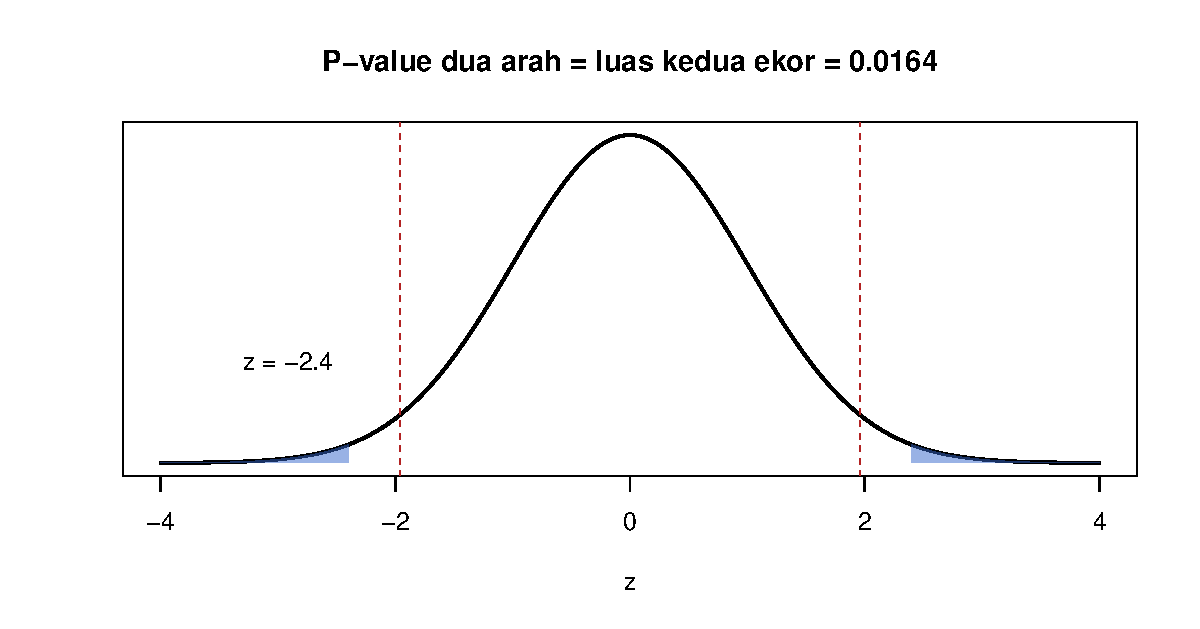
\includegraphics[keepaspectratio]{chapters/P10_files/figure-pdf/unnamed-chunk-5-1.pdf}}

\subsection{Keputusan: Dua Pendekatan yang
Setara}\label{keputusan-dua-pendekatan-yang-setara}

{\def\LTcaptype{none} % do not increment counter
\begin{longtable}[]{@{}
  >{\raggedright\arraybackslash}p{(\linewidth - 4\tabcolsep) * \real{0.3333}}
  >{\raggedright\arraybackslash}p{(\linewidth - 4\tabcolsep) * \real{0.3333}}
  >{\raggedright\arraybackslash}p{(\linewidth - 4\tabcolsep) * \real{0.3333}}@{}}
\toprule\noalign{}
\begin{minipage}[b]{\linewidth}\raggedright
Pendekatan
\end{minipage} & \begin{minipage}[b]{\linewidth}\raggedright
Tolak \(H_0\) jika
\end{minipage} & \begin{minipage}[b]{\linewidth}\raggedright
Contoh mesin kopi
\end{minipage} \\
\midrule\noalign{}
\endhead
\bottomrule\noalign{}
\endlastfoot
\textbf{Nilai kritis} & Statistik uji jatuh di daerah penolakan &
\(|z| = 2{,}4 > 1{,}96 \Rightarrow \text{tolak}\) \\
\textbf{P-value} & \(\text{p-value} \le \alpha\) &
\(0{,}0164 \le 0{,}05 \Rightarrow \text{tolak}\) \\
\end{longtable}
}

Kedua pendekatan selalu memberi keputusan yang sama. Pendekatan
\emph{p-value} lebih informatif karena menunjukkan seberapa kuat
buktinya, bukan sekadar lolos atau tidak.

{\def\LTcaptype{none} % do not increment counter
\begin{longtable}[]{@{}ll@{}}
\toprule\noalign{}
P-value & Kekuatan bukti melawan \(H_0\) (pedoman kasar) \\
\midrule\noalign{}
\endhead
\bottomrule\noalign{}
\endlastfoot
\(> 0{,}10\) & Lemah/tidak ada \\
\(0{,}05\text{–}0{,}10\) & Lemah-sedang \\
\(0{,}01\text{–}0{,}05\) & Cukup kuat \\
\(< 0{,}01\) & Sangat kuat \\
\end{longtable}
}

\begin{quote}
\textbf{``Gagal menolak \(H_0\)'' tidak sama dengan ``\(H_0\) benar''.}
Sama seperti ``tidak terbukti bersalah'' tidak berarti ``terbukti tidak
bersalah''. Bisa jadi efeknya memang ada tetapi sampel kita terlalu
kecil untuk mendeteksinya.
\end{quote}

\section{Prosedur Lima Langkah}\label{prosedur-lima-langkah}

{\def\LTcaptype{none} % do not increment counter
\begin{longtable}[]{@{}
  >{\raggedright\arraybackslash}p{(\linewidth - 2\tabcolsep) * \real{0.5000}}
  >{\raggedright\arraybackslash}p{(\linewidth - 2\tabcolsep) * \real{0.5000}}@{}}
\toprule\noalign{}
\begin{minipage}[b]{\linewidth}\raggedright
Langkah
\end{minipage} & \begin{minipage}[b]{\linewidth}\raggedright
Isi
\end{minipage} \\
\midrule\noalign{}
\endhead
\bottomrule\noalign{}
\endlastfoot
\textbf{1} & Rumuskan \(H_0\) dan \(H_1\) (tentukan arah) \\
\textbf{2} & Tetapkan \(\alpha\) \\
\textbf{3} & Pilih uji yang sesuai, periksa asumsi, hitung statistik
uji \\
\textbf{4} & Tentukan nilai kritis dan/atau \emph{p-value}, ambil
keputusan \\
\textbf{5} & Tulis kesimpulan dalam konteks masalah (bukan sekadar
``tolak \(H_0\)'') \\
\end{longtable}
}

Kita bungkus perhitungan uji \(z\) satu sampel dalam sebuah fungsi agar
dapat dipakai ulang.

\begin{Shaded}
\begin{Highlighting}[]
\NormalTok{uji\_z }\OtherTok{\textless{}{-}} \ControlFlowTok{function}\NormalTok{(xbar, mu0, sigma, n, }\AttributeTok{arah =} \FunctionTok{c}\NormalTok{(}\StringTok{"dua"}\NormalTok{, }\StringTok{"kanan"}\NormalTok{, }\StringTok{"kiri"}\NormalTok{), }\AttributeTok{alpha =} \FloatTok{0.05}\NormalTok{) \{}
\NormalTok{  arah }\OtherTok{\textless{}{-}} \FunctionTok{match.arg}\NormalTok{(arah)}
\NormalTok{  z }\OtherTok{\textless{}{-}}\NormalTok{ (xbar }\SpecialCharTok{{-}}\NormalTok{ mu0) }\SpecialCharTok{/}\NormalTok{ (sigma }\SpecialCharTok{/} \FunctionTok{sqrt}\NormalTok{(n))}
\NormalTok{  p }\OtherTok{\textless{}{-}} \ControlFlowTok{switch}\NormalTok{(arah,}
              \AttributeTok{dua =} \DecValTok{2} \SpecialCharTok{*}\NormalTok{ (}\DecValTok{1} \SpecialCharTok{{-}} \FunctionTok{pnorm}\NormalTok{(}\FunctionTok{abs}\NormalTok{(z))),}
              \AttributeTok{kanan =} \DecValTok{1} \SpecialCharTok{{-}} \FunctionTok{pnorm}\NormalTok{(z),}
              \AttributeTok{kiri =} \FunctionTok{pnorm}\NormalTok{(z))}
\NormalTok{  kritis }\OtherTok{\textless{}{-}} \ControlFlowTok{switch}\NormalTok{(arah,}
                   \AttributeTok{dua =} \FunctionTok{qnorm}\NormalTok{(}\DecValTok{1} \SpecialCharTok{{-}}\NormalTok{ alpha }\SpecialCharTok{/} \DecValTok{2}\NormalTok{),}
                   \AttributeTok{kanan =} \FunctionTok{qnorm}\NormalTok{(}\DecValTok{1} \SpecialCharTok{{-}}\NormalTok{ alpha),}
                   \AttributeTok{kiri =} \FunctionTok{qnorm}\NormalTok{(alpha))}
  \FunctionTok{data.frame}\NormalTok{(}\AttributeTok{z =} \FunctionTok{round}\NormalTok{(z, }\DecValTok{4}\NormalTok{),}
             \AttributeTok{z\_kritis =} \FunctionTok{round}\NormalTok{(kritis, }\DecValTok{4}\NormalTok{),}
             \AttributeTok{p\_value =} \FunctionTok{signif}\NormalTok{(p, }\DecValTok{4}\NormalTok{),}
             \AttributeTok{keputusan =} \FunctionTok{ifelse}\NormalTok{(p }\SpecialCharTok{\textless{}=}\NormalTok{ alpha, }\StringTok{"Tolak H0"}\NormalTok{, }\StringTok{"Gagal menolak H0"}\NormalTok{))}
\NormalTok{\}}
\end{Highlighting}
\end{Shaded}

\subsection{Contoh 1 (Dua Arah): Mesin Pengisi
Kopi}\label{contoh-1-dua-arah-mesin-pengisi-kopi}

\begin{enumerate}
\def\labelenumi{\arabic{enumi}.}
\tightlist
\item
  \(H_0: \mu = 250\) gram (mesin tepat); \(H_1: \mu \ne 250\) gram
  (mesin perlu dikalibrasi).
\item
  \(\alpha = 0{,}05\).
\item
  \(\sigma\) diketahui (\(6\) g), \(n = 36 \Rightarrow\) uji \(z\):
  \(z = (247{,}6 - 250) / 1 = -2{,}4\).
\end{enumerate}

\begin{Shaded}
\begin{Highlighting}[]
\FunctionTok{uji\_z}\NormalTok{(}\AttributeTok{xbar =} \FloatTok{247.6}\NormalTok{, }\AttributeTok{mu0 =} \DecValTok{250}\NormalTok{, }\AttributeTok{sigma =} \DecValTok{6}\NormalTok{, }\AttributeTok{n =} \DecValTok{36}\NormalTok{, }\AttributeTok{arah =} \StringTok{"dua"}\NormalTok{)}
\end{Highlighting}
\end{Shaded}

\begin{verbatim}
     z z_kritis p_value keputusan
1 -2.4     1.96  0.0164  Tolak H0
\end{verbatim}

\begin{enumerate}
\def\labelenumi{\arabic{enumi}.}
\setcounter{enumi}{3}
\tightlist
\item
  \(|z| = 2{,}4 > 1{,}96\) dan
  \(\text{p-value} \approx 0{,}016 < 0{,}05 \Rightarrow\) \textbf{tolak
  \(H_0\)}.
\item
  \textbf{Kesimpulan:} Pada taraf signifikansi \(5\%\), terdapat bukti
  yang cukup bahwa rata-rata pengisian mesin berbeda dari \(250\) gram
  (data menunjukkan cenderung kurang). Mesin sebaiknya diperiksa dan
  dikalibrasi.
\end{enumerate}

\subsection{Contoh 2 (Satu Arah Kanan): Klaim Waktu
Pengiriman}\label{contoh-2-satu-arah-kanan-klaim-waktu-pengiriman}

Sebuah layanan logistik mengklaim rata-rata waktu pengirimannya paling
lama \(48\) jam. Asosiasi konsumen curiga waktunya lebih lama. Data
historis menunjukkan \(\sigma = 10\) jam. Sampel \(50\) pengiriman
menghasilkan \(\bar{x} = 50{,}1\) jam.

\begin{enumerate}
\def\labelenumi{\arabic{enumi}.}
\tightlist
\item
  \(H_0: \mu \le 48\) (klaim benar); \(H_1: \mu > 48\) (klaim tidak
  benar --- lebih lama).
\item
  \(\alpha = 0{,}05\).
\end{enumerate}

\begin{Shaded}
\begin{Highlighting}[]
\FunctionTok{uji\_z}\NormalTok{(}\AttributeTok{xbar =} \FloatTok{50.1}\NormalTok{, }\AttributeTok{mu0 =} \DecValTok{48}\NormalTok{, }\AttributeTok{sigma =} \DecValTok{10}\NormalTok{, }\AttributeTok{n =} \DecValTok{50}\NormalTok{, }\AttributeTok{arah =} \StringTok{"kanan"}\NormalTok{)}
\end{Highlighting}
\end{Shaded}

\begin{verbatim}
       z z_kritis p_value        keputusan
1 1.4849   1.6449 0.06878 Gagal menolak H0
\end{verbatim}

\begin{enumerate}
\def\labelenumi{\arabic{enumi}.}
\setcounter{enumi}{2}
\tightlist
\item
  \textbf{Kesimpulan:} \(\text{p-value} \approx 0{,}069 > 0{,}05\),
  sehingga \textbf{gagal menolak \(H_0\)}. Pada taraf \(5\%\), bukti
  belum cukup untuk menyatakan rata-rata waktu pengiriman melebihi
  \(48\) jam. Ini tidak membuktikan klaim perusahaan benar; dengan
  \emph{p-value} \(0{,}07\), ada indikasi lemah yang layak
  ditindaklanjuti dengan sampel lebih besar.
\end{enumerate}

\begin{quote}
\textbf{Perhatikan:} Jika asosiasi konsumen memakai uji dua arah,
\emph{p-value}-nya menjadi dua kali lipat (sekitar \(0{,}14\)). Arah uji
harus ditentukan dari pertanyaan penelitian sebelum melihat data.
\end{quote}

\section{Hubungan Uji Dua Arah dan Selang
Kepercayaan}\label{hubungan-uji-dua-arah-dan-selang-kepercayaan}

Uji dua arah dengan taraf \(\alpha\) setara dengan memeriksa apakah
\(\mu_0\) berada di dalam selang kepercayaan
\((1 - \alpha) \times 100\%\):

\begin{itemize}
\tightlist
\item
  \(\mu_0\) di luar CI 95\% \(\iff\) tolak \(H_0\) pada
  \(\alpha = 0{,}05\) (dua arah).
\item
  \(\mu_0\) di dalam CI 95\% \(\iff\) gagal menolak \(H_0\).
\end{itemize}

\begin{Shaded}
\begin{Highlighting}[]
\NormalTok{ci }\OtherTok{\textless{}{-}} \FloatTok{247.6} \SpecialCharTok{+} \FunctionTok{c}\NormalTok{(}\SpecialCharTok{{-}}\DecValTok{1}\NormalTok{, }\DecValTok{1}\NormalTok{) }\SpecialCharTok{*} \FunctionTok{qnorm}\NormalTok{(}\FloatTok{0.975}\NormalTok{) }\SpecialCharTok{*} \DecValTok{6} \SpecialCharTok{/} \FunctionTok{sqrt}\NormalTok{(}\DecValTok{36}\NormalTok{)}
\FunctionTok{round}\NormalTok{(ci, }\DecValTok{3}\NormalTok{)}
\end{Highlighting}
\end{Shaded}

\begin{verbatim}
[1] 245.64 249.56
\end{verbatim}

\begin{Shaded}
\begin{Highlighting}[]
\DecValTok{250} \SpecialCharTok{\textgreater{}=}\NormalTok{ ci[}\DecValTok{1}\NormalTok{] }\SpecialCharTok{\&} \DecValTok{250} \SpecialCharTok{\textless{}=}\NormalTok{ ci[}\DecValTok{2}\NormalTok{] }\CommentTok{\# FALSE {-}\textgreater{} 250 di luar selang {-}\textgreater{} konsisten dengan "tolak H0"}
\end{Highlighting}
\end{Shaded}

\begin{verbatim}
[1] FALSE
\end{verbatim}

Selang kepercayaan lebih informatif: selain keputusan, ia menunjukkan
rentang nilai \(\mu\) yang masuk akal --- di sini rata-rata pengisian
kemungkinan antara \(245{,}6\) dan \(249{,}6\) gram, sehingga
kekurangannya kemungkinan antara \(0{,}4\) dan \(4{,}4\) gram per
kemasan.

\section{Kesalahan Tipe I, Tipe II, dan
Power}\label{kesalahan-tipe-i-tipe-ii-dan-power}

\subsection{Tabel Keputusan}\label{tabel-keputusan}

{\def\LTcaptype{none} % do not increment counter
\begin{longtable}[]{@{}
  >{\raggedright\arraybackslash}p{(\linewidth - 4\tabcolsep) * \real{0.3333}}
  >{\raggedright\arraybackslash}p{(\linewidth - 4\tabcolsep) * \real{0.3333}}
  >{\raggedright\arraybackslash}p{(\linewidth - 4\tabcolsep) * \real{0.3333}}@{}}
\toprule\noalign{}
\begin{minipage}[b]{\linewidth}\raggedright
Keputusan
\end{minipage} & \begin{minipage}[b]{\linewidth}\raggedright
\(H_0\) benar
\end{minipage} & \begin{minipage}[b]{\linewidth}\raggedright
\(H_0\) salah
\end{minipage} \\
\midrule\noalign{}
\endhead
\bottomrule\noalign{}
\endlastfoot
\textbf{Tolak \(H_0\)} & Kesalahan Tipe I (\emph{false positive}),
peluang \(= \alpha\) & Keputusan benar, peluang
\(= \text{power} = 1 - \beta\) \\
\textbf{Gagal menolak \(H_0\)} & Keputusan benar, peluang
\(= 1 - \alpha\) & Kesalahan Tipe II (\emph{false negative}), peluang
\(= \beta\) \\
\end{longtable}
}

{\def\LTcaptype{none} % do not increment counter
\begin{longtable}[]{@{}
  >{\raggedright\arraybackslash}p{(\linewidth - 4\tabcolsep) * \real{0.3333}}
  >{\raggedright\arraybackslash}p{(\linewidth - 4\tabcolsep) * \real{0.3333}}
  >{\raggedright\arraybackslash}p{(\linewidth - 4\tabcolsep) * \real{0.3333}}@{}}
\toprule\noalign{}
\begin{minipage}[b]{\linewidth}\raggedright
Konteks
\end{minipage} & \begin{minipage}[b]{\linewidth}\raggedright
Kesalahan Tipe I
\end{minipage} & \begin{minipage}[b]{\linewidth}\raggedright
Kesalahan Tipe II
\end{minipage} \\
\midrule\noalign{}
\endhead
\bottomrule\noalign{}
\endlastfoot
\textbf{Mesin pengisi} (\(H_0\): mesin tepat) & Menghentikan produksi
untuk kalibrasi padahal mesin baik & Mesin terus mengisi kurang;
konsumen dirugikan \\
\textbf{Tes penyakit} (\(H_0\): sehat) & Orang sehat didiagnosis sakit &
Orang sakit tidak terdeteksi \\
\textbf{Filter spam} (\(H_0\): bukan spam) & Email penting masuk folder
spam & Spam lolos ke kotak masuk \\
\textbf{Uji A/B} (\(H_0\): desain baru tidak lebih baik) & Meluncurkan
desain yang sebenarnya tidak lebih baik & Melewatkan desain yang
sebenarnya lebih baik \\
\end{longtable}
}

\subsection{\texorpdfstring{Simulasi: Kesalahan Tipe I Terjadi Sekitar
\(\alpha\) dari
Waktu}{Simulasi: Kesalahan Tipe I Terjadi Sekitar \textbackslash alpha dari Waktu}}\label{simulasi-kesalahan-tipe-i-terjadi-sekitar-alpha-dari-waktu}

Jika mesin benar-benar tepat (\(\mu = 250\)) dan kita menguji \(10.000\)
sampel berbeda, berapa kali kita keliru menolak \(H_0\)?

\begin{Shaded}
\begin{Highlighting}[]
\FunctionTok{set.seed}\NormalTok{(}\DecValTok{101}\NormalTok{)}
\NormalTok{p\_values\_H0 }\OtherTok{\textless{}{-}} \FunctionTok{replicate}\NormalTok{(}\DecValTok{10000}\NormalTok{, \{}
\NormalTok{  x }\OtherTok{\textless{}{-}} \FunctionTok{rnorm}\NormalTok{(}\DecValTok{36}\NormalTok{, }\AttributeTok{mean =} \DecValTok{250}\NormalTok{, }\AttributeTok{sd =} \DecValTok{6}\NormalTok{)}
\NormalTok{  z }\OtherTok{\textless{}{-}}\NormalTok{ (}\FunctionTok{mean}\NormalTok{(x) }\SpecialCharTok{{-}} \DecValTok{250}\NormalTok{) }\SpecialCharTok{/}\NormalTok{ (}\DecValTok{6} \SpecialCharTok{/} \DecValTok{6}\NormalTok{)}
  \DecValTok{2} \SpecialCharTok{*}\NormalTok{ (}\DecValTok{1} \SpecialCharTok{{-}} \FunctionTok{pnorm}\NormalTok{(}\FunctionTok{abs}\NormalTok{(z)))}
\NormalTok{\})}

\FunctionTok{mean}\NormalTok{(p\_values\_H0 }\SpecialCharTok{\textless{}=} \FloatTok{0.05}\NormalTok{) }\CommentTok{\# proporsi kesalahan Tipe I}
\end{Highlighting}
\end{Shaded}

\begin{verbatim}
[1] 0.0482
\end{verbatim}

\begin{Shaded}
\begin{Highlighting}[]
\FunctionTok{hist}\NormalTok{(p\_values\_H0, }\AttributeTok{breaks =} \DecValTok{20}\NormalTok{, }\AttributeTok{col =} \StringTok{"\#c6dbef"}\NormalTok{, }\AttributeTok{border =} \StringTok{"white"}\NormalTok{,}
     \AttributeTok{main =} \StringTok{"Distribusi p{-}value ketika H0 BENAR: seragam"}\NormalTok{,}
     \AttributeTok{xlab =} \StringTok{"p{-}value"}\NormalTok{, }\AttributeTok{ylab =} \StringTok{"Frekuensi"}\NormalTok{)}
\FunctionTok{abline}\NormalTok{(}\AttributeTok{v =} \FloatTok{0.05}\NormalTok{, }\AttributeTok{col =} \StringTok{"firebrick"}\NormalTok{, }\AttributeTok{lwd =} \DecValTok{2}\NormalTok{)}
\end{Highlighting}
\end{Shaded}

\pandocbounded{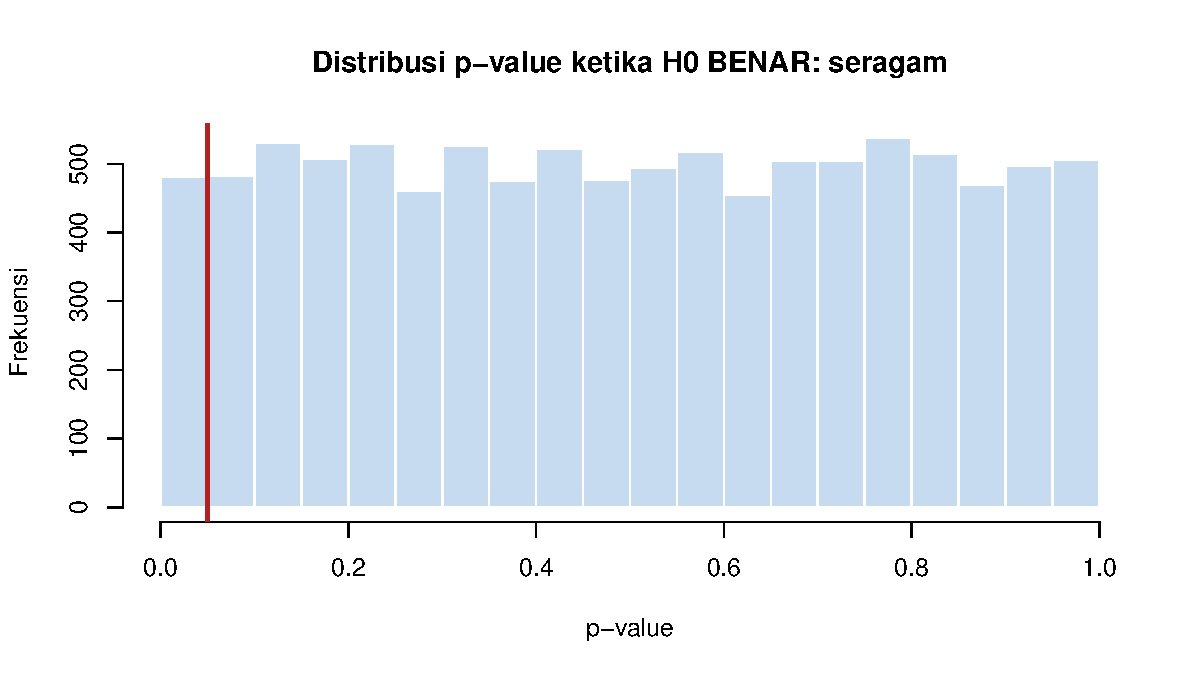
\includegraphics[keepaspectratio]{chapters/P10_files/figure-pdf/unnamed-chunk-10-1.pdf}}

Ketika \(H_0\) benar, \emph{p-value} tersebar merata antara \(0\) dan
\(1\); sekitar \(5\%\) di antaranya jatuh di bawah \(0{,}05\) murni
karena kebetulan. Itulah makna \(\alpha\).

\subsection{Simulasi: Kesalahan Tipe II dan
Power}\label{simulasi-kesalahan-tipe-ii-dan-power}

Sekarang anggap mesin benar-benar mengisi rata-rata \(248\) gram
(\(H_0\) salah). Seberapa sering uji kita mendeteksinya?

\begin{Shaded}
\begin{Highlighting}[]
\NormalTok{power\_sim }\OtherTok{\textless{}{-}} \ControlFlowTok{function}\NormalTok{(mu\_benar, n, }\AttributeTok{alpha =} \FloatTok{0.05}\NormalTok{, }\AttributeTok{B =} \DecValTok{5000}\NormalTok{) \{}
  \FunctionTok{mean}\NormalTok{(}\FunctionTok{replicate}\NormalTok{(B, \{}
\NormalTok{    z }\OtherTok{\textless{}{-}}\NormalTok{ (}\FunctionTok{mean}\NormalTok{(}\FunctionTok{rnorm}\NormalTok{(n, mu\_benar, }\DecValTok{6}\NormalTok{)) }\SpecialCharTok{{-}} \DecValTok{250}\NormalTok{) }\SpecialCharTok{/}\NormalTok{ (}\DecValTok{6} \SpecialCharTok{/} \FunctionTok{sqrt}\NormalTok{(n))}
    \DecValTok{2} \SpecialCharTok{*}\NormalTok{ (}\DecValTok{1} \SpecialCharTok{{-}} \FunctionTok{pnorm}\NormalTok{(}\FunctionTok{abs}\NormalTok{(z))) }\SpecialCharTok{\textless{}=}\NormalTok{ alpha}
\NormalTok{  \}))}
\NormalTok{\}}

\NormalTok{power\_teori }\OtherTok{\textless{}{-}} \ControlFlowTok{function}\NormalTok{(mu\_benar, n, }\AttributeTok{alpha =} \FloatTok{0.05}\NormalTok{) \{}
\NormalTok{  k }\OtherTok{\textless{}{-}} \FunctionTok{qnorm}\NormalTok{(}\DecValTok{1} \SpecialCharTok{{-}}\NormalTok{ alpha }\SpecialCharTok{/} \DecValTok{2}\NormalTok{)}
\NormalTok{  d }\OtherTok{\textless{}{-}}\NormalTok{ (mu\_benar }\SpecialCharTok{{-}} \DecValTok{250}\NormalTok{) }\SpecialCharTok{/}\NormalTok{ (}\DecValTok{6} \SpecialCharTok{/} \FunctionTok{sqrt}\NormalTok{(n))}
  \FunctionTok{pnorm}\NormalTok{(}\SpecialCharTok{{-}}\NormalTok{k }\SpecialCharTok{{-}}\NormalTok{ d) }\SpecialCharTok{+} \DecValTok{1} \SpecialCharTok{{-}} \FunctionTok{pnorm}\NormalTok{(k }\SpecialCharTok{{-}}\NormalTok{ d)}
\NormalTok{\}}

\FunctionTok{set.seed}\NormalTok{(}\DecValTok{102}\NormalTok{)}
\FunctionTok{c}\NormalTok{(}\AttributeTok{Power\_simulasi =} \FunctionTok{power\_sim}\NormalTok{(}\DecValTok{248}\NormalTok{, }\DecValTok{36}\NormalTok{),}
  \AttributeTok{Power\_teori =} \FunctionTok{round}\NormalTok{(}\FunctionTok{power\_teori}\NormalTok{(}\DecValTok{248}\NormalTok{, }\DecValTok{36}\NormalTok{), }\DecValTok{4}\NormalTok{),}
  \AttributeTok{Beta\_teori =} \FunctionTok{round}\NormalTok{(}\DecValTok{1} \SpecialCharTok{{-}} \FunctionTok{power\_teori}\NormalTok{(}\DecValTok{248}\NormalTok{, }\DecValTok{36}\NormalTok{), }\DecValTok{4}\NormalTok{))}
\end{Highlighting}
\end{Shaded}

\begin{verbatim}
Power_simulasi    Power_teori     Beta_teori 
        0.5078         0.5160         0.4840 
\end{verbatim}

Dengan \(n = 36\), uji hanya mendeteksi selisih \(2\) gram sekitar
\(52\%\) dari waktu; sekitar \(48\%\) dari waktu mesin yang salah setel
lolos (kesalahan Tipe II).

\subsection{Kurva Power: Faktor yang
Memengaruhi}\label{kurva-power-faktor-yang-memengaruhi}

\begin{Shaded}
\begin{Highlighting}[]
\NormalTok{mu\_seq }\OtherTok{\textless{}{-}} \FunctionTok{seq}\NormalTok{(}\DecValTok{245}\NormalTok{, }\DecValTok{255}\NormalTok{, }\AttributeTok{by =} \FloatTok{0.05}\NormalTok{)}
\FunctionTok{plot}\NormalTok{(mu\_seq, }\FunctionTok{power\_teori}\NormalTok{(mu\_seq, }\DecValTok{36}\NormalTok{), }\AttributeTok{type =} \StringTok{"l"}\NormalTok{, }\AttributeTok{lwd =} \DecValTok{2}\NormalTok{, }\AttributeTok{col =} \StringTok{"\#4C72B0"}\NormalTok{, }\AttributeTok{ylim =} \FunctionTok{c}\NormalTok{(}\DecValTok{0}\NormalTok{, }\DecValTok{1}\NormalTok{),}
     \AttributeTok{xlab =} \StringTok{"Rata{-}rata pengisian sebenarnya (gram)"}\NormalTok{, }\AttributeTok{ylab =} \StringTok{"Power = P(tolak H0)"}\NormalTok{,}
     \AttributeTok{main =} \StringTok{"Kurva Power Uji Dua Arah (H0: mu = 250)"}\NormalTok{)}
\FunctionTok{lines}\NormalTok{(mu\_seq, }\FunctionTok{power\_teori}\NormalTok{(mu\_seq, }\DecValTok{100}\NormalTok{), }\AttributeTok{lwd =} \DecValTok{2}\NormalTok{, }\AttributeTok{col =} \StringTok{"\#DD8452"}\NormalTok{)}
\FunctionTok{lines}\NormalTok{(mu\_seq, }\FunctionTok{power\_teori}\NormalTok{(mu\_seq, }\DecValTok{36}\NormalTok{, }\AttributeTok{alpha =} \FloatTok{0.01}\NormalTok{), }\AttributeTok{lwd =} \DecValTok{2}\NormalTok{, }\AttributeTok{lty =} \DecValTok{2}\NormalTok{, }\AttributeTok{col =} \StringTok{"\#4C72B0"}\NormalTok{)}
\FunctionTok{abline}\NormalTok{(}\AttributeTok{h =} \FunctionTok{c}\NormalTok{(}\FloatTok{0.05}\NormalTok{, }\FloatTok{0.8}\NormalTok{), }\AttributeTok{lty =} \DecValTok{3}\NormalTok{, }\AttributeTok{col =} \StringTok{"grey50"}\NormalTok{)}
\FunctionTok{legend}\NormalTok{(}\StringTok{"top"}\NormalTok{, }\AttributeTok{bty =} \StringTok{"n"}\NormalTok{, }\AttributeTok{lwd =} \DecValTok{2}\NormalTok{, }\AttributeTok{lty =} \FunctionTok{c}\NormalTok{(}\DecValTok{1}\NormalTok{, }\DecValTok{1}\NormalTok{, }\DecValTok{2}\NormalTok{),}
       \AttributeTok{col =} \FunctionTok{c}\NormalTok{(}\StringTok{"\#4C72B0"}\NormalTok{, }\StringTok{"\#DD8452"}\NormalTok{, }\StringTok{"\#4C72B0"}\NormalTok{), }\AttributeTok{cex =} \FloatTok{0.8}\NormalTok{,}
       \AttributeTok{legend =} \FunctionTok{c}\NormalTok{(}\StringTok{"n = 36, alpha = 0,05"}\NormalTok{, }\StringTok{"n = 100, alpha = 0,05"}\NormalTok{, }\StringTok{"n = 36, alpha = 0,01"}\NormalTok{))}
\end{Highlighting}
\end{Shaded}

\pandocbounded{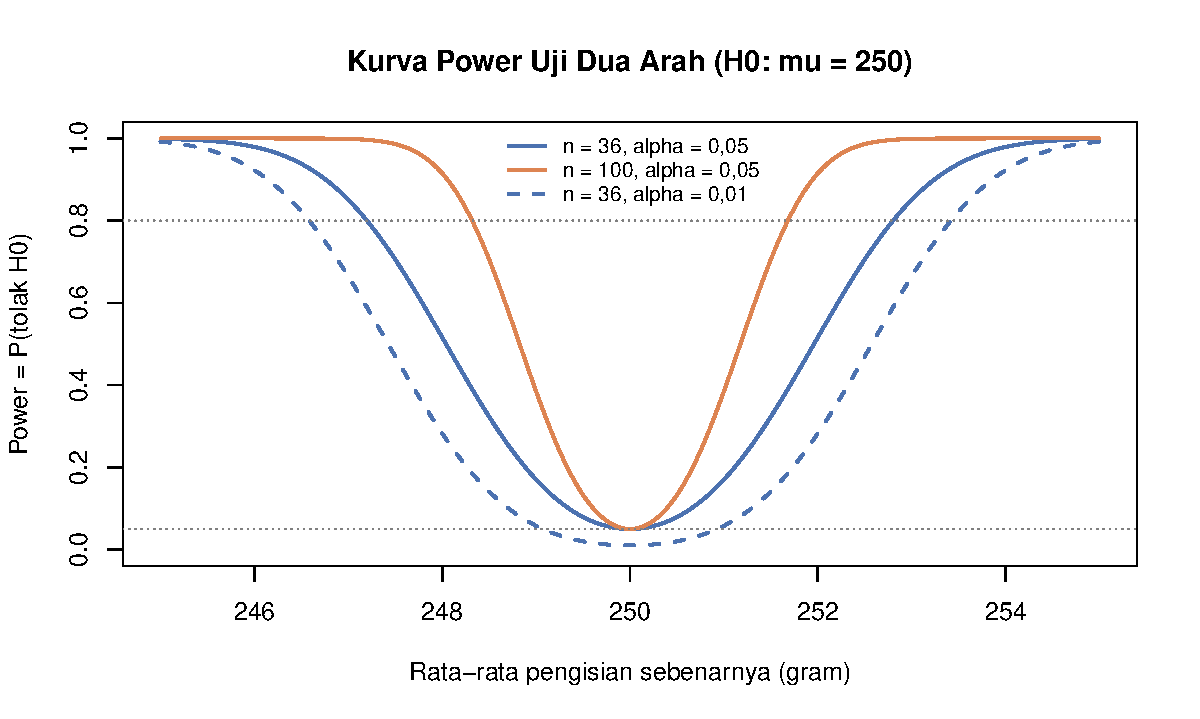
\includegraphics[keepaspectratio]{chapters/P10_files/figure-pdf/unnamed-chunk-12-1.pdf}}

{\def\LTcaptype{none} % do not increment counter
\begin{longtable}[]{@{}
  >{\raggedright\arraybackslash}p{(\linewidth - 4\tabcolsep) * \real{0.3333}}
  >{\raggedright\arraybackslash}p{(\linewidth - 4\tabcolsep) * \real{0.3333}}
  >{\raggedright\arraybackslash}p{(\linewidth - 4\tabcolsep) * \real{0.3333}}@{}}
\toprule\noalign{}
\begin{minipage}[b]{\linewidth}\raggedright
Faktor
\end{minipage} & \begin{minipage}[b]{\linewidth}\raggedright
Jika dinaikkan
\end{minipage} & \begin{minipage}[b]{\linewidth}\raggedright
Power
\end{minipage} \\
\midrule\noalign{}
\endhead
\bottomrule\noalign{}
\endlastfoot
\textbf{Besar efek sebenarnya} (\(|\mu - \mu_0|\)) & Selisih makin besar
& \textbf{Naik} \\
\textbf{Ukuran sampel} (\(n\)) & \(SE\) mengecil & \textbf{Naik} \\
\textbf{Tingkat signifikansi} (\(\alpha\)) & Daerah penolakan melebar &
\textbf{Naik} (tetapi risiko Tipe I naik) \\
\textbf{Variabilitas} (\(\sigma\)) & \(SE\) membesar & \textbf{Turun} \\
\end{longtable}
}

Tepat di \(\mu = 250\) (saat \(H_0\) benar), kurva menyentuh
\(0{,}05 = \alpha\). \emph{Trade-off}: memperkecil \(\alpha\) (garis
putus-putus) mengurangi kesalahan Tipe I tetapi menurunkan \emph{power}
(menambah kesalahan Tipe II). Satu-satunya cara mengurangi keduanya
sekaligus adalah memperbesar sampel.

Konvensi yang umum dipakai: rancang studi agar \emph{power} minimal
\(0{,}80\) untuk efek terkecil yang dianggap penting.

\begin{Shaded}
\begin{Highlighting}[]
\NormalTok{n\_power }\OtherTok{\textless{}{-}} \ControlFlowTok{function}\NormalTok{(delta, sigma, }\AttributeTok{alpha =} \FloatTok{0.05}\NormalTok{, }\AttributeTok{power =} \FloatTok{0.80}\NormalTok{) \{}
  \FunctionTok{ceiling}\NormalTok{(((}\FunctionTok{qnorm}\NormalTok{(}\DecValTok{1} \SpecialCharTok{{-}}\NormalTok{ alpha }\SpecialCharTok{/} \DecValTok{2}\NormalTok{) }\SpecialCharTok{+} \FunctionTok{qnorm}\NormalTok{(power)) }\SpecialCharTok{*}\NormalTok{ sigma }\SpecialCharTok{/}\NormalTok{ delta)}\SpecialCharTok{\^{}}\DecValTok{2}\NormalTok{)}
\NormalTok{\}}

\FunctionTok{n\_power}\NormalTok{(}\AttributeTok{delta =} \DecValTok{2}\NormalTok{, }\AttributeTok{sigma =} \DecValTok{6}\NormalTok{) }\CommentTok{\# sampel agar selisih 2 gram terdeteksi dengan power 80\%}
\end{Highlighting}
\end{Shaded}

\begin{verbatim}
[1] 71
\end{verbatim}

\section{Menafsirkan Hasil Uji dengan
Bijak}\label{menafsirkan-hasil-uji-dengan-bijak}

\subsection{Signifikansi Statistik vs Signifikansi
Praktis}\label{signifikansi-statistik-vs-signifikansi-praktis}

Dengan sampel sangat besar, selisih yang sangat kecil pun menjadi
``signifikan secara statistik''.

\begin{Shaded}
\begin{Highlighting}[]
\NormalTok{knitr}\SpecialCharTok{::}\FunctionTok{kable}\NormalTok{(}\FunctionTok{rbind}\NormalTok{(}
  \StringTok{"n = 36"} \OtherTok{=} \FunctionTok{uji\_z}\NormalTok{(}\AttributeTok{xbar =} \FloatTok{249.8}\NormalTok{, }\AttributeTok{mu0 =} \DecValTok{250}\NormalTok{, }\AttributeTok{sigma =} \DecValTok{6}\NormalTok{, }\AttributeTok{n =} \DecValTok{36}\NormalTok{),}
  \StringTok{"n = 100.000"} \OtherTok{=} \FunctionTok{uji\_z}\NormalTok{(}\AttributeTok{xbar =} \FloatTok{249.8}\NormalTok{, }\AttributeTok{mu0 =} \DecValTok{250}\NormalTok{, }\AttributeTok{sigma =} \DecValTok{6}\NormalTok{, }\AttributeTok{n =} \DecValTok{100000}\NormalTok{)}
\NormalTok{), }\AttributeTok{caption =} \StringTok{"Selisih 0,2 gram: tidak signifikan vs sangat signifikan"}\NormalTok{)}
\end{Highlighting}
\end{Shaded}

\begin{longtable}[]{@{}lrrrl@{}}
\caption{Selisih 0,2 gram: tidak signifikan vs sangat
signifikan}\tabularnewline
\toprule\noalign{}
& z & z\_kritis & p\_value & keputusan \\
\midrule\noalign{}
\endfirsthead
\toprule\noalign{}
& z & z\_kritis & p\_value & keputusan \\
\midrule\noalign{}
\endhead
\bottomrule\noalign{}
\endlastfoot
n = 36 & -0.2000 & 1.96 & 0.8415 & Gagal menolak H0 \\
n = 100.000 & -10.5409 & 1.96 & 0.0000 & Tolak H0 \\
\end{longtable}

Selisih \(0{,}2\) gram per kemasan (\(0{,}08\%\)) kemungkinan tidak
penting secara praktis, meskipun signifikan secara statistik pada
\(n = 100.000\). Karena itu, selalu laporkan besar efek (selisih dan
selang kepercayaannya), bukan hanya \emph{p-value}.

\subsection{Miskonsepsi tentang
P-Value}\label{miskonsepsi-tentang-p-value}

{\def\LTcaptype{none} % do not increment counter
\begin{longtable}[]{@{}
  >{\raggedright\arraybackslash}p{(\linewidth - 4\tabcolsep) * \real{0.3333}}
  >{\raggedright\arraybackslash}p{(\linewidth - 4\tabcolsep) * \real{0.3333}}
  >{\raggedright\arraybackslash}p{(\linewidth - 4\tabcolsep) * \real{0.3333}}@{}}
\toprule\noalign{}
\begin{minipage}[b]{\linewidth}\raggedright
Pernyataan
\end{minipage} & \begin{minipage}[b]{\linewidth}\raggedright
Benar/Salah
\end{minipage} & \begin{minipage}[b]{\linewidth}\raggedright
Penjelasan
\end{minipage} \\
\midrule\noalign{}
\endhead
\bottomrule\noalign{}
\endlastfoot
``\(p = 0{,}016\) berarti peluang \(H_0\) benar adalah \(1{,}6\%\).'' &
\textbf{Salah} & \emph{P-value} dihitung dengan asumsi \(H_0\) benar; ia
bukan peluang \(H_0\) benar \\
``\(p = 0{,}016\) berarti peluang hasil ini terjadi karena kebetulan
adalah \(1{,}6\%\).'' & \textbf{Salah} & Sama dengan di atas, dengan
kata-kata berbeda \\
``\(p > 0{,}05\) membuktikan tidak ada efek.'' & \textbf{Salah} & Bisa
jadi \emph{power} rendah (sampel kecil) \\
``\emph{P} yang lebih kecil berarti efeknya lebih besar.'' &
\textbf{Salah} & \emph{P-value} dipengaruhi besar efek dan ukuran
sampel \\
``\(p = 0{,}049\) dan \(p = 0{,}051\) memberi bukti yang sangat
berbeda.'' & \textbf{Salah} & Keduanya menunjukkan kekuatan bukti yang
hampir sama \\
``Jika \(H_0\) benar, \emph{p-value} kurang dari \(0{,}05\) terjadi
sekitar \(5\%\) dari waktu.'' & \textbf{Benar} & Inilah makna
\(\alpha\) \\
\end{longtable}
}

\subsection{Bahaya Uji Berganda
(P-Hacking)}\label{bahaya-uji-berganda-p-hacking}

Jika kita menguji banyak hipotesis sekaligus --- atau mencoba banyak
cara analisis sampai ada yang ``signifikan'' --- peluang setidaknya satu
kesalahan Tipe I melonjak.

\begin{Shaded}
\begin{Highlighting}[]
\NormalTok{k }\OtherTok{\textless{}{-}} \FunctionTok{c}\NormalTok{(}\DecValTok{1}\NormalTok{, }\DecValTok{5}\NormalTok{, }\DecValTok{10}\NormalTok{, }\DecValTok{20}\NormalTok{, }\DecValTok{50}\NormalTok{)}
\FunctionTok{data.frame}\NormalTok{(}\AttributeTok{Banyak\_uji =}\NormalTok{ k, }\AttributeTok{P\_minimal\_satu\_false\_positive =} \FunctionTok{round}\NormalTok{(}\DecValTok{1} \SpecialCharTok{{-}}\NormalTok{ (}\DecValTok{1} \SpecialCharTok{{-}} \FloatTok{0.05}\NormalTok{)}\SpecialCharTok{\^{}}\NormalTok{k, }\DecValTok{3}\NormalTok{))}
\end{Highlighting}
\end{Shaded}

\begin{verbatim}
  Banyak_uji P_minimal_satu_false_positive
1          1                         0.050
2          5                         0.226
3         10                         0.401
4         20                         0.642
5         50                         0.923
\end{verbatim}

\begin{Shaded}
\begin{Highlighting}[]
\FunctionTok{set.seed}\NormalTok{(}\DecValTok{103}\NormalTok{)}
\CommentTok{\# 20 "fitur" acak tanpa hubungan apa pun dengan target, masing{-}masing diuji}
\NormalTok{p20 }\OtherTok{\textless{}{-}} \FunctionTok{replicate}\NormalTok{(}\DecValTok{20}\NormalTok{, \{}
\NormalTok{  x }\OtherTok{\textless{}{-}} \FunctionTok{rnorm}\NormalTok{(}\DecValTok{30}\NormalTok{, }\DecValTok{0}\NormalTok{, }\DecValTok{1}\NormalTok{)}
  \DecValTok{2} \SpecialCharTok{*}\NormalTok{ (}\DecValTok{1} \SpecialCharTok{{-}} \FunctionTok{pnorm}\NormalTok{(}\FunctionTok{abs}\NormalTok{(}\FunctionTok{mean}\NormalTok{(x) }\SpecialCharTok{/}\NormalTok{ (}\DecValTok{1} \SpecialCharTok{/} \FunctionTok{sqrt}\NormalTok{(}\DecValTok{30}\NormalTok{)))))}
\NormalTok{\})}
\FunctionTok{sum}\NormalTok{(p20 }\SpecialCharTok{\textless{}=} \FloatTok{0.05}\NormalTok{)}
\end{Highlighting}
\end{Shaded}

\begin{verbatim}
[1] 1
\end{verbatim}

Dengan \(20\) uji independen, peluang setidaknya satu hasil
``signifikan'' padahal semua \(H_0\) benar adalah sekitar \(64\%\).
Solusi sederhana adalah \textbf{koreksi Bonferroni}: pakai
\(\alpha / k\) untuk setiap uji (misalnya \(0{,}05 / 20 = 0{,}0025\)),
atau tetapkan satu hipotesis utama sebelum melihat data.

\begin{Shaded}
\begin{Highlighting}[]
\FunctionTok{sum}\NormalTok{(p20 }\SpecialCharTok{\textless{}=} \FloatTok{0.05} \SpecialCharTok{/} \DecValTok{20}\NormalTok{)}
\end{Highlighting}
\end{Shaded}

\begin{verbatim}
[1] 0
\end{verbatim}

\begin{Shaded}
\begin{Highlighting}[]
\FunctionTok{p.adjust}\NormalTok{(}\FunctionTok{sort}\NormalTok{(p20)[}\DecValTok{1}\SpecialCharTok{:}\DecValTok{3}\NormalTok{], }\AttributeTok{method =} \StringTok{"bonferroni"}\NormalTok{, }\AttributeTok{n =} \DecValTok{20}\NormalTok{)}
\end{Highlighting}
\end{Shaded}

\begin{verbatim}
[1] 0.766256 1.000000 1.000000
\end{verbatim}

\section{Studi Kasus Komprehensif: Kepatuhan Baku Mutu
TSS}\label{studi-kasus-komprehensif-kepatuhan-baku-mutu-tss}

\textbf{Konteks:} Sebuah perusahaan membuang air olahan ke sungai dengan
baku mutu TSS (misalnya) \(50\text{ mg/L}\) untuk rata-rata bulanan.
Regulator mengambil \(30\) sampel acak dalam sebulan. Dari pemantauan
panjang, simpangan baku pengukuran diketahui
\(\sigma = 12\text{ mg/L}\).

\begin{Shaded}
\begin{Highlighting}[]
\FunctionTok{set.seed}\NormalTok{(}\DecValTok{2026}\NormalTok{)}
\NormalTok{tss }\OtherTok{\textless{}{-}} \FunctionTok{round}\NormalTok{(}\FunctionTok{rnorm}\NormalTok{(}\DecValTok{30}\NormalTok{, }\AttributeTok{mean =} \DecValTok{54}\NormalTok{, }\AttributeTok{sd =} \DecValTok{12}\NormalTok{), }\DecValTok{1}\NormalTok{)}
\FunctionTok{round}\NormalTok{(}\FunctionTok{c}\NormalTok{(}\AttributeTok{n =} \FunctionTok{length}\NormalTok{(tss), }\AttributeTok{Mean =} \FunctionTok{mean}\NormalTok{(tss), }\AttributeTok{SD =} \FunctionTok{sd}\NormalTok{(tss), }\AttributeTok{Median =} \FunctionTok{median}\NormalTok{(tss)), }\DecValTok{2}\NormalTok{)}
\end{Highlighting}
\end{Shaded}

\begin{verbatim}
     n   Mean     SD Median 
 30.00  53.13  13.15  52.50 
\end{verbatim}

\subsection{Langkah 1: Merumuskan Hipotesis --- Siapa yang Menanggung
Beban
Pembuktian?}\label{langkah-1-merumuskan-hipotesis-siapa-yang-menanggung-beban-pembuktian}

Ada dua cara merumuskan hipotesis, dan pilihannya bukan sekadar teknis:

{\def\LTcaptype{none} % do not increment counter
\begin{longtable}[]{@{}
  >{\raggedright\arraybackslash}p{(\linewidth - 6\tabcolsep) * \real{0.2500}}
  >{\raggedright\arraybackslash}p{(\linewidth - 6\tabcolsep) * \real{0.2500}}
  >{\raggedright\arraybackslash}p{(\linewidth - 6\tabcolsep) * \real{0.2500}}
  >{\raggedright\arraybackslash}p{(\linewidth - 6\tabcolsep) * \real{0.2500}}@{}}
\toprule\noalign{}
\begin{minipage}[b]{\linewidth}\raggedright
Rumusan
\end{minipage} & \begin{minipage}[b]{\linewidth}\raggedright
\(H_0\)
\end{minipage} & \begin{minipage}[b]{\linewidth}\raggedright
\(H_1\)
\end{minipage} & \begin{minipage}[b]{\linewidth}\raggedright
Artinya
\end{minipage} \\
\midrule\noalign{}
\endhead
\bottomrule\noalign{}
\endlastfoot
\textbf{A (praduga patuh)} & \(\mu \le 50\) & \(\mu > 50\) & Perusahaan
dianggap patuh sampai ada bukti kuat melanggar \\
\textbf{B (praduga melanggar)} & \(\mu \ge 50\) & \(\mu < 50\) &
Perusahaan harus membuktikan dirinya patuh \\
\end{longtable}
}

\subsection{Langkah 2--4: Menjalankan Kedua
Rumusan}\label{langkah-24-menjalankan-kedua-rumusan}

\begin{Shaded}
\begin{Highlighting}[]
\NormalTok{knitr}\SpecialCharTok{::}\FunctionTok{kable}\NormalTok{(}\FunctionTok{rbind}\NormalTok{(}
  \StringTok{"A: H1 mu \textgreater{} 50 (melanggar)"} \OtherTok{=} \FunctionTok{uji\_z}\NormalTok{(}\FunctionTok{mean}\NormalTok{(tss), }\DecValTok{50}\NormalTok{, }\AttributeTok{sigma =} \DecValTok{12}\NormalTok{, }\AttributeTok{n =} \DecValTok{30}\NormalTok{, }\AttributeTok{arah =} \StringTok{"kanan"}\NormalTok{),}
  \StringTok{"B: H1 mu \textless{} 50 (patuh)"} \OtherTok{=} \FunctionTok{uji\_z}\NormalTok{(}\FunctionTok{mean}\NormalTok{(tss), }\DecValTok{50}\NormalTok{, }\AttributeTok{sigma =} \DecValTok{12}\NormalTok{, }\AttributeTok{n =} \DecValTok{30}\NormalTok{, }\AttributeTok{arah =} \StringTok{"kiri"}\NormalTok{)}
\NormalTok{), }\AttributeTok{caption =} \StringTok{"Data yang sama, dua rumusan hipotesis"}\NormalTok{)}
\end{Highlighting}
\end{Shaded}

\begin{longtable}[]{@{}
  >{\raggedright\arraybackslash}p{(\linewidth - 8\tabcolsep) * \real{0.3881}}
  >{\raggedleft\arraybackslash}p{(\linewidth - 8\tabcolsep) * \real{0.1045}}
  >{\raggedleft\arraybackslash}p{(\linewidth - 8\tabcolsep) * \real{0.1343}}
  >{\raggedleft\arraybackslash}p{(\linewidth - 8\tabcolsep) * \real{0.1194}}
  >{\raggedright\arraybackslash}p{(\linewidth - 8\tabcolsep) * \real{0.2537}}@{}}
\caption{Data yang sama, dua rumusan hipotesis}\tabularnewline
\toprule\noalign{}
\begin{minipage}[b]{\linewidth}\raggedright
\end{minipage} & \begin{minipage}[b]{\linewidth}\raggedleft
z
\end{minipage} & \begin{minipage}[b]{\linewidth}\raggedleft
z\_kritis
\end{minipage} & \begin{minipage}[b]{\linewidth}\raggedleft
p\_value
\end{minipage} & \begin{minipage}[b]{\linewidth}\raggedright
keputusan
\end{minipage} \\
\midrule\noalign{}
\endfirsthead
\toprule\noalign{}
\begin{minipage}[b]{\linewidth}\raggedright
\end{minipage} & \begin{minipage}[b]{\linewidth}\raggedleft
z
\end{minipage} & \begin{minipage}[b]{\linewidth}\raggedleft
z\_kritis
\end{minipage} & \begin{minipage}[b]{\linewidth}\raggedleft
p\_value
\end{minipage} & \begin{minipage}[b]{\linewidth}\raggedright
keputusan
\end{minipage} \\
\midrule\noalign{}
\endhead
\bottomrule\noalign{}
\endlastfoot
A: H1 mu \textgreater{} 50 (melanggar) & 1.4286 & 1.6449 & 0.07655 &
Gagal menolak H0 \\
B: H1 mu \textless{} 50 (patuh) & 1.4286 & -1.6449 & 0.92340 & Gagal
menolak H0 \\
\end{longtable}

\subsection{Langkah 5: Konsekuensi
Kesalahan}\label{langkah-5-konsekuensi-kesalahan}

{\def\LTcaptype{none} % do not increment counter
\begin{longtable}[]{@{}
  >{\raggedright\arraybackslash}p{(\linewidth - 4\tabcolsep) * \real{0.3333}}
  >{\raggedright\arraybackslash}p{(\linewidth - 4\tabcolsep) * \real{0.3333}}
  >{\raggedright\arraybackslash}p{(\linewidth - 4\tabcolsep) * \real{0.3333}}@{}}
\toprule\noalign{}
\begin{minipage}[b]{\linewidth}\raggedright
Rumusan
\end{minipage} & \begin{minipage}[b]{\linewidth}\raggedright
Kesalahan Tipe I
\end{minipage} & \begin{minipage}[b]{\linewidth}\raggedright
Kesalahan Tipe II
\end{minipage} \\
\midrule\noalign{}
\endhead
\bottomrule\noalign{}
\endlastfoot
\textbf{A} & Perusahaan patuh dinyatakan melanggar (sanksi tidak adil) &
Pelanggaran lolos (lingkungan dirugikan) \\
\textbf{B} & Perusahaan melanggar dinyatakan patuh (lingkungan
dirugikan) & Perusahaan patuh gagal membuktikan kepatuhannya \\
\end{longtable}
}

\begin{Shaded}
\begin{Highlighting}[]
\CommentTok{\# Power rumusan A untuk mendeteksi pelanggaran nyata sebesar 5 mg/L (mu = 55)}
\NormalTok{power\_kanan }\OtherTok{\textless{}{-}} \ControlFlowTok{function}\NormalTok{(mu\_benar, mu0, sigma, n, }\AttributeTok{alpha =} \FloatTok{0.05}\NormalTok{) \{}
  \DecValTok{1} \SpecialCharTok{{-}} \FunctionTok{pnorm}\NormalTok{(}\FunctionTok{qnorm}\NormalTok{(}\DecValTok{1} \SpecialCharTok{{-}}\NormalTok{ alpha) }\SpecialCharTok{{-}}\NormalTok{ (mu\_benar }\SpecialCharTok{{-}}\NormalTok{ mu0) }\SpecialCharTok{/}\NormalTok{ (sigma }\SpecialCharTok{/} \FunctionTok{sqrt}\NormalTok{(n)))}
\NormalTok{\}}

\FunctionTok{round}\NormalTok{(}\FunctionTok{c}\NormalTok{(}\AttributeTok{Power\_n30 =} \FunctionTok{power\_kanan}\NormalTok{(}\DecValTok{55}\NormalTok{, }\DecValTok{50}\NormalTok{, }\DecValTok{12}\NormalTok{, }\DecValTok{30}\NormalTok{),}
        \AttributeTok{Power\_n60 =} \FunctionTok{power\_kanan}\NormalTok{(}\DecValTok{55}\NormalTok{, }\DecValTok{50}\NormalTok{, }\DecValTok{12}\NormalTok{, }\DecValTok{60}\NormalTok{)), }\DecValTok{3}\NormalTok{)}
\end{Highlighting}
\end{Shaded}

\begin{verbatim}
Power_n30 Power_n60 
    0.738     0.943 
\end{verbatim}

\subsection{Pertanyaan Diskusi dan
Jawaban}\label{pertanyaan-diskusi-dan-jawaban-6}

\begin{enumerate}
\def\labelenumi{\arabic{enumi}.}
\tightlist
\item
  \textbf{Apa kesimpulan rumusan A?} \(\text{P-value} = 0{,}0766\). Pada
  taraf \(5\%\), bukti belum cukup untuk menyatakan rata-rata TSS
  melebihi \(50\text{ mg/L}\), meskipun rata-rata sampel di atas baku
  mutu.
\item
  \textbf{Mengapa rumusan B lebih ``protektif'' terhadap lingkungan?}
  Pada rumusan B, kesalahan yang dikendalikan ketat (\(\alpha = 5\%\))
  adalah menyatakan patuh padahal melanggar. Beban pembuktian ada pada
  perusahaan: rata-rata sampel harus cukup jauh di bawah
  \(50\text{ mg/L}\) agar dinyatakan patuh. Pada data ini, rumusan B
  jelas gagal membuktikan kepatuhan.
\item
  \textbf{Mengapa \emph{power} penting bagi regulator?} Dengan rumusan A
  dan \(n = 30\), pelanggaran nyata sebesar \(5\text{ mg/L}\) hanya
  terdeteksi sekitar \(74\%\) dari waktu. Sisanya lolos. Menambah sampel
  menjadi \(60\) menaikkan \emph{power} menjadi sekitar \(94\%\).
  Keputusan jumlah sampel pemantauan adalah keputusan tentang seberapa
  sering pelanggaran boleh lolos.
\item
  \textbf{Apa pelajaran umumnya?} Rumusan \(H_0\) menentukan siapa yang
  diuntungkan oleh keraguan. Pilihan itu harus didasarkan pada
  konsekuensi kesalahan di dunia nyata, ditetapkan sebelum data dilihat,
  dan dilaporkan secara terbuka.
\end{enumerate}

\section{Latihan Mandiri}\label{latihan-mandiri-6}

\subsection{Latihan Utama: Umur Baterai
Ponsel}\label{latihan-utama-umur-baterai-ponsel}

\textbf{Konteks:} Produsen mengklaim baterai ponselnya bertahan
rata-rata \(20\) jam pemakaian normal. Lembaga konsumen menguji \(40\)
unit. Dari spesifikasi pengujian standar, \(\sigma = 2{,}5\) jam.

\begin{Shaded}
\begin{Highlighting}[]
\FunctionTok{set.seed}\NormalTok{(}\DecValTok{3}\NormalTok{)}
\NormalTok{umur }\OtherTok{\textless{}{-}} \FunctionTok{round}\NormalTok{(}\FunctionTok{rnorm}\NormalTok{(}\DecValTok{40}\NormalTok{, }\AttributeTok{mean =} \FloatTok{19.3}\NormalTok{, }\AttributeTok{sd =} \FloatTok{2.5}\NormalTok{), }\DecValTok{1}\NormalTok{)}
\FunctionTok{round}\NormalTok{(}\FunctionTok{c}\NormalTok{(}\AttributeTok{n =} \FunctionTok{length}\NormalTok{(umur), }\AttributeTok{Mean =} \FunctionTok{mean}\NormalTok{(umur), }\AttributeTok{SD =} \FunctionTok{sd}\NormalTok{(umur)), }\DecValTok{3}\NormalTok{)}
\end{Highlighting}
\end{Shaded}

\begin{verbatim}
     n   Mean     SD 
40.000 19.160  2.086 
\end{verbatim}

\subsubsection{Tugas 1: Rumuskan
hipotesis}\label{tugas-1-rumuskan-hipotesis}

Lembaga konsumen curiga umur baterai kurang dari yang diklaim.

\textbf{Jawaban:} \(H_0: \mu \ge 20\text{ jam}\) (klaim benar);
\(H_1: \mu < 20\text{ jam}\) (klaim berlebihan). Uji satu arah kiri.

\subsubsection{\texorpdfstring{Tugas 2: Hitung statistik uji, nilai
kritis, dan p-value
(\(\alpha = 0{,}05\))}{Tugas 2: Hitung statistik uji, nilai kritis, dan p-value (\textbackslash alpha = 0\{,\}05)}}\label{tugas-2-hitung-statistik-uji-nilai-kritis-dan-p-value-alpha-005}

\begin{Shaded}
\begin{Highlighting}[]
\NormalTok{hasil\_lat }\OtherTok{\textless{}{-}} \FunctionTok{uji\_z}\NormalTok{(}\FunctionTok{mean}\NormalTok{(umur), }\AttributeTok{mu0 =} \DecValTok{20}\NormalTok{, }\AttributeTok{sigma =} \FloatTok{2.5}\NormalTok{, }\AttributeTok{n =} \DecValTok{40}\NormalTok{, }\AttributeTok{arah =} \StringTok{"kiri"}\NormalTok{)}
\NormalTok{hasil\_lat}
\end{Highlighting}
\end{Shaded}

\begin{verbatim}
        z z_kritis p_value keputusan
1 -2.1251  -1.6449 0.01679  Tolak H0
\end{verbatim}

\subsubsection{Tugas 3: Ambil keputusan dan tuliskan kesimpulan dalam
konteks}\label{tugas-3-ambil-keputusan-dan-tuliskan-kesimpulan-dalam-konteks}

\textbf{Jawaban:} Statistik uji \(z = -2{,}1251\) dengan \emph{p-value}
\(0{,}01679\). Karena \emph{p-value} kurang dari \(0{,}05\),
\textbf{\(H_0\) ditolak}: terdapat bukti yang cukup bahwa rata-rata umur
baterai kurang dari \(20\) jam seperti yang diklaim.

\subsubsection{\texorpdfstring{Tugas 4: Bagaimana keputusannya jika
\(\alpha = 0{,}01\)?}{Tugas 4: Bagaimana keputusannya jika \textbackslash alpha = 0\{,\}01?}}\label{tugas-4-bagaimana-keputusannya-jika-alpha-001}

\begin{Shaded}
\begin{Highlighting}[]
\FunctionTok{uji\_z}\NormalTok{(}\FunctionTok{mean}\NormalTok{(umur), }\AttributeTok{mu0 =} \DecValTok{20}\NormalTok{, }\AttributeTok{sigma =} \FloatTok{2.5}\NormalTok{, }\AttributeTok{n =} \DecValTok{40}\NormalTok{, }\AttributeTok{arah =} \StringTok{"kiri"}\NormalTok{, }\AttributeTok{alpha =} \FloatTok{0.01}\NormalTok{)}
\end{Highlighting}
\end{Shaded}

\begin{verbatim}
        z z_kritis p_value        keputusan
1 -2.1251  -2.3263 0.01679 Gagal menolak H0
\end{verbatim}

\textbf{Jawaban:} Pada \(\alpha = 0{,}01\), nilai kritisnya
\(-2{,}3263\), sehingga keputusannya menjadi \textbf{Gagal menolak
\(H_0\)}. Keputusan dapat berubah menurut \(\alpha\) --- itulah sebabnya
\(\alpha\) harus ditetapkan sebelum melihat data, dan \emph{p-value}
sebaiknya dilaporkan apa adanya agar pembaca dapat menilai sendiri
kekuatan buktinya.

\subsubsection{Tugas 5: Jelaskan kesalahan Tipe I dan II dalam konteks
ini}\label{tugas-5-jelaskan-kesalahan-tipe-i-dan-ii-dalam-konteks-ini}

\textbf{Jawaban:} * \textbf{Tipe I:} Lembaga menyatakan klaim produsen
berlebihan padahal baterai sebenarnya bertahan rata-rata \(20\) jam
(merugikan reputasi produsen). * \textbf{Tipe II:} Lembaga menyatakan
tidak ada bukti klaim berlebihan padahal baterai sebenarnya bertahan
kurang dari \(20\) jam (merugikan konsumen).

\subsubsection{Tugas 6 (Tantangan): Power dan ukuran
sampel}\label{tugas-6-tantangan-power-dan-ukuran-sampel}

Hitung \emph{power} uji ini untuk mendeteksi umur sebenarnya \(19\) jam,
lalu tentukan \(n\) agar \emph{power}-nya \(90\%\).

\begin{Shaded}
\begin{Highlighting}[]
\NormalTok{power\_kiri }\OtherTok{\textless{}{-}} \ControlFlowTok{function}\NormalTok{(mu\_benar, mu0, sigma, n, }\AttributeTok{alpha =} \FloatTok{0.05}\NormalTok{) \{}
  \FunctionTok{pnorm}\NormalTok{(}\FunctionTok{qnorm}\NormalTok{(alpha) }\SpecialCharTok{{-}}\NormalTok{ (mu\_benar }\SpecialCharTok{{-}}\NormalTok{ mu0) }\SpecialCharTok{/}\NormalTok{ (sigma }\SpecialCharTok{/} \FunctionTok{sqrt}\NormalTok{(n)))}
\NormalTok{\}}

\FunctionTok{round}\NormalTok{(}\FunctionTok{power\_kiri}\NormalTok{(}\DecValTok{19}\NormalTok{, }\DecValTok{20}\NormalTok{, }\FloatTok{2.5}\NormalTok{, }\DecValTok{40}\NormalTok{), }\DecValTok{3}\NormalTok{)}
\end{Highlighting}
\end{Shaded}

\begin{verbatim}
[1] 0.812
\end{verbatim}

\begin{Shaded}
\begin{Highlighting}[]
\FunctionTok{ceiling}\NormalTok{(((}\FunctionTok{qnorm}\NormalTok{(}\FloatTok{0.95}\NormalTok{) }\SpecialCharTok{+} \FunctionTok{qnorm}\NormalTok{(}\FloatTok{0.90}\NormalTok{)) }\SpecialCharTok{*} \FloatTok{2.5} \SpecialCharTok{/} \DecValTok{1}\NormalTok{)}\SpecialCharTok{\^{}}\DecValTok{2}\NormalTok{) }\CommentTok{\# n satu arah, power 90\%}
\end{Highlighting}
\end{Shaded}

\begin{verbatim}
[1] 54
\end{verbatim}

\textbf{Jawaban:} Dengan \(40\) unit, selisih \(1\) jam terdeteksi
sekitar \textbf{\(81{,}2\%\)} dari waktu. Untuk \emph{power} \(90\%\)
dibutuhkan sekitar \textbf{\(54\) unit}.

\subsection{Latihan Tambahan
(Self-Check)}\label{latihan-tambahan-self-check-6}

\subsubsection{Soal A: Merumuskan
Hipotesis}\label{soal-a-merumuskan-hipotesis}

Tuliskan \(H_0\) dan \(H_1\):

\begin{enumerate}
\def\labelenumi{\arabic{enumi}.}
\tightlist
\item
  Apakah rata-rata waktu respons server berubah dari \(200\text{ ms}\)
  setelah pembaruan?
\item
  Apakah pelatihan menaikkan rata-rata skor tes di atas \(70\)?
\item
  Apakah rata-rata kadar gula minuman kurang dari \(10\text{ g}\)
  seperti label?
\end{enumerate}

\textbf{Jawaban:}

\begin{enumerate}
\def\labelenumi{\arabic{enumi}.}
\tightlist
\item
  \(H_0: \mu = 200\) vs \(H_1: \mu \ne 200\) (\textbf{uji dua arah}).
\item
  \(H_0: \mu \le 70\) vs \(H_1: \mu > 70\) (\textbf{uji satu arah
  kanan}).
\item
  Jika pemeriksa ingin membuktikan label benar: \(H_0: \mu \ge 10\) vs
  \(H_1: \mu < 10\) (\textbf{uji satu arah kiri}). Jika pemeriksa curiga
  kadar gula melebihi label: \(H_0: \mu \le 10\) vs \(H_1: \mu > 10\)
  (\textbf{uji satu arah kanan}). Rumusan bergantung pada klaim yang
  ingin dibuktikan.
\end{enumerate}

\subsubsection{Soal B: Menghitung P-Value dan
Keputusan}\label{soal-b-menghitung-p-value-dan-keputusan}

Uji dua arah menghasilkan \(z = 1{,}80\). Hitung \emph{p-value} dan
keputusan pada \(\alpha = 0{,}05\) dan \(0{,}10\). Bagaimana jika ujinya
satu arah kanan?

\begin{Shaded}
\begin{Highlighting}[]
\NormalTok{z\_b }\OtherTok{\textless{}{-}} \FloatTok{1.80}
\NormalTok{p\_dua\_b }\OtherTok{\textless{}{-}} \DecValTok{2} \SpecialCharTok{*}\NormalTok{ (}\DecValTok{1} \SpecialCharTok{{-}} \FunctionTok{pnorm}\NormalTok{(z\_b))}
\NormalTok{p\_kanan\_b }\OtherTok{\textless{}{-}} \DecValTok{1} \SpecialCharTok{{-}} \FunctionTok{pnorm}\NormalTok{(z\_b)}

\FunctionTok{c}\NormalTok{(}\AttributeTok{p\_dua\_arah =} \FunctionTok{round}\NormalTok{(p\_dua\_b, }\DecValTok{4}\NormalTok{),}
  \AttributeTok{p\_satu\_arah\_kanan =} \FunctionTok{round}\NormalTok{(p\_kanan\_b, }\DecValTok{4}\NormalTok{))}
\end{Highlighting}
\end{Shaded}

\begin{verbatim}
       p_dua_arah p_satu_arah_kanan 
           0.0719            0.0359 
\end{verbatim}

\textbf{Jawaban:}

\begin{itemize}
\tightlist
\item
  \textbf{Uji dua arah:} \(\text{p-value} = 0{,}0719 \Rightarrow\)
  \textbf{gagal menolak \(H_0\)} pada \(\alpha = 0{,}05\), tetapi
  \textbf{tolak \(H_0\)} pada \(\alpha = 0{,}10\).
\item
  \textbf{Uji satu arah kanan:}
  \(\text{p-value} = 0{,}0359 \Rightarrow\) \textbf{tolak \(H_0\)} pada
  \(\alpha = 0{,}05\) (jika arah kanan ditetapkan \textbf{sebelum}
  melihat data).
\end{itemize}

\subsubsection{Soal C: Evaluasi Pernyataan
Analis}\label{soal-c-evaluasi-pernyataan-analis}

Seorang analis melaporkan: \emph{``p-value \(= 0{,}23\), jadi terbukti
kampanye iklan tidak berpengaruh terhadap penjualan.''} Kritik
pernyataan ini.

\textbf{Jawaban:}

\begin{itemize}
\tightlist
\item
  \textbf{``Gagal menolak \(H_0\)'' bukan bukti \(H_0\) benar.}
  \emph{P-value} \(0{,}23\) hanya berarti data tidak memberi bukti yang
  cukup untuk menyatakan ada pengaruh.
\item
  Mungkin pengaruhnya kecil dan \emph{power} uji rendah (sampel kecil).
  Selalu laporkan selang kepercayaan besar efek untuk melihat rentang
  pengaruh yang masih masuk akal.
\end{itemize}

\subsubsection{Soal D: Uji Berganda Variasi
Tombol}\label{soal-d-uji-berganda-variasi-tombol}

Sebuah tim menguji \(15\) variasi warna tombol terhadap warna lama,
masing-masing dengan \(\alpha = 0{,}05\), dan melaporkan satu variasi
yang ``signifikan'' (\(p = 0{,}03\)). Berapa peluang setidaknya satu
hasil signifikan jika sebenarnya tidak ada variasi yang lebih baik?
Apakah temuan itu meyakinkan dengan koreksi Bonferroni?

\begin{Shaded}
\begin{Highlighting}[]
\NormalTok{peluang\_fp }\OtherTok{\textless{}{-}} \DecValTok{1} \SpecialCharTok{{-}} \FloatTok{0.95}\SpecialCharTok{\^{}}\DecValTok{15}
\NormalTok{batas\_bonf }\OtherTok{\textless{}{-}} \FloatTok{0.05} \SpecialCharTok{/} \DecValTok{15}

\FunctionTok{c}\NormalTok{(}\AttributeTok{P\_minimal\_satu\_false\_positive =} \FunctionTok{round}\NormalTok{(peluang\_fp, }\DecValTok{4}\NormalTok{),}
  \AttributeTok{Batas\_Bonferroni =} \FunctionTok{round}\NormalTok{(batas\_bonf, }\DecValTok{4}\NormalTok{))}
\end{Highlighting}
\end{Shaded}

\begin{verbatim}
P_minimal_satu_false_positive              Batas_Bonferroni 
                       0.5367                        0.0033 
\end{verbatim}

\textbf{Jawaban:}

\begin{itemize}
\tightlist
\item
  Peluang setidaknya satu hasil signifikan secara kebetulan adalah
  \(1 - 0{,}95^{15} \approx \mathbf{0{,}5367}\) (\(53{,}7\%\)) --- lebih
  dari separuh kemungkinan muncul ``temuan'' palsu.
\item
  Dengan koreksi Bonferroni, batas signifikansinya adalah
  \(0{,}05 / 15 = \mathbf{0{,}0033}\). Karena \(p = 0{,}03 > 0{,}0033\),
  temuan tersebut \textbf{tidak signifikan} setelah koreksi.
\end{itemize}

\section{Kesalahan Umum dalam Uji
Hipotesis}\label{kesalahan-umum-dalam-uji-hipotesis}

\begin{enumerate}
\def\labelenumi{\arabic{enumi}.}
\tightlist
\item
  \textbf{Menulis hipotesis tentang statistik sampel
  (\(H_0: \bar{x} = 250\))} --- hipotesis selalu tentang parameter.
\item
  \textbf{Menaruh kesamaan di \(H_1\)} --- tanda \(=\), \(\le\), \(\ge\)
  selalu berada di \(H_0\).
\item
  \textbf{Memilih arah uji setelah melihat data} --- \emph{p-value}
  menjadi tidak sah.
\item
  \textbf{``Menerima \(H_0\)''} --- yang benar adalah ``gagal menolak
  \(H_0\)''; ketiadaan bukti bukan bukti ketiadaan.
\item
  \textbf{Menafsirkan \emph{p-value} sebagai peluang \(H_0\) benar}.
\item
  \textbf{Menyamakan signifikansi statistik dengan kepentingan praktis}
  --- selalu laporkan besar efek dan CI.
\item
  \textbf{Menetapkan \(\alpha\) setelah melihat \emph{p-value}} agar
  hasilnya ``signifikan''.
\item
  \textbf{Menguji banyak hipotesis tanpa koreksi} --- peluang
  \emph{false positive} melonjak.
\item
  \textbf{Mengabaikan \emph{power} studi} --- dengan sampel kecil sering
  gagal mendeteksi efek nyata, lalu disimpulkan ``tidak ada efek''.
\item
  \textbf{Hanya menulis ``tolak \(H_0\)'' tanpa kesimpulan dalam
  konteks} --- pembaca perlu tahu artinya bagi masalah nyata.
\item
  \textbf{Mengabaikan konsekuensi dunia nyata saat merumuskan \(H_0\)}
  --- rumusan menentukan siapa yang diuntungkan oleh keraguan.
\end{enumerate}

\section{Cheat Sheet: Fungsi R yang
Digunakan}\label{cheat-sheet-fungsi-r-yang-digunakan-6}

{\def\LTcaptype{none} % do not increment counter
\begin{longtable}[]{@{}
  >{\raggedright\arraybackslash}p{(\linewidth - 2\tabcolsep) * \real{0.5000}}
  >{\raggedright\arraybackslash}p{(\linewidth - 2\tabcolsep) * \real{0.5000}}@{}}
\toprule\noalign{}
\begin{minipage}[b]{\linewidth}\raggedright
Fungsi
\end{minipage} & \begin{minipage}[b]{\linewidth}\raggedright
Kegunaan
\end{minipage} \\
\midrule\noalign{}
\endhead
\bottomrule\noalign{}
\endlastfoot
\texttt{qnorm(1\ -\ alpha/2)}, \texttt{qnorm(1\ -\ alpha)},
\texttt{qnorm(alpha)} & Nilai kritis \(z\) dua arah, kanan, kiri \\
\texttt{pnorm(z)} & \(P(Z \le z)\); dasar \emph{p-value} \\
\texttt{2\ *\ (1\ -\ pnorm(abs(z)))} & \emph{P-value} dua arah \\
\texttt{1\ -\ pnorm(z)} / \texttt{pnorm(z)} & \emph{P-value} satu arah
kanan / kiri \\
\texttt{dnorm(x)} & Kurva normal untuk menggambar daerah penolakan \\
\texttt{polygon()} & Mengarsir daerah di bawah kurva \\
\texttt{match.arg()}, \texttt{switch()} & Memilih arah uji dalam fungsi
buatan \\
\texttt{replicate(B,\ ...)} & Simulasi kesalahan Tipe I dan
\emph{power} \\
\texttt{p.adjust(p,\ method\ =\ "bonferroni")} & Koreksi uji berganda \\
\texttt{ceiling()} & Membulatkan ukuran sampel ke atas \\
\texttt{ifelse(p\ \textless{}=\ alpha,\ ...)} & Menuliskan keputusan
otomatis \\
\end{longtable}
}

\section{Glosarium Istilah}\label{glosarium-istilah-6}

{\def\LTcaptype{none} % do not increment counter
\begin{longtable}[]{@{}
  >{\raggedright\arraybackslash}p{(\linewidth - 2\tabcolsep) * \real{0.5000}}
  >{\raggedright\arraybackslash}p{(\linewidth - 2\tabcolsep) * \real{0.5000}}@{}}
\toprule\noalign{}
\begin{minipage}[b]{\linewidth}\raggedright
Istilah
\end{minipage} & \begin{minipage}[b]{\linewidth}\raggedright
Definisi Singkat
\end{minipage} \\
\midrule\noalign{}
\endhead
\bottomrule\noalign{}
\endlastfoot
\textbf{Hipotesis} & Pernyataan tentang parameter populasi \\
\textbf{Hipotesis Nol (\(H_0\))} & Pernyataan ``tidak ada
efek/perbedaan''; diasumsikan benar selama uji \\
\textbf{Hipotesis Alternatif (\(H_1\))} & Klaim yang ingin dibuktikan;
diterima bila bukti kuat \\
\textbf{Uji Dua Arah / Satu Arah} & Uji dengan daerah penolakan di kedua
ekor / satu ekor \\
\textbf{Tingkat Signifikansi (\(\alpha\))} & Batas peluang kesalahan
Tipe I \\
\textbf{Statistik Uji} & Ukuran jarak estimasi dari nilai \(H_0\) dalam
satuan \(SE\) \\
\textbf{Nilai Kritis} & Batas daerah penolakan \\
\textbf{Daerah Penolakan} & Rentang nilai statistik uji yang membuat
\(H_0\) ditolak \\
\textbf{P-Value} & Peluang hasil seekstrem atau lebih ekstrem dari yang
teramati, jika \(H_0\) benar \\
\textbf{Tolak \(H_0\)} & Keputusan bahwa data memberi bukti cukup
melawan \(H_0\) \\
\textbf{Gagal Menolak \(H_0\)} & Keputusan bahwa bukti belum cukup;
bukan pembuktian \(H_0\) \\
\textbf{Kesalahan Tipe I} & Menolak \(H_0\) yang benar (\emph{false
positive}) \\
\textbf{Kesalahan Tipe II} & Gagal menolak \(H_0\) yang salah
(\emph{false negative}) \\
\textbf{\(\beta\)} & Peluang kesalahan Tipe II \\
\textbf{Power} & \(1 - \beta\); peluang mendeteksi efek yang benar-benar
ada \\
\textbf{Besar Efek} & Ukuran seberapa besar perbedaan/efek, terlepas
dari ukuran sampel \\
\textbf{Signifikansi Praktis} & Apakah besar efek cukup penting di dunia
nyata \\
\textbf{Uji Berganda} & Melakukan banyak uji sekaligus sehingga peluang
\emph{false positive} naik \\
\textbf{Koreksi Bonferroni} & Memakai \(\alpha / k\) untuk setiap dari
\(k\) uji \\
\end{longtable}
}

\section{Rangkuman dan Kesimpulan}\label{rangkuman-dan-kesimpulan-6}

\begin{enumerate}
\def\labelenumi{\arabic{enumi}.}
\tightlist
\item
  Logika uji hipotesis sama dengan pengadilan: asumsikan \(H_0\) benar,
  lalu nilai seberapa mengejutkan data; tolak \(H_0\) hanya jika bukti
  kuat.
\item
  Hipotesis dinyatakan tentang parameter; \(H_0\) selalu memuat
  kesamaan; arah uji ditentukan dari pertanyaan penelitian sebelum
  melihat data.
\item
  Statistik uji mengukur jarak estimasi dari \(H_0\) dalam satuan
  \(SE\). Keputusan dapat diambil dengan nilai kritis atau
  \emph{p-value} --- keduanya setara.
\item
  \emph{P-value} adalah peluang hasil seekstrem ini jika \(H_0\) benar
  --- bukan peluang \(H_0\) benar.
\item
  Kesalahan Tipe I (\(\alpha\)) dan Tipe II (\(\beta\)) saling
  tarik-menarik; hanya sampel lebih besar yang dapat mengurangi keduanya
  sekaligus. Rancang studi dengan \emph{power} memadai.
\item
  Signifikan secara statistik belum tentu penting secara praktis;
  laporkan besar efek dan selang kepercayaan, dan waspadai uji berganda.
\end{enumerate}

\begin{quote}
\textbf{Jembatan ke sesi berikutnya:} Hari ini kita memakai uji \(z\)
dengan \(\sigma\) diketahui sebagai kendaraan untuk memahami konsep.
Pertemuan 11 membahas situasi yang jauh lebih sering dijumpai ---
\(\sigma\) tidak diketahui --- dengan uji \(t\) satu sampel, dua sampel
independen, dan berpasangan, beserta uji \(z\) dua sampel.
\end{quote}

\section{Referensi Pendukung}\label{referensi-pendukung-5}

\begin{itemize}
\tightlist
\item
  Modul/slide perkuliahan \emph{``Introduction to Statistics
  (SDT-1102)''} --- Pertemuan 10: Konsep dan Uji Hipotesis.
\item
  Wasserstein, R. L., \& Lazar, N. A. (2016). The ASA Statement on
  p-Values: Context, Process, and Purpose. \emph{The American
  Statistician}, 70(2), 129--133.
\item
  Buku teks pengantar statistika pada bab \emph{Fundamentals of
  Hypothesis Testing: One-Sample Tests}.
\item
  Dokumentasi resmi R: \texttt{?pnorm}, \texttt{?qnorm},
  \texttt{?p.adjust}, \texttt{?polygon} (dapat diakses langsung di
  R/RStudio).
\end{itemize}

\bookmarksetup{startatroot}

\chapter*{Referensi}\label{referensi}
\addcontentsline{toc}{chapter}{Referensi}

\markboth{Referensi}{Referensi}

\protect\phantomsection\label{refs}
\begin{CSLReferences}{0}{0}
\bibitem[\citeproctext]{ref-xie2015}
\CSLLeftMargin{{[}1{]} }%
\CSLRightInline{Y. Xie, \emph{\href{http://yihui.name/knitr/}{Dynamic
Documents with {R} and knitr}}, 2nd ed. Boca Raton, Florida: Chapman;
Hall/CRC, 2015.}

\end{CSLReferences}


\backmatter


\end{document}
